\documentclass{article}

%\usepackage{fontspec}
%\setmainfont{DejaVu Sans}
%\setmonofont{DejaVu Sans Mono}

\usepackage{polyglossia}

\ifdefined\ENGLISH
\setmainlanguage{english}
\setotherlanguage{russian}
\fi

\ifdefined\RUSSIAN
\setmainfont[Ligatures=TeX]{CMU Serif}
\newfontfamily{\cyrillicfonttt}{CMU Typewriter Text}

\setmainlanguage{russian}
\setotherlanguage{english}
%\newfontfamily{\cyrillicfonttt}{DejaVu Sans Mono}
\fi

\usepackage{cmap}
%\usepackage[russian,english]{babel}
%\usepackage[T2A]{fontenc}
%\usepackage[default]{sourcesanspro}

\usepackage{amsmath, amssymb, graphics, setspace}
\usepackage[table]{xcolor}% http://ctan.org/pkg/xcolor

\usepackage{listings}
\usepackage{longtable}
\usepackage{pmboxdraw}
\usepackage{url}
\usepackage[cm]{fullpage}
\usepackage{graphicx}
\usepackage{framed}
\usepackage{color}
\usepackage{float}
\usepackage{tikz}
%\usepackage[margin=0.5in,headheight=12.5pt]{geometry}
\usepackage[footnote,printonlyused,withpage]{acronym}
\usetikzlibrary{arrows}
\usepackage[nottoc]{tocbibind}
%\usepackage{esint}
%\usepackage{charter}
%\usepackage[charter]{mathdesign}
\usepackage[]{hyperref} % should be last

\definecolor{lstbgcolor}{rgb}{0.94,0.94,0.94}
\definecolor{light-gray}{gray}{0.87}

\newcommand{\TT}[1]{\texttt{#1}}
%\newcommand*{\TT}[1]{\colorbox{light-gray}{\texttt{#1}}}

\EN{\newcommand{\TITLE}{SAT/SMT by example}}
\RU{\newcommand{\TITLE}{SAT/SMT в примерах}}
\EN{\newcommand{\AUTHOR}{Dennis Yurichev \TT{<dennis@yurichev.com>}}}
\RU{\newcommand{\AUTHOR}{Денис Юричев \TT{<dennis@yurichev.com>}}}

\definecolor{linkcolor}{RGB}{10,0,190}

\hypersetup{
    pdftex,
    colorlinks=true,
    allcolors=linkcolor,
    %allcolors=darkblue,
    pdfauthor={\AUTHOR},
    pdftitle={\TITLE},
    pdfpagemode=None
}

\lstset{
    %backgroundcolor=\color{lstbgcolor},
    %backgroundcolor=\color{light-gray},
    %basicstyle=\ttfamily\small, 
    basicstyle=\ttfamily\normalsize,
    %basicstyle=\ttfamily\large,
    %basicstyle=\ttfamily\footnotesize, 
    literate={~} {$\sim$}{1},
    breaklines=true,
    frame=single,
    %columns=fullflexible,keepspaces,
    columns=keepspaces,
    escapeinside=§§,
    inputencoding=utf8
}

\definecolor{digits}{RGB}{0,0,0}
\definecolor{colkw}{RGB}{0,0,0}

%\definecolor{colstr}{RGB}{80,80,80}
%\definecolor{colid}{RGB}{80,80,80}

\definecolor{colstr}{RGB}{0,0,0}
\definecolor{colid}{RGB}{0,0,0}

\definecolor{colcomment}{RGB}{130,130,130}
%\definecolor{colcomment}{RGB}{170,170,170}

\definecolor{colbg}{RGB}{255,255,255}

\lstdefinestyle{custompy}{
  language=Python,
  showstringspaces=false,
  backgroundcolor=\color{colbg},
  keywordstyle=\color{colkw},
  commentstyle=\color{colcomment},
  identifierstyle=\color{colid},
  stringstyle=\color{colstr}
}

\lstdefinestyle{customc}{
  language=C,
  showstringspaces=false,
  backgroundcolor=\color{colbg},
  keywordstyle=\color{colkw},
  commentstyle=\color{colcomment},
  identifierstyle=\color{colid},
  stringstyle=\color{colstr}
}

% FIXME: doesn't work:
\lstdefinestyle{customsmt}{
  morecomment=[l];%
  showstringspaces=false,
  backgroundcolor=\color{colbg},
  keywordstyle=\color{colkw},
  commentstyle=\color{colcomment},
  identifierstyle=\color{colid},
  stringstyle=\color{colstr}
}

% с fullflexible в русской версии "+-----+" выглядит длиннее! ХЗ, почему

\author{\AUTHOR}
\title{\TITLE}

\begin{document}

\maketitle

\tableofcontents

\newcommand{\CURPATH}{NOTHING}

% sections
\chapter{Introduction}

\epigraph{The SAT problem is evidently a killer app, because it is key to the solution of so many other problems.}
{Donald Knuth, The Art of Computer Programming, section 7.2.2.2}

\section{What this is all about?}

\ac{SAT}/\ac{SMT} solvers can be viewed as solvers of huge systems of equations.
The difference is that \ac{SMT} solvers takes systems in arbitrary format,
while \ac{SAT} solvers are limited to boolean equations in \ac{CNF} form.

A lot of real world problems can be represented as problems of solving system of equations.

\section{Praise}

``This is quite instructive for students. I will point my students to this!'' (Armin Biere).

``An excellent source of well-worked through and motivating examples of using Z3's python interface.''
\footnote{\url{https://github.com/Z3Prover/z3/wiki}}
(Nikolaj Bjorner, one of Z3's developers).

``Impressive collection of fun examples!''
(Pascal Fontaine\footnote{\url{https://members.loria.fr/PFontaine/}}, one of veriT solver's developers.)

``This is a great book. I've been recommending it to the students in my SMT class, as it's (by far) the largest compendium of constraint satisfaction problems/solutions that I'm aware of, including tons of unique and obscure ones. Good work, Dennis!''
(Rolf Rolles\footnote{\url{https://twitter.com/rolfrolles/status/1005259729919193088}}.)

\section{Thanks}

Armin Biere\footnote{\url{http://fmv.jku.at/biere/}} has patiently answered to my endless and boring questions.

Leonardo Mendonça de Moura\footnote{\url{https://www.microsoft.com/en-us/research/people/leonardo/}},
Nikolaj Bjørner\footnote{\url{https://www.microsoft.com/en-us/research/people/nbjorner/}}
and Mate Soos\footnote{\url{https://www.msoos.org/}} have also helped.

Masahiro Sakai\footnote{\url{https://twitter.com/masahiro_sakai}} has helped with numberlink puzzle: \ref{numberlink}.

Chad Brewbaker has fixed my job shop version: \ref{JobShop}.

Alex ``clayrat'' Gryzlov, @mztropics on twitter and Jason Bucata found couple of bugs.

Xenia Galinskaya: for carefully planned periods of forced distraction from the work.

\section{Disclaimer}

This collection is a non-academic reading for ``end-users'', i.e., programmers, etc.

The author of these lines is no expert in SAT/SMT, by any means.
This is not a book, rather a student's notes.
Take it with grain of salt...

Despite the fact there are many examples for Z3 SMT-solver,
the author of these lines is not affiliated with the Z3 team in any way...

\section{Python}

Majority of code in the book is written in Python.

\section{Latest versions}

Latest version is always available at \url{http://yurichev.com/writings/SAT_SMT_by_example.pdf}.

Russian version has been dropped -- it's too hard for me to maintain two versions. Sorry.

New parts are appearing here from time to time, see: \url{\GitHubBlobMasterURL/ChangeLog}.

\section{Proofreaders wanted!}

You see how horrible my English is?
Please do not hesitate to drop me an email about my mistakes:
dennis@yurichev.com.

Or even better, submit patch: \url{\GitHubURL}.

\iffalse
\section{Illustrator wanted}

... who can draw in the following manner:
\href{https://github.com/DennisYurichev/RE-for-beginners/blob/master/cover.jpg}{1},
\href{https://github.com/DennisYurichev/RE-for-beginners/blob/master/cover2.jpg}{2},
\href{https://github.com/DennisYurichev/RE-for-beginners/blob/master/cover3.jpg}{3},
\href{https://github.com/DennisYurichev/RE-for-beginners/blob/master/cover4.jpg}{4}.

... for this book, which is open-source and free, and unlikely to be published.
However, someone maybe interested, in a self-advertisement sense...

Please contact me: dennis@yurichev.com.
\fi

\section{The source code}

Some people find it inconvenient to copy\&paste source code from this PDF.
Everything is available on GitHub: \url{\GitHubURL}.

\section{Is it a hype? Yet another fad?}

Some people say, this is just another hype.
No, \ac{SAT} is old enough and fundamental to \ac{CS}.
The reason of increased interest to it is that computers gets faster over the last couple decades,
so there are attempts to solve old problems using \ac{SAT}/\ac{SMT}, which were inaccessible in past.

One significant step is GRASP SAT solver (1996)
\footnote{\url{https://www.cs.cmu.edu/~emc/15-820A/reading/grasp_iccad96.pdf}}, known as \ac{CDCL},
next is Chaff (2001)
\footnote{\url{http://www.princeton.edu/~chaff/publication/DAC2001v56.pdf}}.

In 1999, a new paper proposed using SAT instead of BDD for symbolic model checking:
Armin Biere, Alessandro Cimatti, Edmund Clarke, Yunshan Zhu -- Symbolic Model Checking without BDDs
\footnote{\url{http://fmv.jku.at/papers/BiereCimattiClarkeZhu-TACAS99.pdf}}.
See also: \url{http://fmv.jku.at/biere/talks/Biere-CAV18Award-talk.pdf}.

SMT-LIB mailing list was created in 2002
\footnote{\url{https://cs.nyu.edu/pipermail/smt-lib/2002/}}.

Also, SAT/SMT are not special or unique.
There are adjacent area like ASP: Answer Set Programming.
CSP: Constraint Satisfaction Problems.
Also, Prolog programming language.


\section{Basics}

\subsection{One-hot encoding}

Throughout this book, we'll often use so-called ``one-hot encoding''.
In short, this is:

\begin{center}
\begin{longtable}{ | l | l | }                                                                    
\hline
Decimal & One-hot \\
\hline
0	& 00000001 \\
1	& 00000010 \\
2	& 00000100 \\
3	& 00001000 \\
4	& 00010000 \\
5	& 00100000 \\
6	& 01000000 \\
7	& 10000000 \\
\hline
\end{longtable}
\end{center}

Or in reversed form:

\begin{center}
\begin{longtable}{ | l | l | }                                                                    
\hline
Decimal & One-hot \\
\hline
0	& 10000000 \\
1	& 01000000 \\
2	& 00100000 \\
3	& 00010000 \\
4	& 00001000 \\
5	& 00000100 \\
6	& 00000010 \\
7	& 00000001 \\
\hline
\end{longtable}
\end{center}

It has several advantages and disadvantages as well.
See also: \url{https://en.wikipedia.org/wiki/One-hot}.

% subsections
\section{\ac{SMT}-solvers}

\subsection{School-level system of equations}

This is school-level system of equations copy-pasted from Wikipedia
\footnote{\url{https://en.wikipedia.org/wiki/System_of_linear_equations}}:

\begin{alignat*}{7}
3x &&\; + \;&& 2y             &&\; - \;&& z  &&\; = \;&& 1 & \\
2x &&\; - \;&& 2y             &&\; + \;&& 4z &&\; = \;&& -2 & \\
-x &&\; + \;&& \tfrac{1}{2} y &&\; - \;&& z  &&\; = \;&& 0 &
\end{alignat*}

Will it be possible to solve it using Z3? Here it is:

\begin{lstlisting}
#!/usr/bin/python
from z3 import *

x = Real('x')
y = Real('y')
z = Real('z')
s = Solver()
s.add(3*x + 2*y - z == 1)
s.add(2*x - 2*y + 4*z == -2)
s.add(-x + 0.5*y - z == 0)
print s.check()
print s.model()
\end{lstlisting}

We see this after run:

\begin{lstlisting}
sat
[z = -2, y = -2, x = 1]
\end{lstlisting}

If we change any equation in some way so it will have no solution, s.check() will return ``unsat''.

I've used ``Real'' \emph{sort} (some kind of data type in \ac{SMT}-solvers)
because the last expression equals to $\frac{1}{2}$, which is, of course, a real number.
For the integer system of equations, ``Int'' \emph{sort} would work fine.

Python (and other high-level \ac{PL}s like C\#) interface is highly popular, because it's practical, but in fact, 
there is a standard language for \ac{SMT}-solvers called SMT-LIB
\footnote{\url{http://smtlib.cs.uiowa.edu/papers/smt-lib-reference-v2.5-r2015-06-28.pdf}}.

Our example rewritten to it looks like this:

\begin{lstlisting}
(declare-const x Real)
(declare-const y Real)
(declare-const z Real)
(assert (=(-(+(* 3 x) (* 2 y)) z) 1))
(assert (=(+(-(* 2 x) (* 2 y)) (* 4 z)) -2))
(assert (=(-(+ (- 0 x) (* 0.5 y)) z) 0))
(check-sat)
(get-model)
\end{lstlisting}

This language is very close to LISP, but is somewhat hard to read for untrained eyes.

Now we run it:

\begin{lstlisting}
% z3 -smt2 example.smt
sat
(model
  (define-fun z () Real
    (- 2.0))
  (define-fun y () Real
    (- 2.0))
  (define-fun x () Real
    1.0)
)
\end{lstlisting}

So when you look back to my Python code, you may feel that these 3 expressions could be executed.
This is not true: Z3Py API offers overloaded operators, so expressions are constructed and passed into the guts of Z3 without any execution
\footnote{\url{https://github.com/Z3Prover/z3/blob/6e852762baf568af2aad1e35019fdf41189e4e12/src/api/python/z3.py}}.
I would call it ``embedded \ac{DSL}''.

Same thing for Z3 C++ API, you may find there ``operator+'' declarations and many more
\footnote{\url{https://github.com/Z3Prover/z3/blob/6e852762baf568af2aad1e35019fdf41189e4e12/src/api/c\%2B\%2B/z3\%2B\%2B.h}}.

Z3 \ac{API}s for Java, ML and .NET are also exist
\footnote{\url{https://github.com/Z3Prover/z3/tree/6e852762baf568af2aad1e35019fdf41189e4e12/src/api}}.\\
\\
Z3Py tutorial: \url{https://github.com/ericpony/z3py-tutorial}.

Z3 tutorial which uses SMT-LIB language: \url{http://rise4fun.com/Z3/tutorial/guide}.

\subsection{Another school-level system of equations}
\label{eq2_SMT}

I've found this somewhere at Facebook:

\begin{figure}[H]
\centering
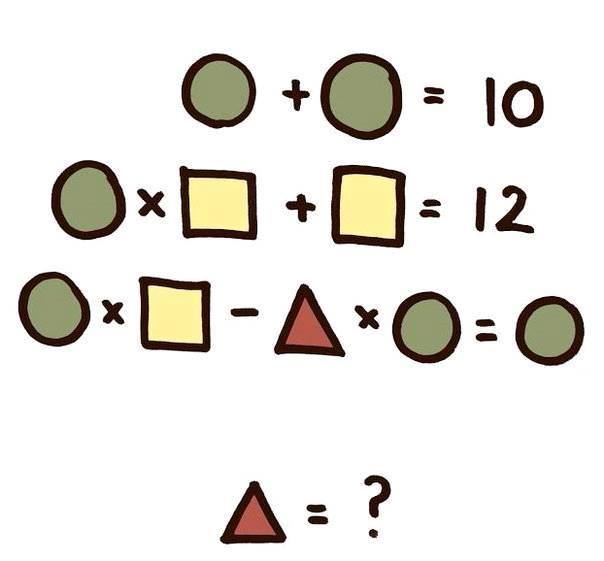
\includegraphics[scale=0.3]{basics/equation.jpg}
\caption{System of equations}
\end{figure}

It's that easy to solve it in Z3:

\begin{lstlisting}
#!/usr/bin/python
from z3 import *

circle, square, triangle = Ints('circle square triangle')
s = Solver()
s.add(circle+circle==10)
s.add(circle*square+square==12)
s.add(circle*square-triangle*circle==circle)
print s.check()
print s.model()
\end{lstlisting}

\begin{lstlisting}
sat
[triangle = 1, square = 2, circle = 5]
\end{lstlisting}

\subsection{Why variables are declared using declare-fun?}

They mean this is nullary function, only returning a constant, nothing else.

\subsection{Connection between \ac{SAT} and \ac{SMT} solvers}

\ac{SMT}-solvers are frontends to \ac{SAT} solvers, i.e.,
they translate inputted SMT expressions into \ac{CNF} and feed SAT-solver with it.
Translation process is sometimes called ``bit blasting''.
Some \ac{SMT}-solvers uses external SAT-solver: STP uses MiniSAT or CryptoMiniSAT as backend.
Some other \ac{SMT}-solvers (like Z3) has their own SAT solver.

\iffalse
\subsection{Theories}

...

QF\_S -- strings. You may need this to simulate strings to catch bugs like SQL injection.
\url{http://cvc4.cs.stanford.edu/wiki/Strings}.
\fi

% subsubsections:
\subsection{List of SMT-solvers}

\begin{itemize}

\item Yices\footnote{\url{http://yices.csl.sri.com/}}, created by Bruno Dutertre et al.

\item Z3\footnote{\url{https://github.com/Z3Prover/z3}},
developed by Leonardo de Moura, Nikolaj Bjorner, Christoph M. Wintersteiger, Lev Nachmanson.

Many examples here uses Python 2.x API for Z3 (AKA Z3Py).
Installation instructions (Ubuntu):

\begin{lstlisting}
sudo apt-get install python3-pip
sudo pip3 install z3-solver
\end{lstlisting}

Or compile the latest on Ubuntu:

\begin{lstlisting}
git clone https://github.com/Z3Prover/z3.git
cd z3
git tag
git checkout z3-4.8.4	# or another version
python scripts/mk_make.py --python
cd build
make
sudo make install
\end{lstlisting}

(Unofficial) bindings:
Haskell\footnote{\url{http://hackage.haskell.org/package/z3}},
Racket\footnote{\url{https://github.com/philnguyen/z3-rkt}},
Ruby\footnote{\url{https://github.com/prove-rs/z3.rs}}.

\item STP\footnote{\url{https://github.com/stp/stp}}, used in KLEE.

\item CVC3/CVC4\footnote{\url{http://cvc4.stanford.edu/}}.

\item Boolector\footnote{\url{http://fmv.jku.at/boolector/}}, developed by Aina Niemetz, Mathias Preiner and Armin Biere.
Known to be fastest bitvector solver.

\item Alt-Ergo\footnote{\url{https://alt-ergo.ocamlpro.com/}}, used in Frama-C.

\item MathSAT\footnote{\url{http://mathsat.fbk.eu/}}. Developed by Alberto Griggio, Alessandro Cimatti and Roberto Sebastiani.

\item veriT\footnote{\url{http://www.verit-solver.org/}}.
Developed by David Déharbe, Pascal Fontaine, Haniel Barbosa.
Lacks bitvectors.

\item toysolver\footnote{\url{https://github.com/msakai/toysolver}} by Masahiro Sakai, written in Haskell.

\item MK85\footnote{\url{https://github.com/DennisYurichev/MK85}}.
Created by Dennis Yurichev, as a toy bit-blaster, supports booleans and bitvectors.

\item dReal: ``An SMT Solver for Nonlinear Theories of the Reals''
\footnote{\url{http://dreal.cs.cmu.edu}, \url{https://github.com/dreal}}.

\end{itemize}

Something else:

\begin{itemize}

\item PySMT: unified Python interface to many SMT solvers: \url{https://pysmt.readthedocs.io/en/latest/}

\item JavaSMT -- Unified Java API for SMT solvers: \url{https://github.com/sosy-lab/java-smt}

\item jSMTLIB -- Another Java API for SMT solvers: \url{http://smtlib.github.io/jSMTLIB/}

\item SBV: SMT Based Verification in Haskell: \url{http://leventerkok.github.io/sbv/}

\end{itemize}


\subsection{Z3 specific}

The output is not guaranteed to be random.
You can randomize it by:

\begin{lstlisting}
import time

...

s=Solver()
set_param("smt.random_seed", int(time.time()))
\end{lstlisting}

Or conversely, you may want to reproduce its result each time the same:

\begin{lstlisting}
set_param("smt.random_seed", 1234)
\end{lstlisting}



\section{\ac{SAT}-solvers}

\renewcommand{\CURPATH}{basics/SAT}

SMT vs. SAT is like high level \ac{PL} vs. assembly language.
The latter can be much more efficient, but it's hard to program in it.

SAT is abbreviation of ``Boolean satisfiability problem''.
The problem is to find such a set of variables, which, if plugged into boolean expression, will result in ``true''.

\subsection{CNF form}

\ac{CNF}\footnote{\url{https://en.wikipedia.org/wiki/Conjunctive_normal_form}} is a \textit{normal form}.

% TODO recheck
% TODO write abt it!
%\textit{normal form} is somewhat similar to polynomials in algebra. 
%What is polynomial?
%It is a standard way to express unsystematic equations like $2x \cdot x$ as $3x$ polynomial, 
%and so you will be able to apply some operations to polynomials like summing, etc.

Any boolean expression can be converted to \textit{normal form} and \ac{CNF} is one of them.
The \ac{CNF} expression is a bunch of clauses (sub-expressions) constisting of terms (variables), ORs and NOTs, 
all of which are then glueled together with AND into a full expression.
There is a way to memorize it: \ac{CNF} is ``AND of ORs'' (or ``product of sums'') and \ac{DNF} is ``OR of ANDs'' (or ``sum of products'').

Example is: $(\neg A \vee B) \wedge (C \vee \neg D)$.

$\vee$ stands for OR (logical disjunction\footnote{\url{https://en.wikipedia.org/wiki/Logical_disjunction}}), 
``+'' sign is also sometimes used for OR.

$\wedge$ stands for AND (logical conjunction\footnote{\url{https://en.wikipedia.org/wiki/Logical_conjunction}}).
It is easy to memorize: $\wedge$ looks like ``A'' letter.
``$\cdot$'' is also sometimes used for AND.

$\neg$ is negation (NOT).

% TODO A/B is the first clause, C/D is second

\subsection{Example: 2-bit adder}
\label{adder}

\ac{SAT}-solver is merely a solver of huge boolean equations in CNF form.
It just gives the answer, if there is a set of input values which can satisfy CNF expression, and what input values must be.

Here is a 2-bit adder for example:

\begin{figure}[ht!]
\centering
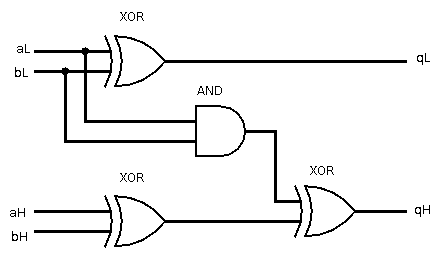
\includegraphics[scale=0.75]{\CURPATH/adder_logisim.png}
\caption{2-bit adder circuit}
\end{figure}

The adder in its simplest form: it has no carry-in and carry-out, and it has 3 XOR gates and one AND gate.
Let's try to figure out, which sets of input values will force adder to set both two output bits?
By doing quick memory calculation, we can see that there are 4 ways to do so: $0+3=3$, $1+2=3$, $2+1=3$, $3+0=3$.
Here is also truth table, with these rows highlighted:

\newcommand{\HLcell}{\cellcolor{blue!25}}

\begin{center}
\begin{doublespace}
\noindent\(\begin{array}{l|llllll}
  & \text{aH} & \text{aL} & \text{bH} & \text{bL} & \text{qH} & \text{qL} \\
\hline
 \text{3+3 = 6 $\equiv $ 2 (mod 4)} & 1 & 1 & 1 & 1 & 1 & 0 \\
 \text{3+2 = 5 $\equiv $ 1 (mod 4)} & 1 & 1 & 1 & 0 & 0 & 1 \\
 \text{3+1 = 4 $\equiv $ 0 (mod 4)} & 1 & 1 & 0 & 1 & 0 & 0 \\
 \text{\HLcell{}3+0 = 3 $\equiv $ 3 (mod 4)} & \HLcell{}1 & \HLcell{}1 & \HLcell{}0 & \HLcell{}0 & \HLcell{}1 & \HLcell{}1 \\
 \text{2+3 = 5 $\equiv $ 1 (mod 4)} & 1 & 0 & 1 & 1 & 0 & 1 \\
 \text{2+2 = 4 $\equiv $ 0 (mod 4)} & 1 & 0 & 1 & 0 & 0 & 0 \\
 \text{\HLcell{}2+1 = 3 $\equiv $ 3 (mod 4)} & \HLcell{}1 & \HLcell{}0 & \HLcell{}0 & \HLcell{}1 & \HLcell{}1 & \HLcell{}1 \\
 \text{2+0 = 2 $\equiv $ 2 (mod 4)} & 1 & 0 & 0 & 0 & 1 & 0 \\
 \text{1+3 = 4 $\equiv $ 0 (mod 4)} & 0 & 1 & 1 & 1 & 0 & 0 \\
 \text{\HLcell{}1+2 = 3 $\equiv $ 3 (mod 4)} & \HLcell{}0 & \HLcell{}1 & \HLcell{}1 & \HLcell{}0 & \HLcell{}1 & \HLcell{}1 \\
 \text{1+1 = 2 $\equiv $ 2 (mod 4)} & 0 & 1 & 0 & 1 & 1 & 0 \\
 \text{1+0 = 1 $\equiv $ 1 (mod 4)} & 0 & 1 & 0 & 0 & 0 & 1 \\
 \text{\HLcell{}0+3 = 3 $\equiv $ 3 (mod 4)} & \HLcell{}0 & \HLcell{}0 & \HLcell{}1 & \HLcell{}1 & \HLcell{}1 & \HLcell{}1 \\
 \text{0+2 = 2 $\equiv $ 2 (mod 4)} & 0 & 0 & 1 & 0 & 1 & 0 \\
 \text{0+1 = 1 $\equiv $ 1 (mod 4)} & 0 & 0 & 0 & 1 & 0 & 1 \\
 \text{0+0 = 0 $\equiv $ 0 (mod 4)} & 0 & 0 & 0 & 0 & 0 & 0 \\
\end{array}\)
\end{doublespace}
\end{center}


Let's find, what \ac{SAT}-solver can say about it?

First, we should represent our 2-bit adder as \ac{CNF} expression.

Using Wolfram Mathematica, we can express 1-bit expression for both adder outputs:\\
\\
\textbf{\texttt{In[]:=AdderQ0[aL$\_$,bL$\_$]=Xor[aL,bL]}} \\
\textbf{\texttt{Out[]:=aL $\veebar$ bL}} \\
\\
\textbf{\texttt{In[]:=AdderQ1[aL$\_$,aH$\_$,bL$\_$,bH$\_$]=Xor[And[aL,bL],Xor[aH,bH]]}} \\
\textbf{\texttt{Out[]:=aH $\veebar$ bH $\veebar$ (aL \&\& bL)}} \\
\\
We need such expression, where both parts will generate 1's.
Let's use Wolfram Mathematica find all instances of such expression (I glueled both parts with And): \\
\\
\textbf{\texttt{In[]:=Boole[SatisfiabilityInstances[And[AdderQ0[aL,bL],AdderQ1[aL,aH,bL,bH]],\{aL,aH,bL,bH\},4]]}} \\
\textbf{\texttt{Out[]:=\{1,1,0,0\},\{1,0,0,1\},\{0,1,1,0\},\{0,0,1,1\}}} \\
\\
Yes, indeed, Mathematica says, there are 4 inputs which will lead to the result we need.
So, Mathematica can also be used as \ac{SAT} solver.

Nevertheless, let's proceed to \ac{CNF} form. Using Mathematica again, let's convert our expression to \ac{CNF} form:\\
\\
\textbf{\texttt{In[]:=cnf=BooleanConvert[And[AdderQ0[aL,bL],AdderQ1[aL,aH,bL,bH]],``CNF'']}} \\
\textbf{\texttt{Out[]:=(!aH $\|$ !bH) \&\& (aH $\|$ bH) \&\& (!aL $\|$ !bL) \&\& (aL $\|$ bL)}} \\
\\
Looks more complex. The reason of such verbosity is that \ac{CNF} form doesn't allow XOR operations.
% FIXME: TeX form of the expression!

\subsubsection{MiniSat}

For starters, we can try MiniSat\footnote{\url{http://minisat.se/MiniSat.html}}.
The standard way to encode \ac{CNF} expression for MiniSat is to enumerate all OR parts at each line.
Also, MiniSat doesn't support variable names, just numbers.
Let's enumerate our variables: 1 will be aH, 2 -- aL, 3 -- bH, 4 -- bL.

Here is what I've got when I converted Mathematica expression to the MiniSat input file:

\lstinputlisting{\CURPATH/adder.cnf}

Two 4's at the first lines are number of variables and number of clauses respectively.
There are 4 lines then, each for each OR clause.
Minus before variable number meaning that the variable is negated.
Absence of minus -- not negated.
Zero at the end is just terminating zero, meaning end of the clause.

In other words, each line is OR-clause with optional negations,
and the task of MiniSat is to find such set of input, which can satisfy all lines in the input file.

That file I named as \textit{adder.cnf} and now let's try MiniSat:

\begin{lstlisting}
% minisat -verb=0 adder.cnf results.txt
SATISFIABLE
\end{lstlisting}

The results are in \textit{results.txt} file:

\begin{lstlisting}
SAT
-1 -2 3 4 0
\end{lstlisting}

This means, if the first two variables (aH and aL) will be \textit{false}, and the last two variables (bH and bL) will be set to \textit{true},
the whole \ac{CNF} expression is satisfiable.
Seems to be true: if bH and bL are the only inputs set to \textit{true}, both resulting bits are also has \textit{true} states.

Now how to get other instances? \ac{SAT}-solvers, like \ac{SMT} solvers, produce only one solution (or \textit{instance}).

MiniSat uses \ac{PRNG} and its initial seed can be set explicitely. I tried different values, but result is still the same.
Nevertheless, CryptoMiniSat in this case was able to show all possible 4 instances, in chaotic order, though.
So this is not very robust way.

Perhaps, the only known way is to negate solution clause and add it to the input expression.
We've got \TT{-1 -2 3 4}, 
now we can negate all values in it (just toggle minuses: \TT{1 2 -3 -4}) and add it to the end of the input file:

\begin{lstlisting}
p cnf 4 5
-1 -3 0
1 3 0
-2 -4 0
2 4 0
1 2 -3 -4
\end{lstlisting}

Now we've got another result:

\begin{lstlisting}
SAT
1 2 -3 -4 0
\end{lstlisting}

This means, aH and aL must be both \textit{true} and bH and bL must be \textit{false}, to satisfy the input expression.
Let's negate this clause and add it again:

\begin{lstlisting}
p cnf 4 6
-1 -3 0
1 3 0
-2 -4 0
2 4 0
1 2 -3 -4
-1 -2 3 4 0
\end{lstlisting}

The result is:

\begin{lstlisting}
SAT
-1 2 3 -4 0
\end{lstlisting}

aH=false, aL=true, bH=true, bL=false. This is also correct, according to our truth table.

Let's add it again:

\begin{lstlisting}
p cnf 4 7
-1 -3 0
1 3 0
-2 -4 0
2 4 0
1 2 -3 -4
-1 -2 3 4 0
1 -2 -3 4 0
\end{lstlisting}

\begin{lstlisting}
SAT
1 -2 -3 4 0
\end{lstlisting}

\textit{aH=true, aL=false, bH=false, bL=true.} This is also correct.

This is fourth result. There are shouldn't be more. What if to add it?

\begin{lstlisting}
p cnf 4 8
-1 -3 0
1 3 0
-2 -4 0
2 4 0
1 2 -3 -4
-1 -2 3 4 0
1 -2 -3 4 0
-1 2 3 -4 0
\end{lstlisting}

Now MiniSat just says ``UNSATISFIABLE'' without any additional information in the resulting file.

Our example is tiny, but MiniSat can work with huge \ac{CNF} expressions.

\subsubsection{CryptoMiniSat}

XOR operation is absent in \ac{CNF} form, but crucial in cryptographical algorithms.
Simplest possible way to represent single XOR operation in \ac{CNF} form is:
$(\neg x \vee \neg y) \wedge (x \vee y)$ -- not that small expression, 
though, many XOR operations in single expression can be optimized better.

One significant difference between MiniSat and CryptoMiniSat is that
the latter supports clauses with XOR operations instead of ORs,
because CryptoMiniSat has aim to analyze crypto algorithms\footnote{\url{http://www.msoos.org/xor-clauses/}}.
XOR clauses are handled by CryptoMiniSat in a special way without translating to OR clauses.

You need just to prepend a clause with ``x'' in \ac{CNF} file and OR clause is then treated as XOR clause by CryptoMiniSat.
As of 2-bit adder, this smallest possible XOR-CNF expression can be used to find all inputs where both output adder bits are set:

$(aH \oplus bH) \wedge (aL \oplus bL)$

This is \TT{.cnf} file for CryptoMiniSat:

\begin{lstlisting}
p cnf 4 2
x1 3 0
x2 4 0
\end{lstlisting}

Now I run CryptoMiniSat with various random values to initialize its \ac{PRNG} \dots

\begin{lstlisting}
% cryptominisat4 --verb 0 --random 0 XOR_adder.cnf
s SATISFIABLE
v 1 2 -3 -4 0
% cryptominisat4 --verb 0 --random 1 XOR_adder.cnf
s SATISFIABLE
v -1 -2 3 4 0
% cryptominisat4 --verb 0 --random 2 XOR_adder.cnf
s SATISFIABLE
v 1 -2 -3 4 0
% cryptominisat4 --verb 0 --random 3 XOR_adder.cnf
s SATISFIABLE
v 1 2 -3 -4 0
% cryptominisat4 --verb 0 --random 4 XOR_adder.cnf
s SATISFIABLE
v -1 2 3 -4 0
% cryptominisat4 --verb 0 --random 5 XOR_adder.cnf
s SATISFIABLE
v -1 2 3 -4 0
% cryptominisat4 --verb 0 --random 6 XOR_adder.cnf
s SATISFIABLE
v -1 -2 3 4 0
% cryptominisat4 --verb 0 --random 7 XOR_adder.cnf
s SATISFIABLE
v 1 -2 -3 4 0
% cryptominisat4 --verb 0 --random 8 XOR_adder.cnf
s SATISFIABLE
v 1 2 -3 -4 0
% cryptominisat4 --verb 0 --random 9 XOR_adder.cnf
s SATISFIABLE
v 1 2 -3 -4 0
\end{lstlisting}

Nevertheless, all 4 possible solutions are:

\begin{lstlisting}
v -1 -2 3 4 0
v -1 2 3 -4 0
v 1 -2 -3 4 0
v 1 2 -3 -4 0
\end{lstlisting}

\dots the same as reported by MiniSat.

\subsection{Picosat}

At least Picosat can enumerate all possible solutions without crutches I just shown:

\begin{lstlisting}
% picosat --all adder.cnf
s SATISFIABLE
v -1 -2 3 4 0
s SATISFIABLE
v -1 2 3 -4 0
s SATISFIABLE
v 1 2 -3 -4 0
s SATISFIABLE
v 1 -2 -3 4 0
s SOLUTIONS 4
\end{lstlisting}

% subsubsections:
\subsubsection{MaxSAT}

MaxSAT problem is a problem where as many clauses should be satisfied, as possible, but maybe not all.

(Usual) clauses which \textit{must} be satisfied, called \textit{hard clauses}.
Clauses which \textit{should} be satisfied, called \textit{soft clauses}.

MaxSAT solver tries to satisfy all \textit{hard clauses} and as much \textit{soft clauses}, as possible.

*.wcnf files are used, the format is almost the same as in DIMACS files, like:

\begin{lstlisting}
p wcnf 207 796 208
208 1 0
208 2 0
208 3 0
208 4 0

...

1 -152 0
1 -153 0
1 -154 0
1 155 0
1 -156 0
1 -157 0
\end{lstlisting}

Each clause is written as in DIMACS file, but the first number if weight.
MaxSAT solver tries to maximize clauses with bigger weights first.

If the weight has \textit{top weight}, the clause is \textit{hard clause} and must always be satisfied.
\textit{Top weight} is set in header.
In our case, it's 208.

Some well-known MaxSAT solvers are Open-WBO\footnote{\url{http://sat.inesc-id.pt/open-wbo}}, etc.


\subsection{List of SAT-solvers}

% TODO authors, URLs

\begin{itemize}

\item MiniSat\footnote{http://minisat.se/}, serving as a base for others

\item PicoSat, PrecoSat, Lingeling. Created by Armin Biere. Plingeling supports multithreading.

\item CryptoMiniSat. Created by Mate Soos for cryptographical problems exploration.
Supports XOR clauses, multithreading.
Has Python API.

\end{itemize}






\EN{\chapter{Equations}

% subsections:
\section{Solving XKCD 287}
\label{XkcdILP}

\begin{figure}[H]
\centering
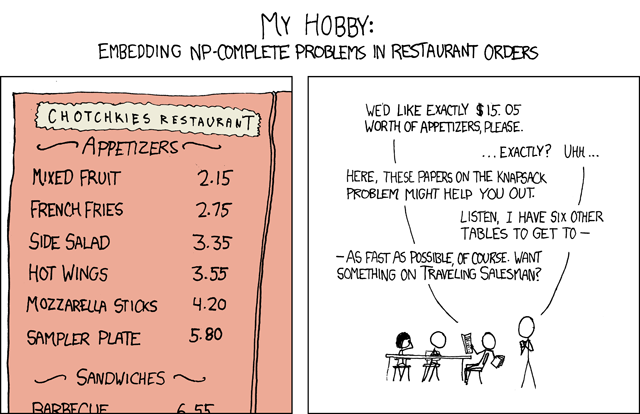
\includegraphics[scale=7]{equations/xkcd287/np_complete.png}
\caption{xkcd \#287}
\end{figure}

( \url{https://www.xkcd.com/287/} )

The problem is to solve the following equation:
$2.15a + 2.75b + 3.35c + 3.55d + 4.20e + 5.80f == 15.05$,
where a..f are integers.
So this is a linear diophantine equation.

\lstinputlisting[style=custompy]{equations/xkcd287/xkcd287_MK85.py}

( The source code: \url{https://github.com/DennisYurichev/SAT_SMT_by_example/blob/master/equations/xkcd287/xkcd287_MK85.py} )

There are just 2 solutions:

\begin{lstlisting}
{'a': 7, 'c': 0, 'b': 0, 'e': 0, 'd': 0, 'f': 0}
{'a': 1, 'c': 0, 'b': 0, 'e': 0, 'd': 2, 'f': 1}
\end{lstlisting}

Wolfram Mathematica can solve the equation as well:

\begin{lstlisting}
In[]:= FindInstance[2.15 a + 2.75 b + 3.35 c + 3.55 d + 4.20 e + 5.80 f == 15.05 && 
	a >= 0 && b >= 0 && c >= 0 && d >= 0  && e >= 0 && f >= 0, 
	{a, b, c, d, e, f}, Integers, 1000]

Out[]= {{a -> 1, b -> 0, c -> 0, d -> 2, e -> 0, f -> 1},
	{a -> 7, b -> 0, c -> 0, d -> 0, e -> 0, f -> 0}}
\end{lstlisting}

1000 means ``find at most 1000 solutions'', but only 2 are found.
See also: \url{http://reference.wolfram.com/language/ref/FindInstance.html}.\\
\\
Other ways to solve it:
\url{https://stackoverflow.com/questions/141779/solving-the-np-complete-problem-in-xkcd},
\url{http://www.explainxkcd.com/wiki/index.php/287:_NP-Complete}.

The solution using Z3: \url{https://github.com/DennisYurichev/SAT_SMT_by_example/blob/master/equations/xkcd287/xkcd287_Z3.py} )

\section{XKCD 287 in SMT-LIB 2.x format}

\lstinputlisting[style=customsmt]{equations/xkcd287/xkcd287.smt}

\section{Other solutions}

Some other solutions, including the one using Prolog:
\url{https://stackoverflow.com/q/141779}.


\section{Art of problem solving}

\url{http://artofproblemsolving.com/wiki/index.php?title=2017_AMC_12A_Problems/Problem_2}:

\begin{lstlisting}
The sum of two nonzero real numbers is 4 times their product.
What is the sum of the reciprocals of the two numbers? 
\end{lstlisting}

We're going to solve this over real numbers:

\begin{lstlisting}[style=custompy]
from z3 import *

x, y = Reals('x y')

s=Solver()

s.add(x>0)
s.add(y>0)

s.add(x+y == 4*x*y)

print s.check()
m=s.model()
print "the model:"
print m
print "the answer:", m.evaluate (1/x + 1/y)
\end{lstlisting}

Instead of pulling values from the model and then compute the final result on Python's side, we can evaluate
an expression ($\frac{1}{x} + \frac{1}{y}$) \emph{inside} the model we've got:

\begin{lstlisting}
sat
the model:
[x = 1, y = 1/3]
the answer: 4
\end{lstlisting}


\section{Yet another explanation of modulo inverse using SMT-solvers}

\MathForProg has a part about modulo arithmetics and modulo inverse.

By which constant we must multiply a random number, so that the result would be as if we divided them by 3?

\begin{lstlisting}
from z3 import *

m=BitVec('m', 32)

s=Solver()

# wouldn't work for 10, etc
divisor=3

# random constant, must be divisible by divisor:
const=(0x1234567*divisor)

s.add(const*m == const/divisor)

print s.check()
print "%x" % s.model()[m].as_long()
\end{lstlisting}

The magic number is:

\begin{lstlisting}
sat
aaaaaaab
\end{lstlisting}

Indeed, this is modulo inverse of 3 modulo $2^{32}$: \url{https://www.wolframalpha.com/input/?i=PowerMod%5B3,-1,2%5E32%5D}.

Let's check using \href{https://github.com/DennisYurichev/progcalc}{my calculator}:

\begin{lstlisting}
[3] 123456*0xaaaaaaab
[3] (unsigned) 353492988371136 0x141800000a0c0 0b1010000011000000000000000000000001010000011000000
[4] 123456/3
[4] (unsigned) 41152 0xa0c0 0b1010000011000000
\end{lstlisting}

The problem is simple enough to be solved using MK85:

\lstinputlisting[style=customsmt]{equations/modinv/modinv.smt}

\lstinputlisting{equations/modinv/modinv.correct}

However, it wouldn't work for 10, because there are no modulo inverse of 10 modulo $2^{32}$, SMT solver would give "unsat".


\subsection{School-level equation}

Let's revisit school-level system of equations from (\ref{eq2_SMT}).

We will force KLEE to find a path, where all the constraints are satisfied:

\lstinputlisting[style=customc]{equations/KLEE_eq/klee_eq1.c}

% FIXME:
\begin{lstlisting}
% clang -emit-llvm -c -g klee_eq.c
...

% klee klee_eq.bc
KLEE: output directory is "/home/klee/klee-out-93"
KLEE: WARNING: undefined reference to function: klee_assert
KLEE: WARNING ONCE: calling external: klee_assert(0)
KLEE: ERROR: /home/klee/klee_eq.c:18: failed external call: klee_assert
KLEE: NOTE: now ignoring this error at this location

KLEE: done: total instructions = 32
KLEE: done: completed paths = 1
KLEE: done: generated tests = 1
\end{lstlisting}

Let's find out, where \TT{klee\_assert()} has been triggered:

% FIXME:
\begin{lstlisting}
% ls klee-last | grep err
test000001.external.err

% ktest-tool --write-ints klee-last/test000001.ktest
ktest file : 'klee-last/test000001.ktest'
args       : ['klee_eq.bc']
num objects: 3
object    0: name: b'circle'
object    0: size: 4
object    0: data: 5
object    1: name: b'square'
object    1: size: 4
object    1: data: 2
object    2: name: b'triangle'
object    2: size: 4
object    2: data: 1
\end{lstlisting}

This is indeed correct solution to the system of equations.

KLEE has \textit{intrinsic} \TT{klee\_assume()} which tells KLEE to cut path if some constraint is not satisfied.
So we can rewrite our example in such cleaner way:

\lstinputlisting[style=customc]{equations/KLEE_eq/klee_eq2.c}



\section{Minesweeper}

% subsections:
\input{equations/minesweeper/1_SMT/main_EN.tex}
\input{equations/minesweeper/2_SAT/main_EN.tex}
\input{equations/minesweeper/3_SMT_opt/main_EN.tex}
\input{equations/minesweeper/4_Knuth/main_EN.tex}


\subsection{Cracking \ac{LCG} with Z3}

There are well-known weaknesses of \ac{LCG}
\footnote{\url{http://en.wikipedia.org/wiki/Linear_congruential_generator\#Advantages_and_disadvantages_of_LCGs},
\url{http://www.reteam.org/papers/e59.pdf},
\url{http://stackoverflow.com/questions/8569113/why-1103515245-is-used-in-rand/8574774\#8574774}},
but let's see, if it would be possible to crack it straightforwardly, without any special knowledge.
We will define all relations between LCG states in terms of Z3.
Here is a test progam:

\begin{lstlisting}
#include <stdlib.h>
#include <stdio.h>
#include <time.h>

int main()
{
	int i;

	srand(time(NULL));

	for (i=0; i<10; i++)
		printf ("%d\n", rand()%100);
};
\end{lstlisting}

It is printing 10 pseudorandom numbers in 0..99 range:

\begin{lstlisting}
37
29
74
95
98
40
23
58
61
17
\end{lstlisting}

Let's say we are observing only 8 of these numbers (from 29 to 61) and we need to predict next one (17) and/or previous one (37).

The program is compiled using MSVC 2013 (I choose it because its LCG is simpler than that in Glib):

\begin{lstlisting}
.text:0040112E rand            proc near
.text:0040112E                 call    __getptd
.text:00401133                 imul    ecx, [eax+0x14], 214013
.text:0040113A                 add     ecx, 2531011
.text:00401140                 mov     [eax+14h], ecx
.text:00401143                 shr     ecx, 16
.text:00401146                 and     ecx, 7FFFh
.text:0040114C                 mov     eax, ecx
.text:0040114E                 retn
.text:0040114E rand            endp
\end{lstlisting}

Let's define \ac{LCG} in Z3Py:

\begin{lstlisting}
#!/usr/bin/python
from z3 import *

output_prev = BitVec('output_prev', 32)
state1 = BitVec('state1', 32)
state2 = BitVec('state2', 32)
state3 = BitVec('state3', 32)
state4 = BitVec('state4', 32)
state5 = BitVec('state5', 32)
state6 = BitVec('state6', 32)
state7 = BitVec('state7', 32)
state8 = BitVec('state8', 32)
state9 = BitVec('state9', 32)
state10 = BitVec('state10', 32)
output_next = BitVec('output_next', 32)

s = Solver()

s.add(state2 == state1*214013+2531011)
s.add(state3 == state2*214013+2531011)
s.add(state4 == state3*214013+2531011)
s.add(state5 == state4*214013+2531011)
s.add(state6 == state5*214013+2531011)
s.add(state7 == state6*214013+2531011)
s.add(state8 == state7*214013+2531011)
s.add(state9 == state8*214013+2531011)
s.add(state10 == state9*214013+2531011)

s.add(output_prev==URem((state1>>16)&0x7FFF,100))
s.add(URem((state2>>16)&0x7FFF,100)==29)
s.add(URem((state3>>16)&0x7FFF,100)==74)
s.add(URem((state4>>16)&0x7FFF,100)==95)
s.add(URem((state5>>16)&0x7FFF,100)==98)
s.add(URem((state6>>16)&0x7FFF,100)==40)
s.add(URem((state7>>16)&0x7FFF,100)==23)
s.add(URem((state8>>16)&0x7FFF,100)==58)
s.add(URem((state9>>16)&0x7FFF,100)==61)
s.add(output_next==URem((state10>>16)&0x7FFF,100))

print(s.check())
print(s.model())
\end{lstlisting}

\textit{URem} states for \textit{unsigned remainder}.
It works for some time and gave us correct result!

\begin{lstlisting}
sat
[state3 = 2276903645,
 state4 = 1467740716,
 state5 = 3163191359,
 state7 = 4108542129,
 state8 = 2839445680,
 state2 = 998088354,
 state6 = 4214551046,
 state1 = 1791599627,
 state9 = 548002995,
 output_next = 17,
 output_prev = 37,
 state10 = 1390515370]
\end{lstlisting}

I added $\approx 10$ states to be sure result will be correct.
It may be not in case of smaller set of information.

That is the reason why \ac{LCG} is not suitable for any security-related task.
This is why cryptographically secure pseudorandom number generators exist:
they are designed to be protected against such simple attack.
Well, at least if \ac{NSA} don't get involved
\footnote{\url{https://en.wikipedia.org/wiki/Dual_EC_DRBG}}.

Security tokens like ``RSA SecurID'' can be viewed just as \ac{CPRNG} with a secret seed.
It shows new pseudorandom number each minute, and the server can predict it, because it knows the seed.
Imagine if such token would implement \ac{LCG}---it would be much easier to break!


\section{Can rand() generate 10 consecutive zeroes?}

\renewcommand{\CURPATH}{equations/LCG}

I've always been wondering, if it's possible or not.
As of simplest linear congruential generator from MSVC's rand(), I could get a state at which rand() will output 8 zeroes modulo 10:

\lstinputlisting[style=custompy]{\CURPATH/LCG10.py}

\begin{lstlisting}
sat
[state3 = 1181667981,
 state4 = 342792988,
 state5 = 4116856175,
 state7 = 1741999969,
 state8 = 3185636512,
 state2 = 1478548498,
 state6 = 4036911734,
 state1 = 286227003,
 state9 = 1700675811]
\end{lstlisting}

This is a case if, in some video game, you'll find a code:

\begin{lstlisting}
for (int i=0; i<8; i++)
    printf ("%d\n", rand() % 10);
\end{lstlisting}

... and at some point, this piece of code can generate 8 zeroes in row, if the state will be 286227003 (decimal).

Just checked this piece of code in MSVC 2015:

\begin{lstlisting}
// MSVC 2015 x86

#include <stdio.h>

int main()
{
	srand(286227003);

	for (int i=0; i<8; i++)
		printf ("%d\n", rand() % 10);
};
\end{lstlisting}

Yes, its output is 8 zeroes!

What about other modulos?

I can get 4 consecutive zeroes modulo 100:

\lstinputlisting[style=custompy]{\CURPATH/LCG100.py}

\begin{lstlisting}
sat
[state3 = 635704497,
 state4 = 1644979376,
 state2 = 1055176198,
 state1 = 3865742399,
 state5 = 1389375667]
\end{lstlisting}

However, 4 consecutive zeroes modulo 100 is impossible (given these constants at least), this gives ``unsat'':
\url{https://github.com/DennisYurichev/SAT_SMT_by_example/blob/master/equations/LCG/LCG100_v1.py}.

... and 3 consecutive zeroes modulo 1000:

\lstinputlisting[style=custompy]{\CURPATH/LCG1000.py}

\begin{lstlisting}
sat
[state3 = 1179663182,
 state2 = 720934183,
 state1 = 4090229556,
 state4 = 786474201]
\end{lstlisting}

What if we could use rand()'s output without division? Which is in 0..0x7fff range (i.e., 15 bits)?
As it can be checked quickly, 2 zeroes at output is possible:

\lstinputlisting[style=custompy]{\CURPATH/LCG.py}

\begin{lstlisting}
sat
[state2 = 20057, state1 = 3385131726, state3 = 22456]
\end{lstlisting}

\subsection{UNIX time and srand(time(NULL))}

Given the fact that it's highly popular to initialize LCG PRNG with UNIX time (i.e., \TT{srand(time(NULL))}), you can probably calculate a moment in time so that LCG PRNG will be initialized as you want to.

For example, can we get a moment in time from now (5-Dec-2017) till 12-Dec-2017 (that is one week from now), when, if initialized by UNIX time, rand() will output as many similar numbers (modulo 10), as possible?

\lstinputlisting[style=custompy]{\CURPATH/LCG10_time.py}

Yes:

\begin{lstlisting}
sat
[state3 = 2234253076,
 state4 = 497021319,
 state5 = 4160988718,
 c = 3,
 state2 = 333151205,
 state6 = 46785593,
 state1 = 1512500810,
 state7 = 1158878744]
\end{lstlisting}

If \TT{srand(time(NULL))} will be executed at \TT{Tue Dec  5 21:06:50 EET 2017} (this precise second, UNIX time=1512500810),
a next 6 \TT{rand() \% 10} lines will output six numbers of 3 in a row.
Don't know if it useful or not, but you've got the idea.

\subsection{etc:}

The files: \url{https://github.com/DennisYurichev/SAT_SMT_by_example/tree/master/equations/LCG}.

Further work: check glibc's \TT{rand()}, Mersenne Twister, etc. Simple 32-bit LCG as described can be checked using simple brute-force, I think.

\subsection{Fun story}

The software checked protection key (dongle) randomly, from time to time.
This code snippet is from a real one:

\begin{lstlisting}[style=customc]
void init_all()
{
	...

	srand(time(NULL));

	...
};

...

void check_protection_thread()
{
	// get in 0..9 range
	int t=(int)((double)rand()/3276);
	if (t== 5)
	{
		check protection
	}
};
\end{lstlisting}

Perhaps, we can find the most optimal UNIX time to start the software, so the protection will not be checked as long as possible...

\subsection{Further reading}

Breaking JavaScript's \ac{PRNG} (XorShift128+):
\url{https://blog.securityevaluators.com/hacking-the-javascript-lottery-80cc437e3b7f}.


\subsection{Integer factorization using Z3 SMT solver}
\label{factor_Z3}

Integer factorization is method of breaking a composite (non-prime number) into prime factors.
Like 12345 = 3*4*823.

Though for small numbers, this task can be accomplished by Z3:

\lstinputlisting[style=custompy]{equations/factor_SMT/factor_z3.py}

( The source code: \url{https://github.com/DennisYurichev/SAT_SMT_by_example/blob/master/equations/factor_SMT/factor_z3.py} )

When factoring 1234567890 recursively:

\begin{lstlisting}
% time python z.py
factoring 1234567890
factors of 1234567890 are 342270 and 3607
factoring 342270
factors of 342270 are 2 and 171135
factoring 2
2 is prime (unsat)
factoring 171135
factors of 171135 are 3803 and 45
factoring 3803
3803 is prime (unsat)
factoring 45
factors of 45 are 3 and 15
factoring 3
3 is prime (unsat)
factoring 15
factors of 15 are 5 and 3
factoring 5
5 is prime (unsat)
factoring 3
3 is prime (unsat)
factoring 3607
3607 is prime (unsat)
[2, 3, 3, 5, 3607, 3803]
python z.py  19.30s user 0.02s system 99% cpu 19.443 total
\end{lstlisting}

So, 1234567890 = 2*3*3*5*3607*3803.

One important note: there is no primality test, no lookup tables, etc.
Prime number is a number for which "x*y=prime" (where x>1 and y>1) diophantine equation (which allows only integers in solution) has no solutions.
It can be solved for real numbers, though.

Z3 is \href{https://github.com/Z3Prover/z3/issues/1264}{not yet good enough for non-linear integer arithmetic}
and sometimes returns "unknown" instead of "unsat", but,
as Leonardo de Moura (one of Z3's author) commented about this:

\begin{lstlisting}
...Z3 will solve the problem as a real problem. If no real solution is found, we know there is no integer solution.
If a solution is found, Z3 will check if the solution is really assigning integer values to integer variables.
If that is not the case, it will return unknown to indicate it failed to solve the problem.
\end{lstlisting}
( \url{https://stackoverflow.com/questions/13898175/how-does-z3-handle-non-linear-integer-arithmetic} )

Probably, this is the case: we getting "unknown" in the case when a number cannot be factored, i.e., it's prime.

It's also very slow. Wolfram Mathematica can factor number around $2^{80}$ in a matter of seconds.
Still, I've written this for demonstration.

The problem of breaking \ac{RSA} is a problem of factorization of very large numbers, up to $2^{4096}$.
It's currently not possible to do this in practice.


\subsection{Integer factorization using SAT solver}
\label{factor_SAT}

\renewcommand{\CURPATH}{equations/factor_SAT}

See also: integer factorization using Z3 SMT solver (\ref{factor_Z3}).

We are going to simulate electronic circuit of binary multiplier in SAT and then ask solver, what multiplier's inputs must be so the output will be a desired number?
If this situation is impossible, the desired number is prime.

First we should build multiplier out of adders.

\subsubsection{Binary adder in SAT}

Simple binary adder usually constists of full-adders and one half-adder.
These are basic elements of adders.

% FIXME: TikZ!
\begin{figure}[H]
\centering
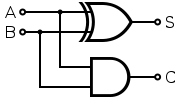
\includegraphics[scale=1]{\CURPATH/half_adder.png}
\caption{Half-adder}
\end{figure}

( The image has been taken from \href{https://en.wikipedia.org/wiki/Adder_(electronics)}{Wikipedia}. )

Full-adder:

% FIXME: TikZ!
\begin{figure}[H]
\centering
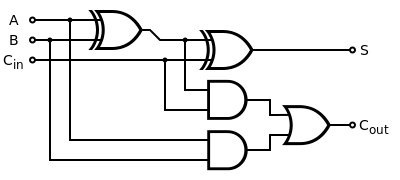
\includegraphics[scale=1]{\CURPATH/full_adder.png}
\caption{Full-adder}
\end{figure}

( The image has been taken from \href{https://en.wikipedia.org/wiki/Adder_(electronics)}{Wikipedia}. )

Here is a 4-bit ripple-carry adder:

% TikZ!
\begin{lstlisting}
         X3 Y3              X2 Y2              X1 Y1              X0 Y0
         |  |               |  |               |  |               |  |
         v  v               v  v               v  v               v  v
        +----+             +----+             +----+             +----+
Cout <- | FA | <- carry <- | FA | <- carry <- | FA | <- carry <- | HA |
        +----+             +----+             +----+             +----+
          ^                  ^                  ^                  ^
          |                  |                  |                  |
          S3                 S2                 S1                 S0
\end{lstlisting}

It can be used for most tasks.

Here is a 4-bit ripple-carry adder with carry-in:

\begin{lstlisting}
         X3 Y3              X2 Y2              X1 Y1              X0 Y0
         |  |               |  |               |  |               |  |
         v  v               v  v               v  v               v  v
        +----+             +----+             +----+             +----+
Cout <- | FA | <- carry <- | FA | <- carry <- | FA | <- carry <- | FA | <- Cin
        +----+             +----+             +----+             +----+
          ^                  ^                  ^                  ^
          |                  |                  |                  |
          S3                 S2                 S1                 S0
\end{lstlisting}

What carries are?
4-bit adder can sum up two numbers up to 0b1111 (15).
15+15=30 and this is 0b11110, i.e., 5 bits. Lowest 4 bits is a sum.
5th most significant bit is not a part of sum, but is a carry bit.

If you sum two numbers on x86 CPU, CF flag is a carry bit connected to \ac{ALU}.
It is set if a resulting sum is bigger than it can be fit into result.

Now you can also need carry-in.
Again, x86 CPU has ADC instruction, it takes CF flag state.
It can be said, CF flag is connected to adder's carry-in input.
Hence, combining two ADD and ADC instructions you can sum up 128 bits on 64-bit CPU.

By the way, this is a good explanation of "carry-ripple".
The very first full-adder's result is depending on the carry-out of the previous full-adder.
Hence, adders cannot work in parallel.
This is a problem of simplest possible adder, other adders can solve this.

To represent full-adders in CNF form, we can use Wolfram Mathematica.
I've taken truth table for full-adder from \href{https://en.wikipedia.org/wiki/Adder_(electronics)}{Wikipedia}:

% FIXME: table!
\begin{lstlisting}
Inputs 	|  Outputs
--------+----------
A B Cin |  Cout Sum
0 0 0   |  0    0
0 0 1   |  0    1
0 1 0   |  0    1
0 1 1   |  1    0
1 0 0   |  0    1
1 0 1   |  1    0
1 1 0   |  1    0
1 1 1   |  1    1
\end{lstlisting}

In Mathematica, I'm setting "->1" if row is correct and "->0" if not correct.

\begin{lstlisting}
In[59]:= FaTbl = {{0, 0, 0, 0, 0} -> 1, {0, 0, 0, 0, 1} -> 
   0, {0, 0, 0, 1, 0} -> 0, {0, 0, 0, 1, 1} -> 0, {0, 0, 1, 0, 0} -> 
   0, {0, 0, 1, 0, 1} -> 1, {0, 0, 1, 1, 0} -> 0, {0, 0, 1, 1, 1} -> 
   0, {0, 1, 0, 0, 0} -> 0, {0, 1, 0, 0, 1} -> 1, {0, 1, 0, 1, 0} -> 
   0, {0, 1, 0, 1, 1} -> 0, {0, 1, 1, 0, 0} -> 0, {0, 1, 1, 0, 1} -> 
   0, {0, 1, 1, 1, 0} -> 1, {0, 1, 1, 1, 1} -> 0, {1, 0, 0, 0, 0} -> 
   0, {1, 0, 0, 0, 1} -> 1, {1, 0, 0, 1, 0} -> 0, {1, 0, 0, 1, 1} -> 
   0, {1, 0, 1, 0, 0} -> 0, {1, 0, 1, 0, 1} -> 0, {1, 0, 1, 1, 0} -> 
   1, {1, 0, 1, 1, 1} -> 0, {1, 1, 0, 0, 0} -> 0, {1, 1, 0, 0, 1} -> 
   0, {1, 1, 0, 1, 0} -> 1, {1, 1, 0, 1, 1} -> 0, {1, 1, 1, 0, 0} -> 
   0, {1, 1, 1, 0, 1} -> 0, {1, 1, 1, 1, 0} -> 0, {1, 1, 1, 1, 1} -> 1}

...

In[60]:= BooleanConvert[
 BooleanFunction[FaTbl, {a, b, cin, cout, s}], "CNF"]

Out[60]= (! a || ! b || ! cin || s) && (! a || ! b || 
   cout) && (! a || ! cin || cout) && (! a || cout || s) && (a || b ||
    cin || ! s) && (a || b || ! cout) && (a || 
   cin || ! cout) && (a || ! cout || ! s) && (! b || ! cin || 
   cout) && (! b || cout || s) && (b || 
   cin || ! cout) && (b || ! cout || ! s) && (! cin || cout || 
   s) && (cin || ! cout || ! s)
\end{lstlisting}

These clauses can be used as full-adder.

Here is it:

\begin{lstlisting}
    # full-adder, as found by Mathematica using truth table:
    def FA (self, a,b,cin):
        s=self.create_var()
        cout=self.create_var()

        self.add_clause([self.neg(a), self.neg(b), self.neg(cin), s])
        self.add_clause([self.neg(a), self.neg(b), cout])
        self.add_clause([self.neg(a), self.neg(cin), cout])
        self.add_clause([self.neg(a), cout, s])
        self.add_clause([a, b, cin, self.neg(s)])
        self.add_clause([a, b, self.neg(cout)])
        self.add_clause([a, cin, self.neg(cout)])
        self.add_clause([a, self.neg(cout), self.neg(s)])
        self.add_clause([self.neg(b), self.neg(cin), cout])
        self.add_clause([self.neg(b), cout, s])
        self.add_clause([b, cin, self.neg(cout)])
        self.add_clause([b, self.neg(cout), self.neg(s)])
        self.add_clause([self.neg(cin), cout, s])
        self.add_clause([cin, self.neg(cout), self.neg(s)])

        return s, cout
\end{lstlisting}

And the adder:

\begin{lstlisting}
    # bit order: [MSB..LSB]
    # n-bit adder:
    def adder(self, X,Y):
        assert len(X)==len(Y)
        # first full-adder could be half-adder
        # start with lowest bits:
        inputs=my_utils.rvr(list(zip(X,Y)))
        carry=self.const_false
        sums=[]
        for pair in inputs:
            # "carry" variable is replaced at each iteration.
            # so it is used in the each FA() call from the previous FA() call.
            s, carry = self.FA(pair[0], pair[1], carry)
            sums.append(s)
        return my_utils.rvr(sums), carry
\end{lstlisting}

\subsubsection{Binary multiplier in SAT}

Remember school-level long division?
This multiplier works in a same way, but for binary digits.

Here is example of multiplying 0b1101 (X) by 0b0111 (Y):

% TikZ!
\begin{lstlisting}
         LSB
          |
          v
       1101 <- X
       -------
LSB 0|    0000
    1|   1101
    1|  1101
    1| 1101
    ^
    |
    Y
\end{lstlisting}

If bit from Y is zero, a row is zero.
If bit from Y is non-zero, a row is equal to X, but shifted each time.
Then you just sum up all rows (which are called "partial products".)

This is 4-bit binary multiplier. It takes 4-bit inputs and produces 8-bit output:

% FIXME: TikZ!
\begin{figure}[H]
\centering
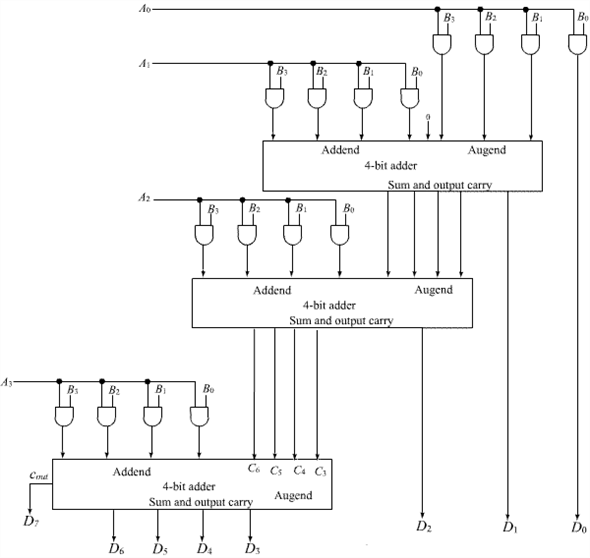
\includegraphics[scale=1]{\CURPATH/bin_mult.png}
\caption{4-bit binary multiplier}
\end{figure}

( The image has been taken from \url{http://www.chegg.com/homework-help/binary-multiplier-multiplies-two-unsigned-four-bit-numbers-u-chapter-4-problem-20p-solution-9780132774208-exc}. )

I would build separate block, "multiply by one bit" as a latch for each partial product:

\begin{lstlisting}
    def AND_Tseitin(self, v1, v2, out):
        self.add_clause([self.neg(v1), self.neg(v2), out])
        self.add_clause([v1, self.neg(out)])
        self.add_clause([v2, self.neg(out)])
    
    def AND(self,v1, v2):
        out=self.create_var()
        self.AND_Tseitin(v1, v2, out)
        return out

...

    # bit is 0 or 1.
    # i.e., if it's 0, output is 0 (all bits)
    # if it's 1, output=input
    def mult_by_bit(self, X, bit):
        return [self.AND(i, bit) for i in X]

    # bit order: [MSB..LSB]
    # build multiplier using adders and mult_by_bit blocks:
    def multiplier(self, X, Y):
        assert len(X)==len(Y)
        out=[]
        #initial:
        prev=[self.const_false]*len(X)
        # first adder can be skipped, but I left thing "as is" to make it simpler
        for Y_bit in my_utils.rvr(Y):
            s, carry = self.adder(self.mult_by_bit(X, Y_bit), prev)
            out.append(s[-1])
            prev=[carry] + s[:-1]
    
        return prev + my_utils.rvr(out)
\end{lstlisting}

AND gate is constructed here using Tseitin transformations.
This is quite popular way of encoding gates in CNF form, by adding additional variable:
\url{https://en.wikipedia.org/wiki/Tseytin_transformation}.
In fact, full-adder can be constructed without Mathematica, using logic gates, and encoded by Tseitin transformation.

\subsubsection{Glueing all together}

\lstinputlisting[style=custompy]{\CURPATH/factor_SAT.py}
I just connect our number to output of multiplier and ask SAT solver to find inputs.
If it's UNSAT, this is prime number.
Then we factor factors recursively.

Also, we want block input factors of 1, because obviously, we do not interesting in the fact that n*1=n.
I'm using wide OR gates for this.

Output:

\begin{lstlisting}
 % python factor_SAT.py
factoring 1234567890
input_bits=31
factors of 1234567890 are 2 and 617283945
factoring 2
input_bits=1
2 is prime (unsat)
factoring 617283945
input_bits=30
factors of 617283945 are 3 and 205761315
factoring 3
input_bits=2
3 is prime (unsat)
factoring 205761315
input_bits=28
factors of 205761315 are 3 and 68587105
factoring 3
input_bits=2
3 is prime (unsat)
factoring 68587105
input_bits=27
factors of 68587105 are 5 and 13717421
factoring 5
input_bits=3
5 is prime (unsat)
factoring 13717421
input_bits=24
factors of 13717421 are 3607 and 3803
factoring 3607
input_bits=12
3607 is prime (unsat)
factoring 3803
input_bits=12
3803 is prime (unsat)
[2, 3, 3, 5, 3607, 3803]
\end{lstlisting}

So, $1234567890 = 2 \cdot 3 \cdot 3 \cdot 5 \cdot 3607 \cdot 3803$.

It works way faster than by Z3 solution, but still slow.
It can factor numbers up to maybe $\textasciitilde{}2^{40}$, while Wolfram Mathematica can factor
$\textasciitilde{}2^{80}$ easily.

The full source code: \url{https://github.com/DennisYurichev/SAT_SMT_by_example/blob/master/equations/factor_SAT/factor_SAT.py}.

\subsubsection{Division using multiplier}

Hard to believe, but why we couldn't define one of factors and ask SAT solver to find another factor?
Then it will divide numbers!
But, unfortunately, this is somewhat impractical, since it will work only if remainder is zero:

\lstinputlisting[style=custompy]{\CURPATH/div.py}

% FIXME URL
The full source code: \url{https://github.com/DennisYurichev/SAT_SMT_by_example/blob/master/equations/factor_SAT/div.py}.

It works very fast, but still, slower than conventional ways.

\subsubsection{Breaking \ac{RSA}}

It's not a problem to build multiplier with 4096 bit inputs and 8192 output, but it will not work in practice.
Still, you can break toy-level demonstrational RSA problems with key less than $2^{40}$ or something like that
(or larger, using Wolfram Mathematica).

\subsubsection{Further reading}

% better titles
\href{https://yurichev.com/mirrors/SAT_factor/Encoding%20Basic%20Arithmetic%20Operations%20for%20SAT-Solvers.pdf}{1},
\href{https://yurichev.com/mirrors/SAT_factor/Factoring%20integers%20with%20parallel%20SAT%20solvers.pdf}{2},
\href{https://yurichev.com/mirrors/SAT_factor/Hard%20Instance%20Generation%20for%20SAT.pdf}{3}.


\subsection{Recalculating micro-spreadsheet using Z3Py}

\renewcommand{\CURPATH}{equations/spreadsheet}

There is a nice exercise\footnote{The blog post in Russian: \url{http://thesz.livejournal.com/280784.html}}:
write a program to recalculate micro-spreadsheet, like this one:

\lstinputlisting{\CURPATH/test1}

The result must be:

\lstinputlisting{\CURPATH/test1_result}

As it turns out, though overkill, this can be solved using MK85 with little effort:

\lstinputlisting{\CURPATH/spreadsheet_MK85.py}

( \url{...spreadsheet/spreadsheet_MK85.py} )

All we do is just creating pack of variables for each cell, named A0, B1, etc, of integer type.
All of them are stored in \textit{cells[]} dictionary.
Key is a string.
Then we parse all the strings from cells, and add to list of constraints \textit{A0=123}
(in case of number in cell) or \textit{A0=B1+C2} (in case of expression in cell).
There is a slight preparation: string like \textit{A0+B2} becomes \textit{cells["A0"]+cells["B2"]}.

Then the string is evaluated using Python \textit{eval()} method,
which is highly dangerous
\footnote{\url{http://stackoverflow.com/questions/1832940/is-using-eval-in-python-a-bad-practice}}:
imagine if end-user could add a string to cell other than expression?
Nevertheless, it serves our purposes well, because this is a simplest way to pass a string with expression into Z3.

\subsubsection{Z3}

The source code almost the same:

\lstinputlisting{\CURPATH/spreadsheet_Z3_1.py}

( \url{...spreadsheet/spreadsheet_Z3_1.py} )

\subsubsection{Unsat core}

Now the problem: what if there is circular dependency? Like:

\lstinputlisting{\CURPATH/test_circular}

Two first cells of the last row (C0 and C1) are linked to each other.
Our program will just tells ``unsat'', meaning, it couldn't satisfy all constraints together.
We can't use this as error message reported to end-user, because it's highly unfriendly.

However, we can fetch \textit{unsat core}, i.e., list of variables which Z3 finds conflicting.

\begin{lstlisting}
...
s=Solver()
s.set(unsat_core=True)
...
        # add constraint:
        s.assert_and_track(e, coord_to_name(cur_R, cur_C))
...
if result=="sat":
...
else:
    print s.unsat_core()
\end{lstlisting}

( \url{.../spreadsheet_Z3_2.py} )

We should explicitly turn on unsat core support and use \textit{assert\_and\_track()} instead of \textit{add()} method,
because this feature slows down the whole process, and is turned off by default.
That works:

\begin{lstlisting}
 % python 2.py test_circular
unsat
[C0, C1]
\end{lstlisting}

Perhaps, these variables could be removed from the 2D array, marked as \textit{unresolved}
and the whole spreadsheet could be recalculated again.

\subsubsection{Stress test}

How to generate large random spreadsheet?
What we can do.
First, create random \ac{DAG}, like this one:

\begin{figure}[H]
\centering
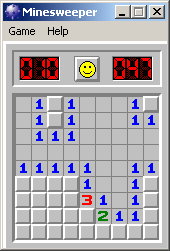
\includegraphics[width=\textwidth]{\CURPATH/1.png}
\caption{Random DAG}
\end{figure}

Arrows will represent information flow.
So a vertex (node) which has no incoming arrows to it (indegree=0), can be set to a random number.
Then we use topological sort to find dependencies between vertices.
Then we assign spreadsheet cell names to each vertex.
Then we generate random expression with random operations/numbers/cells to each cell,
with the use of information from topological sorted graph.

\input{\CURPATH/math}

Here is an output from \textit{Grid[]}:

\input{\CURPATH/grid.tex}

Using this script, I can generate random spreadsheet of $26 \cdot 500=13000$ cells,
which seems to be processed by Z3 in couple of seconds.

\subsubsection{The files}

The files, including Mathematica notebook: \url{.../spreadsheet}.


\subsection{Discrete tomography}

How computed tomography (CT scan) actually works?
A human body is bombarded by X-rays in various angles by X-ray tube in rotating torus.
X-ray detectors are also located in torus, and all the information is recorded.

Here is we can simulate simple tomograph.
An ``i'' character is rotating and will be ``enlighten'' at 4 angles.
Let's imagine, character is bombarded by X-ray tube at left.
All asterisks in each row is then summed and sum is "received" by X-ray detector at the right.

\begin{lstlisting}
WIDTH= 11 HEIGHT= 11
angle=(π/4)*0
    **      2
    **      2
            0
   ***      3
    **      2
    **      2
    **      2
    **      2
    **      2
   ****     4
            0
[2, 2, 0, 3, 2, 2, 2, 2, 2, 4, 0] ,
angle=(π/4)*1
            0
            0
  *         1
 **         2
    *       1
    **      2
     **     2
     ****   4
       *    1
      *     1
            0
[0, 0, 1, 2, 1, 2, 2, 4, 1, 1, 0] ,
angle=(π/4)*2
            0
            0
            0
            0
         *  1
** *******  9
** *******  9
   *     *  2
            0
            0
            0
[0, 0, 0, 0, 1, 9, 9, 2, 0, 0, 0] ,
angle=(π/4)*3
            0
            0
       *    1
       **   2
      ** *  3
     ***    3
    **      2
            0
  **        2
   *        1
            0
[0, 0, 1, 2, 3, 3, 2, 0, 2, 1, 0] ,
\end{lstlisting}

( The source code: \url{.../gen.py} )

All we got from our toy-level tomograph is 4 vectors, these are sums of all asterisks in rows for 4 angles:

\begin{lstlisting}
[2, 2, 0, 3, 2, 2, 2, 2, 2, 4, 0] ,
[0, 0, 1, 2, 1, 2, 2, 4, 1, 1, 0] ,
[0, 0, 0, 0, 1, 9, 9, 2, 0, 0, 0] ,
[0, 0, 1, 2, 3, 3, 2, 0, 2, 1, 0] ,
\end{lstlisting}

How do we recover initial image?
We are going to represent 11*11 matrix, where sum of each row must be equal to some value we already know.
Then we rotate matrix, and do this again.

For the first matrix, the system of equations looks like that (we put there a values from the first vector):

\begin{lstlisting}
C1,1 + C1,2 + C1,3 + ... + C1,11 =      2
C2,1 + C2,2 + C2,3 + ... + C2,11 =      2

...

C10,1 + C10,2 + C10,3 + ... + C10,11 =  4
C11,1 + C11,2 + C11,3 + ... + C11,11 =  0
\end{lstlisting}

We also build similar systems of equations for each angle.

The ``rotate'' function has been taken from the generation program, because, due to Python's dynamic typization nature,
it's not important for the function to what operate on:
strings, characters, or Z3 variable instances, so it works very well for all of them.

\lstinputlisting[style=custompy]{equations/tomo/solve.py}

( The source code: \url{...tomo/solve.py} )

That works:

\begin{lstlisting}
% python solve.py
sat
    **
    **

   ***
    **
    **
    **
    **
    **
   ****
\end{lstlisting}

In other words, all SMT-solver does here is solving a system of equations.

So, 4 angles are enough.
What if we could use only 3 angles?

\begin{lstlisting}
WIDTH= 11 HEIGHT= 11
angle=(π/3)*0
    **      2
    **      2
            0
   ***      3
    **      2
    **      2
    **      2
    **      2
    **      2
   ****     4
            0
[2, 2, 0, 3, 2, 2, 2, 2, 2, 4, 0] ,
angle=(π/3)*1
            0
            0
            0
 **         2
 **         2
   ***      3
     ****   4
       **   2
       *    1
            0
            0
[0, 0, 0, 2, 2, 3, 4, 2, 1, 0, 0] ,
angle=(π/3)*2
            0
            0
            0
       **   2
       **   2
     *****  5
    **      2
 **         2
  *         1
            0
            0
[0, 0, 0, 2, 2, 5, 2, 2, 1, 0, 0] ,
\end{lstlisting}

No, it's not enough:

\begin{lstlisting}
% time python solve3.py
sat
 *  *
    **

     * **
   **
   *  *
    **
     *   *
*   *
   ****
\end{lstlisting}

However, the result is correct, but only 3 vectors allows too many possible ``initial images'',
and Z3 SMT-solver finds first.

Further reading:
\url{https://en.wikipedia.org/wiki/Discrete_tomography},
\url{https://en.wikipedia.org/wiki/2-satisfiability#Discrete_tomography}.


\subsection{Cribbage}

I've found this problem in the Ronald L. Graham, Donald E. Knuth, Oren Patashnik -- ``Concrete Mathematics'' book:

\begin{framed}
\begin{quotation}
Cribbage players have long been aware that 15 = 7 + 8 = 4 + 5 + 6 =
1 + 2 + 3 + 4 + 5 . Find the number of ways to represent 1050 as a sum of
consecutive positive integers. (The trivial representation `1050' by itself
counts as one way; thus there are four, not three, ways to represent 15
as a sum of consecutive positive integers. Incidentally, a knowledge of
cribbage rules is of no use in this problem.)
\end{quotation}
\end{framed}

My solution:

\lstinputlisting{equations/cribbage/cribbage.py}

The result:

\begin{lstlisting}
(3 terms) 349 + ... + 351 == 1050
(4 terms) 261 + ... + 264 == 1050
(5 terms) 208 + ... + 212 == 1050
(7 terms) 147 + ... + 153 == 1050
(12 terms) 82 + ... + 93 == 1050
(15 terms) 63 + ... + 77 == 1050
(20 terms) 43 + ... + 62 == 1050
(21 terms) 40 + ... + 60 == 1050
(25 terms) 30 + ... + 54 == 1050
(28 terms) 24 + ... + 51 == 1050
(35 terms) 13 + ... + 47 == 1050
\end{lstlisting}


% TODO use MK85
\subsection{Solving Problem Euler 31: ``Coin sums''}

\begin{framed}
\begin{quotation}
In England the currency is made up of pound, £, and pence, p, and there are eight coins in general circulation:

1p, 2p, 5p, 10p, 20p, 50p, £1 (100p) and £2 (200p).
It is possible to make £2 in the following way:

1£1 + 150p + 220p + 15p + 12p + 31p
How many different ways can £2 be made using any number of coins?
\end{quotation}
\end{framed}
( \href{http://projecteuler.net/problem=31}{Problem Euler 31 --- Coin sums} )

\label{SMTEnumerate}
Using Z3 for solving this is overkill, and also slow, but nevertheless, it works, showing all possible solutions as well.
The piece of code for blocking already found solution and search for next, and thus, counting all solutions, was taken from Stack Overflow answer
\footnote{\url{http://stackoverflow.com/questions/11867611/z3py-checking-all-solutions-for-equation}, 
another question: \url{http://stackoverflow.com/questions/13395391/z3-finding-all-satisfying-models}}.
This is also called ``model counting''.
Constraints like ``a>=0'' must be present, because Z3 solver will find solutions with negative numbers.

\lstinputlisting[style=custompy]{equations/pe31/pe31.py}

Works very slow, and this is what it produces:

\begin{lstlisting}
[h = 0, g = 0, f = 0, e = 0, d = 0, c = 0, b = 0, a = 200]
[f = 1, b = 5, a = 0, d = 1, g = 1, h = 0, c = 2, e = 1]
[f = 0, b = 1, a = 153, d = 0, g = 0, h = 0, c = 1, e = 2]
...
[f = 0, b = 31, a = 33, d = 2, g = 0, h = 0, c = 17, e = 0]
[f = 0, b = 30, a = 35, d = 2, g = 0, h = 0, c = 17, e = 0]
[f = 0, b = 5, a = 50, d = 2, g = 0, h = 0, c = 24, e = 0]
\end{lstlisting}

73682 results in total.

\subsection{Exercise 15 from TAOCP ``7.1.3 Bitwise tricks and techniques''}

\renewcommand{\CURPATH}{equations/TAOCP_7_1_3_exercise_15}

Page 53 from the fasc1a.ps, or: \url{http://www.cs.utsa.edu/~wagner/knuth/fasc1a.pdf}

\begin{figure}[H]
\centering
\frame{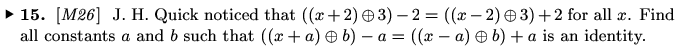
\includegraphics[scale=0.6]{\CURPATH/page53.png}}
\caption{Page 53}
\end{figure}

Soltuion:

\lstinputlisting[style=custompy]{\CURPATH/exercise_15.py}

For 4-bit bitvectors:

\begin{lstlisting}

...

[b = 7, a = 0]
[b = 6, a = 8]
[b = 7, a = 8]
[b = 6, a = 12]
[b = 7, a = 12]
[b = 12, a = 0]
[b = 13, a = 0]
[b = 12, a = 8]
[b = 13, a = 8]
[b = 12, a = 4]
[b = 13, a = 4]
[b = 12, a = 12]
[b = 13, a = 12]
[b = 14, a = 0]
[b = 15, a = 0]
[b = 14, a = 4]
[b = 15, a = 4]
[b = 14, a = 8]
[b = 15, a = 8]
[b = 14, a = 12]
[b = 15, a = 12]
results total= 128
\end{lstlisting}


\section{Generating de Bruijn sequences using Z3}
\label{DeBruijnZ3}

(\MathForProg has a part about de Bruijn sequences.)

\renewcommand{\CURPATH}{equations/de_bruijn_SMT}

The following piece of quite esoteric code calculates number of leading zero bits
\footnote{\url{https://en.wikipedia.org/wiki/Find_first_set}}:

\begin{lstlisting}
int v[64]=
	{ -1,31, 8,30, -1, 7,-1,-1, 29,-1,26, 6, -1,-1, 2,-1,
	  -1,28,-1,-1, -1,19,25,-1, 5,-1,17,-1, 23,14, 1,-1,
	   9,-1,-1,-1, 27,-1, 3,-1, -1,-1,20,-1, 18,24,15,10,
	  -1,-1, 4,-1, 21,-1,16,11, -1,22,-1,12, 13,-1, 0,-1 };

int LZCNT(uint32_t x)
{
    x |= x >> 1;
    x |= x >> 2;
    x |= x >> 4;
    x |= x >> 8;
    x |= x >> 16;
    x *= 0x4badf0d;
    return v[x >> 26];
}
\end{lstlisting}

(This is usually done using simpler algorithm, but it will contain conditional jumps, which is bad for
CPUs starting at RISC. There are no conditional jumps in this algorithm.)

The magic number used here is called \emph{de Bruijn sequence},
and I once used bruteforce to find it (one of the results was \emph{0x4badf0d}, which is used here).
But what if we need magic number for 64-bit values?
Bruteforce is not an option here.

If you already read about these sequences in my blog or in other sources,
you can see that the 32-bit magic number is a number consisting
of 5-bit overlapping chunks, and all chunks must be unique, i.e., must not be repeating.

For 64-bit magic number, these are 6-bit overlapping chunks.

To find the magic number, one can find a Hamiltonian path of a de Bruijn graph.
But I've found that Z3 is also can do this, though, overkill, but this is more illustrative.

\lstinputlisting[style=custompy]{\CURPATH/64.py}

We just enumerate all overlapping 6-bit chunks and tell Z3 that they must be unique (see \TT{Distinct}).
Output:

\lstinputlisting{\CURPATH/output.txt}

Overlapping chunks are clearly visible.
So the magic number is \emph{0x79c52dd0991abf60}.
Let's check:

\lstinputlisting[style=customc]{\CURPATH/64.c}

That works!


\subsection{Solving the $x^y=19487171$ equation}

Find x,y for $x^y=19487171$.
The correct result x=11, y=7.
It's like \url{http://reference.wolfram.com/language/ref/Surd.html}.

The non-standard function \verb|bvmul_no_overflow| is used here. it behaves like bvmul, but high part is forced to be zero.
This is not like most programming languages and CPUs do multiplication
(the result there is modulo $2^n$, where $n$ is width of CPU register).
However, thus it's simpler for me to write this all without adding additional \verb|zero_extend| function.

\lstinputlisting[style=customsmt]{equations/surd/surd.smt}

\begin{lstlisting}[caption=The solution]
(model
        (define-fun x () (_ BitVec 32) (_ bv11 32)) ; 0xb
        (define-fun y () (_ BitVec 4) (_ bv7 4)) ; 0x7
        (define-fun out () (_ BitVec 32) (_ bv19487171 32)) ; 0x12959c3
)
\end{lstlisting}



}
\RU{\section{Уравнения}

% subsections:
\subsection{Решение XKCD 287}
\label{XkcdILP}

\begin{figure}[H]
\centering
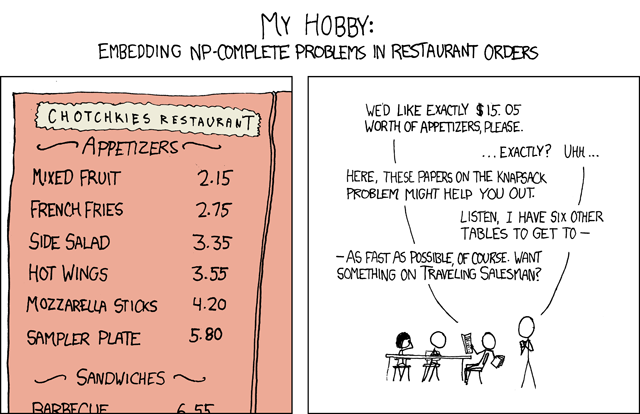
\includegraphics[scale=7]{equations/xkcd287/np_complete.png}
\caption{xkcd \#287}
\end{figure}

( \url{https://www.xkcd.com/287/} )

Вот перевод на русский, но с другими ценами:

\begin{figure}[H]
\centering
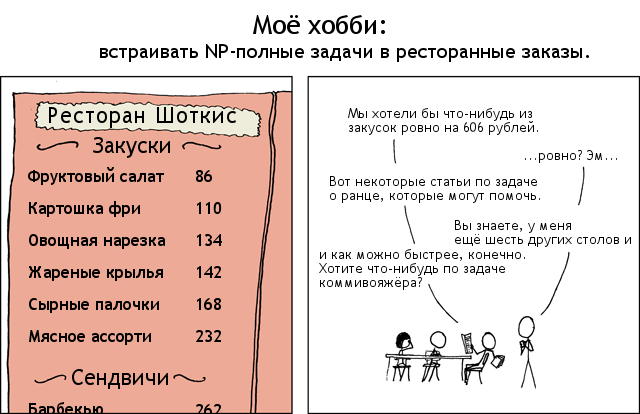
\includegraphics[scale=7]{equations/xkcd287/287_v1.png}
\caption{xkcd \#287}
\end{figure}

( \url{https://xkcd.ru/287/} )

(Но мы всё равно будем ориентироваться на цены из оригинальной англоязычной версии.)

Задача в том, чтобы решить следующее уравнение:
$2.15a + 2.75b + 3.35c + 3.55d + 4.20e + 5.80f == 15.05$,
где a..f это целочисленные.
Так что это линейное диофантово уравнение.

\lstinputlisting{equations/xkcd287/xkcd287_MK85.py}

( Исходный код: \url{https://github.com/DennisYurichev/.../xkcd287_MK85.py} )

Тут только 2 решения:

\begin{lstlisting}
{'a': 7, 'c': 0, 'b': 0, 'e': 0, 'd': 0, 'f': 0}
{'a': 1, 'c': 0, 'b': 0, 'e': 0, 'd': 2, 'f': 1}
\end{lstlisting}

Wolfram Mathematica тоже может решить это уравнение:

\begin{lstlisting}
In[]:= FindInstance[2.15 a + 2.75 b + 3.35 c + 3.55 d + 4.20 e + 5.80 f == 15.05 && 
	a >= 0 && b >= 0 && c >= 0 && d >= 0  && e >= 0 && f >= 0, 
	{a, b, c, d, e, f}, Integers, 1000]

Out[]= {{a -> 1, b -> 0, c -> 0, d -> 2, e -> 0, f -> 1},
	{a -> 7, b -> 0, c -> 0, d -> 0, e -> 0, f -> 0}}
\end{lstlisting}

1000 означает ``найти максимум 1000 решений'', но находится только 2.
См.также: \url{http://reference.wolfram.com/language/ref/FindInstance.html}.\\
\\
Другие способы решения:
\url{https://stackoverflow.com/questions/141779/solving-the-np-complete-problem-in-xkcd},
\url{http://www.explainxkcd.com/wiki/index.php/287:_NP-Complete}.

Решение используя Z3: \url{https://github.com/DennisYurichev/.../xkcd287_Z3.py} )

\subsection{XKCD 287 в формате SMT-LIB 2.x}

\lstinputlisting{equations/xkcd287/xkcd287.smt}


%\input{equations/2017_AMC_12A_Problem_2_RU}
%\section{Развлекательная математика и головоломки}

\input{puzzles/sudoku/main_RU}
\input{puzzles/zebra/main_RU}
\input{puzzles/pipe/main_RU}
\input{puzzles/rubik2/failed_SMT/main_RU}
\input{puzzles/rubik2/SAT/main_RU}
\input{puzzles/rubik3/one_face_SMT/main_RU}
%\input{puzzles/numberlink/main_RU}
%\input{puzzles/two_parks_RU}
\input{puzzles/alphametics/main_RU}
%\input{puzzles/2015_AIME_II_Problems_12_RU}
%\input{puzzles/fred/main_RU}
%\input{puzzles/MC/main_RU}
%\input{puzzles/coin_flip/main_RU}
%\input{puzzles/Mock_AIME_2_2006-2007_Problem_8_RU}
%\input{puzzles/2012_AIME_I_Problems_1_RU}
%\input{puzzles/keypad_RU}


\subsection{Школьное уравнение}

Снова вернемся к школьной системы уравнений из (\ref{eq2_SMT}).

Заставим KLEE найти путь, где все констрайнты будут удовлетворены:

\lstinputlisting[style=customc]{equations/KLEE_eq/klee_eq2.c}

\begin{lstlisting}
% clang -emit-llvm -c -g klee_eq.c
...

% klee klee_eq.bc
KLEE: output directory is "/home/klee/klee-out-93"
KLEE: WARNING: undefined reference to function: klee_assert
KLEE: WARNING ONCE: calling external: klee_assert(0)
KLEE: ERROR: /home/klee/klee_eq.c:18: failed external call: klee_assert
KLEE: NOTE: now ignoring this error at this location

KLEE: done: total instructions = 32
KLEE: done: completed paths = 1
KLEE: done: generated tests = 1
\end{lstlisting}

Найдем, где сработал \TT{klee\_assert()}:

\begin{lstlisting}
% ls klee-last | grep err
test000001.external.err

% ktest-tool --write-ints klee-last/test000001.ktest
ktest file : 'klee-last/test000001.ktest'
args       : ['klee_eq.bc']
num objects: 3
object    0: name: b'circle'
object    0: size: 4
object    0: data: 5
object    1: name: b'square'
object    1: size: 4
object    1: data: 2
object    2: name: b'triangle'
object    2: size: 4
object    2: data: 1
\end{lstlisting}

Это действительно правильное решение системы уравнений.

В KLEE есть \textit{intrinsic} \TT{klee\_assume()} который указывает KLEE обрезать путь, если некоторый констрайнт не удовлетворен.
Так что мы можем переписать наш пример в более чистом виде:

\lstinputlisting[style=customc]{equations/KLEE_eq/klee_eq2.c}


\subsection{Взлом Сапёра при помощи Z3 SMT-солвера}
\label{minesweeper_SMT}

\renewcommand{\CURPATH}{equations/minesweeper_SMT}

Для тех кто не очень хорошо играет в Сапёр (как я), можно предсказывать расположение бомб без помощи отладчика.

Вот я где-то нажал и я вижу пустые ячейки и ячейки с количеством ``соседей'':

\begin{figure}[H]
\centering
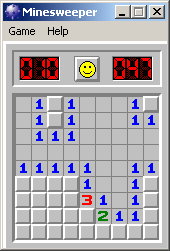
\includegraphics[scale=0.75]{\CURPATH/1.png}
\end{figure}

Что у нас тут, на самом деле? Скрытые ячейки, пустые ячейки (где нет бомб) и пустые ячейки с числами,
показывающими, сколько рядом бомб.

\subsubsection{Метод}

Вот что мы можем сделать: мы будем пытаться расположить бомбу во всех возможных скрытых ячейках и спрашивать Z3 SMT-солвер,
можно ли доказать тот факт, что бомба не может быть расположена там.

Посмотрите на этот фрагмент. "?" означает скрытую ячейку, "." пустую ячейку, число это число соседей.

\begin{center}
\begin{tabular}{ | c | c | c | c | }
\hline
 & C1 & C2 & C3 \\
\hline
R1 & ? & ? & ? \\
\hline
R2 & ? & 3 & . \\
\hline
R3 & ? & 1 & . \\
\hline
\end{tabular}
\end{center}

Так что здесь 5 скрытых ячеек.
Будем проверят каждую скрытую ячейку, располагая там бомбу.
Начинаем с верхней/левой ячейки:

\begin{center}
\begin{tabular}{ | c | c | c | c | }
\hline
 & C1 & C2 & C3 \\
\hline
R1 & * & ? & ? \\
\hline
R2 & ? & 3 & . \\
\hline
R3 & ? & 1 & . \\
\hline
\end{tabular}
\end{center}

Затем мы пытаемся решить следующую систему уравнений (\textit{RrCc} это ячейка из ряда $r$ и столбца $c$):

\begin{itemize}
\item R1C2+R2C1+R2C2=1                               (потому что мы расположили бомбу на R1C1)	
\item R2C1+R2C2+R3C1=1                               (потому что у нас "1" на R3C2)	
\item R1C1+R1C2+R1C3+R2C1+R2C2+R2C3+R3C1+R3C2+R3C3=3 (потому что у нас "3" на R2C2)	
\item R1C2+R1C3+R2C2+R2C3+R3C2+R3C3=0                (потому что у нас "." на R2C3)	
\item R2C2+R2C3+R3C2+R3C3=0                          (потому что у нас "." на R3C3)
\end{itemize}

Как выясняется, эта система уравнений решаема, так что в этой ячейке может быть бомба.
И это информация нам не интересна, так как мы хотим найти ячейки, на которые можно свободно кликать.
И мы попробуем другую.
И если уравнение будет нерешаемо, это будет означать, что там не может быть бомбы, и можно кликнуть.

\subsubsection{Код}

\lstinputlisting{\CURPATH/minesweeper_solver.py}

Этот код самодокументирован и его легко понять без объяснений.
Граница нужна по той же причине, почему реализации игры "Жизнь" Конвея также имеют границу (чтобы сделать
ф-цию для вычисления проще).
Когда мы знаем что в ячейке нет бомбы, мы вписываем туда ноль.
Когда мы знаем количество соседей, мы добавляем констрайнт, снова, как и в игре "Жизнь": количество соседей
должно равняться числу, которое мы увидели в Сапёре.
Затем мы располагаем бомбу где-нибудь и проверяем.

Запускаем:

\begin{lstlisting}
row=1 col=3, unsat!
row=6 col=2, unsat!
row=6 col=3, unsat!
row=7 col=4, unsat!
row=7 col=9, unsat!
row=8 col=9, unsat!
\end{lstlisting}

Это ячейки, которые можно кликать без боязни, что я и сделал:

\begin{figure}[H]
\centering
\includegraphics[scale=0.75]{\CURPATH/2.png}
\end{figure}

Теперь у нас больше информации и мы обновляем входное условие:

\begin{lstlisting}
known=[
"01110001?",
"01?100011",
"011100000",
"000000000",
"111110011",
"?11?1001?",
"???331011",
"?????2110",
"???????10"]
\end{lstlisting}

Запускаю снова:

\begin{lstlisting}
row=7 col=1, unsat!
row=7 col=2, unsat!
row=7 col=3, unsat!
row=8 col=3, unsat!
row=9 col=5, unsat!
row=9 col=6, unsat!
\end{lstlisting}

Нажимаю на эти ячейки снова:

\begin{figure}[H]
\centering
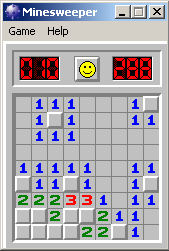
\includegraphics[scale=0.75]{\CURPATH/3.png}
\end{figure}

Обновляю снова:

\begin{lstlisting}
known=[
"01110001?",
"01?100011",
"011100000",
"000000000",
"111110011",
"?11?1001?",
"222331011",
"??2??2110",
"????22?10"]
\end{lstlisting}

\begin{lstlisting}
row=8 col=2, unsat!
row=9 col=4, unsat!
\end{lstlisting}

\begin{figure}[H]
\centering
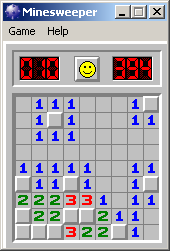
\includegraphics[scale=0.75]{\CURPATH/4.png}
\end{figure}

Последнее обновление:

\begin{lstlisting}
known=[
"01110001?",
"01?100011",
"011100000",
"000000000",
"111110011",
"?11?1001?",
"222331011",
"?22??2110",
"???322?10"]
\end{lstlisting}

\dots последний результат:

\begin{lstlisting}
row=9 col=1, unsat!
row=9 col=2, unsat!
\end{lstlisting}

Вуаля!

\begin{figure}[H]
\centering
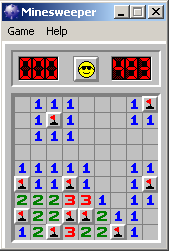
\includegraphics[scale=0.75]{\CURPATH/5.png}
\end{figure}

Исходный код: \url{.../minesweeper_solver.py}.

Обсуждение на HN: \url{https://news.ycombinator.com/item?id=13797375}.


\subsection{Взлом Сапёра при помощи SAT}
\label{minesweeper_SAT}

\subsubsection{Простая ф-ция подсчета бит (\textit{population count})}

Прежде всего, нам нужно как считать количество соседних бомб.
Ф-ция подсчета та же, что и ф-ция подсчета бит (\textit{population count}).

Мы можем создать \ac{CNF}-выражение используя Wolfram Mathematica.
Это будет ф-ция, возвращающая \textit{True} если любые из двух бит 8-битного входа равняются \textit{True},
а остальные --- \textit{False}.
В начале, сделаем таблицу истинности для такой ф-ции:

\begin{lstlisting}
In[]:= tbl2 = 
 Table[PadLeft[IntegerDigits[i, 2], 8] -> 
   If[Equal[DigitCount[i, 2][[1]], 2], 1, 0], {i, 0, 255}]

Out[]= {{0, 0, 0, 0, 0, 0, 0, 0} -> 0, {0, 0, 0, 0, 0, 0, 0, 1} -> 0, 
{0, 0, 0, 0, 0, 0, 1, 0} -> 0, {0, 0, 0, 0, 0, 0, 1, 1} -> 1, 
{0, 0, 0, 0, 0, 1, 0, 0} -> 0, {0, 0, 0, 0, 0, 1, 0, 1} -> 1, 
{0, 0, 0, 0, 0, 1, 1, 0} -> 1, {0, 0, 0, 0, 0, 1, 1, 1} -> 0, 
{0, 0, 0, 0, 1, 0, 0, 0} -> 0, {0, 0, 0, 0, 1, 0, 0, 1} -> 1, 
{0, 0, 0, 0, 1, 0, 1, 0} -> 1, {0, 0, 0, 0, 1, 0, 1, 1} -> 0, 
...
{1, 1, 1, 1, 1, 0, 1, 0} -> 0, {1, 1, 1, 1, 1, 0, 1, 1} -> 0, 
{1, 1, 1, 1, 1, 1, 0, 0} -> 0, {1, 1, 1, 1, 1, 1, 0, 1} -> 0, 
{1, 1, 1, 1, 1, 1, 1, 0} -> 0, {1, 1, 1, 1, 1, 1, 1, 1} -> 0}
\end{lstlisting}

Теперь можем сделать \ac{CNF}-выражение используя эту таблицу истинности:

\begin{lstlisting}
In[]:= BooleanConvert[
 BooleanFunction[tbl2, {a, b, c, d, e, f, g, h}], "CNF"]

Out[]= (! a || ! b || ! c) && (! a || ! b || ! d) && (! a || ! 
    b || ! e) && (! a || ! b || ! f) && (! a || ! b || ! g) && (! 
    a || ! b || ! h) && (! a || ! c || ! d) && (! a || ! c || ! 
    e) && (! a || ! c || ! f) && (! a || ! c || ! g) && (! a || ! 
    c || ! h) && (! a || ! d || ! e) && (! a || ! d || ! f) && (! 
    a || ! d || ! g) && (! a || ! d || ! h) && (! a || ! e || ! 
    f) && (! a || ! e || ! g) && (! a || ! e || ! h) && (! a || ! 
    f || ! g) && (! a || ! f || ! h) && (! a || ! g || ! h) && (a || 
   b || c || d || e || f || g) && (a || b || c || d || e || f || 
   h) && (a || b || c || d || e || g || h) && (a || b || c || d || f ||
    g || h) && (a || b || c || e || f || g || h) && (a || b || d || 
   e || f || g || h) && (a || c || d || e || f || g || 
   h) && (! b || ! c || ! d) && (! b || ! c || ! e) && (! b || ! 
    c || ! f) && (! b || ! c || ! g) && (! b || ! c || ! h) && (! 
    b || ! d || ! e) && (! b || ! d || ! f) && (! b || ! d || ! 
    g) && (! b || ! d || ! h) && (! b || ! e || ! f) && (! b || ! 
    e || ! g) && (! b || ! e || ! h) && (! b || ! f || ! g) && (! 
    b || ! f || ! h) && (! b || ! g || ! h) && (b || c || d || e || 
   f || g || 
   h) && (! c || ! d || ! e) && (! c || ! d || ! f) && (! c || ! 
    d || ! g) && (! c || ! d || ! h) && (! c || ! e || ! f) && (! 
    c || ! e || ! g) && (! c || ! e || ! h) && (! c || ! f || ! 
    g) && (! c || ! f || ! h) && (! c || ! g || ! h) && (! d || ! 
    e || ! f) && (! d || ! e || ! g) && (! d || ! e || ! h) && (! 
    d || ! f || ! g) && (! d || ! f || ! h) && (! d || ! g || ! 
    h) && (! e || ! f || ! g) && (! e || ! f || ! h) && (! e || ! 
    g || ! h) && (! f || ! g || ! h)
\end{lstlisting}

Синтаксис такой же как и в Си/Си++
Проверим.

Я написал Питоновскую ф-цию для конвертирования вывода Mathematica в \ac{CNF}-файл, который можно подать на вход
SAT-солверу:

\lstinputlisting{SAT/minesweeper/tst.py}

Она заменяет переменные a/b/c/... на переданные имена переменных (1/2/3...), перерабатыает синтаксис, итд.
Вот результат:

\lstinputlisting{SAT/minesweeper/tst1.cnf}

Могу запустить:

\begin{lstlisting}
% minisat -verb=0 tst1.cnf results.txt
SATISFIABLE

% cat results.txt
SAT
1 -2 -3 -4 -5 -6 -7 8 0
\end{lstlisting}

Имя переменной в результате без знака минуса, это \textit{True}.
Имя переменной со знаком минус, это \textit{False}.
Мы здесь видим только две переменных \textit{True}: 1 и 8.
Это действительно корректно: солвер MiniSat нашел условие, для которого наша ф-ция возвращает \textit{True}.
Ноль в конце это просто терминирующий символ, который ничего не означает.

Мы можем попросить MiniSat найти еще одно решение, добавив текущее решение во входной CNF-файл,
но где все переменные инвертированы:

\begin{lstlisting}
...
-5 -6 -8 0
-5 -7 -8 0
-6 -7 -8 0
-1 2 3 4 5 6 7 -8 0
\end{lstlisting}

В обычном русском языке, это означает ``дайте ЛЮБОЕ решение, которые удовлетворяет все клозы, но также не равно
последнему клозу, которое мы только что добавили''.

MiniSat, действительно, находит еще одно решение, и снова, только с двумя переменными, равными \textit{True}:

\begin{lstlisting}
% minisat -verb=0 tst2.cnf results.txt
SATISFIABLE

% cat results.txt
SAT
1 2 -3 -4 -5 -6 -7 -8 0
\end{lstlisting}

Кстати, ф-ция \textit{population count} для 8-и соседей (POPCNT8) в CNF-форме, самая простая:

\begin{lstlisting}
a&&b&&c&&d&&e&&f&&g&&h
\end{lstlisting}

Действительно: она истинна, если все 8 входных бит тоже истинны.

Ф-ция для отсутствия соседей (POPCNT0) тоже очень простая:

\begin{lstlisting}
!a&&!b&&!c&&!d&&!e&&!f&&!g&&!h
\end{lstlisting}

Это означает, что она вернет \textit{True}, если все входные переменные \textit{False}.

Кстати, ф-ция POPCNT1 тоже простая:

\begin{lstlisting}
(!a||!b)&&(!a||!c)&&(!a||!d)&&(!a||!e)&&(!a||!f)&&(!a||!g)&&(!a||!h)&&(a||b||c||d||e||f||g||h)&&
(!b||!c)&&(!b||!d)&&(!b||!e)&&(!b||!f)&&(!b||!g)&&(!b||!h)&&(!c||!d)&&(!c||!e)&&(!c||!f)&&(!c||!g)&&
(!c||!h)&&(!d||!e)&&(!d||!f)&&(!d||!g)&&(!d||!h)&&(!e||!f)&&(!e||!g)&&(!e||!h)&&(!f||!g)&&(!f||!h)&&(!g||!h)
\end{lstlisting}

Здесь просто перечисление всех возможных пар 8-и переменных
(a/b, a/c, a/d, итд), что подразумевает: не должно присутствовать одновременно двух бит в каждой возможной паре.
И еще один клоз: ``(a||b||c||d||e||f||g||h)'', что подразумевает: минимум один бит должен присутствовать
среди 8-и переменных.

И да, вы можете использовать Mathematica для поиска \ac{CNF}-выражения для любой другой таблицы истинности.

\subsubsection{Сапёр}

Теперь можем использовать Mathematica для генерации всех ф-ций \textit{population count} для количества соседей 0..8.

Для Сапёра с матрицей $9 \cdot 9$ включая невидимую рамку, здесь будет $11 \cdot 11=121$ переменных,
связанных с матрицей Сапёра вот так:

\begin{lstlisting}
 1    2   3   4   5   6   7   8   9  10  11
12   13  14  15  16  17  18  19  20  21  22
23   24  25  26  27  28  29  30  31  32  33
34   35  36  37  38  39  40  41  42  43  44

...

100 101 102 103 104 105 106 107 108 109 110
111 112 113 114 115 116 117 118 119 120 121
\end{lstlisting}

Потом мы пишем Питоновский скрипт, складывающий все ф-ции \textit{population count}:
каждая ф-ция для каждого известного числа соседей (число на поле Сапёра).
Каждая ф-ция POPCNTx() берет на вход список переменных и выдает список клозов, которые будут добавлены
в итоговый \ac{CNF}-файл.

Что до пустых клеток, мы тоже добавляем их как клозы, но со знаком минус, что означает, что переменная
должна быть \textit{False}.
А когда мы пытаемся поместить бомбу, мы добавляем её переменную как клоз без знака минуса, что означает
что переменная должна быть \textit{True}.

Затем запускаем внешний процесс minisat.
Всё что нам от него нужно, это код возврата.
Если входной \ac{CNF} это \TT{UNSAT}, он возвращает 20:

Мы также используем здесь информацию из предыдущего решения Сапёра: \ref{minesweeper_SMT}.

\lstinputlisting{SAT/minesweeper/minesweeper_SAT.py}

( \url{https://github.com/DennisYurichev/SAT_SMT_article/blob/master/SAT/minesweeper/minesweeper_SAT.py} ) \\
\\
Выходной \ac{CNF}-файл большой, вплоть до $\approx 2000$ клозов, и даже больше, вот, например: \url{https://github.com/DennisYurichev/SAT_SMT_article/blob/master/SAT/minesweeper/sample.cnf}.

Так или иначе, это работает так же, как мой предыдущий скрипт для Z3Py:

\begin{lstlisting}
row=1, col=3, unsat!
row=6, col=2, unsat!
row=6, col=3, unsat!
row=7, col=4, unsat!
row=7, col=9, unsat!
row=8, col=9, unsat!
\end{lstlisting}

\dots но работает намного быстрее, даже учитывая запуск внешней программы.
Вероятно, версию для Z3Py можно было бы оптимизировать получше?

Файлы, включая файл для Wolfram Mathematica: \url{https://github.com/DennisYurichev/SAT_SMT_article/tree/master/SAT/minesweeper}.


\subsection{Взлом \ac{LCG} при помощи Z3}

У \ac{LCG} есть хорошо известные слабости
\footnote{\url{http://en.wikipedia.org/wiki/Linear_congruential_generator\#Advantages_and_disadvantages_of_LCGs},
\url{http://www.reteam.org/papers/e59.pdf},
\url{http://stackoverflow.com/questions/8569113/why-1103515245-is-used-in-rand/8574774\#8574774}},
но посмотрим, можно ли его взломать напрямую, без специальных знаний.
Мы определим все связи между состояниями LCG в терминах Z3.
Вот тестовая программа:

\begin{lstlisting}
#include <stdlib.h>
#include <stdio.h>
#include <time.h>

int main()
{
	int i;

	srand(time(NULL));

	for (i=0; i<10; i++)
		printf ("%d\n", rand()%100);
};
\end{lstlisting}

Она выдает 10 псевдослучайных чисел в пределах 0..99:

\begin{lstlisting}
37
29
74
95
98
40
23
58
61
17
\end{lstlisting}

Скажем, мы наблюдаем только 8 из этих чисел (от 29 до 61) и нам нужно предсказать следующее (17) и/или предыдущее (37).

Программа скомпилирована в MSVC 2013 (я выбрал его потому что тут LCG проще чем в Glib):

\begin{lstlisting}
.text:0040112E rand            proc near
.text:0040112E                 call    __getptd
.text:00401133                 imul    ecx, [eax+0x14], 214013
.text:0040113A                 add     ecx, 2531011
.text:00401140                 mov     [eax+14h], ecx
.text:00401143                 shr     ecx, 16
.text:00401146                 and     ecx, 7FFFh
.text:0040114C                 mov     eax, ecx
.text:0040114E                 retn
.text:0040114E rand            endp
\end{lstlisting}

Определим \ac{LCG} в Z3Py:

\begin{lstlisting}
#!/usr/bin/python
from z3 import *

output_prev = BitVec('output_prev', 32)
state1 = BitVec('state1', 32)
state2 = BitVec('state2', 32)
state3 = BitVec('state3', 32)
state4 = BitVec('state4', 32)
state5 = BitVec('state5', 32)
state6 = BitVec('state6', 32)
state7 = BitVec('state7', 32)
state8 = BitVec('state8', 32)
state9 = BitVec('state9', 32)
state10 = BitVec('state10', 32)
output_next = BitVec('output_next', 32)

s = Solver()

s.add(state2 == state1*214013+2531011)
s.add(state3 == state2*214013+2531011)
s.add(state4 == state3*214013+2531011)
s.add(state5 == state4*214013+2531011)
s.add(state6 == state5*214013+2531011)
s.add(state7 == state6*214013+2531011)
s.add(state8 == state7*214013+2531011)
s.add(state9 == state8*214013+2531011)
s.add(state10 == state9*214013+2531011)

s.add(output_prev==URem((state1>>16)&0x7FFF,100))
s.add(URem((state2>>16)&0x7FFF,100)==29)
s.add(URem((state3>>16)&0x7FFF,100)==74)
s.add(URem((state4>>16)&0x7FFF,100)==95)
s.add(URem((state5>>16)&0x7FFF,100)==98)
s.add(URem((state6>>16)&0x7FFF,100)==40)
s.add(URem((state7>>16)&0x7FFF,100)==23)
s.add(URem((state8>>16)&0x7FFF,100)==58)
s.add(URem((state9>>16)&0x7FFF,100)==61)
s.add(output_next==URem((state10>>16)&0x7FFF,100))

print(s.check())
print(s.model())
\end{lstlisting}

\textit{URem} означает \textit{unsigned remainder} (беззнаковый остаток от деления).
Какое-то время работает и выдает корректный результат!

\begin{lstlisting}
sat
[state3 = 2276903645,
 state4 = 1467740716,
 state5 = 3163191359,
 state7 = 4108542129,
 state8 = 2839445680,
 state2 = 998088354,
 state6 = 4214551046,
 state1 = 1791599627,
 state9 = 548002995,
 output_next = 17,
 output_prev = 37,
 state10 = 1390515370]
\end{lstlisting}

Я добавил $\approx 10$ состояний, чтобы быть уверенным, что результат будет верным.
Но так могло и не быть, в случае с меньшим количеством информации.

Это причина, по которой \ac{LCG} не предназначена для любых задач связанных с безопасностью.
Вот почему существуют криптостойкие генераторы псевдослучайных чисел:
они разработаны с защитой от такой простой атаки.
Ну, по крайней мере, если \ac{NSA} не вмешивается
\footnote{\url{https://en.wikipedia.org/wiki/Dual_EC_DRBG}}.

Токены вроде ``RSA SecurID'' можно рассматривать просто как \ac{CPRNG} с секретным изначальным состоянием (seed).
Они показыают псевдослучайное число каждую минуту, и сервер может его предсказать, потому что знает seed.
Представьте, если бы такой токен использовал \ac{LCG} --- взломать его было бы куда проще!


%\input{equations/LCG/2_RU}
% TODO translate


TODO translate!


\subsection{Пересчет упрощенной электронной таблицы используя Z3Py}

\renewcommand{\CURPATH}{equations/spreadsheet}

% TODO cite?
Есть неплохая задача\footnote{\url{http://thesz.livejournal.com/280784.html}}:
напишите программу для пересчета упрощенной электронной таблицы, вот как такой:

\lstinputlisting{\CURPATH/test1}

Результат должен быть такой:

\lstinputlisting{\CURPATH/test1_result}

Как выясняется, хотя это и слишком, но это может решить MK85 без всякого труда:

\lstinputlisting{\CURPATH/spreadsheet_MK85.py}

( \url{.../spreadsheet_MK85.py} )

Всё что мы делаем это создаем пачку переменных для каждой ячейки, с названиями 
A0, B1, итд, целочисленного типа.
Все они сохраняются в словаре \textit{cells[]}.
Ключ это строка.
Затем мы парсим все строки из ячеек и добавляем их в список констрайнтов, в случае числа в ячейке: \textit{A0=123},
либо, в случае выражения в ячейке: \textit{A0=B1+C2}.
Тут есть небольшая подготовка строк: строка вроде \textit{A0+B2} становится \textit{cells["A0"]+cells["B2"]}.

Затем строка обрабатыватся Питоновским методом \textit{eval()}, который очень опасен
\footnote{\url{http://stackoverflow.com/questions/1832940/is-using-eval-in-python-a-bad-practice}}:
представьте, если конечный пользователь добавить в ячейку строку с каким-нибудь другим выражением?
Тем не менее, это хорошо служит нашим целям, потому что это простейший способ передать строку с выражением в Z3.

\subsubsection{Z3}

Исходный код почти такой же:

\lstinputlisting{\CURPATH/spreadsheet_Z3_1.py}

( \url{...spreadsheet/spreadsheet_Z3_1.py} )

\subsubsection{Unsat core}

Теперь проблема: что если здесь есть циркулярная (круговая) зависимость? Например:

\lstinputlisting{\CURPATH/test_circular}

Первые две ячейки последнего ряда (C0 и C1) завязаны друг на друга.
Наша программа просто скажет ``unsat'', означая, что она не смогла удовлетворить все констрайнты.
Мы не можем это использовать как сообщение об ошибке для конечного пользователя, потому что от него мало толка.

Хотя, мы можем вытащить \textit{unsat core}, т.е., список переменных, которые для Z3 являются конфликтующими.

\begin{lstlisting}
...
s=Solver()
s.set(unsat_core=True)
...
        # add constraint:
        s.assert_and_track(e, coord_to_name(cur_R, cur_C))
...
if result=="sat":
...
else:
    print s.unsat_core()
\end{lstlisting}

( \url{.../spreadsheet_Z3_2.py} )

Нам нужно явно включить поддержку unsat core и использовать \textit{assert\_and\_track()} вместо метода \textit{add()},
потому что эта возможность замедляет весь процесс, и по умолчанию отключена.
Это работает:

\begin{lstlisting}
 % python 2.py test_circular
unsat
[C0, C1]
\end{lstlisting}

Вероятно, эти переменные могут быть удалены из двухмерного массива, маркированы как \textit{unresolved},
и вся таблица могла бы быть пересчитанной заново.

\subsubsection{Нагрузочное тестирование}

Как сгенерировать большую случайную электронную таблицу?
Вот что мы можем сделать.
В начале создаем случайный \ac{DAG}, как вот этот:

\begin{figure}[H]
\centering
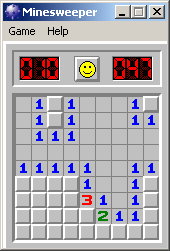
\includegraphics[width=\textwidth]{\CURPATH/1.png}
\caption{Случайный DAG}
\end{figure}

Стрелки определяют потоки информации.
Так что узел графа, который не имеет входящих стрелок (indegree=0), может быть установлен в случайное число.
Затем мы используем топологическую сортировку для поиска зависимостей между узлами графа.
Затем мы назначаем имена ячеек каждому узлу.
Затем мы генерируем случайное выражение со случайными операциями/числами/ячейками, используя информацию
полученную из топологически отсортированного графа.

\input{\CURPATH/math}

Вот вывод ф-ции \textit{Grid[]}:

\input{\CURPATH/grid.tex}

Используя этот скрипт, я могу сгенерировать случайную электронную таблицу из $26 \cdot 500=13000$ ячеек,
которая затем обрабатывается Z3 несколько секунд.

\subsubsection{Файлы}

Файлы, включая файл для Mathematica: \url{.../spreadsheet}.


\subsection{Дискретная томография}

Как компьютерная томография (КТ) вообще работает?
Тело человека бомбардируется рентгеновскими лучами под разными углами во вращающемся торе.
Детекторы излучения также находятся в торе и вся информация записывается.

Мы тут можем симулировать простой томограф.
Символ ``i'' вращается и будет ``просвечен'' под 4-я углами.
Представим что символ бомбардируется рентгеновскими лучами слева.
Все звездочки в каждом ряду суммируются и сумма ``принимается'' рентгеновскими детекторами справа.

\begin{lstlisting}
WIDTH= 11 HEIGHT= 11
angle=(π/4)*0
    **      2
    **      2
            0
   ***      3
    **      2
    **      2
    **      2
    **      2
    **      2
   ****     4
            0
[2, 2, 0, 3, 2, 2, 2, 2, 2, 4, 0] ,
angle=(π/4)*1
            0
            0
  *         1
 **         2
    *       1
    **      2
     **     2
     ****   4
       *    1
      *     1
            0
[0, 0, 1, 2, 1, 2, 2, 4, 1, 1, 0] ,
angle=(π/4)*2
            0
            0
            0
            0
         *  1
** *******  9
** *******  9
   *     *  2
            0
            0
            0
[0, 0, 0, 0, 1, 9, 9, 2, 0, 0, 0] ,
angle=(π/4)*3
            0
            0
       *    1
       **   2
      ** *  3
     ***    3
    **      2
            0
  **        2
   *        1
            0
[0, 0, 1, 2, 3, 3, 2, 0, 2, 1, 0] ,
\end{lstlisting}

( Исходный код: \url{.../tomo/gen.py} )

Все что мы получаем из нашего игрушечного томографа это 4 вектора, это суммы всех звездочек в рядях для 4-х углов:

\begin{lstlisting}
[2, 2, 0, 3, 2, 2, 2, 2, 2, 4, 0] ,
[0, 0, 1, 2, 1, 2, 2, 4, 1, 1, 0] ,
[0, 0, 0, 0, 1, 9, 9, 2, 0, 0, 0] ,
[0, 0, 1, 2, 3, 3, 2, 0, 2, 1, 0] ,
\end{lstlisting}

Как восстановить изначальное изображение?
Мы собираемся представить матрицу 11*11, где сумма каждого ряда должна равняться некоторому известному нам значению.
Затем мы вращаем матрицу и делаем это снова.

Для первой матрицы, система уравнений выглядит так (мы добавляем сюда значения из первого вектора):

\begin{lstlisting}
C1,1 + C1,2 + C1,3 + ... + C1,11 =      2
C2,1 + C2,2 + C2,3 + ... + C2,11 =      2

...

C10,1 + C10,2 + C10,3 + ... + C10,11 =  4
C11,1 + C11,2 + C11,3 + ... + C11,11 =  0
\end{lstlisting}

Мы строим также подобны системы уравнений для каждого угла.

Ф-ция ``rotate'' была взята из программы для генерации, потому что, вследствии динамической типизации в Питоне,
не важно, чем ф-ция оперирует: строки, символы, или объекты в Z3 содержащие переменные, так что она одинаково хорошо
работает  для всех.

\lstinputlisting[style=custompy]{equations/tomo/solve.py}

( Исходный код: \url{...tomo/solve.py} )

Это работает:

\begin{lstlisting}
% python solve.py
sat
    **
    **

   ***
    **
    **
    **
    **
    **
   ****
\end{lstlisting}

Другими словами, все что делает SMT-солвер это решает систему уравнений.

Так что, 4-х углов достаточно.
Что если бы мы использовали только 3 угла?

\begin{lstlisting}
WIDTH= 11 HEIGHT= 11
angle=(π/3)*0
    **      2
    **      2
            0
   ***      3
    **      2
    **      2
    **      2
    **      2
    **      2
   ****     4
            0
[2, 2, 0, 3, 2, 2, 2, 2, 2, 4, 0] ,
angle=(π/3)*1
            0
            0
            0
 **         2
 **         2
   ***      3
     ****   4
       **   2
       *    1
            0
            0
[0, 0, 0, 2, 2, 3, 4, 2, 1, 0, 0] ,
angle=(π/3)*2
            0
            0
            0
       **   2
       **   2
     *****  5
    **      2
 **         2
  *         1
            0
            0
[0, 0, 0, 2, 2, 5, 2, 2, 1, 0, 0] ,
\end{lstlisting}

Нет, этого не достаточно:

\begin{lstlisting}
% time python solve3.py
sat
 *  *
    **

     * **
   **
   *  *
    **
     *   *
*   *
   ****
\end{lstlisting}

Впрочем, результат корректный, но 3 вектора допускают слишком много возможных ``исходных изображений'', и Z3 нашел
первое.

Дальнейшее чтение:
\url{https://en.wikipedia.org/wiki/Discrete_tomography},
\url{https://en.wikipedia.org/wiki/2-satisfiability#Discrete_tomography}.


%\section{Развлекательная математика и головоломки}

\input{puzzles/sudoku/main_RU}
\input{puzzles/zebra/main_RU}
\input{puzzles/pipe/main_RU}
\input{puzzles/rubik2/failed_SMT/main_RU}
\input{puzzles/rubik2/SAT/main_RU}
\input{puzzles/rubik3/one_face_SMT/main_RU}
%\input{puzzles/numberlink/main_RU}
%\input{puzzles/two_parks_RU}
\input{puzzles/alphametics/main_RU}
%\input{puzzles/2015_AIME_II_Problems_12_RU}
%\input{puzzles/fred/main_RU}
%\input{puzzles/MC/main_RU}
%\input{puzzles/coin_flip/main_RU}
%\input{puzzles/Mock_AIME_2_2006-2007_Problem_8_RU}
%\input{puzzles/2012_AIME_I_Problems_1_RU}
%\input{puzzles/keypad_RU}


\subsection{Решение Problem Euler 31: ``Суммы монет''}

\begin{framed}
\begin{quotation}
В Англии валютой являются фунты стерлингов £ и пенсы p, и в обращении есть восемь монет:

    1p, 2p, 5p, 10p, 20p, 50p, £1 (100p) и £2 (200p).

£2 возможно составить следующим образом:

    1×£1 + 1×50p + 2×20p + 1×5p + 1×2p + 3×1p

Сколькими разными способами можно составить £2, используя любое количество монет?
\end{quotation}
\end{framed}
( \href{http://euler.jakumo.org/problems/view/31.html}{Problem Euler 31 --- Суммы монет} )

\label{SMTEnumerate}
Используя Z3 для решения такой задачи это слишком, и медленно, но тем не менее, это работает, выдавая все возможные решения.
Фрагмент кода для блокирования уже найденнго решения и поиска следующего, таким образом, вычисляя считая все возможные решения,
был взят из ответа на Stack Overflow
\footnote{\url{http://stackoverflow.com/questions/11867611/z3py-checking-all-solutions-for-equation}, 
another question: \url{http://stackoverflow.com/questions/13395391/z3-finding-all-satisfying-models}}.
Это также называется ``model counting'' (подсчет моделей).
Констрайнты вроде ``a>=0'' должны присутствовать, иначе Z3 будет находить решения с отрицательными числами.

\lstinputlisting[style=custompy]{equations/pe31/pe31.py}

Работает очень медленно, и вот что выдает:

\begin{lstlisting}
[h = 0, g = 0, f = 0, e = 0, d = 0, c = 0, b = 0, a = 200]
[f = 1, b = 5, a = 0, d = 1, g = 1, h = 0, c = 2, e = 1]
[f = 0, b = 1, a = 153, d = 0, g = 0, h = 0, c = 1, e = 2]
...
[f = 0, b = 31, a = 33, d = 2, g = 0, h = 0, c = 17, e = 0]
[f = 0, b = 30, a = 35, d = 2, g = 0, h = 0, c = 17, e = 0]
[f = 0, b = 5, a = 50, d = 2, g = 0, h = 0, c = 24, e = 0]
\end{lstlisting}

Всего 73682 результатов.

%\section{Развлекательная математика и головоломки}

\input{puzzles/sudoku/main_RU}
\input{puzzles/zebra/main_RU}
\input{puzzles/pipe/main_RU}
\input{puzzles/rubik2/failed_SMT/main_RU}
\input{puzzles/rubik2/SAT/main_RU}
\input{puzzles/rubik3/one_face_SMT/main_RU}
%\input{puzzles/numberlink/main_RU}
%\input{puzzles/two_parks_RU}
\input{puzzles/alphametics/main_RU}
%\input{puzzles/2015_AIME_II_Problems_12_RU}
%\input{puzzles/fred/main_RU}
%\input{puzzles/MC/main_RU}
%\input{puzzles/coin_flip/main_RU}
%\input{puzzles/Mock_AIME_2_2006-2007_Problem_8_RU}
%\input{puzzles/2012_AIME_I_Problems_1_RU}
%\input{puzzles/keypad_RU}



}


\chapter{Proofs}

SAT/SMT solvers can't prove \emph{correctness} of something, or if the model behaves as the author wanted.

However, it can prove equivalence of two expressions or models.

% subsections:
\section{Using Z3 theorem prover to prove equivalence of some weird alternative to XOR operation}
\label{weird_XOR}

(The test was first published in my blog at April 2015: \url{http://blog.yurichev.com/node/86}).

There is a ``A Hacker's Assistant'' program\footnote{\url{http://www.hackersdelight.org/}} (\emph{Aha!}) written by Henry Warren,
who is also the author of the great ``Hacker's Delight'' book.

The \emph{Aha!} program is essentially \emph{superoptimizer}\footnote{\url{http://en.wikipedia.org/wiki/Superoptimization}},
which blindly brute-force a list of some generic RISC CPU instructions to achieve shortest possible (and jumpless or branch-free) 
CPU code sequence for desired operation.
For example, \emph{Aha!} can find jumpless version of abs() function easily.

Compiler developers use superoptimization to find shortest possible (and/or jumpless) code,
but I tried to do otherwise---to find longest code for some primitive operation.
I tried \emph{Aha!} to find equivalent of basic XOR operation without usage of the actual XOR instruction,
and the most bizarre example \emph{Aha!} gave is:

\begin{lstlisting}
Found a 4-operation program:
   add   r1,ry,rx
   and   r2,ry,rx
   mul   r3,r2,-2
   add   r4,r3,r1
   Expr: (((y & x)*-2) + (y + x))
\end{lstlisting}

And it's hard to say, why/where we can use it, maybe for obfuscation, I'm not sure.
I would call this \emph{suboptimization} (as opposed to \emph{superoptimization}).
Or maybe \emph{superdeoptimization}.

But my another question was also, is it possible to prove that this is correct formula at all?
The \emph{Aha!} checking some intput/output values against XOR operation, but of course, not all the possible values.
It is 32-bit code, so it may take very long time to try all possible 32-bit inputs to test it.

We can try Z3 theorem prover for the job. It's called \emph{prover}, after all.

So I wrote this:

\begin{lstlisting}
#!/usr/bin/python
from z3 import *

x = BitVec('x', 32)
y = BitVec('y', 32)
output = BitVec('output', 32)
s = Solver()
s.add(x^y==output)
s.add(((y & x)*0xFFFFFFFE) + (y + x)!=output)
print s.check()
\end{lstlisting}

In plain English language, this means
``are there any case for $x$ and $y$ where $x \oplus y$ doesn't equals to $((y \& x)*-2) + (y + x)$?''
\dots and Z3 prints ``unsat'', meaning, it can't find any counterexample to the equation.
So this \emph{Aha!} result is proved to be working just like XOR operation.

Oh, I also tried to extend the formula to 64 bit:

\begin{lstlisting}
#!/usr/bin/python
from z3 import *

x = BitVec('x', 64)
y = BitVec('y', 64)
output = BitVec('output', 64)
s = Solver()
s.add(x^y==output)
s.add(((y & x)*0xFFFFFFFE) + (y + x)!=output)
print s.check()
\end{lstlisting}

Nope, now it says ``sat'', meaning, Z3 found at least one counterexample.
Oops, it's because I forgot to extend -2 number to 64-bit value:

\begin{lstlisting}
#!/usr/bin/python
from z3 import *

x = BitVec('x', 64)
y = BitVec('y', 64)
output = BitVec('output', 64)
s = Solver()
s.add(x^y==output)
s.add(((y & x)*0xFFFFFFFFFFFFFFFE) + (y + x)!=output)
print s.check()
\end{lstlisting}

Now it says ``unsat'', so the formula given by \emph{Aha!} works for 64-bit code as well.

\subsection{In SMT-LIB form}

Now we can rephrase our expression to more suitable form: $(x + y - ((x \& y)<<1))$.
It also works well in Z3Py:

\begin{lstlisting}
#!/usr/bin/python
from z3 import *

x = BitVec('x', 64)
y = BitVec('y', 64)
output = BitVec('output', 64)
s = Solver()
s.add(x^y==output)
s.add((x + y - ((x & y)<<1)) != output)
print s.check()
\end{lstlisting}

Here is how to define it in SMT-LIB way:

\begin{lstlisting}
(declare-const x (_ BitVec 64))
(declare-const y (_ BitVec 64))
(assert 
	(not
		(=
			(bvsub
				(bvadd x y)
				(bvshl (bvand x y) (_ bv1 64)))
			(bvxor x y)
		)
	)
)
(check-sat)
\end{lstlisting}

\subsection{Using universal quantifier}

Z3 supports universal quantifier \TT{exists}, which is true
if at least one set of variables satistfied underlying condition:

\begin{lstlisting}
(declare-const x (_ BitVec 64))
(declare-const y (_ BitVec 64))
(assert 
	(exists ((x (_ BitVec 64)) (y (_ BitVec 64)))
		(not (=
			(bvsub 
				(bvadd x y)
				(bvshl (bvand x y) (_ bv1 64))
			)
			(bvxor x y)
		))
	)
)
(check-sat)
\end{lstlisting}

It returns ``unsat'', meaning, Z3 couldn't find any counterexample of the equation, i.e., it's not exist.\\
\\
This is also known as $\exists$ in mathematical logic lingo.\\
\\
Z3 also supports universal quantifier \TT{forall}, which is true if the equation is true for all
possible values.
So we can rewrite our SMT-LIB example as:

\begin{lstlisting}
(declare-const x (_ BitVec 64))
(declare-const y (_ BitVec 64))
(assert 
	(forall ((x (_ BitVec 64)) (y (_ BitVec 64)))
		(=
			(bvsub 
				(bvadd x y)
				(bvshl (bvand x y) (_ bv1 64))
			)
			(bvxor x y)
		)
	)
)
(check-sat)
\end{lstlisting}

It returns ``sat'', meaning, the equation is correct for all possible 64-bit \TT{x} and \TT{y} values,
like them all were checked.

Mathematically speaking: $\forall n\!\in\!\mathbb{N}\; (x \oplus y = (x + y - ((x \& y)<<1)))$
\footnote{
$\forall$ means \emph{equation must be true for all possible values}, which are choosen from natural numbers ($\mathbb{N}$).}

\subsection{How the expression works}

First of all, binary addition can be viewed as binary XORing with carrying (\ref{adder}).
Here is an example: let's add 2 (10b) and 2 (10b).
XORing these two values resulting 0, but there is a carry generated during addition of two second bits.
That carry bit is propagated further and settles at the place of the 3rd bit: 100b.
4 (100b) is hence a final result of addition.

If the carry bits are not generated during addition, the addition operation is merely XORing.
For example, let's add 1 (1b) and 2 (10b). $1 + 2$ equals to 3, but $1 \oplus 2$ is also 3.

If the addition is XORing plus carry generation and application, we should eliminate effect of carrying somehow here.
The first part of the expression ($x + y$) is addition, the second ($(x \& y)<<1$) is just calculation of every carry bit which was used during addition.
If to subtract carry bits from the result of addition, the only XOR effect is left then.

It's hard to say how Z3 proves this:
maybe it just simplifies the equation down to single XOR using simple boolean algebra rewriting rules?


\section{Proving bizarre XOR alternative using SAT solver}
\label{weird_XOR_SAT}

Now let's try to prove it using SAT.

We would build an electric circuit for $x \oplus y = -2*(x \& y) + (x + y)$ like that:

% TODO TikZ! it looks weird
\begin{lstlisting}[basicstyle=\small]
x --- +---+
      |AND| --- +---+     
y --- +---+     |MUL| --- +---+
             -2 +---+     |ADD| --- +---+
                      x - +---+     |ADD| --> out1 --- +-------+
                                y - +---+              |       |      +----+
                                                       |  XOR  | ---> | OR | ---> must be 0
x --- +---+                                            |       |      +----+
      |XOR| --------------------------------> out2 --- +-------+
y --- +---+
\end{lstlisting}

So it has two parts: generic XOR block and a block which must be equivalent to XOR.
Then we compare its outputs using XOR and OR.
If outputs of these parts are always equal to each other for all possible x and y, output of the whole block must be 0.

I do otherwise, I'm trying to find such an input pair, for which output will be 1:

\begin{lstlisting}
def chk1():
    input_bits=8

    s=SAT_lib.SAT_lib(False)

    x,y=s.alloc_BV(input_bits),s.alloc_BV(input_bits)
    step1=s.BV_AND(x,y)
    minus_2=[s.const_true]*(input_bits-1)+[s.const_false]
    product=s.multiplier(step1,minus_2)[input_bits:]
    result1=s.adder(s.adder(product, x)[0], y)[0]

    result2=s.BV_XOR(x,y)

    s.fix(s.OR(s.BV_XOR(result1, result2)), True)

    if s.solve()==False:
        print ("unsat")
        return

    print ("sat")
    print ("x=%x" % SAT_lib.BV_to_number(s.get_BV_from_solution(x)))
    print ("y=%x" % SAT_lib.BV_to_number(s.get_BV_from_solution(y)))
    print ("step1=%x" % SAT_lib.BV_to_number(s.get_BV_from_solution(step1)))
    print ("product=%x" % SAT_lib.BV_to_number(s.get_BV_from_solution(product)))
    print ("result1=%x" % SAT_lib.BV_to_number(s.get_BV_from_solution(result1)))
    print ("result2=%x" % SAT_lib.BV_to_number(s.get_BV_from_solution(result2)))
    print ("minus_2=%x" % SAT_lib.BV_to_number(s.get_BV_from_solution(minus_2)))
\end{lstlisting}

The full source code: \url{https://github.com/DennisYurichev/SAT_SMT_by_example/blob/master/proofs/XOR_SAT/XOR_SAT.py}.

SAT solver returns "unsat", meaning, it couldn't find such a pair.
In other words, it couldn't find a counterexample.
So the circuit always outputs 0, for all possible inputs, meaning, outputs of two parts are always the same.

Modify the circuit, and the program will find such a state, and print it.

That circuit also called "miter".
According to Google translate, one meaning of the word is:

\begin{lstlisting}
a joint made between two pieces of wood or other material at an angle of 90°, such that the line of junction bisects this angle.
\end{lstlisting}

It's also slow, because multiplier block is used: so we use small 8-bit x's and y's.

But the whole thing can be rewritten: $x \oplus y = x+y - (x \& y)<<1$.
And subtraction is addition, but with one negated operand.
So, $x \oplus y = (-(x \& y))<<1 + (x + y)$ or
$x \oplus y = (x \& y)*2 - (x + y)$.

\begin{lstlisting}[basicstyle=\footnotesize]
x --- +---+     +---+     +---+
      |AND| --- |NEG| --- |<<1| -+ 
y --- +---+     +---+     +---+  +- +---+
                                    |ADD| --- +---+
                                x - +---+     |ADD| --> out1 --- +-------+
                                          y - +---+              |       |      +----+
                                                                 |  XOR  | ---> | OR | ---> must be 0
x --- +---+                                                      |       |      +----+
      |XOR| ------------------------------------------> out2 --- +-------+
y --- +---+
\end{lstlisting}

\TT{NEG} is negation block, in two's complement system.
It just inverts all bits and adds 1:

\begin{lstlisting}
    def NEG(self, x):
        # invert all bits
        tmp=self.BV_NOT(x)
        # add 1
        one=self.alloc_BV(len(tmp))
        self.fix_BV(one,n_to_BV(1, len(tmp)))
        return self.adder(tmp, one)[0]
\end{lstlisting}

Shift by one bit does nothing except rewiring.

That works way faster, and can prove correctness for 64-bit x's and y's, or for even bigger input values:

\begin{lstlisting}
def chk2():
    input_bits=64

    s=SAT_lib.SAT_lib(False)

    x,y=s.alloc_BV(input_bits),s.alloc_BV(input_bits)
    step1=s.BV_AND(x,y)
    step2=s.shift_left_1(s.NEG(step1))

    result1=s.adder(s.adder(step2, x)[0], y)[0]

    result2=s.BV_XOR(x,y)

    s.fix(s.OR(s.BV_XOR(result1, result2)), True)

    if s.solve()==False:
        print ("unsat")
        return

    print ("sat")
    print ("x=%x" % SAT_lib.BV_to_number(s.get_BV_from_solution(x)))
    print ("y=%x" % SAT_lib.BV_to_number(s.get_BV_from_solution(y)))
    print ("step1=%x" % SAT_lib.BV_to_number(s.get_BV_from_solution(step1)))
    print ("step2=%x" % SAT_lib.BV_to_number(s.get_BV_from_solution(step2)))
    print ("result1=%x" % SAT_lib.BV_to_number(s.get_BV_from_solution(result1)))
    print ("result2=%x" % SAT_lib.BV_to_number(s.get_BV_from_solution(result2)))
\end{lstlisting}

The source code: \url{https://github.com/DennisYurichev/SAT_SMT_by_example/blob/master/proofs/XOR_SAT/XOR_SAT.py}.


\section{Dietz's formula}

One of the impressive examples of \textit{Aha!} work is finding of Dietz's formula\footnote{\url{http://aggregate.org/MAGIC/\#Average\%20of\%20Integers}},
which is the code of computing average number of two numbers without overflow (which is important if you want to find average number of numbers like 0xFFFFFF00 and so on, using 32-bit registers).

Taking this in input:

\begin{lstlisting}
int userfun(int x, int y) {     // To find Dietz's formula for
                                // the floor-average of two
                                // unsigned integers.
   return ((unsigned long long)x + (unsigned long long)y) >> 1;
}
\end{lstlisting}

\dots the \textit{Aha!} gives this:

\begin{lstlisting}
Found a 4-operation program:
   and   r1,ry,rx
   xor   r2,ry,rx
   shrs  r3,r2,1
   add   r4,r3,r1
   Expr: (((y ^ x) >>s 1) + (y & x))
\end{lstlisting}

And it works correctly\footnote{For those who interesting how it works,
its mechanics is closely related to the weird XOR alternative we just saw.
That's why I placed these two pieces of text one after another.}.
But how to prove it?

We will place Dietz's formula on the left side of equation and $x+y/2$ (or $x+y>>1$) on the right side:

\begin{center}
$\forall n \in 0..2^{64}-1 . (x\&y) + (x \oplus y)>>1 = x+y>>1$
\end{center}

One important thing is that we can't operate on 64-bit values on right side, because result will overflow.
So we will zero extend inputs on right side by 1 bit (in other words, we will just 1 zero bit before each value).
The result of Dietz's formula will also be extended by 1 bit.
Hence, both sides of the equation will have a width of 65 bits:

\begin{lstlisting}
(declare-const x (_ BitVec 64))
(declare-const y (_ BitVec 64))
(assert 
	(forall ((x (_ BitVec 64)) (y (_ BitVec 64)))
		(=
			((_ zero_extend 1)
				(bvadd
					(bvand x y)
					(bvlshr (bvxor x y) (_ bv1 64))
				)
			)
			(bvlshr
				(bvadd ((_ zero_extend 1) x) ((_ zero_extend 1) y))
				(_ bv1 65)
			)
		)
	)
)
(check-sat)
\end{lstlisting}

Z3 says ``sat''.\\
\\
65 bits are enough, because the result of addition of two biggest 64-bit values has width of 65 bits: \\
\TT{0xFF...FF + 0xFF...FF = 0x1FF...FE}.\\
\\
As in previous example about XOR equivalent, \TT{(not (= ... ))} and \TT{exists} can also be used here instead of \TT{forall}.


\subsection{XOR swapping algorithm}

This is well-known XOR swap algorithm (which don't use additional variable).
How it works?

\lstinputlisting[numbers=left,style=custompy]{proofs/xor_swap_Z3_check.py}

Now we see a final states of X/Y variables:

\begin{lstlisting}
X= init_X ^ init_Y ^ init_Y ^ init_X ^ init_Y
Y= init_Y ^ init_X ^ init_Y
unsat
\end{lstlisting}

Z3 gave "unsat", meaning, it can't find any counterexample to the last equation (line 18).
Hence, the equation is correct and so is the whole algorithm.

\subsubsection{In SMT-LIB form}

\lstinputlisting[style=customsmt]{proofs/XOR_swap.smt}

\lstinputlisting[style=customsmt]{proofs/XOR_swap2.smt}


\section{Simplifying long and messy expressions using Mathematica and Z3}

\dots which can be results of Hex-Rays and/or manual rewriting.

I've added to my RE4B book about Wolfram Mathematica capabilities to minimize expressions
\footnote{\url{https://github.com/DennisYurichev/RE-for-beginners/blob/cd85356051937e87f90967cc272248084808223b/other/hexrays_EN.tex\#L412}, \url{https://beginners.re/}}.

Today I stumbled upon this Hex-Rays output:

\begin{lstlisting}
if ( ( x != 7 || y!=0 ) && (x < 6 || x > 7) )
{
        ...
};
\end{lstlisting}

Both Mathematica and Z3 (using ``simplify'' command) can't make it shorter, but I've got gut feeling,
that there is something redundant.

Let's take a look at the right part of the expression.
If $x$ must be less than 6 \textit{OR} greater than 7, then it can hold any value except 6 \textit{AND} 7, right?
So I can rewrite this manually:

\begin{lstlisting}
if ( ( x != 7 || y!=0 ) && x != 6 && x != 7) )
{
        ...
};
\end{lstlisting}

And this is what Mathematica can simplify:

\begin{lstlisting}
In[]:= BooleanMinimize[(x != 7 || y != 0) && (x != 6 && x != 7)]
Out[]:= x != 6 && x != 7
\end{lstlisting}

$y$ gets reduced.

But am I really right?
And why Mathematica and Z3 didn't simplify this at first place?

I can use Z3 to prove that these expressions are equal to each other:

\begin{lstlisting}
#!/usr/bin/env python

from z3 import *

x=Int('x')
y=Int('y')

s=Solver()

exp1=And(Or(x!=7, y!=0), Or(x<6, x>7))
exp2=And(x!=6, x!=7)

s.add(exp1!=exp2)

print simplify(exp1) # no luck

print s.check()
print s.model()
\end{lstlisting}

Z3 can't find counterexample, so it says ``unsat'', meaning, these expressions are equivalent to each other.
So I've rewritten this expression in my code, tests has been passed, etc.

Yes, using both Mathematica and Z3 is overkill, and this is basic boolean algebra,
but after \textasciitilde{}10 hours of sitting at a computer you can make really dumb mistakes,
and additional proof your piece of code is correct is never unwanted.


\section{Proving sorting network correctness}

\renewcommand{\CURPATH}{proofs/sorting_network}

Sorting networks are highly popular in electronics, GPGPU and even in SAT encodings:
\url{https://en.wikipedia.org/wiki/Sorting_network}.

Especially bitonic sorters, which are also sorting networks:
\url{https://en.wikipedia.org/wiki/Bitonic_sorter}.

Its popularity is probably related to the fact they can be parallelized easily.

They are relatively easy to construct, but, finding a smallest possible is a challenge.

There is a smallest network (only 25 comparators) for 9-channel sorting network:

\begin{figure}[H]
\centering
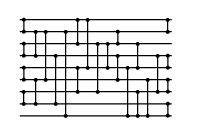
\includegraphics[scale=0.75]{\CURPATH/network9.png}
\caption{Smallest possible}
\end{figure}

This is combinational circuit, each connection is a comparator+swapper, it swaps if one of input values is bigger and passes output to the next level.

I copypasted it from \href{https://arxiv.org/pdf/1405.5754.pdf}{the article}:
Michael Codish, Lu ́ıs Cruz-Filipe, Michael Frank, and Peter Schneider-Kamp --
``Twenty-Five Comparators is Optimal when Sorting Nine Inputs (and Twenty-Nine for Ten)''.

Another article about it: \href{http://larc.unt.edu/ian/pubs/9-input.pdf}{Ian Parberry -- A Computer Assisted Optimal Depth Lower Bound for Nine-Input Sorting Networks}.

I don't know (yet) how they proved it, but it's interesting, that it's extremely easy to prove its correctness using Z3 SMT solver.
We just construct network out of comparators/swappers and asking Z3 to find counterexample, for which the output of the network will not be sorted.
And it can't, meaning, output's state is always sorted, no matter what values are plugged into inputs.

\lstinputlisting[style=custompy]{\CURPATH/test9.py}

( The full source code: \url{https://github.com/DennisYurichev/SAT_SMT_by_example/blob/master/proofs/sorting_network/test9.py}. )

There is also smaller 4-channel network I copypasted from Wikipedia:

\begin{lstlisting}
...

l=line(l, " + +")
l=line(l, "+ + ")
l=line(l, "++++")
l=line(l, " ++ ")

...
\end{lstlisting}

( The full source code: \url{https://github.com/DennisYurichev/SAT_SMT_by_example/blob/master/proofs/sorting_network/test4.py}. )

It also proved to be correct, but it's interesting, what Z3Py expression we've got at each of 4 outputs:

\begin{lstlisting}
If(If(a < c, a, c) < If(b < d, b, d),
   If(a < c, a, c),
   If(b < d, b, d))

If(If(If(a < c, a, c) > If(b < d, b, d),
      If(a < c, a, c),
      If(b < d, b, d)) <
   If(If(a > c, a, c) < If(b > d, b, d),
      If(a > c, a, c),
      If(b > d, b, d)),
   If(If(a < c, a, c) > If(b < d, b, d),
      If(a < c, a, c),
      If(b < d, b, d)),
   If(If(a > c, a, c) < If(b > d, b, d),
      If(a > c, a, c),
      If(b > d, b, d)))

If(If(If(a < c, a, c) > If(b < d, b, d),
      If(a < c, a, c),
      If(b < d, b, d)) >
   If(If(a > c, a, c) < If(b > d, b, d),
      If(a > c, a, c),
      If(b > d, b, d)),
   If(If(a < c, a, c) > If(b < d, b, d),
      If(a < c, a, c),
      If(b < d, b, d)),
   If(If(a > c, a, c) < If(b > d, b, d),
      If(a > c, a, c),
      If(b > d, b, d)))

If(If(a > c, a, c) > If(b > d, b, d),
   If(a > c, a, c),
   If(b > d, b, d))
\end{lstlisting}

The first and the last are shorter than the 2nd and the 3rd, they are just
$min(min(min(a,b),c),d)$ and 
$max(max(max(a,b),c),d)$.


\section{\ac{ITE} example}

From Daniel Kroening and Ofer Strichman - "Decision Procedures, An Algorithmic Point of View", 2ed:

\begin{lstlisting}

Problem 2.3 (modeling: program equivalence). Show that the two if-then-else expressions below are equivalent:

!(a || b) ? h : !(a == b) ? f : g

!(!a || !b) ? g : (!a && !b) ? h : f

You can assume that the variables have only one bit.

\end{lstlisting}

\lstinputlisting[style=customsmt]{proofs/ITE_equiv.smt}


\subsection{Branchless abs()}

Prove that branchless abs() function from the Henry Warren 2ed, "2-4 Absolute Value Function" is correct:

\lstinputlisting[style=customsmt]{proofs/abs.smt}


\subsection{Proving branchless min/max functions are correct}

... from \url{https://graphics.stanford.edu/~seander/bithacks.html#IntegerMinOrMax}.

Which are, $min(x,y) = y \oplus ((x \oplus y) \wedge (-(x < y)))$

And $max(x,y) = x \oplus ((x \oplus y) \wedge (-(x < y)))$

\lstinputlisting[label=Unsigned version,style=customsmt]{proofs/minmax.smt}

\lstinputlisting[label=Signed version,style=customsmt]{proofs/minmax_signed.smt}


\subsection{Proving ``Determine if a word has a zero byte'' bit twiddling hack}

... which is:

\begin{lstlisting}
#define haszero(v) (((v) - 0x01010101UL) & ~(v) & 0x80808080UL)
\end{lstlisting}

( \url{https://graphics.stanford.edu/~seander/bithacks.html#ZeroInWord} )

The expression returns zero if there are no zero bytes in 32-bit word, or non-zero, if at least one is present.
Here we prove that it's correct for all possible 32-bit words.

\lstinputlisting[style=customsmt]{proofs/nozerobytes.smt}


\subsection{Arithmetical shift bit twiddling hack}

Prove that \verb|((x+0x80000000) >>u n) - (0x80000000 >>u n)| 
works like arithmetical shift (\verb|bvashr| function in SMT-LIB or \verb|SAR| x86 instruction).

See: Henry Warren 2ed: "2-7 Shift Right Signed from Unsigned".

Also, check if I implemented signed shift right correctly in MK85:
\url{https://github.com/DennisYurichev/MK85/blob/834305a9851ec7976946247d42bb13d052aba005/MK85.cc#L1195}.

In other words, we prove equivalence of the expression above and my implementation.

\lstinputlisting{proofs/bvashr.smt}




\EN{\section{Regular expressions}

\section{KLEE}

I've always wanted to generate possible strings for given regular expression.
This is not so hard if to dive into regular expression matcher theory and details, but can we force RE matcher to do this?

I took lightest RE engine I've found: \url{https://github.com/cesanta/slre}, and wrote this:

% FIXME:
\begin{lstlisting}
int main(void)
{
	char s[6];
	klee_make_symbolic(s, sizeof s, "s");
	s[5]=0;
	if (slre_match("^\\d[a-c]+(x|y|z)", s, 5, NULL, 0, 0)==5)
		klee_assert(0);
}
\end{lstlisting}

So I wanted a string consisting of digit, ``a'' or ``b'' or ``c'' (at least one character) and ``x'' or ``y'' or ``z'' (one character).
The whole string must have size of 5 characters.

% FIXME:
\begin{lstlisting}
% klee --libc=uclibc slre.bc
...
KLEE: ERROR: /home/klee/slre.c:445: failed external call: klee_assert
KLEE: NOTE: now ignoring this error at this location
...

% ls klee-last | grep err
test000014.external.err

% ktest-tool --write-ints klee-last/test000014.ktest
ktest file : 'klee-last/test000014.ktest'
args       : ['slre.bc']
num objects: 1
object    0: name: b's'
object    0: size: 6
object    0: data: b'5aaax\xff'
\end{lstlisting}

This is indeed correct string. ``\textbackslash{}xff'' is at the place where terminal zero byte should be, but RE engine we use ignores the last zero byte, because it has buffer lenght as a passed parameter.
Hence, KLEE doesn't \textit{reconstruct} final byte.

Can we get more?
Now we add additional constraint:

\begin{lstlisting}
int main(void)
{
	char s[6];
	klee_make_symbolic(s, sizeof s, "s");
	s[5]=0;
	if (slre_match("^\\d[a-c]+(x|y|z)", s, 5, NULL, 0, 0)==5 &&
			strcmp(s, "5aaax")!=0)
		klee_assert(0);
}
\end{lstlisting}

% FIXME:
\begin{lstlisting}
% ktest-tool --write-ints klee-last/test000014.ktest
ktest file : 'klee-last/test000014.ktest'
args       : ['slre.bc']
num objects: 1
object    0: name: b's'
object    0: size: 6
object    0: data: b'7aaax\xff'
\end{lstlisting}

Let's say, out of whim, we don't like ``a'' at the 2nd position (starting at 0th):

% FIXME:
\begin{lstlisting}
int main(void)
{
	char s[6];
	klee_make_symbolic(s, sizeof s, "s");
	s[5]=0;
	if (slre_match("^\\d[a-c]+(x|y|z)", s, 5, NULL, 0, 0)==5 &&
			strcmp(s, "5aaax")!=0 &&
			s[2]!='a')
		klee_assert(0);
}
\end{lstlisting}

KLEE found a way to satisfy our new constraint:

% FIXME:
\begin{lstlisting}
% ktest-tool --write-ints klee-last/test000014.ktest
ktest file : 'klee-last/test000014.ktest'
args       : ['slre.bc']
num objects: 1
object    0: name: b's'
object    0: size: 6
object    0: data: b'7abax\xff'
\end{lstlisting}

Let's also define constraint KLEE cannot satisfy:

\begin{lstlisting}
int main(void)
{
	char s[6];
	klee_make_symbolic(s, sizeof s, "s");
	s[5]=0;
	if (slre_match("^\\d[a-c]+(x|y|z)", s, 5, NULL, 0, 0)==5 &&
			strcmp(s, "5aaax")!=0 &&
			s[2]!='a' &&
			s[2]!='b' &&
			s[2]!='c')
		klee_assert(0);
}
\end{lstlisting}

It cannot indeed, and KLEE finished without reporting about \TT{klee\_assert()} triggering.


\subsection{Enumerating all possible inputs for a specific regular expression}

\renewcommand{\CURPATH}{regexp/SMT}

Regular expression if first converted to \ac{FSM} before matching.
Hence, many \ac{RE} libraries has two functions: ``compile'' and ``execute''
(when you match many strings against single \ac{RE}, no need to recompile it to \ac{FSM} each time).

And I've found this website, which can visualize \ac{FSM} for a regular expression.
\url{http://hokein.github.io/Automata.js/}.
This is fun!

This \ac{FSM} (\ac{DFA}) is for the expression \TT{(dark|light)?(red|blue|green)(ish)?}

\begin{figure}[H]
\centering
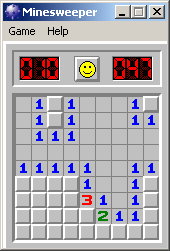
\includegraphics[scale=0.6]{\CURPATH/1.png}
\caption{}
\end{figure}

% FSM.png
Another version: URL.

Accepting states are in double circles, these are the states where matching process stops.

How can we generate an input string which regular expression would match?
In other words, which inputs \ac{FSM} would accept?
This task is surprisingly simple for SMT-solver.

We just define a transition function.
For each pair (state, input) it defines new state.

\ac{FSM} has been visualized by the website mentioned above, and I used this information to write ``transition()'' function.

Then we chain transition functions... then we try a chain for all lengths in range of 2..14.

\lstinputlisting{\CURPATH/re_MK85.py}

Results:

\lstinputlisting{\CURPATH/res.txt}

As simple as this.

The source code for Z3Py: \url{...re_Z3.py}.

% TODO \gls
It can be said, what we did is enumeration of all paths between two vertices of a digraph (representing \ac{FSM}).

Also, the ``transition()'' function itself can act as a RE matcher, with no relevance to SMT solver(s).
Just feed input characters to it and track state.
Whenever you hit one of accepting states, return ``match'', whenever you hit \TT{INVALID\_STATE}, return ``no match''.



}
\RU{\section{Регулярные выражения}

\subsection{KLEE}

Я всегда хотел как-нибудь сгенерировать возможные строки для определенного регулярного выражения.
Это не очень трудно, если окунуться в теорию стояющую за матчером регулярных выражений, но можно ли заставить
этот матчер сделать это?

Я нашел самый легковесный RE-движок здесь: \url{https://github.com/cesanta/slre}, и написал вот это:

\begin{lstlisting}
int main(void)
{
	char s[6];
	klee_make_symbolic(s, sizeof s, "s");
	s[5]=0;
	if (slre_match("^\\d[a-c]+(x|y|z)", s, 5, NULL, 0, 0)==5)
		klee_assert(0);
}
\end{lstlisting}

Так что я хотел строку состоящую из цифры, буквы ``a'' или ``b'' или ``c'' (как минимум один символ) и ``x'' или ``y'' или ``z'' (oдин символ).
Вся строка должна иметь размер в 5 символов.

\begin{lstlisting}
% klee --libc=uclibc slre.bc
...
KLEE: ERROR: /home/klee/slre.c:445: failed external call: klee_assert
KLEE: NOTE: now ignoring this error at this location
...

% ls klee-last | grep err
test000014.external.err

% ktest-tool --write-ints klee-last/test000014.ktest
ktest file : 'klee-last/test000014.ktest'
args       : ['slre.bc']
num objects: 1
object    0: name: b's'
object    0: size: 6
object    0: data: b'5aaax\xff'
\end{lstlisting}

Это действительно корректная строка, а на месте терминирующего нулевого байта находится ``\textbackslash{}xff'',
но RE-движок, который мы используем, игнорирует последний нулевой байт, потому ему передается длина буфера в отдельном параметре.
Следовательно, KLEE не \textit{реконструирует} последний байт.

Можем ли получить еще?
Добавляем дополнительный констрайнт:

\begin{lstlisting}
int main(void)
{
	char s[6];
	klee_make_symbolic(s, sizeof s, "s");
	s[5]=0;
	if (slre_match("^\\d[a-c]+(x|y|z)", s, 5, NULL, 0, 0)==5 &&
			strcmp(s, "5aaax")!=0)
		klee_assert(0);
}
\end{lstlisting}

\begin{lstlisting}
% ktest-tool --write-ints klee-last/test000014.ktest
ktest file : 'klee-last/test000014.ktest'
args       : ['slre.bc']
num objects: 1
object    0: name: b's'
object    0: size: 6
object    0: data: b'7aaax\xff'
\end{lstlisting}

Скажем так, просто из прихоти, нам не нравится буква ``a'' на второй позиции (если считать начиная с нулевой):

\begin{lstlisting}
int main(void)
{
	char s[6];
	klee_make_symbolic(s, sizeof s, "s");
	s[5]=0;
	if (slre_match("^\\d[a-c]+(x|y|z)", s, 5, NULL, 0, 0)==5 &&
			strcmp(s, "5aaax")!=0 &&
			s[2]!='a')
		klee_assert(0);
}
\end{lstlisting}

KLEE нашел способ удовлетворить этот новый констрайнт:

\begin{lstlisting}
% ktest-tool --write-ints klee-last/test000014.ktest
ktest file : 'klee-last/test000014.ktest'
args       : ['slre.bc']
num objects: 1
object    0: name: b's'
object    0: size: 6
object    0: data: b'7abax\xff'
\end{lstlisting}

Попробуем также определить констрайнт, который KLEE не сможет удовлетворить:

\begin{lstlisting}
int main(void)
{
	char s[6];
	klee_make_symbolic(s, sizeof s, "s");
	s[5]=0;
	if (slre_match("^\\d[a-c]+(x|y|z)", s, 5, NULL, 0, 0)==5 &&
			strcmp(s, "5aaax")!=0 &&
			s[2]!='a' &&
			s[2]!='b' &&
			s[2]!='c')
		klee_assert(0);
}
\end{lstlisting}

Действительно не может, и KLEE заканчивает работу без сообщения о входе в \TT{klee\_assert()}.


%\section{Развлекательная математика и головоломки}

\input{puzzles/sudoku/main_RU}
\input{puzzles/zebra/main_RU}
\input{puzzles/pipe/main_RU}
\input{puzzles/rubik2/failed_SMT/main_RU}
\input{puzzles/rubik2/SAT/main_RU}
\input{puzzles/rubik3/one_face_SMT/main_RU}
%\input{puzzles/numberlink/main_RU}
%\input{puzzles/two_parks_RU}
\input{puzzles/alphametics/main_RU}
%\input{puzzles/2015_AIME_II_Problems_12_RU}
%\input{puzzles/fred/main_RU}
%\input{puzzles/MC/main_RU}
%\input{puzzles/coin_flip/main_RU}
%\input{puzzles/Mock_AIME_2_2006-2007_Problem_8_RU}
%\input{puzzles/2012_AIME_I_Problems_1_RU}
%\input{puzzles/keypad_RU}



}


\section{Gray code}

\subsection{Balanced Gray code and Z3 SMT solver}
\label{Gray_Z3}

\renewcommand{\CURPATH}{gray_code/SMT}

Suppose, you are making a rotary encoder.
This is a device that can signal its angle in some form, like:

\begin{figure}[H]
\centering
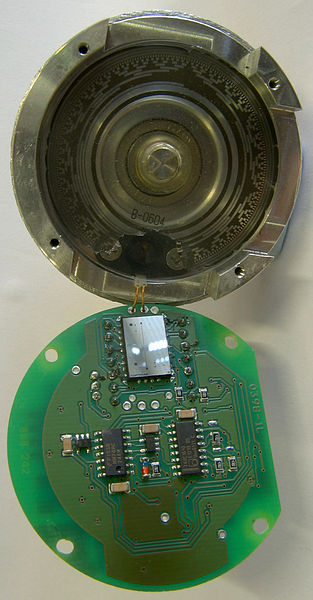
\includegraphics[scale=1]{\CURPATH/313px-Gray_code_rotary_encoder_13-track_opened.jpg}
\caption{Rotary encoder}
\end{figure}

( The image has been taken from Wikipedia: \url{https://en.wikipedia.org/wiki/Gray_code} )

Click on \href{https://github.com/DennisYurichev/SAT_SMT_by_example/blob/master/gray_code/SMT/Gray_code_rotary_encoder_13-track_opened.jpg}{bigger image}.

This is a rotary (shaft) encoder: \url{https://en.wikipedia.org/wiki/Rotary_encoder}.

\begin{figure}[H]
\centering
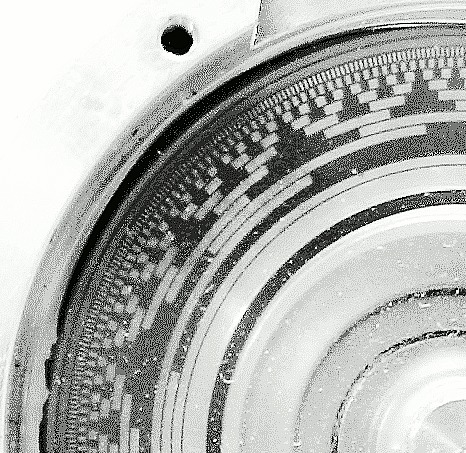
\includegraphics[scale=0.8]{\CURPATH/Rotary_Encoder_track_detail_scaled_crop.jpg}
\caption{Cropped and photoshopped version}
\end{figure}

( Source: \url{http://homepages.dordt.edu/~ddeboer//S10/304/c_at_d/304S10_RC_TRK.HTM} )

Click on
\href{https://github.com/DennisYurichev/SAT_SMT_by_example/blob/master/gray_code/SMT/Rotary_Encoder_track_detail.jpg}{bigger one}.

There are pins and tracks on rotating wheel.
How would you do this?
Easiest way is to use binary code.
But it has a problem: when a wheel is rotating, in a moment of transition from one state to another, several bits may be changed, hence, undesirable state may be present for a short period of time.
This is bad.
To deal with it, Gray code was invented: only 1 bit is changed during rotation.
Like:

\begin{lstlisting}
Decimal Binary  Gray
0 	0000 	0000
1 	0001 	0001
2 	0010 	0011
3 	0011 	0010
4 	0100 	0110
5 	0101 	0111
6 	0110 	0101
7 	0111 	0100
8 	1000 	1100
9 	1001 	1101
10 	1010 	1111
11 	1011 	1110
12 	1100 	1010
13 	1101 	1011
14 	1110 	1001
15 	1111 	1000
\end{lstlisting}

Now the second problem. Look at the picture again. It has a lot of bit changes on the outer circles.
And this is electromechanical device.
Surely, you may want to make tracks as long as possible, to reduce wearing of both tracks and pins.
This is a first problem.
The second: wearing should be even across all tracks (this is balanced Gray code).

This is also called:
"They are listed in Gray code or minimum change order, where each subset differs in exactly one element from its neighbors."
( Sriram V. Pemmaraju and Steven Skiena -- Computational Discrete Mathematics: Combinatorics and Graph Theory in Mathematica )

How we can find a table for all states using Z3:

\lstinputlisting[style=custompy]{\CURPATH/gray.py}

( The source code: \url{https://github.com/DennisYurichev/SAT_SMT_by_example/blob/master/gray_code/SMT/gray.py} )

For 4 bits, 4 changes is enough:

\lstinputlisting{\CURPATH/4.txt}

8 changes for 5 bits: \url{https://github.com/DennisYurichev/SAT_SMT_by_example/blob/master/gray_code/SMT/5.txt}.
12 for 6 bits (or maybe even less): 
\url{https://github.com/DennisYurichev/SAT_SMT_by_example/blob/master/gray_code/SMT/6.txt}.

\subsubsection{Duke Nukem 3D from 1990s}

\begin{figure}[H]
\centering
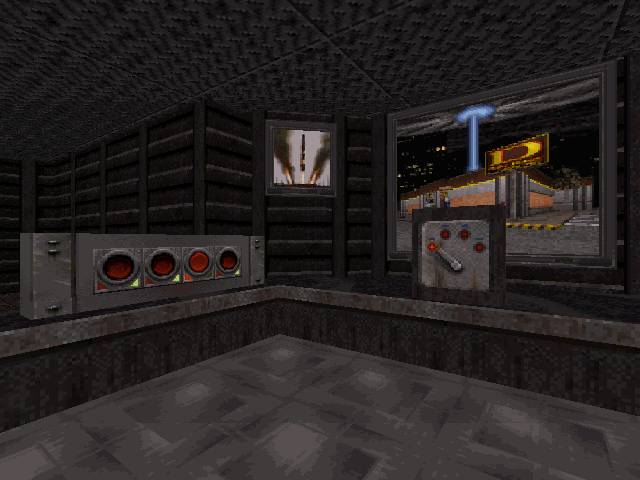
\includegraphics[scale=3]{\CURPATH/duke.png}
\caption{Duke Nukem 3D}
\end{figure}

Another application of Gray code:

\begin{lstlisting}
with.inspiring@flair.and.erudition (Mike Naylor) wrote:

>In Duke Nukem, you often come upon panels that have four buttons in a row,
>all in their "off" position. Each time you "push" a button, it toggles from
>one state to the other. The object is to find the unique combination that
>unlocks something in the game.

>My question is: What is the most efficient order in which to push the
>buttons so that every combination is tested with no wasted effort?

A Gray Code. :-)

(Oh, you wanted to know what one would be?  How about:
0000
0001
0011
0010
0110
0111
0101
0100
1100
1101
1111
1110
1010
1000
1001
1011

Or, if you prefer, with buttons A,B,C,D: D,C,D,B,D,C,D,A,D,C,D,B,C,D,C
It isn't the "canonical" Gray code (or if it is, it is by Divine
Providence), but it works.

Douglas Limmer -- lim...@math.orst.edu
"No wonder these mathematical wizards were nuts - went off the beam -
he'd be pure squirrel-food if he had half that stuff in _his_ skull!"
E. E. "Doc" Smith, _Second Stage Lensmen_
\end{lstlisting}

( \url{https://groups.google.com/forum/#!topic/rec.puzzles/Dh2H-pGJcbI} )

Obviously, using our solution, you can minimize all movements in this ancient videogame, for 4 switches, that would be 4*4=16 switches.
With our solution (balanced Gray code), wearing would be even across all 4 switches.

\subsubsection{Towers of Hanoi}

"The standard n-bit Gray code gives a solution to the Towers of Hanoi problem with n levels.
The position of the bit that changes tells us which level of the tower we must move."
( \url{http://www.maths.liv.ac.uk/~mathsclub/talks/20160130/talk1/joel_summary.pdf} ).


\subsection{Gray code in MaxSAT}
\label{Gray_MaxSAT}

\renewcommand{\CURPATH}{gray_code/MaxSAT}

This is remake of gray code generator for Z3 (\ref{Gray_Z3}).

Here is also \textit{ch[]} table, but we add soft clauses for it here.
The goal is to make as many \textit{False}'s in \textit{ch[]} table, as possible.

\lstinputlisting{\CURPATH/gray_SAT.py}

So it does, for 5-bit Gray code:

\lstinputlisting{\CURPATH/5.txt}




\chapter{Recreational mathematics and puzzles}

\subsection{Sudoku}

Sudoku puzzle is a 9*9 grid with some cells filled with values, some are empty:

% copypasted from http://www.texample.net/tikz/examples/sudoku/
\newcounter{row}
\newcounter{col}

\newcommand\setrow[9]{
  \setcounter{col}{1}
  \foreach \n in {#1, #2, #3, #4, #5, #6, #7, #8, #9} {
    \edef\x{\value{col} - 0.5}
    \edef\y{9.5 - \value{row}}
    \node[anchor=center] at (\x, \y) {\n};
    \stepcounter{col}
  }
  \stepcounter{row}
}

\begin{center}
\begin{tikzpicture}[scale=.7]
  \begin{scope}
    \draw (0, 0) grid (9, 9);
    \draw[very thick, scale=3] (0, 0) grid (3, 3);

    \setcounter{row}{1}
    \setrow { }{ }{5}  {3}{ }{ }  { }{ }{ }
    \setrow {8}{ }{ }  { }{ }{ }  { }{2}{ }
    \setrow { }{7}{ }  { }{1}{ }  {5}{ }{ }

    \setrow {4}{ }{ }  { }{ }{5}  {3}{ }{ }
    \setrow { }{1}{ }  { }{7}{ }  { }{ }{6}
    \setrow { }{ }{3}  {2}{ }{ }  { }{8}{ }

    \setrow { }{6}{ }  {5}{ }{ }  { }{ }{9}
    \setrow { }{ }{4}  { }{ }{ }  { }{3}{ }
    \setrow { }{ }{ }  { }{ }{9}  {7}{ }{ }

    \node[anchor=center] at (4.5, -0.5) {Unsolved Sudoku};
  \end{scope}
\end{tikzpicture}
\end{center}

Numbers of each row must be unique, i.e., it must contain all 9 numbers in range of 1..9 without repetition.
Same story for each column and also for each 3*3 square.

This puzzle is good candidate to try \ac{SMT} solver on, because it's essentially an unsolved system of equations.

\subsubsection{Simple sudoku in SMT}
\label{sudoku_SMT}

\paragraph{The first idea}

The only thing we must decide is that how to determine in one expression, if the input 9 variables has all 9 unique numbers?
They are not ordered or sorted, after all.

From the school-level arithmetics, we can devise this idea:

\begin{equation}
\underbrace{10^{i_1} + 10^{i_2} + \cdots + 10^{i_9}}_9 = 1111111110
\end{equation}

Take each input variable, calculate $10^i$ and sum them all.
If all input values are unique, each will be settled at its own place.
Even more than that: there will be no holes, i.e., no skipped values.
So, in case of Sudoku, 1111111110 number will be final result, indicating that all 9 input values are unique, in range of 1..9.

Exponentiation is heavy operation, can we use binary operations? Yes, just replace 10 with 2:

\begin{equation}
\underbrace{2^{i_1} + 2^{i_2} + \cdots + 2^{i_9}}_9 = 1111111110_2
\end{equation}

The effect is just the same, but the final value is in base 2 instead of 10.

Now a working example:

\lstinputlisting[style=custompy]{puzzles/sudoku/1/sudoku_plus_Z3.py}
( \url{https://github.com/DennisYurichev/SAT_SMT_by_example/blob/master/puzzles/sudoku/1/sudoku_plus_Z3.py} )

\begin{lstlisting}
% time python sudoku_plus_Z3.py
1 4 5 3 2 7 6 9 8
8 3 9 6 5 4 1 2 7
6 7 2 9 1 8 5 4 3
4 9 6 1 8 5 3 7 2
2 1 8 4 7 3 9 5 6
7 5 3 2 9 6 4 8 1
3 6 7 5 4 2 8 1 9
9 8 4 7 6 1 2 3 5
5 2 1 8 3 9 7 6 4

real    0m11.717s
user    0m10.896s
sys     0m0.068s
\end{lstlisting}

Even more, we can replace summing operation to logical OR:

\begin{equation}
\underbrace{2^{i_1} \vee 2^{i_2} \vee \cdots \vee 2^{i_9}}_9 = 1111111110_2
\end{equation}

% FIXME: только часть исходника
\lstinputlisting[style=custompy]{puzzles/sudoku/1/sudoku_or_Z3.py}
( \url{https://github.com/DennisYurichev/SAT_SMT_by_example/blob/master/puzzles/sudoku/1/sudoku_or_Z3.py} )

Now it works much faster. Z3 handles OR operation over bit vectors better than addition?

\begin{lstlisting}
% time python sudoku_or_Z3.py
1 4 5 3 2 7 6 9 8
8 3 9 6 5 4 1 2 7
6 7 2 9 1 8 5 4 3
4 9 6 1 8 5 3 7 2
2 1 8 4 7 3 9 5 6
7 5 3 2 9 6 4 8 1
3 6 7 5 4 2 8 1 9
9 8 4 7 6 1 2 3 5
5 2 1 8 3 9 7 6 4

real    0m1.429s
user    0m1.393s
sys     0m0.036s
\end{lstlisting}

The puzzle I used as example is dubbed as one of the hardest known
\footnote{\url{http://www.mirror.co.uk/news/weird-news/worlds-hardest-sudoku-can-you-242294}} (well, for humans).
It took $\approx 1.4$ seconds on my Intel Core i3-3110M 2.4GHz notebook to solve it.

\paragraph{The second idea}

My first approach is far from effective, I did what first came to my mind and worked.
Another approach is to use \TT{distinct} command from SMT-LIB, which tells Z3 that some variables must be distinct (or unique).
This command is also available in Z3 Python interface.

I've rewritten my first Sudoku solver, now it operates over \textit{Int} \textit{sort}, it has \TT{distinct} commands instead of bit operations,
and now also other constaint added: each cell value must be in 1..9 range, because, otherwise, Z3 will offer (although correct) solution with too big
and/or negative numbers.

% FIXME: только часть исходника
\lstinputlisting[style=custompy]{puzzles/sudoku/1/sudoku2_Z3.py}
( \url{https://github.com/DennisYurichev/SAT_SMT_by_example/blob/master/puzzles/sudoku/1/sudoku2_Z3.py} )

\begin{lstlisting}
% time python sudoku2_Z3.py
1 4 5 3 2 7 6 9 8
8 3 9 6 5 4 1 2 7
6 7 2 9 1 8 5 4 3
4 9 6 1 8 5 3 7 2
2 1 8 4 7 3 9 5 6
7 5 3 2 9 6 4 8 1
3 6 7 5 4 2 8 1 9
9 8 4 7 6 1 2 3 5
5 2 1 8 3 9 7 6 4

real    0m0.382s
user    0m0.346s
sys     0m0.036s
\end{lstlisting}

That's much faster.

\paragraph{Conclusion}

\ac{SMT}-solvers are so helpful, is that our Sudoku solver has nothing else, we have just defined relationships between variables (cells).

\paragraph{Homework}

As it seems, true Sudoku puzzle is the one which has only one solution.
The piece of code I've included here shows only the first one.
Using the method described earlier (\ref{SMTEnumerate}, also called ``model counting''), 
try to find more solutions, or prove that the solution you have just found is the only one possible.

\paragraph{Further reading}

\url{http://www.norvig.com/sudoku.html}

\paragraph{Sudoku as a \ac{SAT} problem}

It's also possible to represend Sudoku puzzle as a huge \ac{CNF} equation and use \ac{SAT}-solver to find solution, but it's just trickier.

Some articles about it:
\textit{Building a Sudoku Solver with SAT}\footnote{\url{https://dspace.mit.edu/bitstream/handle/1721.1/106923/6-005-fall-2011/contents/assignments/MIT6_005F11_ps4.pdf}},
Tjark Weber, \textit{A SAT-based Sudoku Solver}\footnote{\url{https://www.lri.fr/~conchon/mpri/weber.pdf}},
Ines Lynce, Joel Ouaknine, \textit{Sudoku as a SAT Problem}\footnote{\url{http://sat.inesc-id.pt/~ines/publications/aimath06.pdf}},
Gihwon Kwon, Himanshu Jain, \textit{Optimized CNF Encoding for Sudoku Puzzles}\footnote{\url{http://www.cs.cmu.edu/~hjain/papers/sudoku-as-SAT.pdf}}.

\ac{SMT}-solver can also use \ac{SAT}-solver in its core, so it does all mundane translating work.
As a ``compiler'', it may not do this in the most efficient way, though.


\subsubsection{Greater Than Sudoku}

I've found this on \url{http://www.killersudokuonline.com}:

\begin{figure}[H]
\centering
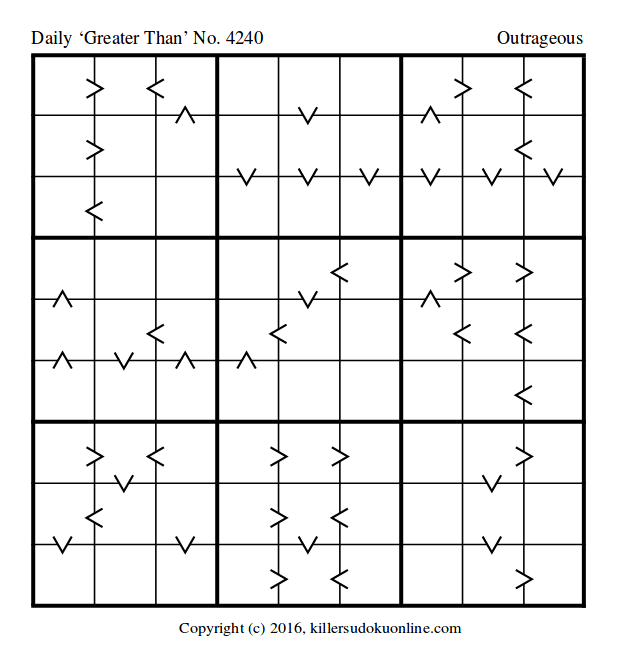
\includegraphics[scale=0.6]{puzzles/sudoku/GT/puzzle.png}
\caption{}
\end{figure}

% TODO \ref
It can be solved easily with Z3. I've took the same piece of code I used for the usual Sudoku: ().
% ( _HTML_LINK_AS_IS(`https://github.com/DennisYurichev/SAT_SMT_article/blob/master/SMT/sudoku2.py'), 

... and added this:</p>

\begin{lstlisting}
...

"""
Subsquares:

------------------------------
         |          |         
 1,1     | 1,2      | 1,3     
         |          |         
------------------------------
         |          |         
 2,1     | 2,2      | 2,3     
         |          |         
------------------------------
         |          |         
 3,1     | 3,2      | 3,3     
         |          |         
------------------------------
"""

# from http://www.killersudokuonline.com/puzzles/2017/puzzle-GD4hzi164344.pdf

# subsquare 1,1:
s.add(cells[0][0]>cells[0][1])
s.add(cells[1][0]>cells[1][1])
s.add(cells[2][0]<cells[2][1])

s.add(cells[0][1]<cells[0][2])
s.add(cells[0][2]<cells[1][2])

# subsquare 1,2:
s.add(cells[0][4]>cells[1][4])
s.add(cells[1][3]>cells[2][3])
s.add(cells[1][4]>cells[2][4])
s.add(cells[1][5]>cells[2][5])

# subsquare 1,3:
s.add(cells[0][6]>cells[0][7])
s.add(cells[0][7]<cells[0][8])
s.add(cells[0][6]<cells[1][6])
s.add(cells[1][7]<cells[1][8])
s.add(cells[1][6]>cells[2][6])
s.add(cells[1][7]>cells[2][7])
s.add(cells[1][8]>cells[2][8])

# subsquare 2,1:
s.add(cells[3][0]<cells[4][0])
s.add(cells[4][0]<cells[5][0])
s.add(cells[4][1]<cells[4][2])
s.add(cells[4][0]<cells[5][0])
s.add(cells[4][1]>cells[5][1])
s.add(cells[4][2]<cells[5][2])

# subsquare 2,2:
s.add(cells[3][4]>cells[4][4])
s.add(cells[3][4]<cells[3][5])
s.add(cells[4][3]<cells[4][4])
s.add(cells[4][3]<cells[5][3])

# subsquare 2,3:
s.add(cells[3][6]>cells[3][7])
s.add(cells[3][7]>cells[3][8])
s.add(cells[3][6]>cells[4][6])
s.add(cells[4][6]<cells[4][7])
s.add(cells[4][7]<cells[4][8])
s.add(cells[5][7]<cells[5][8])

# subsquare 3,1:
s.add(cells[6][0]>cells[6][1])
s.add(cells[6][1]<cells[6][2])
s.add(cells[6][1]>cells[7][1])
s.add(cells[7][0]<cells[7][1])
s.add(cells[7][0]>cells[8][0])
s.add(cells[7][2]>cells[8][2])

# subsquare 3,2:
s.add(cells[6][3]>cells[6][4])
s.add(cells[6][4]>cells[6][5])
s.add(cells[7][3]>cells[7][4])
s.add(cells[7][4]<cells[7][5])
s.add(cells[8][3]>cells[8][4])
s.add(cells[8][4]<cells[8][5])
s.add(cells[7][4]>cells[8][4])

# subsquare 3,3:
s.add(cells[6][7]>cells[6][8])
s.add(cells[6][7]>cells[7][7])
s.add(cells[7][7]>cells[8][7])
s.add(cells[8][7]>cells[8][8])

...
\end{lstlisting}

( The full file: \url{https://github.com/DennisYurichev/yurichev.com/.../sudoku_GT.py} )

The puzzle marked as ``Outrageous'' (for humans?), however it took $\approx 30$ seconds
on my old Intel Xeon E3-1220 3.10GHz to solve it:

\begin{lstlisting}
7 3 4 6 9 2 5 1 8
2 1 5 8 3 7 9 4 6
6 8 9 5 1 4 7 2 3
1 7 3 2 8 9 6 5 4
5 4 6 1 7 3 2 8 9
9 2 8 4 5 6 1 3 7
8 6 7 3 2 1 4 9 5
4 5 2 9 6 8 3 7 1
3 9 1 7 4 5 8 6 2
\end{lstlisting}


\subsubsection{Solving Killer Sudoku}

I've found this on \url{https://krazydad.com/killersudoku/sfiles/KD_Killer_ST16_8_v52.pdf}:

\begin{figure}[H]
\centering
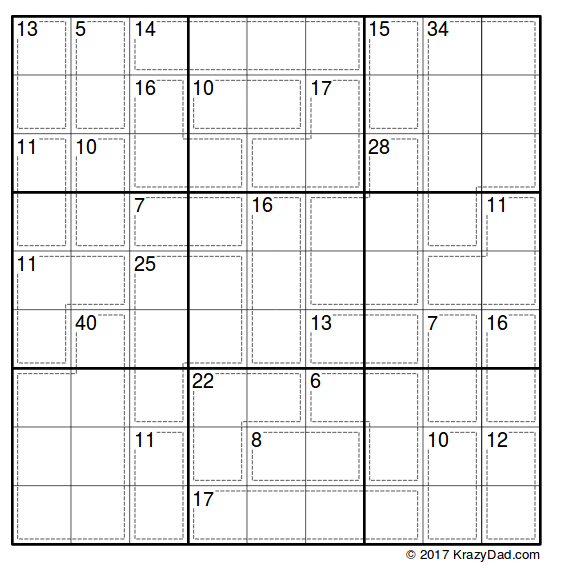
\includegraphics[scale=0.6]{puzzles/sudoku/killer/puzzle.png}
\caption{}
\end{figure}

There are ``cages'', each cage must have distinct digits,
and its sum must be equal to the number written there in a manner of crossword.
See also: \url{https://en.wikipedia.org/wiki/Killer_sudoku}.

This is also piece of cake for Z3.
% TODO \ref
I've took the same piece of code I used for usual Sudoku ( \url{...sudoku2.py} ).

\begin{lstlisting}
...

cage=[cells[0][0], cells[1][0]]
s.add(Distinct(*cage))
s.add(Sum(*cage)==13)

cage=[cells[0][1], cells[1][1]]
s.add(Distinct(*cage))
s.add(Sum(*cage)==5)

cage=[cells[0][2], cells[0][3], cells[0][4], cells[0][5]]
s.add(Distinct(*cage))
s.add(Sum(*cage)==14)

cage=[cells[0][6], cells[1][6]]
s.add(Distinct(*cage))
s.add(Sum(*cage)==15)

cage=[cells[0][7], cells[0][8], cells[1][7], cells[1][8], cells[2][7], cells[2][8], cells[3][7]]
s.add(Distinct(*cage))
s.add(Sum(*cage)==34)

cage=[cells[1][2], cells[2][2], cells[2][3]]
s.add(Distinct(*cage))
s.add(Sum(*cage)==16)

cage=[cells[1][3], cells[1][4]]
s.add(Distinct(*cage))
s.add(Sum(*cage)==10)

cage=[cells[1][5], cells[2][4], cells[2][5]]
s.add(Distinct(*cage))
s.add(Sum(*cage)==17)

cage=[cells[2][6], cells[3][5], cells[3][6], cells[4][5], cells[4][6]]
s.add(Distinct(*cage))
s.add(Sum(*cage)==28)

cage=[cells[3][2], cells[3][3]]
s.add(Distinct(*cage))
s.add(Sum(*cage)==7)

cage=[cells[3][4], cells[4][4], cells[5][4]]
s.add(Distinct(*cage))
s.add(Sum(*cage)==16)

cage=[cells[3][8], cells[4][7], cells[4][8]]
s.add(Distinct(*cage))
s.add(Sum(*cage)==11)

cage=[cells[4][0], cells[4][1], cells[5][0]]
s.add(Distinct(*cage))
s.add(Sum(*cage)==11)

cage=[cells[4][2], cells[4][3], cells[5][2], cells[5][3], cells[6][2]]
s.add(Distinct(*cage))
s.add(Sum(*cage)==25)

cage=[cells[5][1], cells[6][0], cells[6][1], cells[7][0], cells[7][1], cells[8][0], cells[8][1]]
s.add(Distinct(*cage))
s.add(Sum(*cage)==40)

cage=[cells[5][5], cells[5][6]]
s.add(Distinct(*cage))
s.add(Sum(*cage)==13)

cage=[cells[5][7], cells[6][7]]
s.add(Distinct(*cage))
s.add(Sum(*cage)==7)

cage=[cells[5][8], cells[6][8]]
s.add(Distinct(*cage))
s.add(Sum(*cage)==16)

cage=[cells[6][3], cells[6][4], cells[7][3]]
s.add(Distinct(*cage))
s.add(Sum(*cage)==22)

cage=[cells[6][5], cells[6][6], cells[7][6]]
s.add(Distinct(*cage))
s.add(Sum(*cage)==6)

cage=[cells[7][2], cells[8][2]]
s.add(Distinct(*cage))
s.add(Sum(*cage)==11)

cage=[cells[7][4], cells[7][5]]
s.add(Distinct(*cage))
s.add(Sum(*cage)==8)

cage=[cells[7][7], cells[8][7]]
s.add(Distinct(*cage))
s.add(Sum(*cage)==10)

cage=[cells[7][8], cells[8][8]]
s.add(Distinct(*cage))
s.add(Sum(*cage)==12)

cage=[cells[8][3], cells[8][4], cells[8][5], cells[8][6]]
s.add(Distinct(*cage))
s.add(Sum(*cage)==17)

...
\end{lstlisting}

( The full file: \url{...killer_sudoku.py} )

The puzzle marked as ``Super-Tough Killer Sudoku Puzzle'' (again, for humans?),
however it took $\approx 30$ seconds on my old Intel Xeon E3-1220 3.10GHz to solve it:

\begin{lstlisting}
5 3 4 7 1 2 8 9 6
8 2 1 4 6 9 7 5 3
9 6 7 8 3 5 4 2 1
2 4 6 1 9 7 3 8 5
7 1 9 3 5 8 6 4 2
3 8 5 6 2 4 9 1 7
4 7 2 5 8 3 1 6 9
6 5 8 9 7 1 2 3 4
1 9 3 2 4 6 5 7 8
\end{lstlisting}


\subsubsection{KLEE}

I've also rewritten Sudoku example (\ref{sudoku_SMT}) for KLEE:

\lstinputlisting[numbers=left]{puzzles/sudoku/KLEE/klee_sudoku_or1.c}

Let's run it:

\begin{lstlisting}
% clang -emit-llvm -c -g klee_sudoku_or1.c
...

\$ time klee klee_sudoku_or1.bc
KLEE: output directory is "/home/klee/klee-out-98"
KLEE: WARNING: undefined reference to function: klee_assert
KLEE: WARNING ONCE: calling external: klee_assert(0)
KLEE: ERROR: /home/klee/klee_sudoku_or1.c:93: failed external call: klee_assert
KLEE: NOTE: now ignoring this error at this location

KLEE: done: total instructions = 7512
KLEE: done: completed paths = 161
KLEE: done: generated tests = 161

real    3m44.111s
user    3m43.319s
sys     0m0.951s
\end{lstlisting}

Now this is really slower (on my Intel Core i3-3110M 2.4GHz notebook) in comparison to Z3Py solution (\ref{sudoku_SMT}).

But the answer is correct:

\begin{lstlisting}
% ls klee-last | grep err
test000161.external.err

% ktest-tool --write-ints klee-last/test000161.ktest
ktest file : 'klee-last/test000161.ktest'
args       : ['klee_sudoku_or1.bc']
num objects: 1
object    0: name: b'cells'
object    0: size: 81
object    0: data: b'\x01\x04\x05\x03\x02\x07\x06\t\x08\x08\x03\t\x06\x05\x04\x01\x02\x07\x06\x07\x02\t\x01\x08\x05\x04\x03\x04\t\x06\x01\x08\x05\x03\x07\x02\x02\x01\x08\x04\x07\x03\t\x05\x06\x07\x05\x03\x02\t\x06\x04\x08\x01\x03\x06\x07\x05\x04\x02\x08\x01\t\t\x08\x04\x07\x06\x01\x02\x03\x05\x05\x02\x01\x08\x03\t\x07\x06\x04'
\end{lstlisting}

Character \TT{\textbackslash{}t} has code of 9 in C/C++,
and KLEE prints byte array as a C/C++ string, so it shows some values in such way.
We can just keep in mind that there is 9 at the each place where we see \TT{\textbackslash{}t}.
The solution, while not properly formatted, correct indeed.

By the way, at lines 42 and 43 you may see how we tell to KLEE that all array elements must be within some limits.
If we comment these lines out, we've got this:

\begin{lstlisting}
% time klee klee_sudoku_or1.bc
KLEE: output directory is "/home/klee/klee-out-100"
KLEE: WARNING: undefined reference to function: klee_assert
KLEE: ERROR: /home/klee/klee_sudoku_or1.c:51: overshift error
KLEE: NOTE: now ignoring this error at this location
KLEE: ERROR: /home/klee/klee_sudoku_or1.c:51: overshift error
KLEE: NOTE: now ignoring this error at this location
KLEE: ERROR: /home/klee/klee_sudoku_or1.c:51: overshift error
KLEE: NOTE: now ignoring this error at this location
...
\end{lstlisting}

KLEE warns us that shift value at line 51 is too big.
Indeed, KLEE may try all byte values up to 255 (0xFF), which are pointless to use there,
and may be a symptom of error or bug, so KLEE warns about it. % FIXME chk spelling

Now let's use \TT{klee\_assume()} again:

\lstinputlisting{puzzles/sudoku/KLEE/klee_sudoku_or2.c}

\begin{lstlisting}
% time klee klee_sudoku_or2.bc
KLEE: output directory is "/home/klee/klee-out-99"
KLEE: WARNING: undefined reference to function: klee_assert
KLEE: WARNING ONCE: calling external: klee_assert(0)
KLEE: ERROR: /home/klee/klee_sudoku_or2.c:93: failed external call: klee_assert
KLEE: NOTE: now ignoring this error at this location

KLEE: done: total instructions = 7119
KLEE: done: completed paths = 1
KLEE: done: generated tests = 1

real    0m35.312s
user    0m34.945s
sys     0m0.318s
\end{lstlisting}

That works much faster: perhaps KLEE indeed handle this \textit{intrinsic} in a special way.
And, as we see, the only one path has been found (one we actually interesting in it) instead of 161.

It's still much slower than Z3Py solution, though.


\subsubsection{Sudoku in SAT}
\label{Sudoku_SAT}

One might think that we can encode each 1..9 number in binary form: 5 bits or variables would be enough.
But there is even simpler way: allocate 9 bits, where only one bit will be \textit{True}.
The number 1 can be encoded as [1, 0, 0, 0, 0, 0, 0, 0, 0], the number 3 as [0, 0, 1, 0, 0, 0, 0, 0, 0], etc.
Seems uneconomical? Yes, but other operations would be simpler.

First of all, we'll reuse important \TT{POPCNT1} function I've described earlier: \ref{POPCNTOne}.

The second important operation we need to invent is making 9 numbers unique.
If each number is encoded as 9-bits vector, 9 numbers can form a matrix, like:

\begin{lstlisting}
0 0 0 0 0 0 1 0 0 <- 1st number
0 0 0 0 0 1 0 0 0 <- 2nd number
0 1 0 0 0 0 0 0 0 <- ...
0 0 1 0 0 0 0 0 0 <- ...
0 0 0 0 0 0 0 0 1 <- ...
0 0 0 0 1 0 0 0 0 <- ...
0 0 0 0 0 0 0 1 0 <- ...
1 0 0 0 0 0 0 0 0 <- ...
0 0 0 1 0 0 0 0 0 <- 9th number
\end{lstlisting}

Now we will use a \TT{POPCNT1} function to make each row in the matrix to contain only one \textit{True} bit, that will
preserve consistency in encoding, since no vector can contain more than 1 \textit{True} bit, or no \textit{True} bits at all.
Then we will use a \TT{POPCNT1} function again to make all columns in the matrix to have only one single \textit{True} bit.
That will make all rows in matrix unique, in other words, all 9 encoded numbers will always be unique.

After applying \TT{POPCNT1} function 9+9=18 times we'll have 9 unique numbers in 1..9 range.

Using that operation we can make each row of Sudoku puzzle unique, each column unique and also each $3 \cdot 3=9$ box.

\lstinputlisting[style=custompy]{puzzles/sudoku/SAT/sudoku_SAT.py}
( \url{https://github.com/DennisYurichev/SAT_SMT_by_example/blob/master/puzzles/sudoku/SAT/sudoku_SAT.py} )

The \TT{make\_distinct\_bits\_in\_vector()} function preserves consistency of encoding.\\
The \TT{make\_distinct\_vectors()} function makes 9 numbers unique.\\
The \TT{cvt\_vector\_to\_number()} decodes vector to number.\\
The \TT{number\_to\_vector()} encodes number to vector.\\
The \TT{main()} function has all necessary calls to make rows/columns/$3\cdot 3$ boxes unique.

That works:

\begin{lstlisting}
% python sudoku_SAT.py
len(clauses)= 12195
1 4 5 3 2 7 6 9 8
8 3 9 6 5 4 1 2 7
6 7 2 9 1 8 5 4 3
4 9 6 1 8 5 3 7 2
2 1 8 4 7 3 9 5 6
7 5 3 2 9 6 4 8 1
3 6 7 5 4 2 8 1 9
9 8 4 7 6 1 2 3 5
5 2 1 8 3 9 7 6 4
\end{lstlisting}

Same solution as earlier: \ref{sudoku_SMT}.

Picosat tells this SAT instance has only one solution.
Indeed, as they say, true Sudoku puzzle can have only one solution.

\paragraph{Getting rid of one POPCNT1 function call}
\label{OR_in_POPCNT1}

To make 9 unique 1..9 numbers we can use \TT{POPCNT1} function to make each row in matrix be unique and
use \textit{OR} boolean operation for all columns.
That will have merely the same effect: all rows has to be unique to make each column to be evaluated
to \textit{True} if all variables in column are OR'ed.
(I will do this in the next example: \ref{Zebra_SAT}.)

That will make 3447 clauses instead of 12195, but somehow, SAT solvers works slower. No idea why.




\section{Zebra puzzle (\ac{AKA} Einstein puzzle)}

\subsection{SMT}
\label{zebra_SMT}

Zebra puzzle is a popular puzzle, defined as follows:

% FIXME remove paragraph at first line
\begin{framed}
\begin{quotation}
1.There are five houses.\\
2.The Englishman lives in the red house.\\
3.The Spaniard owns the dog.\\
4.Coffee is drunk in the green house.\\
5.The Ukrainian drinks tea.\\
6.The green house is immediately to the right of the ivory house.\\
7.The Old Gold smoker owns snails.\\
8.Kools are smoked in the yellow house.\\
9.Milk is drunk in the middle house.\\
10.The Norwegian lives in the first house.\\
11.The man who smokes Chesterfields lives in the house next to the man with the fox.\\
12.Kools are smoked in the house next to the house where the horse is kept.\\
13.The Lucky Strike smoker drinks orange juice.\\
14.The Japanese smokes Parliaments.\\
15.The Norwegian lives next to the blue house.\\
\\
Now, who drinks water? Who owns the zebra?\\
\\
In the interest of clarity, it must be added that each of the five houses is painted a different color, and their inhabitants are of different national extractions, own different pets, drink different beverages and smoke different brands of American cigarets [sic]. One other thing: in statement 6, right means your right.
\end{quotation}
\end{framed}
( \url{https://en.wikipedia.org/wiki/Zebra_Puzzle} ) \\
\\
It's a very good example of \ac{CSP}.

We would encode each entity as integer variable, representing number of house.

Then, to define that Englishman lives in red house, we will add this constraint: \TT{Englishman == Red}, meaning that number of a house where Englishmen resides and which is painted in red is the same.

To define that Norwegian lives next to the blue house, we don't realy know, if it is at left side of blue house or at right side, but we know that house numbers are different by just 1.
So we will define this constraint: \TT{Norwegian==Blue-1 OR Norwegian==Blue+1}.

We will also need to limit all house numbers, so they will be in range of 1..5.

We will also use \TT{Distinct} to show that all various entities of the same type are all has different house numbers.

\lstinputlisting[style=custompy]{puzzles/zebra/SMT/zebra.py}

When we run it, we got correct result:

\begin{lstlisting}
sat
[Snails = 3,
 Blue = 2,
 Ivory = 4,
 OrangeJuice = 4,
 Parliament = 5,
 Yellow = 1,
 Fox = 1,
 Zebra = 5,
 Horse = 2,
 Dog = 4,
 Tea = 2,
 Water = 1,
 Chesterfield = 2,
 Red = 3,
 Japanese = 5,
 LuckyStrike = 4,
 Norwegian = 1,
 Milk = 3,
 Kools = 1,
 OldGold = 3,
 Ukrainian = 2,
 Coffee = 5,
 Green = 5,
 Spaniard = 4,
 Englishman = 3]
\end{lstlisting}


\subsection{KLEE}

\renewcommand{\CURPATH}{puzzles/zebra/KLEE}

We just define all variables and add constraints:

\lstinputlisting[style=customc]{\CURPATH/klee_zebra1.c}

I force KLEE to find distinct values for colors, nationalities, cigarettes, etc, in the same way as I did for Sudoku earlier 
(\ref{sudoku_SMT}).

Let's run it:

% FIXME:
\begin{lstlisting}
% clang -emit-llvm -c -g klee_zebra1.c
...

% klee klee_zebra1.bc
KLEE: output directory is "/home/klee/klee-out-97"
KLEE: WARNING: undefined reference to function: klee_assert
KLEE: WARNING ONCE: calling external: klee_assert(0)
KLEE: ERROR: /home/klee/klee_zebra1.c:130: failed external call: klee_assert
KLEE: NOTE: now ignoring this error at this location

KLEE: done: total instructions = 761
KLEE: done: completed paths = 55
KLEE: done: generated tests = 55
\end{lstlisting}

It works for $\approx 7$ seconds on my Intel Core i3-3110M 2.4GHz notebook.
Let's find out path, where \TT{klee\_assert()} has been executed:

% FIXME:
\begin{lstlisting}
% ls klee-last | grep err
test000051.external.err

% ktest-tool --write-ints klee-last/test000051.ktest | less

ktest file : 'klee-last/test000051.ktest'
args       : ['klee_zebra1.bc']
num objects: 25
object    0: name: b'Yellow'
object    0: size: 4
object    0: data: 1
object    1: name: b'Blue'
object    1: size: 4
object    1: data: 2
object    2: name: b'Red'
object    2: size: 4
object    2: data: 3
object    3: name: b'Ivory'
object    3: size: 4
object    3: data: 4

...

object   21: name: b'Horse'
object   21: size: 4
object   21: data: 2
object   22: name: b'Snails'
object   22: size: 4
object   22: data: 3
object   23: name: b'Dog'
object   23: size: 4
object   23: data: 4
object   24: name: b'Zebra'
object   24: size: 4
object   24: data: 5
\end{lstlisting}

This is indeed correct solution.

\TT{klee\_assume()} also can be used this time:

\lstinputlisting[style=customc]{\CURPATH/klee_zebra2.c}

\dots and this version works slightly faster ($\approx 5$ seconds),
maybe because KLEE is aware of this \emph{intrinsic} and handles it in a special way?


\subsection{Zebra puzzle as a SAT problem}
\label{Zebra_SAT}

I would define each variable as vector of 5 variables, as I did before in Sudoku solver: \ref{Sudoku_SAT}.

I also use \TT{POPCNT1} function, but unlike previous example, I used Wolfram Mathematica to generate it in CNF form:

\begin{lstlisting}
In[]:= tbl1=Table[PadLeft[IntegerDigits[i,2],5] ->If[Equal[DigitCount[i,2][[1]],1],1,0],{i,0,63}]
Out[]= {{0,0,0,0,0}->0,
{0,0,0,0,1}->1,
{0,0,0,1,0}->1,
{0,0,0,1,1}->0,
{0,0,1,0,0}->1,
{0,0,1,0,1}->0,

...

{1,1,1,1,0}->0,
{1,1,1,1,1}->0}

In[]:= BooleanConvert[BooleanFunction[tbl1,{a,b,c,d,e}],"CNF"]
Out[]= (!a||!b)&&(!a||!c)&&(!a||!d)&&(!a||!e)&&(a||b||c||d||e)&&(!b||!c)&&(!b||!d)&&(!b||!e)&&(!c||!d)&&(!c||!e)&&(!d||!e)
\end{lstlisting}

Also, as I suggested before (\ref{OR_in_POPCNT1}), I used \textit{OR} operation as the second step.

\begin{lstlisting}
def mathematica_to_CNF (s, d):
    for k in d.keys():
        s=s.replace(k, d[k])
    s=s.replace("!", "-").replace("||", " ").replace("(", "").replace(")", "")
    s=s.split ("&&")
    return s

def add_popcnt1(v1, v2, v3, v4, v5):
    global clauses
    s="(!a||!b)&&" \
      "(!a||!c)&&" \
      "(!a||!d)&&" \
      "(!a||!e)&&" \
      "(!b||!c)&&" \
      "(!b||!d)&&" \
      "(!b||!e)&&" \
      "(!c||!d)&&" \
      "(!c||!e)&&" \
      "(!d||!e)&&" \
      "(a||b||c||d||e)"

    clauses=clauses+mathematica_to_CNF(s, {"a":v1, "b":v2, "c":v3, "d":v4, "e":v5})

...

# k=tuple: ("high-level" variable name, number of bit (0..4))
# v=variable number in CNF
vars={}
vars_last=1

...

def alloc_distinct_variables(names):
    global vars
    global vars_last
    for name in names:
        for i in range(5):
            vars[(name,i)]=str(vars_last)
            vars_last=vars_last+1

        add_popcnt1(vars[(name,0)], vars[(name,1)], vars[(name,2)], vars[(name,3)], vars[(name,4)])

    # make them distinct:
    for i in range(5):
        clauses.append(vars[(names[0],i)] + " " + vars[(names[1],i)] + " " + vars[(names[2],i)] + " " + vars[(names[3],i)] + " " + vars[(names[4],i)])

...

alloc_distinct_variables(["Yellow", "Blue", "Red", "Ivory", "Green"])
alloc_distinct_variables(["Norwegian", "Ukrainian", "Englishman", "Spaniard", "Japanese"])
alloc_distinct_variables(["Water", "Tea", "Milk", "OrangeJuice", "Coffee"])
alloc_distinct_variables(["Kools", "Chesterfield", "OldGold", "LuckyStrike", "Parliament"])
alloc_distinct_variables(["Fox", "Horse", "Snails", "Dog", "Zebra"])

...

\end{lstlisting}

Now we have 5 boolean variables for each \textit{high-level} variable,
and each group of variables will always have distinct values.

Now let's reread puzzle description: ``2.The Englishman lives in the red house.''.
That's easy.
In my Z3 and KLEE examples I just wrote ``Englishman==Red''.
Same story here: we just add a clauses showing that 5 boolean variables for ``Englishman''
must be equal to 5 booleans for ``Red''.

On a lowest CNF level, if we want to say that two variables must be equal to each other, we add two clauses:

$(var1 \vee \neg var2) \wedge (\neg var1 \vee var2)$

That means, both \textit{var1} and \textit{var2} values must be \textit{False} or \textit{True},
but they cannot be different.

\begin{lstlisting}
def add_eq_clauses(var1, var2):
    global clauses
    clauses.append(var1 + " -" + var2)
    clauses.append("-"+var1 + " " + var2)

def add_eq (n1, n2):
    for i in range(5):
        add_eq_clauses(vars[(n1,i)], vars[(n2, i)])

...

# 2.The Englishman lives in the red house.
add_eq("Englishman","Red")

# 3.The Spaniard owns the dog.
add_eq("Spaniard","Dog")

# 4.Coffee is drunk in the green house.
add_eq("Coffee","Green")

...

\end{lstlisting}

Now the next conditions:
``9.Milk is drunk in the middle house.'' (i.e., 3rd house), ``10.The Norwegian lives in the first house.''
We can just assign boolean values directly:

\begin{lstlisting}
# n=1..5
def add_eq_var_n (name, n):
    global clauses
    global vars
    for i in range(5):
        if i==n-1:
            clauses.append(vars[(name,i)]) # always True
        else:
            clauses.append("-"+vars[(name,i)]) # always False

...

# 9.Milk is drunk in the middle house.
add_eq_var_n("Milk",3) # i.e., 3rd house

# 10.The Norwegian lives in the first house.
add_eq_var_n("Norwegian",1)
\end{lstlisting}

For ``Milk'' we will have ``0 0 1 0 0'' value, for ``Norwegian'': ``1 0 0 0 0''.

What to do with this?
``6.The green house is immediately to the right of the ivory house.''
I can construct the following condition:

\begin{lstlisting}
    Ivory      Green
AND(1 0 0 0 0  0 1 0 0 0)
.. OR ..
AND(0 1 0 0 0  0 0 1 0 0)
.. OR ..
AND(0 0 1 0 0  0 0 0 1 0)
.. OR ..
AND(0 0 0 1 0  0 0 0 0 1)
\end{lstlisting}

There is no ``0 0 0 0 1'' for ``Ivory'', because it cannot be the last one.
Now I can convert these conditions to CNF using Wolfram Mathematica:

\begin{lstlisting}
In[]:= BooleanConvert[(a1&& !b1&&!c1&&!d1&&!e1&&!a2&& b2&&!c2&&!d2&&!e2) ||
(!a1&& b1&&!c1&&!d1&&!e1&&!a2&& !b2&&c2&&!d2&&!e2) ||
(!a1&& !b1&&c1&&!d1&&!e1&&!a2&& !b2&&!c2&&d2&&!e2) ||
(!a1&& !b1&&!c1&&d1&&!e1&&!a2&& !b2&&!c2&&!d2&&e2) ,"CNF"]

Out[]= (!a1||!b1)&&(!a1||!c1)&&(!a1||!d1)&&(a1||b1||c1||d1)&&!a2&&(!b1||!b2)&&(!b1||!c1)&&
(!b1||!d1)&&(b1||b2||c1||d1)&&(!b2||!c1)&&(!b2||!c2)&&(!b2||!d1)&&(!b2||!d2)&&(!b2||!e2)&&
(b2||c1||c2||d1)&&(b2||c2||d1||d2)&&(b2||c2||d2||e2)&&(!c1||!c2)&&(!c1||!d1)&&(!c2||!d1)&&
(!c2||!d2)&&(!c2||!e2)&&(!d1||!d2)&&(!d2||!e2)&&!e1
\end{lstlisting}

And here is a piece of my Python code:

\begin{lstlisting}
def add_right (n1, n2):
    global clauses
    s="(!a1||!b1)&&(!a1||!c1)&&(!a1||!d1)&&(a1||b1||c1||d1)&&!a2&&(!b1||!b2)&&(!b1||!c1)&&(!b1||!d1)&&" \
      "(b1||b2||c1||d1)&&(!b2||!c1)&&(!b2||!c2)&&(!b2||!d1)&&(!b2||!d2)&&(!b2||!e2)&&(b2||c1||c2||d1)&&" \
      "(b2||c2||d1||d2)&&(b2||c2||d2||e2)&&(!c1||!c2)&&(!c1||!d1)&&(!c2||!d1)&&(!c2||!d2)&&(!c2||!e2)&&" \
      "(!d1||!d2)&&(!d2||!e2)&&!e1"

    clauses=clauses+mathematica_to_CNF(s, {
	"a1": vars[(n1,0)], "b1": vars[(n1,1)], "c1": vars[(n1,2)], "d1": vars[(n1,3)], "e1": vars[(n1,4)],
	"a2": vars[(n2,0)], "b2": vars[(n2,1)], "c2": vars[(n2,2)], "d2": vars[(n2,3)], "e2": vars[(n2,4)]})

...

# 6.The green house is immediately to the right of the ivory house.
add_right("Ivory", "Green")
\end{lstlisting}

What we will do with that?
``11.The man who smokes Chesterfields lives in the house next to the man with the fox.''
``12.Kools are smoked in the house next to the house where the horse is kept.''

We don't know side, left or right, but we know that they are differ in one.
Here is a clauses I would add:

\begin{lstlisting}
    Chesterfield  Fox
AND(0 0 0 0 1     0 0 0 1 0)
.. OR ..
AND(0 0 0 1 0     0 0 0 0 1)
AND(0 0 0 1 0     0 0 1 0 0)
.. OR ..
AND(0 0 1 0 0     0 1 0 0 0)
AND(0 0 1 0 0     0 0 0 1 0)
.. OR ..
AND(0 1 0 0 0     1 0 0 0 0)
AND(0 1 0 0 0     0 0 1 0 0)
.. OR ..
AND(1 0 0 0 0     0 1 0 0 0)
\end{lstlisting}

I can convert this into CNF using Mathematica again:

\begin{lstlisting}
In[]:= BooleanConvert[(a1&& !b1&&!c1&&!d1&&!e1&&!a2&& b2&&!c2&&!d2&&!e2) ||

(!a1&& b1&&!c1&&!d1&&!e1&&a2&& !b2&&!c2&&!d2&&!e2) ||
(!a1&& b1&&!c1&&!d1&&!e1&&!a2&& !b2&&c2&&!d2&&!e2) ||

(!a1&& !b1&&c1&&!d1&&!e1&&!a2&& b2&&!c2&&!d2&&!e2) ||
(!a1&& !b1&&c1&&!d1&&!e1&&!a2&& !b2&&!c2&&d2&&!e2) ||

(!a1&& !b1&&!c1&&d1&&!e1&&!a2&& !b2&&c2&&!d2&&!e2) ||
(!a1&& !b1&&!c1&&d1&&!e1&&!a2&& !b2&&!c2&&!d2&&e2) ||

(!a1&& !b1&&!c1&&!d1&&e1&&!a2&& !b2&&!c2&&d2&&!e2) ,"CNF"]

Out[]= (!a1||!b1)&&(!a1||!c1)&&(!a1||!d1)&&(!a1||!e1)&&(a1||b1||c1||d1||e1)&&(!a2||b1)&&(!a2||!b2)&&
(!a2||!c2)&&(!a2||!d2)&&(!a2||!e2)&&(a2||b2||c1||c2||d1||e1)&&(a2||b2||c2||d1||d2)&&(a2||b2||c2||d2||e2)&&
(!b1||!b2)&&(!b1||!c1)&&(!b1||!d1)&&(!b1||!e1)&&(b1||b2||c1||d1||e1)&&(!b2||!c2)&&(!b2||!d1)&&(!b2||!d2)&&
(!b2||!e1)&&(!b2||!e2)&&(!c1||!c2)&&(!c1||!d1)&&(!c1||!e1)&&(!c2||!d2)&&(!c2||!e1)&&(!c2||!e2)&&
(!d1||!d2)&&(!d1||!e1)&&(!d2||!e2)
\end{lstlisting}

And here is my code:

\begin{lstlisting}
def add_right_or_left (n1, n2):
    global clauses
    s="(!a1||!b1)&&(!a1||!c1)&&(!a1||!d1)&&(!a1||!e1)&&(a1||b1||c1||d1||e1)&&(!a2||b1)&&" \
      "(!a2||!b2)&&(!a2||!c2)&&(!a2||!d2)&&(!a2||!e2)&&(a2||b2||c1||c2||d1||e1)&&(a2||b2||c2||d1||d2)&&" \
       "(a2||b2||c2||d2||e2)&&(!b1||!b2)&&(!b1||!c1)&&(!b1||!d1)&&(!b1||!e1)&&(b1||b2||c1||d1||e1)&&" \
       "(!b2||!c2)&&(!b2||!d1)&&(!b2||!d2)&&(!b2||!e1)&&(!b2||!e2)&&(!c1||!c2)&&(!c1||!d1)&&(!c1||!e1)&&" \
       "(!c2||!d2)&&(!c2||!e1)&&(!c2||!e2)&&(!d1||!d2)&&(!d1||!e1)&&(!d2||!e2)"
    
    clauses=clauses+mathematica_to_CNF(s, {
	"a1": vars[(n1,0)], "b1": vars[(n1,1)], "c1": vars[(n1,2)], "d1": vars[(n1,3)], "e1": vars[(n1,4)],
	"a2": vars[(n2,0)], "b2": vars[(n2,1)], "c2": vars[(n2,2)], "d2": vars[(n2,3)], "e2": vars[(n2,4)]})

...

# 11.The man who smokes Chesterfields lives in the house next to the man with the fox.
add_right_or_left("Chesterfield","Fox") # left or right

# 12.Kools are smoked in the house next to the house where the horse is kept.
add_right_or_left("Kools","Horse") # left or right
\end{lstlisting}

This is it!
The full source code: \url{https://github.com/DennisYurichev/SAT_SMT_by_example/blob/master/puzzles/zebra/SAT/zebra_SAT.py}.

Resulting CNF instance has 125 boolean variables and 511 clauses: \\
\url{https://github.com/DennisYurichev/SAT_SMT_by_example/blob/master/puzzles/zebra/SAT/1.cnf}.
It is a piece of cake for any SAT solver.
Even my toy-level SAT-solver (\ref{SAT_backtrack}) can solve it in \textasciitilde{}1 second on my ancient Intel Atom netbook.

And of course, there is only one possible solution, what is acknowledged by Picosat.

\begin{lstlisting}
% python zebra_SAT.py
Yellow 1
Blue 2
Red 3
Ivory 4
Green 5
Norwegian 1
Ukrainian 2
Englishman 3
Spaniard 4
Japanese 5
Water 1
Tea 2
Milk 3
OrangeJuice 4
Coffee 5
Kools 1
Chesterfield 2
OldGold 3
LuckyStrike 4
Parliament 5
Fox 1
Horse 2
Snails 3
Dog 4
Zebra 5
\end{lstlisting}




\subsection{Solving pipe puzzle using Z3 SMT-solver}

\renewcommand{\CURPATH}{puzzles/pipe}

``Pipe puzzle'' is a popular puzzle (just google ``pipe puzzle'' and look at images).

This is how shuffled puzzle looks like:

\begin{figure}[H]
\label{fig:pipe_shuffled}
\centering
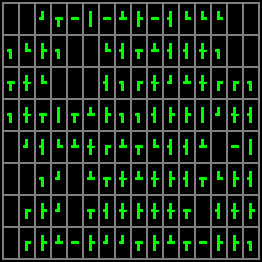
\includegraphics[scale=0.75]{\CURPATH/shuffled.png}
\caption{Shuffled puzzle}
\end{figure}

\dots and solved:

\begin{figure}[H]
\label{fig:pipe_solved}
\centering
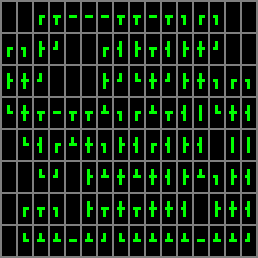
\includegraphics[scale=0.75]{\CURPATH/solved.png}
\caption{Solved puzzle}
\end{figure}

Let's try to find a way to solve it.

\subsubsection{Generation}

First, we need to generate it.
Here is my quick idea on it.
Take 8*16 array of cells.
Each cell may contain some type of block.
There are joints between cells:

\pgfmathsetmacro\Width{16}
\pgfmathsetmacro\Height{8}
%\pgfmathsetmacro\Width{10}
%\pgfmathsetmacro\Height{5}
\pgfmathtruncatemacro\WidthMinusI{\Width - 1}
\pgfmathtruncatemacro\WidthMinusII{\Width - 2}
\pgfmathtruncatemacro\HeightMinusI{\Height - 1}
\pgfmathtruncatemacro\HeightMinusII{\Height - 2}
\pgfmathtruncatemacro\HeightPlusII{\Height + 2}
\pgfmathsetmacro\HeightPlusIi{\Height + 1.5}

% see also: http://www.texample.net/tikz/examples/euclid-algorithm/
\begin{center}
\begin{tikzpicture}[set style={{help lines}+=[dashed]},scale=0.7]

	\draw[style=help lines] (0,0) grid +(\Width,\Height);

	\foreach \c in {0,...,\WidthMinusI}
	{
		\foreach \r in {0,...,\HeightMinusII}
			\draw   [red,very thick,-] (\c+0.5,\r+0.75) -- (\c+0.5,\r+1.25);
		%\node[rotate=90] at (\c+0.5,\HeightPlusII) {\Large vjoints[\dots, \c] \normalsize};
		\node[rotate=90] at (\c+0.5,\HeightPlusII) {vjoints[\dots, \c]};
	}

	\foreach \r in {0,...,\HeightMinusI}
	{
		\foreach \c in {0,...,\WidthMinusII}
			\draw   [blue,very thick,-] (\c+0.75,\r+0.5) -- (\c+1.25,\r+0.5);
		\pgfmathtruncatemacro\hjointslabel{\HeightMinusI - \r}
		%\node at (-1.5,\r+0.5) {\large hjoints[\hjointslabel, \dots] \normalsize};
		\node at (-1.5,\r+0.5) {hjoints[\hjointslabel, \dots]};
	}

\end{tikzpicture}
\end{center}



Blue lines are horizontal joints, red lines are vertical joints.
We just set each joint to 0/false (absent) or 1/true (present), randomly.

Once set, it's now easy to find type for each cell.
There are:

\newcommand{\HeaderColor}{\cellcolor{blue!25}}
\begin{center}
\begin{longtable}{ | l | l | l | l | }
\hline
\HeaderColor joints & \HeaderColor our internal name & \HeaderColor angle & \HeaderColor symbol \\
\hline
0	&type 0		&	0$^{\circ}$	& (space)	\\
2	&type 2a	&	0$^{\circ}$	& \pmboxdrawuni{2503} \\ % ┃
2	&type 2a	&	90$^{\circ}$	& \pmboxdrawuni{2501} \\ % ━
2	&type 2b	&	0$^{\circ}$	& \pmboxdrawuni{250F} \\ % ┏
2	&type 2b	&	90$^{\circ}$	& \pmboxdrawuni{2513} \\ % ┓
2	&type 2b	&	180$^{\circ}$	& \pmboxdrawuni{251B} \\ % ┛
2	&type 2b	&	270$^{\circ}$	& \pmboxdrawuni{2517} \\ % ┗
3	&type 3		&	0$^{\circ}$	& \pmboxdrawuni{2523} \\ % ┣
3 	&type 3		&	90$^{\circ}$	& \pmboxdrawuni{2533} \\ % ┳
3	&type 3		&	180$^{\circ}$	& \pmboxdrawuni{252B} \\ % ┫
3	&type 3		&	270$^{\circ}$	& \pmboxdrawuni{253B} \\ % ┻
4	&type 4		&	0$^{\circ}$	& \pmboxdrawuni{254B} \\ % ╋
\hline
\end{longtable}
\end{center}

\textit{Dangling} joints can be preset at a first stage (i.e., cell with only one joint), but they are removed recursively,
these cells are transforming into empty cells.
Hence, at the end, all cells has at least two joints, and the whole plumbing system has no connections with outer
world---I hope this would make things clearer.

The C source code of generator is here: \url{https://github.com/DennisYurichev/SAT_SMT_by_example/tree/master/puzzles/pipe/generator}.
All horizontal joints are stored in the global array \textit{hjoints[]} and vertical in \textit{vjoints[]}.

The C program generates ANSI-colored output like it has been showed above (\ref{fig:pipe_shuffled}, \ref{fig:pipe_solved}) plus
an array of types, with no angle information about each cell:

\begin{lstlisting}[label=init_cells]
[
["0", "0", "2b", "3", "2a", "2a", "2a", "3", "3", "2a", "3", "2b", "2b", "2b", "0", "0"],
["2b", "2b", "3", "2b", "0", "0", "2b", "3", "3", "3", "3", "3", "4", "2b", "0", "0"],
["3", "4", "2b", "0", "0", "0", "3", "2b", "2b", "4", "2b", "3", "4", "2b", "2b", "2b"],
["2b", "4", "3", "2a", "3", "3", "3", "2b", "2b", "3", "3", "3", "2a", "2b", "4", "3"],
["0", "2b", "3", "2b", "3", "4", "2b", "3", "3", "2b", "3", "3", "3", "0", "2a", "2a"],
["0", "0", "2b", "2b", "0", "3", "3", "4", "3", "4", "3", "3", "3", "2b", "3", "3"],
["0", "2b", "3", "2b", "0", "3", "3", "4", "3", "4", "4", "3", "0", "3", "4", "3"],
["0", "2b", "3", "3", "2a", "3", "2b", "2b", "3", "3", "3", "3", "2a", "3", "3", "2b"],
]
\end{lstlisting}

\subsubsection{Solving}

First of all, we would think about 8*16 array of cells, where each has four bits:
``T'' (top),
``B'' (bottom),
``L'' (left),
``R'' (right).
Each bit represents half of joint.

% see also: http://www.texample.net/tikz/examples/euclid-algorithm/
\begin{center}
\begin{tikzpicture}[set style={{help lines}+=[dashed]},scale=0.7]

	\draw[style=help lines] (0,0) grid +(\Width,\Height);
	
	\foreach \c in {0,...,\WidthMinusI}
		%\node[rotate=90] at (\c+0.5,\HeightPlusIi) {\Large [\dots, \c] \normalsize};
		\node[rotate=90] at (\c+0.5,\HeightPlusIi) {[\dots, \c]};
	
	\foreach \r in {0,...,\HeightMinusI}
	{
		\pgfmathtruncatemacro\hlabel{\HeightMinusI - \r}
		%\node at (-1.5,\r+0.5) {\large [\hlabel, \dots] \normalsize};
		\node at (-1.5,\r+0.5) {[\hlabel, \dots]};
	
		\pgfmathsetmacro\Shift{0.325}
		\foreach \c in {0,...,\WidthMinusI}
		{
			\node at (\c+0.5,\r+0.5 + \Shift) {\footnotesize T \normalsize};
			\node at (\c+0.5,\r+0.5 - \Shift) {\footnotesize B \normalsize};
			\node at (\c+0.5 - \Shift,\r+0.5) {\footnotesize L \normalsize};
			\node at (\c+0.5 + \Shift,\r+0.5) {\footnotesize R \normalsize};
		}
	}

\end{tikzpicture}
\end{center}


Now we define arrays of each of four half-joints + angle information:

\begin{lstlisting}
HEIGHT=8
WIDTH=16

# if T/B/R/L is Bool instead of Int, Z3 solver will work faster
T=[[Bool('cell_%d_%d_top' % (r, c)) for c in range(WIDTH)] for r in range(HEIGHT)]
B=[[Bool('cell_%d_%d_bottom' % (r, c)) for c in range(WIDTH)] for r in range(HEIGHT)]
R=[[Bool('cell_%d_%d_right' % (r, c)) for c in range(WIDTH)] for r in range(HEIGHT)]
L=[[Bool('cell_%d_%d_left' % (r, c)) for c in range(WIDTH)] for r in range(HEIGHT)]
A=[[Int('cell_%d_%d_angle' % (r, c)) for c in range(WIDTH)] for r in range(HEIGHT)]
\end{lstlisting}

We know that if each of half-joints is present, corresponding half-joint must be also present, and vice versa.
We define this using these constraints:

\begin{lstlisting}
# shorthand variables for True and False:
t=True
f=False

# "top" of each cell must be equal to "bottom" of the cell above
# "bottom" of each cell must be equal to "top" of the cell below
# "left" of each cell must be equal to "right" of the cell at left
# "right" of each cell must be equal to "left" of the cell at right
for r in range(HEIGHT):
    for c in range(WIDTH):
        if r!=0:
            s.add(T[r][c]==B[r-1][c])
        if r!=HEIGHT-1:
            s.add(B[r][c]==T[r+1][c])
        if c!=0:
            s.add(L[r][c]==R[r][c-1])
        if c!=WIDTH-1:
            s.add(R[r][c]==L[r][c+1])

# "left" of each cell of first column shouldn't have any connection
# so is "right" of each cell of the last column
for r in range(HEIGHT):
    s.add(L[r][0]==f)
    s.add(R[r][WIDTH-1]==f)

# "top" of each cell of the first row shouldn't have any connection
# so is "bottom" of each cell of the last row
for c in range(WIDTH):
    s.add(T[0][c]==f)
    s.add(B[HEIGHT-1][c]==f)
\end{lstlisting}

Now we'll enumerate all cells in the initial array (\ref{init_cells}).
First two cells are empty there. And the third one has type ``2b''.
This is ``\pmboxdrawuni{250F}'' % ┏
and it can be oriented in 4 possible ways.
And if it has angle 0$^{\circ}$, bottom and right half-joints are present, others are absent.
If it has angle 90$^{\circ}$, it looks like 
``\pmboxdrawuni{2513}'', % ┓
and bottom and left half-joints are present, others are absent.

In plain English: ``if cell of this type has angle 0$^{\circ}$, these half-joints must be present \textbf{OR}
if it has angle 90$^{\circ}$, these half-joints must be present, \textbf{OR}, etc, etc.''

Likewise, we define all these rules for all types and all possible angles:

\begin{lstlisting}
for r in range(HEIGHT):
    for c in range(WIDTH):
        ty=cells_type[r][c]

        if ty=="0":
            s.add(A[r][c]==f)
            s.add(T[r][c]==f, B[r][c]==f, L[r][c]==f, R[r][c]==f)

        if ty=="2a":
            s.add(Or(And(A[r][c]==0, L[r][c]==f, R[r][c]==f, T[r][c]==t, B[r][c]==t),   # §\pmboxdrawuni{2503}§
                    And(A[r][c]==90, L[r][c]==t, R[r][c]==t, T[r][c]==f, B[r][c]==f)))  # §\pmboxdrawuni{2501}§

        if ty=="2b":
            s.add(Or(And(A[r][c]==0, L[r][c]==f, R[r][c]==t, T[r][c]==f, B[r][c]==t),   # §\pmboxdrawuni{250F}§
                    And(A[r][c]==90, L[r][c]==t, R[r][c]==f, T[r][c]==f, B[r][c]==t),   # §\pmboxdrawuni{2513}§
                    And(A[r][c]==180, L[r][c]==t, R[r][c]==f, T[r][c]==t, B[r][c]==f),  # §\pmboxdrawuni{251B}§
                    And(A[r][c]==270, L[r][c]==f, R[r][c]==t, T[r][c]==t, B[r][c]==f))) # §\pmboxdrawuni{2517}§
	
        if ty=="3":
            s.add(Or(And(A[r][c]==0, L[r][c]==f, R[r][c]==t, T[r][c]==t, B[r][c]==t),   # §\pmboxdrawuni{2523}§
                    And(A[r][c]==90, L[r][c]==t, R[r][c]==t, T[r][c]==f, B[r][c]==t),   # §\pmboxdrawuni{2533}§
                    And(A[r][c]==180, L[r][c]==t, R[r][c]==f, T[r][c]==t, B[r][c]==t),  # §\pmboxdrawuni{252B}§
                    And(A[r][c]==270, L[r][c]==t, R[r][c]==t, T[r][c]==t, B[r][c]==f))) # §\pmboxdrawuni{253B}§

        if ty=="4":
            s.add(A[r][c]==0)
            s.add(T[r][c]==t, B[r][c]==t, L[r][c]==t, R[r][c]==t) # §\pmboxdrawuni{254B}§
\end{lstlisting}

Full source code is here: \url{https://github.com/DennisYurichev/SAT_SMT_by_example/blob/master/puzzles/pipe/solver/solve_pipe_puzzle1.py}.

It produces this result (prints angle for each cell and (pseudo)graphical representation):

\begin{figure}[H]
\centering
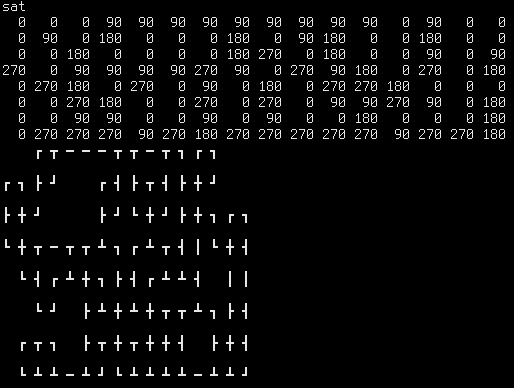
\includegraphics[scale=0.75]{\CURPATH/solver/solver.png}
\caption{Solver script output}
\end{figure}

It worked $\approx 4$ seconds on my old and slow Intel Atom N455 1.66GHz.
Is it fast? I don't know, but again, what is really cool, we do not know about any mathematical background
of all this, we just defined cells, (half-)joints and defined relations between them.

Now the next question is, how many solutions are possible?
Using method described earlier (\ref{SMTEnumerate}), I've altered solver script
\footnote{\url{https://github.com/DennisYurichev/SAT_SMT_by_example/blob/master/puzzles/pipe/solver/solve_pipe_puzzle2.py}} and solver
said two solutions are possible.

Let's compare these two solutions using gvimdiff:

\begin{figure}[H]
\centering
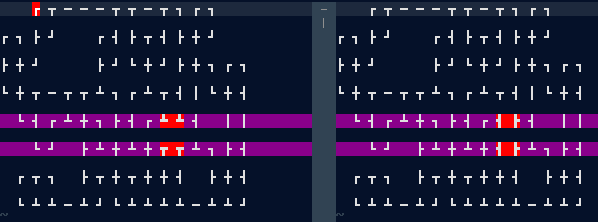
\includegraphics[scale=0.75]{\CURPATH/solver/diff.png}
\caption{gvimdiff output (pardon my red cursor at left pane at left-top corner)}
\end{figure}

4 cells in the middle can be orientated differently.
Perhaps, other puzzles may produce different results.

P.S.
\textit{Half-joint} is defined as boolean type.
But in fact, the first version of the solver has been written using integer type for half-joints,
and 0 was used for False and 1 for True.
I did it so because I wanted to make source code tidier and narrower without using long words like ``False'' and ``True''.
And it worked, but slower. Perhaps, Z3 handles boolean data types faster? Better?
Anyway, I writing this to note that integer type can also be used instead of boolean, if needed.


\section{Eight queens problem (SAT)}
\label{EightQueens}

\renewcommand{\CURPATH}{puzzles/8queens}

Eight queens is a very popular problem and often used for measuring performance of SAT solvers.
The problem is to place 8 queens on chess board so they will not attack each other.
For example:

\begin{lstlisting}
| | | |*| | | | |
| | | | | | |*| |
| | | | |*| | | |
| |*| | | | | | |
| | | | | |*| | |
|*| | | | | | | |
| | |*| | | | | |
| | | | | | | |*|
\end{lstlisting}

Let's try to figure out how to solve it.

\subsection{make\_one\_hot}
\label{POPCNTOne}

One important function we will (often) use is \TT{make\_one\_hot}.
This is a function which returns \textit{True} if one single of inputs is \textit{True} and others are \textit{False}.
It will return \textit{False} otherwise.

In my other examples, I've used Wolfram Mathematica to generate CNF clauses for it, for example: \ref{minesweeper_SAT}.
What expression Mathematica offers as \TT{make\_one\_hot} function with 8 inputs?

\begin{lstlisting}
(!a||!b)&&(!a||!c)&&(!a||!d)&&(!a||!e)&&(!a||!f)&&(!a||!g)&&(!a||!h)&&(a||b||c||d||e||f||g||h)&&
(!b||!c)&&(!b||!d)&&(!b||!e)&&(!b||!f)&&(!b||!g)&&(!b||!h)&&(!c||!d)&&(!c||!e)&&(!c||!f)&&(!c||!g)&&
(!c||!h)&&(!d||!e)&&(!d||!f)&&(!d||!g)&&(!d||!h)&&(!e||!f)&&(!e||!g)&&(!e||!h)&&(!f||!g)&&(!f||!h)&&(!g||!h)
\end{lstlisting}

We can clearly see that the expression constisting of all possible variable pairs (negated) plus
enumeration of all variables (non-negated).
In plain English terms, this means: ``no pair can be equal to two \textit{True}'s \textit{AND} at least one \textit{True}
must be present among all variables''.

This is how it works: if two variables will be \textit{True}, negated they will be both \textit{False},
and this clause will not be evaluated
to \textit{True}, which is our ultimate goal.
If one of variables is \textit{True}, both negated will produce one \textit{True} and one \textit{False} (fine).
If both variables are False, both negated will produce two \textit{True's} (again, fine).

Here is how I can generate clauses for the function using \textit{itertools} module from Python,
which provides many important functions from combinatorics:

\begin{lstlisting}
    # naive/pairwise encoding   
    def AtMost1(self, lst):
        for pair in itertools.combinations(lst, r=2):
            self.add_clause([self.neg(pair[0]), self.neg(pair[1])])
       
    # make one-hot (AKA unitary) variable
    def make_one_hot(self, lst):
        self.AtMost1(lst)
        self.OR_always(lst)
\end{lstlisting}

\TT{AtMost1()} function enumerates all possible pairs using \textit{itertools} function
\textit{combinations()}.

\TT{make\_one\_hot()} function does the same, but also adds a final clause, which forces at least one
\textit{True} variable to be present.

What clauses will be generated for 5 variables (1..5)?

\lstinputlisting{\CURPATH/popcnt1.cnf}

Yes, these are all possible pairs of 1..5 numbers + all 5 numbers.

We can get all solutions using Picosat:

\begin{lstlisting}
% picosat --all popcnt1.cnf

s SATISFIABLE
v -1 -2 -3 -4 5 0
s SATISFIABLE
v -1 -2 -3 4 -5 0
s SATISFIABLE
v -1 -2 3 -4 -5 0
s SATISFIABLE
v -1 2 -3 -4 -5 0
s SATISFIABLE
v 1 -2 -3 -4 -5 0
s SOLUTIONS 5
\end{lstlisting}

5 possible solutions indeed.

\subsection{Eight queens}

Now let's get back to eight queens.

We can assign 64 variables to $8 \cdot 8=64$ cells.
Cell occuppied with queen will be \textit{True}, vacant cell will be \textit{False}.

The problem of placing non-attacking (each other) queens on chess board (of any size) can be stated in plain English like this:
\begin{itemize}
\item one single queen must be present at each row;

\item one single queen must be present at each column;

\item zero or one queen must be present at each diagonal (empty diagonals can be present in valid solution).
\end{itemize}

These rules can be translated like that:

\begin{itemize}
\item make\_one\_hot(each row)==\textit{True}

\item make\_one\_hot(each column)==\textit{True}

\item AtMost1(each diagonal)==\textit{True}
\end{itemize}

Now all we need is to enumerate rows, columns and diagonals and gather all clauses:

\lstinputlisting[style=custompy]{\CURPATH/8queens.py}
( \url{https://github.com/DennisYurichev/SAT_SMT_by_example/blob/master/puzzles/8queens/8queens.py} )

Perhaps, \TT{gen\_diagonal()} function is not very aesthetically appealing: it enumerates also subdiagonals
of already enumerated longer diagonals.
To prevent presence of duplicate clauses, \textit{clauses} global variable is not a list, rather set, which allows
only unique data to be present there.

Also, I've used \TT{AtMost1} for each column, this will help to produce slightly lower number of clauses.
Each column will have a queen anyway, this is implied from the first rule (\TT{make\_one\_hot} for each row).

After running, we got CNF file with 64 variables and 736 clauses (\url{https://github.com/DennisYurichev/SAT_SMT_by_example/blob/master/puzzles/8queens/8queens.cnf}).
Here is one solution:

\begin{lstlisting}
% python 8queens.py
len(clauses)= 736
| | | |*| | | | |
| | | | | | |*| |
| | | | |*| | | |
| |*| | | | | | |
| | | | | |*| | |
|*| | | | | | | |
| | |*| | | | | |
| | | | | | | |*|
\end{lstlisting}

How many possible solutions are there?
Picosat tells 92, which is indeed correct number of solutions (\url{https://oeis.org/A000170}).

Performance of Picosat is not impressive, probably because it has to output all the solutions.
It took 34 seconds on my ancient Intel Atom 1.66GHz netbook to enumerate all solutions for $11 \cdot 11$ chess board
(2680 solutions),
which is way slower than my straigt brute-force program: \url{https://yurichev.com/blog/8queens/}.
Nevertheless, it's lighting fast (as other SAT solvers) in finding first solution.

The SAT instance is also small enough to be easily solved by my simplest possible backtracking SAT solver:
\ref{SAT_backtrack}.

\subsection{Counting all solutions}

We get a solution, negate it and add as a new constraint.
In plain English language this sounds ``find a solution, which is also can't be equal to the recently found/added''.
We add them consequently and the process is slowing---just because a problem (\textit{instance}) is growing and SAT solver
experience hard times in find yet another solution.

\subsection{Skipping symmetrical solutions}

We can also add rotated and reflected (horizontally) solution, so to skip symmetrical solutions.
By doing so, we're getting 12 solutions for 8*8 board, 46 for 9*9 board, etc.
This is \url{https://oeis.org/A002562}.


\section{Solving pocket Rubik’s cube (2*2*2) using Z3}
\label{PocketCubeSMT}

\renewcommand{\CURPATH}{puzzles/rubik2/failed_SMT}

\begin{figure}[H]
\centering
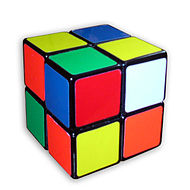
\includegraphics[scale=0.75]{\CURPATH/190px-Pocket_cube_scrambled.jpg}
\caption{Pocket cube}
\end{figure}

( The image has been taken \href{https://en.wikipedia.org/wiki/Pocket_Cube}{from Wikipedia}. )

Solving Rubik's cube is not a problem, finding shortest solution is.

\subsection{Intro}

First, a bit of terminology.
There are 6 colors we have: white, green, blue, orange, red, yellow.
We also have 6 sides: front, up, down, left, right, back.

This is how we will name all facelets:

% TODO TikZ
\begin{lstlisting}
        U1 U2
        U3 U4

       -------
L1 L2 | F1 F2 | R1 R2 | B1 B2
L3 L4 | F3 F4 | R3 R4 | B3 B4
       -------

        D1 D2
        D3 D4
\end{lstlisting}

Colors on a solved cube are:

\begin{lstlisting}
    G G
    G G
    ---
R R|W W|O O|Y Y
R R|W W|O O|Y Y
    ---
    B B
    B B
\end{lstlisting}

There are 6 possible turns: front, left, right, back, up, down.
But each turn can be clockwise, counterclockwise and half-turn (equal to two CW or two CCW).
Each CW is equal to 3 CCW and vice versa.
Hence, there are 6*3=18 possible turns.

It is known, that 11 turns (including half-turns) are enough to solve any pocket cube
(\href{https://en.wikipedia.org/wiki/Optimal_solutions_for_Rubik%27s_Cube}{God’s algorithm}).
This means, \href{http://mathworld.wolfram.com/GraphDiameter.html}{graph has a diameter} of 11.
For 3*3*3 cube one need 20 turns (\url{http://www.cube20.org/}).
See also: \url{https://en.wikipedia.org/wiki/Rubik%27s_Cube_group}.

\subsection{Z3}

There are 6 sides and 4 facelets on each, hence, 6*4=24 variables we need to define a state.

Then we define how state is transformed after each possible turn:

\begin{lstlisting}
FACE_F, FACE_U, FACE_D, FACE_R, FACE_L, FACE_B = 0,1,2,3,4,5

def rotate_FCW(s):
    return [
        [ s[FACE_F][2], s[FACE_F][0], s[FACE_F][3], s[FACE_F][1] ],   # for F
        [ s[FACE_U][0], s[FACE_U][1], s[FACE_L][3], s[FACE_L][1] ],   # for U
        [ s[FACE_R][2], s[FACE_R][0], s[FACE_D][2], s[FACE_D][3] ],   # for D
        [ s[FACE_U][2], s[FACE_R][1], s[FACE_U][3], s[FACE_R][3] ],   # for R
        [ s[FACE_L][0], s[FACE_D][0], s[FACE_L][2], s[FACE_D][1] ],   # for L
        [ s[FACE_B][0], s[FACE_B][1], s[FACE_B][2], s[FACE_B][3] ] ]  # for B

def rotate_FH(s):
    return [
        [ s[FACE_F][3], s[FACE_F][2], s[FACE_F][1], s[FACE_F][0] ],
        [ s[FACE_U][0], s[FACE_U][1], s[FACE_D][1], s[FACE_D][0] ],
        [ s[FACE_U][3], s[FACE_U][2], s[FACE_D][2], s[FACE_D][3] ],
        [ s[FACE_L][3], s[FACE_R][1], s[FACE_L][1], s[FACE_R][3] ],
        [ s[FACE_L][0], s[FACE_R][2], s[FACE_L][2], s[FACE_R][0] ],
        [ s[FACE_B][0], s[FACE_B][1], s[FACE_B][2], s[FACE_B][3] ] ]

...
\end{lstlisting}

Then we define a function, which takes turn number and transforms a state:

\begin{lstlisting}
# op is turn number
def rotate(turn, state, face, facelet):
    return If(op==0,  rotate_FCW (state)[face][facelet],
           If(op==1,  rotate_FCCW(state)[face][facelet],
           If(op==2,  rotate_UCW (state)[face][facelet],
           If(op==3,  rotate_UCCW(state)[face][facelet],
           If(op==4,  rotate_DCW (state)[face][facelet],

...

           If(op==17, rotate_BH  (state)[face][facelet],
                      0))))))))))))))))))
\end{lstlisting}

Now set "solved" state, initial state and connect everything:

\begin{lstlisting}
move_names=["FCW", "FCCW", "UCW", "UCCW", "DCW", "DCCW", "RCW", "RCCW", "LCW", "LCCW", "BCW", "BCCW", "FH", "UH", "DH", "RH", "LH", "BH"]

def colors_to_array_of_ints(s):
    return [{"W":0, "G":1, "B":2, "O":3, "R":4, "Y":5}[c] for c in s]

def set_current_state (d):
    F=colors_to_array_of_ints(d["FACE_F"])
    U=colors_to_array_of_ints(d["FACE_U"])
    D=colors_to_array_of_ints(d["FACE_D"])
    R=colors_to_array_of_ints(d["FACE_R"])
    L=colors_to_array_of_ints(d["FACE_L"])
    B=colors_to_array_of_ints(d["FACE_B"])
    return F,U,D,R,L,B # return tuple

# 4
init_F, init_U, init_D, init_R, init_L, init_B=set_current_state({"FACE_F":"RYOG", "FACE_U":"YRGO", "FACE_D":"WRBO", "FACE_R":"GYWB", "FACE_L":"BYWG", "FACE_B":"BOWR"})

...

for TURNS in range(1,12): # 1..11
    print "turns=", TURNS

    s=Solver()

    state=[[[Int('state%d_%d_%d' % (n, side, i)) for i in range(FACELETS)] for side in range(FACES)] for n in range(TURNS+1)]
    op=[Int('op%d' % n) for n in range(TURNS+1)]

    for i in range(FACELETS):
        s.add(state[0][FACE_F][i]==init_F[i])
        s.add(state[0][FACE_U][i]==init_U[i])
        s.add(state[0][FACE_D][i]==init_D[i])
        s.add(state[0][FACE_R][i]==init_R[i])
        s.add(state[0][FACE_L][i]==init_L[i])
        s.add(state[0][FACE_B][i]==init_B[i])

    # solved state
    for face in range(FACES):
        for facelet in range(FACELETS):
            s.add(state[TURNS][face][facelet]==face)

    # turns:
    for turn in range(TURNS):
        for face in range(FACES):
            for facelet in range(FACELETS):
                s.add(state[turn+1][face][facelet]==rotate(op[turn], state[turn], face, facelet))

    if s.check()==sat:
        print "sat"
        m=s.model()
        for turn in range(TURNS):
            print move_names[int(str(m[op[turn]]))]
        exit(0)
\end{lstlisting}

% FIXME URL
( The full source code: \url{https://github.com/DennisYurichev/SAT_SMT_by_example/blob/master/puzzles/rubik2/failed_SMT/rubik2_z3.py} )

That works:

\begin{lstlisting}
turns= 1
turns= 2
turns= 3
turns= 4
sat
RCW
UCW
DCW
RCW
\end{lstlisting}

...but very slow. It takes up to 1 hours to find a path of 8 turns, which is not enough, we need 11.

Nevetheless, I decided to include Z3 solver as a demonstration.


\subsection{Pocket Rubik's Cube (2*2*2) and SAT solver}
\label{PocketCubeSAT}.

\renewcommand{\CURPATH}{puzzles/rubik2/SAT}

I had success with my SAT-based solver, which can find an 11-turn path for a matter of 10-20 minutes on my old
Intel Xeon E3-1220 3.10GHz.

First, we will encode each color as 3-bit bit vector.
Then we can build electronic circuit, which will take initial state of cube and output final state.
It can have switches for each turn on each state.

% TODO TikZ
\begin{lstlisting}
                 +-----+    +-----+     +-----+
initial state -> | blk | -> | blk | ... | blk | -> final state
                 +-----+    +-----+     +-----+
                    ^          ^           ^
                    |          |           |
                  turn 1     turn 2    last turn
\end{lstlisting}

You set all turns and the device "calculates" final state.

Each "blk" can be constisted of 24 multiplexers (MUX), each for each facelet.
Each MUX is controlled by 5-bit command (turn number).
Depending on command, MUX takes 3-bit color from a facelet from a previous state.

Here is a table: the first column is a "destination" facelet, then a list of "source" facelets for each turn:

\begin{lstlisting}
    #      dst,  FCW  FH   FCCW UCW  UH   UCCW DCW  DH   DCCW RCW  RH   RCCW LCW  LH   LCCW BCW  BH   BCCW
    add_r("F1",["F3","F4","F2","R1","B1","L1","F1","F1","F1","F1","F1","F1","U1","B4","D1","F1","F1","F1"])
    add_r("F2",["F1","F3","F4","R2","B2","L2","F2","F2","F2","D2","B3","U2","F2","F2","F2","F2","F2","F2"])
    add_r("F3",["F4","F2","F1","F3","F3","F3","L3","B3","R3","F3","F3","F3","U3","B2","D3","F3","F3","F3"])
    add_r("F4",["F2","F1","F3","F4","F4","F4","L4","B4","R4","D4","B1","U4","F4","F4","F4","F4","F4","F4"])
    add_r("U1",["U1","U1","U1","U3","U4","U2","U1","U1","U1","U1","U1","U1","B4","D1","F1","R2","D4","L3"])
    add_r("U2",["U2","U2","U2","U1","U3","U4","U2","U2","U2","F2","D2","B3","U2","U2","U2","R4","D3","L1"])
    add_r("U3",["L4","D2","R1","U4","U2","U1","U3","U3","U3","U3","U3","U3","B2","D3","F3","U3","U3","U3"])
    add_r("U4",["L2","D1","R3","U2","U1","U3","U4","U4","U4","F4","D4","B1","U4","U4","U4","U4","U4","U4"])
    add_r("D1",["R3","U4","L2","D1","D1","D1","D3","D4","D2","D1","D1","D1","F1","U1","B4","D1","D1","D1"])
    add_r("D2",["R1","U3","L4","D2","D2","D2","D1","D3","D4","B3","U2","F2","D2","D2","D2","D2","D2","D2"])
    add_r("D3",["D3","D3","D3","D3","D3","D3","D4","D2","D1","D3","D3","D3","F3","U3","B2","L1","U2","R4"])
    add_r("D4",["D4","D4","D4","D4","D4","D4","D2","D1","D3","B1","U4","F4","D4","D4","D4","L3","U1","R2"])
    add_r("R1",["U3","L4","D2","B1","L1","F1","R1","R1","R1","R3","R4","R2","R1","R1","R1","R1","R1","R1"])
    add_r("R2",["R2","R2","R2","B2","L2","F2","R2","R2","R2","R1","R3","R4","R2","R2","R2","D4","L3","U1"])
    add_r("R3",["U4","L2","D1","R3","R3","R3","F3","L3","B3","R4","R2","R1","R3","R3","R3","R3","R3","R3"])
    add_r("R4",["R4","R4","R4","R4","R4","R4","F4","L4","B4","R2","R1","R3","R4","R4","R4","D3","L1","U2"])
    add_r("L1",["L1","L1","L1","F1","R1","B1","L1","L1","L1","L1","L1","L1","L3","L4","L2","U2","R4","D3"])
    add_r("L2",["D1","R3","U4","F2","R2","B2","L2","L2","L2","L2","L2","L2","L1","L3","L4","L2","L2","L2"])
    add_r("L3",["L3","L3","L3","L3","L3","L3","B3","R3","F3","L3","L3","L3","L4","L2","L1","U1","R2","D4"])
    add_r("L4",["D2","R1","U3","L4","L4","L4","B4","R4","F4","L4","L4","L4","L2","L1","L3","L4","L4","L4"])
    add_r("B1",["B1","B1","B1","L1","F1","R1","B1","B1","B1","U4","F4","D4","B1","B1","B1","B3","B4","B2"])
    add_r("B2",["B2","B2","B2","L2","F2","R2","B2","B2","B2","B2","B2","B2","D3","F3","U3","B1","B3","B4"])
    add_r("B3",["B3","B3","B3","B3","B3","B3","R3","F3","L3","U2","F2","D2","B3","B3","B3","B4","B2","B1"])
    add_r("B4",["B4","B4","B4","B4","B4","B4","R4","F4","L4","B4","B4","B4","D1","F1","U1","B2","B1","B3"])
\end{lstlisting}

Each MUX has 32 inputs, each has width of 3 bits: colors from "source" facelets.
It has 3-bit output (color for "destination" facelet).
It has 5-bit selector, for 18 turns. Other selector values (32-18=14 values) are not used at all.

The whole problem is to build a circuit and then ask SAT solver to set "switches" to such a state,
when input and output are determined (by us).

Now the problem is to represent MUX in CNF terms.

From \ac{EE} courses we can remember about a simple if-then-else (ITE) gate, it takes 3 inputs
("selector", "true" and "false") and it has 1 output.
Depending on "selector" input it "connects" output with "true" or "false" input.
Using tree of ITE gates we first can build 32-to-1 MUX, then wide 32*3-to-3 MUX.

% FIXME URL
I once have written small utility to search for shortest possible CNF formula for a specific function,
in a bruteforce manner (\url{.../XOR_CNF_bf.c}).
It was inspired by "aha! hacker assistant" by Henry Warren.
So here is a function:

\begin{lstlisting}
bool func(bool v[VARIABLES])
{

	// ITE:

	bool tmp;
	if (v[0]==0)
		tmp=v[1];
	else
		tmp=v[2];

	return tmp==v[3];
}
\end{lstlisting}

A shortest CNF for it:

\begin{lstlisting}
try_all_CNFs_of_len(1)
try_all_CNFs_of_len(2)
try_all_CNFs_of_len(3)
try_all_CNFs_of_len(4)
found a CNF:
p cnf 4 4
-1 3 -4 0
1 2 -4 0
-1 -3 4 0
1 -2 4 0
\end{lstlisting}

1st variable is "select", 2nd is "false", 3rd is "true", 4th is "output".
"output" is an additional variable, added just like in Tseitin transformations.

Hence, CNF formula is:

\begin{lstlisting}
(!select OR true OR !output) AND (select OR false OR !output) AND (!select OR !true OR output) AND (select OR !false OR output)
\end{lstlisting}

It assures that the "output" will always be equal to one of inputs depending on "select".

Now we can build a tree of \ac{ITE} gates:

\begin{lstlisting}
def create_ITE(s,f,t):
    x=create_var()

    clauses.append([neg(s),t,neg(x)])
    clauses.append([s,f,neg(x)])
    clauses.append([neg(s),neg(t),x])
    clauses.append([s,neg(f),x])

    return x

# ins=16 bits
# sel=4 bits
def create_MUX(ins, sel):
    t0=create_ITE(sel[0],ins[0],ins[1])
    t1=create_ITE(sel[0],ins[2],ins[3])
    t2=create_ITE(sel[0],ins[4],ins[5])
    t3=create_ITE(sel[0],ins[6],ins[7])
    t4=create_ITE(sel[0],ins[8],ins[9])
    t5=create_ITE(sel[0],ins[10],ins[11])
    t6=create_ITE(sel[0],ins[12],ins[13])
    t7=create_ITE(sel[0],ins[14],ins[15])

    y0=create_ITE(sel[1],t0,t1)
    y1=create_ITE(sel[1],t2,t3)
    y2=create_ITE(sel[1],t4,t5)
    y3=create_ITE(sel[1],t6,t7)

    z0=create_ITE(sel[2],y0,y1)
    z1=create_ITE(sel[2],y2,y3)

    return create_ITE(sel[3], z0, z1)
\end{lstlisting}

This is my old MUX I wrote for 16 inputs and 4-bit selector, but you've got the idea: this is 4-tier tree.
It has 15 ITE gates or 15*4=60 clauses.

Now the question, is it possible to make it smaller?
I've tried to use Mathematica.
First I've built truth table for 4-bit selector:

\begin{lstlisting}
...
1 1 1 1     1 1 1 1 1 1 0 1 0 1 0 1 1 0 1 1    0    0
1 1 1 1     1 1 1 1 1 1 0 1 0 1 0 1 1 0 1 1    1    1
1 1 1 1     1 1 1 1 1 1 0 1 0 1 0 1 1 1 0 0    0    0
1 1 1 1     1 1 1 1 1 1 0 1 0 1 0 1 1 1 0 0    1    1
1 1 1 1     1 1 1 1 1 1 0 1 0 1 0 1 1 1 0 1    0    0
1 1 1 1     1 1 1 1 1 1 0 1 0 1 0 1 1 1 0 1    1    1
1 1 1 1     1 1 1 1 1 1 0 1 0 1 0 1 1 1 1 0    0    0
1 1 1 1     1 1 1 1 1 1 0 1 0 1 0 1 1 1 1 0    1    1
1 1 1 1     1 1 1 1 1 1 0 1 0 1 0 1 1 1 1 1    0    0
1 1 1 1     1 1 1 1 1 1 0 1 0 1 0 1 1 1 1 1    1    1
1 1 1 1     1 1 1 1 1 1 0 1 0 1 1 0 0 0 0 0    0    0
1 1 1 1     1 1 1 1 1 1 0 1 0 1 1 0 0 0 0 0    1    1
1 1 1 1     1 1 1 1 1 1 0 1 0 1 1 0 0 0 0 1    0    0
1 1 1 1     1 1 1 1 1 1 0 1 0 1 1 0 0 0 0 1    1    1
1 1 1 1     1 1 1 1 1 1 0 1 0 1 1 0 0 0 1 0    0    0
1 1 1 1     1 1 1 1 1 1 0 1 0 1 1 0 0 0 1 0    1    1
1 1 1 1     1 1 1 1 1 1 0 1 0 1 1 0 0 0 1 1    0    0
...
\end{lstlisting}

First 4 bits is selector, then 16 bits of input.
Then the possible output and the bit, indicating, if the output bit equals to one of the inputs.

Then I load this table to Mathematica and make CNF expression out of truth table:

\begin{lstlisting}
arr=Import["/home/dennis/P/Rubik/TT","Table"]
{{0,0,0,0,0,0,0,0,0,0,0,0,0,0,0,0,0,0,0,0,0,1},{0,0,0,0,0,0,0,0,0,0,0,0,0,0,0,0,0,0,0,0,1,0},{0,0,0,0,0,0,0,0,0,0,0,0,0,0,0,0,0,0,0,1,0,0},
{0,0,0,0,0,0,0,0,0,0,0,0,0,0,0,0,0,0,0,1,1,1},{0,0,0,0,0,0,0,0,0,0,0,0,0,0,0,0,0,0,1,0,0,1},{0,0,0,0,0,0,0,0,0,0,0,0,0,0,0,0,0,0,1,0,1,0},
{0,0,0,0,0,0,0,0,0,0,0,0,0,0,0,0,0,0,1,1,0,0},{0,0,0,0,0,0,0,0,0,0,0,0,0,0,0,0,0,0,1,1,1,1},{0,0,0,0,0,0,0,0,0,0,0,0,0,0,0,0,0,1,0,0,0,1}, ⋯2097135⋯ ,
{1,1,1,1,1,1,1,1,1,1,1,1,1,1,1,1,1,1,0,0,0,0},{1,1,1,1,1,1,1,1,1,1,1,1,1,1,1,1,1,1,0,0,1,1},{1,1,1,1,1,1,1,1,1,1,1,1,1,1,1,1,1,1,0,1,0,0},
{1,1,1,1,1,1,1,1,1,1,1,1,1,1,1,1,1,1,0,1,1,1},{1,1,1,1,1,1,1,1,1,1,1,1,1,1,1,1,1,1,1,0,0,0},{1,1,1,1,1,1,1,1,1,1,1,1,1,1,1,1,1,1,1,0,1,1},
{1,1,1,1,1,1,1,1,1,1,1,1,1,1,1,1,1,1,1,1,0,0},{1,1,1,1,1,1,1,1,1,1,1,1,1,1,1,1,1,1,1,1,1,1}}


TT=(Most[#]->Last[#])&/@arr
{{0,0,0,0,0,0,0,0,0,0,0,0,0,0,0,0,0,0,0,0,0}->1,{0,0,0,0,0,0,0,0,0,0,0,0,0,0,0,0,0,0,0,0,1}->0,{0,0,0,0,0,0,0,0,0,0,0,0,0,0,0,0,0,0,0,1,0}->0,
{0,0,0,0,0,0,0,0,0,0,0,0,0,0,0,0,0,0,0,1,1}->1,{0,0,0,0,0,0,0,0,0,0,0,0,0,0,0,0,0,0,1,0,0}->1,{0,0,0,0,0,0,0,0,0,0,0,0,0,0,0,0,0,0,1,0,1}->0,
{0,0,0,0,0,0,0,0,0,0,0,0,0,0,0,0,0,0,1,1,0}->0,{0,0,0,0,0,0,0,0,0,0,0,0,0,0,0,0,0,0,1,1,1}->1,{0,0,0,0,0,0,0,0,0,0,0,0,0,0,0,0,0,1,0,0,0}->1, ⋯2097135⋯ ,
{1,1,1,1,1,1,1,1,1,1,1,1,1,1,1,1,1,1,0,0,0}->0,{1,1,1,1,1,1,1,1,1,1,1,1,1,1,1,1,1,1,0,0,1}->1,{1,1,1,1,1,1,1,1,1,1,1,1,1,1,1,1,1,1,0,1,0}->0,
{1,1,1,1,1,1,1,1,1,1,1,1,1,1,1,1,1,1,0,1,1}->1,{1,1,1,1,1,1,1,1,1,1,1,1,1,1,1,1,1,1,1,0,0}->0,{1,1,1,1,1,1,1,1,1,1,1,1,1,1,1,1,1,1,1,0,1}->1,
{1,1,1,1,1,1,1,1,1,1,1,1,1,1,1,1,1,1,1,1,0}->0,{1,1,1,1,1,1,1,1,1,1,1,1,1,1,1,1,1,1,1,1,1}->1}


BooleanConvert[BooleanFunction[TT,{s3,s2,s1,s0, i15,i14,i13,i12,i11,i10,i9,i8,i7,i6,i5,i4,i3, i2, i1, i0,x}],"CNF"]
(!i0||s0||s1||s2||s3||x)&&(i0||s0||s1||s2||s3||!x)&&(!i1||!s0||s1||s2||s3||x)&&(i1||!s0||s1||s2||s3||!x)&&(!i10||s0||!s1||s2||!s3||x)&&
(i10||s0||!s1||s2||!s3||!x)&&(!i11||!s0||!s1||s2||!s3||x)&&(i11||!s0||!s1||s2||!s3||!x)&&(!i12||s0||s1||!s2||!s3||x)&&(i12||s0||s1||!s2||!s3||!x)&&
(!i13||!s0||s1||!s2||!s3||x)&&(i13||!s0||s1||!s2||!s3||!x)&&(!i14||s0||!s1||!s2||!s3||x)&&(i14||s0||!s1||!s2||!s3||!x)&&
(!i15||!s0||!s1||!s2||!s3||x)&&(i15||!s0||!s1||!s2||!s3||!x)&&(!i2||s0||!s1||s2||s3||x)&&(i2||s0||!s1||s2||s3||!x)&&(!i3||!s0||!s1||s2||s3||x)&&
(i3||!s0||!s1||s2||s3||!x)&&(!i4||s0||s1||!s2||s3||x)&&(i4||s0||s1||!s2||s3||!x)&&(!i5||!s0||s1||!s2||s3||x)&&(i5||!s0||s1||!s2||s3||!x)&&
(!i6||s0||!s1||!s2||s3||x)&&(i6||s0||!s1||!s2||s3||!x)&&(!i7||!s0||!s1||!s2||s3||x)&&(i7||!s0||!s1||!s2||s3||!x)&&(!i8||s0||s1||s2||!s3||x)&&
(i8||s0||s1||s2||!s3||!x)&&(!i9||!s0||s1||s2||!s3||x)&&(i9||!s0||s1||s2||!s3||!x)
\end{lstlisting}

Look closer to CNF expression:

\begin{lstlisting}
(!i0|   |s0||s1||s2|| s3|| x)&&
( i0||  s0|| s1||s2|| s3||!x)&&
(!i1||! s0|| s1||s2|| s3|| x)&&
( i1||! s0|| s1||s2|| s3||!x)&&
(!i10|| s0||!s1||s2||!s3|| x)&&
( i10|| s0||!s1||s2||!s3||!x)&&
(!i11||!s0||!s1||s2||!s3|| x)&&
( i11||!s0||!s1||s2||!s3||!x)&&

...

(!i8|| s0||s1||s2||!s3|| x)&&
( i8|| s0||s1||s2||!s3||!x)&&
(!i9||!s0||s1||s2||!s3|| x)&&
( i9||!s0||s1||s2||!s3||!x)
\end{lstlisting}

It has simple structure and there are 32 clauses, against 60 in my previous attempt.
Will it work faster?
No, as my experience shows, it doesn't speed up anything.
Anyway, I used the latter idea to make MUX.

The following function makes pack of MUXes for each state, based on what I've got from Mathematica:

\begin{lstlisting}
    def create_MUX(self, ins, sels):
        assert 2**len(sels)==len(ins)
        x=self.create_var()
        for sel in range(len(ins)): # 32 for 5-bit selector
            tmp=[self.neg_if((sel>>i)&1==1, sels[i]) for i in range(len(sels))] # 5 for 5-bit selector
    
            self.add_clause([self.neg(ins[sel])] + tmp + [x])
            self.add_clause([ins[sel]] + tmp + [self.neg(x)])
        return x
    
    def create_wide_MUX (self, ins, sels):
        out=[]
        for i in range(len(ins[0])):
            inputs=[x[i] for x in ins]
            out.append(self.create_MUX(inputs, sels))
        return out
\end{lstlisting}

% FIXME URL to Xu.py

Now the function that glues all together:

\begin{lstlisting}
# src=list of 18 facelets
def add_r(dst, src):
    global facelets, selectors, s
    t=s.create_var()
    s.fix(t,True)
    for state in range(STATES-1):
        src_vectors=[]
        for tmp in src:
            src_vectors.append(facelets[state][tmp])

        # padding: there are 18 used MUX inputs, so add 32-18=14 for padding
        for i in range(32-18): 
            src_vectors.append([t,t,t])

        dst_vector=s.create_wide_MUX (src_vectors, selectors[state])
        s.fix_BV_EQ(dst_vector,facelets[state+1][dst])

...

    #      dst,  FCW  FH   FCCW UCW  UH   UCCW DCW  DH   DCCW RCW  RH   RCCW LCW  LH   LCCW BCW  BH   BCCW
    add_r("F1",["F3","F4","F2","R1","B1","L1","F1","F1","F1","F1","F1","F1","U1","B4","D1","F1","F1","F1"])
    add_r("F2",["F1","F3","F4","R2","B2","L2","F2","F2","F2","D2","B3","U2","F2","F2","F2","F2","F2","F2"])
    add_r("F3",["F4","F2","F1","F3","F3","F3","L3","B3","R3","F3","F3","F3","U3","B2","D3","F3","F3","F3"])
    add_r("F4",["F2","F1","F3","F4","F4","F4","L4","B4","R4","D4","B1","U4","F4","F4","F4","F4","F4","F4"])
    add_r("U1",["U1","U1","U1","U3","U4","U2","U1","U1","U1","U1","U1","U1","B4","D1","F1","R2","D4","L3"])
...
\end{lstlisting}

% FIXME URL
Now the full source code: \url{.../SAT.py}.
I tried to make it as concise as possible.
It requires minisat to be installed.

And it works up to 11 turns, starting at 11, then decreasing number of turns.
Here is an output for a state which can be solved with 4 turns:

\begin{lstlisting}
set_state(0, {"F":"RYOG", "U":"YRGO", "D":"WRBO", "R":"GYWB", "L":"BYWG", "B":"BOWR"})
\end{lstlisting}

\lstinputlisting{\CURPATH/post_RDUR.txt}

Even on my relic Intel Atom 1.5GHz netbook it takes just 20s.

You can find redundant turns in 11-turn solution, like double UH turns.
Of course, two UH turns returns the cube to the previous state.
So these "annihilating turns" are added if the final solution can be shorter.
Why the solver added it? There is no "no operation" turn. And the solver is forced to fit into 11 turns.
Hence, it do what it can to produce correct solution.

Now a hard example:

\begin{lstlisting}
set_state(0, {"F":"RORW", "U":"BRBB", "D":"GOOR", "R":"WYGY", "L":"OWYW", "B":"BYGG"})
\end{lstlisting}

\begin{lstlisting}
TURNS= 11
sat!
UCW
BCW
LCCW
BH
DCW
RH
DCCW
FCW
UH
LCW
RCW

TURNS= 10
sat!
RH
BCCW
LCCW
RH
BCCW
LH
BCW
DH
BCW
LCCW

...
\end{lstlisting}

( $\approx 5$ minutes on my old Intel Xeon E3-1220 3.10GHz. )

I couldn't find a pure "11-turn state" which is "unsat" for 10-turn, it seems, these are rare.
According to \href{https://en.wikipedia.org/wiki/Pocket_Cube}{wikipedia}, there are just 0.072\% of these states.
Like "20-turn states" for 3*3*3 cube, which are also rare.

\subsubsection{Several solutions}

According to picosat (--all option to get all possible solutions), the 4-turn example we just saw has 2 solutions.
Indeed, two consequent turns UCW and DCW can be interchanged, they do not conflict with each other.

\subsubsection{Other (failed) ideas}

Pocket cube (2*2*2) has no central facelets, so to solve it, you don't need to stick each color to each face.
Rather, you can define a constraint so that a colors on each face must be equal to each other.
Somehow, this slows down drastically my both Z3 and SAT-based solvers.

Also, to prevent "annihilating" turns, we can set a constraint so that each state cannot be equal to any of previous
states, i.e., states cannot repeat.
This also slows down my both solvers.

\subsubsection{3*3*3 cube}

3*3*3 cube requires much more turns (20), so I couldn't solve it with my methods.
I have success to solve maybe 10 or 11 turns.
But some people do all 20 turns: \href{https://arxiv.org/pdf/1105.1436.pdf}{Jingchao Chen}.

However, you can use 3*3*3 cube to play, because it can act as 2*2*2 cube: just use corners and ignore
edge and center cubes.
Here is mine I used, you can see that corners are correctly solved:

\begin{figure}[H]
\centering
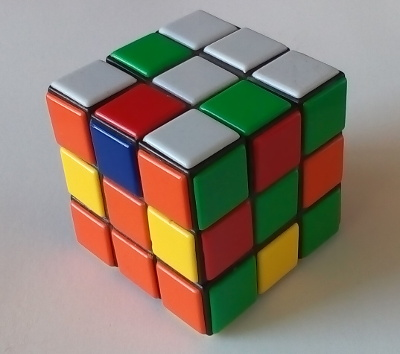
\includegraphics[scale=0.75]{\CURPATH/3solved.jpg}
\caption{Solved Rubik's cube as a pocket cube}
\end{figure}

\subsubsection{Some discussion}

\url{https://news.ycombinator.com/item?id=15214439},\\
\url{https://www.reddit.com/r/compsci/comments/6zb34i/solving_pocket_rubiks_cube_222_using_z3_and_sat/},\\
\url{https://www.reddit.com/r/Cubers/comments/6ze3ua/theory_dennis_yurichev_solving_pocket_rubiks_cube/}.


\section{Rubik’s cube (3*3*3) and Z3 SMT-solver}

As I wrote before, I couldn't solve even 2*2*2 pocket cube with Z3 (\ref{PocketCubeSMT}),
but I wanted to play with it further, and found
that it's still possible to solve one face instead of all 6.

I tried to model color of each facelet using integer sort (type), but now I can use bool: white facelet is True and all other non-white is False.
I can encode state of Rubik's cube like that: "W" for white facelet, "." for other.

Now the process of solving is a matter of minutes on a decent computer, or faster.

\begin{lstlisting}
#!/usr/bin/env python

from z3 import *

FACES=6
FACELETS=9

def rotate_FCW(s):
        return [
                [ s[0][6], s[0][3], s[0][0], s[0][7], s[0][4], s[0][1], s[0][8], s[0][5], s[0][2], ],  # new F
                [ s[1][0], s[1][1], s[1][2], s[1][3], s[1][4], s[1][5], s[4][8], s[4][5], s[4][2], ],  # new U
                [ s[3][6], s[3][3], s[3][0], s[2][3], s[2][4], s[2][5], s[2][6], s[2][7], s[2][8], ],  # new D
                [ s[1][6], s[3][1], s[3][2], s[1][7], s[3][4], s[3][5], s[1][8], s[3][7], s[3][8], ],  # new R
                [ s[4][0], s[4][1], s[2][0], s[4][3], s[4][4], s[2][1], s[4][6], s[4][7], s[2][2], ],  # new L
                [ s[5][0], s[5][1], s[5][2], s[5][3], s[5][4], s[5][5], s[5][6], s[5][7], s[5][8], ] ] # new B

def rotate_FH(s):
        return [
                [ s[0][8], s[0][7], s[0][6], s[0][5], s[0][4], s[0][3], s[0][2], s[0][1], s[0][0], ],
                [ s[1][0], s[1][1], s[1][2], s[1][3], s[1][4], s[1][5], s[2][2], s[2][1], s[2][0], ],
                [ s[1][8], s[1][7], s[1][6], s[2][3], s[2][4], s[2][5], s[2][6], s[2][7], s[2][8], ],
                [ s[4][8], s[3][1], s[3][2], s[4][5], s[3][4], s[3][5], s[4][2], s[3][7], s[3][8], ],
                [ s[4][0], s[4][1], s[3][6], s[4][3], s[4][4], s[3][3], s[4][6], s[4][7], s[3][0], ],
                [ s[5][0], s[5][1], s[5][2], s[5][3], s[5][4], s[5][5], s[5][6], s[5][7], s[5][8], ] ]


...


def rotate(op, st, side, j):
	return If(op==0, rotate_FCW(st)[side][j],
		If(op==1, rotate_FCCW(st)[side][j],
		If(op==2, rotate_UCW(st)[side][j],
		If(op==3, rotate_UCCW(st)[side][j],
		If(op==4, rotate_DCW(st)[side][j],
		If(op==5, rotate_DCCW(st)[side][j],
		If(op==6, rotate_RCW(st)[side][j],
		If(op==7, rotate_RCCW(st)[side][j],
		If(op==8, rotate_LCW(st)[side][j],
		If(op==9, rotate_LCCW(st)[side][j],
		If(op==10, rotate_BCW(st)[side][j],
		If(op==11, rotate_BCCW(st)[side][j],
		If(op==12, rotate_FH(st)[side][j],
		If(op==13, rotate_UH(st)[side][j],
		If(op==14, rotate_DH(st)[side][j],
		If(op==15, rotate_RH(st)[side][j],
		If(op==16, rotate_LH(st)[side][j],
		If(op==17, rotate_BH(st)[side][j],
			rotate_BH(st)[side][j], # default
			))))))))))))))))))

move_names=["FCW", "FCCW", "UCW", "UCCW", "DCW", "DCCW", "RCW", "RCCW", "LCW", "LCCW", "BCW", "BCCW", "FH", "UH", "DH", "RH", "LH", "BH"]

def colors_to_array_of_ints(s):
    rt=[]
    for c in s:
	if c=='W':
            rt.append(True)
        else:
            rt.append(False)
    return rt

def set_current_state (d):
    F=colors_to_array_of_ints(d["F"])
    U=colors_to_array_of_ints(d["U"])
    D=colors_to_array_of_ints(d["D"])
    R=colors_to_array_of_ints(d["R"])
    L=colors_to_array_of_ints(d["L"])
    B=colors_to_array_of_ints(d["B"])
    return F,U,D,R,L,B # return tuple

init_F, init_U, init_D, init_R, init_L, init_B=set_current_state({"F":"....W..W.", "U":"...W...W.", "D":".......W.", "R":"..W...W..", "L":"......W..", "B":"..W......"})

for STEPS in range(1, 20):
	print "trying %d steps" % STEPS

	s=Solver()
	state=[[[Bool('state%d_%d_%d' % (n, side, i)) for i in range(FACELETS)] for side in range(FACES)] for n in range(STEPS+1)]

	op=[Int('op%d' % n) for n in range(STEPS+1)]

	# initial state
	for i in range(FACELETS):
		s.add(state[0][0][i]==init_F[i])
		s.add(state[0][1][i]==init_U[i])
		s.add(state[0][2][i]==init_D[i])
		s.add(state[0][3][i]==init_R[i])
		s.add(state[0][4][i]==init_L[i])
		s.add(state[0][5][i]==init_B[i])

	# "must be" state for one (front/white) face
	for j in range(FACELETS):
		s.add(state[STEPS][0][j]==True)

	for n in range(STEPS):
		for side in range(FACES):
			for j in range(FACELETS):
				s.add(state[n+1][side][j]==rotate(op[n], state[n], side, j))

	if s.check()==sat:
		print "sat"
		m=s.model()
		for n in range(STEPS):
			print move_names[int(str(m[op[n]]))]
		exit(0)
\end{lstlisting}

( The full source code: \url{https://github.com/DennisYurichev/SAT_SMT_by_example/blob/master/puzzles/rubik3/one_face_SMT/rubik3_z3.py} )

\begin{lstlisting}
trying 1 steps
trying 2 steps
trying 3 steps
trying 4 steps
trying 5 steps
trying 6 steps
trying 7 steps
trying 8 steps
sat
LCW
UCCW
BCW
LCW
RCCW
BCCW
UCW
LCCW
\end{lstlisting}

Now the fun statistics.
Using random walk I collected 928 states and then I tried to solve one (white/front) face for each state.

\begin{lstlisting}
      1 turns= 4
      5 turns= 5
     57 turns= 6
    307 turns= 7
    501 turns= 8
     56 turns= 9
      1 turns= 10
\end{lstlisting}

It seems that majority of all states can be solved for 7-8 half turns (half-turn is one of 18 turns we used here).
But there is at least one state which must be solved with 10 half turns.
Maybe 10 is a "\href{http://www.cube20.org/}{god’s number}" for one face, like 20 for all 6 faces?


\subsection{Numberlink}
\label{numberlink}

\subsubsection{Numberlink (\ac{AKA} Flow Free) puzzle (Z3Py)}

You probably saw Flow Free puzzle:

\begin{figure}[H]
\centering
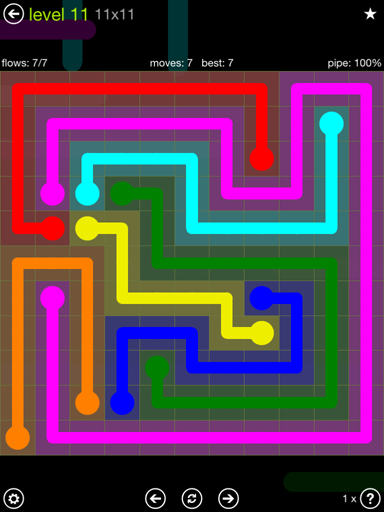
\includegraphics[scale=0.3]{puzzles/numberlink/Z3/flow-extreme-11-11.png}
\caption{}
\end{figure}

I'll stick to Numberlink version of the puzzle. This is the example puzzle from Wikipedia:

\begin{figure}[H]
\centering
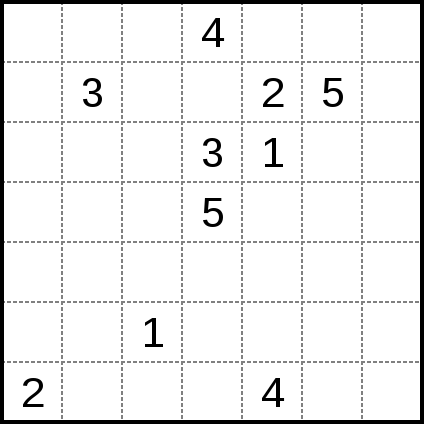
\includegraphics[scale=0.3]{puzzles/numberlink/Z3/424px-Numberlink_puzzle.png}
\caption{}
\end{figure}

This is solved:

\begin{figure}[H]
\centering
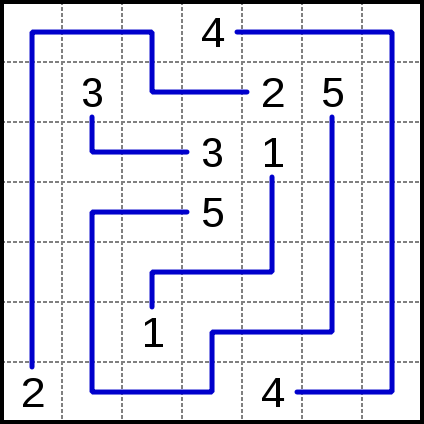
\includegraphics[scale=0.3]{puzzles/numberlink/Z3/424px-Numberlink_puzzle_solution.png}
\caption{}
\end{figure}

See also:
\url{https://en.wikipedia.org/wiki/Numberlink},
\url{https://en.wikipedia.org/wiki/Flow_Free}.

The code:

\lstinputlisting[style=custompy]{puzzles/numberlink/Z3/numberlink.py}

The solution:

\lstinputlisting{puzzles/numberlink/Z3/solution.txt}

\begin{figure}[H]
\centering
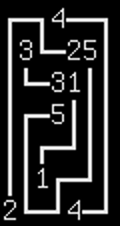
\includegraphics[scale=1]{puzzles/numberlink/Z3/solution.png}
\caption{The solution}
\end{figure}


\subsubsection{Numberlink (AKA Flow Free) puzzle as a MaxSAT problem + toy \ac{PCB} router}

% TODO \ref{}
Let's revisit my solution for Numberlink (AKA Flow Free) puzzle written for Z3Py.

What if holes in the puzzle exist?
Can we make all paths as short as possible?

I've rewritten the puzzle solver using my own SAT library 
and now I use \href{http://sat.inesc-id.pt/open-wbo/}{Open-WBO MaxSAT solver},
see the source code, which is almost the same: \url{https://github.com/DennisYurichev/SAT_SMT_by_example/blob/master/puzzles/numberlink/MaxSAT/numberlink_WBO.py}.

But now we ``maximize'' number of empty cells:

% TODO join these figures side-by-side:

\begin{figure}[H]
\centering
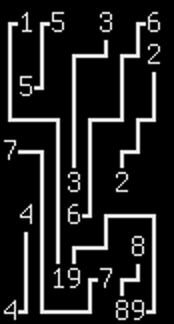
\includegraphics[scale=0.5]{puzzles/numberlink/MaxSAT/MaxSAT.png}
\caption{}
\end{figure}

This is a solution with shortest possible paths. Others are possible, but their sum wouldn't be shorter.
This is like toy \ac{PCB} routing.

What if we comment the \TT{s.fix\_soft\_always\_true(cell\_is\_empty[r][c], 1)} line and set \TT{maxsat=True}?

\begin{figure}[H]
\centering
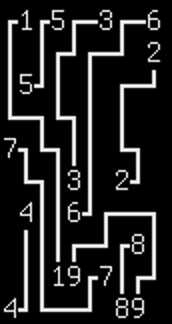
\includegraphics[scale=0.5]{puzzles/numberlink/MaxSAT/SAT.png}
\caption{}
\end{figure}

Lines 2 and 3 ``roaming'' chaotically, but the solution is correct, under given constraints.

The files: \url{https://github.com/DennisYurichev/SAT_SMT_by_example/tree/master/puzzles/numberlink/MaxSAT}.




\section{1959 AHSME Problems, Problem 6}

From \url{http://artofproblemsolving.com/wiki/index.php?title=1959_AHSME_Problems}:

\begin{framed}
\begin{quotation}

With the use of three different weights, namely $1$ lb., $3$ lb., and $9$ lb., 
how many objects of different weights can be weighed, if the objects is to be weighed 
and the given weights may be placed in either pan of the scale? 
15, 13, 11, 9, 7

\end{quotation}
\end{framed}

This is fun!

\begin{lstlisting}[style=custompy]
from z3 import *

# 0 - weight absent, 1 - on left pan, 2 - on right pan:
w1, w3, w9, obj = Ints('w1 w3 w9 obj')

obj_w = Int('obj_w')

s=Solver()

s.add(And(w1>=0, w1<=2))
s.add(And(w3>=0, w3<=2))
s.add(And(w9>=0, w9<=2))

# object is always on left or right pan:
s.add(And(obj>=1, obj<=2))

# object must weight something:
s.add(obj_w>0)

left, right = Ints('left right')

# left pan is a sum of weights/object, if they are present on pan:
s.add(left  == If(w1==1, 1, 0) + If(w3==1, 3, 0) + If(w9==1, 9, 0) + If(obj==1, obj_w, 0))
# same for right pan:
s.add(right == If(w1==2, 1, 0) + If(w3==2, 3, 0) + If(w9==2, 9, 0) + If(obj==2, obj_w, 0))

# both pans must weight something:
s.add(left>0)
s.add(right>0)

# pans must have equal weights:
s.add(left==right)

# get all results:
results=[]
while True:
    if s.check() == sat:
        m = s.model()
        #print m
        print "left: ",
        print ("w1" if m[w1].as_long()==1 else "  "),
        print ("w3" if m[w3].as_long()==1 else "  "),
        print ("w9" if m[w9].as_long()==1 else "  "),
        print (("obj_w=%2d" % m[obj_w].as_long()) if m[obj].as_long()==1 else "        "),

        print "    | right: ",
        print ("w1" if m[w1].as_long()==2 else "  "),
        print ("w3" if m[w3].as_long()==2 else "  "),
        print ("w9" if m[w9].as_long()==2 else "  "),
        print (("obj_w=%2d" % m[obj_w].as_long()) if m[obj].as_long()==2 else "        "),
        print ""

        results.append(m)
        block = []
        for d in m:
            # skip internal variables, do not add them to blocking constraint:
            if str(d).startswith ("z3name"):
                continue
            c=d()
            block.append(c != m[d])
        s.add(Or(block))
    else:
        print "total results", len(results)
        break
\end{lstlisting}

The output:

\begin{lstlisting}
left:     w3                 | right:  w1       obj_w= 2
left:     w3    obj_w= 7     | right:  w1    w9
left:     w3 w9              | right:  w1       obj_w=11
left:     w3    obj_w= 6     | right:        w9
left:  w1 w3    obj_w= 5     | right:        w9
left:     w3 w9              | right:           obj_w=12
left:  w1 w3 w9              | right:           obj_w=13
left:  w1 w3                 | right:           obj_w= 4
left:     w3                 | right:           obj_w= 3
left:           obj_w= 4     | right:  w1 w3
left:           obj_w=13     | right:  w1 w3 w9
left:           obj_w= 3     | right:     w3
left:  w1       obj_w= 2     | right:     w3
left:  w1       obj_w=11     | right:     w3 w9
left:           obj_w=12     | right:     w3 w9
left:  w1                    | right:           obj_w= 1
left:        w9              | right:  w1       obj_w= 8
left:        w9              | right:           obj_w= 9
left:  w1    w9              | right:           obj_w=10
left:  w1    w9              | right:     w3    obj_w= 7
left:        w9              | right:  w1 w3    obj_w= 5
left:        w9              | right:     w3    obj_w= 6
left:           obj_w= 9     | right:        w9
left:           obj_w=10     | right:  w1    w9
left:           obj_w= 1     | right:  w1
left:  w1       obj_w= 8     | right:        w9
total results 26
\end{lstlisting}

There are 13 distinct \TT{obj\_w} values. So this is the answer.


\subsection{Two parks}

The problem from the ``Discrete Structures, Logic and Computability'' book by James L. Hein, 4th ed.

\begin{framed}
\begin{quotation}

Suppose a survey revealed that 70\% of the population visited
an amusement park and 80\% visited a national park.
At least what percentage of the population visited both?

\end{quotation}
\end{framed}

The problem is supposed to be solved using finite sets counting...
But I'm slothful student and would try Z3.

\begin{lstlisting}[style=custompy]
from z3 import *

# each element is 0/1, reflecting 10% of park1/park2 levels of attendance...
p1=[Int('park1_%d' % i) for i in range(10)]
p2=[Int('park2_%d' % i) for i in range(10)]
# 1 if visited both, 0 otherwise:
b=[Int('both_%d' % i) for i in range(10)]

s=Optimize()
# sum of p1[] must be 7 (or 70%)
s.add(Sum(p1)==7)
# sum of p2[] must be 8 (or 80%)
s.add(Sum(p2)==8)

for i in range(10):
    # all in limits:
    s.add(And(p1[i]>=0, p1[i]<=1))
    s.add(And(p2[i]>=0, p2[i]<=1))
    # if both p1[] and p2[] has 1, b[] would have 1 as well:
    s.add(b[i]==If(And(p1[i]==1, p2[i]==1), 1, 0))

both=Int('both')
s.add(Sum(b)==both)

s.minimize(both)
#s.maximize(both)
assert s.check()==sat
m=s.model()

print "park1 : "+"".join([("*" if m[p1[i]].as_long()==1 else ".") for i in range(10)])
print "park2 : "+"".join([("*" if m[p2[i]].as_long()==1 else ".") for i in range(10)])
print "both  : "+"".join([("*" if m[b[i]].as_long()==1 else ".") for i in range(10)])+" (%d)" % m[both].as_long()
\end{lstlisting}

This is fun!

If minimize:

\begin{lstlisting}
park1 : ***...****
park2 : *..*******
both  : *.....**** (5)
\end{lstlisting}

If maximize:

\begin{lstlisting}
park1 : ..*******.
park2 : ..********
both  : ..*******. (7)
\end{lstlisting}

In other words, ``stars'' are allocated in such a way, so that the sum of ``stars'' in \TT{b[]} would be minimal/maximal.

Observing this, we can deduce the general formula:

Maximal both = min(park1, park2)

What about minimal both?
We can see that ``stars'' from one park1 must ``shift out'' or ``hide in'' to what corresponding empty space of park2.
So, minimal both = park2 - (100\% - park1)

SMT solver is overkill for the job, but perfect for illustration and helping in better understanding.

\subsubsection{Variations of the problem from the same book}

\begin{framed}
\begin{quotation}

Suppose that 100 senators voted on three separate senate bills as follows:
70 percent of the senators voted for the first bill, 65 percent voted for the second bill,
and 60 percent voted for the third bill. At least what percentage of the senators voted for all three bills?

\end{quotation}
\end{framed}

\begin{framed}
\begin{quotation}

Suppose that 25 people attended a conference with three sessions, where 15 people attended the first session, 
18 the second session, and 12 the third session. At least how many people attended all three sessions?

\end{quotation}
\end{framed}


\section{Alphametics}

According to Donald Knuth, the term ``Alphametics'' was coined by J. A. H. Hunter.
This is a puzzle: what decimal digits in 0..9 range must be assigned to each letter,
so the following equation will be true?

\begin{lstlisting}
  SEND
+ MORE
 -----
 MONEY
\end{lstlisting}

So is easy for Z3:

\lstinputlisting[style=custompy]{puzzles/alphametics/alpha.py}

Output:

\begin{lstlisting}
sat
[E, = 5,
 S, = 9,
 M, = 1,
 N, = 6,
 D, = 7,
 R, = 8,
 O, = 0,
 Y = 2]
\end{lstlisting}

Another one, also from \ac{TAOCP} volume IV (\url{http://www-cs-faculty.stanford.edu/~uno/fasc2b.ps.gz}):

\lstinputlisting[style=custompy]{puzzles/alphametics/alpha2.py}

\begin{lstlisting}
sat
[L, = 6,
 S, = 7,
 N, = 2,
 T, = 1,
 I, = 5,
 V = 3,
 A, = 8,
 R, = 9,
 O, = 4,
 TRIO = 1954,
 SONATA, = 742818,
 VIOLA, = 35468,
 VIOLIN, = 354652]
\end{lstlisting}

This puzzle I've found in pySMT examples\footnote{\url{http://pysmt.readthedocs.io/en/latest/getting_started.html}}:

\lstinputlisting[style=custompy]{puzzles/alphametics/alpha3.py}

\begin{lstlisting}
sat
[D = 5, R = 4, O = 3, E = 8, L = 6, W = 7, H = 2]
\end{lstlisting}

%%% 

This is an exercise Q209 from the 
[Companion to the Papers of Donald Knuth]\footnote{\url{http://www-cs-faculty.stanford.edu/~knuth/cp.html}}.

\begin{lstlisting}
 KNIFE
  FORK
 SPOON
  SOUP
------
SUPPER
\end{lstlisting}

I've added a helper function (list\_to\_expr()) to make things simpler:

\lstinputlisting[style=custompy]{puzzles/alphametics/alpha4.py}

\begin{lstlisting}
sat
[K = 7,
 N = 4,
 R = 9,
 I = 1,
 E = 6,
 S = 0,
 O = 3,
 F = 5,
 U = 8,
 P = 2,
 SUPPER = 82269,
 SOUP = 382,
 SPOON = 2334,
 FORK = 5397,
 KNIFE = 74156]
\end{lstlisting}

S is zero, so SUPPER value is starting with leading (removed) zero. Let's say, we don't like it. Add this to resolve it:

\begin{lstlisting}
s.add(S!=0)
\end{lstlisting}

\begin{lstlisting}
sat
[K = 8,
 N = 4,
 R = 3,
 I = 7,
 E = 6,
 S = 1,
 O = 9,
 F = 2,
 U = 0,
 P = 5,
 SUPPER = 105563,
 SOUP = 1905,
 SPOON = 15994,
 FORK = 2938,
 KNIFE = 84726]
\end{lstlisting}

\subsubsection{Devising your own puzzle}

Here is a problem: you can only use 10 letters, but how to select them among words?
We can try to offload this task to Z3:

\lstinputlisting[style=custompy]{puzzles/alphametics/gen.py}

This is the first generated puzzle:

\begin{lstlisting}
sat
EGGS
JELLY
LUNCH
C 5
E 6
G 3
H 7
J 0
L 1
N 4
S 8
U 2
Y 9
\end{lstlisting}

What if we want ``CAKE'' to be present among ``addends''?

Add this:

\begin{lstlisting}
s.add(word_used[words.index('CAKE')])
\end{lstlisting}

\begin{lstlisting}
sat
CAKE
TEA
LUNCH
A 8
C 3
E 1
H 9
J 6
K 2
L 0
N 5
T 7
U 4
\end{lstlisting}

Add this:

\begin{lstlisting}
s.add(word_used[words.index('EGGS')])
\end{lstlisting}

Now it can find pair to EGGS:

\begin{lstlisting}
sat
EGGS
HONEY
LUNCH
C 6
E 7
G 9
H 4
L 5
N 8
O 2
S 3
U 0
Y 1
\end{lstlisting}

\subsubsection{The files}

\url{https://github.com/DennisYurichev/SAT_SMT_by_example/tree/master/puzzles/alphametics}.



\section{2015 AIME II Problems/Problem 12}

At \url{http://artofproblemsolving.com/wiki/index.php?title=2015_AIME_II_Problems/Problem_12}:

\begin{framed}
\begin{quotation}
There are $2^{10} = 1024$ possible 10-letter strings in which each letter is either an A or a B.
Find the number of such strings that do not have more than 3 adjacent letters that are identical. 
\end{quotation}
\end{framed}

We just find all 10-bit numbers, which don't have 4-bit runs of zeros or ones:

\begin{lstlisting}
from z3 import *

a = BitVec('a', 10)

s=Solver()

for i in range(10-4+1):
    s.add(((a>>i)&15)!=0)
    s.add(((a>>i)&15)!=15)

results=[]
while True:
    if s.check() == sat:
        m = s.model()
        print "0x%x" % m[a].as_long()

        results.append(m)
        block = []
        for d in m:
            c=d()
            block.append(c != m[d])
        s.add(Or(block))
    else:
        print "total results", len(results)
        break
\end{lstlisting}

It's 548.


\subsection{Fred puzzle}

Found this:

\begin{lstlisting}
Three fellows accused of stealing CDs make the following statements:

(1) Ed: “Fred did it, and Ted is innocent.”
(2) Fred: “If Ed is guilty, then so is Ted.”
(3) Ted: “I’m innocent, but at least one of the others is guilty.”

If the innocent told the truth and the guilty lied, who is guilty? (Remember that false statements imply anything).

I think Ed and Ted are innocent and Fred is guilty. Is it in contradiction with statement 2.

What do you say?
\end{lstlisting}

( \url{https://math.stackexchange.com/questions/15199/implication-of-three-statements} )

And how to convert this into logic statements:

\begin{lstlisting}
Let us write the following propositions:

Fg means Fred is guilty, and Fi means Fred is innocent, Tg and Ti for Ted and Eg and Ei for Ed.

1. Ed says: Fg §$\wedge$§ Ti
2. Fred says: Eg §$\rightarrow$§ Tg
3. Ted says: Ti §$\wedge$§ (Fg §$\vee$§ Eg)

We know that the guilty is lying and the innocent tells the truth.

...

\end{lstlisting}

This is how I can implement it using Z3Py:

\lstinputlisting[style=custompy]{puzzles/fred/fred.py}

The result:

\begin{lstlisting}
sat
[fg = False,
 ti = False,
 tg = True,
 eg = True,
 ei = False,
 fi = True]
\end{lstlisting}

(Fred is innocent, others are guilty.)

(\TT{Implies} can be replaced with \TT{Or(Not(x), y)}.)

Now in SMT-LIB v2 form:

\lstinputlisting[style=customsmt]{puzzles/fred/fred.smt2}

Again, it's small enought to be solved by MK85:

\begin{lstlisting}
$ MK85 --dump-internal-variables fred.smt2
sat
(model
        (define-fun always_false () Bool false) ; var_no=1
        (define-fun always_true () Bool true) ; var_no=2
        (define-fun fg () Bool false) ; var_no=3
        (define-fun fi () Bool true) ; var_no=4
        (define-fun tg () Bool true) ; var_no=5
        (define-fun ti () Bool false) ; var_no=6
        (define-fun eg () Bool true) ; var_no=7
        (define-fun ei () Bool false) ; var_no=8
        (define-fun internal!1 () Bool true) ; var_no=9
        (define-fun internal!2 () Bool false) ; var_no=10
        (define-fun internal!3 () Bool true) ; var_no=11
        (define-fun internal!4 () Bool true) ; var_no=12
        (define-fun internal!5 () Bool false) ; var_no=13
        (define-fun internal!6 () Bool true) ; var_no=14
        (define-fun internal!7 () Bool true) ; var_no=15
        (define-fun internal!8 () Bool false) ; var_no=16
        (define-fun internal!9 () Bool true) ; var_no=17
        (define-fun internal!10 () Bool false) ; var_no=18
        (define-fun internal!11 () Bool false) ; var_no=19
        (define-fun internal!12 () Bool true) ; var_no=20
        (define-fun internal!13 () Bool false) ; var_no=21
        (define-fun internal!14 () Bool true) ; var_no=22
        (define-fun internal!15 () Bool false) ; var_no=23
        (define-fun internal!16 () Bool true) ; var_no=24
        (define-fun internal!17 () Bool true) ; var_no=25
        (define-fun internal!18 () Bool false) ; var_no=26
        (define-fun internal!19 () Bool false) ; var_no=27
        (define-fun internal!20 () Bool true) ; var_no=28
)
\end{lstlisting}

What is in the CNF file generated by MK85?

\lstinputlisting{puzzles/fred/tmp.cnf}

Let's filter out comments:

\lstinputlisting{puzzles/fred/tmp.cnf.comments}

% TODO \ref{}
Again, this instance is small enough to be solved by small backtracking SAT-solver:

\begin{lstlisting}
$ python SAT_backtrack.py tmp.cnf
SAT
-1 2 -3 4 5 -6 7 -8 9 -10 11 12 -13 14 15 -16 17 -18 -19 20 -21 22 -23 24 25 -26 -27 28 0
UNSAT
solutions= 1
\end{lstlisting}


\subsection{Multiple choice logic puzzle}

The source of this puzzle is probably Ross Honsberger's ``More Mathematical Morsels (Dolciani Mathematical Expositions)'' book:

\begin{lstlisting}
A certain question has the following possible answers.

    a. All of the below
    b. None of the below
    c. All of the above
    d. One of the above
    e. None of the above
    f. None of the above

Which answer is correct?
\end{lstlisting}

Cited from: \url{https://www.johndcook.com/blog/2015/07/06/multiple-choice/}.

This problem can be easily represented as a system of boolean equations.
Let's try to solve it using Z3. Each bool represents if the specific sentence is true.

\lstinputlisting[style=custompy]{puzzles/MC/mc.py}

The answer:

\begin{lstlisting}
sat
[f = False,
 b = False,
 a = False,
 c = False,
 d = False,
 e = True]
\end{lstlisting}

I can also rewrite this in SMT-LIB v2 form:

\lstinputlisting[style=custompy]{puzzles/MC/mc.smt2}

The problem is easy enough to be solved using MK85:

\begin{lstlisting}
sat
(model
        (define-fun a () Bool false)
        (define-fun b () Bool false)
        (define-fun c () Bool false)
        (define-fun d () Bool false)
        (define-fun e () Bool true)
        (define-fun f () Bool false)
)
\end{lstlisting}

Now let's have fun and see how my solver tackles this example.
What internal variables it creates?

\lstinputlisting{puzzles/MC/dbg1.txt}

What is in resulting CNF file to be fed into the external minisat SAT-solver?

\lstinputlisting{puzzles/MC/tmp.cnf}

Here are comments (starting with ``c '' prefix), and my SMT-solver indicate, how each low-level logical gate is added,
its inputs (variable IDs and numbers) and outputs.

Let's filter comments:

\lstinputlisting{puzzles/MC/tmp.cnf.comments}

Now you can juxtapose list of internal variables and comments in CNF file.
For example, equality gate is generated as NOT(XOR(a,b)).

create\_assert() function fixes a bool variable to always be True.

Other (internal) variables are added by SMT solver as ``joints'' to connect logic gates with each other.

Hence, my SMT solver constructing a digital circuit based on the input SMT file.
Logic gates are then converted into CNF form using Tseitin transformations.
The task of SAT solver is then to find such an assignment, for which CNF expression would be true.
In other words, its task is to find such inputs/outputs for which this ``virtual'' digital circuit would work
without contradictions.

% TODO \ref{}
The SAT instance is also small enough to be solved using my simplest backtracking SAT solver written:

\begin{lstlisting}
$ ./SAT_backtrack.py tmp.cnf

SAT
-1 2 -3 -4 -5 -6 7 -8 -9 -10 -11 -12 -13 14 15 16 17 -18 -19 20 -21 -22 23 -24 -25 26 27 -28 29 -30 31 -32 33 -34 -35 36 37 38 -39 -40 -41 42 43 44 45 46 47 48 49 -50 51 52 53 54 55 56 57 58 -59 -60 -61 62 0
UNSAT
solutions= 1
\end{lstlisting}

You can juxtapose variables from solver's result and variable numbers from MK85 listing.
Therefore, MK85 + my small SAT solver is standalone program under ~3000 SLOC, which still can solve such (simple enough) system of boolean equations, without external aid like minisat/picosat.

***

Among \href{https://www.johndcook.com/blog/2015/07/06/multiple-choice/}{comments} at the John D. Cook's blog, there is also a solution by Aaron Meurer, using SymPy,
which also has SAT-solver inside:

\begin{lstlisting}
7 July 2015 at 01:34

Decided to run this through SymPy’s SAT solver.

In [1]: var(‘a b c d e f’)
Out[1]: (a, b, c, d, e, f)

In [2]: facts = [
Equivalent(a, (b & c & d & e & f)),
Equivalent(b, (~c & ~d & ~e & ~f)),
Equivalent(c, a & b),
Equivalent(d, ((a & ~b & ~c) | (~a & b & ~c) | (~a & ~b & c))),
Equivalent(e, (~a & ~b & ~c & ~d)),
Equivalent(f, (~a & ~b & ~c & ~d & ~e)),
]

In [3]: list(satisfiable(And(*facts), all_models=True))
Out[3]: [{e: True, c: False, b: False, a: False, f: False, d: False}]

So it seems e is the only answer, assuming I got the facts correct. And it is important to use Equivalent (a bidirectional implication) rather than just Implies. If you only use -> (which I guess would mean that an answer not being chosen doesn’t necessarily mean that it isn’t true), then ‘none’, b, and f are also “solutions”.

Also, if I replace the d fact with Equivalent(d, a | b | c), the result is the same. So it seems that the interpretation of “one” both in terms of choice d and in terms of how many choices there are is irrelevant.

Thanks for the fun problem. I hope others took the time to solve this in their head before reading the comments.
\end{lstlisting}


\section{Coin flipping problem}
\label{coin_flip}

Found this on reddit:

\begin{lstlisting}
Coin flipping problem (KOI '06) (self.algorithms)

Hi. I'm struggling on this problem for weeks.

There is no official solution for this Korean Olympiad in Informatics problem.

The input is N × N coin boards, (0 < N < 33) 'H' means the coin's head is facing upward, and 'T' means the tail is facing upward.

The problem is minimizing T-coins with some operations:

    Flip all the coins in the same row.
    Flip all the coins in the same column.

Naïve O(N*2N) algorithm makes TLE. There are some heuristic approaches (Simulated Annealing) and branch-and-cut algorithm which reduces running time to about 200ms, but I have no idea to solve this problem in poly-time, or reduce this problem to any famous NP-complete problem.

Would you give some idea for me?
\end{lstlisting}

( \url{https://www.reddit.com/r/algorithms/comments/7aq9if/coin_flipping_problem_koi_06/} )

My solution for Z3:

\lstinputlisting[style=custompy]{puzzles/coin_flip/coin_z3.py}

Results:

\lstinputlisting{puzzles/coin_flip/z3.txt}

And also MaxSAT solution (Open-WBO MaxSAT solver): 

\lstinputlisting[style=custompy]{puzzles/coin_flip/coin_MaxSAT.py}

Results:

\lstinputlisting{puzzles/coin_flip/SAT.txt}

4-5 row/column flips can be achieved using this on 8*8 board (like chessboard) in reasonable time (couple of minutes).


\section{Lucky tickets}

It's quite popular meme in ex-USSR countries: ``lucky'' ticket is a ticket, which 6-digit number has the following property:
sum of the first 3 digits equals to the sum of the last 3 digits.

How many ``lucky'' tickets exists?

\lstinputlisting[style=customsmt]{puzzles/lucky_tickets/lucky_tickets.smt}


\subsection{Art of problem solving}

\url{http://artofproblemsolving.com/wiki/index.php?title=Mock_AIME_2_2006-2007_Problems/Problem_8}:

\begin{framed}
\begin{quotation}
The positive integers $x_1, x_2, ... , x_7$ satisfy $x_6 = 144$ and $x_{n+3} = x_{n+2}(x_{n+1}+x_n)$ for $n = 1, 2, 3, 4$. Find the last three digits of $x_7$.
\end{quotation}
\end{framed}

This is it:

\begin{lstlisting}[style=custompy]
from z3 import *

s=Solver()

x1, x2, x3, x4, x5, x6, x7=Ints('x1 x2 x3 x4 x5 x6 x7')

s.add(x1>=0)
s.add(x2>=0)
s.add(x3>=0)
s.add(x4>=0)
s.add(x5>=0)
s.add(x6>=0)
s.add(x7>=0)

s.add(x6==144)

s.add(x4==x3*(x2+x1))
s.add(x5==x4*(x3+x2))
s.add(x6==x5*(x4+x3))
s.add(x7==x6*(x5+x4))

# get all results:

results=[]
while True:
    if s.check() == sat:
        m = s.model()
        print m

        results.append(m)
        block = []
        for d in m:
            c=d()
            block.append(c != m[d])
        s.add(Or(block))
    else:
        print "total results", len(results)
        break
\end{lstlisting}

Two solutions possible, but in both x7 is ending by 456:

\begin{lstlisting}
[x2 = 1,
 x3 = 1,
 x1 = 7,
 x4 = 8,
 x5 = 16,
 x7 = 3456,
 x6 = 144]
[x3 = 2,
 x2 = 1,
 x1 = 2,
 x6 = 144,
 x4 = 6,
 x5 = 18,
 x7 = 3456]
total results 2
\end{lstlisting}


\section{2012 AIME I Problems/Problem 1}

\url{http://artofproblemsolving.com/wiki/index.php?title=2012_AIME_I_Problems/Problem_1}

\begin{framed}
\begin{quotation}

Find the number of positive integers with three not necessarily distinct digits,
$abc$, with $a \neq 0$ and $c \neq 0$ such that both $abc$ and $cba$ are multiples of $4$.

\end{quotation}
\end{framed}

\begin{lstlisting}[style=custompy]
from z3 import *

a, b, c = Ints('a b c')

s=Solver()

s.add(a>0)
s.add(b>=0)
s.add(c>0)

s.add(a<=9)
s.add(b<=9)
s.add(c<=9)

s.add((a*100 + b*10 + c) % 4 == 0)
s.add((c*100 + b*10 + a) % 4 == 0)

results=[]
while True:
    if s.check() == sat:
        m = s.model()
        print m

        results.append(m)
        block = []
        for d in m:
            c=d()
            block.append(c != m[d])
        s.add(Or(block))
    else:
        print "total results", len(results)
        break
\end{lstlisting}

Let's see:

\begin{lstlisting}
[c = 4, b = 0, a = 4]
[b = 1, c = 2, a = 2]
[b = 6, c = 4, a = 4]
[b = 4, c = 4, a = 4]
[b = 2, c = 4, a = 4]
[b = 4, c = 4, a = 8]
[b = 8, c = 4, a = 4]
[b = 6, c = 4, a = 8]
[b = 8, c = 4, a = 8]
[b = 0, c = 4, a = 8]
[b = 2, c = 4, a = 8]
[b = 8, c = 8, a = 8]
[b = 9, c = 6, a = 6]
[b = 2, c = 8, a = 8]
[b = 2, c = 8, a = 4]
[b = 4, c = 8, a = 4]
[b = 4, c = 8, a = 8]
[b = 8, c = 8, a = 4]
[b = 6, c = 8, a = 4]
[b = 6, c = 8, a = 8]
[b = 0, c = 8, a = 4]
[b = 0, c = 8, a = 8]
[b = 7, c = 6, a = 6]
[b = 7, c = 2, a = 6]
[b = 7, c = 6, a = 2]
[b = 7, c = 2, a = 2]
[b = 9, c = 2, a = 6]
[b = 9, c = 2, a = 2]
[b = 9, c = 6, a = 2]
[b = 5, c = 6, a = 2]
[b = 1, c = 6, a = 2]
[b = 3, c = 6, a = 2]
[b = 5, c = 2, a = 2]
[b = 3, c = 2, a = 2]
[b = 5, c = 6, a = 6]
[b = 5, c = 2, a = 6]
[b = 3, c = 2, a = 6]
[b = 1, c = 2, a = 6]
[b = 1, c = 6, a = 6]
[b = 3, c = 6, a = 6]
total results 40
\end{lstlisting}

My toy-level SMT-solver MK85 can enumerate all solutions as well:

\begin{lstlisting}
(set-logic QF_BV)
(set-info :smt-lib-version 2.0)

(declare-fun a () (_ BitVec 8))
(declare-fun b () (_ BitVec 8))
(declare-fun c () (_ BitVec 8))

(assert (bvugt a #x00))
(assert (bvuge b #x00))
(assert (bvugt c #x00))

(assert (bvule a #x09))
(assert (bvule b #x09))
(assert (bvule c #x09))

; slower:
;(assert (= (bvurem (bvadd (bvmul a (_ bv100 8)) (bvmul b (_ bv00 8)) c) #x04) #x00))
;(assert (= (bvurem (bvadd (bvmul c (_ bv100 8)) (bvmul b (_ bv00 8)) a) #x04) #x00))

; faster:
(assert (= (bvand (bvadd (bvmul a (_ bv100 8)) (bvmul b (_ bv00 8)) c) #x03) #x00))
(assert (= (bvand (bvadd (bvmul c (_ bv100 8)) (bvmul b (_ bv00 8)) a) #x03) #x00))

;(check-sat)
;(get-model)
(get-all-models)
;(count-models)
\end{lstlisting}

Faster version doesn't find remainder, it just isolates two last bits.


\subsection{Recreational math, calculator's keypad and divisibility}

I've once read about this puzzle.
Imagine calculator's keypad:

\begin{lstlisting}
789
456
123
\end{lstlisting}

If you form any rectangle or square out of keys, like:

\begin{lstlisting}
 7 8 9
+---+
|4 5|6
|1 2|3
+---+
\end{lstlisting}

The number is 4521. Or 2145, or 5214.
All these numbers are divisible by 11, 111 and 111.
One explanation: \url{https://files.eric.ed.gov/fulltext/EJ891796.pdf}.

However, I could try to prove that all these numbers are indeed divisible.

\begin{lstlisting}[style=custompy]

from z3 import *

"""
We will keep track on numbers using row/col representation:

 |0 1 2 <-col
-|- - -
0|7 8 9
1|4 5 6
2|1 2 3
^
|
row

"""

# map coordinates to number on keypad:
def coords_to_num (r, c):
    return If(And(r==0, c==0), 7,
    If(And(r==0, c==1), 8,
    If(And(r==0, c==2), 9,
    If(And(r==1, c==0), 4,
    If(And(r==1, c==1), 5,
    If(And(r==1, c==2), 6,
    If(And(r==2, c==0), 1,
    If(And(r==2, c==1), 2,
    If(And(r==2, c==2), 3, 9999)))))))))

s=Solver()

# coordinates of upper left corner:
from_r, from_c = Ints('from_r from_c')
# coordinates of bottom right corner:
to_r, to_c = Ints('to_r to_c')

# all coordinates are in [0..2]:
s.add(And(from_r>=0, from_r<=2, from_c>=0, from_c<=2))
s.add(And(to_r>=0, to_r<=2, to_c>=0, to_c<=2))

# bottom-right corner is always under left-upper corner, or equal to it, or to the right of it:
s.add(to_r>=from_r)
s.add(to_c>=from_c)

# numbers on keypads for all 4 corners:
LT, RT, BL, BR = Ints('LT RT BL BR')

# ... which are:
s.add(LT==coords_to_num(from_r, from_c))
s.add(RT==coords_to_num(from_r, to_c))
s.add(BL==coords_to_num(to_r, from_c))
s.add(BR==coords_to_num(to_r, to_c))

# 4 possible 4-digit numbers formed by passing by 4 corners:
n1, n2, n3, n4 = Ints('n1 n2 n3 n4')

s.add(n1==LT*1000 + RT*100 + BR*10 + BL)
s.add(n2==RT*1000 + BR*100 + BL*10 + LT)
s.add(n3==BR*1000 + BL*100 + LT*10 + RT)
s.add(n4==BL*1000 + LT*100 + RT*10 + BR)

# what we're going to do?
prove=False
enumerate_rectangles=True

assert prove != enumerate_rectangles

if prove:
    # prove by finding counterexample.
    # find any variable state for which remainder will be non-zero:
    s.add(And((n1%11) != 0), (n1%111) != 0, (n1%1111) != 0)
    s.add(And((n2%11) != 0), (n2%111) != 0, (n2%1111) != 0)
    s.add(And((n3%11) != 0), (n3%111) != 0, (n3%1111) != 0)
    s.add(And((n4%11) != 0), (n4%111) != 0, (n4%1111) != 0)

    # this is impossible, we're getting unsat here, because no counterexample exist:
    print s.check()

# ... or ...

if enumerate_rectangles:
    # enumerate all possible solutions:
    results=[]
    while True:
        if s.check() == sat:
            m = s.model()
            #print_model(m)
            print m
            print m[n1]
            print m[n2]
            print m[n3]
            print m[n4]
            results.append(m)
            block = []
            for d in m:
                c=d()
                block.append(c != m[d])
            s.add(Or(block))
        else:
            print "results total=", len(results)
            break

\end{lstlisting}

Enumeration. only 36 rectangles exist on 3*3 keypad:

\begin{lstlisting}
[n1 = 7821,
 BL = 1,
 n2 = 8217,
 to_r = 2,
 LT = 7,
 RT = 8,
 BR = 2,
 n4 = 1782,
 from_r = 0,
 n3 = 2178,
 from_c = 0,
 to_c = 1]
7821
8217
2178
1782
[n1 = 7931,
 BL = 1,
 n2 = 9317,
 to_r = 2,
 LT = 7,
 RT = 9,
 BR = 3,
 n4 = 1793,
 from_r = 0,
 n3 = 3179,
 from_c = 0,
 to_c = 2]
7931
9317
3179
1793

...

[n1 = 5522,
 BL = 2,
 n2 = 5225,
 to_r = 2,
 LT = 5,
 RT = 5,
 BR = 2,
 n4 = 2552,
 from_r = 1,
 n3 = 2255,
 from_c = 1,
 to_c = 1]
5522
5225
2255
2552
results total= 36
\end{lstlisting}


\subsection{Anroid lock screen (9 dots) has exactly 140240 possible ways to (un)lock it}

How would you count?

\begin{lstlisting}
from z3 import *

"""
1 2 3
4 5 6
7 8 9
"""

# where the next dot can be if the current dot is at $a$
# next dot can only be a neighbour
# here we define starlike connections between dots (as in Android lock screen)
# this is like switch() or multiplexer

# lines like these are also counted:
# * . .
# . . *
# . * .
def next_dot(a, b):
    return If(a==1, Or(b==2, b==4, b==5, b==6, b==8),
        If(a==2, Or(b==1, b==3, b==4, b==5, b==6, b==7, b==9),
        If(a==3, Or(b==2, b==5, b==6, b==4, b==8),
        If(a==4, Or(b==1, b==2, b==5, b==7, b==8, b==3, b==9),
        If(a==5, Or(b==1, b==2, b==3, b==4, b==6, b==7, b==8, b==9),
        If(a==6, Or(b==2, b==3, b==5, b==8, b==9, b==1, b==7),
        If(a==7, Or(b==4, b==5, b==8, b==2, b==6),
        If(a==8, Or(b==4, b==5, b==6, b==7, b==9, b==1, b==3),
        If(a==9, Or(b==5, b==6, b==8, b==4, b==2),
            False))))))))) # default

# if only non-diagonal lines between dots are allowed:
"""
def next_dot(a, b):
    return If(a==1, Or(b==2, b==4),
        If(a==2, Or(b==1, b==3, b==5),
        If(a==3, Or(b==2, b==6),
        If(a==4, Or(b==1, b==5, b==7),
        If(a==5, Or(b==2, b==4, b==6, b==8),
        If(a==6, Or(b==3, b==5, b==9),
        If(a==7, Or(b==4, b==8),
        If(a==8, Or(b==5, b==7, b==9),
        If(a==9, Or(b==6, b==8),
            False))))))))) # default
"""

# old version, hasn't counted lines like
# * . .
# . . *
# . * .

"""
def next_dot(a, b):
    return If(a==1, Or(b==2, b==4, b==5),
        If(a==2, Or(b==1, b==3, b==4, b==5, b==6),
        If(a==3, Or(b==2, b==5, b==6),
        If(a==4, Or(b==1, b==2, b==5, b==7, b==8),
        If(a==5, Or(b==1, b==2, b==3, b==4, b==6, b==7, b==8, b==9),
        If(a==6, Or(b==2, b==3, b==5, b==8, b==9),
        If(a==7, Or(b==4, b==5, b==8),
        If(a==8, Or(b==4, b==5, b==6, b==7, b==9),
        If(a==9, Or(b==5, b==6, b==8),
            False))))))))) # default
"""

def paths_for_length (LENGTH):
    s=Solver()

    path=[Int('path_%d' % i) for i in range(LENGTH)]

    # all elements of path must be distinct
    s.add(Distinct(path))

    # all elements in [1..9] range:
    for i in range(LENGTH):
        s.add(And(path[i]>=1, path[i]<=9))

    # next element of path is defined by next_dot() function, unless it's the last one:
    for i in range(LENGTH-1):
        s.add(next_dot(path[i], path[i+1]))

    results=[]

    # enumerate all possible solutions:
    while True:
        if s.check() == sat:
            m = s.model()
            tmp=[]
            for i in range(LENGTH):
                tmp.append(m[path[i]].as_long())
            #print m
            print "path", tmp
            # print visual representation:
            for k in [[1,2,3],[4,5,6],[7,8,9]]:
                for j in k:
                    if j in tmp:
                        print tmp.index(j)+1,
                    else:
                        print ".",
                print ""
            print ""
            results.append(m)
            block = []
            for d in m:
                c=d()
                block.append(c != m[d])
            s.add(Or(block))
        else:
            print "length=", LENGTH, "results total=", len(results)
            return len(results)

total=0
for l in range(2,10):
    total=total+paths_for_length(l)

print "total=", total
\end{lstlisting}

Sample paths of 7 elements:

\begin{lstlisting}
...

path [7, 5, 1, 4, 8, 6, 3]
3 . 7
4 2 6
1 5 .

path [9, 5, 7, 4, 8, 6, 3]
. . 7
4 2 6
3 5 1

path [9, 5, 1, 4, 8, 6, 3]
3 . 7
4 2 6
. 5 1

...
\end{lstlisting}

Each element of ``path'' is number of dot, like on phone's keypad:

\begin{lstlisting}
1 2 3
4 5 6
7 8 9
\end{lstlisting}

Numbers on $3 \cdot 3$ box represent a sequence: which dot is the 1st, 2nd, etc...

Of 9:

\begin{lstlisting}
...

path [7, 8, 9, 5, 4, 1, 2, 6, 3]
6 7 9
5 4 8
1 2 3

path [1, 4, 7, 5, 2, 3, 6, 9, 8]
1 5 6
2 4 7
3 9 8

path [9, 6, 8, 7, 4, 1, 5, 2, 3]
6 8 9
5 7 2
4 3 1

...
\end{lstlisting}

All possible paths: \url{https://github.com/DennisYurichev/SAT_SMT_by_example/blob/master/puzzles/Android/all.bz2}.

Statistics:

\begin{lstlisting}
length= 2 results total= 56
length= 3 results total= 304
length= 4 results total= 1400
length= 5 results total= 5328
length= 6 results total= 16032
length= 7 results total= 35328
length= 8 results total= 49536
length= 9 results total= 32256
total= 140240
\end{lstlisting}

What if only non-diagonal lines would be allowed (which isn't a case of a real Android lock screen)?

\begin{lstlisting}
length= 2 results total= 24
length= 3 results total= 44
length= 4 results total= 80
length= 5 results total= 104
length= 6 results total= 128
length= 7 results total= 112
length= 8 results total= 112
length= 9 results total= 40
total= 644
\end{lstlisting}

Also, at first, when I published this note, lines like these weren't counted (but allowable on Andoird lock screen, as it was pointed out by @mztropics):

\begin{lstlisting}
* . .
. . *
. * .
\end{lstlisting}

And the [incorrect] statistics was like this:

\begin{lstlisting}
length= 2 results total= 40
length= 3 results total= 160
length= 4 results total= 496
length= 5 results total= 1208
length= 6 results total= 2240
length= 7 results total= 2984
length= 8 results total= 2384
length= 9 results total= 784
total= 10296
\end{lstlisting}

Now you can see, how drastically number of all possibilities can change, when you add $\approx 2$ more branches at each element of path.


\subsection{Crossword generator}

We assign an integer to each character in crossword, it reflects ASCII code of it.

Then we enumerate all possible horizontal/vertical ``sticks'' longer than 1 and assign words to them.

For example, there is a horizontal stick of length 3.
And we have such 3-letter words in our dictionary: ``the'', ``she'', ``xor''.

We add the following constraint:

\begin{lstlisting}
Or(
	And(chars[X][Y]=='t', chars[X][Y+1]=='h', chars[X][Y+2]=='e'),
	And(chars[X][Y]=='s', chars[X][Y+1]=='h', chars[X][Y+2]=='e'),
	And(chars[X][Y]=='x', chars[X][Y+1]=='o', chars[X][Y+2]=='r'))
\end{lstlisting}

One of these words would be choosen automatically.

Index of each word is also considered, because duplicates are not allowed.

Sample pattern:

\begin{lstlisting}
**** **********
 * * *  * * * *
***************
 * * *  * * * *
********* *****
 * * * * * *  *
****** ********
   * * * * *   
******** ******
*  * * * * * * 
***** *********
* * * *  * * * 
***************
* * * *  * * * 
********** ****
\end{lstlisting}

Sample result:

\begin{lstlisting}
spur stimulated
 r e c  i a h e
congratulations
 m u t  a i s c
violation niece
 s a e p e n  n
rector penitent
   i i o c e
accounts herald
s  n g e a r o
press edinburgh
e x e n  t p i
characteristics
t c l r  n e a
satisfying dull

horizontal:
((0, 0), (0, 3)) spur
((0, 5), (0, 14)) stimulated
((2, 0), (2, 14)) congratulations
((4, 0), (4, 8)) violation
((4, 10), (4, 14)) niece
((6, 0), (6, 5)) rector
((6, 7), (6, 14)) penitent
((8, 0), (8, 7)) accounts
((8, 9), (8, 14)) herald
((10, 0), (10, 4)) press
((10, 6), (10, 14)) edinburgh
((12, 0), (12, 14)) characteristics
((14, 0), (14, 9)) satisfying
((14, 11), (14, 14)) dull
vertical:
((8, 0), (14, 0)) aspects
((0, 1), (6, 1)) promise
((10, 2), (14, 2)) exact
((0, 3), (10, 3)) regulations
((10, 4), (14, 4)) seals
((0, 5), (9, 5)) scattering
((10, 6), (14, 6)) entry
((4, 7), (10, 7)) opposed
((0, 8), (4, 8)) milan
((5, 9), (14, 9)) enchanting
((0, 10), (4, 10)) latin
((4, 11), (14, 11)) interrupted
((0, 12), (4, 12)) those
((8, 13), (14, 13)) logical
((0, 14), (6, 14)) descent
\end{lstlisting}

Unsat is possible if the dictionary is too small or have no words of length present in pattern.

The source code:

\lstinputlisting{puzzles/cross/cross_Z3.py}

The files, including my dictionary: \url{https://github.com/DennisYurichev/yurichev.com...}.




\section{Graph coloring}
\label{GraphColoring}

% subsections
\subsection{Map coloring}

\renewcommand{\CURPATH}{color/map}

It's possible to color all countries on any political map (or planar graph) using only 4 colors.

Any map or vertices on a planar graph can be colored using at most 4 colors.
This is quite interesting story behind this.
This is a first serious proof finished using automated theorem prover (Coq):
\url{https://en.wikipedia.org/wiki/Four_color_theorem}.

An example where I use graph coloring: \ref{tiling_Z3}.

Let's try to color map of Europe:

\lstinputlisting[style=custompy]{\CURPATH/1.py}

The output is to be fed to Wolfram Mathematica -- I'm using it to draw a map
\footnote{I copypasted pieces of it from \url{https://www.wolfram.com/mathematica/new-in-10/entity-based-geocomputation/find-a-four-coloring-of-a-map-of-europe.html}}:

\lstinputlisting{\CURPATH/1.txt}

\begin{figure}[H]
\centering
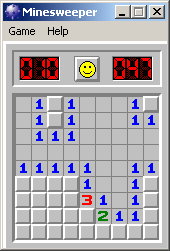
\includegraphics[scale=0.75]{\CURPATH/1.png}
\caption{Colored map}
\end{figure}

\subsubsection{MaxSMT or optimization problem}

Now let's have fun.
Out of pure whim, we may want to make as many countries colored as red as possible
\footnote{I took this idea from \url{https://www.cs.cmu.edu/~bryant/boolean/macgregor.html}}:

\begin{lstlisting}
s=Optimize()

...

s.maximize(Sum(*[If(country_color[i]==0, 1, 0) for i in range(countries_total)]))
\end{lstlisting}

\begin{figure}[H]
\centering
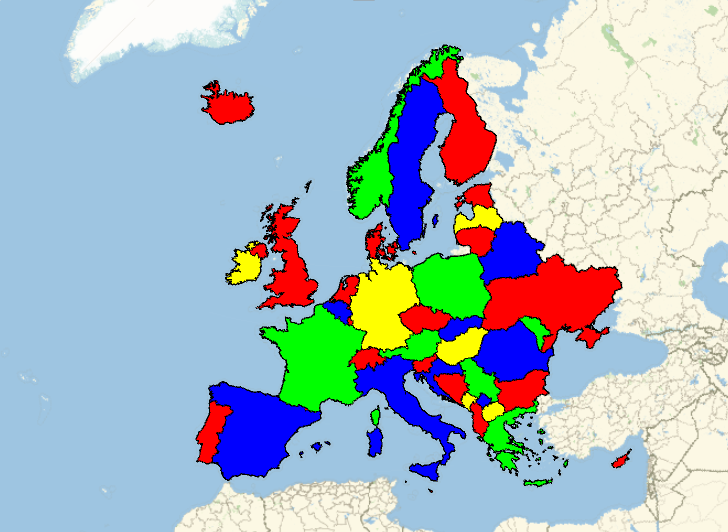
\includegraphics[scale=0.75]{\CURPATH/2_max_red.png}
\caption{The map}
\end{figure}

\lstinputlisting[caption=Statistics]{\CURPATH/2_max_red_stat.txt}

Or maybe we have a shortage of red paint?

\begin{lstlisting}
s.minimize(Sum(*[If(country_color[i]==0, 1, 0) for i in range(countries_total)]))
\end{lstlisting}

\begin{figure}[H]
\centering
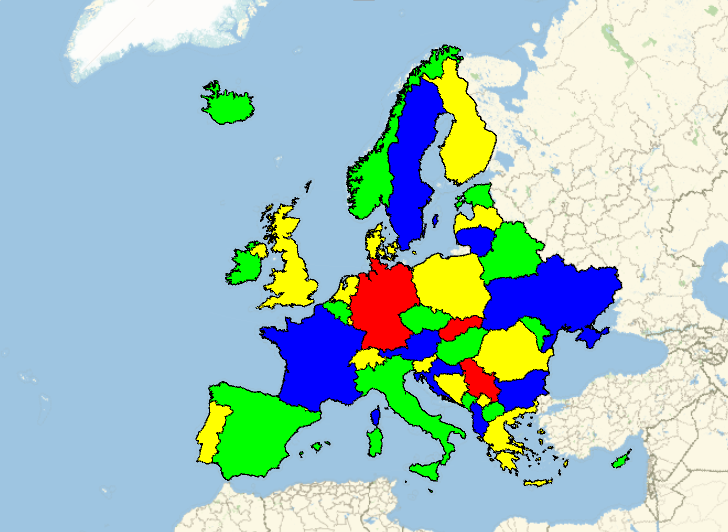
\includegraphics[scale=0.75]{\CURPATH/2_min_red.png}
\caption{The map}
\end{figure}

\lstinputlisting[caption=Statistics]{\CURPATH/2_min_red_stat.txt}

Two colors can be minimized/maximized simultaneously:

\begin{lstlisting}
...
s.minimize(Sum(*[If(Or(country_color[i]==0, country_color[i]==1), 1, 0) for i in range(countries_total)]))
...
\end{lstlisting}


\section{Using graph coloring in scheduling}

I've found this problem in the ``Discrete Structures, Logic and Computability'' book by James L. Hein:

\begin{figure}[H]
\centering
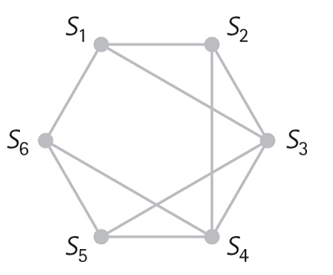
\includegraphics[scale=0.75]{color/fig144.png}
\caption{Graph}
\end{figure}

\begin{framed}
\begin{quotation}
Suppose some people form committees to do various tasks. The problem is to schedule the committee meetings in as few time slots as possible.
To simplify the discussion, we’ll represent each person with a number. For example, let S = {1, 2, 3, 4, 5, 6, 7} represent a set of seven people, and suppose they have formed six three-person committees as follows:

S1 = {1, 2, 3}, S2 = {2, 3, 4}, S3 = {3, 4, 5}, S4 = {4, 5, 6}, S5 = {5, 6, 7}, S6 = {1, 6, 7}.

We can model the problem with the graph pictured in Figure 1.4.4, where the committee names are the vertices and an edge connects two vertices if a person belongs to both committees represented by the vertices.
If each committee meets for one hour, what is the smallest number of hours needed for the committees to do their work?
From the graph, it follows that an edge between two committees means that they have at least one member in common.
Thus, they cannot meet at the same time. No edge between committees means that they can meet at the same time.
For example, committees S1 and S4 can meet the first hour. Then committees S2 and S5 can meet the second hour.
Finally, committees S3 and S6 can meet the third hour. Can you see why three hours is the smallest number of hours that the six committees can meet?
\end{quotation}
\end{framed}

And this is solution:

\lstinputlisting[style=custompy]{color/sched1.py}

The result:

\begin{lstlisting}
hour: 0 committees: [1, 4]
hour: 1 committees: [2, 5]
hour: 2 committees: [3, 6]
\end{lstlisting}

If you increase total number of hours to 4, the result is somewhat sparser:

\begin{lstlisting}
hour: 0 committees: [3]
hour: 1 committees: [1, 4]
hour: 2 committees: [2, 5]
hour: 3 committees: [6]
\end{lstlisting}


\section{Another example}

What if we want to divide our community/company/university by groups.
There are 16 persons and, which must be divided by 4 groups, 4 persons in each.
However, several persons hate each other, maybe, for personal reasons.
Can we group all them so the "haters" would be separated?

\lstinputlisting[style=custompy]{color/sched2.py}

The result:

\begin{lstlisting}
group 0, persons: [1, 2, 5, 8]
group 1, persons: [4, 7, 9, 12]
group 2, persons: [0, 3, 11, 13]
group 3, persons: [6, 10, 14, 15]
\end{lstlisting}


\subsection{Register allocation using graph coloring}

\renewcommand{\CURPATH}{color/reg_alloc}

This is an implementation of nuth-Morris-Pratt algorithm, it searches for a substring in a string
\footnote{Copypasted from \url{http://cprogramming.com/snippets/source-code/knuthmorrispratt-kmp-string-search-algorithm}}.

\lstinputlisting[style=customc]{\CURPATH/1.c}

... as you can see, I simplified it a bit, there are no more calls to malloc/free and T[] array is now global.

Then I compiled it using GCC 7.3 x64 and reworked assembly listing a little, now there are no registers, but rather vXX variables, each one is assigned only once,
in a \ac{SSA} manner. No variable assigned more than once. This is AT\&T syntax.

%FIXME:
%\lstinputlisting[style=customasm]{\CURPATH/KMP_template.s}
\lstinputlisting[basicstyle=\footnotesize]{\CURPATH/KMP_template.s}

Dangling "noodles" you see at right are "live ranges" of each vXX variable. "D" means "defined", "U" - "used" or "used and then defined again".
Whenever live range is started, we need to allocate variable (in a register or a local stack).
When it's ending, we do not need to keep it somewhere in storage (in a register or a local stack).

As you can see, the function has two parts: preparation and processing.
You can clearly see how live ranges are divided by two groups, except of first 4 variables, which are function arguments.

You see, there are 16 variables. But we want to use as small number of registers, as possible.
If several live ranges are present at some address or point of time, these variables cannot be allocated in the same register.

This is how we can assign a register to each live range using Z3 SMT-solver:

\lstinputlisting[style=custompy]{\CURPATH/solver.py}

What we've got for 12, 11 and 10 registers:

\lstinputlisting{\CURPATH/solver.txt}

It's not possible to assign 9 or less registers. 10 is a minimum.

Now all I do is replacing vXX variables to registers the SMT-solver offered:

\lstinputlisting[basicstyle=\footnotesize]{\CURPATH/KMP.s}

That works and it's almost the same as GCC does.

The problem of register allocation as a graph coloring problem: each live range is a vertex.
It a live range must coexist with another live range, put an edge between vertices, that means, vertices cannot share same color.
Color reflecting register number.

Almost all compilers (except simplest) do this in code generator. They use simpler algorithms, though, instead of such a heavy machinery as SAT/SMT solvers.

See also: \url{https://en.wikipedia.org/wiki/Register_allocation}, \url{https://en.wikipedia.org/wiki/Live_variable_analysis}.

Since graph coloring can have many solutions, you can probably hide some information
in "coloring": \url{https://yurichev.com/blog/lehmer/}.




\EN{\section{Knapsack problems}

\subsection{Popsicles}
\label{popsicles}

Found this problem at \url{http://artofproblemsolving.com/wiki/index.php?title=2017_AMC_12A_Problems/Problem_1}:

\begin{framed}
\begin{quotation}

Pablo buys popsicles for his friends. The store sells single popsicles for $\$$1 each, 3-popsicle boxes for $\$$2,
and 5-popsicle boxes for $\$$3. What is the greatest number of popsicles that Pablo can buy with $\$$8?

\end{quotation}
\end{framed}

This is optimization problem, and the solution using z3:

\lstinputlisting[style=custompy]{knapsack/1/popsicles.py}

The result:

\begin{lstlisting}
sat
[box3pop = 1,
 box5pop = 2,
 cost_total = 8,
 pop_total = 13,
 box1pop = 0]
\end{lstlisting}

\subsubsection{SMT-LIB 2.x}

\lstinputlisting[style=customsmt]{knapsack/1/popsicles.smt}



}
\RU{\section{Развлекательная математика и головоломки}

\subsection{Судоку}

Головоломка Судоку это решетка 9*9, некоторые ячейки заполнены значениями, некоторые пустые:

% copypasted from http://www.texample.net/tikz/examples/sudoku/
\newcounter{row}
\newcounter{col}

\newcommand\setrow[9]{
  \setcounter{col}{1}
  \foreach \n in {#1, #2, #3, #4, #5, #6, #7, #8, #9} {
    \edef\x{\value{col} - 0.5}
    \edef\y{9.5 - \value{row}}
    \node[anchor=center] at (\x, \y) {\n};
    \stepcounter{col}
  }
  \stepcounter{row}
}

\begin{center}
\begin{tikzpicture}[scale=.7]
  \begin{scope}
    \draw (0, 0) grid (9, 9);
    \draw[very thick, scale=3] (0, 0) grid (3, 3);

    \setcounter{row}{1}
    \setrow { }{ }{5}  {3}{ }{ }  { }{ }{ }
    \setrow {8}{ }{ }  { }{ }{ }  { }{2}{ }
    \setrow { }{7}{ }  { }{1}{ }  {5}{ }{ }

    \setrow {4}{ }{ }  { }{ }{5}  {3}{ }{ }
    \setrow { }{1}{ }  { }{7}{ }  { }{ }{6}
    \setrow { }{ }{3}  {2}{ }{ }  { }{8}{ }

    \setrow { }{6}{ }  {5}{ }{ }  { }{ }{9}
    \setrow { }{ }{4}  { }{ }{ }  { }{3}{ }
    \setrow { }{ }{ }  { }{ }{9}  {7}{ }{ }

    \node[anchor=center] at (4.5, -0.5) {Нерешенная Судоку};
  \end{scope}
\end{tikzpicture}
\end{center}

Числа в каждом ряду должны быть уникальными, т.е., каждый ряд должен содержать 9 чисел в пределах 1..9 без повторений.
Та же история и для каждого столбца и каждого квадрата 3*3.

Головоломка представляет собой хороший кандидат, на котором можно попробовать \ac{SMT}-солвер, потому что это,
в общем-то, просто нерешенная система уравнений.

\input{puzzles/sudoku/1/main_RU}
%\input{puzzles/sudoku/GT/main_RU}
%\input{puzzles/sudoku/killer/main_RU}
\input{puzzles/sudoku/KLEE/main_RU}
\input{puzzles/sudoku/SAT/main_RU}


\subsection{Головоломка зебры (\ac{AKA} Загадка Эйнштейна)}

\input{puzzles/zebra/SMT/main_RU}
\input{puzzles/zebra/KLEE/main_RU}
\input{puzzles/zebra/SAT/main_RU}


\subsection{Решение головоломки ``трубы'' используя Z3 SMT-солвер}

\renewcommand{\CURPATH}{puzzles/pipe}

Головоломка ``трубы'' это популярная головоломка (просто погуглите ``pipe puzzle'' и посмотрите на картинки).

Вот как выглядит головоломка в разобранном виде:

\begin{figure}[H]
\label{fig:pipe_shuffled}
\centering
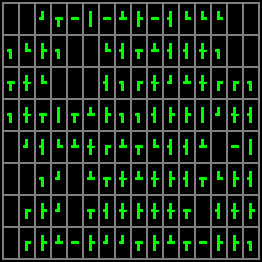
\includegraphics[scale=0.75]{\CURPATH/shuffled.png}
\caption{Разобранная головоломка}
\end{figure}

\dots и собранная:

\begin{figure}[H]
\label{fig:pipe_solved}
\centering
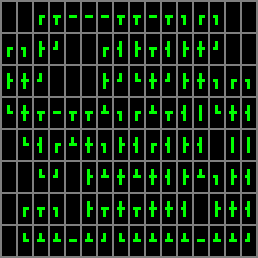
\includegraphics[scale=0.75]{\CURPATH/solved.png}
\caption{Собранная головоломка}
\end{figure}

Попробуем найти способ собрать её.

\subsubsection{Создание}

В начале, нужно её создать.
Вот простая идея.
Возьем массив ячеек 8*16.
Каждая ячейка может содержать какой-то тип блока.
Между ячейками есть стыки:

\input{\CURPATH/pipe_gen.tex}

Синие линии это горизонтальные стыки, красные линии это вертикальные стыки.
Мы просто случайно выставляем каждый стык в 0/false (отсутствует) или 1/true (присутствует).

После этого, теперь легко найти тип каждой ячейки.
А это:

\newcommand{\HeaderColor}{\cellcolor{blue!25}}
\begin{center}
\begin{longtable}{ | l | l | l | l | }
\hline
\HeaderColor стыки & \HeaderColor наше внутреннее название & \HeaderColor угол & \HeaderColor символ \\
\hline
0	&type 0		&	0$^{\circ}$	& (пробел)	\\
2	&type 2a	&	0$^{\circ}$	& \pmboxdrawuni{2503} \\ % ┃
2	&type 2a	&	90$^{\circ}$	& \pmboxdrawuni{2501} \\ % ━
2	&type 2b	&	0$^{\circ}$	& \pmboxdrawuni{250F} \\ % ┏
2	&type 2b	&	90$^{\circ}$	& \pmboxdrawuni{2513} \\ % ┓
2	&type 2b	&	180$^{\circ}$	& \pmboxdrawuni{251B} \\ % ┛
2	&type 2b	&	270$^{\circ}$	& \pmboxdrawuni{2517} \\ % ┗
3	&type 3		&	0$^{\circ}$	& \pmboxdrawuni{2523} \\ % ┣
3 	&type 3		&	90$^{\circ}$	& \pmboxdrawuni{2533} \\ % ┳
3	&type 3		&	180$^{\circ}$	& \pmboxdrawuni{252B} \\ % ┫
3	&type 3		&	270$^{\circ}$	& \pmboxdrawuni{253B} \\ % ┻
4	&type 4		&	0$^{\circ}$	& \pmboxdrawuni{254B} \\ % ╋
\hline
\end{longtable}
\end{center}

\textit{Висящие} стыки могут присутствовать на первой стадии (т.е., ячейки только с одним стыком), но они удалются
рекурсивно, и эти ячейки преобразуются в пустые ячейки.
Так что, в самом конце, все ячейки имеют минимум 2 стыка, и вся эта сантехническая система не имеет связей с внешним миром ---
я надеюсь, из-за этого станет немного проще.

Исходник генератора на Си здесь: \url{.../pipe/generator}.
Все вертикальные стыки хранятся в глобальном массиве \textit{hjoints[]} и вертикальные в \textit{vjoints[]}.

Программа на Си генерирует ANSI-раскрашенный вывод, как это было показано выше
(\ref{fig:pipe_shuffled}, \ref{fig:pipe_solved}) плюс массив типов для каждой ячейки, но без информации об углах:

\begin{lstlisting}[label=init_cells]
[
["0", "0", "2b", "3", "2a", "2a", "2a", "3", "3", "2a", "3", "2b", "2b", "2b", "0", "0"],
["2b", "2b", "3", "2b", "0", "0", "2b", "3", "3", "3", "3", "3", "4", "2b", "0", "0"],
["3", "4", "2b", "0", "0", "0", "3", "2b", "2b", "4", "2b", "3", "4", "2b", "2b", "2b"],
["2b", "4", "3", "2a", "3", "3", "3", "2b", "2b", "3", "3", "3", "2a", "2b", "4", "3"],
["0", "2b", "3", "2b", "3", "4", "2b", "3", "3", "2b", "3", "3", "3", "0", "2a", "2a"],
["0", "0", "2b", "2b", "0", "3", "3", "4", "3", "4", "3", "3", "3", "2b", "3", "3"],
["0", "2b", "3", "2b", "0", "3", "3", "4", "3", "4", "4", "3", "0", "3", "4", "3"],
["0", "2b", "3", "3", "2a", "3", "2b", "2b", "3", "3", "3", "3", "2a", "3", "3", "2b"],
]
\end{lstlisting}

\subsubsection{Решение}

Прежде всего, мы будем работать с массивом ячеек 8*16, где каждый элемент имеет 4 бита:
``T'' (top/верх),
``B'' (bottom/низ),
``L'' (left/лево),
``R'' (right/право).
Каждый бит представляет собой половину стыка.

\input{\CURPATH/pipe_solve.tex}

Теперь определяем массив для каждого из четырех полустыков + информация об угле:

\begin{lstlisting}
HEIGHT=8
WIDTH=16

# if T/B/R/L is Bool instead of Int, Z3 solver will work faster
T=[[Bool('cell_%d_%d_top' % (r, c)) for c in range(WIDTH)] for r in range(HEIGHT)]
B=[[Bool('cell_%d_%d_bottom' % (r, c)) for c in range(WIDTH)] for r in range(HEIGHT)]
R=[[Bool('cell_%d_%d_right' % (r, c)) for c in range(WIDTH)] for r in range(HEIGHT)]
L=[[Bool('cell_%d_%d_left' % (r, c)) for c in range(WIDTH)] for r in range(HEIGHT)]
A=[[Int('cell_%d_%d_angle' % (r, c)) for c in range(WIDTH)] for r in range(HEIGHT)]
\end{lstlisting}

Мы знаем, что если каждый из полустыков присутствует, ответный полустык также должен присутствовать, и наоборот. 
Определяем всё это используя эти констрайнты:

\begin{lstlisting}
# shorthand variables for True and False:
t=True
f=False

# "top" of each cell must be equal to "bottom" of the cell above
# "bottom" of each cell must be equal to "top" of the cell below
# "left" of each cell must be equal to "right" of the cell at left
# "right" of each cell must be equal to "left" of the cell at right
for r in range(HEIGHT):
    for c in range(WIDTH):
        if r!=0:
            s.add(T[r][c]==B[r-1][c])
        if r!=HEIGHT-1:
            s.add(B[r][c]==T[r+1][c])
        if c!=0:
            s.add(L[r][c]==R[r][c-1])
        if c!=WIDTH-1:
            s.add(R[r][c]==L[r][c+1])

# "left" of each cell of first column shouldn't have any connection
# so is "right" of each cell of the last column
for r in range(HEIGHT):
    s.add(L[r][0]==f)
    s.add(R[r][WIDTH-1]==f)

# "top" of each cell of the first row shouldn't have any connection
# so is "bottom" of each cell of the last row
for c in range(WIDTH):
    s.add(T[0][c]==f)
    s.add(B[HEIGHT-1][c]==f)
\end{lstlisting}

Теперь перебираем все ячейки в изначальном массиве (\ref{init_cells}).
Первые две ячейки здесь пустые. И третья имеет тип ``2b''.
Это ``\pmboxdrawuni{250F}'' % ┏
и его можно ориентировать четырьмя разными способами.
И если её угол это 0$^{\circ}$, верхний и правый полустыки присутствуют, остальные отсутствуют.
Если он имеет угол 90$^{\circ}$, он выглядит как 
``\pmboxdrawuni{2513}'', % ┓
и верхник и левый полустыки присутствуют, остальные отсутствуют.

На обычном русском языке: ``если ячейка этого типа имеет угол 0$^{\circ}$, вот эти полустыки должны присутствовать \textbf{ИЛИ}
если она имеет угол 90$^{\circ}$, эти полустыки должны присутствовать, \textbf{ИЛИ}, итд, итд.''

Точно также, мы определяем эти правила для всех типов и всех возможных углов:

\begin{lstlisting}
for r in range(HEIGHT):
    for c in range(WIDTH):
        ty=cells_type[r][c]

        if ty=="0":
            s.add(A[r][c]==f)
            s.add(T[r][c]==f, B[r][c]==f, L[r][c]==f, R[r][c]==f)

        if ty=="2a":
            s.add(Or(And(A[r][c]==0, L[r][c]==f, R[r][c]==f, T[r][c]==t, B[r][c]==t),   # §\pmboxdrawuni{2503}§
                    And(A[r][c]==90, L[r][c]==t, R[r][c]==t, T[r][c]==f, B[r][c]==f)))  # §\pmboxdrawuni{2501}§

        if ty=="2b":
            s.add(Or(And(A[r][c]==0, L[r][c]==f, R[r][c]==t, T[r][c]==f, B[r][c]==t),   # §\pmboxdrawuni{250F}§
                    And(A[r][c]==90, L[r][c]==t, R[r][c]==f, T[r][c]==f, B[r][c]==t),   # §\pmboxdrawuni{2513}§
                    And(A[r][c]==180, L[r][c]==t, R[r][c]==f, T[r][c]==t, B[r][c]==f),  # §\pmboxdrawuni{251B}§
                    And(A[r][c]==270, L[r][c]==f, R[r][c]==t, T[r][c]==t, B[r][c]==f))) # §\pmboxdrawuni{2517}§
	
        if ty=="3":
            s.add(Or(And(A[r][c]==0, L[r][c]==f, R[r][c]==t, T[r][c]==t, B[r][c]==t),   # §\pmboxdrawuni{2523}§
                    And(A[r][c]==90, L[r][c]==t, R[r][c]==t, T[r][c]==f, B[r][c]==t),   # §\pmboxdrawuni{2533}§
                    And(A[r][c]==180, L[r][c]==t, R[r][c]==f, T[r][c]==t, B[r][c]==t),  # §\pmboxdrawuni{252B}§
                    And(A[r][c]==270, L[r][c]==t, R[r][c]==t, T[r][c]==t, B[r][c]==f))) # §\pmboxdrawuni{253B}§

        if ty=="4":
            s.add(A[r][c]==0)
            s.add(T[r][c]==t, B[r][c]==t, L[r][c]==t, R[r][c]==t) # §\pmboxdrawuni{254B}§
\end{lstlisting}

Полный исходник здесь: \url{.../solver/solve_pipe_puzzle1.py}.

Получается такой результат (выводит угол для каждой ячейки и (псевдо)графическое представление):

\begin{figure}[H]
\centering
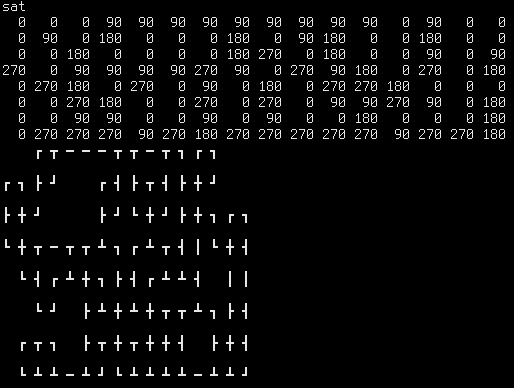
\includegraphics[scale=0.75]{\CURPATH/solver/solver.png}
\caption{Вывод скрипта солвера}
\end{figure}

Это работает $\approx 4$ секунды на моем старом и медленном Intel Atom N455 1.66GHz.
Быстро ли это? Не знаю, но снова вот что действительно круто, это то что мы понятия не имеем о какой-то математической
теории за всем этим, мы просто объявили ячейки, (полу-)стыки и определили отношения между ними.

Теперь следующий вопрос это, сколько здесь возможных решений?
Используя раннее описанный метод (\ref{SMTEnumerate}), я немного изменил скрипт солвера
\footnote{\url{.../solver/solve_pipe_puzzle2.py}} и солвер
сказал что возможно два решения.

Сравним их используя gvimdiff:

\begin{figure}[H]
\centering
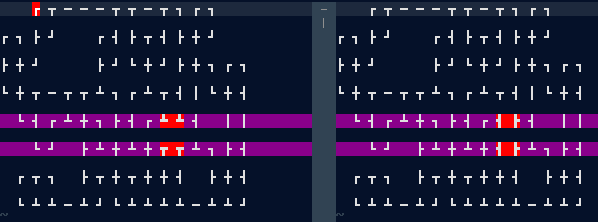
\includegraphics[scale=0.75]{\CURPATH/solver/diff.png}
\caption{Вывод gvimdiff (извините за мой красный курсор в левой части в левом верхнем углу)}
\end{figure}

4 ячейки в середине могут быть ориентированы по-разному.
Видимо, другие головоломки могут также выдавать разные результаты.

P.S.
\textit{Полу-стык} определен как булевый тип.
Но на самом деле, первая версия солвера была написана используя целочисленный тип для полу-стыков,
и 0 использовалось для False и 1 для True.
Я так сделал, потому что хотел более компактный исходный код, без использования длинных слов как ``False'' и ``True''.
И это работало, но медленнее. Вероятно, Z3 работает с булевыми типами быстрее? Лучше?
Так или иначе, я пишу это чтобы отметить, что, если нужно, целочисленный тип можно использовать вместо булевого.


\section{Развлекательная математика и головоломки}

\input{puzzles/sudoku/main_RU}
\input{puzzles/zebra/main_RU}
\input{puzzles/pipe/main_RU}
\input{puzzles/rubik2/failed_SMT/main_RU}
\input{puzzles/rubik2/SAT/main_RU}
\input{puzzles/rubik3/one_face_SMT/main_RU}
%\input{puzzles/numberlink/main_RU}
%\input{puzzles/two_parks_RU}
\input{puzzles/alphametics/main_RU}
%\input{puzzles/2015_AIME_II_Problems_12_RU}
%\input{puzzles/fred/main_RU}
%\input{puzzles/MC/main_RU}
%\input{puzzles/coin_flip/main_RU}
%\input{puzzles/Mock_AIME_2_2006-2007_Problem_8_RU}
%\input{puzzles/2012_AIME_I_Problems_1_RU}
%\input{puzzles/keypad_RU}


\section{Развлекательная математика и головоломки}

\input{puzzles/sudoku/main_RU}
\input{puzzles/zebra/main_RU}
\input{puzzles/pipe/main_RU}
\input{puzzles/rubik2/failed_SMT/main_RU}
\input{puzzles/rubik2/SAT/main_RU}
\input{puzzles/rubik3/one_face_SMT/main_RU}
%\input{puzzles/numberlink/main_RU}
%\input{puzzles/two_parks_RU}
\input{puzzles/alphametics/main_RU}
%\input{puzzles/2015_AIME_II_Problems_12_RU}
%\input{puzzles/fred/main_RU}
%\input{puzzles/MC/main_RU}
%\input{puzzles/coin_flip/main_RU}
%\input{puzzles/Mock_AIME_2_2006-2007_Problem_8_RU}
%\input{puzzles/2012_AIME_I_Problems_1_RU}
%\input{puzzles/keypad_RU}


\section{Развлекательная математика и головоломки}

\input{puzzles/sudoku/main_RU}
\input{puzzles/zebra/main_RU}
\input{puzzles/pipe/main_RU}
\input{puzzles/rubik2/failed_SMT/main_RU}
\input{puzzles/rubik2/SAT/main_RU}
\input{puzzles/rubik3/one_face_SMT/main_RU}
%\input{puzzles/numberlink/main_RU}
%\input{puzzles/two_parks_RU}
\input{puzzles/alphametics/main_RU}
%\input{puzzles/2015_AIME_II_Problems_12_RU}
%\input{puzzles/fred/main_RU}
%\input{puzzles/MC/main_RU}
%\input{puzzles/coin_flip/main_RU}
%\input{puzzles/Mock_AIME_2_2006-2007_Problem_8_RU}
%\input{puzzles/2012_AIME_I_Problems_1_RU}
%\input{puzzles/keypad_RU}


%\section{Развлекательная математика и головоломки}

\input{puzzles/sudoku/main_RU}
\input{puzzles/zebra/main_RU}
\input{puzzles/pipe/main_RU}
\input{puzzles/rubik2/failed_SMT/main_RU}
\input{puzzles/rubik2/SAT/main_RU}
\input{puzzles/rubik3/one_face_SMT/main_RU}
%\input{puzzles/numberlink/main_RU}
%\input{puzzles/two_parks_RU}
\input{puzzles/alphametics/main_RU}
%\input{puzzles/2015_AIME_II_Problems_12_RU}
%\input{puzzles/fred/main_RU}
%\input{puzzles/MC/main_RU}
%\input{puzzles/coin_flip/main_RU}
%\input{puzzles/Mock_AIME_2_2006-2007_Problem_8_RU}
%\input{puzzles/2012_AIME_I_Problems_1_RU}
%\input{puzzles/keypad_RU}


%\input{puzzles/two_parks_RU}
\subsection{Альфаметика}

Согласно Дональду Кнуту, термин ``Альфаметика'' был придуман Дж. Эйч. Аш. Хантером.
Это головоломка: какие десятичные цифры в пределах 0..9 нужно присвоить каждой букве, чтобы это уравнение было справедливо?

\begin{lstlisting}
  SEND
+ MORE
 -----
 MONEY
\end{lstlisting}

Для Z3 это легко:

\lstinputlisting{puzzles/alphametics/alpha.py}

Вывод:

\begin{lstlisting}
sat
[E, = 5,
 S, = 9,
 M, = 1,
 N, = 6,
 D, = 7,
 R, = 8,
 O, = 0,
 Y = 2]
\end{lstlisting}

Вот еще одна, из \ac{TAOCP} том IV (\url{http://www-cs-faculty.stanford.edu/~uno/fasc2b.ps.gz}):

\lstinputlisting{puzzles/alphametics/alpha2.py}

\begin{lstlisting}
sat
[L, = 6,
 S, = 7,
 N, = 2,
 T, = 1,
 I, = 5,
 V = 3,
 A, = 8,
 R, = 9,
 O, = 4,
 TRIO = 1954,
 SONATA, = 742818,
 VIOLA, = 35468,
 VIOLIN, = 354652]
\end{lstlisting}

% TODO URL
Эту головоломку я нашел в примерах pySMT:

\lstinputlisting{puzzles/alphametics/alpha3.py}

\begin{lstlisting}
sat
[D = 5, R = 4, O = 3, E = 8, L = 6, W = 7, H = 2]
\end{lstlisting}

%%% 

Это упражнение Q209 из
[Companion to the Papers of Donald Knuth]\footnote{\url{http://www-cs-faculty.stanford.edu/~knuth/cp.html}}.

\begin{lstlisting}
 KNIFE
  FORK
 SPOON
  SOUP
------
SUPPER
\end{lstlisting}

В целях упрощения, я добавил ф-цию (list\_to\_expr()):

\lstinputlisting{puzzles/alphametics/alpha4.py}

\begin{lstlisting}
sat
[K = 7,
 N = 4,
 R = 9,
 I = 1,
 E = 6,
 S = 0,
 O = 3,
 F = 5,
 U = 8,
 P = 2,
 SUPPER = 82269,
 SOUP = 382,
 SPOON = 2334,
 FORK = 5397,
 KNIFE = 74156]
\end{lstlisting}

S это 0, так что значение SUPPER начинается с (убранного) нуля. Скажем так, нам это не нравится.
Добавим это, чтобы это исправить:

\begin{lstlisting}
s.add(S!=0)
\end{lstlisting}

\begin{lstlisting}
sat
[K = 8,
 N = 4,
 R = 3,
 I = 7,
 E = 6,
 S = 1,
 O = 9,
 F = 2,
 U = 0,
 P = 5,
 SUPPER = 105563,
 SOUP = 1905,
 SPOON = 15994,
 FORK = 2938,
 KNIFE = 84726]
\end{lstlisting}

\paragraph{Создание своей собственной головоломки}

Вот проблема: есть только 10 букв, но как их выбрать из числа слов?
Мы можем использовать Z3 для этого:

\lstinputlisting{puzzles/alphametics/gen.py}

Это первая сгенерированная головоломка:

\begin{lstlisting}
sat
EGGS
JELLY
LUNCH
C 5
E 6
G 3
H 7
J 0
L 1
N 4
S 8
U 2
Y 9
\end{lstlisting}

Что если мы хотим, чтобы слово ``CAKE'' присутствовало в числе ``слагаемых''?

Добавим это:

\begin{lstlisting}
s.add(word_used[words.index('CAKE')])
\end{lstlisting}

\begin{lstlisting}
sat
CAKE
TEA
LUNCH
A 8
C 3
E 1
H 9
J 6
K 2
L 0
N 5
T 7
U 4
\end{lstlisting}

Добавим это:

\begin{lstlisting}
s.add(word_used[words.index('EGGS')])
\end{lstlisting}

Теперь оно может найти пару к EGGS:

\begin{lstlisting}
sat
EGGS
HONEY
LUNCH
C 6
E 7
G 9
H 4
L 5
N 8
O 2
S 3
U 0
Y 1
\end{lstlisting}

\paragraph{Файлы}

\url{https://github.com/DennisYurichev/...}




%\input{puzzles/2015_AIME_II_Problems_12_RU}
%\section{Развлекательная математика и головоломки}

\input{puzzles/sudoku/main_RU}
\input{puzzles/zebra/main_RU}
\input{puzzles/pipe/main_RU}
\input{puzzles/rubik2/failed_SMT/main_RU}
\input{puzzles/rubik2/SAT/main_RU}
\input{puzzles/rubik3/one_face_SMT/main_RU}
%\input{puzzles/numberlink/main_RU}
%\input{puzzles/two_parks_RU}
\input{puzzles/alphametics/main_RU}
%\input{puzzles/2015_AIME_II_Problems_12_RU}
%\input{puzzles/fred/main_RU}
%\input{puzzles/MC/main_RU}
%\input{puzzles/coin_flip/main_RU}
%\input{puzzles/Mock_AIME_2_2006-2007_Problem_8_RU}
%\input{puzzles/2012_AIME_I_Problems_1_RU}
%\input{puzzles/keypad_RU}


%\section{Развлекательная математика и головоломки}

\input{puzzles/sudoku/main_RU}
\input{puzzles/zebra/main_RU}
\input{puzzles/pipe/main_RU}
\input{puzzles/rubik2/failed_SMT/main_RU}
\input{puzzles/rubik2/SAT/main_RU}
\input{puzzles/rubik3/one_face_SMT/main_RU}
%\input{puzzles/numberlink/main_RU}
%\input{puzzles/two_parks_RU}
\input{puzzles/alphametics/main_RU}
%\input{puzzles/2015_AIME_II_Problems_12_RU}
%\input{puzzles/fred/main_RU}
%\input{puzzles/MC/main_RU}
%\input{puzzles/coin_flip/main_RU}
%\input{puzzles/Mock_AIME_2_2006-2007_Problem_8_RU}
%\input{puzzles/2012_AIME_I_Problems_1_RU}
%\input{puzzles/keypad_RU}


%\section{Развлекательная математика и головоломки}

\input{puzzles/sudoku/main_RU}
\input{puzzles/zebra/main_RU}
\input{puzzles/pipe/main_RU}
\input{puzzles/rubik2/failed_SMT/main_RU}
\input{puzzles/rubik2/SAT/main_RU}
\input{puzzles/rubik3/one_face_SMT/main_RU}
%\input{puzzles/numberlink/main_RU}
%\input{puzzles/two_parks_RU}
\input{puzzles/alphametics/main_RU}
%\input{puzzles/2015_AIME_II_Problems_12_RU}
%\input{puzzles/fred/main_RU}
%\input{puzzles/MC/main_RU}
%\input{puzzles/coin_flip/main_RU}
%\input{puzzles/Mock_AIME_2_2006-2007_Problem_8_RU}
%\input{puzzles/2012_AIME_I_Problems_1_RU}
%\input{puzzles/keypad_RU}


%\input{puzzles/Mock_AIME_2_2006-2007_Problem_8_RU}
%\input{puzzles/2012_AIME_I_Problems_1_RU}
%\input{puzzles/keypad_RU}

}


\EN{\chapter{Social Golfer Problem}

``Twenty golfers wish to play in foursomes for 5 days. Is it possible for each golfer to play no more than once with any other golfer?''
( \url{http://mathworld.wolfram.com/SocialGolferProblem.html} )

\subsection{Kirkman's Schoolgirl Problem (Z3Py)}

\begin{framed}
\begin{quotation}

Fifteen young ladies in a school walk out three abreast for seven days in succession: it is required to arrange them daily so that no two shall walk twice abreast.

\end{quotation}
\end{framed}

( \url{https://en.wikipedia.org/wiki/Kirkman%27s_schoolgirl_problem} )

This is naive and straightforward solution:

\lstinputlisting[style=custompy]{SGP/Z3/kirkman.py}

\begin{lstlisting}
sat
group for each person:
person:A B C D E F G H I J K L M N O
day=0: 2 2 3 1 0 0 3 4 0 1 1 3 4 4 2
day=1: 2 1 2 4 3 1 4 4 2 1 0 3 0 3 0
day=2: 4 3 1 0 4 0 4 2 2 1 2 3 3 0 1
day=3: 4 3 1 4 2 1 3 1 0 2 3 4 2 0 0
day=4: 3 0 0 1 1 2 4 3 4 3 2 2 4 0 1
day=5: 2 4 1 1 4 3 3 4 0 0 2 0 1 2 3
day=6: 0 2 4 2 4 0 1 3 2 1 4 3 0 1 3

persons grouped:
day=0: EFI  DJK  ABO  CGL  HMN
day=1: KMO  BFJ  ACI  ELN  DGH
day=2: DFN  CJO  HIK  BLM  AEG
day=3: INO  CFH  EJM  BGK  ADL
day=4: BCN  DEO  FKL  AHJ  GIM
day=5: IJL  CDM  AKN  FGO  BEH
day=6: AFM  GJN  BDI  HLO  CEK
\end{lstlisting}

It took $\approx 48$ seconds on my old Intel Xeon E3-1220 3.10GHz.

I've also tried to represent each number (group in which schoolgirl/golfer is) as a single bit:

\lstinputlisting[style=custompy]{SGP/Z3/kirkman2.py}

This is way faster, $\approx 1.5$ seconds on the same CPU.

Unfortunately, sample \ac{SGP} are out of reach. Yet?
\url{http://www.mathpuzzle.com/MAA/54-Golf%20Tournaments/mathgames_08_14_07.html}.

The files: \url{https://github.com/DennisYurichev/SAT_SMT_by_example/tree/master/SGP/Z3}.


\subsection{School teams scheduling (SAT)}

I've found this in the [Dennis E. Shasha -- "Puzzles for Programmers and Pros"] book:

\begin{framed}
\begin{quotation}
Scheduling Tradition

There are 12 school teams, unimaginatively named A, B, C, D, E, F, G, H, I, J, K, and L. They must play one another on 11 consecutive days on six fields. 
Every team must play every other team exactly once. Each team plays one game per day.

        Warm-Up
                Suppose there were four teams A, B, C, D and each team has to play every other in three days on two fields. How can you do it?

        Solution to Warm-Up

                We’ll represent the solution in two columns corresponding to the two playing fields. Thus, in the first day, A plays B on field 1 and C plays D on field 2.
                AB CD
                AC DB
                AD BC

Not only does the real problem involve 12 teams instead of merely four, but there are certain constraints due to traditional team rivalries: 
A must play B on day 1, G on day 3, and H on day 6. F must play I on day 2 and J on day 5.  K must play H on day 9 and E on day 11. 
L must play E on day 8 and B on day 9. H must play I on day 10 and L on day 11. There are no constraints on C or D because these are new teams.

        1. Can you form an 11-day schedule for these teams that satisfies the constraints?

It may seem difficult, but look again at the warm-up. Look in particular at the non-A columns. They are related to one another.
If you understand how, you can solve the harder problem.
\end{quotation}
\end{framed}

% TODO \ref{}
This is like Kirkman's Schoolgirl Problem I have solved using Z3 before, but this time I've rewritten it as a SAT problem.
Also, I added additional constraints relating to ``team rivalries''.

\lstinputlisting[style=custompy]{SGP/SAT/kirkman_SAT.py}

The solution:

\begin{lstlisting}
group for each person:
person: A B C D E F G H I J K L
day= 0: 4 4 1 3 5 0 2 0 5 3 2 1
day= 1: 5 0 3 3 2 4 1 2 4 1 0 5
day= 2: 4 5 1 0 1 2 4 5 3 3 2 0
day= 3: 3 5 4 1 1 4 2 2 0 5 3 0
day= 4: 3 0 4 5 0 2 5 3 4 2 1 1
day= 5: 3 5 4 5 3 0 0 4 1 2 1 2
day= 6: 5 3 5 4 1 0 1 4 3 2 2 0
day= 7: 5 2 0 1 3 1 2 4 5 4 0 3
day= 8: 4 2 5 4 1 1 3 0 3 5 0 2
day= 9: 4 2 2 1 5 4 0 3 3 5 1 0
day=10: 2 5 0 4 3 5 0 1 4 2 3 1

persons grouped:
day= 0: FH  CL  GK  DJ  AB  EI
day= 1: BK  GJ  EH  CD  FI  AL
day= 2: DL  CE  FK  IJ  AG  BH
day= 3: IL  DE  GH  AK  CF  BJ
day= 4: BE  KL  FJ  AH  CI  DG
day= 5: FG  IK  JL  AE  CH  BD
day= 6: FL  EG  JK  BI  DH  AC
day= 7: CK  DF  BG  EL  HJ  AI
day= 8: HK  EF  BL  GI  AD  CJ
day= 9: GL  DK  BC  HI  AF  EJ
day=10: CG  HL  AJ  EK  DI  BF
\end{lstlisting}

(``Person'' and ``team'' terms are interchangeable in my code.)

Thanks to 
parallel lingeling SAT solver\footnote{\url{http://fmv.jku.at/lingeling/}}
I've used this time, it takes couple of minutes on a decent 4-core CPU.

The source code: \url{https://github.com/DennisYurichev/SAT_SMT_by_example/tree/master/SGP/SAT}.



}
\RU{\section{Развлекательная математика и головоломки}

\subsection{Судоку}

Головоломка Судоку это решетка 9*9, некоторые ячейки заполнены значениями, некоторые пустые:

% copypasted from http://www.texample.net/tikz/examples/sudoku/
\newcounter{row}
\newcounter{col}

\newcommand\setrow[9]{
  \setcounter{col}{1}
  \foreach \n in {#1, #2, #3, #4, #5, #6, #7, #8, #9} {
    \edef\x{\value{col} - 0.5}
    \edef\y{9.5 - \value{row}}
    \node[anchor=center] at (\x, \y) {\n};
    \stepcounter{col}
  }
  \stepcounter{row}
}

\begin{center}
\begin{tikzpicture}[scale=.7]
  \begin{scope}
    \draw (0, 0) grid (9, 9);
    \draw[very thick, scale=3] (0, 0) grid (3, 3);

    \setcounter{row}{1}
    \setrow { }{ }{5}  {3}{ }{ }  { }{ }{ }
    \setrow {8}{ }{ }  { }{ }{ }  { }{2}{ }
    \setrow { }{7}{ }  { }{1}{ }  {5}{ }{ }

    \setrow {4}{ }{ }  { }{ }{5}  {3}{ }{ }
    \setrow { }{1}{ }  { }{7}{ }  { }{ }{6}
    \setrow { }{ }{3}  {2}{ }{ }  { }{8}{ }

    \setrow { }{6}{ }  {5}{ }{ }  { }{ }{9}
    \setrow { }{ }{4}  { }{ }{ }  { }{3}{ }
    \setrow { }{ }{ }  { }{ }{9}  {7}{ }{ }

    \node[anchor=center] at (4.5, -0.5) {Нерешенная Судоку};
  \end{scope}
\end{tikzpicture}
\end{center}

Числа в каждом ряду должны быть уникальными, т.е., каждый ряд должен содержать 9 чисел в пределах 1..9 без повторений.
Та же история и для каждого столбца и каждого квадрата 3*3.

Головоломка представляет собой хороший кандидат, на котором можно попробовать \ac{SMT}-солвер, потому что это,
в общем-то, просто нерешенная система уравнений.

\input{puzzles/sudoku/1/main_RU}
%\input{puzzles/sudoku/GT/main_RU}
%\input{puzzles/sudoku/killer/main_RU}
\input{puzzles/sudoku/KLEE/main_RU}
\input{puzzles/sudoku/SAT/main_RU}


\subsection{Головоломка зебры (\ac{AKA} Загадка Эйнштейна)}

\input{puzzles/zebra/SMT/main_RU}
\input{puzzles/zebra/KLEE/main_RU}
\input{puzzles/zebra/SAT/main_RU}


\subsection{Решение головоломки ``трубы'' используя Z3 SMT-солвер}

\renewcommand{\CURPATH}{puzzles/pipe}

Головоломка ``трубы'' это популярная головоломка (просто погуглите ``pipe puzzle'' и посмотрите на картинки).

Вот как выглядит головоломка в разобранном виде:

\begin{figure}[H]
\label{fig:pipe_shuffled}
\centering
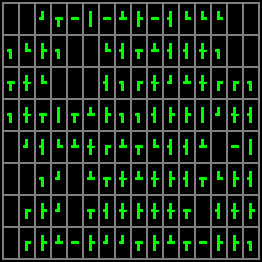
\includegraphics[scale=0.75]{\CURPATH/shuffled.png}
\caption{Разобранная головоломка}
\end{figure}

\dots и собранная:

\begin{figure}[H]
\label{fig:pipe_solved}
\centering
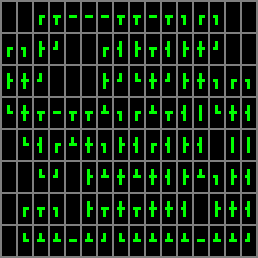
\includegraphics[scale=0.75]{\CURPATH/solved.png}
\caption{Собранная головоломка}
\end{figure}

Попробуем найти способ собрать её.

\subsubsection{Создание}

В начале, нужно её создать.
Вот простая идея.
Возьем массив ячеек 8*16.
Каждая ячейка может содержать какой-то тип блока.
Между ячейками есть стыки:

\input{\CURPATH/pipe_gen.tex}

Синие линии это горизонтальные стыки, красные линии это вертикальные стыки.
Мы просто случайно выставляем каждый стык в 0/false (отсутствует) или 1/true (присутствует).

После этого, теперь легко найти тип каждой ячейки.
А это:

\newcommand{\HeaderColor}{\cellcolor{blue!25}}
\begin{center}
\begin{longtable}{ | l | l | l | l | }
\hline
\HeaderColor стыки & \HeaderColor наше внутреннее название & \HeaderColor угол & \HeaderColor символ \\
\hline
0	&type 0		&	0$^{\circ}$	& (пробел)	\\
2	&type 2a	&	0$^{\circ}$	& \pmboxdrawuni{2503} \\ % ┃
2	&type 2a	&	90$^{\circ}$	& \pmboxdrawuni{2501} \\ % ━
2	&type 2b	&	0$^{\circ}$	& \pmboxdrawuni{250F} \\ % ┏
2	&type 2b	&	90$^{\circ}$	& \pmboxdrawuni{2513} \\ % ┓
2	&type 2b	&	180$^{\circ}$	& \pmboxdrawuni{251B} \\ % ┛
2	&type 2b	&	270$^{\circ}$	& \pmboxdrawuni{2517} \\ % ┗
3	&type 3		&	0$^{\circ}$	& \pmboxdrawuni{2523} \\ % ┣
3 	&type 3		&	90$^{\circ}$	& \pmboxdrawuni{2533} \\ % ┳
3	&type 3		&	180$^{\circ}$	& \pmboxdrawuni{252B} \\ % ┫
3	&type 3		&	270$^{\circ}$	& \pmboxdrawuni{253B} \\ % ┻
4	&type 4		&	0$^{\circ}$	& \pmboxdrawuni{254B} \\ % ╋
\hline
\end{longtable}
\end{center}

\textit{Висящие} стыки могут присутствовать на первой стадии (т.е., ячейки только с одним стыком), но они удалются
рекурсивно, и эти ячейки преобразуются в пустые ячейки.
Так что, в самом конце, все ячейки имеют минимум 2 стыка, и вся эта сантехническая система не имеет связей с внешним миром ---
я надеюсь, из-за этого станет немного проще.

Исходник генератора на Си здесь: \url{.../pipe/generator}.
Все вертикальные стыки хранятся в глобальном массиве \textit{hjoints[]} и вертикальные в \textit{vjoints[]}.

Программа на Си генерирует ANSI-раскрашенный вывод, как это было показано выше
(\ref{fig:pipe_shuffled}, \ref{fig:pipe_solved}) плюс массив типов для каждой ячейки, но без информации об углах:

\begin{lstlisting}[label=init_cells]
[
["0", "0", "2b", "3", "2a", "2a", "2a", "3", "3", "2a", "3", "2b", "2b", "2b", "0", "0"],
["2b", "2b", "3", "2b", "0", "0", "2b", "3", "3", "3", "3", "3", "4", "2b", "0", "0"],
["3", "4", "2b", "0", "0", "0", "3", "2b", "2b", "4", "2b", "3", "4", "2b", "2b", "2b"],
["2b", "4", "3", "2a", "3", "3", "3", "2b", "2b", "3", "3", "3", "2a", "2b", "4", "3"],
["0", "2b", "3", "2b", "3", "4", "2b", "3", "3", "2b", "3", "3", "3", "0", "2a", "2a"],
["0", "0", "2b", "2b", "0", "3", "3", "4", "3", "4", "3", "3", "3", "2b", "3", "3"],
["0", "2b", "3", "2b", "0", "3", "3", "4", "3", "4", "4", "3", "0", "3", "4", "3"],
["0", "2b", "3", "3", "2a", "3", "2b", "2b", "3", "3", "3", "3", "2a", "3", "3", "2b"],
]
\end{lstlisting}

\subsubsection{Решение}

Прежде всего, мы будем работать с массивом ячеек 8*16, где каждый элемент имеет 4 бита:
``T'' (top/верх),
``B'' (bottom/низ),
``L'' (left/лево),
``R'' (right/право).
Каждый бит представляет собой половину стыка.

\input{\CURPATH/pipe_solve.tex}

Теперь определяем массив для каждого из четырех полустыков + информация об угле:

\begin{lstlisting}
HEIGHT=8
WIDTH=16

# if T/B/R/L is Bool instead of Int, Z3 solver will work faster
T=[[Bool('cell_%d_%d_top' % (r, c)) for c in range(WIDTH)] for r in range(HEIGHT)]
B=[[Bool('cell_%d_%d_bottom' % (r, c)) for c in range(WIDTH)] for r in range(HEIGHT)]
R=[[Bool('cell_%d_%d_right' % (r, c)) for c in range(WIDTH)] for r in range(HEIGHT)]
L=[[Bool('cell_%d_%d_left' % (r, c)) for c in range(WIDTH)] for r in range(HEIGHT)]
A=[[Int('cell_%d_%d_angle' % (r, c)) for c in range(WIDTH)] for r in range(HEIGHT)]
\end{lstlisting}

Мы знаем, что если каждый из полустыков присутствует, ответный полустык также должен присутствовать, и наоборот. 
Определяем всё это используя эти констрайнты:

\begin{lstlisting}
# shorthand variables for True and False:
t=True
f=False

# "top" of each cell must be equal to "bottom" of the cell above
# "bottom" of each cell must be equal to "top" of the cell below
# "left" of each cell must be equal to "right" of the cell at left
# "right" of each cell must be equal to "left" of the cell at right
for r in range(HEIGHT):
    for c in range(WIDTH):
        if r!=0:
            s.add(T[r][c]==B[r-1][c])
        if r!=HEIGHT-1:
            s.add(B[r][c]==T[r+1][c])
        if c!=0:
            s.add(L[r][c]==R[r][c-1])
        if c!=WIDTH-1:
            s.add(R[r][c]==L[r][c+1])

# "left" of each cell of first column shouldn't have any connection
# so is "right" of each cell of the last column
for r in range(HEIGHT):
    s.add(L[r][0]==f)
    s.add(R[r][WIDTH-1]==f)

# "top" of each cell of the first row shouldn't have any connection
# so is "bottom" of each cell of the last row
for c in range(WIDTH):
    s.add(T[0][c]==f)
    s.add(B[HEIGHT-1][c]==f)
\end{lstlisting}

Теперь перебираем все ячейки в изначальном массиве (\ref{init_cells}).
Первые две ячейки здесь пустые. И третья имеет тип ``2b''.
Это ``\pmboxdrawuni{250F}'' % ┏
и его можно ориентировать четырьмя разными способами.
И если её угол это 0$^{\circ}$, верхний и правый полустыки присутствуют, остальные отсутствуют.
Если он имеет угол 90$^{\circ}$, он выглядит как 
``\pmboxdrawuni{2513}'', % ┓
и верхник и левый полустыки присутствуют, остальные отсутствуют.

На обычном русском языке: ``если ячейка этого типа имеет угол 0$^{\circ}$, вот эти полустыки должны присутствовать \textbf{ИЛИ}
если она имеет угол 90$^{\circ}$, эти полустыки должны присутствовать, \textbf{ИЛИ}, итд, итд.''

Точно также, мы определяем эти правила для всех типов и всех возможных углов:

\begin{lstlisting}
for r in range(HEIGHT):
    for c in range(WIDTH):
        ty=cells_type[r][c]

        if ty=="0":
            s.add(A[r][c]==f)
            s.add(T[r][c]==f, B[r][c]==f, L[r][c]==f, R[r][c]==f)

        if ty=="2a":
            s.add(Or(And(A[r][c]==0, L[r][c]==f, R[r][c]==f, T[r][c]==t, B[r][c]==t),   # §\pmboxdrawuni{2503}§
                    And(A[r][c]==90, L[r][c]==t, R[r][c]==t, T[r][c]==f, B[r][c]==f)))  # §\pmboxdrawuni{2501}§

        if ty=="2b":
            s.add(Or(And(A[r][c]==0, L[r][c]==f, R[r][c]==t, T[r][c]==f, B[r][c]==t),   # §\pmboxdrawuni{250F}§
                    And(A[r][c]==90, L[r][c]==t, R[r][c]==f, T[r][c]==f, B[r][c]==t),   # §\pmboxdrawuni{2513}§
                    And(A[r][c]==180, L[r][c]==t, R[r][c]==f, T[r][c]==t, B[r][c]==f),  # §\pmboxdrawuni{251B}§
                    And(A[r][c]==270, L[r][c]==f, R[r][c]==t, T[r][c]==t, B[r][c]==f))) # §\pmboxdrawuni{2517}§
	
        if ty=="3":
            s.add(Or(And(A[r][c]==0, L[r][c]==f, R[r][c]==t, T[r][c]==t, B[r][c]==t),   # §\pmboxdrawuni{2523}§
                    And(A[r][c]==90, L[r][c]==t, R[r][c]==t, T[r][c]==f, B[r][c]==t),   # §\pmboxdrawuni{2533}§
                    And(A[r][c]==180, L[r][c]==t, R[r][c]==f, T[r][c]==t, B[r][c]==t),  # §\pmboxdrawuni{252B}§
                    And(A[r][c]==270, L[r][c]==t, R[r][c]==t, T[r][c]==t, B[r][c]==f))) # §\pmboxdrawuni{253B}§

        if ty=="4":
            s.add(A[r][c]==0)
            s.add(T[r][c]==t, B[r][c]==t, L[r][c]==t, R[r][c]==t) # §\pmboxdrawuni{254B}§
\end{lstlisting}

Полный исходник здесь: \url{.../solver/solve_pipe_puzzle1.py}.

Получается такой результат (выводит угол для каждой ячейки и (псевдо)графическое представление):

\begin{figure}[H]
\centering
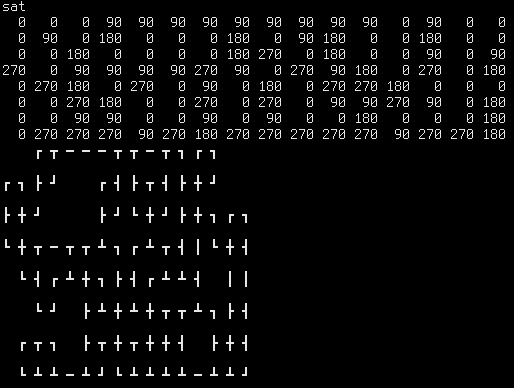
\includegraphics[scale=0.75]{\CURPATH/solver/solver.png}
\caption{Вывод скрипта солвера}
\end{figure}

Это работает $\approx 4$ секунды на моем старом и медленном Intel Atom N455 1.66GHz.
Быстро ли это? Не знаю, но снова вот что действительно круто, это то что мы понятия не имеем о какой-то математической
теории за всем этим, мы просто объявили ячейки, (полу-)стыки и определили отношения между ними.

Теперь следующий вопрос это, сколько здесь возможных решений?
Используя раннее описанный метод (\ref{SMTEnumerate}), я немного изменил скрипт солвера
\footnote{\url{.../solver/solve_pipe_puzzle2.py}} и солвер
сказал что возможно два решения.

Сравним их используя gvimdiff:

\begin{figure}[H]
\centering
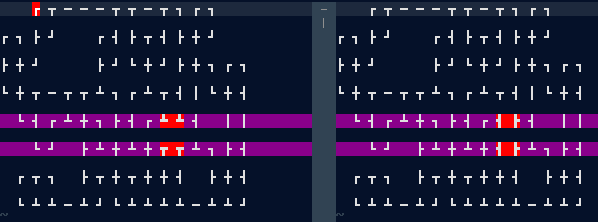
\includegraphics[scale=0.75]{\CURPATH/solver/diff.png}
\caption{Вывод gvimdiff (извините за мой красный курсор в левой части в левом верхнем углу)}
\end{figure}

4 ячейки в середине могут быть ориентированы по-разному.
Видимо, другие головоломки могут также выдавать разные результаты.

P.S.
\textit{Полу-стык} определен как булевый тип.
Но на самом деле, первая версия солвера была написана используя целочисленный тип для полу-стыков,
и 0 использовалось для False и 1 для True.
Я так сделал, потому что хотел более компактный исходный код, без использования длинных слов как ``False'' и ``True''.
И это работало, но медленнее. Вероятно, Z3 работает с булевыми типами быстрее? Лучше?
Так или иначе, я пишу это чтобы отметить, что, если нужно, целочисленный тип можно использовать вместо булевого.


\section{Развлекательная математика и головоломки}

\input{puzzles/sudoku/main_RU}
\input{puzzles/zebra/main_RU}
\input{puzzles/pipe/main_RU}
\input{puzzles/rubik2/failed_SMT/main_RU}
\input{puzzles/rubik2/SAT/main_RU}
\input{puzzles/rubik3/one_face_SMT/main_RU}
%\input{puzzles/numberlink/main_RU}
%\input{puzzles/two_parks_RU}
\input{puzzles/alphametics/main_RU}
%\input{puzzles/2015_AIME_II_Problems_12_RU}
%\input{puzzles/fred/main_RU}
%\input{puzzles/MC/main_RU}
%\input{puzzles/coin_flip/main_RU}
%\input{puzzles/Mock_AIME_2_2006-2007_Problem_8_RU}
%\input{puzzles/2012_AIME_I_Problems_1_RU}
%\input{puzzles/keypad_RU}


\section{Развлекательная математика и головоломки}

\input{puzzles/sudoku/main_RU}
\input{puzzles/zebra/main_RU}
\input{puzzles/pipe/main_RU}
\input{puzzles/rubik2/failed_SMT/main_RU}
\input{puzzles/rubik2/SAT/main_RU}
\input{puzzles/rubik3/one_face_SMT/main_RU}
%\input{puzzles/numberlink/main_RU}
%\input{puzzles/two_parks_RU}
\input{puzzles/alphametics/main_RU}
%\input{puzzles/2015_AIME_II_Problems_12_RU}
%\input{puzzles/fred/main_RU}
%\input{puzzles/MC/main_RU}
%\input{puzzles/coin_flip/main_RU}
%\input{puzzles/Mock_AIME_2_2006-2007_Problem_8_RU}
%\input{puzzles/2012_AIME_I_Problems_1_RU}
%\input{puzzles/keypad_RU}


\section{Развлекательная математика и головоломки}

\input{puzzles/sudoku/main_RU}
\input{puzzles/zebra/main_RU}
\input{puzzles/pipe/main_RU}
\input{puzzles/rubik2/failed_SMT/main_RU}
\input{puzzles/rubik2/SAT/main_RU}
\input{puzzles/rubik3/one_face_SMT/main_RU}
%\input{puzzles/numberlink/main_RU}
%\input{puzzles/two_parks_RU}
\input{puzzles/alphametics/main_RU}
%\input{puzzles/2015_AIME_II_Problems_12_RU}
%\input{puzzles/fred/main_RU}
%\input{puzzles/MC/main_RU}
%\input{puzzles/coin_flip/main_RU}
%\input{puzzles/Mock_AIME_2_2006-2007_Problem_8_RU}
%\input{puzzles/2012_AIME_I_Problems_1_RU}
%\input{puzzles/keypad_RU}


%\section{Развлекательная математика и головоломки}

\input{puzzles/sudoku/main_RU}
\input{puzzles/zebra/main_RU}
\input{puzzles/pipe/main_RU}
\input{puzzles/rubik2/failed_SMT/main_RU}
\input{puzzles/rubik2/SAT/main_RU}
\input{puzzles/rubik3/one_face_SMT/main_RU}
%\input{puzzles/numberlink/main_RU}
%\input{puzzles/two_parks_RU}
\input{puzzles/alphametics/main_RU}
%\input{puzzles/2015_AIME_II_Problems_12_RU}
%\input{puzzles/fred/main_RU}
%\input{puzzles/MC/main_RU}
%\input{puzzles/coin_flip/main_RU}
%\input{puzzles/Mock_AIME_2_2006-2007_Problem_8_RU}
%\input{puzzles/2012_AIME_I_Problems_1_RU}
%\input{puzzles/keypad_RU}


%\input{puzzles/two_parks_RU}
\subsection{Альфаметика}

Согласно Дональду Кнуту, термин ``Альфаметика'' был придуман Дж. Эйч. Аш. Хантером.
Это головоломка: какие десятичные цифры в пределах 0..9 нужно присвоить каждой букве, чтобы это уравнение было справедливо?

\begin{lstlisting}
  SEND
+ MORE
 -----
 MONEY
\end{lstlisting}

Для Z3 это легко:

\lstinputlisting{puzzles/alphametics/alpha.py}

Вывод:

\begin{lstlisting}
sat
[E, = 5,
 S, = 9,
 M, = 1,
 N, = 6,
 D, = 7,
 R, = 8,
 O, = 0,
 Y = 2]
\end{lstlisting}

Вот еще одна, из \ac{TAOCP} том IV (\url{http://www-cs-faculty.stanford.edu/~uno/fasc2b.ps.gz}):

\lstinputlisting{puzzles/alphametics/alpha2.py}

\begin{lstlisting}
sat
[L, = 6,
 S, = 7,
 N, = 2,
 T, = 1,
 I, = 5,
 V = 3,
 A, = 8,
 R, = 9,
 O, = 4,
 TRIO = 1954,
 SONATA, = 742818,
 VIOLA, = 35468,
 VIOLIN, = 354652]
\end{lstlisting}

% TODO URL
Эту головоломку я нашел в примерах pySMT:

\lstinputlisting{puzzles/alphametics/alpha3.py}

\begin{lstlisting}
sat
[D = 5, R = 4, O = 3, E = 8, L = 6, W = 7, H = 2]
\end{lstlisting}

%%% 

Это упражнение Q209 из
[Companion to the Papers of Donald Knuth]\footnote{\url{http://www-cs-faculty.stanford.edu/~knuth/cp.html}}.

\begin{lstlisting}
 KNIFE
  FORK
 SPOON
  SOUP
------
SUPPER
\end{lstlisting}

В целях упрощения, я добавил ф-цию (list\_to\_expr()):

\lstinputlisting{puzzles/alphametics/alpha4.py}

\begin{lstlisting}
sat
[K = 7,
 N = 4,
 R = 9,
 I = 1,
 E = 6,
 S = 0,
 O = 3,
 F = 5,
 U = 8,
 P = 2,
 SUPPER = 82269,
 SOUP = 382,
 SPOON = 2334,
 FORK = 5397,
 KNIFE = 74156]
\end{lstlisting}

S это 0, так что значение SUPPER начинается с (убранного) нуля. Скажем так, нам это не нравится.
Добавим это, чтобы это исправить:

\begin{lstlisting}
s.add(S!=0)
\end{lstlisting}

\begin{lstlisting}
sat
[K = 8,
 N = 4,
 R = 3,
 I = 7,
 E = 6,
 S = 1,
 O = 9,
 F = 2,
 U = 0,
 P = 5,
 SUPPER = 105563,
 SOUP = 1905,
 SPOON = 15994,
 FORK = 2938,
 KNIFE = 84726]
\end{lstlisting}

\paragraph{Создание своей собственной головоломки}

Вот проблема: есть только 10 букв, но как их выбрать из числа слов?
Мы можем использовать Z3 для этого:

\lstinputlisting{puzzles/alphametics/gen.py}

Это первая сгенерированная головоломка:

\begin{lstlisting}
sat
EGGS
JELLY
LUNCH
C 5
E 6
G 3
H 7
J 0
L 1
N 4
S 8
U 2
Y 9
\end{lstlisting}

Что если мы хотим, чтобы слово ``CAKE'' присутствовало в числе ``слагаемых''?

Добавим это:

\begin{lstlisting}
s.add(word_used[words.index('CAKE')])
\end{lstlisting}

\begin{lstlisting}
sat
CAKE
TEA
LUNCH
A 8
C 3
E 1
H 9
J 6
K 2
L 0
N 5
T 7
U 4
\end{lstlisting}

Добавим это:

\begin{lstlisting}
s.add(word_used[words.index('EGGS')])
\end{lstlisting}

Теперь оно может найти пару к EGGS:

\begin{lstlisting}
sat
EGGS
HONEY
LUNCH
C 6
E 7
G 9
H 4
L 5
N 8
O 2
S 3
U 0
Y 1
\end{lstlisting}

\paragraph{Файлы}

\url{https://github.com/DennisYurichev/...}




%\input{puzzles/2015_AIME_II_Problems_12_RU}
%\section{Развлекательная математика и головоломки}

\input{puzzles/sudoku/main_RU}
\input{puzzles/zebra/main_RU}
\input{puzzles/pipe/main_RU}
\input{puzzles/rubik2/failed_SMT/main_RU}
\input{puzzles/rubik2/SAT/main_RU}
\input{puzzles/rubik3/one_face_SMT/main_RU}
%\input{puzzles/numberlink/main_RU}
%\input{puzzles/two_parks_RU}
\input{puzzles/alphametics/main_RU}
%\input{puzzles/2015_AIME_II_Problems_12_RU}
%\input{puzzles/fred/main_RU}
%\input{puzzles/MC/main_RU}
%\input{puzzles/coin_flip/main_RU}
%\input{puzzles/Mock_AIME_2_2006-2007_Problem_8_RU}
%\input{puzzles/2012_AIME_I_Problems_1_RU}
%\input{puzzles/keypad_RU}


%\section{Развлекательная математика и головоломки}

\input{puzzles/sudoku/main_RU}
\input{puzzles/zebra/main_RU}
\input{puzzles/pipe/main_RU}
\input{puzzles/rubik2/failed_SMT/main_RU}
\input{puzzles/rubik2/SAT/main_RU}
\input{puzzles/rubik3/one_face_SMT/main_RU}
%\input{puzzles/numberlink/main_RU}
%\input{puzzles/two_parks_RU}
\input{puzzles/alphametics/main_RU}
%\input{puzzles/2015_AIME_II_Problems_12_RU}
%\input{puzzles/fred/main_RU}
%\input{puzzles/MC/main_RU}
%\input{puzzles/coin_flip/main_RU}
%\input{puzzles/Mock_AIME_2_2006-2007_Problem_8_RU}
%\input{puzzles/2012_AIME_I_Problems_1_RU}
%\input{puzzles/keypad_RU}


%\section{Развлекательная математика и головоломки}

\input{puzzles/sudoku/main_RU}
\input{puzzles/zebra/main_RU}
\input{puzzles/pipe/main_RU}
\input{puzzles/rubik2/failed_SMT/main_RU}
\input{puzzles/rubik2/SAT/main_RU}
\input{puzzles/rubik3/one_face_SMT/main_RU}
%\input{puzzles/numberlink/main_RU}
%\input{puzzles/two_parks_RU}
\input{puzzles/alphametics/main_RU}
%\input{puzzles/2015_AIME_II_Problems_12_RU}
%\input{puzzles/fred/main_RU}
%\input{puzzles/MC/main_RU}
%\input{puzzles/coin_flip/main_RU}
%\input{puzzles/Mock_AIME_2_2006-2007_Problem_8_RU}
%\input{puzzles/2012_AIME_I_Problems_1_RU}
%\input{puzzles/keypad_RU}


%\input{puzzles/Mock_AIME_2_2006-2007_Problem_8_RU}
%\input{puzzles/2012_AIME_I_Problems_1_RU}
%\input{puzzles/keypad_RU}

}


\chapter{Latin squares}

Magic/Latin square is a square filled with numbers/letters, which are all distinct in each row and column.
Sudoku is 9*9 magic square with additional constraints (for each 3*3 subsquare).

\subsubsection{Magic/Latin square of Knut Vik design (Z3Py)}

``Knut Vik design'' is a square, where all (broken) diagonals has distinct numbers.

This is diagonal of 5*5 square:

\begin{lstlisting}
. . . . *
. . . * .
. . * . .
. * . . .
* . . . .
\end{lstlisting}

These are broken diagonals:

\begin{lstlisting}
. . * . .
. . . * .
. . . . *
* . . . .
. * . . .
\end{lstlisting}

\begin{lstlisting}
* . . . .
. . . . *
. . . * .
. . * . .
. * . . .
\end{lstlisting}

I could only find 5*5 and 7*7 squares using Z3, couldn't find 11*11 square, however, it's possible to prove there are no 6*6 and 4*4 squares (such squares doesn't exist if size is divisible by 2 or 3).

\lstinputlisting[style=custompy]{latin/knut_vik/knut_vik1.py}

5*5 Knut Vik square:

\begin{lstlisting}
3 4 5 1 2
5 1 2 3 4
2 3 4 5 1
4 5 1 2 3
1 2 3 4 5
\end{lstlisting}

7*7:

\begin{lstlisting}
4 7 6 5 1 2 3
6 5 1 2 3 4 7
1 2 3 4 7 6 5
3 4 7 6 5 1 2
7 6 5 1 2 3 4
5 1 2 3 4 7 6
2 3 4 7 6 5 1
\end{lstlisting}

This is a good example of NP-problem: you can check the result visually, but it takes several seconds for computer to find it.

% TODO one-hot
We can also use different encoding: each number can be represented by one bit. 0b0001 for 1, 0b0010 for 2, 0b1000 for 4, etc.
Then a "Distinct" operator can be replaced by OR operation and comparison against mask with all bits present.

\lstinputlisting[style=custompy]{latin/knut_vik/knut_vik2.py}

That works twice as faster (however, numbers are in 0..SIZE-1 range instead of 1..SIZE, but you've got the idea).

Besides recreational mathematics, Knut Vik squares like these are very important in design of experiments.

Further reading:\\
\\
\begin{itemize}
\item A. Hedayat and W, T. Federer - On the Nonexistence of Knut Vik Designs for all Even Orders (1973)

\item A. Hedayat - A Complete Solution to the Existence and Nonexistence of Knut Vik Designs and Orthogonal Knut Vik Designs (1975)
\end{itemize}




\section{Cyclic redundancy check}

% subsections:
\subsection{Yet another explanation of \ac{CRC}}

\subsubsection{What is wrong with checksum?}

If you just sum up values of several bytes, two bit flips (increment one bit and decrement another bit) can
give the same checksum.
No good.

\subsubsection{Division by prime}

You can represent a file of buffer as a (big) number, then to divide it by prime.
The remainder is then very sensitive to bit flips.
For example, a prime 0x10015 (65557).

Wolfram Mathematica:

\begin{lstlisting}
In[]:= divisor=16^^10015
Out[]= 65557

In[]:= BaseForm[Mod[16^^abcdef1234567890, divisor],16]
Out[]= d8c1

In[]:= BaseForm[Mod[16^^abcdef0234567890, divisor],16]
Out[]= bd31

In[]:= BaseForm[Mod[16^^bbcdef1234567890, divisor],16]
Out[]= 382b

In[]:= BaseForm[Mod[16^^abcdee1234567890, divisor],16]
Out[]= 1fd6

In[]:= BaseForm[Mod[16^^abcdef0234567891, divisor],16]
Out[]= bd32
\end{lstlisting}

This is what is called ``avalanche effect'' in cryptography: one bit flip of input can affect many bits of output.
Go figure out which bits must be also flipped to preserve specific remainder.

You can build such a divisor in hardware, but it would require at least one adder or subtractor, you will have
a carry-ripple problem in simple case, or you would have to create more complicated circuit.

\subsubsection{(Binary) long divison}

Binary long division is in fact simpler then the paper-n-pencil algorithm taught in schools.

The algorithm is:

\begin{itemize}

\item 1) Allocate some ``tmp'' variable and copy dividend to it.

\item 2) Pad divisor by zero bits at left so that MSB of divisor is at the place of MSB of the value in tmp.

\item 3) If the divisor is larger than tmp or equal, subtract divider from tmp and add 1 bit to the quotient.
If the divisor is smaller than tmp, add 0 bit to the quotient.

\item 4) Shift divisor right.
If the divisor is 0, stop. Remainder is in tmp.

\item 5) Goto 3

\end{itemize}

The following piece of code I've copypasted from somewhere:

\begin{lstlisting}
unsigned int divide(unsigned int dividend, unsigned int divisor)
{
        unsigned int tmp = dividend;
        unsigned int denom = divisor;
        unsigned int current = 1;
        unsigned int answer = 0;

        if (denom > tmp)
                return 0;

        if (denom == tmp)
                return 1;

        // align divisor:
        while (denom <= tmp)
        {
                denom = denom << 1;
                current = current << 1;
        }

        denom = denom >> 1;
        current = current >> 1;

        while (current!=0)
        {
                printf ("current=%d, denom=%d\n", current, denom);
                if (tmp >= denom)
                {
                        tmp -= denom;
                        answer |= current;
                }
                current = current >> 1;
                denom = denom >> 1;
        }
        printf ("tmp/remainder=%d\n", tmp); // remainder!
        return answer;
}
\end{lstlisting}

( \url{https://github.com/DennisYurichev/yurichev.com/...div.c} )

Let's divide 1234567 by 813 and find remainder:

\begin{lstlisting}
current=1024, denom=832512
current=512, denom=416256
current=256, denom=208128
current=128, denom=104064
current=64, denom=52032
current=32, denom=26016
current=16, denom=13008
current=8, denom=6504
current=4, denom=3252
current=2, denom=1626
current=1, denom=813
tmp/remainder=433
1518
\end{lstlisting}

\subsubsection{(Binary) long division, version 2}

Now let's say, you only need to compute a remainder, and throw away a quotient.
Also, maybe you work on some kind BigInt values and you've got a function like \TT{get\_next\_bit()} and that's it.

What we can do: tmp value will be shifted at each iteration, while divisor is not:

\begin{lstlisting}
uint8_t *buf;
int buf_pos;
int buf_bit_pos;

int get_bit()
{
	if (buf_pos==-1)
		return -1; // end

	int rt=(buf[buf_pos] >> buf_bit_pos) & 1;
	if (buf_bit_pos==0)
	{
		buf_pos--;
		buf_bit_pos=7;
	}
	else
		buf_bit_pos--;
	return rt;
};

uint32_t remainder_arith(uint32_t dividend, uint32_t divisor)
{
	buf=(uint8_t*)&dividend;
	buf_pos=3;
	buf_bit_pos=7;

	uint32_t tmp=0;

	for(;;)
	{
		int bit=get_bit();
		if (bit==-1)
		{
			printf ("exit. remainder=%d\n", tmp);
			return tmp;
		};

		tmp=tmp<<1;
		tmp=tmp|bit;

		if (tmp>=divisor)
		{
			printf ("%d greater or equal to %d\n", tmp, divisor);
			tmp=tmp-divisor;
			printf ("new tmp=%d\n", tmp);
		}
		else
			printf ("tmp=%d, can't subtract\n", tmp);
	};
}
\end{lstlisting}

( \url{https://github.com/DennisYurichev/yurichev.com/.../div_both.c} )
	
Let's divide 1234567 by 813 and find remainder:

\lstinputlisting{CRC/explanation/log.txt}

\subsubsection{Shortest possible introduction into GF(2)}

There is a difference between digit and number.
Digit is a symbol, number is a group of digits.
0 can be both digit and number.

Binary digits are 0 and 1, but a binary number can be any.

There are just two numbers in Galois Field (2): 0 and 1.
No other numbers.

What practical would you do with just two numbers?
Not much, but you can pack GF(2) numbers into some kind of structure or tuple or even array.
Such structures are represented using polynomials.
For example, CRC32 polynomial you can find in source code is 0x04C11DB7.
Each bit represent a number in GF(2), not a digit.
The 0x04C11DB7 polynomial is written as: 

$x^{32} + x^{26} + x^{23} + x^{22} + x^{16} + x^{12} + x^{11} + x^{10} + x^8 + x^7 + x^5 + x^4 + x^2 + x + 1$

Wherever $x^n$ is present, that means, you have a bit at position $n$.
Just $x$ means, bit present at LSB.
There is, however, bit at $x^{32}$, so the CRC32 polynomial has the size of 33 bits, bit the MSB is always 1 and is
omitted in all algorithms.

It's important to say that unlike in algebra, GF(2) polynomials are never evaluated here.
$x$ is symbol is present mereley as a convention.
People represent GF(2) "structures" as polynomials to emphasize the fact that "numbers" are isolated from each other.

Now, subtraction and addition are the same operations in GF(2) and actually works as XOR.
This is present in many tutorials, so I'll omit this here.

Also, by convention, whenever you compare two numbers in GF(2), you only compare two most significant bits,
and ignore the rest.

\subsubsection{CRC32}

Now we can take the binary division algorithm and change it a little:

\begin{lstlisting}
uint32_t remainder_GF2(uint32_t dividend, uint32_t divisor)
{
	// necessary bit shuffling/negation to make it compatible with other CRC32 implementations.
	// N.B.: input data is not an array, but a 32-bit integer, hence we need to swap endiannes.
	uint32_t dividend_negated_swapped = ~swap_endianness32(bitrev32(dividend));
	buf=(uint8_t*)&dividend_negated_swapped;
	buf_pos=3;
	buf_bit_pos=7;

	uint32_t tmp=0;

	// process 32 bits from the input + 32 zero bits:
	for(int i=0; i<32+32; i++)
	{
		int bit=get_bit();
		int shifted_bit=tmp>>31;

		// fetch next bit:
		tmp=tmp<<1;
		if (bit==-1)
		{
			// no more bits, but continue, we fetch 32 more zero bits.
			// shift left operation set leftmost bit to zero.
		}
		else
		{
			// append next bit at right:
			tmp=tmp|bit;
		};

		// at this point, tmp variable/value has 33 bits: shifted_bit + tmp
		// now take the most significant bit (33th) and test it:
		// 33th bit of polynomial (not present in "divisor" variable is always 1
		// so we have to only check shifted_bit value
		if (shifted_bit)
		{
			// use only 32 bits of polynomial, ingore 33th bit, which is always 1:
			tmp=tmp^divisor;
		};
	};
	// bit shuffling/negation for compatibility once again:
	return ~bitrev32(tmp);
}
\end{lstlisting}

( \url{https://github.com/DennisYurichev/yurichev.com/.../div_both.c} )

And voila, this is the function which computes CRC32 for the input 32-bit value.

There are only 3 significant changes:

\begin{itemize}

\item 1) XOR instead of minus.

\item 2) Only MSB is checked during comparison. But the MSB of all CRC polynomials is always 1,
so we only need to check MSB (33th bit) of the tmp variable.

\item 3) There are 32+32=64 iterations instead of 32.
As you can see, only MSB of tmp affects the whole behaviour of the algorithm.
So when tmp variable is filled by 32 bits which never affected anything so far,
we need to "blow out" all these bits through 33th bit of tmp variable to get correct remainder (or CRC32 sum).

\end{itemize}

All the rest algorithms you can find on the Internet are optimized version, which may be harder to understand.
No algorithms used in practice ``blows'' anything ``out'' due to optimization.
Many practical algorithms are either bytewise (process input stream by bytes, not by bits) or table-based.

My goal was to write two functions, as similar to each other as possible, to demonstrate the difference.

So the CRC value is in fact remainder of division of input date by CRC polynomial in GF(2) environment.
As simple as that.

\subsubsection{Rationale}

Why would anyone use such an unusual mathematics?
The answer is: many GF(2) operations can be done using bit shifts and XOR, which are very cheap operations.

Electronic circuit for CRC generator is extremely simple, it consists of only shift register and XOR gates.
This one is for CRC16:

% TODO: TikZ?
\begin{figure}[H]
\centering
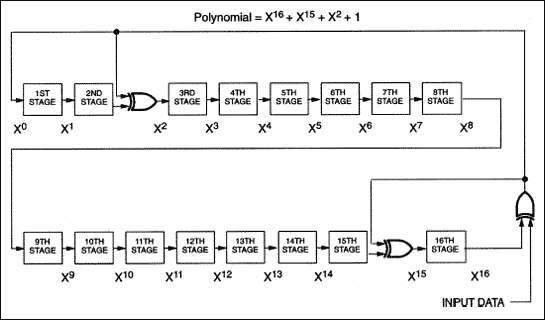
\includegraphics[scale=1]{CRC/explanation/CRC16.png}
\caption{}
\end{figure}

( The source of image: \url{https://olimex.wordpress.com/2014/01/10/weekend-programming-challenge-week-39-crc-16/} )

Only 3 XOR gates are present aside of shift register.

The following page has animation: \url{https://en.wikipedia.org/wiki/Computation_of_cyclic_redundancy_checks}.

It can be implemented maybe even using vacuum tubes.

And the task is not to compute remainder according to rules of arithmetics, but rather to detect errors.

Compare this to a division circuit with at least one binary adder/subtractor, which will have carry-ripple problem.
On the other hand, addition over GF(2) has no carries, hence, this problem absent.

\subsubsection{Further reading}

These documents I've found interesting/helpful:

\begin{itemize}

\item \url{http://www.ross.net/crc/download/crc_v3.txt}
\item \url{https://www.kernel.org/doc/Documentation/crc32.txt}
\item \url{http://web.archive.org/web/20161220015646/http://www.hackersdelight.org/crc.pdf}

\end{itemize}


\subsection{Factorize GF(2)/CRC polynomials}

GF(2)/CRC polynomials, like usual numbers, can also be factored, because a polynomial can be a product of two other polynomial (or not).

Some people say that good CRC polynomial should be irreducible (i.e., cannot be factored), some other say that this is not a requirement.
I've checked several CRC-16 and CRC-32 polynomials from \href{https://en.wikipedia.org/wiki/Cyclic_redundancy_check}{the Wikipedia article}.

% TODO \ref{}
The multiplier is constructed in the same manner, as I did it earlier for integer factorization using SAT.
Factors are not prime integers, but prime polynomials.

Another important thing to notice is that replacing XOR with addition will make this script factor integers, because addition in GF(2) is XOR.

Also, can be used for tests, online GF(2) polynomials factorization: \url{http://www.ee.unb.ca/cgi-bin/tervo/factor.pl?binary=101}.

\lstinputlisting[style=custompy]{CRC/factor/factor_GF2.py}


\subsection{Getting CRC polynomial and other CRC generator parameters}

Sometimes CRC implementations are incompatible with each other: polynomial and other parameters can be different.
Aside of polynomial, initial state can be either 0 or -1, final value can be inverted or not, endianness of the final value can be changed or not.
Trying all these parameters by hand to match with someone's else implementation can be a real pain.
Also, you can bruteforce 32-bit polynomial, but 64-bit polynomials is too much.

Deducing all these parameters is surprisingly simple using Z3, just get two values for 01 byte and 02, or any other bytes.

\lstinputlisting[style=custompy]{CRC/cracker/CRC_cracker.py}

This is for CRC-16:

\begin{lstlisting}
poly=0xa001, init=0x0, XORout=0
\end{lstlisting}

Sometimes, we have no enough information, but still can get something. This is for CRC-16-CCITT:

\begin{lstlisting}
poly=0xb30f, init=0x0, XORout=-1
poly=0x7c07, init=0x0, XORout==0, ReflectOut=true
poly=0x8408, init=0x0, XORout==0, ReflectOut=true
\end{lstlisting}

One of these results is correct.

We can get something even if we have only one result for one input byte:

\begin{lstlisting}[style=custompy]
# recipe-259177-1.py, CRC-64-ISO
width=64
samples=["\x01"]
must_be=[0x01B0000000000000]
sample_len=1
\end{lstlisting}

\begin{lstlisting}
poly=0x1fb12, init=0x0, XORout==0, ReflectOut=true
poly=0x1d24924924924924, init=0xffffffffffffffff, XORout=0
poly=0x86a9466cbb890d53, init=0x0, XORout=-1, ReflectOut=true
poly=0x580080, init=0x0, XORout==0, ReflectOut=true
poly=0xce9ce, init=0x0, XORout==0, ReflectOut=true
poly=0x53ffffffffffffff, init=0xffffffffffffffff, XORout=0
poly=0xd800000000000000, init=0x0, XORout=0
poly=0x38ad6, init=0x0, XORout==0, ReflectOut=true
poly=0x131e56e82623cae, init=0xffffffffffffffff, XORout==0, ReflectOut=true
poly=0x3fffffffffd3ffbf, init=0xffffffffffffffff, XORout==0, ReflectOut=true
poly=0x461861861861861, init=0xffffffffffffffff, XORout=0
total results 11
\end{lstlisting}

The files: \url{https://github.com/DennisYurichev/yurichev.com/...}.

The shortcoming: longer samples slows down everything significantly.
I had luck with samples up to 4 bytes, but no larger.

Further reading I've found interesting/helpful:

\begin{itemize}

\item \url{http://www.cosc.canterbury.ac.nz/greg.ewing/essays/CRC-Reverse-Engineering.html}
\item \url{http://reveng.sourceforge.net/crc-catalogue/1-15.htm}
\item \url{http://reveng.sourceforge.net/crc-catalogue/16.htm}
\item \url{http://reveng.sourceforge.net/crc-catalogue/17plus.htm}

\end{itemize}


\subsection{Finding (good) CRC polynomial}

Finding good CRC polynomial is tricky, and my results can't compete with other tested popular CRC polynomial.
Nevertheless, it was fun to use Z3 to find them.

I just generate 32 random samples, all has size between 1 and 32 bytes.
Then I flip 1..3 random bits and I add a constraint: CRC hash of the sample and hash of the modified sample (with 1..3 bits flipped) must differ.

\lstinputlisting{CRC/find_poly/CRC_find_poly.py}

Several polynomials for CRC8:

\begin{lstlisting}
poly=0xf9
poly=0x50
poly=0x90
...
\end{lstlisting}

... for CRC16:

\begin{lstlisting}
poly=0xf7af
poly=0x368
poly=0x268
poly=0x228
...
\end{lstlisting}

... for CRC32:

\begin{lstlisting}
poly=0x1683a5ab
poly=0x78553eda
poly=0x7a153eda
poly=0x7b353eda
...
\end{lstlisting}

... for CRC64:

\begin{lstlisting}
poly=0x8000000000000006
poly=0x926b19b536a62f10
poly=0x4a7bb0a7da78a370
poly=0xbbc781e7e83dabf0
...
\end{lstlisting}

Problem: at least this one. CRC must be able to detect errors in very long buffers, up to $2^{32}$ for CRC32. We can't feed that huge buffers to SMT solver.
I had success only with samples up to $\approx 32$ bytes.


\section{CRC (Cyclic redundancy check)}

\renewcommand{\CURPATH}{CRC/KLEE}

\subsection{Buffer alteration case \#1}

Sometimes, you need to alter a piece of data which is \emph{protected} by some kind of checksum or \ac{CRC}, and you can't change checksum or CRC value, but can alter piece of data so that checksum will remain the same.

Let's pretend, we've got a piece of data with ``Hello, world!'' string at the beginning and ``and goodbye'' string at the end.
We can alter 14 characters at the middle, but for some reason, they must be in \emph{a..z} limits, but we can put any characters there.
CRC64 of the whole block must be \TT{0x12345678abcdef12}.

Let's see\footnote{There are several slightly different CRC64 implementations, the one I use here can also be different from popular ones.}:

\lstinputlisting{\CURPATH/klee_CRC64.c}

Since our code uses memcmp() standard C/C++ function, we need to add \TT{--libc=uclibc} switch, so KLEE will use its own uClibc 
implementation. % \ref{} -> closed programs

\begin{lstlisting}
% clang -emit-llvm -c -g klee_CRC64.c

% time klee --libc=uclibc klee_CRC64.bc
\end{lstlisting}

It takes about 1 minute (on my Intel Core i3-3110M 2.4GHz notebook) and we getting this:

% FIXME:
\begin{lstlisting}
...
real    0m52.643s
user    0m51.232s
sys     0m0.239s
...
% ls klee-last | grep err
test000001.user.err
test000002.user.err
test000003.user.err
test000004.external.err

% ktest-tool --write-ints klee-last/test000004.ktest
ktest file : 'klee-last/test000004.ktest'
args       : ['klee_CRC64.bc']
num objects: 1
object    0: name: b'buf'
object    0: size: 46
object    0: data: b'Hello, world!.. qqlicayzceamyw ... and goodbye'
\end{lstlisting}

Maybe it's slow, but definitely faster than bruteforce.
Indeed, $log_2{26^{14}} \approx 65.8$
which is close to 64 bits.
In other words, one need $\approx 14$ latin characters to encode 64 bits.
And KLEE + \ac{SMT} solver needs 64 bits at some place it can alter to make final CRC64 value equal to what we defined.

I tried to reduce length of the \emph{middle block} to 13 characters: no luck for KLEE then, it has no space enough.

\subsection{Buffer alteration case \#2}

I went sadistic: what if the buffer must contain the CRC64 value which, after calculation of CRC64, will result in the same value?
Fascinatedly, KLEE can solve this.
The buffer will have the following format:

\begin{lstlisting}
Hello, world! <8 bytes (64-bit value)> and goodbye <6 more bytes>
\end{lstlisting}

\begin{lstlisting}
int main()
{
#define HEAD_STR "Hello, world!.. "
#define HEAD_SIZE strlen(HEAD_STR)
#define TAIL_STR " ... and goodbye"
#define TAIL_SIZE strlen(TAIL_STR)
// 8 bytes for 64-bit value:
#define MID_SIZE 8
#define BUF_SIZE HEAD_SIZE+TAIL_SIZE+MID_SIZE+6

	char buf[BUF_SIZE];
  
	klee_make_symbolic(buf, sizeof buf, "buf");

	klee_assume (memcmp (buf, HEAD_STR, HEAD_SIZE)==0);

	klee_assume (memcmp (buf+HEAD_SIZE+MID_SIZE, TAIL_STR, TAIL_SIZE)==0);
	
	uint64_t mid_value=*(uint64_t*)(buf+HEAD_SIZE);
	klee_assume (crc64 (0, buf, BUF_SIZE)==mid_value);

	klee_assert(0);

	return 0;
}
\end{lstlisting}

It works:

\begin{lstlisting}
% time klee --libc=uclibc klee_CRC64.bc
...
real    5m17.081s
user    5m17.014s
sys     0m0.319s

% ls klee-last | grep err
test000001.user.err
test000002.user.err
test000003.external.err

% ktest-tool --write-ints klee-last/test000003.ktest
ktest file : 'klee-last/test000003.ktest'
args       : ['klee_CRC64.bc']
num objects: 1
object    0: name: b'buf'
object    0: size: 46
object    0: data: b'Hello, world!.. T+]\xb9A\x08\x0fq ... and goodbye\xb6\x8f\x9c\xd8\xc5\x00'
\end{lstlisting}

8 bytes between two strings is 64-bit value which equals to CRC64 of this whole block.
Again, it's faster than brute-force way to find it.
If to decrease last spare 6-byte buffer to 4 bytes or less, KLEE works so long so I've stopped it.

\subsection{Recovering input data for given CRC32 value of it}

I've always wanted to do so, but everyone knows this is impossible for input buffers larger than 4 bytes.
As my experiments show, it's still possible for tiny input buffers of data, which is constrained in some way.

The CRC32 value of 6-byte ``SILVER'' string is known: \TT{0xDFA3DFDD}.
KLEE can find this 6-byte string, if it knows that each byte of input buffer is in \emph{A..Z} limits:

\lstinputlisting[numbers=left]{\CURPATH/klee_SILVER.c}

\begin{lstlisting}
% clang -emit-llvm -c -g klee_SILVER.c
...

% klee klee_SILVER.bc
...

% ls klee-last | grep err
test000013.external.err

% ktest-tool --write-ints klee-last/test000013.ktest
ktest file : 'klee-last/test000013.ktest'
args       : ['klee_SILVER.bc']
num objects: 1
object    0: name: b'str'
object    0: size: 6
object    0: data: b'SILVER'
\end{lstlisting}

Still, it's no magic: if to remove condition at lines 23..25 (i.e., if to relax constraints),
KLEE will produce some other string, which will be still correct for the CRC32 value given.

It works, because 6 Latin characters in \emph{A..Z} limits contain $\approx 28.2$ bits:
$log_2{26^6} \approx 28.2$, which is even smaller value than 32.
In other words, the final CRC32 value holds enough bits to recover $\approx 28.2$ bits of input.

The input buffer can be even bigger, if each byte of it will be in even tighter
constraints (decimal digits, binary digits, etc).

\subsection{In comparison with other hashing algorithms}

Things are that easy for some other hashing algorithms like \emph{Fletcher checksum},
but not for cryptographically secure ones (like MD5, SHA1, etc), they are protected from such simple cryptoanalysis.
See also: \ref{crypto}.




\chapter{MaxSMT}

%TODO write something

% subsections:
\section{Making smallest possible test suite using Z3}
\label{set_cover}

I once worked on rewriting large piece of code into pure C, and there were a tests, several thousands.
Testing process was painfully slow, so I thought if the test suite can be minimized somehow.

What we can do is to run each test and get code coverage
(information about which lines of code was executed and which are not).
Then the task is to make such test suite, where coverage is maximum, and number of tests is minimal.

In fact, this is \textit{set cover problem} (also known as \textit{hitting set problem}).
While simpler algorithms exist (see Wikipedia\footnote{\url{https://en.wikipedia.org/wiki/Set_cover_problem}}),
it is also possible to solve with SMT-solver.

First, I took \ac{LZSS} compression/decompression code
\footnote{\url{https://github.com/opensource-apple/kext_tools/blob/master/compression.c}} for the example,
from Apple sources.
Such routines are not easy to test.
Here is my version of it:
\url{https://github.com/DennisYurichev/SAT_SMT_by_example/blob/master/MaxSMT/set_cover/compression.c}.
I've added random generation of input data to be compressed.
Random generation is dependent of some kind of input seed.
Standard \TT{srand()}/\TT{rand()} are not recommended to be used, but for such simple task as ours, it's OK.
I'll generate\footnote{\url{https://github.com/DennisYurichev/yurichev.com/blob/master/blog/set_cover/gen_gcov_tests.sh}}
1000 tests with 0..999 seeds, that would produce random data to be compressed/decompressed/checked.

After the compression/decompression routine has finished its work,
GNU gcov utility is executed, which produces result like this:

\begin{lstlisting}
...
     3395:  189:        for (i = 1; i < F; i++) {
     3395:  190:            if ((cmp = key[i] - sp->text_buf[p + i]) != 0)
     2565:  191:                break;
        -:  192:        }
     2565:  193:        if (i > sp->match_length) {
     1291:  194:            sp->match_position = p;
     1291:  195:            if ((sp->match_length = i) >= F)
    #####:  196:                break;
        -:  197:        }
     2565:  198:    }
    #####:  199:    sp->parent[r] = sp->parent[p];
    #####:  200:    sp->lchild[r] = sp->lchild[p];
    #####:  201:    sp->rchild[r] = sp->rchild[p];
    #####:  202:    sp->parent[sp->lchild[p]] = r;
    #####:  203:    sp->parent[sp->rchild[p]] = r;
    #####:  204:    if (sp->rchild[sp->parent[p]] == p)
    #####:  205:        sp->rchild[sp->parent[p]] = r;
...
\end{lstlisting}

A leftmost number is an execution count for each line.
\TT{\#\#\#\#\#} means the line of code hasn't been executed at all.
The second column is a line number.

Now the Z3Py script, which will parse all these 1000 gcov results and produce minimal \textit{hitting set}:

\lstinputlisting[style=custompy]{MaxSMT/set_cover/set_cover.py}

And what it produces (\textasciitilde{}19s on my old Intel Quad-Core Xeon E3-1220 3.10GHz):

\begin{lstlisting}
% time python set_cover.py
sat
test_7
test_48
test_134
python set_cover.py  18.95s user 0.03s system 99% cpu 18.988 total
\end{lstlisting}

We need just these 3 tests to execute (almost) all lines in the code:
looks impressive, given the fact, that it would be notoriously hard to pick these tests by hand!
The result can be checked easily, again, using gcov utility.

This is sometimes also called MaxSAT/MaxSMT --- the problem is to find solution,
but the solution where some variable/expression is maximal as possible, or minimal as possible.

Also, the code gives incorrect results on Z3 4.4.1, but working correctly on Z3 4.5.0 (so please upgrade).
This is relatively fresh feature in Z3, so probably it was not stable in previous versions?

The files: \url{https://github.com/DennisYurichev/SAT_SMT_by_example/tree/master/MaxSMT/set_cover}.

Further reading:
\url{https://en.wikipedia.org/wiki/Set_cover_problem},
\url{https://en.wikipedia.org/wiki/Maximum_satisfiability_problem},
\url{https://en.wikipedia.org/wiki/Optimization_problem}.


\section{\ac{GCD} and \ac{LCM}}

\MathForProg has short explanation of GCD and LCM.

% subsubsections:
\subsection{\ac{GCD}}
\label{GCD}

To compute GCD, one of the oldest algorithms is used: \href{https://en.wikipedia.org/wiki/Euclidean_algorithm}{Euclidean algorithm}.
But, I can demonstrate how to make things much less efficient, but more spectacular.

To find GCD of 14 and 8, we are going to solve this system of equations:

% TODO texify
\begin{lstlisting}
x*GCD=14
y*GCD=8
\end{lstlisting}

Then we drop $x$ and $y$, we don't need them.
This system can be solved using paper and pencil, but GCD must be as big as possible.
Here we can use Z3 in MaxSMT mode:

\begin{lstlisting}
#!/usr/bin/env python

from z3 import *

opt = Optimize()

x,y,GCD=Ints('x y GCD')

opt.add(x*GCD==14)
opt.add(y*GCD==8)

h=opt.maximize(GCD)

print (opt.check())
print (opt.model())
\end{lstlisting}

That works:

\begin{lstlisting}
sat
[y = 4, x = 7, GCD = 2]
\end{lstlisting}

What if we need to find GCD for 3 numbers?
Maybe we are going to fill a space with biggest possible cubes?

\begin{lstlisting}
#!/usr/bin/env python

from z3 import *

opt = Optimize()

x,y,z,GCD=Ints('x y z GCD')

opt.add(x*GCD==300)
opt.add(y*GCD==333)
opt.add(z*GCD==900)

h=opt.maximize(GCD)

print (opt.check())
print (opt.model())
\end{lstlisting}

This is 3:

\begin{lstlisting}
sat
[z = 300, y = 111, x = 100, GCD = 3]
\end{lstlisting}

In SMT-LIB form:

\lstinputlisting[style=customsmt]{GCD_BV2.smt}


\subsection{Explanation of the Least Common Multiple}

Many people use \ac{LCM} in school. Sum up $\frac{1}{4}$ and $\frac{1}{6}$.
To find an answer mentally, you ought to find Lowest Common Denominator, which can be 4*6=24.
Now you can sum up $\frac{6}{24} + \frac{4}{24} = \frac{10}{24}$.

But the lowest denominator is also a LCM.
LCM of 4 and 6 is 12: $\frac{3}{12} + \frac{2}{12} = \frac{5}{12}$.

To find LCM of 4 and 6, we are going to solve the following diophantine (i.e., allowing only integer solutions) system of equations:

$4x = 6y = LCM$

... where LCM>0 and as small, as possible.

\begin{lstlisting}
#!/usr/bin/env python

from z3 import *

opt = Optimize()

x,y,LCM=Ints('x y LCM')

opt.add(x*4==LCM)
opt.add(y*6==LCM)
opt.add(LCM>0)

h=opt.minimize(LCM)

print (opt.check())
print (opt.model())
\end{lstlisting}

The (correct) answer:

\begin{lstlisting}
sat
[y = 2, x = 3, LCM = 12]
\end{lstlisting}




\subsection{Assignment problem}

I've found this at \url{http://www.math.harvard.edu/archive/20_spring_05/handouts/assignment_overheads.pdf} and took screenshot:

\begin{figure}[H]
\centering
\frame{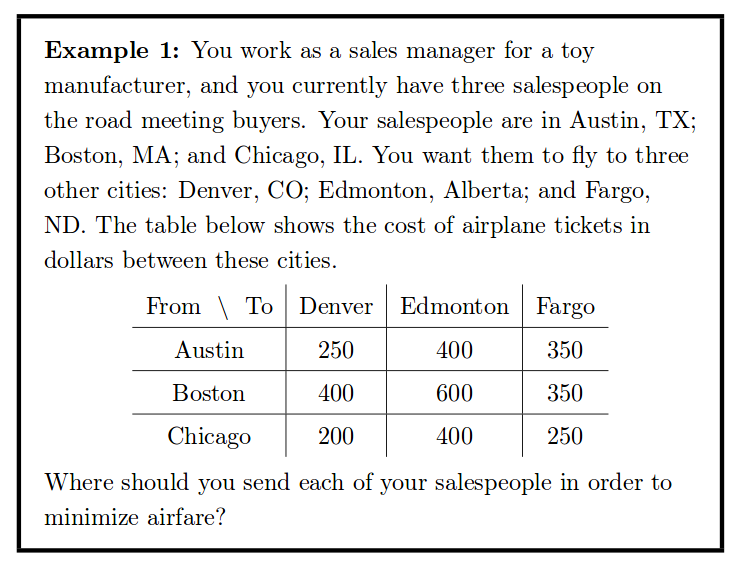
\includegraphics[scale=0.6]{MaxSMT/assign_problem/1.png}}
\end{figure}

As in my previous examples, Z3 and SMT-solver may be overkill for the task.
Simpler algorithm exists for this task (\textit{Hungarian algorithm/method})
\footnote{See also: \url{https://en.wikipedia.org/wiki/Hungarian_algorithm}.}.

But again, I use it to demonstrate the problem + as SMT-solvers demonstration.

Here is what I do:

\lstinputlisting[style=custompy]{MaxSMT/assign_problem/1.py}

In plain English this means \textit{choose such columns, so that their sum would be as small as possible}.

Result is seems to be correct:

\begin{lstlisting}
sat
[choice_0 = 1,
 choice_1 = 2,
 choice_2 = 0,
 z3name!12 = 0,
 z3name!7 = 1,
 z3name!10 = 2,
 z3name!8 = 0,
 z3name!11 = 0,
 z3name!9 = 0,
 final_sum = 950,
 row_value_2 = 200,
 row_value_1 = 350,
 row_value_0 = 400]
\end{lstlisting}

Again, as it is in the corresponding PDF presentation:

\begin{figure}[H]
\centering
\frame{\includegraphics[scale=0.6]{MaxSMT/assign_problem/2.png}}
\end{figure}

(However, I've no idea what ``z3name'' variables mean, perhaps, some internal variables?)


\section{Finding function minimum}
\label{func_minimum}

\lstinputlisting[style=customsmt]{MaxSMT/minimum/1959_AHSME_Problem_8.smt}


\subsection{Travelling salesman problem}

\renewcommand{\CURPATH}{MaxSMT/TSP}

This is it:

\lstinputlisting[style=custompy]{\CURPATH/TSP.py}

The result:

\begin{lstlisting}
sat
Dallas (1240 mi to the next city) ->
Los Angeles (831 mi to the next city) ->
Denver (700 mi to the next city) ->
Minneapolis (355 mi to the next city) ->
Chicago (713 mi to the next city) ->
New York (1374 mi to the next city) ->
distance_total= 5213 mi
\end{lstlisting}

Map I generated with Wolfram Mathematica:

\begin{figure}[H]
\centering
\includegraphics[scale=0.6]{\CURPATH/map1.png}
\caption{}
\end{figure}

Maximizing:

\begin{lstlisting}
sat
Dallas (862 mi to the next city) ->
Minneapolis (700 mi to the next city) ->
Denver (1631 mi to the next city) ->
New York (2451 mi to the next city) ->
Los Angeles (1745 mi to the next city) ->
Chicago (803 mi to the next city) ->
distance_total= 8192 mi
\end{lstlisting}

The map:

\begin{figure}[H]
\centering
\includegraphics[scale=0.6]{\CURPATH/map2.png}
\caption{}
\end{figure}

I could only process 6 cities, and it takes starting at several seconds up to 1 minute on my venerable Intel Quad-Core Xeon E3-1220 3.10GHz.
Perhaps, this is not a right tool for the job, well-known TSP algorithms way faster.

Even bruteforce enumeration is way faster ($6!=720$ paths).

However, it still can serve as demonstration.


\subsection{Clique in graph theory}

\renewcommand{\CURPATH}{MaxSMT/clique}

Graph is a group of nodes, some of them may be connected with each other, some are not.
One of the popular examples is the map of country: there are cities and roads.
"Cities" are called "nodes" or "vertices" in mathematics lingo, while "roads" are called "edges".
Another popular example of graph is computer network, including Internet.
Computer network is graph indeed, but it's closer to "sparse graph", because for the most part, computer networks are trees.

"Clique" in everyday speech (especially in political news) denotes a tight-knit group of people inside of some community.
In graph theory, "clique" is a subgraph (part of graph) each vertices ("nodes" or "members") of which are connected with each other.

\subsubsection{Social graph: simple example}

"Social graph" is a graph representing social links.
Here is example I made in Wolfram Mathematica:

\begin{lstlisting}
community = 
 Graph[{John <-> Mark, John <-> Alice, Mark <-> Alice, Tim <-> Alice, 
   Matthew <-> John, Matthew <-> Mark, Tim <-> John, Drake <-> Tim, 
   Bob <-> Drake, Bill <-> Mark, Bob <-> Alice, Tim <-> Mark}, 
  VertexLabels -> "Name"]
\end{lstlisting}

\begin{figure}[H]
\centering
\frame{\includegraphics[scale=0.7]{\CURPATH/graph1.png}}
\end{figure}

Let's try to find largest clique:

\begin{lstlisting}
In[]:= clique = FindClique[community]
Out[]= {{John, Mark, Alice, Tim}}
\end{lstlisting}

Indeed, each of these four persons is connected to each among other 3.
Wolfram Mathematica can highlight subgraph in graph:

\begin{lstlisting}
HighlightGraph[community, clique]
\end{lstlisting}

\begin{figure}[H]
\centering
\frame{\includegraphics[scale=0.7]{\CURPATH/graph2.png}}
\end{figure}

\subsubsection{Social graph: IRC network}

Internet Relay Chat (IRC) is popular among open-source developers.
One of the most popular IRC networks is Freenode.
And one of the most crowded IRC channel there is \#ubuntu, devoted to Ubuntu Linux.
I used data from it, because all logs are available (starting at 2004), for example:
\url{http://irclogs.ubuntu.com/2015/01/01/%23ubuntu.txt}.

When someone asks, and someone another going to answer the question, IRC users are address each other in this way:

\begin{lstlisting}
[00:11] <synire> How would one find the path of an application installed using terminal?
[00:11] <zykotick9> synire: "whereis foo"
[00:11] <synire> zykotick9: thanks!
\end{lstlisting}

It's not a rule, but well-established practice, so we can recover the information, which users talks to which users most often.
Let's say, we would build a link between two IRC users if 
1) they talk to each other at least 10-11 days (not necessary consequent);
2) do this at least 6 months (not necessary consequent).

The largest cliques of \#ubuntu IRC channel in 10-11 years period are these:

\begin{lstlisting}
* clique size 11
['ubottu', 'ActionParsnip', 'ikonia', 'Ben64', 'zykotick9', 'theadmin', 'dr_willis', 'MonkeyDust', 'usr13', 'bekks', 'iceroot']
* clique size 10
['ubottu', 'ActionParsnip', 'ikonia', 'jrib', 'bazhang', 'Pici', 'iceroot', 'theadmin', 'IdleOne', 'erUSUL']
* clique size 10
['ubottu', 'ActionParsnip', 'ikonia', 'jrib', 'bazhang', 'Pici', 'iceroot', 'theadmin', 'zykotick9', 'usr13']
* clique size 10
['ubottu', 'ActionParsnip', 'ikonia', 'jrib', 'bazhang', 'Pici', 'iceroot', 'sebsebseb', 'IdleOne', 'erUSUL']
* clique size 10
['ubottu', 'ActionParsnip', 'ikonia', 'jrib', 'Dr_Willis', 'Pici', 'edbian', 'IdleOne', 'Jordan_U', 'theadmin']
* clique size 10
['ubottu', 'ActionParsnip', 'ikonia', 'jrib', 'Dr_Willis', 'Pici', 'edbian', 'IdleOne', 'Jordan_U', 'sebsebseb']
* clique size 10
['ubottu', 'ActionParsnip', 'ikonia', 'jrib', 'Dr_Willis', 'Pici', 'erUSUL', 'iceroot', 'IdleOne', 'theadmin']
* clique size 10
['ubottu', 'ActionParsnip', 'ikonia', 'jrib', 'Dr_Willis', 'Pici', 'erUSUL', 'iceroot', 'IdleOne', 'sebsebseb']
* clique size 10
['ubottu', 'ActionParsnip', 'ikonia', 'jrib', 'Dr_Willis', 'Pici', 'erUSUL', 'iceroot', 'ubuntu', 'sebsebseb']
* clique size 10
['ubottu', 'ActionParsnip', 'ikonia', 'Ben64', 'histo', 'bekks', 'MonkeyDust', 'dr_willis', 'iceroot', 'usr13']
...
\end{lstlisting}

% FIXME
Perhaps, these users are frequenters of the channel. List of all cliques are here:
\url{\GitHubBlobMasterURL/\CURPATH/files/IRC/results.txt}.
The output is not terse, because all listed cliques are cliques indeed, and single user or users group can be member of several cliques, that's correct.
Cliques can be overlapped and be members of bigger cliques.
It's possible to produce more human-like results using 
\href{https://en.wikipedia.org/wiki/Community_structure#Algorithms_for_finding_communities}{more complex algorithms for finding communities}.

The source code of my scripts here: \url{\GitHubTreeMasterURL/\CURPATH/files/IRC}.
I used the excellent \href{https://networkx.github.io/}{networkx graph library}.

\subsubsection{Attempt to find communities in IRC social graph}

Wolfram Mathematica can try to find communities within social graph.
Here I will import information about all IRC interactions from the start of 2013 till the summer of 2015.
User nicknames are coded by numbers for simplicity.

\begin{lstlisting}
In[]:= g2 = 
 Graph[{91708 -> 93574, 93414 -> 91525, 93414 -> 89579, 
   90407 -> 93896, 93414 -> 93598, 93809 -> 5909, 93698 -> 93801, 
   93163 -> 83317, 84930 -> 93896, 93414 -> 92947, 93414 -> 91708, 
   93792 -> 92887, 84930 -> 91708, 91708 -> 84930, 88400 -> 93698, 
   ...
   93809 -> 93475, 93698 -> 92887, 93801 -> 93670, 92887 -> 93598}]
\end{lstlisting}

The resulting graph is:

\begin{figure}[H]
\centering
\frame{\includegraphics[scale=0.5]{\CURPATH/IRC_g2.png}}
\end{figure}

There some artifacts (at the bottom) which can be ignored so far, I think.
There is prominent centers: one huge and two others are smaller.
I'm not sure, but I can suggest these parts of graph are just users who has different sleep paterns, or, more likely, from different time zones,
so each important time zone (like Americas, Europe, Asia/Oceania) may have their own social communities.
But again, I'm not sure, this should be investigated first.

Let's try to find communities and hightlight them within the graph:

\begin{lstlisting}
c2 = FindGraphCommunities[g2];
HighlightGraph[g2, Map[Subgraph[g2, #] &, c2]]
\end{lstlisting}

\begin{figure}[H]
\centering
\frame{\includegraphics[scale=0.5]{\CURPATH/IRC_c2.png}}
\end{figure}

Hard to say if Mathematica right, but this is what it did.

Now let's take the whole graph of all IRC interactions starting at year 2004 till the summer of 2015.
The graph is much bigger:

\begin{figure}[H]
\centering
\frame{\includegraphics[scale=0.5]{\CURPATH/IRC_g1.png}}
\end{figure}

There are more artifacts.

Let's apply Mathematica's method to find communities:

\begin{figure}[H]
\centering
\frame{\includegraphics[scale=0.5]{\CURPATH/IRC_c1.png}}
\end{figure}

Is it right? Maybe. Needless to say, since timespan is so long (at least 10 years), we can belive that some communities which may exists in 2004-2006 may be
extinct in 2014-2015 (people got older, lost their interest in Ubuntu Linux, etc), but they all are visible on this graph.

Summary: perhaps, on our next experiment we should filter out IRC data by years and time zones.

\subsubsection{Social graph: social networks}

Perhaps, social networking websites like Facebook and Twitter in the "people you may know" tab shows you users of most populous (by your current friends) cliques.
It may be much more complex in reality, but nevertheless, this is simplest possible way to offer you new social contacts.

\subsubsection{Links graph: Wikipedia}

Wikipedia has a lot of internal links, ~463,000,000 in English Wikipedia as of summer 2015, if not to count user/talk/media pages, etc.
It's possible to build a graph where Wikipedia article is a vertice (or node) and a link from one article to another is edge.
By link between articles we would call the case when the first article has the link to the second article, but also the second has the link to the first one.

Here are some examples of cliques I found this way. Number in parenthesis is clique size.

\begin{itemize}

\item
Chess-related articles (9): Reuben Fine, Mikhail Botvinnik, Samuel Reshevsky, Max Euwe, FIDE, Alexander Alekhine, World Chess Championship, José Raúl Capablanca, AVRO 1938 chess tournament.

\item
Utah-related articles (9): Red Line (TRAX), Utah Transit Authority, Blue Line (TRAX), TRAX (light rail), Salt Lake City, Green Line (TRAX), FrontRunner, University of Utah, Utah.

\item
Articles related to Doctor Who (9): Doctor Who (film), Doctor Who, The Doctor (Doctor Who), Eighth Doctor, The Master (Doctor Who), Gallifrey, TARDIS, Doctor Who Magazine, Seventh Doctor.

\item
Space (9): New Horizons, Pioneer 11, Voyager 1, Europa (moon), Callisto (moon), Ganymede (moon), Jupiter, Io (moon), Pioneer 10.

\item
Hip hop music (9): G-funk, Dr. Dre, Death Row Records, Snoop Dogg, The Chronic, Gangsta rap, West Coast hip hop, N.W.A, Hip hop music.

\item
Metal music (9): Master of Puppets, Thrash metal, Cliff Burton, James Hetfield, Kirk Hammett, Metallica, Kill 'Em All, Ride the Lightning, Dave Mustaine.

\item
The Beatles (8): Break-up of the Beatles, The Beatles, George Harrison, Let It Be, John Lennon, Paul McCartney, Ringo Starr, Abbey Road.

\end{itemize}

Each Wikipedia article within any of these cliques has links to each article in clique.

Full lists of first 1000 largest cliques in English, Russian and Ukrainian Wikipedias plus source code of my scripts is here:
\url{\GitHubTreeMasterURL/\CURPATH/files/wikipedia}.

\subsubsection{Social graph: LiveJournal spammers}

LiveJournal is popular blogging platform in Russian-speaking Internet, which, as any other platform, flooded by spammers.
I once tried, for experiment, to find a way to make distinction between them and human users.
(I did this in 2010-2011, so this information may be not relevant these days).

Aside of false texts spammers posted to their blogs, spammers also mutually friended may spam accounts, so it was not unusual to register, let's say, 1000 fake
accounts and friend each other.

If to build a graph of all links between LiveJournal users, and find largest cliques, there will be prominent unusually large cliques of LiveJournal users, 
up to ~1000.
In real world, you would not easliy find a social group of ~1000 persons who keeps mutual links with each other 
(there is interesting reading about it: \href{https://en.wikipedia.org/w/index.php?title=Dunbar%27s_number}{Dunbar's number}).

Well, spammers could lower this number, so each fake user would have 100-200 mutual friends instead of ~1000 (which is less suspicious), but still, 
cliques were too perfect: each node connected to each other with very low
amount of "external" links, leading to other spammer's cliques and human users.

\subsubsection{Links graph: link farms}

Talking about spammers, there was (or maybe still used today?) also a Black Hat SEO method to build 
"link farms":
this is a collection of many websites which has links to each other.
Interestingly, if you analyze link graph and find cliques, such farms are clearly visible.


\subsection{Find maximal clique using Open-WBO}

\renewcommand{\CURPATH}{MaxSMT/clique_openwbo}

Though not efficient method, but very spectacular.

Given the 50-vertices graph: \url{\GitHubBlobMasterURL/\CURPATH/edges.txt}.

\lstinputlisting[style=custompy]{\CURPATH/1.py}

Resulting WCNF file:

\lstinputlisting{\CURPATH/1.wcnf}

And the (correct) result, however, not the single one:

\lstinputlisting{\CURPATH/r.txt}




\chapter{Program synthesis}

Program synthesis is a process of automatic program generation, in accordance with some specific goals.

% subsections:
\subsection{Synthesis of simple program using Z3 SMT-solver}
\label{synth_mult}

Sometimes, multiplication operation can be replaced with a several operations of shifting/addition/subtraction.
Compilers do so, because pack of instructions can be executed faster.

For example, multiplication by 19 is replaced by GCC 5.4 with pair of instructions: \TT{lea edx, [eax+eax*8]} and\\
\TT{lea eax, [eax+edx*2]}.
This is sometimes also called ``superoptimization''.

Let's see if we can find a shortest possible instructions pack for some specified multiplier.

As I've already wrote once, SMT-solver can be seen as a solver of huge systems of equations.
The task is to construct such system of equations, which, when solved, could produce a short program.
I will use electronics analogy here, it can make things a little simpler.

First of all, what our program will be consting of? There will be 3 operations allowed: ADD/SUB/SHL.
Only registers allowed as operands, except for the second operand of SHL (which could be in 1..31 range).
Each register will be assigned only once (as in \ac{SSA}).

And there will be some ``magic block'', which takes all previous register states, it also takes operation type,
operands and produces a value of next register's state.

\begin{lstlisting}
	        op ------------+
	        op1_reg -----+ |
	        op2_reg ---+ | |
	                   | | |
	                   v v v
	             +---------------+
	             |               |
	registers -> |               | -> new register's state
	             |               |
	             +---------------+
\end{lstlisting}

Now let's take a look on our schematics on top level:

\begin{lstlisting}
	0 -> blk -> blk -> blk .. -> blk -> 0

	1 -> blk -> blk -> blk .. -> blk -> multiplier
\end{lstlisting}

Each block takes previous state of registers and produces new states.
There are two chains.
First chain takes 0 as state of R0 at the very beginning, and the chain is supposed to produce 0 at the end
(since zero multiplied by any value is still zero).
The second chain takes 1 and must produce multiplier as the state of very last register
(since 1 multiplied by multiplier must equal to multiplier).

Each block is ``controlled'' by operation type, operands, etc.
For each column, there is each own set.

Now you can view these two chains as two equations.
The ultimate goal is to find such state of all operation types and operands, so the first chain will equal to 0,
and the second to multiplier.

Let's also take a look into ``magic block'' inside:

\begin{lstlisting}
	                op1_reg         op
	                   |            v
	                   v         +-----+
	registers ---> selector1 --> | ADD |
	           +                 | SUB | ---> result
	           |                 | SHL |
	           +-> selector2 --> +-----+
	                  ^             ^
	                  |             |
	               op2_reg       op2_imm
\end{lstlisting}

Each selector can be viewed as a simple multipositional switch.
If operation is SHL, a value in range of 1..31 is used as second operand.

So you can imagine this electric circuit and your goal is to turn all switches in such a state, so two chains
will have 0 and multiplier on output.
This sounds like logic puzzle in some way.
Now we will try to use Z3 to solve this puzzle.

First, we define all varibles:

\begin{lstlisting}
R=[[BitVec('S_s%d_c%d' % (s, c), 32) for s in range(MAX_STEPS)] for c in range (CHAINS)]
op=[Int('op_s%d' % s) for s in range(MAX_STEPS)]
op1_reg=[Int('op1_reg_s%d' % s) for s in range(MAX_STEPS)]
op2_reg=[Int('op2_reg_s%d' % s) for s in range(MAX_STEPS)]
op2_imm=[BitVec('op2_imm_s%d' % s, 32) for s in range(MAX_STEPS)]
\end{lstlisting}

R[][] is registers state for each chain and each step.\\
On contrary, \TT{op}/\TT{op1\_reg}/\TT{op2\_reg}/\TT{op2\_imm} variables are defined for each step, but for both chains,
since both chains at each column has the same operation/operands.

Now we must limit count of operations, and also, register's number for each step must not be bigger than step number,
in other words, instruction at each step is allowed to access only registers which were already set before:

\begin{lstlisting}
for s in range(1, STEPS):
    # for each step
    sl.add(And(op[s]>=0, op[s]<=2))
    sl.add(And(op1_reg[s]>=0, op1_reg[s]<s))
    sl.add(And(op2_reg[s]>=0, op2_reg[s]<s))
    sl.add(And(op2_imm[s]>=1, op2_imm[s]<=31))
\end{lstlisting}

Fix register of first step for both chains:

\begin{lstlisting}
for c in range(CHAINS):
    # for each chain:
    sl.add(R[c][0]==chain_inputs[c])
    sl.add(R[c][STEPS-1]==chain_inputs[c]*multiplier)
\end{lstlisting}

Now let's add ``magic blocks'':

\begin{lstlisting}
for s in range(1, STEPS):
    sl.add(R[c][s]==simulate_op(R,c, op[s], op1_reg[s], op2_reg[s], op2_imm[s]))
\end{lstlisting}

Now how ``magic block'' is defined?

\begin{lstlisting}
def selector(R, c, s):
    # for all MAX_STEPS:
    return If(s==0, R[c][0],
	    If(s==1, R[c][1],
            If(s==2, R[c][2],
	    If(s==3, R[c][3],
            If(s==4, R[c][4],
            If(s==5, R[c][5],
	    If(s==6, R[c][6],
            If(s==7, R[c][7],
	    If(s==8, R[c][8],
            If(s==9, R[c][9],
	        0)))))))))) # default

def simulate_op(R, c, op, op1_reg, op2_reg, op2_imm):
    op1_val=selector(R,c,op1_reg)
    return If(op==0, op1_val + selector(R, c, op2_reg),
	   If(op==1, op1_val - selector(R, c, op2_reg),
           If(op==2, op1_val << op2_imm,
	       0))) # default
\end{lstlisting}

This is very important to understand: if the operation is ADD/SUB, \TT{op2\_imm}'s value is just ignored.
Otherwise, if operation is SHL, value of \TT{op2\_reg} is ignored.
Just like in case of digital circuit.

The code: \url{https://github.com/DennisYurichev/SAT_SMT_by_example/blob/master/pgm_synth/mult/mult.py}.

Now let's see how it works:

\begin{lstlisting}
% ./mult.py 12
multiplier= 12
attempt, STEPS= 2
unsat
attempt, STEPS= 3
unsat
attempt, STEPS= 4
sat!
r1=SHL r0, 2
r2=SHL r1, 1
r3=ADD r1, r2
tests are OK
\end{lstlisting}

The first step is always a step containing 0/1, or, r0.
So when our solver reporting about 4 steps, this means 3 instructions.

Something harder:

\begin{lstlisting}
% ./mult.py 123
multiplier= 123
attempt, STEPS= 2
unsat
attempt, STEPS= 3
unsat
attempt, STEPS= 4
unsat
attempt, STEPS= 5
sat!
r1=SHL r0, 2
r2=SHL r1, 5
r3=SUB r2, r1
r4=SUB r3, r0
tests are OK
\end{lstlisting}

Now the code multiplying by 1234:

\begin{lstlisting}
r1=SHL r0, 6
r2=ADD r0, r1
r3=ADD r2, r1
r4=SHL r2, 4
r5=ADD r2, r3
r6=ADD r5, r4
\end{lstlisting}

Looks great, but it took $\approx 23$ seconds to find it on my Intel Xeon CPU E31220 @ 3.10GHz.
I agree, this is far from practical usage.
Also, I'm not quite sure that this piece of code will work faster than a single multiplication instruction.
But anyway, it's a good demonstration of SMT solvers capabilities.

The code multiplying by 12345 ($\approx 150$ seconds):

\begin{lstlisting}
r1=SHL r0, 5
r2=SHL r0, 3
r3=SUB r2, r1
r4=SUB r1, r3
r5=SHL r3, 9
r6=SUB r4, r5
r7=ADD r0, r6
\end{lstlisting}

Multiplication by 123456 ($\approx 8$ minutes!):

\begin{lstlisting}
r1=SHL r0, 9
r2=SHL r0, 13
r3=SHL r0, 2
r4=SUB r1, r2
r5=SUB r3, r4
r6=SHL r5, 4
r7=ADD r1, r6
\end{lstlisting}

\subsubsection{Few notes}

I've removed SHR instruction support, simply because the code multiplying by a constant makes no use of it.
Even more: it's not a problem to add support of constants as second operand for all instructions,
but again, you wouldn't find a piece of code which does this job and uses some additional constants.
Or maybe I wrong?

Of course, for another job you'll need to add support of constants and other operations.
But at the same time, it will work slower and slower.
So I had to keep \ac{ISA} of this toy \ac{CPU} as compact as possible.

\subsubsection{The code}

\url{https://github.com/DennisYurichev/SAT_SMT_by_example/blob/master/pgm_synth/mult}.


\section{Rockey dongle: finding unknown algorithm using only input/output pairs}

(This text was first published in August 2012 in my blog: \url{http://blog.yurichev.com/node/71}.)

Some smartcards can execute Java or .NET code - that's the way to hide your sensitive algorithm
into chip that is very hard to break (decapsulate).
For example, one may encrypt/decrypt data files by hidden crypto algorithm rendering software
piracy of such software close to impossible --- an encrypted date file created on software with connected smartcard
would be impossible to decrypt on cracked version of the same software.
(This leads to many nuisances, though.)

That's what is called \emph{black box}.

Some software protection dongles offers this functionality too.
One example is Rockey 4\footnote{\url{http://www.rockey.nl/en/rockey.html}}.

\begin{figure}[H]
\centering
\includegraphics[scale=2]{pgm_synth/rockey/rockey_4.jpg}
\caption{Rockey 4 dongle}
\end{figure}

This is a small dongle connected via USB. Is contain some user-defined memory but also memory for user algorithms.

The virtual (toy) CPU for these algorithms is very simple: it offer only 8 16-bit registers
(however, only 4 can be set and read) and 8 operations
(addition, subtractation, cyclic left shifting, multiplication, OR, XOR, AND, negation).

Second instruction argument can be a constant (from 0 to 63) instead of register.

Each algorithm is described by string like \\
\TT{A=A+B, B=C*13, D=D\^{}A, C=B*55, C=C\&A, D=D|A, A=A*9, A=A\&B}.

There are no memory, stack, conditional/unconditional jumps, etc.

Each algorithm, obviously, can't have side effects, so they are actually \emph{pure functions}
and their results can be \emph{memoized}.

By the way, as it has been mentioned in Rockey 4 manual, first and last instruction cannot have constants.
Maybe that's because these fields used for some internal data:
each algorithm start and end should be marked somehow internally anyway.

Would it be possible to reveal hidden impossible-to-read algorithm only by recording input/output dongle traffic?
Common sense tell us ``no''. But we can try anyway.

Since, my goal wasn't to break into some Rockey-protected software,
I was interesting only in limits (which algorithms could we find),
so I make some things simpler: we will work with only 4 16-bit registers,
and there will be only 6 operations (add, subtract, multiply, OR, XOR, AND).

Let's first calculate, how much information will be used in brute-force case.

There are 384 of all possible instructions in \TT{reg=reg,op,reg} format for 4 registers and 6 operations,
and also 6144 instructions in \TT{reg=reg,op,constant} format.
Remember that constant limited to 63 as maximal value? That help us for a little.

So, there are 6528 of all possible instructions.
This mean, there are $\approx 1.1 \cdot 10^{19}$ 5-instruction algorithms.
That's too much.

How can we express each instruction as system of equations?
While remembering some school mathematics, I wrote this:

\begin{lstlisting}
Function one\_step()=

# Each Bx is integer, but may be only 0 or 1.

# only one of B1..B4 and B5..B9 can be set
reg1=B1*A + B2*B + B3*C + B4*D
reg_or_constant2=B5*A + B6*B + B7*C + B8*D + B9*constant
reg1 should not be equal to reg_or_constant2

# Only one of B10..B15 can be set
result=result+B10*(reg1*reg2)
result=result+B11*(reg1^reg2)
result=result+B12*(reg1+reg2)
result=result+B13*(reg1-reg2)
result=result+B14*(reg1|reg2)
result=result+B15*(reg1&reg2)

B16 - true if register isn't updated in this part
B17 - true if register is updated in this part
(B16 cannot be equal to B17)
A=B16*A + B17*result
B=B18*A + B19*result
C=B20*A + B21*result
D=B22*A + B23*result
\end{lstlisting}

That's how we can express each instruction in algorithm.

5-instructions algorithm can be expressed like this:\\
\TT{one\_step (one\_step (one\_step (one\_step (one\_step (input\_registers)))))}.

Let's also add five known input/output pairs and we'll get system of equations like this:

\begin{lstlisting}
one_step (one_step (one_step (one_step (one_step (input_1)))))==output_1
one_step (one_step (one_step (one_step (one_step (input_2)))))==output_2
one_step (one_step (one_step (one_step (one_step (input_3)))))==output_3
one_step (one_step (one_step (one_step (one_step (input_4)))))==output_4
.. etc
\end{lstlisting}

So the question now is to find $5 \cdot 23$ boolean values satisfying known input/output pairs.

I wrote small utility to probe Rockey 4 algorithm with random numbers, it produce results in form:

\begin{lstlisting}
RY_CALCULATE1: (input) p1=30760 p2=18484 p3=41200 p4=61741 (output) p1=49244 p2=11312 p3=27587 p4=12657
RY_CALCULATE1: (input) p1=51139 p2=7852 p3=53038 p4=49378 (output) p1=58991 p2=34134 p3=40662 p4=9869
RY_CALCULATE1: (input) p1=60086 p2=52001 p3=13352 p4=45313 (output) p1=46551 p2=42504 p3=61472 p4=1238
RY_CALCULATE1: (input) p1=48318 p2=6531 p3=51997 p4=30907 (output) p1=54849 p2=20601 p3=31271 p4=44794
\end{lstlisting}

p1/p2/p3/p4 are just another names for A/B/C/D registers.

Now let's start with Z3. We will need to express Rockey 4 toy CPU in Z3Py (Z3 Python \ac{API}) terms.

It can be said, my Python script is divided into two parts: 

\begin{itemize}
\item constraint definitions (like, \emph{output\_1 should be $n$ for input\_1=m},
\emph{constant cannot be greater than 63}, etc); 

\item functions constructing system of equations.
\end{itemize}

This piece of code define some kind of \emph{structure} consisting of 4 named 16-bit variables,
each represent register in our toy CPU.

\begin{lstlisting}
Registers_State=Datatype ('Registers_State')
Registers_State.declare('cons', ('A', BitVecSort(16)), ('B', BitVecSort(16)), ('C', BitVecSort(16)), ('D', BitVecSort(16)))
Registers_State=Registers_State.create()
\end{lstlisting}

These enumerations define two new types (or \emph{sorts} in Z3's terminology):

\begin{lstlisting}
Operation, (OP_MULT, OP_MINUS, OP_PLUS, OP_XOR, OP_OR, OP_AND) = EnumSort('Operation', ('OP_MULT', 'OP_MINUS', 'OP_PLUS', 'OP_XOR', 'OP_OR', 'OP_AND'))

Register, (A, B, C, D) = EnumSort('Register', ('A', 'B', 'C', 'D'))
\end{lstlisting}

This part is very important, it defines all variables in our system of equations. 
\TT{op\_step} is type of operation in instruction.
\TT{reg\_or\_constant} is selector between register and constant in second argument ---
\emph{False} if it's a register and \emph{True} if it's a constant. 
\TT{reg\_step} is a destination register of this instruction. 
\TT{reg1\_step} and \TT{reg2\_step} are just registers at arg1 and arg2. 
\TT{constant\_step} is constant (in case it's used in instruction instead of arg2).

\begin{lstlisting}
op_step=[Const('op_step%s' % i, Operation) for i in range(STEPS)]
reg_or_constant_step=[Bool('reg_or_constant_step%s' % i) for i in range(STEPS)]
reg_step=[Const('reg_step%s' % i, Register) for i in range(STEPS)]
reg1_step=[Const('reg1_step%s' % i, Register) for i in range(STEPS)]
reg2_step=[Const('reg2_step%s' % i, Register) for i in range(STEPS)]
constant_step = [BitVec('constant_step%s' % i, 16) for i in range(STEPS)]
\end{lstlisting}

Adding constraints is very simple. Remember, I wrote that each constant cannot be larger than 63?

\begin{lstlisting}
# according to Rockey 4 dongle manual, arg2 in first and last instructions cannot be a constant
s.add (reg_or_constant_step[0]==False)
s.add (reg_or_constant_step[STEPS-1]==False)

...

for x in range(STEPS):
   s.add (constant_step[x]>=0, constant_step[x]<=63)
\end{lstlisting}

Known input/output values are added as constraints too.

Now let's see how to construct our system of equations:

\begin{lstlisting}
# Register, Registers_State -> int
def register_selector (register, input_registers):
    return If(register==A, Registers_State.A(input_registers),
           If(register==B, Registers_State.B(input_registers), 
           If(register==C, Registers_State.C(input_registers), 
           If(register==D, Registers_State.D(input_registers), 
                           0)))) # default
\end{lstlisting}

This function returning corresponding register value from \emph{structure}.
Needless to say, the code above is not executed. 
\TT{If()} is Z3Py function. 
The code only declares the function, which will be used in another. 
Expression declaration resembling LISP \ac{PL} in some way.

Here is another function where \TT{register\_selector()} is used:

\begin{lstlisting}
# Bool, Register, Registers_State, int -> int
def register_or_constant_selector (register_or_constant, register, input_registers, constant): 
    return If(register_or_constant==False, register_selector(register, input_registers), constant)
\end{lstlisting}

The code here is never executed too. 
It only constructs one small piece of very big expression. 
But for the sake of simplicity, one can think all these functions will be called during bruteforce search, many times,
at fastest possible speed.

\begin{lstlisting}
# Operation, Bool, Register, Register, Int, Registers_State -> int
def one_op (op, register_or_constant, reg1, reg2, constant, input_registers):
    arg1=register_selector(reg1, input_registers)
    arg2=register_or_constant_selector (register_or_constant, reg2, input_registers, constant)
    return If(op==OP_MULT,   arg1*arg2,
           If(op==OP_MINUS,  arg1-arg2,
           If(op==OP_PLUS,   arg1+arg2, 
           If(op==OP_XOR,    arg1^arg2, 
           If(op==OP_OR,     arg1|arg2, 
           If(op==OP_AND,    arg1&arg2, 
                          0)))))) # default
\end{lstlisting}

Here is the expression describing each instruction. 
\TT{new\_val} will be assigned to destination register,
while all other registers' values are copied from input registers' state:

\begin{lstlisting}
# Bool, Register, Operation, Register, Register, Int, Registers_State -> Registers_State
def one_step (register_or_constant, register_assigned_in_this_step, op, reg1, reg2, constant, input_registers):
    new_val=one_op(op, register_or_constant, reg1, reg2, constant, input_registers)
    return If (register_assigned_in_this_step==A, Registers_State.cons (new_val,
                                                                        Registers_State.B(input_registers), 
                                                                        Registers_State.C(input_registers), 
                                                                        Registers_State.D(input_registers)),
           If (register_assigned_in_this_step==B, Registers_State.cons (Registers_State.A(input_registers), 
                                                                        new_val,
                                                                        Registers_State.C(input_registers),
                                                                        Registers_State.D(input_registers)), 
           If (register_assigned_in_this_step==C, Registers_State.cons (Registers_State.A(input_registers), 
                                                                        Registers_State.B(input_registers), 
                                                                        new_val,
                                                                        Registers_State.D(input_registers)), 
           If (register_assigned_in_this_step==D, Registers_State.cons (Registers_State.A(input_registers), 
                                                                        Registers_State.B(input_registers), 
                                                                        Registers_State.C(input_registers), 
                                                                        new_val),
                                                  Registers_State.cons(0,0,0,0))))) # default
\end{lstlisting}

This is the last function describing a whole $n$-step program:

\begin{lstlisting}
def program(input_registers, STEPS):
    cur_input=input_registers
    for x in range(STEPS):
        cur_input=one_step (reg_or_constant_step[x], reg_step[x], op_step[x], reg1_step[x], reg2_step[x], constant_step[x], cur_input)
    return cur_input
\end{lstlisting}

Again, for the sake of simplicity, it can be said, now Z3 will try each possible
registers/operations/constants against this expression to find such combination which satisfy all input/output pairs. 
Sounds absurdic, but this is close to reality.
SAT/SMT-solvers indeed tries them all.
But the trick is to prune search tree as early as possible, so it will work for some reasonable time.
And this is hardest problem for solvers.

Now let's start with very simple 3-step algorithm: \TT{B=A\^{}D, C=D*D, D=A*C}.
Please note: register \TT{A} left unchanged.
I programmed Rockey 4 dongle with the algorithm, and recorded algorithm outputs are:

\begin{lstlisting}
RY_CALCULATE1: (input) p1=8803 p2=59946 p3=36002 p4=44743 (output) p1=8803 p2=36004 p3=7857 p4=24691
RY_CALCULATE1: (input) p1=5814 p2=55512 p3=52155 p4=55813 (output) p1=5814 p2=52403 p3=33817 p4=4038
RY_CALCULATE1: (input) p1=25206 p2=2097 p3=55906 p4=22705 (output) p1=25206 p2=15047 p3=10849 p4=43702
RY_CALCULATE1: (input) p1=10044 p2=14647 p3=27923 p4=7325 (output) p1=10044 p2=15265 p3=47177 p4=20508
RY_CALCULATE1: (input) p1=15267 p2=2690 p3=47355 p4=56073 (output) p1=15267 p2=57514 p3=26193 p4=53395
\end{lstlisting}

It took about one second and only 5 pairs above to find algorithm
(on my quad-core Xeon E3-1220 3.1GHz, however, Z3 solver working in single-thread mode):

\begin{lstlisting}
B = A ^ D
C = D * D
D = C * A
\end{lstlisting}

Note the last instruction: \TT{C} and \TT{A} registers are swapped comparing to version I wrote by hand. 
But of course, this instruction is working in the same way, because multiplication is commutative operation.

Now if I try to find 4-step program satisfying to these values, my script will offer this:

\begin{lstlisting}
B = A ^ D
C = D * D
D = A * C
A = A | A
\end{lstlisting}

\dots and that's really fun, because the last instruction do nothing with value in register \TT{A},
it's like \ac{NOP}---but still, algorithm is correct for all values given.

Here is another 5-step algorithm: \TT{B=B\^{}D, C=A*22, A=B*19, A=A\&42, D=B\&C} and values:

\begin{lstlisting}
RY_CALCULATE1: (input) p1=61876 p2=28737 p3=28636 p4=50362 (output) p1=32 p2=46331 p3=50552 p4=33912
RY_CALCULATE1: (input) p1=46843 p2=43355 p3=39078 p4=24552 (output) p1=8 p2=63155 p3=47506 p4=45202
RY_CALCULATE1: (input) p1=22425 p2=51432 p3=40836 p4=14260 (output) p1=0 p2=65372 p3=34598 p4=34564
RY_CALCULATE1: (input) p1=44214 p2=45766 p3=19778 p4=59924 (output) p1=2 p2=22738 p3=55204 p4=20608
RY_CALCULATE1: (input) p1=27348 p2=49060 p3=31736 p4=59576 (output) p1=0 p2=22300 p3=11832 p4=1560
\end{lstlisting}

It took 37 seconds and we've got:

\begin{lstlisting}
B = D ^ B
C = A * 22
A = B * 19
A = A & 42
D = C & B
\end{lstlisting}

\TT{A=A\&42} was correctly deduced (look at these five p1's at output (assigned to output \TT{A} register): 32,8,0,2,0)

6-step algorithm \TT{A=A+B, B=C*13, D=D\^{}A, C=C\&A, D=D|B, A=A\&B} and values:

\begin{lstlisting}
RY_CALCULATE1: (input) p1=4110 p2=35411 p3=54308 p4=47077 (output) p1=32832 p2=50644 p3=36896 p4=60884
RY_CALCULATE1: (input) p1=12038 p2=7312 p3=39626 p4=47017 (output) p1=18434 p2=56386 p3=2690 p4=64639
RY_CALCULATE1: (input) p1=48763 p2=27663 p3=12485 p4=20563 (output) p1=10752 p2=31233 p3=8320 p4=31449
RY_CALCULATE1: (input) p1=33174 p2=38937 p3=54005 p4=38871 (output) p1=4129 p2=46705 p3=4261 p4=48761
RY_CALCULATE1: (input) p1=46587 p2=36275 p3=6090 p4=63976 (output) p1=258 p2=13634 p3=906 p4=48966
\end{lstlisting}

90 seconds and we've got:

\begin{lstlisting}
A = A + B
B = C * 13
D = D ^ A
D = B | D
C = C & A
A = B & A
\end{lstlisting}

But that was simple, however. 
Some 6-step algorithms are not possible to find, for example: \\
\TT{A=A\^{}B, A=A*9, A=A\^{}C, A=A*19, A=A\^{}D, A=A\&B}.
Solver was working too long (up to several hours), so I didn't even know is it possible to find it anyway.

\subsection{Conclusion}

This is in fact an exercise in program synthesis.

Some short algorithms for tiny \ac{CPU}s are really possible to find using so small set set of data.
Of course it's still not possible to reveal some complex algorithm,
but this method definitely should not be ignored.

\subsection{The files}

Rockey 4 dongle programmer and reader, Rockey 4 manual, Z3Py script for finding algorithms, input/output pairs:
\url{https://github.com/DennisYurichev/SAT_SMT_by_example/tree/master/pgm_synth/rockey}.

\subsection{Further work}

Perhaps, constructing LISP-like S-expression can be better than a program for toy-level CPU.

It's also possible to start with smaller constants and then proceed to bigger.
This is somewhat similar to increasing password length in password brute-force cracking.

\subsection{Exercise}

\url{https://challenges.re/25/}.


\section{TAOCP 7.1.3 Exercise 198, UTF-8 encoding and program synthesis by sketching}

Found this exercise in TAOCP 7.1.3 (Bitwise Tricks and Techniques):

% TODO: border
\begin{figure}[H]
\centering
\frame{\includegraphics[scale=0.75]{pgm_synth/TAOCP_713_198/TAOCP_713_198.png}}
\caption{Exercise from TAOCP book}
\end{figure}

This is like program synthesis by sketching: you give a sketch with several ``holes'' missing and ask some
automated software to fill the ``holes''.
In our case, $a$, $b$ and $c$ are ``holes''.

Let's find them using Z3:

\lstinputlisting[style=custompy]{pgm_synth/TAOCP_713_198/198.py}

I tried various bit widths for a, b and c and found that 22 bits are enough.
I've lots of results like:

\begin{lstlisting}
...

a,b,c = 0x250100 0x3 0x381416
a,b,c = 0x258100 0x3 0x381416
a,b,c = 0x258900 0x3 0x381416
a,b,c = 0x250900 0x3 0x381416
a,b,c = 0x251100 0x3 0x381416
a,b,c = 0x259100 0x3 0x381416
a,b,c = 0x259100 0x3 0x389416
a,b,c = 0x251100 0x3 0x389416
a,b,c = 0x251100 0x3 0x189416
a,b,c = 0x259100 0x3 0x189416
a,b,c = 0x259100 0x3 0x189016

...
\end{lstlisting}

It seems that several least significant bits of a and c are not used.
After little experimentation, I've come to this:

\begin{lstlisting}
...

# make a,c more aesthetically appealing:
s.add((a&0xffff)==0)
s.add((c&0xffff00)==0)

...
\end{lstlisting}

And the results:

\begin{lstlisting}
a,b,c = 0x250000 0x3 0x36
a,b,c = 0x250000 0x3 0x16
a,b,c = 0x250000 0x3 0x96
a,b,c = 0x250000 0x3 0xd6
a,b,c = 0x250000 0x3 0xf6
a,b,c = 0x250000 0x3 0x76
a,b,c = 0x250000 0x3 0xb6
a,b,c = 0x250000 0x3 0x56
results total= 8
\end{lstlisting}

Pick any.

But how it works?
Its operation is very similar to the bitwise trick related to leading/trailing zero bits counting based on De Bruijn sequences.
Read more about it: \ref{DeBruijn}.


\subsection{TAOCP 7.1.3 Exercise 203, MMIX MOR instruction and program synthesis by sketching}

Found this exercise in TAOCP 7.1.3 (Bitwise Tricks and Techniques):

% TODO: border
\begin{figure}[H]
\centering
\frame{\includegraphics[scale=0.7]{pgm_synth/TAOCP_713_203/203q.png}}
\caption{Screenshot from TAOCP book}
\end{figure}

What is MOR instruction in MMIX?

\begin{figure}[H]
\centering
\frame{\includegraphics[scale=0.55]{pgm_synth/TAOCP_713_203/MOR.png}}
\caption{Screenshot from the MMIX book}
\end{figure}

( \url{http://mmix.cs.hm.edu/doc/mmix-doc.pdf} )

Let's try to solve. We create two functions. First has MOR instructions simulation + the program from TAOCP.
The second is a naive implementation.
Then we add ``forall'' quantifier: for all inputs, both functions must produce the same result.
\textbf{But}, we don't know a/b/c/d/e/f and ask Z3 SMT-solver to

\lstinputlisting[style=custompy]{pgm_synth/TAOCP_713_203/v1.py}

Very slow, it takes several hours on my venerable Intel Quad-Core Xeon E3-1220 3.10GHz but found at least one solution:

\begin{lstlisting}
a,b,c,d,e = 8000400020001 f0f0f0f0f0f0f0f 56d656d616969616 411a00000000 bf3fbf3fff7f8000
\end{lstlisting}

\dots which is correct (I've wrote bruteforce checker, here: \url{https://github.com/DennisYurichev/SAT_SMT_by_example/blob/master/pgm_synth/TAOCP_713_203/check.c}.

D.Knuth's TAOCP also has answers:

\begin{figure}[H]
\centering
\includegraphics[scale=0.6]{pgm_synth/TAOCP_713_203/203a.png}
\caption{Screenshot from TAOCP book}
\end{figure}

\dots which are different, but also correct.

What if a==0x0008000400020001 always?
I'm adding a new constraint:

\begin{lstlisting}
s.add(a==0x0008000400020001)
\end{lstlisting}

We've getting many results (much faster, and also correct):

\begin{lstlisting}
...

a,b,c,d,e = 8000400020001 7f0fcf0fcf0f7f0f 1616d6d656561656 8680522903020000 eeeda9aa2e2eee2f
a,b,c,d,e = 8000400020001 7f0fcf0fcf0f6f0f 1616d6d656561656 8680522903020000 eeeda9aa2e2eee2f
a,b,c,d,e = 8000400020001 7f0fcf0fdf0f6f0f 1616d6d656561656 8680522903020000 eeeda9aa2e2eee2f
a,b,c,d,e = 8000400020001 5f0fcf0fdf0f6f0f 1616d6d656561656 8680522903020000 eeeda9aa2e2eee2f

...
\end{lstlisting}

The files: \url{https://github.com/DennisYurichev/SAT_SMT_by_example/tree/master/pgm_synth/TAOCP_713_203}.



\subsection{Further reading}

"A toy code generator" \url{https://github.com/nickgildea/z3_codegen} -- the author introduced "set" instruction,
to load a value into register.


\EN{\section{Logic circuits synthesis}

% subsections
\subsection{Simple logic synthesis using Z3 and Apollo Guidance Computer}

What a smallest possible logic circuit is possible for a given truth table?

Let's try to define truth tables for inputs and outputs and find smallest circuit.
This program is almost the same as I mentioned earlier: \ref{synth_mult}, but reworked slightly:

\lstinputlisting[style=custompy]{logic_synth/simple_and_Apollo/logic.py}

I could generate only small circuits maybe up to $\approx 10$ gates, but this is interesting nonetheless.

Also, I've always wondering how you can do something usable for Apollo Guidance Computer,
which had only one single gate: NOR3?
See also its schematics: \url{http://klabs.org/history/ech/agc_schematics/}.
The answer is De Morgan's laws, but this is not obvious.

INPUTS[] has all possible bit combinations for all inputs, or all possible truth tables. OUTPUTS[] has truth table for each output.
All the rest is processed in bitsliced manner.
Given that, the resulting program will work on 4/8/16-bit CPU and will generate defined OUTPUTS for defined INPUTS.
Or, this program can be treated just like a logic circuit.

\subsubsection{AND gate}

How to build 2-input AND gate using only OR's and NOT's?

\begin{lstlisting}
INPUTS=[0b1100, 0b1010]
OUTPUTS=[0b1000]
BITS=4
avail=[I_OR, I_NOT]

...

r0=input                 1100
r1=input                 1010
r2=NOT r1                0101
r3=NOT r0                0011
r4=OR r3, r2             0111
r5=NOT r4                1000
\end{lstlisting}

This is indeed like stated in De Morgan's laws: $x \wedge y$ is equivalent to $\neg (\neg x \vee \neg y)$.
Can be used for obfuscation?

Now using only NOR3 gate?

\begin{lstlisting}
avail=[I_NOR3]

...

r0=input                 1100
r1=input                 1010
r2=NOR3 r1, r1, r1       0101
r3=NOR3 r2, r0, r0       0010
r4=NOR3 r3, r2, r2       1000
\end{lstlisting}

\subsubsection{XOR gate}

How to build 2-input XOR using only OR's and NOT's?

\begin{lstlisting}
INPUTS=[0b1100, 0b1010]
OUTPUTS=[0b0110]
BITS=4
avail=[I_OR, I_NOT]

...

7 instructions
r0=input                 1100
r1=input                 1010
r2=OR r1, r0             1110
r3=NOT r2                0001
r4=OR r0, r3             1101
r5=NOT r4                0010
r6=OR r1, r3             1011
r7=NOT r6                0100
r8=OR r5, r7             0110
\end{lstlisting}

... using only AND's and NOT's?

\begin{lstlisting}
avail=[I_AND, I_NOT]
...
r0=input                 1100
r1=input                 1010
r2=NOT r1                0101
r3=AND r1, r0            1000
r4=NOT r3                0111
r5=NOT r0                0011
r6=AND r2, r5            0001
r7=NOT r6                1110
r8=AND r4, r7            0110
\end{lstlisting}

... using only NOR3 gates?

\begin{lstlisting}
avail=[I_NOR3]
...
r0=input                 1100
r1=input                 1010
r2=NOR3 r1, r1, r1       0101
r3=NOR3 r0, r0, r1       0001
r4=NOR3 r0, r2, r3       0010
r5=NOR3 r2, r4, r2       1000
r6=NOR3 r3, r5, r3       0110
\end{lstlisting}

\subsubsection{Full-adder}

According to Wikipedia, \href{https://en.wikipedia.org/wiki/Adder_(electronics)}{full-adder}
can be constructed using two XOR gates, two AND gates and one OR gate.
But I had no idea 3 XORs and 2 ANDs can be used instead:

\begin{lstlisting}
INPUTS=[0b11110000, 0b11001100, 0b10101010]
OUTPUTS=[0b11101000, 0b10010110] # carry-out, sum
BITS=8
avail=[I_AND, I_OR, I_XOR, I_NOT]

...

5 instructions
r0=input                 11110000
r1=input                 11001100
r2=input                 10101010
r3=XOR r2, r1            01100110
r4=AND r0, r3            01100000
r5=AND r2, r1            10001000
r6=XOR r4, r5            11101000
r7=XOR r0, r3            10010110
\end{lstlisting}

... using only one NOR3 gates:

\begin{lstlisting}
avail=[I_NOR3]
...
8 instructions
r0=input                 11110000
r1=input                 11001100
r2=input                 10101010
r3=NOR3 r0, r0, r1       00000011
r4=NOR3 r2, r3, r1       00010000
r5=NOR3 r3, r2, r0       00000100
r6=NOR3 r3, r0, r5       00001000
r7=NOR3 r5, r2, r4       01000001
r8=NOR3 r3, r4, r1       00100000
r9=NOR3 r3, r5, r4       11101000
r10=NOR3 r8, r7, r6      10010110
\end{lstlisting}

\subsubsection{POPCNT}

Smallest circuit to count bits in 3-bit input, producing 2-bit output:

\begin{lstlisting}
INPUTS=[0b11110000, 0b11001100, 0b10101010]
OUTPUTS=[0b11101000, 0b10010110] # high, low
BITS=8
avail=[I_AND, I_OR, I_XOR, I_NOT]
...
5 instructions
r0=input                 11110000
r1=input                 11001100
r2=input                 10101010
r3=XOR r2, r1            01100110
r4=AND r0, r3            01100000
r5=AND r2, r1            10001000
r6=XOR r4, r5            11101000
r7=XOR r0, r3            10010110
\end{lstlisting}

... using only NOR3 gates:

\begin{lstlisting}
avail=[I_NOR3]
...
8 instructions
r0=input                 11110000
r1=input                 11001100
r2=input                 10101010
r3=NOR3 r0, r0, r1       00000011
r4=NOR3 r2, r3, r1       00010000
r5=NOR3 r3, r2, r0       00000100
r6=NOR3 r3, r0, r5       00001000
r7=NOR3 r5, r2, r4       01000001
r8=NOR3 r3, r4, r1       00100000
r9=NOR3 r3, r5, r4       11101000
r10=NOR3 r8, r7, r6      10010110
\end{lstlisting}

\subsubsection{Circuit for a central "g" segment of 7-segment display}

\begin{figure}[H]
\centering
\frame{\includegraphics[scale=0.6]{logic_synth/simple_and_Apollo/192px-7-segment_labeled.svg.png}}
\end{figure}

(The image taken from \href{https://commons.wikimedia.org/wiki/File:7-segment_labeled.svg}{Wikipedia}.)

I couldn't find a circuit for the all 7 segments, but found for one, a central one ("g").
Yes, encoders like these are usually implemented using a ROM.
But I always been wondering, how to do this using only gates.

The truth table for "g" segment I've used from this table:

\begin{figure}[H]
\centering
\frame{\includegraphics[scale=0.6]{logic_synth/simple_and_Apollo/NV_0501_Marston_Figure02.jpg}}
\end{figure}

(The image taken from \url{http://www.nutsvolts.com}.)

\begin{lstlisting}
INPUTS=[0b1111111100000000, 0b1111000011110000, 0b1100110011001100, 0b1010101010101010]
# "g" segment, like here: http://www.nutsvolts.com/uploads/wygwam/NV_0501_Marston_Figure02.jpg
OUTPUTS=[0b1110111101111100] # g
BITS=16
avail=[I_AND, I_OR, I_XOR, I_NOT]
...
5 instructions
r0=input                 1111111100000000
r1=input                 1111000011110000
r2=input                 1100110011001100
r3=input                 1010101010101010
r4=AND r3, r1            1010000010100000
r5=XOR r4, r0            0101111110100000
r6=XOR r4, r2            0110110001101100
r7=XOR r5, r1            1010111101010000
r8=OR r7, r6             1110111101111100
\end{lstlisting}

Using only NOR3 gates:

\begin{lstlisting}
avail=[I_NOR3]
...
8 instructions
r0=input                 1111111100000000
r1=input                 1111000011110000
r2=input                 1100110011001100
r3=input                 1010101010101010
r4=NOR3 r1, r1, r1       0000111100001111
r5=NOR3 r3, r3, r4       0101000001010000
r6=NOR3 r2, r0, r0       0000000000110011
r7=NOR3 r6, r6, r5       1010111110001100
r8=NOR3 r4, r0, r7       0000000001110000
r9=NOR3 r8, r7, r2       0001000000000011
r10=NOR3 r0, r8, r4      0000000010000000
r11=NOR3 r9, r10, r10    1110111101111100
\end{lstlisting}


\subsection{TAOCP 7.1.1 exercises 4 and 5}

Found this exercise in \url{http://www.cs.utsa.edu/~wagner/knuth/fasc0b.pdf}{TAOCP section 7.1.1 (Boolean basics)}:

\begin{figure}[H]
\centering
\frame{\includegraphics[scale=0.7]{logic_synth/TAOCP_711_4_and_5/page3.png}}
\caption{Page 3}
\end{figure}

\begin{figure}[H]
\centering
\frame{\includegraphics[scale=0.7]{logic_synth/TAOCP_711_4_and_5/page34.png}}
\caption{Page 34}
\end{figure}

I'm, not clever enough to solve this manually, but I could try using logic synthesis, as I did before.
As they say, "machines should work; people should think".

The modified Z3Py script:

\lstinputlisting[style=custompy]{logic_synth/TAOCP_711_4_and_5/logic_for_TAOCP.py}

My solution for NAND:

\lstinputlisting{logic_synth/TAOCP_711_4_and_5/nand.txt}

My solution for NAND with 0/1 constants:

\lstinputlisting{logic_synth/TAOCP_711_4_and_5/nand_constants.txt}

My solution for ANDN:

\lstinputlisting{logic_synth/TAOCP_711_4_and_5/andn.txt}

My solution for ANDN with 0/1 constants:

\lstinputlisting{logic_synth/TAOCP_711_4_and_5/andn_constants.txt}

Correct answers from TAOCP:

\begin{figure}[H]
\centering
\frame{\includegraphics[scale=0.7]{logic_synth/TAOCP_711_4_and_5/page51.png}}
\caption{Page 51}
\end{figure}

My solutions are slightly different: I haven't "pass through" instruction, so sometimes a value is copied from the input to the output using NAND/ANDN.
Also, my versions are sometimes different, but correct and has the same length.



}
%\RU{\section{Синтез логических схем}

% subsections
\section{Развлекательная математика и головоломки}

\input{puzzles/sudoku/main_RU}
\input{puzzles/zebra/main_RU}
\input{puzzles/pipe/main_RU}
\input{puzzles/rubik2/failed_SMT/main_RU}
\input{puzzles/rubik2/SAT/main_RU}
\input{puzzles/rubik3/one_face_SMT/main_RU}
%\input{puzzles/numberlink/main_RU}
%\input{puzzles/two_parks_RU}
\input{puzzles/alphametics/main_RU}
%\input{puzzles/2015_AIME_II_Problems_12_RU}
%\input{puzzles/fred/main_RU}
%\input{puzzles/MC/main_RU}
%\input{puzzles/coin_flip/main_RU}
%\input{puzzles/Mock_AIME_2_2006-2007_Problem_8_RU}
%\input{puzzles/2012_AIME_I_Problems_1_RU}
%\input{puzzles/keypad_RU}


\section{Развлекательная математика и головоломки}

\input{puzzles/sudoku/main_RU}
\input{puzzles/zebra/main_RU}
\input{puzzles/pipe/main_RU}
\input{puzzles/rubik2/failed_SMT/main_RU}
\input{puzzles/rubik2/SAT/main_RU}
\input{puzzles/rubik3/one_face_SMT/main_RU}
%\input{puzzles/numberlink/main_RU}
%\input{puzzles/two_parks_RU}
\input{puzzles/alphametics/main_RU}
%\input{puzzles/2015_AIME_II_Problems_12_RU}
%\input{puzzles/fred/main_RU}
%\input{puzzles/MC/main_RU}
%\input{puzzles/coin_flip/main_RU}
%\input{puzzles/Mock_AIME_2_2006-2007_Problem_8_RU}
%\input{puzzles/2012_AIME_I_Problems_1_RU}
%\input{puzzles/keypad_RU}



}


\EN{\chapter{Toy decompiler}
\label{toy_decompiler}

\section{Introduction}

A modern-day compiler is a product of hundreds of developer/year.
At the same time, toy compiler can be an exercise for a student for a week (or even weekend).

Likewise, commercial decompiler like Hex-Rays can be extremely complex,
while toy decompiler like this one, can be easy to understand and remake.

The following decompiler written in Python, supports only short basic blocks, with no jumps.
Memory is also not supported.

\section{Data structure}

Our toy decompiler will use just one single data structure, representing expression tree.

Many programming textbooks has an example of conversion from Fahrenheit temperature to Celsius, using the following formula:

\begin{center}
{\large $celsius = (fahrenheit - 32) \cdot \frac{5}{9}$}
\end{center}

This expression can be represented as a tree:

\input{toy_decompiler/fahr1}

How to store it in memory?
We see here 3 types of nodes: 1) numbers (or values); 2) arithmetical operations; 3) symbols (like ``INPUT'').

Many developers with \ac{OOP} in their mind will create some kind of class.
Other developer maybe will use ``variant type''.

I'll use simplest possible way of representing this structure: a Python tuple.
First element of tuple can be a string:
either ``EXPR\_OP'' for operation, ``EXPR\_SYMBOL'' for symbol or ``EXPR\_VALUE'' for value.
In case of symbol or value, it follows the string.
In case of operation, the string followed by another tuples.

Node type and operation type are stored as plain strings---to make debugging output easier to read.

There are \textit{constructors} in our code, in \ac{OOP} sense:

\begin{lstlisting}
def create_val_expr (val):
    return ("EXPR_VALUE", val)

def create_symbol_expr (val):
    return ("EXPR_SYMBOL", val)

def create_binary_expr (op, op1, op2):
    return ("EXPR_OP", op, op1, op2)
\end{lstlisting}

There are also \textit{accessors}:

\begin{lstlisting}
def get_expr_type(e):
    return e[0]

def get_symbol (e):
    assert get_expr_type(e)=="EXPR_SYMBOL"
    return e[1]

def get_val (e):
    assert get_expr_type(e)=="EXPR_VALUE"
    return e[1]

def is_expr_op(e):
    return get_expr_type(e)=="EXPR_OP"

def get_op (e):
    assert is_expr_op(e)
    return e[1]

def get_op1 (e):
    assert is_expr_op(e)
    return e[2]

def get_op2 (e):
    assert is_expr_op(e)
    return e[3]
\end{lstlisting}

The temperature conversion expression we just saw will be represented as:

\input{toy_decompiler/fahr2}

\dots or as Python expression:

\begin{lstlisting}
('EXPR_OP', '/', 
	('EXPR_OP', '*',
	('EXPR_OP', '-', ('EXPR_SYMBOL', 'arg1'), ('EXPR_VALUE', 32)), 
	('EXPR_VALUE', 5)), 
('EXPR_VALUE', 9))
\end{lstlisting}

In fact, this is \ac{AST} in its simplest form.
\ac{AST}s are used heavily in compilers.

\section{Simple examples}

Let's start with simplest example:

\begin{lstlisting}
        mov     rax, rdi
        imul    rax, rsi
\end{lstlisting}

At start, these symbols are assigned to registers:
RAX=initial\_RAX,
RBX=initial\_RBX,
RDI=arg1,
RSI=arg2,
RDX=arg3,
RCX=arg4.

When we handle MOV instruction, we just copy expression from RDI to RAX.
When we handle IMUL instruction, we create a new expression, adding together expressions from RAX and RSI and putting
result into RAX again.

I can feed this to decompiler and we will see how register's state is changed through processing:

\begin{lstlisting}
python td.py --show-registers --python-expr tests/mul.s

...

line=[mov       rax, rdi]
rcx=('EXPR_SYMBOL', 'arg4')
rsi=('EXPR_SYMBOL', 'arg2')
rbx=('EXPR_SYMBOL', 'initial_RBX')
rdx=('EXPR_SYMBOL', 'arg3')
rdi=('EXPR_SYMBOL', 'arg1')
rax=('EXPR_SYMBOL', 'arg1')

line=[imul      rax, rsi]
rcx=('EXPR_SYMBOL', 'arg4')
rsi=('EXPR_SYMBOL', 'arg2')
rbx=('EXPR_SYMBOL', 'initial_RBX')
rdx=('EXPR_SYMBOL', 'arg3')
rdi=('EXPR_SYMBOL', 'arg1')
rax=('EXPR_OP', '*', ('EXPR_SYMBOL', 'arg1'), ('EXPR_SYMBOL', 'arg2'))

...

result=('EXPR_OP', '*', ('EXPR_SYMBOL', 'arg1'), ('EXPR_SYMBOL', 'arg2'))
\end{lstlisting}

IMUL instruction is mapped to ``*'' string, and then new expression is constructed in 
\TT{handle\_binary\_op()}, which puts result into RAX.

In this output, the data structures are dumped using Python \TT{str()} function, which does mostly the same, as \TT{print()}.

Output is bulky, and we can turn off Python expressions output, and see how this internal data structure can be rendered neatly
using our internal \TT{expr\_to\_string()} function:

\begin{lstlisting}
python td.py --show-registers tests/mul.s

...

line=[mov       rax, rdi]
rcx=arg4
rsi=arg2
rbx=initial_RBX
rdx=arg3
rdi=arg1
rax=arg1

line=[imul      rax, rsi]
rcx=arg4
rsi=arg2
rbx=initial_RBX
rdx=arg3
rdi=arg1
rax=(arg1 * arg2)

...

result=(arg1 * arg2)
\end{lstlisting}

Slightly advanced example:

\begin{lstlisting}
        imul    rdi, rsi
        lea     rax, [rdi+rdx]
\end{lstlisting}

LEA instruction is treated just as ADD.

\begin{lstlisting}
python td.py --show-registers --python-expr tests/mul_add.s

...

line=[imul      rdi, rsi]
rcx=('EXPR_SYMBOL', 'arg4')
rsi=('EXPR_SYMBOL', 'arg2')
rbx=('EXPR_SYMBOL', 'initial_RBX')
rdx=('EXPR_SYMBOL', 'arg3')
rdi=('EXPR_OP', '*', ('EXPR_SYMBOL', 'arg1'), ('EXPR_SYMBOL', 'arg2'))
rax=('EXPR_SYMBOL', 'initial_RAX')

line=[lea       rax, [rdi+rdx]]
rcx=('EXPR_SYMBOL', 'arg4')
rsi=('EXPR_SYMBOL', 'arg2')
rbx=('EXPR_SYMBOL', 'initial_RBX')
rdx=('EXPR_SYMBOL', 'arg3')
rdi=('EXPR_OP', '*', ('EXPR_SYMBOL', 'arg1'), ('EXPR_SYMBOL', 'arg2'))
rax=('EXPR_OP', '+', ('EXPR_OP', '*', ('EXPR_SYMBOL', 'arg1'), ('EXPR_SYMBOL', 'arg2')), ('EXPR_SYMBOL', 'arg3'))

...

result=('EXPR_OP', '+', ('EXPR_OP', '*', ('EXPR_SYMBOL', 'arg1'), ('EXPR_SYMBOL', 'arg2')), ('EXPR_SYMBOL', 'arg3'))
\end{lstlisting}

And again, let's see this expression dumped neatly:

\begin{lstlisting}
python td.py --show-registers tests/mul_add.s

...

result=((arg1 * arg2) + arg3)
\end{lstlisting}

Now another example, where we use 2 input arguments:

\begin{lstlisting}
        imul    rdi, rdi, 1234
        imul    rsi, rsi, 5678
        lea     rax, [rdi+rsi]
\end{lstlisting}

\begin{lstlisting}
python td.py --show-registers --python-expr tests/mul_add3.s

...

line=[imul      rdi, rdi, 1234]
rcx=('EXPR_SYMBOL', 'arg4')
rsi=('EXPR_SYMBOL', 'arg2')
rbx=('EXPR_SYMBOL', 'initial_RBX')
rdx=('EXPR_SYMBOL', 'arg3')
rdi=('EXPR_OP', '*', ('EXPR_SYMBOL', 'arg1'), ('EXPR_VALUE', 1234))
rax=('EXPR_SYMBOL', 'initial_RAX')

line=[imul      rsi, rsi, 5678]
rcx=('EXPR_SYMBOL', 'arg4')
rsi=('EXPR_OP', '*', ('EXPR_SYMBOL', 'arg2'), ('EXPR_VALUE', 5678))
rbx=('EXPR_SYMBOL', 'initial_RBX')
rdx=('EXPR_SYMBOL', 'arg3')
rdi=('EXPR_OP', '*', ('EXPR_SYMBOL', 'arg1'), ('EXPR_VALUE', 1234))
rax=('EXPR_SYMBOL', 'initial_RAX')

line=[lea       rax, [rdi+rsi]]
rcx=('EXPR_SYMBOL', 'arg4')
rsi=('EXPR_OP', '*', ('EXPR_SYMBOL', 'arg2'), ('EXPR_VALUE', 5678))
rbx=('EXPR_SYMBOL', 'initial_RBX')
rdx=('EXPR_SYMBOL', 'arg3')
rdi=('EXPR_OP', '*', ('EXPR_SYMBOL', 'arg1'), ('EXPR_VALUE', 1234))
rax=('EXPR_OP', '+', ('EXPR_OP', '*', ('EXPR_SYMBOL', 'arg1'), ('EXPR_VALUE', 1234)), ('EXPR_OP', '*', ('EXPR_SYMBOL', 'arg2'), ('EXPR_VALUE', 5678)))

...

result=('EXPR_OP', '+', ('EXPR_OP', '*', ('EXPR_SYMBOL', 'arg1'), ('EXPR_VALUE', 1234)), ('EXPR_OP', '*', ('EXPR_SYMBOL', 'arg2'), ('EXPR_VALUE', 5678)))
\end{lstlisting}

\dots and now neat output:

\begin{lstlisting}
python td.py --show-registers tests/mul_add3.s

...

result=((arg1 * 1234) + (arg2 * 5678))
\end{lstlisting}

Now conversion program:

\begin{lstlisting}
        mov     rax, rdi
        sub     rax, 32
        imul    rax, 5
        mov     rbx, 9
        idiv    rbx
\end{lstlisting}

You can see, how register's state is changed over execution (or parsing).

Raw:

\lstinputlisting{toy_decompiler/fahr_raw.txt}

Neat:

\lstinputlisting{toy_decompiler/fahr_neat.txt}

It is interesting to note that IDIV instruction also calculates reminder of division, and it is placed into RDX register.
It's not used, but is available for use.

This is how quotient and remainder are stored in registers:

\begin{lstlisting}
def handle_unary_DIV_IDIV (registers, op1):
    op1_expr=register_or_number_in_string_to_expr (registers, op1)
    current_RAX=registers["rax"]
    registers["rax"]=create_binary_expr ("/", current_RAX, op1_expr)
    registers["rdx"]=create_binary_expr ("%", current_RAX, op1_expr)
\end{lstlisting}

Now this is \TT{align2grain()} function\footnote{Taken from \url{https://docs.oracle.com/javase/specs/jvms/se6/html/Compiling.doc.html}}:

\begin{lstlisting}
        ; uint64_t align2grain (uint64_t i, uint64_t grain)
        ;    return ((i + grain-1) & ~(grain-1));

        ; rdi=i
        ; rsi=grain

        sub     rsi, 1
        add     rdi, rsi
        not     rsi
        and     rdi, rsi
        mov     rax, rdi
\end{lstlisting}

\lstinputlisting{toy_decompiler/align2grain.txt}

\section{Dealing with compiler optimizations}

The following piece of code \dots

\begin{lstlisting}
        mov     rax, rdi
        add     rax, rax
\end{lstlisting}

\dots will be transormed into \textit{(arg1 + arg1)} expression.
It can be reduced to \textit{(arg1 * 2)}.
Our toy decompiler can identify patterns like such and rewrite them.

\begin{lstlisting}
# X+X -> X*2
def reduce_ADD1 (expr):
    if is_expr_op(expr) and get_op (expr)=="+" and get_op1 (expr)==get_op2 (expr):
        return dbg_print_reduced_expr ("reduce_ADD1", expr, create_binary_expr ("*", get_op1 (expr), create_val_expr (2)))

    return expr # no match
\end{lstlisting}

This function will just test, if the current node has \textit{EXPR\_OP} type,
operation is ``+'' and both children are equal to each other.
By the way, since our data structure is just tuple of tuples, Python can compare them using plain ``=='' operation.
If the testing is finished successfully, current node is then replaced with a new expression:
we take one of children, we construct a node of \textit{EXPR\_VALUE} type with ``2'' number in it,
and then we construct a node of \textit{EXPR\_OP} type with ``*''.

\TT{dbg\_print\_reduced\_expr()} serving solely debugging purposes---it just prints the old and the new (reduced) expressions.

Decompiler is then traverse expression tree recursively in \textit{deep-first search} fashion.

\begin{lstlisting}
def reduce_step (e):
    if is_expr_op (e)==False:
        return e # expr isn't EXPR_OP, nothing to reduce (we don't reduce EXPR_SYMBOL and EXPR_VAL)

    if is_unary_op(get_op(e)):
        # recreate expr with reduced operand:
        return reducers(create_unary_expr (get_op(e), reduce_step (get_op1 (e))))
    else:
        # recreate expr with both reduced operands:
        return reducers(create_binary_expr (get_op(e), reduce_step (get_op1 (e)), reduce_step (get_op2 (e))))

...


# same as "return ...(reduce_MUL1 (reduce_ADD1 (reduce_ADD2 (... expr))))"
reducers=compose([
	...
    reduce_ADD1, ...
    ...])

def reduce (e):
    print "going to reduce " + expr_to_string (e)
    new_expr=reduce_step(e)
    if new_expr==e:
        return new_expr # we are done here, expression can't be reduced further
    else:
        return reduce(new_expr) # reduced expr has been changed, so try to reduce it again
\end{lstlisting}

Reduction functions called again and again, as long, as expression changes.

Now we run it:

\begin{lstlisting}
python td.py tests/add1.s

...

going to reduce (arg1 + arg1)
reduction in reduce_ADD1() (arg1 + arg1) -> (arg1 * 2)
going to reduce (arg1 * 2)
result=(arg1 * 2)
\end{lstlisting}

So far so good, now what if we would try this piece of code?

\begin{lstlisting}
        mov     rax, rdi
        add     rax, rax
        add     rax, rax
        add     rax, rax
\end{lstlisting}

\begin{lstlisting}
python td.py tests/add2.s

...

working out tests/add2.s
going to reduce (((arg1 + arg1) + (arg1 + arg1)) + ((arg1 + arg1) + (arg1 + arg1)))
reduction in reduce_ADD1() (arg1 + arg1) -> (arg1 * 2)
reduction in reduce_ADD1() (arg1 + arg1) -> (arg1 * 2)
reduction in reduce_ADD1() ((arg1 * 2) + (arg1 * 2)) -> ((arg1 * 2) * 2)
reduction in reduce_ADD1() (arg1 + arg1) -> (arg1 * 2)
reduction in reduce_ADD1() (arg1 + arg1) -> (arg1 * 2)
reduction in reduce_ADD1() ((arg1 * 2) + (arg1 * 2)) -> ((arg1 * 2) * 2)
reduction in reduce_ADD1() (((arg1 * 2) * 2) + ((arg1 * 2) * 2)) -> (((arg1 * 2) * 2) * 2)
going to reduce (((arg1 * 2) * 2) * 2)
result=(((arg1 * 2) * 2) * 2)
\end{lstlisting}

This is correct, but too verbose.

We would like to rewrite \textit{(X*n)*m} expression to \textit{X*(n*m)}, where $n$ and $m$ are numbers.
We can do this by adding another function like \TT{reduce\_ADD1()}, but there is much better option:
we can make matcher for tree.
You can think about it as regular expression matcher, but over trees.

\begin{lstlisting}
def bind_expr (key):
    return ("EXPR_WILDCARD", key)

def bind_value (key):
    return ("EXPR_WILDCARD_VALUE", key)

def match_EXPR_WILDCARD (expr, pattern):
    return {pattern[1] : expr} # return {key : expr}

def match_EXPR_WILDCARD_VALUE (expr, pattern):
    if get_expr_type (expr)!="EXPR_VALUE":
        return None
    return {pattern[1] : get_val(expr)} # return {key : expr}

def is_commutative (op):
    return op in ["+", "*", "&", "|", "^"]

def match_two_ops (op1_expr, op1_pattern, op2_expr, op2_pattern):
    m1=match (op1_expr, op1_pattern)
    m2=match (op2_expr, op2_pattern)
    if m1==None or m2==None:
        return None # one of match for operands returned False, so we do the same
    # join two dicts from both operands:
    rt={}
    rt.update(m1)
    rt.update(m2)
    return rt

def match_EXPR_OP (expr, pattern):
    if get_expr_type(expr)!=get_expr_type(pattern): # be sure, both EXPR_OP.
        return None
    if get_op (expr)!=get_op (pattern): # be sure, ops type are the same.
        return None

    if (is_unary_op(get_op(expr))):
        # match unary expression.
        return match (get_op1 (expr), get_op1 (pattern))
    else:     
        # match binary expression.     

        # first try match operands as is.
        m=match_two_ops (get_op1 (expr), get_op1 (pattern), get_op2 (expr), get_op2 (pattern))
        if m!=None:
            return m
        # if matching unsuccessful, AND operation is commutative, try also swapped operands.
        if is_commutative (get_op (expr))==False:
            return None
        return match_two_ops (get_op1 (expr), get_op2 (pattern), get_op2 (expr), get_op1 (pattern))

# returns dict in case of success, or None
def match (expr, pattern):
    t=get_expr_type(pattern)
    if t=="EXPR_WILDCARD":
        return match_EXPR_WILDCARD (expr, pattern)
    elif t=="EXPR_WILDCARD_VALUE":
        return match_EXPR_WILDCARD_VALUE (expr, pattern)
    elif t=="EXPR_SYMBOL":
        if expr==pattern:
            return {}
        else:
            return None
    elif t=="EXPR_VALUE":
        if expr==pattern:
            return {}
        else:
            return None
    elif t=="EXPR_OP":
        return match_EXPR_OP (expr, pattern)
    else:
        raise AssertionError
\end{lstlisting}

Now how we will use it:

\begin{lstlisting}
# (X*A)*B -> X*(A*B)
def reduce_MUL1 (expr):
    m=match (expr, create_binary_expr ("*", (create_binary_expr ("*", bind_expr ("X"), bind_value ("A"))), bind_value ("B")))
    if m==None:
        return expr # no match

    return dbg_print_reduced_expr ("reduce_MUL1", expr, create_binary_expr ("*", 
        m["X"], # new op1
        create_val_expr (m["A"] * m["B"]))) # new op2
\end{lstlisting}

We take input expression, and we also construct pattern to be matched.
Matcher works recursively over both expressions synchronously.
Pattern is also expression, but can use two additional node types: \textit{EXPR\_WILDCARD} and
\textit{EXPR\_WILDCARD\_VALUE}. These nodes are supplied with keys (stored as strings).
When matcher encounters \textit{EXPR\_WILDCARD} in pattern, it just stashes current expression and will return it.
If matcher encounters \textit{EXPR\_WILDCARD\_VALUE}, it does the same, but only in case the current node
has \textit{EXPR\_VALUE} type.

\TT{bind\_expr()} and \TT{bind\_value()} are functions which create nodes with the types we have seen.

All this means, \TT{reduce\_MUL1()} function will search for the expression in form \textit{(X*A)*B}, where $A$ and $B$
are numbers. In other cases, matcher will return input expression untouched, so these reducing function can be chained.

Now when \TT{reduce\_MUL1()} encounters (sub)expression we are interesting in,
it will return dictionary with keys and expressions.
Let's add \TT{print m} call somewhere before return and rerun:

\begin{lstlisting}
python td.py tests/add2.s

...

going to reduce (((arg1 + arg1) + (arg1 + arg1)) + ((arg1 + arg1) + (arg1 + arg1)))
reduction in reduce_ADD1() (arg1 + arg1) -> (arg1 * 2)
reduction in reduce_ADD1() (arg1 + arg1) -> (arg1 * 2)
reduction in reduce_ADD1() ((arg1 * 2) + (arg1 * 2)) -> ((arg1 * 2) * 2)
{'A': 2, 'X': ('EXPR_SYMBOL', 'arg1'), 'B': 2}
reduction in reduce_MUL1() ((arg1 * 2) * 2) -> (arg1 * 4)
reduction in reduce_ADD1() (arg1 + arg1) -> (arg1 * 2)
reduction in reduce_ADD1() (arg1 + arg1) -> (arg1 * 2)
reduction in reduce_ADD1() ((arg1 * 2) + (arg1 * 2)) -> ((arg1 * 2) * 2)
{'A': 2, 'X': ('EXPR_SYMBOL', 'arg1'), 'B': 2}
reduction in reduce_MUL1() ((arg1 * 2) * 2) -> (arg1 * 4)
reduction in reduce_ADD1() ((arg1 * 4) + (arg1 * 4)) -> ((arg1 * 4) * 2)
{'A': 4, 'X': ('EXPR_SYMBOL', 'arg1'), 'B': 2}
reduction in reduce_MUL1() ((arg1 * 4) * 2) -> (arg1 * 8)
going to reduce (arg1 * 8)
...
result=(arg1 * 8)
\end{lstlisting}

The dictionary has keys we supplied plus expressions matcher found.
We then can use them to create new expression and return it.
Numbers are just summed while forming second operand to ``*'' opeartion.

Now a real-world optimization technique---optimizing GCC replaced multiplication by 31 by shifting and subtraction operations:

\begin{lstlisting}
        mov     rax, rdi
        sal     rax, 5
        sub     rax, rdi
\end{lstlisting}

Without reduction functions, our decompiler will translate this into \textit{((arg1 << 5) - arg1)}.
We can replace shifting left by multiplication:

\begin{lstlisting}
# X<<n -> X*(2^n)
def reduce_SHL1 (expr):
    m=match (expr, create_binary_expr ("<<", bind_expr ("X"), bind_value ("Y")))
    if m==None:
        return expr # no match
    
    return dbg_print_reduced_expr ("reduce_SHL1", expr, create_binary_expr ("*", m["X"], create_val_expr (1<<m["Y"])))
\end{lstlisting}

Now we getting \textit{((arg1 * 32) - arg1)}.
We can add another reduction function:

\begin{lstlisting}
# (X*n)-X -> X*(n-1)
def reduce_SUB3 (expr):
    m=match (expr, create_binary_expr ("-",
        create_binary_expr ("*", bind_expr("X1"), bind_value ("N")),
        bind_expr("X2")))
    
    if m!=None and match (m["X1"], m["X2"])!=None:
        return dbg_print_reduced_expr ("reduce_SUB3", expr, create_binary_expr ("*", m["X1"], create_val_expr (m["N"]-1)))
    else:
        return expr # no match
\end{lstlisting}

Matcher will return two X's, and we must be assured that they are equal.
In fact, in previous versions of this toy decompiler, I did comparison with plain ``=='', and it worked.
But we can reuse \TT{match()} function for the same purpose, because it will process commutative operations better.
For example, if X1 is ``Q+1'' and X2 is ``1+Q'', expressions are equal, but plain ``=='' will not work.
On the other side, \TT{match()} function, when encounter ``+'' operation (or another commutative operation),
and it fails with comparison, it will also try swapped operand and will try to compare again.

However, to understand it easier, for a moment, you can imagine there is ``=='' instead of the second \TT{match()}.

Anyway, here is what we've got:

\begin{lstlisting}
working out tests/mul31_GCC.s
going to reduce ((arg1 << 5) - arg1)
reduction in reduce_SHL1() (arg1 << 5) -> (arg1 * 32)
reduction in reduce_SUB3() ((arg1 * 32) - arg1) -> (arg1 * 31)
going to reduce (arg1 * 31)
...
result=(arg1 * 31)
\end{lstlisting}

Another optimization technique is often seen in ARM thumb code: AND-ing a value with a value like 0xFFFFFFF0,
is implemented using shifts:

\begin{lstlisting}
        mov rax, rdi
        shr rax, 4
        shl rax, 4
\end{lstlisting}

This code is quite common in ARM thumb code, because it's a headache to encode 32-bit constants using couple of 16-bit
thumb instructions, while single 16-bit instruction can shift by 4 bits left or right.

Also, the expression \textit{(x>>4)<<4} can be jokingly called as ``twitching operator'':
I've heard the ``-{}-i++'' expression was called like this in Russian-speaking social networks, it was some kind of meme
(``operator podergivaniya'').

Anyway, these reduction functions will be used:

\begin{lstlisting}
# X>>n -> X / (2^n)
...
def reduce_SHR2 (expr):
    m=match(expr, create_binary_expr(">>", bind_expr("X"), bind_value("Y")))
    if m==None or m["Y"]>=64:
        return expr # no match

    return dbg_print_reduced_expr ("reduce_SHR2", expr, create_binary_expr ("/", m["X"],
        create_val_expr (1<<m["Y"])))

...

# X<<n -> X*(2^n)
def reduce_SHL1 (expr):
    m=match (expr, create_binary_expr ("<<", bind_expr ("X"), bind_value ("Y")))
    if m==None:
        return expr # no match
    
    return dbg_print_reduced_expr ("reduce_SHL1", expr, create_binary_expr ("*", m["X"], create_val_expr (1<<m["Y"])))

...

# FIXME: slow
# returns True if n=2^x or popcnt(n)=1
def is_2n(n):
    return bin(n).count("1")==1


# AND operation using DIV/MUL or SHL/SHR
# (X / (2^n)) * (2^n) -> X&(~((2^n)-1))
def reduce_MUL2 (expr):
    m=match(expr, create_binary_expr ("*", create_binary_expr ("/", bind_expr("X"), bind_value("N1")), bind_value("N2")))
    if m==None or m["N1"]!=m["N2"] or is_2n(m["N1"])==False: # short-circuit expression
        return expr # no match

    return dbg_print_reduced_expr("reduce_MUL2", expr, create_binary_expr ("&", m["X"],
        create_val_expr(~(m["N1"]-1)&0xffffffffffffffff)))
\end{lstlisting}

Now the result:

\begin{lstlisting}
working out tests/AND_by_shifts2.s
going to reduce ((arg1 >> 4) << 4)
reduction in reduce_SHR2() (arg1 >> 4) -> (arg1 / 16)
reduction in reduce_SHL1() ((arg1 / 16) << 4) -> ((arg1 / 16) * 16)
reduction in reduce_MUL2() ((arg1 / 16) * 16) -> (arg1 & 0xfffffffffffffff0)
going to reduce (arg1 & 0xfffffffffffffff0)
...
result=(arg1 & 0xfffffffffffffff0)
\end{lstlisting}

\subsection{Division using multiplication}

Division is often replaced by multiplication for performance reasons.

From school-level arithmetics, we can remember that division by 3 can be replaced by multiplication by $\frac{1}{3}$.
In fact, sometimes compilers do so for floating-point arithmetics, for example, FDIV instruction in x86 code
can be replaced by FMUL.
At least MSVC 6.0 will replace division by 3 by multiplication by $\frac{1}{3}$ and sometimes it's hard to be sure,
what operation was in original source code.

But when we operate over integer values and CPU registers, we can't use fractions.
However, we can rework fraction:

\begin{center}
{\large $result = \frac{x}{3} = x \cdot \frac{1}{3} = x \cdot \frac{1 \cdot MagicNumber}{3 \cdot MagicNumber}$}
\end{center}

Given the fact that division by $2^n$ is very fast, we now should find that $MagicNumber$, for which the following
equation will be true: $2^n = 3 \cdot MagicNumber$.

This code performing division by 10:

\begin{lstlisting}
        mov     rax, rdi
        movabs  rdx, 0cccccccccccccccdh
        mul     rdx
        shr     rdx, 3
        mov     rax, rdx
\end{lstlisting}

Division by $2^{64}$ is somewhat hidden: lower 64-bit of product in RAX is not used (dropped), only higher 64-bit of
product (in RDX) is used and then shifted by additional 3 bits.

RDX register is set during processing of MUL/IMUL like this:

\begin{lstlisting}
def handle_unary_MUL_IMUL (registers, op1):
    op1_expr=register_or_number_in_string_to_expr (registers, op1)
    result=create_binary_expr ("*", registers["rax"], op1_expr)
    registers["rax"]=result
    registers["rdx"]=create_binary_expr (">>", result, create_val_expr(64))
\end{lstlisting}

In other words, the assembly code we have just seen multiplicates by {\Large $\frac{0cccccccccccccccdh}{2^{64+3}}$},
or divides by {\Large $\frac{2^{64+3}}{0cccccccccccccccdh}$}.
To find divisor we just have to divide numerator by denominator.

\begin{lstlisting}
# n = magic number
# m = shifting coefficient
# return = 1 / (n / 2^m) = 2^m / n
def get_divisor (n, m):
    return (2**float(m))/float(n)

# (X*n)>>m, where m>=64 -> X/...
def reduce_div_by_MUL (expr):
    m=match (expr, create_binary_expr(">>", create_binary_expr ("*", bind_expr("X"), bind_value("N")), bind_value("M")))
    if m==None:
        return expr # no match
    
    divisor=get_divisor(m["N"], m["M"])
    return dbg_print_reduced_expr ("reduce_div_by_MUL", expr, create_binary_expr ("/", m["X"], create_val_expr (int(divisor))))
\end{lstlisting}

This works, but we have a problem: this rule takes \textit{(arg1 * 0xcccccccccccccccd) >> 64} expression first and
finds divisor to be equal to $1.25$.
This is correct: result is shifted by 3 bits after (or divided by 8), and $1.25 \cdot 8 = 10$.
But our toy decompiler doesn't support real numbers.

We can solve this problem in the following way: if divisor has fractional part, we postpone reducing, with a hope,
that two subsequent right shift operations will be reduced into single one:

\begin{lstlisting}
# (X*n)>>m, where m>=64 -> X/...
def reduce_div_by_MUL (expr):
    m=match (expr, create_binary_expr(">>", create_binary_expr ("*", bind_expr("X"), bind_value("N")), bind_value("M")))
    if m==None:
        return expr # no match
    
    divisor=get_divisor(m["N"], m["M"])
    if math.floor(divisor)==divisor:
        return dbg_print_reduced_expr ("reduce_div_by_MUL", expr, create_binary_expr ("/", m["X"], create_val_expr (int(divisor))))
    else:
        print "reduce_div_by_MUL(): postponing reduction, because divisor=", divisor
        return expr
\end{lstlisting}

That works:

\begin{lstlisting}
working out tests/div_by_mult10_unsigned.s
going to reduce (((arg1 * 0xcccccccccccccccd) >> 64) >> 3)
reduce_div_by_MUL(): postponing reduction, because divisor= 1.25
reduction in reduce_SHR1() (((arg1 * 0xcccccccccccccccd) >> 64) >> 3) -> ((arg1 * 0xcccccccccccccccd) >> 67)
going to reduce ((arg1 * 0xcccccccccccccccd) >> 67)
reduction in reduce_div_by_MUL() ((arg1 * 0xcccccccccccccccd) >> 67) -> (arg1 / 10)
going to reduce (arg1 / 10)
result=(arg1 / 10)
\end{lstlisting}

I don't know if this is best solution. In early version of this decompiler, it processed input expression in two passes:
first pass for everything except division by multiplication, and the second pass for the latter.
I don't know which way is better.
Or maybe we could support real numbers in expressions?

Couple of words about better understanding division by multiplication.
Many people miss ``hidden'' division by $2^{32}$ or $2^{64}$,
when lower 32-bit part (or 64-bit part) of product is not used (or just dropped).
Also, there is misconception that modulo inverse is used here. This is close, but not the same thing.
Extended Euclidean algorithm is usually used to find \textit{magic coefficient}, but in fact,
this algorithm is rather used to solve the equation. You can solve it using any other method.
Also, needless to mention, the equation is unsolvable for some divisors, because this is diophantine equation
(i.e., equation allowing result to be only integer), since we work on integer CPU registers, after all.

\section{Obfuscation/deobfuscation}

Despite simplicity of our decompiler, we can see how to deobfuscate (or optimize) using several simple tricks.

For example, this piece of code does nothing:

\begin{lstlisting}
        mov rax, rdi
        xor rax, 12345678h
        xor rax, 0deadbeefh
        xor rax, 12345678h
        xor rax, 0deadbeefh
\end{lstlisting}

We would need these rules to tame it:

\begin{lstlisting}
# (X^n)^m -> X^(n^m)
def reduce_XOR4 (expr):
    m=match(expr, 
        create_binary_expr("^",
            create_binary_expr ("^", bind_expr("X"), bind_value("N")),
                bind_value("M")))
    
    if m!=None:
        return dbg_print_reduced_expr ("reduce_XOR4", expr, create_binary_expr ("^", m["X"], 
            create_val_expr (m["N"]^m["M"])))
    else:
        return expr # no match

...

# X op 0 -> X, where op is ADD, OR, XOR, SUB
def reduce_op_0 (expr):
    # try each:
    for op in ["+", "|", "^", "-"]:
        m=match(expr, create_binary_expr(op, bind_expr("X"), create_val_expr (0)))
        if m!=None:
            return dbg_print_reduced_expr ("reduce_op_0", expr, m["X"])

    # default:
    return expr # no match
\end{lstlisting}

\begin{lstlisting}
working out tests/t9_obf.s
going to reduce ((((arg1 ^ 0x12345678) ^ 0xdeadbeef) ^ 0x12345678) ^ 0xdeadbeef)
reduction in reduce_XOR4() ((arg1 ^ 0x12345678) ^ 0xdeadbeef) -> (arg1 ^ 0xcc99e897)
reduction in reduce_XOR4() ((arg1 ^ 0xcc99e897) ^ 0x12345678) -> (arg1 ^ 0xdeadbeef)
reduction in reduce_XOR4() ((arg1 ^ 0xdeadbeef) ^ 0xdeadbeef) -> (arg1 ^ 0x0)
going to reduce (arg1 ^ 0x0)
reduction in reduce_op_0() (arg1 ^ 0x0) -> arg1
going to reduce arg1
result=arg1
\end{lstlisting}

This piece of code can be deobfuscated (or optimized) as well:

\begin{lstlisting}
; toggle last bit

        mov rax, rdi
        mov rbx, rax
        mov rcx, rbx
        mov rsi, rcx
        xor rsi, 12345678h
        xor rsi, 12345679h
        mov rax, rsi
\end{lstlisting}

\begin{lstlisting}
working out tests/t7_obf.s
going to reduce ((arg1 ^ 0x12345678) ^ 0x12345679)
reduction in reduce_XOR4() ((arg1 ^ 0x12345678) ^ 0x12345679) -> (arg1 ^ 1)
going to reduce (arg1 ^ 1)
result=(arg1 ^ 1)
\end{lstlisting}

I also used \textit{aha!}\footnote{\url{http://www.hackersdelight.org/aha/aha.pdf}} superoptimizer to find weird piece of code which does nothing.

\textit{Aha!} is so called superoptimizer, it tries various piece of codes in brute-force manner, in attempt
to find shortest possible alternative for some mathematical operation.
While sane compiler developers use superoptimizers for this task, I tried it in opposite way, to find oddest
pieces of code for some simple operations, including \ac{NOP} operation.
In past, I've used it to find weird alternative to XOR operation (\ref{weird_XOR}).

So here is what \textit{aha!} can find for \ac{NOP}:

\begin{lstlisting}
; do nothing (as found by aha)

        mov rax, rdi
        and rax, rax
        or rax, rax
\end{lstlisting}

\begin{lstlisting}
# X & X -> X
def reduce_AND3 (expr):
    m=match (expr, create_binary_expr ("&", bind_expr ("X1"), bind_expr ("X2")))
    if m!=None and match (m["X1"], m["X2"])!=None:
        return dbg_print_reduced_expr("reduce_AND3", expr, m["X1"])
    else:
        return expr # no match

...

# X | X -> X
def reduce_OR1 (expr):
    m=match (expr, create_binary_expr ("|", bind_expr ("X1"), bind_expr ("X2")))
    if m!=None and match (m["X1"], m["X2"])!=None:
        return dbg_print_reduced_expr("reduce_OR1", expr, m["X1"])
    else:
        return expr # no match
\end{lstlisting}

\begin{lstlisting}
working out tests/t11_obf.s
going to reduce ((arg1 & arg1) | (arg1 & arg1))
reduction in reduce_AND3() (arg1 & arg1) -> arg1
reduction in reduce_AND3() (arg1 & arg1) -> arg1
reduction in reduce_OR1() (arg1 | arg1) -> arg1
going to reduce arg1
result=arg1
\end{lstlisting}

This is weirder:

\begin{lstlisting}
; do nothing (as found by aha)

;Found a 5-operation program:
;   neg   r1,rx
;   neg   r2,rx
;   neg   r3,r1
;   or    r4,rx,2
;   and   r5,r4,r3
;   Expr: ((x | 2) & -(-(x)))

        mov rax, rdi
        neg rax
        neg rax
        or rdi, 2
        and rax, rdi
\end{lstlisting}

Rules added (I used ``NEG'' string to represent sign change and to be different from subtraction operation,
which is just minus (``-'')):

\label{AND2}
\begin{lstlisting}
# (op(op X)) -> X, where both ops are NEG or NOT
def reduce_double_NEG_or_NOT (expr):
    # try each:
    for op in ["NEG", "~"]:
        m=match (expr, create_unary_expr (op, create_unary_expr (op, bind_expr("X"))))
        if m!=None:
            return dbg_print_reduced_expr ("reduce_double_NEG_or_NOT", expr, m["X"])

    # default:
    return expr # no match

...

# X & (X | ...) -> X
def reduce_AND2 (expr):
    m=match (expr, create_binary_expr ("&", create_binary_expr ("|", bind_expr ("X1"), bind_expr ("REST")), bind_expr ("X2")))
    if m!=None and match (m["X1"], m["X2"])!=None:
        return dbg_print_reduced_expr("reduce_AND2", expr, m["X1"])
    else:
        return expr # no match
\end{lstlisting}

\begin{lstlisting}
going to reduce ((-(-arg1)) & (arg1 | 2))
reduction in reduce_double_NEG_or_NOT() (-(-arg1)) -> arg1
reduction in reduce_AND2() (arg1 & (arg1 | 2)) -> arg1
going to reduce arg1
result=arg1
\end{lstlisting}

I also forced \textit{aha!} to find piece of code which adds 2 with no addition/subtraction operations allowed:

\begin{lstlisting}
; arg1+2, without add/sub allowed, as found by aha:

;Found a 4-operation program:
;   not   r1,rx
;   neg   r2,r1
;   not   r3,r2
;   neg   r4,r3
;   Expr: -(~(-(~(x))))

        mov     rax, rdi
        not     rax
        neg     rax
        not     rax
        neg     rax
\end{lstlisting}

Rule:

\begin{lstlisting}
# (- (~X)) -> X+1
def reduce_NEG_NOT (expr):
    m=match (expr, create_unary_expr ("NEG", create_unary_expr ("~", bind_expr("X"))))
    if m==None:
        return expr # no match
    
    return dbg_print_reduced_expr ("reduce_NEG_NOT", expr, create_binary_expr ("+", m["X"],create_val_expr(1)))
\end{lstlisting}

\begin{lstlisting}
working out tests/add_by_not_neg.s
going to reduce (-(~(-(~arg1))))
reduction in reduce_NEG_NOT() (-(~arg1)) -> (arg1 + 1)
reduction in reduce_NEG_NOT() (-(~(arg1 + 1))) -> ((arg1 + 1) + 1)
reduction in reduce_ADD3() ((arg1 + 1) + 1) -> (arg1 + 2)
going to reduce (arg1 + 2)
result=(arg1 + 2)
\end{lstlisting}

This is artifact of two's complement system of signed numbers representation.
Same can be done for subtraction (just swap NEG and NOT operations).

Now let's add some fake luggage to Fahrenheit-to-Celsius example:

\begin{lstlisting}
        ; celsius = 5 * (fahr-32) / 9
        ; fake luggage:
        mov     rbx, 12345h
        mov     rax, rdi
        sub     rax, 32
        ; fake luggage:
        add     rbx, rax
        imul    rax, 5
        mov     rbx, 9
        idiv    rbx
        ; fake luggage:
        sub     rdx, rax
\end{lstlisting}

It's not a problem for our decompiler, because the noise is left in RDX register, and not used at all:

\lstinputlisting{toy_decompiler/fahr_to_celsius_obf1.txt}

We can try to pretend we affect the result with the noise:

\begin{lstlisting}
        ; celsius = 5 * (fahr-32) / 9
        ; fake luggage:
        mov     rbx, 12345h
        mov     rax, rdi
        sub     rax, 32
        ; fake luggage:
        add     rbx, rax
        imul    rax, 5
        mov     rbx, 9
        idiv    rbx
        ; fake luggage:
        sub     rdx, rax
        mov     rcx, rax
        ; OR result with garbage (result of fake luggage):
        or      rcx, rdx
        ; the following instruction shouldn't affect result:
        and     rax, rcx
\end{lstlisting}

\dots but in fact, it's all reduced by \TT{reduce\_AND2()} function we already saw (\ref{AND2}):

\begin{lstlisting}
working out tests/fahr_to_celsius_obf2.s
going to reduce ((((arg1 - 32) * 5) / 9) & ((((arg1 - 32) * 5) / 9) | ((((arg1 - 32) * 5) % 9) - (((arg1 - 32) * 5) / 9))))
reduction in reduce_AND2() ((((arg1 - 32) * 5) / 9) & ((((arg1 - 32) * 5) / 9) | ((((arg1 - 32) * 5) % 9) - (((arg1 - 32) * 5)
/ 9)))) -> (((arg1 - 32) * 5) / 9)
going to reduce (((arg1 - 32) * 5) / 9)
result=(((arg1 - 32) * 5) / 9)
\end{lstlisting}

We can see that deobfuscation is in fact the same thing as optimization used in compilers.
We can try this function in GCC:

\begin{lstlisting}
int f(int a)
{
	return -(~a);
};
\end{lstlisting}

Optimizing GCC 5.4 (x86) generates this:

\begin{lstlisting}
f:
        mov     eax, DWORD PTR [esp+4]
        add     eax, 1
        ret
\end{lstlisting}

GCC has its own rewriting rules, some of which are, probably, close to what we use here.

\section{Tests}

Despite simplicity of the decompiler, it's still error-prone.
We need to be sure that original expression and reduced one are equivalent to each other.

\subsection{Evaluating expressions}

First of all, we would just evaluate (or \textit{run}, or \textit{execute})
expression with random values as arguments, and then compare results.

Evaluator do arithmetical operations when possible, recursively.
When any symbol is encountered, its value (randomly generated before) is taken from a table.

\begin{lstlisting}
un_ops={"NEG":operator.neg,
        "~":operator.invert}

bin_ops={">>":operator.rshift,
        "<<":(lambda x, c: x<<(c&0x3f)), # operator.lshift should be here, but it doesn't handle too big counts
        "&":operator.and_,
        "|":operator.or_,
        "^":operator.xor,
        "+":operator.add,
        "-":operator.sub,
        "*":operator.mul,
        "/":operator.div,
        "%":operator.mod}

def eval_expr(e, symbols):
    t=get_expr_type (e)
    if t=="EXPR_SYMBOL":
        return symbols[get_symbol(e)]
    elif t=="EXPR_VALUE":
        return get_val (e)
    elif t=="EXPR_OP":
        if is_unary_op (get_op (e)):
            return un_ops[get_op(e)](eval_expr(get_op1(e), symbols))
        else:
            return bin_ops[get_op(e)](eval_expr(get_op1(e), symbols), eval_expr(get_op2(e), symbols))
    else:
        raise AssertionError

def do_selftest(old, new):
    for n in range(100):
        symbols={"arg1":random.getrandbits(64), 
                "arg2":random.getrandbits(64), 
                "arg3":random.getrandbits(64), 
                "arg4":random.getrandbits(64)}
        old_result=eval_expr (old, symbols)&0xffffffffffffffff # signed->unsigned
        new_result=eval_expr (new, symbols)&0xffffffffffffffff # signed->unsigned
        if old_result!=new_result:
            print "self-test failed"
            print "initial expression: "+expr_to_string(old)
            print "reduced expression: "+expr_to_string(new)
            print "initial expression result: ", old_result
            print "reduced expression result: ", new_result
            exit(0)
\end{lstlisting}

In fact, this is very close to what LISP \textit{EVAL} function does, or even LISP interpreter.
However, not all symbols are set.
If the expression is using initial values from RAX or RBX
(to which symbols ``initial\_RAX'' and ``initial\_RBX'' are assigned,
decompiler will stop with exception, because no random values assigned to these registers,
and these symbols are absent in \textit{symbols} dictionary.

Using this test, I've suddenly found a bug here (despite simplicity of all these reduction rules).
Well, no-one protected from eye strain.
Nevertheless, the test has a serious problem: some bugs can be revealed only if one of arguments is $0$, or $1$, or $-1$.
Maybe there are even more special cases exists.

Mentioned above \textit{aha!} superoptimizer tries at least these values as arguments while testing:
1, 0, -1, 0x80000000, 0x7FFFFFFF, 0x80000001, 0x7FFFFFFE, 0x01234567, 0x89ABCDEF, -2, 2, -3, 3,
-64, 64, -5, -31415.

Still, you cannot be sure.

\subsection{Using Z3 SMT-solver for testing}

So here we will try Z3 SMT-solver.
SMT-solver can \textit{prove} that two expressions are equivalent to each other.

For example, with the help of \textit{aha!}, I've found another weird piece of code, which does nothing:

\begin{lstlisting}
; do nothing (obfuscation)

;Found a 5-operation program:
;   neg   r1,rx
;   neg   r2,r1
;   sub   r3,r1,3
;   sub   r4,r3,r1
;   sub   r5,r4,r3
;   Expr: (((-(x) - 3) - -(x)) - (-(x) - 3))

        mov rax, rdi
        neg rax
        mov rbx, rax
        ; rbx=-x
        mov rcx, rbx
        sub rcx, 3
        ; rcx=-x-3
        mov rax, rcx
        sub rax, rbx
        ; rax=(-(x) - 3) - -(x)
        sub rax, rcx
\end{lstlisting}

Using toy decompiler, I've found that this piece is reduced to \textit{arg1} expression:

\begin{lstlisting}
working out tests/t5_obf.s
going to reduce ((((-arg1) - 3) - (-arg1)) - ((-arg1) - 3))
reduction in reduce_SUB2() ((-arg1) - 3) -> (-(arg1 + 3))
reduction in reduce_SUB5() ((-(arg1 + 3)) - (-arg1)) -> ((-(arg1 + 3)) + arg1)
reduction in reduce_SUB2() ((-arg1) - 3) -> (-(arg1 + 3))
reduction in reduce_ADD_SUB() (((-(arg1 + 3)) + arg1) - (-(arg1 + 3))) -> arg1
going to reduce arg1
result=arg1
\end{lstlisting}

But is it correct?
I've added a function which can output expression(s) to SMT-LIB-format, it's as simple as a function which converts
expression to string.

And this is SMT-LIB-file for Z3:

\begin{lstlisting}
(assert
    (forall ((arg1 (_ BitVec 64)) (arg2 (_ BitVec 64)) (arg3 (_ BitVec 64)) (arg4 (_ BitVec 64)))
        (=
            (bvsub (bvsub (bvsub (bvneg arg1) #x0000000000000003) (bvneg arg1)) (bvsub (bvneg arg1) #x0000000000000003))
            arg1
        )
    )
)
(check-sat)
\end{lstlisting}

In plain English terms, what we asking it to be sure, that \textit{forall} four 64-bit arguments, two expressions
are equivalent (second is just \textit{arg1}).

The syntax maybe hard to understand, but in fact, this is very close to LISP, and arithmetical operations
are named ``bvsub'', ``bvadd'', etc, because ``bv'' stands for \textit{bit vector}.

While running, Z3 shows ``sat'', meaning ``satisfiable''.
In other words, Z3 couldn't find counterexample for this expression.

In fact, I can rewrite this expression in the following form: \textit{expr1 != expr2}, and we would ask
Z3 to find at least one set of input arguments, for which expressions are not equal to each other:

\begin{lstlisting}
(declare-const arg1 (_ BitVec 64))
(declare-const arg2 (_ BitVec 64))
(declare-const arg3 (_ BitVec 64))
(declare-const arg4 (_ BitVec 64))

(assert
    (not
        (=
            (bvsub (bvsub (bvsub (bvneg arg1) #x0000000000000003) (bvneg arg1)) (bvsub (bvneg arg1) #x0000000000000003))
            arg1
        )
    )
)
(check-sat)
\end{lstlisting}

Z3 says ``unsat'', meaning, it couldn't find any such counterexample.
In other words, for all possible input arguments, results of these two expressions are always equal to each other.

Nevertheless, Z3 is not omnipotent.
It fails to prove equivalence of the code which performs division by multiplication.
First of all, I extended it so boths results will have size of 128 bit instead of 64:

\begin{lstlisting}
(declare-const x (_ BitVec 64))
    (assert
        (forall ((x (_ BitVec 64)))
            (=
                ((_ zero_extend 64) (bvudiv x (_ bv17 64)))
                (bvlshr (bvmul ((_ zero_extend 64) x) #x0000000000000000f0f0f0f0f0f0f0f1) (_ bv68 128))
            )
        )
    )
(check-sat)
(get-model)
\end{lstlisting}

(\textit{bv17} is just 64-bit number 17, etc. ``bv'' stands for ``bit vector'', as opposed to integer value.)

Z3 works too long without any answer, and I had to interrupt it.

As Z3 developers mentioned, such expressions are hard for Z3 so far:
\url{https://github.com/Z3Prover/z3/issues/514}.

Still, division by multiplication can be tested using previously described brute-force check.

\section{My other implementations of toy decompiler}

When I made attempt to write it in C++, of course, node in expression was represented using class.
There is also implementation in pure C\footnote{\url{\GitHubTreeMasterURL/toy_decompiler/files/C}}, node is represented using structure.

Matchers in both C++ and C versions doesn't return any dictionary, but instead, \TT{bind\_value()}
functions takes pointer to a variable which will contain value after successful matching.
\TT{bind\_expr()} takes pointer to a pointer, which will points to the part of expression, again, in case of success.
I took this idea from LLVM.

Here are two pieces of code from LLVM source code with couple of reducing rules:

\begin{lstlisting}
// (X >> A) << A -> X
  Value *X;
  if (match(Op0, m_Exact(m_Shr(m_Value(X), m_Specific(Op1)))))
    return X;
\end{lstlisting}

( \href{http://llvm.org/docs/doxygen/html/InstructionSimplify_8cpp_source.html}{lib/Analysis/InstructionSimplify.cpp} )

\begin{lstlisting}
// (A | B) | C  and  A | (B | C)                  -> bswap if possible.
  // (A >> B) | (C << D)  and  (A << B) | (B >> C)  -> bswap if possible.
  if (match(Op0, m_Or(m_Value(), m_Value())) ||
      match(Op1, m_Or(m_Value(), m_Value())) ||
      (match(Op0, m_LogicalShift(m_Value(), m_Value())) &&
       match(Op1, m_LogicalShift(m_Value(), m_Value())))) {
    if (Instruction *BSwap = MatchBSwap(I))
      return BSwap;
\end{lstlisting}
( \href{https://github.com/numba/llvm-mirror/blob/master/lib/Transforms/InstCombine/InstCombineAndOrXor.cpp}{lib/Transforms/InstCombine/InstCombineAndOrXor.cpp} )

As you can see, my matcher tries to mimic LLVM.
What I call \textit{reduction} is called \textit{folding} in LLVM.
Both terms are popular.

I have also a blog post about LLVM obfuscator, in which LLVM matcher is mentioned: \url{https://yurichev.com/blog/llvm/}.

Python version of toy decompiler uses strings in place where enumerate data type is used in C version
(like \textit{OP\_AND}, \textit{OP\_MUL}, etc) and
symbols used in Racket version\footnote{Racket is Scheme (which is, in turn, LISP dialect) dialect.
\url{\GitHubTreeMasterURL/toy_decompiler/files/Racket}} (like \textit{'OP\_DIV}, etc).
This may be seen as inefficient, nevertheless, thanks to strings interning, only address of strings are compared in
Python version, not strings as a whole. So strings in Python can be seen as possible replacement for LISP symbols.

\subsection{Even simpler toy decompiler}

Knowledge of LISP makes you understand all these things naturally, without significant effort.
But when I had no knowledge of it, but still tried to make a simple toy decompiler, I made it using usual text strings
which holded expressions for each registers (and even memory).

So when MOV instruction copies value from one register to another, we just copy string.
When arithmetical instruction occurred, we do string concatenation:

\begin{lstlisting}
std::string registers[TOTAL];

...

// all 3 arguments are strings
switch (ins, op1, op2)
{
    ...
    case ADD:    registers[op1]="(" + registers[op1] + " + " + registers[op2] + ")";
                 break;
    ...
    case MUL:    registers[op1]="(" + registers[op1] + " / " + registers[op2] + ")";
                 break;
    ...
}
\end{lstlisting}

Now you'll have long expressions for each register, represented as strings.
For reducing them, you can use plain simple regular expression matcher.

For example, for the rule \TT{(X*n)+(X*m) -> X*(n+m)}, you can match (sub)string using the following
regular expression: \\
\TT{((.*)*(.*))+((.*)*(.*))}
\footnote{This regular expression string hasn't been properly escaped,
for the reason of easier readability and understanding.}.
If the string is matched, you're getting 4 groups (or substrings).
You then just compare 1st and 3rd using string comparison function, then you check if
the 2nd and 4th are numbers, you convert them to numbers, sum them and you make new string, consisting
of 1st group and sum, like this: \TT{(" + X + "*" + (int(n) + int(m)) + ")}.

It was naïve, clumsy, it was source of great embarrassment, but it worked correctly.

\section{Difference between toy decompiler and commercial-grade one}

Perhaps, someone, who currently reading this text, may rush into extending my source code.
As an exercise, I would say, that the first step could be support of partial registers: i.e., AL, AX, EAX.
This is tricky, but doable.

Another task may be support of \ac{FPU} x86 instructions (\ac{FPU} stack modeling isn't a big deal).

The gap between toy decompiler and a commercial decompiler like Hex-Rays is still enormous.
Several tricky problems must be solved, at least these:

\begin{itemize}
\item C data types: arrays, structures, pointers, etc.
This problem is virtually non-existent for \ac{JVM} (Java, etc) and .NET decompilers, because type information
is present in binary files.

\item Basic blocks, C/C++ statements. Mike Van Emmerik in his thesis
\footnote{\url{https://yurichev.com/mirrors/vanEmmerik_ssa.pdf}} shows how this can be tackled using \ac{SSA} forms
(which are also used heavily in compilers).

\item Memory support, including local stack. Keep in mind pointer aliasing problem.
Again, decompilers of \ac{JVM} and .NET files are simpler here.
\end{itemize}

\section{Further reading}

There are several interesting open-source attempts to build decompiler.
Both source code and theses are interesting study.

\begin{itemize}
	\item \textit{decomp} by Jim Reuter\footnote{
			\url{http://www.program-transformation.org/Transform/DecompReadMe},
			\url{http://www.program-transformation.org/Transform/DecompDecompiler}}.

	\item \textit{DCC} by Cristina Cifuentes\footnote{
			\url{http://www.program-transformation.org/Transform/DccDecompiler},
			thesis: \url{https://yurichev.com/mirrors/DCC_decompilation_thesis.pdf}}.

		It is interesting that this decompiler supports only one type (\textit{int}).
		Maybe this is a reason why DCC decompiler produces source code with \textit{.B} extension?
		Read more about B typeless language (C predecessor): \url{https://yurichev.com/blog/typeless/}.

	\item \textit{Boomerang} by Mike Van Emmerik, Trent Waddington et al\footnote{
			\url{http://boomerang.sourceforge.net/},
			\url{http://www.program-transformation.org/Transform/MikeVanEmmerik},
			thesis: \url{https://yurichev.com/mirrors/vanEmmerik_ssa.pdf}}.
\end{itemize}

As I've said, LISP knowledge can help to understand this all much easier.
Here is well-known micro-interpreter of LISP by Peter Norvig, also written in Python:
\url{https://web.archive.org/web/20161116133448/http://www.norvig.com/lispy.html},
\url{https://web.archive.org/web/20160305172301/http://norvig.com/lispy2.html}.

\section{The files}

Python version and tests: \url{\GitHubTreeMasterURL/toy_decompiler/files}.

There are also C and Racket versions, but outdated.

Keep in mind---this decompiler is still at toy level, and it was tested only on tiny test files supplied.

}
\RU{\section{Игрушечный декомпилятор}
\label{toy_decompiler}

\subsection{Введение}

Современный компилятор это результат работы сотен разработчиков/лет.
В то же время, игрушечный компилятор может быть упражнением для студента на неделю (или даже на выходные).

Точно также, коммерческий декомпилятор как Hex-Rays может быть невероятно сложным,
но игрушечный декомпилятор, как этот, может быть легко понят и сделан заново.

Нижеследующий декомпилятор написан на Питоне, поддерживает только короткие бейсик-блоки, без переходов.
Память также не поддерживается.

\subsection{Структура данных}

Наш игрушечный декомпилятор будет использовать только одну единственную структуру данных, которая представляет дерево выражений.

Многие учебники по программированию имеют пример конвертирования температуры из шкалы Фаренгейта в шкалу Цельсия, используя
такую формулу:

\begin{center}
{\large $celsius = (fahrenheit - 32) \cdot \frac{5}{9}$}
\end{center}

Это выражение может быть представлено как дерево:

\input{toy_decompiler/fahr1}

Как хранить его в памяти?
Мы видим здесь 3 типа узлов: 1) числа (или значения); 2) арифметические операции; 3) символы (как ``INPUT'').

Многие разработчики, любящие использовать \ac{OOP}, создадут что-то вроде класса.
Другие разработчики, может быть, будут использовать ``variant type''.

Я буду использовать простейший способ представления этой структуры: Питоновский кортеж (tuple).
Первый элемент кортежа будет строкой:
``EXPR\_OP'' для операции, ``EXPR\_SYMBOL'' для символа, или ``EXPR\_VALUE'' для значения.
В случае с символом или значением, оно следует за строкой.
В случае операции, за строкой следуют другие кортежи.

Тип узла и тип операции хранятся как простые строки --- для облегчения отладки.

Вот \textit{конструкторы} в нашем коде, в \ac{OOP}-шном смысле.

\begin{lstlisting}
def create_val_expr (val):
    return ("EXPR_VALUE", val)

def create_symbol_expr (val):
    return ("EXPR_SYMBOL", val)

def create_binary_expr (op, op1, op2):
    return ("EXPR_OP", op, op1, op2)
\end{lstlisting}

Это также \textit{аксессоры}:

\begin{lstlisting}
def get_expr_type(e):
    return e[0]

def get_symbol (e):
    assert get_expr_type(e)=="EXPR_SYMBOL"
    return e[1]

def get_val (e):
    assert get_expr_type(e)=="EXPR_VALUE"
    return e[1]

def is_expr_op(e):
    return get_expr_type(e)=="EXPR_OP"

def get_op (e):
    assert is_expr_op(e)
    return e[1]

def get_op1 (e):
    assert is_expr_op(e)
    return e[2]

def get_op2 (e):
    assert is_expr_op(e)
    return e[3]
\end{lstlisting}

Выражение конвертирования температуры, которое мы только что видели, будет представлено как:

\input{toy_decompiler/fahr2}

\dots или как Питоновское выражение:

\begin{lstlisting}
('EXPR_OP', '/', 
	('EXPR_OP', '*',
	('EXPR_OP', '-', ('EXPR_SYMBOL', 'arg1'), ('EXPR_VALUE', 32)), 
	('EXPR_VALUE', 5)), 
('EXPR_VALUE', 9))
\end{lstlisting}

На самом деле, это \ac{AST} в его простейшем виде.
\ac{AST} активно используются в компиляторах.

\subsection{Простые примеры}

Начнем с простейшего примера:

\begin{lstlisting}
        mov     rax, rdi
        imul    rax, rsi
\end{lstlisting}

В самом начале, такие символы присваиваются регистрами:
RAX=initial\_RAX,
RBX=initial\_RBX,
RDI=arg1,
RSI=arg2,
RDX=arg3,
RCX=arg4.

Когда мы обрабатываем инструкцию MOV, мы просто компируем выражение из RDI в RAX.
Когда мы обрабатываем инструкцию IMUL, мы просто создаем новое выражение, соеденяя вместе выражения из RAX и RSI
и сохраняя результат снова в RAX.

Я могу подать это на вход декомпилятору, и мы увидим, как состояние регистров меняется во время обработки:

\begin{lstlisting}
python td.py --show-registers --python-expr tests/mul.s

...

line=[mov       rax, rdi]
rcx=('EXPR_SYMBOL', 'arg4')
rsi=('EXPR_SYMBOL', 'arg2')
rbx=('EXPR_SYMBOL', 'initial_RBX')
rdx=('EXPR_SYMBOL', 'arg3')
rdi=('EXPR_SYMBOL', 'arg1')
rax=('EXPR_SYMBOL', 'arg1')

line=[imul      rax, rsi]
rcx=('EXPR_SYMBOL', 'arg4')
rsi=('EXPR_SYMBOL', 'arg2')
rbx=('EXPR_SYMBOL', 'initial_RBX')
rdx=('EXPR_SYMBOL', 'arg3')
rdi=('EXPR_SYMBOL', 'arg1')
rax=('EXPR_OP', '*', ('EXPR_SYMBOL', 'arg1'), ('EXPR_SYMBOL', 'arg2'))

...

result=('EXPR_OP', '*', ('EXPR_SYMBOL', 'arg1'), ('EXPR_SYMBOL', 'arg2'))
\end{lstlisting}

Инструкция IMUL связана со строкой ``*'', и затем новое выражение конструируется в
\TT{handle\_binary\_op()}, которая сохраняет результат в RAX.

В этом выводе, структуры данных выводятся используя Питоновскую ф-цию \TT{str()},
которая делает то же самое, что и \TT{print()}.

Вывод громоздкий, и мы можем выключить вывод Питоновских выражений и увидеть, как внутренняя структура данных аккуратно
выводится используя нашу внутреннюю ф-цию \TT{expr\_to\_string()}:

\begin{lstlisting}
python td.py --show-registers tests/mul.s

...

line=[mov       rax, rdi]
rcx=arg4
rsi=arg2
rbx=initial_RBX
rdx=arg3
rdi=arg1
rax=arg1

line=[imul      rax, rsi]
rcx=arg4
rsi=arg2
rbx=initial_RBX
rdx=arg3
rdi=arg1
rax=(arg1 * arg2)

...

result=(arg1 * arg2)
\end{lstlisting}

Более продвинутый пример:

\begin{lstlisting}
        imul    rdi, rsi
        lea     rax, [rdi+rdx]
\end{lstlisting}

Инструкция LEA обрабатывается просто как ADD.

\begin{lstlisting}
python td.py --show-registers --python-expr tests/mul_add.s

...

line=[imul      rdi, rsi]
rcx=('EXPR_SYMBOL', 'arg4')
rsi=('EXPR_SYMBOL', 'arg2')
rbx=('EXPR_SYMBOL', 'initial_RBX')
rdx=('EXPR_SYMBOL', 'arg3')
rdi=('EXPR_OP', '*', ('EXPR_SYMBOL', 'arg1'), ('EXPR_SYMBOL', 'arg2'))
rax=('EXPR_SYMBOL', 'initial_RAX')

line=[lea       rax, [rdi+rdx]]
rcx=('EXPR_SYMBOL', 'arg4')
rsi=('EXPR_SYMBOL', 'arg2')
rbx=('EXPR_SYMBOL', 'initial_RBX')
rdx=('EXPR_SYMBOL', 'arg3')
rdi=('EXPR_OP', '*', ('EXPR_SYMBOL', 'arg1'), ('EXPR_SYMBOL', 'arg2'))
rax=('EXPR_OP', '+', ('EXPR_OP', '*', ('EXPR_SYMBOL', 'arg1'), ('EXPR_SYMBOL', 'arg2')), ('EXPR_SYMBOL', 'arg3'))

...

result=('EXPR_OP', '+', ('EXPR_OP', '*', ('EXPR_SYMBOL', 'arg1'), ('EXPR_SYMBOL', 'arg2')), ('EXPR_SYMBOL', 'arg3'))
\end{lstlisting}

И снова, посмотрим, как это выражение может быть выведено более аккуратно:

\begin{lstlisting}
python td.py --show-registers tests/mul_add.s

...

result=((arg1 * arg2) + arg3)
\end{lstlisting}

Еще один пример, где используются 2 входных аргумента:

\begin{lstlisting}
        imul    rdi, rdi, 1234
        imul    rsi, rsi, 5678
        lea     rax, [rdi+rsi]
\end{lstlisting}

\begin{lstlisting}
python td.py --show-registers --python-expr tests/mul_add3.s

...

line=[imul      rdi, rdi, 1234]
rcx=('EXPR_SYMBOL', 'arg4')
rsi=('EXPR_SYMBOL', 'arg2')
rbx=('EXPR_SYMBOL', 'initial_RBX')
rdx=('EXPR_SYMBOL', 'arg3')
rdi=('EXPR_OP', '*', ('EXPR_SYMBOL', 'arg1'), ('EXPR_VALUE', 1234))
rax=('EXPR_SYMBOL', 'initial_RAX')

line=[imul      rsi, rsi, 5678]
rcx=('EXPR_SYMBOL', 'arg4')
rsi=('EXPR_OP', '*', ('EXPR_SYMBOL', 'arg2'), ('EXPR_VALUE', 5678))
rbx=('EXPR_SYMBOL', 'initial_RBX')
rdx=('EXPR_SYMBOL', 'arg3')
rdi=('EXPR_OP', '*', ('EXPR_SYMBOL', 'arg1'), ('EXPR_VALUE', 1234))
rax=('EXPR_SYMBOL', 'initial_RAX')

line=[lea       rax, [rdi+rsi]]
rcx=('EXPR_SYMBOL', 'arg4')
rsi=('EXPR_OP', '*', ('EXPR_SYMBOL', 'arg2'), ('EXPR_VALUE', 5678))
rbx=('EXPR_SYMBOL', 'initial_RBX')
rdx=('EXPR_SYMBOL', 'arg3')
rdi=('EXPR_OP', '*', ('EXPR_SYMBOL', 'arg1'), ('EXPR_VALUE', 1234))
rax=('EXPR_OP', '+', ('EXPR_OP', '*', ('EXPR_SYMBOL', 'arg1'), ('EXPR_VALUE', 1234)), ('EXPR_OP', '*', ('EXPR_SYMBOL', 'arg2'), ('EXPR_VALUE', 5678)))

...

result=('EXPR_OP', '+', ('EXPR_OP', '*', ('EXPR_SYMBOL', 'arg1'), ('EXPR_VALUE', 1234)), ('EXPR_OP', '*', ('EXPR_SYMBOL', 'arg2'), ('EXPR_VALUE', 5678)))
\end{lstlisting}

\dots и теперь аккуратный вывод:

\begin{lstlisting}
python td.py --show-registers tests/mul_add3.s

...

result=((arg1 * 1234) + (arg2 * 5678))
\end{lstlisting}

Now conversion program:

\begin{lstlisting}
        mov     rax, rdi
        sub     rax, 32
        imul    rax, 5
        mov     rbx, 9
        idiv    rbx
\end{lstlisting}

Вы можете увидеть, как состояние регистров меняется во время исполнения (или парсинга).

Сырое:

\lstinputlisting{toy_decompiler/fahr_raw.txt}

Аккуратное:

\lstinputlisting{toy_decompiler/fahr_neat.txt}

Интересно отметить, что инструкция IDIV вычисляет также остаток от деления, и он сохраняется в регистре RDX.
Он не используется, но доступен для использования.

Вот как частное и остаток сохраняются в регистрах:

\begin{lstlisting}
def handle_unary_DIV_IDIV (registers, op1):
    op1_expr=register_or_number_in_string_to_expr (registers, op1)
    current_RAX=registers["rax"]
    registers["rax"]=create_binary_expr ("/", current_RAX, op1_expr)
    registers["rdx"]=create_binary_expr ("%", current_RAX, op1_expr)
\end{lstlisting}

Теперь ф-ция \TT{align2grain()}\footnote{Взята отсюда: \url{https://docs.oracle.com/javase/specs/jvms/se6/html/Compiling.doc.html}}:

\begin{lstlisting}
        ; uint64_t align2grain (uint64_t i, uint64_t grain)
        ;    return ((i + grain-1) & ~(grain-1));

        ; rdi=i
        ; rsi=grain

        sub     rsi, 1
        add     rdi, rsi
        not     rsi
        and     rdi, rsi
        mov     rax, rdi
\end{lstlisting}

\lstinputlisting{toy_decompiler/align2grain.txt}

\subsection{Работа с оптимизациями компилятора}

Этот фрагмент кода \dots

\begin{lstlisting}
        mov     rax, rdi
        add     rax, rax
\end{lstlisting}

\dots будет трансформирован в выражение \textit{(arg1 + arg1)}.
Он может быть сокращен до \textit{(arg1 * 2)}.
Наш игрушечный декомпилятор может распознавать такие шаблонные образцы и переписывать их.

\begin{lstlisting}
# X+X -> X*2
def reduce_ADD1 (expr):
    if is_expr_op(expr) and get_op (expr)=="+" and get_op1 (expr)==get_op2 (expr):
        return dbg_print_reduced_expr ("reduce_ADD1", expr, create_binary_expr ("*", get_op1 (expr), create_val_expr (2)))

    return expr # no match
\end{lstlisting}

Эта ф-ция будет проверять, является имеет ли текущий узел тип \textit{EXPR\_OP},
операция ``+'' и оба потомка равны друг другу.
Кстати, так как наша структура данных это просто кортеж кортежей, Питон может сравнивать их используя обычную
операцию ``==''.
Если проверка закончена успешна, текущий узел затем заменяется новым выражением:
мы берем одного из потомков, мы конструируем узел типа \textit{EXPR\_VALUE} с числом ``2'' в нем,
и затем мы конструируем узел типа \textit{EXPR\_OP} со строкой ``*''.

\TT{dbg\_print\_reduced\_expr()} служит сугубо для отладочных целей --- он просто выводит старое и новое (сокращенное) выражения.

Декомпилятор затем проходит по дереву выражений в духе 
\textit{deep-first search (поиск в глубину)}.

\begin{lstlisting}
def reduce_step (e):
    if is_expr_op (e)==False:
        return e # expr isn't EXPR_OP, nothing to reduce (we don't reduce EXPR_SYMBOL and EXPR_VAL)

    if is_unary_op(get_op(e)):
        # recreate expr with reduced operand:
        return reducers(create_unary_expr (get_op(e), reduce_step (get_op1 (e))))
    else:
        # recreate expr with both reduced operands:
        return reducers(create_binary_expr (get_op(e), reduce_step (get_op1 (e)), reduce_step (get_op2 (e))))

...


# same as "return ...(reduce_MUL1 (reduce_ADD1 (reduce_ADD2 (... expr))))"
reducers=compose([
	...
    reduce_ADD1, ...
    ...])

def reduce (e):
    print "going to reduce " + expr_to_string (e)
    new_expr=reduce_step(e)
    if new_expr==e:
        return new_expr # we are done here, expression can't be reduced further
    else:
        return reduce(new_expr) # reduced expr has been changed, so try to reduce it again
\end{lstlisting}

Ф-ции сокращения (или редукции) вызываются снова и снова, пока выражение не перестанет меняться.

Запускаем:

\begin{lstlisting}
python td.py tests/add1.s

...

going to reduce (arg1 + arg1)
reduction in reduce_ADD1() (arg1 + arg1) -> (arg1 * 2)
going to reduce (arg1 * 2)
result=(arg1 * 2)
\end{lstlisting}

Пока всё хорошо, но что если мы попробуем этот фрагмент кода?

\begin{lstlisting}
        mov     rax, rdi
        add     rax, rax
        add     rax, rax
        add     rax, rax
\end{lstlisting}

\begin{lstlisting}
python td.py tests/add2.s

...

working out tests/add2.s
going to reduce (((arg1 + arg1) + (arg1 + arg1)) + ((arg1 + arg1) + (arg1 + arg1)))
reduction in reduce_ADD1() (arg1 + arg1) -> (arg1 * 2)
reduction in reduce_ADD1() (arg1 + arg1) -> (arg1 * 2)
reduction in reduce_ADD1() ((arg1 * 2) + (arg1 * 2)) -> ((arg1 * 2) * 2)
reduction in reduce_ADD1() (arg1 + arg1) -> (arg1 * 2)
reduction in reduce_ADD1() (arg1 + arg1) -> (arg1 * 2)
reduction in reduce_ADD1() ((arg1 * 2) + (arg1 * 2)) -> ((arg1 * 2) * 2)
reduction in reduce_ADD1() (((arg1 * 2) * 2) + ((arg1 * 2) * 2)) -> (((arg1 * 2) * 2) * 2)
going to reduce (((arg1 * 2) * 2) * 2)
result=(((arg1 * 2) * 2) * 2)
\end{lstlisting}

Это корректно, но слишком многословно.

Нам нужно переписать выражение \textit{(X*n)*m} в \textit{X*(n*m)}, где $n$ и $m$ это числа.
Мы можем сделать это добавлением еще одной ф-ции, как \TT{reduce\_ADD1()}, но есть способ лучше:
мы можем использовать матчер для дерева.
Вы можете думать о нем как о матчере регулярных выражений, но работающем на деревьях.

\begin{lstlisting}
def bind_expr (key):
    return ("EXPR_WILDCARD", key)

def bind_value (key):
    return ("EXPR_WILDCARD_VALUE", key)

def match_EXPR_WILDCARD (expr, pattern):
    return {pattern[1] : expr} # return {key : expr}

def match_EXPR_WILDCARD_VALUE (expr, pattern):
    if get_expr_type (expr)!="EXPR_VALUE":
        return None
    return {pattern[1] : get_val(expr)} # return {key : expr}

def is_commutative (op):
    return op in ["+", "*", "&", "|", "^"]

def match_two_ops (op1_expr, op1_pattern, op2_expr, op2_pattern):
    m1=match (op1_expr, op1_pattern)
    m2=match (op2_expr, op2_pattern)
    if m1==None or m2==None:
        return None # one of match for operands returned False, so we do the same
    # join two dicts from both operands:
    rt={}
    rt.update(m1)
    rt.update(m2)
    return rt

def match_EXPR_OP (expr, pattern):
    if get_expr_type(expr)!=get_expr_type(pattern): # be sure, both EXPR_OP.
        return None
    if get_op (expr)!=get_op (pattern): # be sure, ops type are the same.
        return None

    if (is_unary_op(get_op(expr))):
        # match unary expression.
        return match (get_op1 (expr), get_op1 (pattern))
    else:     
        # match binary expression.     

        # first try match operands as is.
        m=match_two_ops (get_op1 (expr), get_op1 (pattern), get_op2 (expr), get_op2 (pattern))
        if m!=None:
            return m
        # if matching unsuccessful, AND operation is commutative, try also swapped operands.
        if is_commutative (get_op (expr))==False:
            return None
        return match_two_ops (get_op1 (expr), get_op2 (pattern), get_op2 (expr), get_op1 (pattern))

# returns dict in case of success, or None
def match (expr, pattern):
    t=get_expr_type(pattern)
    if t=="EXPR_WILDCARD":
        return match_EXPR_WILDCARD (expr, pattern)
    elif t=="EXPR_WILDCARD_VALUE":
        return match_EXPR_WILDCARD_VALUE (expr, pattern)
    elif t=="EXPR_SYMBOL":
        if expr==pattern:
            return {}
        else:
            return None
    elif t=="EXPR_VALUE":
        if expr==pattern:
            return {}
        else:
            return None
    elif t=="EXPR_OP":
        return match_EXPR_OP (expr, pattern)
    else:
        raise AssertionError
\end{lstlisting}

Теперь будем использовать его:

\begin{lstlisting}
# (X*A)*B -> X*(A*B)
def reduce_MUL1 (expr):
    m=match (expr, create_binary_expr ("*", (create_binary_expr ("*", bind_expr ("X"), bind_value ("A"))), bind_value ("B")))
    if m==None:
        return expr # no match

    return dbg_print_reduced_expr ("reduce_MUL1", expr, create_binary_expr ("*", 
        m["X"], # new op1
        create_val_expr (m["A"] * m["B"]))) # new op2
\end{lstlisting}

Мы берем входное выражение, и мы также конструируем образец, с которым будет происходить сличение.
Матчер работает рекурсивно над обоими выражениеми, синхронно.
Образец это тоже выражение, но мы можем использовать два дополнительных типа узла: \textit{EXPR\_WILDCARD} и
\textit{EXPR\_WILDCARD\_VALUE}. Эти узлы используются с ключами (хранящимися как строки).
Если матчер встречает \textit{EXPR\_WILDCARD} в образце, он просто сохраняет текущее выражение и вернет его.\\
Если матчер встречает \textit{EXPR\_WILDCARD\_VALUE}, он делает то же самое, но только если текущий узел имеет тип
\textit{EXPR\_VALUE}.

Ф-ции \TT{bind\_expr()} и \TT{bind\_value()} создают узлы с только что описанными типами.

Всё это значит, что ф-ция \TT{reduce\_MUL1()} будет искать выражение вида \textit{(X*A)*B}, где $A$ и $B$
это числа. В остальных случаях, матчер вернет входное выражение неизменным, так что эти ф-ции редукции можно использовать
сцепленными друг с другом.

Теперь, когда \TT{reduce\_MUL1()} встречает интересное нам (под)выражение,
она вернет словарь с ключами и выражениями.
Добавим вызов \TT{print m} где-нибудь перед возвратом, и запустим снова:

\begin{lstlisting}
python td.py tests/add2.s

...

going to reduce (((arg1 + arg1) + (arg1 + arg1)) + ((arg1 + arg1) + (arg1 + arg1)))
reduction in reduce_ADD1() (arg1 + arg1) -> (arg1 * 2)
reduction in reduce_ADD1() (arg1 + arg1) -> (arg1 * 2)
reduction in reduce_ADD1() ((arg1 * 2) + (arg1 * 2)) -> ((arg1 * 2) * 2)
{'A': 2, 'X': ('EXPR_SYMBOL', 'arg1'), 'B': 2}
reduction in reduce_MUL1() ((arg1 * 2) * 2) -> (arg1 * 4)
reduction in reduce_ADD1() (arg1 + arg1) -> (arg1 * 2)
reduction in reduce_ADD1() (arg1 + arg1) -> (arg1 * 2)
reduction in reduce_ADD1() ((arg1 * 2) + (arg1 * 2)) -> ((arg1 * 2) * 2)
{'A': 2, 'X': ('EXPR_SYMBOL', 'arg1'), 'B': 2}
reduction in reduce_MUL1() ((arg1 * 2) * 2) -> (arg1 * 4)
reduction in reduce_ADD1() ((arg1 * 4) + (arg1 * 4)) -> ((arg1 * 4) * 2)
{'A': 4, 'X': ('EXPR_SYMBOL', 'arg1'), 'B': 2}
reduction in reduce_MUL1() ((arg1 * 4) * 2) -> (arg1 * 8)
going to reduce (arg1 * 8)
...
result=(arg1 * 8)
\end{lstlisting}

Словарь имеет ключи, которые мы передали, плюс найденные выражения.
Мы теперь можем их использовать для создания нового выражения и возврата его.
Числа просто суммируются во время формирования второго операнда операции ``*''.

Теперь пример оптимизации из реальности --- оптимизирующий GCC заменяет умножение на 31 используя операции сдвига
и вычитания:

\begin{lstlisting}
        mov     rax, rdi
        sal     rax, 5
        sub     rax, rdi
\end{lstlisting}

Без ф-ций редукции, наш декомпилятор преобразует это в \textit{((arg1 << 5) - arg1)}.
Мы можем заменить сдвиг влево на умножение:

\begin{lstlisting}
# X<<n -> X*(2^n)
def reduce_SHL1 (expr):
    m=match (expr, create_binary_expr ("<<", bind_expr ("X"), bind_value ("Y")))
    if m==None:
        return expr # no match
    
    return dbg_print_reduced_expr ("reduce_SHL1", expr, create_binary_expr ("*", m["X"], create_val_expr (1<<m["Y"])))
\end{lstlisting}

Получаем \textit{((arg1 * 32) - arg1)}.
Мы можем добавить еще одну ф-цию редукции:

\begin{lstlisting}
# (X*n)-X -> X*(n-1)
def reduce_SUB3 (expr):
    m=match (expr, create_binary_expr ("-",
        create_binary_expr ("*", bind_expr("X1"), bind_value ("N")),
        bind_expr("X2")))
    
    if m!=None and match (m["X1"], m["X2"])!=None:
        return dbg_print_reduced_expr ("reduce_SUB3", expr, create_binary_expr ("*", m["X1"], create_val_expr (m["N"]-1)))
    else:
        return expr # no match
\end{lstlisting}

Матчер вернет два X-а, и мы должны быть уверены, что они равны.
На самом деле, в предыдущих версиях этого игрушечного декомпилятора, я сравнивал при помощи простой ``=='', и это работало.
Но мы можем и здесь использовать ф-цию \TT{match()} для тех же целей, потому что она лучше обрабатывает коммутативные операции.
Например, если X1 это ``Q+1'' и X2 это ``1+Q'', выражения равны, но простой ``=='' не сработает.
С другой стороны, ф-ция \TT{match()}, если встретит операцию ``+'' (или другую коммутативную операцию),
и сравнение не сработает, она попробует также поменять операнды местами и сравнит снова.

Хотя, чтобы понимать всё это проще, на время, вы можете представить, что здесь вместо второй \TT{match()} просто ``==''.

Так или иначе, вот что получаем:

\begin{lstlisting}
working out tests/mul31_GCC.s
going to reduce ((arg1 << 5) - arg1)
reduction in reduce_SHL1() (arg1 << 5) -> (arg1 * 32)
reduction in reduce_SUB3() ((arg1 * 32) - arg1) -> (arg1 * 31)
going to reduce (arg1 * 31)
...
result=(arg1 * 31)
\end{lstlisting}

Еще одна техника оптимизации, которую часто может увидеть в ARM thumb-коде: применение И к значению со значением вроде
0xFFFFFFF0, реализуется при помощи сдвигов:

\begin{lstlisting}
        mov rax, rdi
        shr rax, 4
        shl rax, 4
\end{lstlisting}

Такой код часто встречается в ARM thumb-коде, потому что кодировать 32-битные константы используя пару 16-битных инструкций
это тяжело, тогда как при помощи одной 16-битной инструкции можно сдвигать на 4 бита влево или вправо.

Также, выражение \textit{(x>>4)<<4} можно в шутку назвать ``оператор подергивания'':
я слышал как так называют выражение ``-{}-i++'' в русскоязычных соц.сетях, это было что-то вроде мема.

Так или иначе, вот эти ф-ции для сокращения будут использоваться:

\begin{lstlisting}
# X>>n -> X / (2^n)
...
def reduce_SHR2 (expr):
    m=match(expr, create_binary_expr(">>", bind_expr("X"), bind_value("Y")))
    if m==None or m["Y"]>=64:
        return expr # no match

    return dbg_print_reduced_expr ("reduce_SHR2", expr, create_binary_expr ("/", m["X"],
        create_val_expr (1<<m["Y"])))

...

# X<<n -> X*(2^n)
def reduce_SHL1 (expr):
    m=match (expr, create_binary_expr ("<<", bind_expr ("X"), bind_value ("Y")))
    if m==None:
        return expr # no match
    
    return dbg_print_reduced_expr ("reduce_SHL1", expr, create_binary_expr ("*", m["X"], create_val_expr (1<<m["Y"])))

...

# FIXME: slow
# returns True if n=2^x or popcnt(n)=1
def is_2n(n):
    return bin(n).count("1")==1


# AND operation using DIV/MUL or SHL/SHR
# (X / (2^n)) * (2^n) -> X&(~((2^n)-1))
def reduce_MUL2 (expr):
    m=match(expr, create_binary_expr ("*", create_binary_expr ("/", bind_expr("X"), bind_value("N1")), bind_value("N2")))
    if m==None or m["N1"]!=m["N2"] or is_2n(m["N1"])==False: # short-circuit expression
        return expr # no match

    return dbg_print_reduced_expr("reduce_MUL2", expr, create_binary_expr ("&", m["X"],
        create_val_expr(~(m["N1"]-1)&0xffffffffffffffff)))
\end{lstlisting}

И вот результат:

\begin{lstlisting}
working out tests/AND_by_shifts2.s
going to reduce ((arg1 >> 4) << 4)
reduction in reduce_SHR2() (arg1 >> 4) -> (arg1 / 16)
reduction in reduce_SHL1() ((arg1 / 16) << 4) -> ((arg1 / 16) * 16)
reduction in reduce_MUL2() ((arg1 / 16) * 16) -> (arg1 & 0xfffffffffffffff0)
going to reduce (arg1 & 0xfffffffffffffff0)
...
result=(arg1 & 0xfffffffffffffff0)
\end{lstlisting}

\subsubsection{Деление используя умножение}

Деление часто заменяется умножением, ради лучшей производительности.

Из школьной арифметики, мы можем вспомнить, что деление на 9 может быть заменено на умножение на $\frac{1}{9}$.
На самом деле, для чисел с плавающей точкой, иногда компиляторы так и делают,
например, инструкциея FDIV в x86-коде может быть заменена на FMUL.
По крайней мере MSVC 6.0 заменяет деление на 9 на умножение на $0.111111...$ и иногда нельзя быть уверенным в том,
какая операция была в оригинальном исходном коде.

Но когда мы работаем с целочисленными значениями и целочисленными регистрами CPU, мы не можем использовать дроби.
Но мы можем переписать дробь так:

\begin{center}
{\large $result = \frac{x}{3} = x \cdot \frac{1}{3} = x \cdot \frac{1 \cdot MagicNumber}{3 \cdot MagicNumber}$}
\end{center}

Учитывая тот факт, что деление на $2^n$ очень быстро (при помощи сдвигов), теперь нам нужно найти такой $MagicNumber$,
для которого следующее уравнение будет справедливо: $2^n = 9 \cdot MagicNumber$.

Этот код делит на 10:

\begin{lstlisting}
        mov     rax, rdi
        movabs  rdx, 0cccccccccccccccdh
        mul     rdx
        shr     rdx, 3
        mov     rax, rdx
\end{lstlisting}

Деление на $2^{64}$ в каком-то смысле скрыто: младшие 64 бита произведение в RAX не используются (выкидываются),
только старшие 64 бита произведения (в RDX) используются и затем сдвигаются еще на 3 бита.

Регистр RDX выставляется в течении обработки MUL/IMUL вот так:

\begin{lstlisting}
def handle_unary_MUL_IMUL (registers, op1):
    op1_expr=register_or_number_in_string_to_expr (registers, op1)
    result=create_binary_expr ("*", registers["rax"], op1_expr)
    registers["rax"]=result
    registers["rdx"]=create_binary_expr (">>", result, create_val_expr(64))
\end{lstlisting}

Другими словами, только что увиденный код на ассемблере умножает на {\Large $\frac{0cccccccccccccccdh}{2^{64+3}}$},
или делит на {\Large $\frac{2^{64+3}}{0cccccccccccccccdh}$}.
Чтобы найти делитель, нужно просто разделить числитель на знаменатель.

\begin{lstlisting}
# n = magic number
# m = shifting coefficient
# return = 1 / (n / 2^m) = 2^m / n
def get_divisor (n, m):
    return (2**float(m))/float(n)

# (X*n)>>m, where m>=64 -> X/...
def reduce_div_by_MUL (expr):
    m=match (expr, create_binary_expr(">>", create_binary_expr ("*", bind_expr("X"), bind_value("N")), bind_value("M")))
    if m==None:
        return expr # no match
    
    divisor=get_divisor(m["N"], m["M"])
    return dbg_print_reduced_expr ("reduce_div_by_MUL", expr, create_binary_expr ("/", m["X"], create_val_expr (int(divisor))))
\end{lstlisting}

Это работает, но у нас проблема: это правило берет в начале выражение \textit{(arg1 * 0xcccccccccccccccd) >> 64} и находит,
что делитель равен $1.25$.
Это верно: результат сдвигается на 3 бита позже (или делится на 8), и $1.25 \cdot 8 = 10$.
Но наш игрушечный декомпилятор не поддерживает вещественные числа.

Мы можем решить эту проблему так: если делитель имеет дробную часть, мы откладываем сокращение, в надежде,
что две последовательные операции сдвига вправо будут в начале сокращены в одну:

\begin{lstlisting}
# (X*n)>>m, where m>=64 -> X/...
def reduce_div_by_MUL (expr):
    m=match (expr, create_binary_expr(">>", create_binary_expr ("*", bind_expr("X"), bind_value("N")), bind_value("M")))
    if m==None:
        return expr # no match
    
    divisor=get_divisor(m["N"], m["M"])
    if math.floor(divisor)==divisor:
        return dbg_print_reduced_expr ("reduce_div_by_MUL", expr, create_binary_expr ("/", m["X"], create_val_expr (int(divisor))))
    else:
        print "reduce_div_by_MUL(): postponing reduction, because divisor=", divisor
        return expr
\end{lstlisting}

Это работает:

\begin{lstlisting}
working out tests/div_by_mult10_unsigned.s
going to reduce (((arg1 * 0xcccccccccccccccd) >> 64) >> 3)
reduce_div_by_MUL(): postponing reduction, because divisor= 1.25
reduction in reduce_SHR1() (((arg1 * 0xcccccccccccccccd) >> 64) >> 3) -> ((arg1 * 0xcccccccccccccccd) >> 67)
going to reduce ((arg1 * 0xcccccccccccccccd) >> 67)
reduction in reduce_div_by_MUL() ((arg1 * 0xcccccccccccccccd) >> 67) -> (arg1 / 10)
going to reduce (arg1 / 10)
result=(arg1 / 10)
\end{lstlisting}

Не знаю, наилучшее ли это решение. В ранней версии этого декомпилятора, он делал два прохода:
первый проход для всего кроме деления через умножение, и второй проход вместе с последним сокращением.
Не знаю, как лучше.
Может быть, мы могли бы добавить поддержку вещественных чисел в выражениях?

Еще кое что для лучшего понимания.
Многие люди не замечают ``скрытое'' деление на $2^{32}$ или $2^{64}$,
когда младшая 32-битная часть произведения (или 64-битная) не используется.
Также, имеется недоразумение, что здесь используется обратное число по модулю.
Это близко, но не то же самое.
Для поиска \textit{магического коэффициента}, часто используется расширенный алгоритм Эвклида, но на самом деле,
этот алгоритм используется для решения уравнения.
Вы можете решать его его любым другим методом.
Так или иначе, расширенный алгоритм Эвклида наверное самый эффективный метод решения.
Также, нужно упомянуть, что уравнение не решаемо для некоторых делителей, потому что это диофантово уравнение
(т.е., уравнение в котором результат может быть только целым числом), так как, все же, мы работаем с целочисленными
регистрами CPU.

\subsection{Обфускация/деобфускация}

Не смотря на простоту нашего декомпилятора, мы можем увидеть, как деобфусцировать (или оптимизировать) используя
несколько простых трюков.

Например, этот фрагмент кода ничего не делает:

\begin{lstlisting}
        mov rax, rdi
        xor rax, 12345678h
        xor rax, 0deadbeefh
        xor rax, 12345678h
        xor rax, 0deadbeefh
\end{lstlisting}

Чтобы разобраться с этим, нам нужны такие правила:

\begin{lstlisting}
# (X^n)^m -> X^(n^m)
def reduce_XOR4 (expr):
    m=match(expr, 
        create_binary_expr("^",
            create_binary_expr ("^", bind_expr("X"), bind_value("N")),
                bind_value("M")))
    
    if m!=None:
        return dbg_print_reduced_expr ("reduce_XOR4", expr, create_binary_expr ("^", m["X"], 
            create_val_expr (m["N"]^m["M"])))
    else:
        return expr # no match

...

# X op 0 -> X, where op is ADD, OR, XOR, SUB
def reduce_op_0 (expr):
    # try each:
    for op in ["+", "|", "^", "-"]:
        m=match(expr, create_binary_expr(op, bind_expr("X"), create_val_expr (0)))
        if m!=None:
            return dbg_print_reduced_expr ("reduce_op_0", expr, m["X"])

    # default:
    return expr # no match
\end{lstlisting}

\begin{lstlisting}
working out tests/t9_obf.s
going to reduce ((((arg1 ^ 0x12345678) ^ 0xdeadbeef) ^ 0x12345678) ^ 0xdeadbeef)
reduction in reduce_XOR4() ((arg1 ^ 0x12345678) ^ 0xdeadbeef) -> (arg1 ^ 0xcc99e897)
reduction in reduce_XOR4() ((arg1 ^ 0xcc99e897) ^ 0x12345678) -> (arg1 ^ 0xdeadbeef)
reduction in reduce_XOR4() ((arg1 ^ 0xdeadbeef) ^ 0xdeadbeef) -> (arg1 ^ 0x0)
going to reduce (arg1 ^ 0x0)
reduction in reduce_op_0() (arg1 ^ 0x0) -> arg1
going to reduce arg1
result=arg1
\end{lstlisting}

Такой фрагмент кода может быть также деобфусцирован (или оптимизирован):

\begin{lstlisting}
; toggle last bit

        mov rax, rdi
        mov rbx, rax
        mov rcx, rbx
        mov rsi, rcx
        xor rsi, 12345678h
        xor rsi, 12345679h
        mov rax, rsi
\end{lstlisting}

\begin{lstlisting}
working out tests/t7_obf.s
going to reduce ((arg1 ^ 0x12345678) ^ 0x12345679)
reduction in reduce_XOR4() ((arg1 ^ 0x12345678) ^ 0x12345679) -> (arg1 ^ 1)
going to reduce (arg1 ^ 1)
result=(arg1 ^ 1)
\end{lstlisting}

Я также использовал супероптимизатор \textit{aha!}\footnote{\url{http://www.hackersdelight.org/aha/aha.pdf}}
для поиска очень странного кода, который ничего не делает.

\textit{Aha!} это так называемый супероптимизатор, перебирает брутфорсом разные фрагменты кода, в попытке найти
самую короткую альтернативу некоторой математической операции.
В то время как разумные разработчики компиляторов используют для этой задачи супероптимизаторы, я пробовал его
использовал для обратного, находить самые странные фрагменты кода для простых операций, включая \ac{NOP}.
В прошлом, я использовал его для нахождения труднопонимаемой альтернативы операции исключающего ИЛИ (\ref{weird_XOR}).

И вот что \textit{aha!} нашел для \ac{NOP}:

\begin{lstlisting}
; do nothing (as found by aha)

        mov rax, rdi
        and rax, rax
        or rax, rax
\end{lstlisting}

\begin{lstlisting}
# X & X -> X
def reduce_AND3 (expr):
    m=match (expr, create_binary_expr ("&", bind_expr ("X1"), bind_expr ("X2")))
    if m!=None and match (m["X1"], m["X2"])!=None:
        return dbg_print_reduced_expr("reduce_AND3", expr, m["X1"])
    else:
        return expr # no match

...

# X | X -> X
def reduce_OR1 (expr):
    m=match (expr, create_binary_expr ("|", bind_expr ("X1"), bind_expr ("X2")))
    if m!=None and match (m["X1"], m["X2"])!=None:
        return dbg_print_reduced_expr("reduce_OR1", expr, m["X1"])
    else:
        return expr # no match
\end{lstlisting}

\begin{lstlisting}
working out tests/t11_obf.s
going to reduce ((arg1 & arg1) | (arg1 & arg1))
reduction in reduce_AND3() (arg1 & arg1) -> arg1
reduction in reduce_AND3() (arg1 & arg1) -> arg1
reduction in reduce_OR1() (arg1 | arg1) -> arg1
going to reduce arg1
result=arg1
\end{lstlisting}

Это менее понятно:

\begin{lstlisting}
; do nothing (as found by aha)

;Found a 5-operation program:
;   neg   r1,rx
;   neg   r2,rx
;   neg   r3,r1
;   or    r4,rx,2
;   and   r5,r4,r3
;   Expr: ((x | 2) & -(-(x)))

        mov rax, rdi
        neg rax
        neg rax
        or rdi, 2
        and rax, rdi
\end{lstlisting}

Добавленные правила (я использовал строку ``NEG'' для обозначения смены знака, чтобы было отличие от операции вычитания,
которая просто минус (``-'')):

\label{AND2}
\begin{lstlisting}
# (op(op X)) -> X, where both ops are NEG or NOT
def reduce_double_NEG_or_NOT (expr):
    # try each:
    for op in ["NEG", "~"]:
        m=match (expr, create_unary_expr (op, create_unary_expr (op, bind_expr("X"))))
        if m!=None:
            return dbg_print_reduced_expr ("reduce_double_NEG_or_NOT", expr, m["X"])

    # default:
    return expr # no match

...

# X & (X | ...) -> X
def reduce_AND2 (expr):
    m=match (expr, create_binary_expr ("&", create_binary_expr ("|", bind_expr ("X1"), bind_expr ("REST")), bind_expr ("X2")))
    if m!=None and match (m["X1"], m["X2"])!=None:
        return dbg_print_reduced_expr("reduce_AND2", expr, m["X1"])
    else:
        return expr # no match
\end{lstlisting}

\begin{lstlisting}
going to reduce ((-(-arg1)) & (arg1 | 2))
reduction in reduce_double_NEG_or_NOT() (-(-arg1)) -> arg1
reduction in reduce_AND2() (arg1 & (arg1 | 2)) -> arg1
going to reduce arg1
result=arg1
\end{lstlisting}

Я также заставил \textit{aha!} найти код, который прибавляет 2 без использования операций сложения/вычитания:

\begin{lstlisting}
; arg1+2, without add/sub allowed, as found by aha:

;Found a 4-operation program:
;   not   r1,rx
;   neg   r2,r1
;   not   r3,r2
;   neg   r4,r3
;   Expr: -(~(-(~(x))))

        mov     rax, rdi
        not     rax
        neg     rax
        not     rax
        neg     rax
\end{lstlisting}

Правило:

\begin{lstlisting}
# (- (~X)) -> X+1
def reduce_NEG_NOT (expr):
    m=match (expr, create_unary_expr ("NEG", create_unary_expr ("~", bind_expr("X"))))
    if m==None:
        return expr # no match
    
    return dbg_print_reduced_expr ("reduce_NEG_NOT", expr, create_binary_expr ("+", m["X"],create_val_expr(1)))
\end{lstlisting}

\begin{lstlisting}
working out tests/add_by_not_neg.s
going to reduce (-(~(-(~arg1))))
reduction in reduce_NEG_NOT() (-(~arg1)) -> (arg1 + 1)
reduction in reduce_NEG_NOT() (-(~(arg1 + 1))) -> ((arg1 + 1) + 1)
reduction in reduce_ADD3() ((arg1 + 1) + 1) -> (arg1 + 2)
going to reduce (arg1 + 2)
result=(arg1 + 2)
\end{lstlisting}

Это артефакт системы представления знаковых чисел (дополнительный код).
То же самое можно сделать и для вычитания (просто поменяйте местами операции NEG и NOT).

Теперь добавим фальшивый багаж в пример конвертирования из шкалы Фаренгейта в шкалу Цельсия:

\begin{lstlisting}
        ; celsius = 5 * (fahr-32) / 9
        ; fake luggage:
        mov     rbx, 12345h
        mov     rax, rdi
        sub     rax, 32
        ; fake luggage:
        add     rbx, rax
        imul    rax, 5
        mov     rbx, 9
        idiv    rbx
        ; fake luggage:
        sub     rdx, rax
\end{lstlisting}

Это не проблема для нашего декомпилятора, потому что шум оставшийся в регистре RDX не используется вообще:

\lstinputlisting{toy_decompiler/fahr_to_celsius_obf1.txt}

Можем сделать вид, что на результат влияет этот шум:

\begin{lstlisting}
        ; celsius = 5 * (fahr-32) / 9
        ; fake luggage:
        mov     rbx, 12345h
        mov     rax, rdi
        sub     rax, 32
        ; fake luggage:
        add     rbx, rax
        imul    rax, 5
        mov     rbx, 9
        idiv    rbx
        ; fake luggage:
        sub     rdx, rax
        mov     rcx, rax
        ; OR result with garbage (result of fake luggage):
        or      rcx, rdx
        ; the following instruction shouldn't affect result:
        and     rax, rcx
\end{lstlisting}

\dots но на самом деле, всё это сокращается ф-цией \TT{reduce\_AND2()}, которую мы уже видели (\ref{AND2}):

\begin{lstlisting}
working out tests/fahr_to_celsius_obf2.s
going to reduce ((((arg1 - 32) * 5) / 9) & ((((arg1 - 32) * 5) / 9) | ((((arg1 - 32) * 5) % 9) - (((arg1 - 32) * 5) / 9))))
reduction in reduce_AND2() ((((arg1 - 32) * 5) / 9) & ((((arg1 - 32) * 5) / 9) | ((((arg1 - 32) * 5) % 9) - (((arg1 - 32) * 5)
/ 9)))) -> (((arg1 - 32) * 5) / 9)
going to reduce (((arg1 - 32) * 5) / 9)
result=(((arg1 - 32) * 5) / 9)
\end{lstlisting}

Мы можем увидеть, что деобфускация на самом деле это то же что и оптимизация, использующаяся в компиляторах.
Попробуем эту ф-цию в GCC:

\begin{lstlisting}
int f(int a)
{
	return -(~a);
};
\end{lstlisting}

Оптимизирующий GCC 5.4 (x86) генерирует это:

\begin{lstlisting}
f:
        mov     eax, DWORD PTR [esp+4]
        add     eax, 1
        ret
\end{lstlisting}

GCC имеет свои правила для переписывания, некоторые из которых, вероятно, близки к тем, что мы здесь используем.

\subsection{Тесты}

Не смотря на простоту декомпилятора, ошибок избежать трудно.
Нужно удостоверится, что изначальное выражение и сокращенное эквивалентны друг другу.

\subsubsection{Вычисление выражения}

В начале мы вычислим (или \textit{запустим}, или \textit{исполним}) выражение со случайными значениями в аргументах,
и затем сравним результаты.

Калькулятор (\textit{evaluator}) применяет арифметические операции, когда это возможно, рекурсивно.
Когда встречается символ, его значение (которое перед этим было сгенерировано случайно) берется из таблицы.

\begin{lstlisting}
un_ops={"NEG":operator.neg,
        "~":operator.invert}

bin_ops={">>":operator.rshift,
        "<<":(lambda x, c: x<<(c&0x3f)), # operator.lshift should be here, but it doesn't handle too big counts
        "&":operator.and_,
        "|":operator.or_,
        "^":operator.xor,
        "+":operator.add,
        "-":operator.sub,
        "*":operator.mul,
        "/":operator.div,
        "%":operator.mod}

def eval_expr(e, symbols):
    t=get_expr_type (e)
    if t=="EXPR_SYMBOL":
        return symbols[get_symbol(e)]
    elif t=="EXPR_VALUE":
        return get_val (e)
    elif t=="EXPR_OP":
        if is_unary_op (get_op (e)):
            return un_ops[get_op(e)](eval_expr(get_op1(e), symbols))
        else:
            return bin_ops[get_op(e)](eval_expr(get_op1(e), symbols), eval_expr(get_op2(e), symbols))
    else:
        raise AssertionError

def do_selftest(old, new):
    for n in range(100):
        symbols={"arg1":random.getrandbits(64), 
                "arg2":random.getrandbits(64), 
                "arg3":random.getrandbits(64), 
                "arg4":random.getrandbits(64)}
        old_result=eval_expr (old, symbols)&0xffffffffffffffff # signed->unsigned
        new_result=eval_expr (new, symbols)&0xffffffffffffffff # signed->unsigned
        if old_result!=new_result:
            print "self-test failed"
            print "initial expression: "+expr_to_string(old)
            print "reduced expression: "+expr_to_string(new)
            print "initial expression result: ", old_result
            print "reduced expression result: ", new_result
            exit(0)
\end{lstlisting}

На самом деле, это очень близко к тому, что делает ф-ция \textit{EVAL} в LISP-е, или даже к интерпретатору LISP.
Впрочем, не все символы выставлены.
Если выражение использует изначальные значения из RAX или RBX
(которым присвоены символы ``initial\_RAX'' и ``initial\_RBX'',
декомпилятор остановится с исключением, потому что этим регистрам не присвоены никакие случайные значения,
и эти символы отсутствуют в словаре \textit{symbols}.

Используя этот тест, я внезапно нашел тут ошибку (не смотря на простоту всех этих правил для сокращения).
Ну, никто не защищен от усталости глазных мышц.
Тем не мнее, у теста есть серьезная проблема: некоторые ошибки могут обнаружится только если один из аргументов это
$0$, или $1$, или $-1$.
Может быть существуют даже еще более специальные случаи.

Вышеуказанный супероптимизатор \textit{aha!} пробует по крайней мере эти значения в аргументах во время тестирования:
1, 0, -1, 0x80000000, 0x7FFFFFFF, 0x80000001, 0x7FFFFFFE, 0x01234567, 0x89ABCDEF, -2, 2, -3, 3,
-64, 64, -5, -31415.

Но всё-таки, до конца уверенным быть нельзя.

\subsubsection{Использование Z3 \ac{SMT}-солвера для тестирования}

Так что здесь можем попробовать Z3 \ac{SMT}-солвер.
SMT-солвер может \textit{доказать} что два выражения эквивалентны друг другу.

Например, при помощи \textit{aha!}, я нашел еще один престранный фрагмент кода, который ничего не делает:

\begin{lstlisting}
; do nothing (obfuscation)

;Found a 5-operation program:
;   neg   r1,rx
;   neg   r2,r1
;   sub   r3,r1,3
;   sub   r4,r3,r1
;   sub   r5,r4,r3
;   Expr: (((-(x) - 3) - -(x)) - (-(x) - 3))

        mov rax, rdi
        neg rax
        mov rbx, rax
        ; rbx=-x
        mov rcx, rbx
        sub rcx, 3
        ; rcx=-x-3
        mov rax, rcx
        sub rax, rbx
        ; rax=(-(x) - 3) - -(x)
        sub rax, rcx
\end{lstlisting}

Используя игрушечный декомпилятор, я обнаружил что этот фрагмент может быть сокращен до выражения \textit{arg1}:

\begin{lstlisting}
working out tests/t5_obf.s
going to reduce ((((-arg1) - 3) - (-arg1)) - ((-arg1) - 3))
reduction in reduce_SUB2() ((-arg1) - 3) -> (-(arg1 + 3))
reduction in reduce_SUB5() ((-(arg1 + 3)) - (-arg1)) -> ((-(arg1 + 3)) + arg1)
reduction in reduce_SUB2() ((-arg1) - 3) -> (-(arg1 + 3))
reduction in reduce_ADD_SUB() (((-(arg1 + 3)) + arg1) - (-(arg1 + 3))) -> arg1
going to reduce arg1
result=arg1
\end{lstlisting}

Но корректно ли это?
Я добавил ф-цию для вывода выражения в формат SMT-LIB, она такая же простая, как и та ф-ция, что конвертирует
выражение в строку.

И это файл SMT-LIB для Z3:

\begin{lstlisting}
(assert
    (forall ((arg1 (_ BitVec 64)) (arg2 (_ BitVec 64)) (arg3 (_ BitVec 64)) (arg4 (_ BitVec 64)))
        (=
            (bvsub (bvsub (bvsub (bvneg arg1) #x0000000000000003) (bvneg arg1)) (bvsub (bvneg arg1) #x0000000000000003))
            arg1
        )
    )
)
(check-sat)
\end{lstlisting}

В терминах бытового русского языка, мы спрашиваем, можно ли быть уверенным, что \textit{для всех (forall)}
64-битных аргументов, два выражения эквивалентны (второе это просто \textit{arg1}).

Синтакс, может быть, трудно понять, но на самом деле, он очень близок к LISP, и арифметические операции
называются ``bvsub'', ``bvadd'', итд, потому что ``bv'' означает \textit{bit vector}.

Z3 при запуске показывает ``sat'', что означает ``satisfiable''.
Другими словами, Z3 не смог найти контрпримера для этого выражения.

На самом деле, я могу переписать это выражение в такой форме: \textit{expr1 != expr2}, и мы спросим у Z3,
сможет ли Z3 найти хоть один набор выходных аргументов, для которых выражения не равны друг другу:

\begin{lstlisting}
(declare-const arg1 (_ BitVec 64))
(declare-const arg2 (_ BitVec 64))
(declare-const arg3 (_ BitVec 64))
(declare-const arg4 (_ BitVec 64))

(assert
    (not
        (=
            (bvsub (bvsub (bvsub (bvneg arg1) #x0000000000000003) (bvneg arg1)) (bvsub (bvneg arg1) #x0000000000000003))
            arg1
        )
    )
)
(check-sat)
\end{lstlisting}

Z3 овтечает ``unsat'', означая, что он не смог найти такой контрпример.
Другими словами, для всех возможных входных аргументов, результаты этих двух выражений всегда равны друг другу.

Тем не менее, Z3 не всесилен.
Он не может доказать эквивалентность кода, который производит деление через умножение.
Прежде всего, я расширил его, так что оба результата имеют длину 128 бит вместо 64:

\begin{lstlisting}
(declare-const x (_ BitVec 64))
    (assert
        (forall ((x (_ BitVec 64)))
            (=
                ((_ zero_extend 64) (bvudiv x (_ bv17 64)))
                (bvlshr (bvmul ((_ zero_extend 64) x) #x0000000000000000f0f0f0f0f0f0f0f1) (_ bv68 128))
            )
        )
    )
(check-sat)
(get-model)
\end{lstlisting}

(\textit{bv17} это просто 64-битное число 17, итд. ``bv'' означает ``bit vector'', что противопоставляется целочисленному
значению.)

Z3 работал слишком долго без ответа, пришлось прервать.

Как указывают разработчики Z3, такие выражения пока тяжеловаты для Z3:
\url{https://github.com/Z3Prover/z3/issues/514}.

Но все же, деление через умножение можно протестировать при помощи раннее описанного теста-брутфорса.

\subsection{Мои другие реализации игрушечного декомпилятора}

Когда я сделал попытку написать его на Си++, конечно, узел в выражении представлялся в виде класса.
Есть также реализация на чистом Си\footnote{\url{https://github.com/DennisYurichev/SAT_SMT_article/tree/master/toy_decompiler/files/C}}, узел представлен как структура.

Матчеры в версиях на Си++ и Си не возвращают никакой словарь, но вместо этого, ф-ция \TT{bind\_value()}
берет указатель на переменную, которая будет содержать значение после успешного сравнения.
\TT{bind\_expr()} берет указатель на указатель, который затем будет указывать на часть выражения, снова, в случае успеха.
Я взял эту идею из LLVM.

Вот два фрагмента кода из исходников LLVM с парой правил сокращения:

\begin{lstlisting}
// (X >> A) << A -> X
  Value *X;
  if (match(Op0, m_Exact(m_Shr(m_Value(X), m_Specific(Op1)))))
    return X;
\end{lstlisting}

( \href{http://llvm.org/docs/doxygen/html/InstructionSimplify_8cpp_source.html}{lib/Analysis/InstructionSimplify.cpp} )

\begin{lstlisting}
// (A | B) | C  and  A | (B | C)                  -> bswap if possible.
  // (A >> B) | (C << D)  and  (A << B) | (B >> C)  -> bswap if possible.
  if (match(Op0, m_Or(m_Value(), m_Value())) ||
      match(Op1, m_Or(m_Value(), m_Value())) ||
      (match(Op0, m_LogicalShift(m_Value(), m_Value())) &&
       match(Op1, m_LogicalShift(m_Value(), m_Value())))) {
    if (Instruction *BSwap = MatchBSwap(I))
      return BSwap;
\end{lstlisting}
( \href{https://github.com/numba/llvm-mirror/blob/master/lib/Transforms/InstCombine/InstCombineAndOrXor.cpp}{lib/Transforms/InstCombine/InstCombineAndOrXor.cpp} )

Как видно, мой матчер пытается имитировать LLVM.
То, что у меня называется \textit{сокращение (reduction)}, это называется \textit{свертывание (folding)} в LLVM.
Оба термина популярны.

Вот еще у меня есть пост в блоге об обфускаторе на LLVM, в котором упоминается матчер из LLVM:
\url{https://yurichev.com/blog/llvm/}.

Питоновская версия игрушечного декомпилятора использует строки в тех местах, где в Сишной версии перечисляемые типы
(как \textit{OP\_AND}, \textit{OP\_MUL}, итд),
а в Racket-версии используются символы\footnote{Racket это диалект Scheme (который, в свою очередь, диалект LISP-а).
\url{https://github.com/DennisYurichev/SAT_SMT_article/tree/master/toy_decompiler/files/Racket}} (как \textit{'OP\_DIV}, итд).
Это выглядит неэффективно, тем не менее, благодаря пулу строк (string interning), в Питоновской версии сравниваются
только адреса строк, а не сами строки.
Так что строки в Питоне можно рассматривать как возможную замену LISP-овским символам.

\subsubsection{Даже еще более простой игрушечный декомпилятор}

Знание LISP-а помогает все эти вещи понять без особого труда.
Но когда у меня не было этого знания, но я всё еще хотел сделать простой декомпилятор, я сделал его используя обычные
текстовые строки, которые хранили выражения для всех регистров (и даже для памяти).

Так что когда инструкция MOV копирует значение из одного регистра в другой, мы просто копируем строки.
Когда случается арифметическая инструкция, мы склеиваем строки:

\begin{lstlisting}
std::string registers[TOTAL];

...

// all 3 arguments are strings
switch (ins, op1, op2)
{
    ...
    case ADD:    registers[op1]="(" + registers[op1] + " + " + registers[op2] + ")";
                 break;
    ...
    case MUL:    registers[op1]="(" + registers[op1] + " / " + registers[op2] + ")";
                 break;
    ...
}
\end{lstlisting}

Теперь у вас длинные выражения для каждого регистра, представленные как строки.
Для сокращения оных, вы можете использовать самые обычные регулярные выражения.

Например, для правила \TT{(X*n)+(X*m) -> X*(n+m)}, вы можете находить его в (под)строке используя такое регулярное
выражение: \\
\TT{((.*)*(.*))+((.*)*(.*))}
\footnote{В этом регулярном выражении нет правильных escape-в, ради л\'{у}чшего прочтения и понимания.}.
Если строка совпала, вы получаете 4 группы (или подстроки).
Вы затем просто сравниваете 1-ую и 3-ю используя обычную ф-цию сравнения строк, затем проверяете,
являются ли 2-я и 4-я подстрока числами, затем конвертируете их в числа, суммируете, и создаете новую строку, состоящую
из первой группы и суммы, вот как: \TT{(" + X + "*" + (int(n) + int(m)) + ")}.

Это было наивно, топорно, от этого было очень стыдно, но это корректно работало.

\subsection{Разница между игрушечным декомпилятором и коммерческим}

Вероятно, кто-то, кто сейчас читает этот текст, может тут же начать расширять мой исходник.
В качестве упражнения, я бы сказал, первым шагом может быть поддержка частичных регистров, т.е., AL, AX, EAX.
Это на первый взгляд трудно, но возможно.

Еще одна задача может быть: поддержка \ac{FPU}-инструкций в x86 (моделирование \ac{FPU}-стека это не очень сложно).

Разница между игрушечным декомпилятором и коммерческим, как Hex-Rays, всё же будет огромной.
Множество трудных проблем нужно решить, по крайней мере эти:

\begin{itemize}
\item Типы данных в Си: массивы, структуры, указатели, итд.
Этой проблемы почти нет в \ac{JVM} (Java, итд), и в .NET-декомпиляторах, потому что информация о типах присутствует
в бинарных файлах.

\item Бейсик-блоки, Си/Си++ выражения. Mike Van Emmerik в своей диссертации
\footnote{\url{https://yurichev.com/mirrors/vanEmmerik_ssa.pdf}} показывает, как всё это можно решить при помощи
\ac{SSA}-форм (которые также активно используются в компиляторах).

\item Поддержка памяти, включая локальный стек. Не забывайте о проблеме \textit{pointer aliasing}.
И снова, декомпиляторы с \ac{JVM} и .NET здесь проще.
\end{itemize}

\subsection{Дальнейшее чтение}

Есть несколько интересных опен-сорсных попыток сделать декомпилятор.
И исходники и диссертации интересно изучить.

\begin{itemize}
	\item \textit{decomp} сделанный Jim Reuter\footnote{
			\url{http://www.program-transformation.org/Transform/DecompReadMe},
			\url{http://www.program-transformation.org/Transform/DecompDecompiler}}.

	\item \textit{DCC} сделанный Cristina Cifuentes\footnote{
			\url{http://www.program-transformation.org/Transform/DccDecompiler},
			диссертация: \url{https://yurichev.com/mirrors/DCC_decompilation_thesis.pdf}}.

		Интересно что этот декомпилятор поддерживает только один тип (\textit{int}).
		Может быть это причина, почему декомпилятор DCC выдает исходники с расширением \textit{.B}?
		Читайте больше о бестиповом языке B (предтеча Си): \url{https://yurichev.com/blog/typeless/}.

	\item \textit{Boomerang} написанный Mike Van Emmerik, Trent Waddington и прочими\footnote{
			\url{http://boomerang.sourceforge.net/},
			\url{http://www.program-transformation.org/Transform/MikeVanEmmerik},
			диссертация: \url{https://yurichev.com/mirrors/vanEmmerik_ssa.pdf}}.
\end{itemize}

Как я уже сказал, знание LISP-а может сильно упростить понимание.
Есть хорошо известный микро-интерпретатор LISP-а написанный Питером Норвигом на Питоне:
\url{https://web.archive.org/web/20161116133448/http://www.norvig.com/lispy.html},
\url{https://web.archive.org/web/20160305172301/http://norvig.com/lispy2.html}.

Русский перевод: \url{https://habrahabr.ru/post/115206/}.

\subsection{Файлы}

Питоновская версия и тесты: \url{https://github.com/DennisYurichev/SAT_SMT_article/tree/master/toy_decompiler/files}.

Есть также версии на Си и Racket, но немного устаревшие.

Не забывайте --- этот декомпилятор всё еще игрушечный, и он тестировался только на тех крохотных тестовых файлах,
что идут в комплекте.

}


\chapter{Symbolic execution}

% subsections:
\subsection{Symbolic computation}

Let's first start with symbolic computation\footnote{\url{https://en.wikipedia.org/wiki/Symbolic_computation}}.

Some numbers can only be represented in binary system approximately, like $\frac{1}{3}$ and $\pi$.
If we calculate $\frac{1}{3} \cdot 3$ step-by-step, we may have loss of significance.
We also know that $sin(\frac{\pi}{2}) = 1$, but calculating this expression in usual way,
we can also have some noise in result.
Arbitrary-precision arithmetic\footnote{\url{https://en.wikipedia.org/wiki/Arbitrary-precision_arithmetic}} is not a solution,
because these numbers cannot be stored in memory as a binary number of finite length.

How we could tackle this problem?
Humans reduce such expressions using paper and pencil without any calculations.
We can mimic human behaviour programmatically if we will store expression as tree and symbols like $\pi$ will be converted into number at the very last step(s).

This is what Wolfram Mathematica\footnote{Another well-known symbolic computation system are 
\href{https://en.wikipedia.org/wiki/Maxima_\%28software\%29}{Maxima} and 
\href{https://en.wikipedia.org/wiki/SymPy}{SymPy}} does.
Let's start it and try this:

\begin{lstlisting}
In[]:= x + 2*8
Out[]= 16 + x
\end{lstlisting}

Since Mathematica has no clue what $x$ is, it's left \textit{as is}, but $2 \cdot 8$ can be reduced easily, both by Mathematica and by humans,
so that is what has done.
In some point of time in future, Mathematica's user may assign some number to $x$ and then, Mathematica will reduce the expression even further.

Mathematica does this because it parses the expression and finds some known patterns.
This is also called \textit{term rewriting}\footnote{\url{https://en.wikipedia.org/wiki/Rewriting}}.
In plain English language it may sounds like this:
``if there is a $+$ operator between two known numbers, replace this subexpression by a computed number which is sum of these two numbers, if possible''.
Just like humans do.

Mathematica also has rules like ``replace $sin(\pi)$ by 0'' and ``replace $sin(\frac{\pi}{2})$ by 1'', but as you can see, $\pi$ must be preserved
as some kind of symbol instead of a number.

% TODO example
So Mathematica left $x$ as unknown value.
This is, in fact, common mistake by Mathematica's users: a small typo in an input expression may lead to a huge irreducible expression with the typo left.

Another example: Mathematica left this deliberately while computing binary logarithm:

\begin{lstlisting}
In[]:= Log[2, 36]
Out[]= Log[36]/Log[2]
\end{lstlisting}

Because it has a hope that at some point in future, this expression will become a subexpression in another expression and 
it will be reduced nicely at the very end.
But if we really need a numerical answer, we can force Mathematica to calculate it:

\begin{lstlisting}
In[]:= Log[2, 36] // N
Out[]= 5.16993
\end{lstlisting}

Sometimes unresolved values are desirable:

\begin{lstlisting}
In[]:= Union[{a, b, a, c}, {d, a, e, b}, {c, a}]
Out[]= {a, b, c, d, e}
\end{lstlisting}

Characters in the expression are just unresolved symbols\footnote{\textit{Symbol} like in LISP} with no connections to numbers or other expressions, 
so Mathematica left them \textit{as is}.

Another real world example is symbolic integration\footnote{\url{https://en.wikipedia.org/wiki/Symbolic_integration}}, 
i.e., finding formula for integral by rewriting initial expression using some predefined rules.
Mathematica also does it:

\begin{lstlisting}
In[]:= Integrate[1/(x^5), x]
Out[]= -(1/(4 x^4))
\end{lstlisting}

Benefits of symbolic computation are obvious: it is not prone to loss of significance\footnote{\url{https://en.wikipedia.org/wiki/Loss_of_significance}} and 
round-off errors\footnote{\url{https://en.wikipedia.org/wiki/Round-off_error}}, but drawbacks are also obvious: you need to store expression in (possible huge) tree
and process it many times.
Term rewriting is also slow.
All these things are extremely clumsy in comparison to a fast \ac{FPU}.

``Symbolic computation'' is opposed to ``numerical computation'', the last one is just processing numbers step-by-step, using calculator, \ac{CPU} or \ac{FPU}.\\
\\
Some task can be solved better by the first method, some others -- by the second one.

\subsubsection{Rational data type}

Some LISP implementations can store a number as a ratio/fraction
\footnote{\url{https://en.wikipedia.org/wiki/Rational_data_type}}, i.e., placing two numbers in a cell (which, in this case, is called \textit{atom} in LISP lingo).
For example, you divide 1 by 3, and the interpreter, by understanding that $\frac{1}{3}$ is 
an irreducible fraction\footnote{\url{https://en.wikipedia.org/wiki/Irreducible_fraction}}, creates a cell with 1 and 3 numbers.
Some time after, you may multiply this cell by 6, and the multiplication function inside LISP interpreter may return much better result (2 without \textit{noise}).

Printing function in interpreter can also print something like \TT{1 / 3} instead of floating point number.

This is sometimes called ``fractional arithmetic'' [see \ac{TAOCP}, 3rd ed., (1997), 4.5.1, page 330].

This is not symbolic computation in any way, but this is slightly better than storing ratios/fractions as just floating point numbers.

Drawbacks are clearly visible: you need more memory to store ratio instead of a number;
and all arithmetic functions are more complex and slower, because they must handle both numbers and ratios.

Perhaps, because of drawbacks, some programming languages offers separate (\textit{rational}) data type, as language feature, or supported by a library
\footnote{More detailed list: \url{https://en.wikipedia.org/wiki/Rational_data_type}}:
Haskell, OCaml, Perl, Ruby, Python (\textit{fractions}), Smalltalk, Java, Clojure,
C/C++\footnote{By GNU Multiple Precision Arithmetic Library}.


\section{Symbolic execution}
\label{symbolic_exec}

\subsection{Swapping two values using XOR}

There is a well-known (but counterintuitive) algorithm for swapping two values in two variables
using XOR operation without use of any additional memory/register:

\begin{lstlisting}
X=X^Y
Y=Y^X
X=X^Y
\end{lstlisting}

How it works?
It would be better to construct an expression at each step of execution.

\lstinputlisting[style=custompy]{symbolic/1_XOR/xor_swap.py}

It works, because Python is dynamicaly typed \ac{PL}, so the function doesn't care what to operate on,
numerical values, or on objects of Expr() class.

Here is result:

\begin{lstlisting}
new_X ((X^Y)^(Y^(X^Y)))
new_Y (Y^(X^Y))
\end{lstlisting}

You can remove double variables in your mind (since XORing by a value twice will result in nothing).
At new\_X we can drop two X-es and two Y-es, and single Y will left.
At new\_Y we can drop two Y-es, and single X will left.

\subsection{Change endianness}

What does this code do?

\begin{lstlisting}
mov     eax, ecx
mov     edx, ecx
shl     edx, 16
and     eax, 0000ff00H
or      eax, edx
mov     edx, ecx
and     edx, 00ff0000H
shr     ecx, 16
or      edx, ecx
shl     eax, 8
shr     edx, 8
or      eax, edx
\end{lstlisting}

In fact, many reverse engineers play shell game a lot, keeping track of what is stored where, at each point of time.

\begin{figure}[H]
\centering
\includegraphics[scale=2.5]{symbolic/2_assembly/718px-Conjurer_Bosch.jpg}
\caption{Hieronymus Bosch -- The Conjurer}
\end{figure}

Again, we can build equivalent function which can take both numerical variables and Expr() objects.
We also extend Expr() class to support many arithmetical and boolean operations.
Also, Expr() methods would take both Expr() objects on input and integer values.

\lstinputlisting[style=custompy]{symbolic/2_assembly/1.py}

I run it:

\begin{lstlisting}
((((initial_ECX&65280)|(initial_ECX<<16))<<8)|(((initial_ECX&16711680)|(initial_ECX>>16))>>8))
\end{lstlisting}

Now this is something more readable, however, a bit LISPy at first sight.
In fact, this is a function which change endianness in 32-bit word.

By the way, my Toy Decompiler can do this job as well, but operates on \ac{AST} instead
of plain strings: \ref{toy_decompiler}.

\subsection{Fast Fourier transform}

I've found one of the smallest possible FFT implementations on \href{https://www.reddit.com/r/Python/comments/1la4jp/understanding_the_fft_algorithm_with_python/}{reddit}:

\lstinputlisting[style=custompy]{symbolic/3_FFT/FFT.py}

Just interesting, what value has each element on output?

\lstinputlisting[style=custompy]{symbolic/3_FFT/FFT_symb.py}

FFT() function left almost intact, the only thing I added: complex value is converted into string and then
Expr() object is constructed.

\lstinputlisting{symbolic/3_FFT/res1.txt}

We can see subexpressions in form like $x^0$ and $x^1$.
We can eliminate them, since $x^0=1$ and $x^1=x$.
Also, we can reduce subexpressions like $x \cdot 1$ to just $x$.

\begin{lstlisting}
    def __mul__(self, other):
        op1=self.s
        op2=self.convert_to_Expr_if_int(other).s

        if op1=="1":
            return Expr(op2)
        if op2=="1":
            return Expr(op1)

        return Expr("(" + op1 + "*" + op2 + ")")

    def __pow__(self, other):
        op2=self.convert_to_Expr_if_int(other).s
        if op2=="0":
            return Expr("1")
        if op2=="1":
            return Expr(self.s)

        return Expr("(" + self.s + "**" + op2 + ")")
\end{lstlisting}

\lstinputlisting{symbolic/3_FFT/res2.txt}

\subsection{Cyclic redundancy check}

I've always been wondering, which input bit affects which bit in the final CRC32 value.

From the \ac{CRC} theory (good and concise introduction:
\url{http://web.archive.org/web/20161220015646/http://www.hackersdelight.org/crc.pdf}
) we know that \ac{CRC} is shifting register with taps.

We will track each bit rather than byte or word, which is highly inefficient, but serves our purpose better:

\lstinputlisting[style=custompy]{symbolic/4_CRC/1.py}

Here are expressions for each CRC32 bit for 1-byte buffer:

\lstinputlisting{symbolic/4_CRC/1byte.txt}

For larger buffer, expressions gets increasing exponentially.
This is 0th bit of the final state for 4-byte buffer:

\begin{lstlisting}
state 0=((((((((((((((in_0_0^1)^(in_0_1^1))^(in_0_2^1))^(in_0_4^1))^(in_0_5^1))^(in_0_7^(1^(in_0_1^1))))^
(in_1_0^(1^(in_0_2^1))))^(in_1_2^(((1^(in_0_0^1))^(in_0_1^1))^(in_0_4^1))))^(in_1_3^(((1^(in_0_1^1))^
(in_0_2^1))^(in_0_5^1))))^(in_1_4^(((1^(in_0_2^1))^(in_0_3^1))^(in_0_6^(1^(in_0_0^1))))))^(in_2_0^((((1^
(in_0_0^1))^(in_0_6^(1^(in_0_0^1))))^(in_0_7^(1^(in_0_1^1))))^(in_1_2^(((1^(in_0_0^1))^(in_0_1^1))^(in_0_4^
1))))))^(in_2_6^(((((((1^(in_0_0^1))^(in_0_1^1))^(in_0_2^1))^(in_0_6^(1^(in_0_0^1))))^(in_1_4^(((1^(in_0_2^1))^
(in_0_3^1))^(in_0_6^(1^(in_0_0^1))))))^(in_1_5^(((1^(in_0_3^1))^(in_0_4^1))^(in_0_7^(1^(in_0_1^1))))))^
(in_2_0^((((1^(in_0_0^1))^(in_0_6^(1^(in_0_0^1))))^(in_0_7^(1^(in_0_1^1))))^(in_1_2^(((1^(in_0_0^1))^(in_0_1^1))^
(in_0_4^1))))))))^(in_2_7^(((((((1^(in_0_1^1))^(in_0_2^1))^(in_0_3^1))^(in_0_7^(1^(in_0_1^1))))^(in_1_5^(((1^
(in_0_3^1))^(in_0_4^1))^(in_0_7^(1^(in_0_1^1))))))^(in_1_6^(((1^(in_0_4^1))^(in_0_5^1))^(in_1_0^(1^(in_0_2^
1))))))^(in_2_1^((((1^(in_0_1^1))^(in_0_7^(1^(in_0_1^1))))^(in_1_0^(1^(in_0_2^1))))^(in_1_3^(((1^(in_0_1^1))^
(in_0_2^1))^(in_0_5^1))))))))^(in_3_2^(((((((((1^(in_0_1^1))^(in_0_2^1))^(in_0_4^1))^(in_0_5^1))^(in_0_6^(1^
(in_0_0^1))))^(in_1_2^(((1^(in_0_0^1))^(in_0_1^1))^(in_0_4^1))))^(in_2_0^((((1^(in_0_0^1))^(in_0_6^(1^(in_0_0^
1))))^(in_0_7^(1^(in_0_1^1))))^(in_1_2^(((1^(in_0_0^1))^(in_0_1^1))^(in_0_4^1))))))^(in_2_1^((((1^(in_0_1^1))^
(in_0_7^(1^(in_0_1^1))))^(in_1_0^(1^(in_0_2^1))))^(in_1_3^(((1^(in_0_1^1))^(in_0_2^1))^(in_0_5^1))))))^(in_2_4^
(((((1^(in_0_0^1))^(in_0_4^1))^(in_1_2^(((1^(in_0_0^1))^(in_0_1^1))^(in_0_4^1))))^(in_1_3^(((1^(in_0_1^1))^
(in_0_2^1))^(in_0_5^1))))^(in_1_6^(((1^(in_0_4^1))^(in_0_5^1))^(in_1_0^(1^(in_0_2^1))))))))))
\end{lstlisting}

Expression for the 0th bit of the final state for 8-byte buffer has length of $\approx 350KiB$,
which is, of course, can be reduced
significantly (because this expression is basically XOR tree), but you can feel the weight of it.

Now we can process this expressions somehow to get a smaller picture on what is affecting what.
Let's say, if we can find ``in\_2\_3'' substring in expression, this means that 3rd bit of 2nd byte of input
affects this expression.
But even more than that: since this is XOR tree (i.e., expression consisting only of XOR operations),
if some input variable is occurring twice, it's \emph{annihilated}, since $x \oplus x=0$.
More than that: if a vairable occurred even number of times (2, 4, 8, etc), it's annihilated, but left if it's occurred
odd number of times (1, 3, 5, etc).

\begin{lstlisting}
    for i in range(32):
        #print "state %d=%s" % (i, state[31-i])
        sys.stdout.write ("state %02d: " % i)
        for byte in range(BYTES):
            for bit in range(8):
                s="in_%d_%d" % (byte, bit)
                if str(state[31-i]).count(s) & 1:
                    sys.stdout.write ("*")
                else:
                    sys.stdout.write (" ")
        sys.stdout.write ("\n")
\end{lstlisting}

( \url{https://github.com/DennisYurichev/SAT_SMT_by_example/blob/master/symbolic/4_CRC/2.py} )

Now this how each bit of 1-byte input buffer affects each bit of the final CRC32 state:

\lstinputlisting{symbolic/4_CRC/1byte_tbl.txt}

This is 8*8=64 bits of 8-byte input buffer:

\lstinputlisting{symbolic/4_CRC/8byte_tbl.txt}

\subsection{Linear congruential generator}

This is popular \ac{PRNG} from OpenWatcom \ac{CRT} library: \url{https://github.com/open-watcom/open-watcom-v2/blob/d468b609ba6ca61eeddad80dd2485e3256fc5261/bld/clib/math/c/rand.c}.

What expression it generates on each step?

\lstinputlisting[style=custompy]{symbolic/5_LCG/LCG.py}

\lstinputlisting{symbolic/5_LCG/1.txt}

Now if we once got several values from this PRNG, like 4583, 16304, 14440, 32315, 28670, 12568..., how would we
recover the initial seed?
The problem in fact is solving a system of equations:

\begin{lstlisting}
((((initial_seed*1103515245)+12345)>>16)&32767)==4583
((((((initial_seed*1103515245)+12345)*1103515245)+12345)>>16)&32767)==16304
((((((((initial_seed*1103515245)+12345)*1103515245)+12345)*1103515245)+12345)>>16)&32767)==14440
((((((((((initial_seed*1103515245)+12345)*1103515245)+12345)*1103515245)+12345)*1103515245)+12345)>>16)&32767)==32315
\end{lstlisting}

As it turns out, Z3 can solve this system correctly using only two equations:

\lstinputlisting[style=custompy]{symbolic/5_LCG/Z3_solve.py}

\begin{lstlisting}
[x = 11223344]
\end{lstlisting}

(Though, it takes $\approx 20$ seconds on my ancient Intel Atom netbook.)

\subsection{Path constraint}

How to get weekday from UNIX timestamp?

\begin{lstlisting}
#!/usr/bin/env python

input=...
SECS_DAY=24*60*60
dayno = input / SECS_DAY
wday = (dayno + 4) % 7
if wday==5:
    print "Thanks God, it's Friday!"
\end{lstlisting}

Let's say, we should find a way to run the block with print() call in it.
What input value should be?

First, let's build expression of $wday$ variable:

\lstinputlisting[style=custompy]{symbolic/6_TGIF/TGIF.py}

\begin{lstlisting}
(((input/86400)+4)%7)
\end{lstlisting}

In order to execute the block, we should solve this equation: $((\frac{input}{86400}+4) \equiv 5 \mod 7$.

So far, this is easy task for Z3:

\lstinputlisting[style=custompy]{symbolic/6_TGIF/Z3_solve.py}

\begin{lstlisting}
[x = 86438]
\end{lstlisting}

This is indeed correct UNIX timestamp for Friday:

\begin{lstlisting}
% date --date='@86438'
Fri Jan  2 03:00:38 MSK 1970
\end{lstlisting}

Though the date back in year 1970, but it's still correct!

This is also called ``path constraint'', i.e., what constraint must be satisified to execute specific block?
Several tools has ``path'' in their names, like
``pathgrind'', 
\href{http://babelfish.arc.nasa.gov/trac/jpf/wiki/projects/jpf-symbc}{Symbolic PathFinder}, CodeSurfer Path Inspector, etc.

Like the shell game, this task is also often encounters in practice.
You can see that something dangerous can be executed inside some basic block and you're trying to deduce,
what input values can cause execution of it.
It may be buffer overflow, etc.
Such input values are sometimes also called ``inputs of death''.

Many crackmes are solved in this way, all you need is find a path into block which prints ``key is correct''
or something like that.

We can extend this tiny example:

\begin{lstlisting}
input=...
SECS_DAY=24*60*60
dayno = input / SECS_DAY
wday = (dayno + 4) % 7
print wday
if wday==5:
    print "Thanks God, it's Friday!"
else:
    print "Got to wait a little"
\end{lstlisting}

Now we have two blocks: for the first we should solve this equation: $((\frac{input}{86400}+4) \equiv 5 \mod 7$.
But for the second we should solve inverted equation: $((\frac{input}{86400}+4) \not\equiv 5 \mod 7$.
By solving these equations, we will find two paths into both blocks.

KLEE (or similar tool) tries to find path to each [basic] block and produces ``ideal'' unit test.
Hence, KLEE can find a path into the block which crashes everything, or reporting about correctness of the input
key/license, etc.
Surprisingly, KLEE can find backdoors in the very same manner.

KLEE is also called ``KLEE Symbolic Virtual Machine'' -- by that its creators mean that the KLEE is \ac{VM} which executes a code symbolically rather than numerically (like usual \ac{CPU}).

Let's extend our tiny example again.
We would like to find Friday 13th. To make things simpler, we can limit ourselves to year 1970.
Let's get all 12 13th days of year 1970:

\lstinputlisting{symbolic/6_TGIF/13th.txt}

The script checking if the current date is Friday 13th:

\begin{lstlisting}
input=...
SECS_DAY=24*60*60
dayno = input / SECS_DAY
wday = (dayno + 4) % 7
print wday
if wday==5:
    print "Thanks God, it's Friday!"
 
    if dayno in [13,44,72,103,133,164,194,225,256,286,317,347]:
        print "Friday 13th"
\end{lstlisting}

To get the second "print" executed, we must satisfy two constraints:

\lstinputlisting[style=custompy]{symbolic/6_TGIF/Z3_solve2.py}

Easy task for Z3 as well:

\begin{lstlisting}
 % python Z3_solve2.py
[dayno = 316, x = 27302400]
 % date --date='@27302400'
Fri Nov 13 03:00:00 MSK 1970
\end{lstlisting}

This is an UNIX date for which both constructs are satisfied: 13th November 1970, Friday.

\subsection{Division by zero}

If division by zero is unwrapped by sanitizing check, and exception isn't caught, it can crash process.

Let's calculate simple expression $\frac{x}{2y + 4z - 12}$.
We can add a warning into \TT{\_\_div\_\_} method:

\lstinputlisting[style=custompy]{symbolic/7_div/1.py}

\dots so it will report about dangerous states and conditions:

\begin{lstlisting}
warning: division by zero if (((y*2)+(z*4))-12)==0
(x/(((y*2)+(z*4))-12))
\end{lstlisting}

This equation is easy to solve, let's try Wolfram Mathematica this time:

\begin{lstlisting}
In[]:= FindInstance[{(y*2 + z*4) - 12 == 0}, {y, z}, Integers]
Out[]= {{y -> 0, z -> 3}}
\end{lstlisting}

These values for $y$ and $z$ can also be called ``inputs of death''.

\subsection{Merge sort}

How merge sort works?
I have copypasted Python code from rosettacode.com almost intact:

\lstinputlisting[style=custompy]{symbolic/8_sorting/1.py}

But here is a function which compares elements.
Obviously, it wouldn't work correctly without it.

So we can track both expression for each element and numerical value.
Both will be printed finally.
But whenever values are to be compared, only numerical parts will be used.

Result:

\lstinputlisting{symbolic/8_sorting/result.txt}

\subsection{Extending Expr class}

This is somewhat senseless, nevertheless, it's easy task to extend my Expr class to support \ac{AST} instead of
plain strings.
It's also possible to add folding steps (like I demonstrated in Toy Decompiler: \ref{toy_decompiler}).
Maybe someone will want to do this as an exercise.
By the way, the toy decompiler can be used as simple symbolic engine as well,
just feed all the instructions to it and it will track contents of each register.

\subsection{Conclusion}

For the sake of demonstration, I made things as simple as possible.
But reality is always harsh and inconvenient, so all this shouldn't be taken as a silver bullet.

The files used in this part: \url{https://github.com/DennisYurichev/SAT_SMT_by_example/tree/master/symbolic}.



\section{Further reading}

Robert W. Floyd --- Assigning meaning to programs
\footnote{\url{https://classes.soe.ucsc.edu/cmps290g/Fall09/Papers/AssigningMeanings1967.pdf}}.

James C. King --- Symbolic Execution and Program Testing
\footnote{\url{https://yurichev.com/mirrors/king76symbolicexecution.pdf}}


\EN{\section{KLEE}

\subsection{Installation}

KLEE building from source is tricky.
Easiest way to use KLEE is to install docker\footnote{\url{https://docs.docker.com/engine/installation/linux/ubuntulinux/}} and then to run KLEE docker image\footnote{\url{http://klee.github.io/docker/}}.
The path where KLEE files residing can look like
\textbf{/var/lib/docker/aufs/mnt/(lots of hexadecimal digits)/home/klee}.

% subsections:
\input{KLEE/eq_EN.tex}
\subsection{Zebra puzzle (\ac{AKA} Einstein puzzle)}
\label{zebra_SMT}

Zebra puzzle is a popular puzzle, defined as follows:

% FIXME remove paragraph at first line
\begin{framed}
\begin{quotation}
1.There are five houses.\\
2.The Englishman lives in the red house.\\
3.The Spaniard owns the dog.\\
4.Coffee is drunk in the green house.\\
5.The Ukrainian drinks tea.\\
6.The green house is immediately to the right of the ivory house.\\
7.The Old Gold smoker owns snails.\\
8.Kools are smoked in the yellow house.\\
9.Milk is drunk in the middle house.\\
10.The Norwegian lives in the first house.\\
11.The man who smokes Chesterfields lives in the house next to the man with the fox.\\
12.Kools are smoked in the house next to the house where the horse is kept.\\
13.The Lucky Strike smoker drinks orange juice.\\
14.The Japanese smokes Parliaments.\\
15.The Norwegian lives next to the blue house.\\
\\
Now, who drinks water? Who owns the zebra?\\
\\
In the interest of clarity, it must be added that each of the five houses is painted a different color, and their inhabitants are of different national extractions, own different pets, drink different beverages and smoke different brands of American cigarets [sic]. One other thing: in statement 6, right means your right.
\end{quotation}
\end{framed}
( \url{https://en.wikipedia.org/wiki/Zebra_Puzzle} ) \\
\\
It's a very good example of \ac{CSP}.

We would encode each entity as integer variable, representing number of house.

Then, to define that Englishman lives in red house, we will add this constraint: \TT{Englishman == Red}, meaning that number of a house where Englishmen resides and which is painted in red is the same.

To define that Norwegian lives next to the blue house, we don't realy know, if it is at left side of blue house or at right side, but we know that house numbers are different by just 1.
So we will define this constraint: \TT{Norwegian==Blue-1 OR Norwegian==Blue+1}.

We will also need to limit all house numbers, so they will be in range of 1..5.

We will also use \TT{Distinct} to show that all various entities of the same type are all has different house numbers.

\lstinputlisting[style=custompy]{SMT/zebra.py}

When we run it, we got correct result:

\begin{lstlisting}
sat
[Snails = 3,
 Blue = 2,
 Ivory = 4,
 OrangeJuice = 4,
 Parliament = 5,
 Yellow = 1,
 Fox = 1,
 Zebra = 5,
 Horse = 2,
 Dog = 4,
 Tea = 2,
 Water = 1,
 Chesterfield = 2,
 Red = 3,
 Japanese = 5,
 LuckyStrike = 4,
 Norwegian = 1,
 Milk = 3,
 Kools = 1,
 OldGold = 3,
 Ukrainian = 2,
 Coffee = 5,
 Green = 5,
 Spaniard = 4,
 Englishman = 3]
\end{lstlisting}


\subsection{Sudoku puzzle}
\label{sudoku_SMT}

Sudoku puzzle is a 9*9 grid with some cells filled with values, some are empty:

% copypasted from http://www.texample.net/tikz/examples/sudoku/
\newcounter{row}
\newcounter{col}

\newcommand\setrow[9]{
  \setcounter{col}{1}
  \foreach \n in {#1, #2, #3, #4, #5, #6, #7, #8, #9} {
    \edef\x{\value{col} - 0.5}
    \edef\y{9.5 - \value{row}}
    \node[anchor=center] at (\x, \y) {\n};
    \stepcounter{col}
  }
  \stepcounter{row}
}

\begin{center}
\begin{tikzpicture}[scale=.7]
  \begin{scope}
    \draw (0, 0) grid (9, 9);
    \draw[very thick, scale=3] (0, 0) grid (3, 3);

    \setcounter{row}{1}
    \setrow { }{ }{5}  {3}{ }{ }  { }{ }{ }
    \setrow {8}{ }{ }  { }{ }{ }  { }{2}{ }
    \setrow { }{7}{ }  { }{1}{ }  {5}{ }{ }

    \setrow {4}{ }{ }  { }{ }{5}  {3}{ }{ }
    \setrow { }{1}{ }  { }{7}{ }  { }{ }{6}
    \setrow { }{ }{3}  {2}{ }{ }  { }{8}{ }

    \setrow { }{6}{ }  {5}{ }{ }  { }{ }{9}
    \setrow { }{ }{4}  { }{ }{ }  { }{3}{ }
    \setrow { }{ }{ }  { }{ }{9}  {7}{ }{ }

    \node[anchor=center] at (4.5, -0.5) {Unsolved Sudoku};
  \end{scope}
\end{tikzpicture}
\end{center}

Numbers of each row must be unique, i.e., it must contain all 9 numbers in range of 1..9 without repetition.
Same story for each column and also for each 3*3 square.

This puzzle is good candidate to try \ac{SMT} solver on, because it's essentially an unsolved system of equations.

\subsubsection{The first idea}

The only thing we must decide is that how to determine in one expression, if the input 9 variables has all 9 unique numbers?
They are not ordered or sorted, after all.

From the school-level arithmetics, we can devise this idea:

\begin{equation}
\underbrace{10^{i_1} + 10^{i_2} + \cdots + 10^{i_9}}_9 = 1111111110
\end{equation}

Take each input variable, calculate $10^i$ and sum them all.
If all input values are unique, each will be settled at its own place.
Even more than that: there will be no holes, i.e., no skipped values.
So, in case of Sudoku, 1111111110 number will be final result, indicating that all 9 input values are unique, in range of 1..9.

Exponentiation is heavy operation, can we use binary operations? Yes, just replace 10 with 2:

\begin{equation}
\underbrace{2^{i_1} + 2^{i_2} + \cdots + 2^{i_9}}_9 = 1111111110_2
\end{equation}

The effect is just the same, but the final value is in base 2 instead of 10.

Now a working example:

\lstinputlisting{SMT/sudoku_plus.py}
( \url{https://github.com/DennisYurichev/SAT_SMT_article/blob/master/SMT/sudoku_plus.py} )

\begin{lstlisting}
% time python sudoku_plus.py
1 4 5 3 2 7 6 9 8
8 3 9 6 5 4 1 2 7
6 7 2 9 1 8 5 4 3
4 9 6 1 8 5 3 7 2
2 1 8 4 7 3 9 5 6
7 5 3 2 9 6 4 8 1
3 6 7 5 4 2 8 1 9
9 8 4 7 6 1 2 3 5
5 2 1 8 3 9 7 6 4

real    0m11.717s
user    0m10.896s
sys     0m0.068s
\end{lstlisting}

Even more, we can replace summing operation to logical OR:

\begin{equation}
\underbrace{2^{i_1} \vee 2^{i_2} \vee \cdots \vee 2^{i_9}}_9 = 1111111110_2
\end{equation}

% FIXME: только часть исходника
\lstinputlisting{SMT/sudoku_or.py}
( \url{https://github.com/DennisYurichev/SAT_SMT_article/blob/master/SMT/sudoku_or.py} )

Now it works much faster. Z3 handles OR operation over bit vectors better than addition?

\begin{lstlisting}
% time python sudoku_or.py
1 4 5 3 2 7 6 9 8
8 3 9 6 5 4 1 2 7
6 7 2 9 1 8 5 4 3
4 9 6 1 8 5 3 7 2
2 1 8 4 7 3 9 5 6
7 5 3 2 9 6 4 8 1
3 6 7 5 4 2 8 1 9
9 8 4 7 6 1 2 3 5
5 2 1 8 3 9 7 6 4

real    0m1.429s
user    0m1.393s
sys     0m0.036s
\end{lstlisting}

The puzzle I used as example is dubbed as one of the hardest known
\footnote{\url{http://www.mirror.co.uk/news/weird-news/worlds-hardest-sudoku-can-you-242294}} (well, for humans).
It took $\approx 1.4$ seconds on my Intel Core i3-3110M 2.4GHz notebook to solve it.

\subsubsection{The second idea}

My first approach is far from effective, I did what first came to my mind and worked.
Another approach is to use \TT{distinct} command from SMT-LIB, which tells Z3 that some variables must be distinct (or unique).
This command is also available in Z3 Python interface.

I've rewritten my first Sudoku solver, now it operates over \textit{Int} \textit{sort}, it has \TT{distinct} commands instead of bit operations,
and now also other constaint added: each cell value must be in 1..9 range, because, otherwise, Z3 will offer (although correct) solution with too big
and/or negative numbers.

% FIXME: только часть исходника
\lstinputlisting{SMT/sudoku2.py}
( \url{https://github.com/DennisYurichev/SAT_SMT_article/blob/master/SMT/sudoku2.py} )

\begin{lstlisting}
% time python sudoku2.py
1 4 5 3 2 7 6 9 8
8 3 9 6 5 4 1 2 7
6 7 2 9 1 8 5 4 3
4 9 6 1 8 5 3 7 2
2 1 8 4 7 3 9 5 6
7 5 3 2 9 6 4 8 1
3 6 7 5 4 2 8 1 9
9 8 4 7 6 1 2 3 5
5 2 1 8 3 9 7 6 4

real    0m0.382s
user    0m0.346s
sys     0m0.036s
\end{lstlisting}

That's much faster.

\subsubsection{Conclusion}

\ac{SMT}-solvers are so helpful, is that our Sudoku solver has nothing else, we have just defined relationships between variables (cells).

\subsubsection{Homework}

As it seems, true Sudoku puzzle is the one which has only one solution.
The piece of code I've included here shows only the first one.
Using the method described earlier (\ref{SMTEnumerate}, also called ``model counting''), 
try to find more solutions, or prove that the solution you have just found is the only one possible.

\subsubsection{Further reading}

\url{http://www.norvig.com/sudoku.html}

\subsubsection{Sudoku as a \ac{SAT} problem}

It's also possible to represend Sudoku puzzle as a huge \ac{CNF} equation and use \ac{SAT}-solver to find solution, but it's just trickier.

Some articles about it:
\textit{Building a Sudoku Solver with SAT}\footnote{\url{http://ocw.mit.edu/courses/electrical-engineering-and-computer-science/6-005-elements-of-software-construction-fall-2011/assignments/MIT6_005F11_ps4.pdf}},
Tjark Weber, \textit{A SAT-based Sudoku Solver}\footnote{\url{https://www.lri.fr/~conchon/mpri/weber.pdf}},
Ines Lynce, Joel Ouaknine, \textit{Sudoku as a SAT Problem}\footnote{\url{http://sat.inesc-id.pt/~ines/publications/aimath06.pdf}},
Gihwon Kwon, Himanshu Jain, \textit{Optimized CNF Encoding for Sudoku Puzzles}\footnote{\url{http://www.cs.cmu.edu/~hjain/papers/sudoku-as-SAT.pdf}}.

\ac{SMT}-solver can also use \ac{SAT}-solver in its core, so it does all mundane translating work.
As a ``compiler'', it may not do this in the most efficient way, though.


\section{Unit test: HTML/CSS color}

The most popular ways to represent HTML/CSS color is by English name (e.g., ``red'') and by 6-digit hexadecimal number (e.g., ``\#0077CC'').
There is third, less popular way: if each byte in hexadecimal number has two doubling digits, it can be \textit{abbreviated}, thus, 
``\#0077CC'' can be written just as ``\#07C''.

Let's write a function to convert 3 color components into name (if possible, first priority), 3-digit hexadecimal form (if possible, second priority),
or as 6-digit hexadecimal form (as a last resort).

\lstinputlisting{KLEE/color.c}

There are 5 possible paths in function, and let's see, if KLEE could find them all?
It's indeed so:

\begin{lstlisting}
% clang -emit-llvm -c -g color.c

% klee color.bc
KLEE: output directory is "/home/klee/klee-out-134"
KLEE: WARNING: undefined reference to function: sprintf
KLEE: WARNING: undefined reference to function: strcpy
KLEE: WARNING ONCE: calling external: strcpy(51867584, 51598960)
KLEE: ERROR: /home/klee/color.c:33: external call with symbolic argument: sprintf
KLEE: NOTE: now ignoring this error at this location
KLEE: ERROR: /home/klee/color.c:28: external call with symbolic argument: sprintf
KLEE: NOTE: now ignoring this error at this location

KLEE: done: total instructions = 479
KLEE: done: completed paths = 19
KLEE: done: generated tests = 5
\end{lstlisting}

We can ignore calls to strcpy() and sprintf(), because we are not really interesting in state of \TT{out} variable.

So there are exactly 5 paths:

\begin{lstlisting}
% ls klee-last
assembly.ll   run.stats            test000003.ktest     test000005.ktest
info          test000001.ktest     test000003.pc        test000005.pc
messages.txt  test000002.ktest     test000004.ktest     warnings.txt
run.istats    test000003.exec.err  test000005.exec.err
\end{lstlisting}

1st set of input variables will result in ``red'' string:

\begin{lstlisting}
% ktest-tool --write-ints klee-last/test000001.ktest
ktest file : 'klee-last/test000001.ktest'
args       : ['color.bc']
num objects: 3
object    0: name: b'R'
object    0: size: 1
object    0: data: b'\xff'
object    1: name: b'G'
object    1: size: 1
object    1: data: b'\x00'
object    2: name: b'B'
object    2: size: 1
object    2: data: b'\x00'
\end{lstlisting}

2nd set of input variables will result in ``green'' string:

\begin{lstlisting}
% ktest-tool --write-ints klee-last/test000002.ktest
ktest file : 'klee-last/test000002.ktest'
args       : ['color.bc']
num objects: 3
object    0: name: b'R'
object    0: size: 1
object    0: data: b'\x00'
object    1: name: b'G'
object    1: size: 1
object    1: data: b'\xff'
object    2: name: b'B'
object    2: size: 1
object    2: data: b'\x00'
\end{lstlisting}

3rd set of input variables will result in ``\#010000'' string:

\begin{lstlisting}
% ktest-tool --write-ints klee-last/test000003.ktest
ktest file : 'klee-last/test000003.ktest'
args       : ['color.bc']
num objects: 3
object    0: name: b'R'
object    0: size: 1
object    0: data: b'\x01'
object    1: name: b'G'
object    1: size: 1
object    1: data: b'\x00'
object    2: name: b'B'
object    2: size: 1
object    2: data: b'\x00'
\end{lstlisting}

4th set of input variables will result in ``blue'' string:

\begin{lstlisting}
% ktest-tool --write-ints klee-last/test000004.ktest
ktest file : 'klee-last/test000004.ktest'
args       : ['color.bc']
num objects: 3
object    0: name: b'R'
object    0: size: 1
object    0: data: b'\x00'
object    1: name: b'G'
object    1: size: 1
object    1: data: b'\x00'
object    2: name: b'B'
object    2: size: 1
object    2: data: b'\xff'
\end{lstlisting}

5th set of input variables will result in ``\#F01'' string:

\begin{lstlisting}
% ktest-tool --write-ints klee-last/test000005.ktest
ktest file : 'klee-last/test000005.ktest'
args       : ['color.bc']
num objects: 3
object    0: name: b'R'
object    0: size: 1
object    0: data: b'\xff'
object    1: name: b'G'
object    1: size: 1
object    1: data: b'\x00'
object    2: name: b'B'
object    2: size: 1
object    2: data: b'\x11'
\end{lstlisting}

These 5 sets of input variables can form a unit test for our function.


\section{Unit test: strcmp() function}

The standard \TT{strcmp()} function from C library can return 0, -1 or 1, depending of comparison result.

Here is my own implementation of \TT{strcmp()}:

\lstinputlisting{KLEE/strcmp.c}

Let's find out, if KLEE is capable of finding all three paths?
I intentionaly made things simpler for KLEE by limiting input arrays to two 2 bytes or to 1 character + terminal zero byte.

\begin{lstlisting}
% clang -emit-llvm -c -g strcmp.c

% klee strcmp.bc
KLEE: output directory is "/home/klee/klee-out-131"
KLEE: ERROR: /home/klee/strcmp.c:35: invalid klee_assume call (provably false)
KLEE: NOTE: now ignoring this error at this location
KLEE: ERROR: /home/klee/strcmp.c:36: invalid klee_assume call (provably false)
KLEE: NOTE: now ignoring this error at this location

KLEE: done: total instructions = 137
KLEE: done: completed paths = 5
KLEE: done: generated tests = 5

% ls klee-last
assembly.ll   run.stats            test000002.ktest     test000004.ktest
info          test000001.ktest     test000002.pc        test000005.ktest
messages.txt  test000001.pc        test000002.user.err  warnings.txt
run.istats    test000001.user.err  test000003.ktest
\end{lstlisting}

The first two errors are about \TT{klee\_assume()}.
These are input values on which \TT{klee\_assume()} calls are stuck.
We can ignore them, or take a peek out of curiosity:

\begin{lstlisting}
% ktest-tool --write-ints klee-last/test000001.ktest
ktest file : 'klee-last/test000001.ktest'
args       : ['strcmp.bc']
num objects: 2
object    0: name: b'input1'
object    0: size: 2
object    0: data: b'\x00\x00'
object    1: name: b'input2'
object    1: size: 2
object    1: data: b'\x00\x00'

% ktest-tool --write-ints klee-last/test000002.ktest
ktest file : 'klee-last/test000002.ktest'
args       : ['strcmp.bc']
num objects: 2
object    0: name: b'input1'
object    0: size: 2
object    0: data: b'a\xff'
object    1: name: b'input2'
object    1: size: 2
object    1: data: b'\x00\x00'
\end{lstlisting}

Three rest files are the input values for each path inside of my implementation of \TT{strcmp()}:

\begin{lstlisting}
% ktest-tool --write-ints klee-last/test000003.ktest
ktest file : 'klee-last/test000003.ktest'
args       : ['strcmp.bc']
num objects: 2
object    0: name: b'input1'
object    0: size: 2
object    0: data: b'b\x00'
object    1: name: b'input2'
object    1: size: 2
object    1: data: b'c\x00'

% ktest-tool --write-ints klee-last/test000004.ktest
ktest file : 'klee-last/test000004.ktest'
args       : ['strcmp.bc']
num objects: 2
object    0: name: b'input1'
object    0: size: 2
object    0: data: b'c\x00'
object    1: name: b'input2'
object    1: size: 2
object    1: data: b'a\x00'

% ktest-tool --write-ints klee-last/test000005.ktest
ktest file : 'klee-last/test000005.ktest'
args       : ['strcmp.bc']
num objects: 2
object    0: name: b'input1'
object    0: size: 2
object    0: data: b'a\x00'
object    1: name: b'input2'
object    1: size: 2
object    1: data: b'a\x00'
\end{lstlisting}

3rd is about first argument (``b'') is lesser than the second (``c'').
4th is opposite (``c'' and ``a'').
5th is when they are equal (``a'' and ``a'').

Using these 3 test cases, we've got full coverage of our implementation of \TT{strcmp()}.


\section{UNIX date/time}

UNIX date/time\footnote{\url{https://en.wikipedia.org/wiki/Unix_time}} is a number of seconds that have elapsed since 1-Jan-1970 00:00 UTC.
C/C++ gmtime() function is used to decode this value into human-readable date/time.

Here is a piece of code I've copypasted from some ancient version of Minix OS 
(\url{http://www.cise.ufl.edu/~cop4600/cgi-bin/lxr/http/source.cgi/lib/ansi/gmtime.c}) and reworked slightly:

\lstinputlisting[numbers=left]{KLEE/klee_time1.c}

Let's try it:

\begin{lstlisting}
% clang -emit-llvm -c -g klee_time1.c
...

% klee klee_time1.bc
KLEE: output directory is "/home/klee/klee-out-107"
KLEE: WARNING: undefined reference to function: printf
KLEE: ERROR: /home/klee/klee_time1.c:86: external call with symbolic argument: printf
KLEE: NOTE: now ignoring this error at this location
KLEE: ERROR: /home/klee/klee_time1.c:83: ASSERTION FAIL: 0
KLEE: NOTE: now ignoring this error at this location

KLEE: done: total instructions = 101579
KLEE: done: completed paths = 1635
KLEE: done: generated tests = 2
\end{lstlisting}

Wow, assert() at line 83 has been triggered, why?
Let's see a value of UNIX time which triggers it:

\begin{lstlisting}
% ls klee-last | grep err
test000001.exec.err
test000002.assert.err

% ktest-tool --write-ints klee-last/test000002.ktest
ktest file : 'klee-last/test000002.ktest'
args       : ['klee_time1.bc']
num objects: 1
object    0: name: b'time'
object    0: size: 4
object    0: data: 978278400
\end{lstlisting}

Let's decode this value using UNIX date utility:

\begin{lstlisting}
% date -u --date='@978278400'
Sun Dec 31 16:00:00 UTC 2000
\end{lstlisting}

After my investigation, I've found that \TT{month} variable can hold incorrect value of 12 (while 11 is maximal, for December), 
because LEAPYEAR() macro should receive year number as 2000, not as 100.
So I've introduced a bug during rewritting this function, and KLEE found it!

Just interesting, what would be if I'll replace switch() to array of strings, like it usually happens in concise C/C++ code?

\begin{lstlisting}
	...

const char *_months[] =
{
	"January", "February", "March",
	"April", "May", "June",
	"July", "August", "September",
	"October", "November", "December"
};

	...

	while (dayno >= _ytab[LEAPYEAR(year)][month])
	{
		dayno -= _ytab[LEAPYEAR(year)][month];
		month++;
	}
	
	char *s=_months[month];

	printf ("%04d-%s-%02d %02d:%02d:%02d\n", YEAR0+year, s, dayno+1, hour, minutes, seconds);
	printf ("week day: %s\n", _days[wday]);	
	
	...

\end{lstlisting}

KLEE detects attempt to read beyond array boundaries:

\begin{lstlisting}
% klee klee_time2.bc
KLEE: output directory is "/home/klee/klee-out-108"
KLEE: WARNING: undefined reference to function: printf
KLEE: ERROR: /home/klee/klee_time2.c:69: external call with symbolic argument: printf
KLEE: NOTE: now ignoring this error at this location
KLEE: ERROR: /home/klee/klee_time2.c:67: memory error: out of bound pointer
KLEE: NOTE: now ignoring this error at this location

KLEE: done: total instructions = 101716
KLEE: done: completed paths = 1635
KLEE: done: generated tests = 2
\end{lstlisting}

This is the same UNIX time value we've already seen:

\begin{lstlisting}
% ls klee-last | grep err
test000001.exec.err
test000002.ptr.err

% ktest-tool --write-ints klee-last/test000002.ktest
ktest file : 'klee-last/test000002.ktest'
args       : ['klee_time2.bc']
num objects: 1
object    0: name: b'time'
object    0: size: 4
object    0: data: 978278400
\end{lstlisting}

So, if this piece of code can be triggered on remote computer, with this input value (\emph{input of death}),
it's possible to crash the process (with some luck, though).\\
\\
OK, now I'm fixing a bug by moving year subtracting expression to line 43, and let's find, what UNIX time value corresponds to some fancy date
like 2022-February-2?

\lstinputlisting[numbers=left]{KLEE/klee_time3.c}

\begin{lstlisting}
% clang -emit-llvm -c -g klee_time3.c
...

% klee klee_time3.bc
KLEE: output directory is "/home/klee/klee-out-109"
KLEE: WARNING: undefined reference to function: klee_assert
KLEE: WARNING ONCE: calling external: klee_assert(0)
KLEE: ERROR: /home/klee/klee_time3.c:47: failed external call: klee_assert
KLEE: NOTE: now ignoring this error at this location

KLEE: done: total instructions = 101087
KLEE: done: completed paths = 1635
KLEE: done: generated tests = 1635

% ls klee-last | grep err
test000587.external.err

% ktest-tool --write-ints klee-last/test000587.ktest
ktest file : 'klee-last/test000587.ktest'
args       : ['klee_time3.bc']
num objects: 1
object    0: name: b'time'
object    0: size: 4
object    0: data: 1645488640

% date -u --date='@1645488640'
Tue Feb 22 00:10:40 UTC 2022
\end{lstlisting}

Success, but hours/minutes/seconds are seems random---they are random indeed, because, KLEE satisfied all constraints we've put, nothing else.
We didn't ask it to set hours/minutes/seconds to zeroes.

Let's add constraints to hours/minutes/seconds as well:

\begin{lstlisting}
	...

	if (YEAR0+year==2022 && month==1 && dayno+1==22 && hour==22 && minutes==22 && seconds==22)
		klee_assert(0);
	
	...
\end{lstlisting}

Let's run it and check \dots

\begin{lstlisting}
% ktest-tool --write-ints klee-last/test000597.ktest
ktest file : 'klee-last/test000597.ktest'
args       : ['klee_time3.bc']
num objects: 1
object    0: name: b'time'
object    0: size: 4
object    0: data: 1645568542

% date -u --date='@1645568542'
Tue Feb 22 22:22:22 UTC 2022
\end{lstlisting}

Now that is precise.

Yes, of course, C/C++ libraries has function(s) to encode human-readable date into UNIX time value, but what we've got here is KLEE working
\emph{antipode} of decoding function, \emph{inverse function} in a way.


\section{Inverse function for base64 decoder}

It's piece of cake for KLEE to reconstruct input base64 string given just base64 decoder code without corresponding encoder code.
I've copypasted this piece of code from
\url{http://www.opensource.apple.com/source/QuickTimeStreamingServer/QuickTimeStreamingServer-452/CommonUtilitiesLib/base64.c}.

We add constraints (lines 84, 85) so that output buffer must have byte values from 0 to 15.
We also tell to KLEE that the Base64decode() function must return 16 (i.e., size of output buffer in bytes, line 82).

\lstinputlisting[numbers=left]{KLEE/klee_base64.c}

\begin{lstlisting}
% clang -emit-llvm -c -g klee_base64.c
...

% klee klee_base64.bc
KLEE: output directory is "/home/klee/klee-out-99"
KLEE: WARNING: undefined reference to function: klee_assert
KLEE: ERROR: /home/klee/klee_base64.c:99: invalid klee_assume call (provably false)
KLEE: NOTE: now ignoring this error at this location
KLEE: WARNING ONCE: calling external: klee_assert(0)
KLEE: ERROR: /home/klee/klee_base64.c:104: failed external call: klee_assert
KLEE: NOTE: now ignoring this error at this location
KLEE: ERROR: /home/klee/klee_base64.c:85: memory error: out of bound pointer
KLEE: NOTE: now ignoring this error at this location
KLEE: ERROR: /home/klee/klee_base64.c:81: memory error: out of bound pointer
KLEE: NOTE: now ignoring this error at this location
KLEE: ERROR: /home/klee/klee_base64.c:65: memory error: out of bound pointer
KLEE: NOTE: now ignoring this error at this location

...
\end{lstlisting}

We're interesting in the second error, where \TT{klee\_assert()} has been triggered:

\begin{lstlisting}
% ls klee-last | grep err
test000001.user.err
test000002.external.err
test000003.ptr.err
test000004.ptr.err
test000005.ptr.err

% ktest-tool --write-ints klee-last/test000002.ktest
ktest file : 'klee-last/test000002.ktest'
args       : ['klee_base64.bc']
num objects: 1
object    0: name: b'input'
object    0: size: 32
object    0: data: b'AAECAwQFBgcICQoLDA0OD4\x00\xff\xff\xff\xff\xff\xff\xff\xff\x00'
\end{lstlisting}

This is indeed a real base64 string, terminated with the zero byte, just as it's requested by C/C++ standards.
The final zero byte at 31th byte (starting at zeroth byte) is our deed: so that KLEE would report lesser number of errors. % FIXME spelling

The base64 string is indeed correct:

\begin{lstlisting}
% echo AAECAwQFBgcICQoLDA0OD4 | base64 -d | hexdump -C
base64: invalid input
00000000  00 01 02 03 04 05 06 07  08 09 0a 0b 0c 0d 0e 0f  |................|
00000010
\end{lstlisting}

base64 decoder Linux utility I've just run blaming for ``invalid input''---it means the input string is not properly padded.
Now let's pad it manually, and decoder utility will no complain anymore:

\begin{lstlisting}
% echo AAECAwQFBgcICQoLDA0OD4== | base64 -d | hexdump -C
00000000  00 01 02 03 04 05 06 07  08 09 0a 0b 0c 0d 0e 0f  |................|
00000010
\end{lstlisting}

The reason our generated base64 string is not padded is because base64 decoders are usually discards padding symbols (``='') at the end.
In other words, they are not require them, so is the case of our decoder.
Hence, padding symbols are left unnoticed to KLEE.

So we again made \emph{antipode} or \emph{inverse function} of base64 decoder.


\input{KLEE/CRC_EN.tex}
\section{LZSS decompressor}

I've googled for a very simple \ac{LZSS} decompressor and landed at this page:
\url{http://www.opensource.apple.com/source/boot/boot-132/i386/boot2/lzss.c}.

Let's pretend, we're looking at unknown compressing algorithm with no compressor available.
Will it be possible to reconstruct a compressed piece of data so that decompressor would generate data we need?

Here is my first experiment:

\lstinputlisting{KLEE/klee_lzss1.c}

What I did is changing size of ring buffer from 4096 to 32, because if bigger, KLEE consumes all \ac{RAM} it can.
But I've found that KLEE can live with that small buffer.
I've also decreased \TT{COMPRESSED\_LEN} gradually to check, whether KLEE would find compressed piece of data, and it did:

% FIXME:
\begin{lstlisting}
% clang -emit-llvm -c -g klee_lzss.c
...

% time klee klee_lzss.bc
KLEE: output directory is "/home/klee/klee-out-7"
KLEE: WARNING: undefined reference to function: klee_assert
KLEE: ERROR: /home/klee/klee_lzss.c:122: invalid klee_assume call (provably false)
KLEE: NOTE: now ignoring this error at this location
KLEE: ERROR: /home/klee/klee_lzss.c:47: memory error: out of bound pointer
KLEE: NOTE: now ignoring this error at this location
KLEE: ERROR: /home/klee/klee_lzss.c:37: memory error: out of bound pointer
KLEE: NOTE: now ignoring this error at this location
KLEE: WARNING ONCE: calling external: klee_assert(0)
KLEE: ERROR: /home/klee/klee_lzss.c:124: failed external call: klee_assert
KLEE: NOTE: now ignoring this error at this location

KLEE: done: total instructions = 41417919
KLEE: done: completed paths = 437820
KLEE: done: generated tests = 4

real    13m0.215s
user    11m57.517s
sys     1m2.187s

% ls klee-last | grep err
test000001.user.err
test000002.ptr.err
test000003.ptr.err
test000004.external.err

% ktest-tool --write-ints klee-last/test000004.ktest
ktest file : 'klee-last/test000004.ktest'
args       : ['klee_lzss.bc']
num objects: 1
object    0: name: b'input'
object    0: size: 15
object    0: data: b'\xffBuffalo \x01b\x0f\x03\r\x05'
\end{lstlisting}

KLEE consumed $\approx 1GB$ of RAM and worked for $\approx 15$ minutes (on my Intel Core i3-3110M 2.4GHz notebook), 
but here it is, a 15 bytes which, if decompressed by our copypasted algorithm, will result in desired text!

During my experimentation, I've found that KLEE can do even more cooler thing, to find out size of compressed piece of data:

\begin{lstlisting}
int main()
{
	uint8_t input[24];
	uint8_t plain[24];
	uint32_t size;
  
	klee_make_symbolic(input, sizeof input, "input");
	klee_make_symbolic(&size, sizeof size, "size");
	
	decompress_lzss(plain, input, size);

	for (int i=0; i<23; i++)
		klee_assume (plain[i]=="Buffalo buffalo Buffalo"[i]);

	klee_assert(0);
	
	return 0;
}
\end{lstlisting}

\dots but then KLEE works much slower, consumes much more RAM and I had success only with even smaller pieces of desired text.

So how \ac{LZSS} works? Without peeking into Wikipedia, we can say that: 
if \ac{LZSS} compressor observes some data it already had, it replaces the data with a link to some place in past with size. 
If it observes something yet unseen, it puts data as is.
This is theory.
This is indeed what we've got. Desired text is three ``Buffalo'' words, the first and the last are equivalent, but the second is \emph{almost} equivalent, 
differing with first by one character.

That's what we see:

% FIXME: colored Buffalo, ``b'', slashes
\begin{lstlisting}
'\xffBuffalo \x01b\x0f\x03\r\x05'
\end{lstlisting}

Here is some control byte (0xff), ``Buffalo'' word is placed \emph{as is}, then another control byte (0x01), 
then we see beginning of the second word (``b'') and more
control bytes, perhaps, links to the beginning of the buffer.
These are command to decompressor, like, in plain English, ``copy data from the buffer we've already done, from that place to that place'', etc.

Interesting, is it possible to meddle into this piece of compressed data?
Out of whim, can we force KLEE to find a compressed data, where not just ``b'' character has been placed \emph{as is},
but also the second character of the word, i.e., ``bu''?

I've modified main() function by adding \TT{klee\_assume()}: now the 11th byte of input (compressed) data (right after ``b'' byte) must have ``u''.
I has no luck with 15 byte of compressed data, so I increased it to 16 bytes:

\begin{lstlisting}
int main()
{
#define COMPRESSED_LEN 16
	uint8_t input[COMPRESSED_LEN];
	uint8_t plain[24];
	uint32_t size=COMPRESSED_LEN;
  
	klee_make_symbolic(input, sizeof input, "input");
	
	klee_assume(input[11]=='u');
	
	decompress_lzss(plain, input, size);

	for (int i=0; i<23; i++)
		klee_assume (plain[i]=="Buffalo buffalo Buffalo"[i]);

	klee_assert(0);
	
	return 0;
}
\end{lstlisting}

\dots and voilà: KLEE found a compressed piece of data which satisfied our whimsical constraint:

\begin{lstlisting}
% time klee klee_lzss.bc
KLEE: output directory is "/home/klee/klee-out-9"
KLEE: WARNING: undefined reference to function: klee_assert
KLEE: ERROR: /home/klee/klee_lzss.c:97: invalid klee_assume call (provably false)
KLEE: NOTE: now ignoring this error at this location
KLEE: ERROR: /home/klee/klee_lzss.c:47: memory error: out of bound pointer
KLEE: NOTE: now ignoring this error at this location
KLEE: ERROR: /home/klee/klee_lzss.c:37: memory error: out of bound pointer
KLEE: NOTE: now ignoring this error at this location
KLEE: WARNING ONCE: calling external: klee_assert(0)
KLEE: ERROR: /home/klee/klee_lzss.c:99: failed external call: klee_assert
KLEE: NOTE: now ignoring this error at this location

KLEE: done: total instructions = 36700587
KLEE: done: completed paths = 369756
KLEE: done: generated tests = 4

real    12m16.983s
user    11m17.492s
sys     0m58.358s

% ktest-tool --write-ints klee-last/test000004.ktest
ktest file : 'klee-last/test000004.ktest'
args       : ['klee_lzss.bc']
num objects: 1
object    0: name: b'input'
object    0: size: 16
object    0: data: b'\xffBuffalo \x13bu\x10\x02\r\x05'
\end{lstlisting}

So now we find a piece of compressed data where two strings are placed \emph{as is}: ``Buffalo'' and ``bu''.

% FIXME: colored Buffalo and bu
\begin{lstlisting}
'\xffBuffalo \x13bu\x10\x02\r\x05'
\end{lstlisting}

Both pieces of compressed data, if feeded into our copypasted function, produce ``Buffalo buffalo Buffalo'' text string.

Please note, I still have no access to \ac{LZSS} compressor code, and I didn't get into \ac{LZSS} decompressor details yet.

Unfortunately, things are not that cool: 
KLEE is very slow and I had success only with small pieces of text, and also ring buffer size had to be decreased significantly
(original \ac{LZSS} decompressor with ring buffer of 4096 bytes cannot decompress correctly what we found).

Nevertheless, it's very impressive, taking into account the fact that we're not getting into internals of this specific LZSS decompressor.
Once more time, we've created \emph{antipode} of decompressor, or \emph{inverse function}.

Also, as it seems, KLEE isn't very good so far with decompression algorithms (but who's good then?).
I've also tried various JPEG/PNG/GIF decoders (which, of course, has decompressors), starting with simplest possible, and KLEE had stuck.


\subsection{strtodx() from RetroBSD}

Just found this function in RetroBSD:
\url{https://github.com/RetroBSD/retrobsd/blob/master/src/libc/stdlib/strtod.c}.
It converts a string into floating point number for given radix.

\lstinputlisting[numbers=left]{KLEE/strtodx.c}
( \url{https://github.com/DennisYurichev/SAT_SMT_by_example/blob/master/KLEE/strtodx.c} )

Interestinly, KLEE cannot handle floating-point arithmetic, but nevertheless, found something:

\begin{lstlisting}
...

KLEE: ERROR: /home/klee/klee_test.c:202: memory error: out of bound pointer

...

% ktest-tool klee-last/test003483.ktest
ktest file : 'klee-last/test003483.ktest'
args       : ['klee_test.bc']
num objects: 1
object    0: name: b'buf'
object    0: size: 10
object    0: data: b'-.0E-66\x00\x00\x00'
\end{lstlisting}

As it seems, string ``-.0E-66'' makes out of bounds array access (read) at line 202.
While further investigation, I've found that \TT{powersOf10[]} array is too short:
6th element (started at 0th) has been accessed.
And here we see part of array commented (line 79)!
Probably someone's mistake?


\subsection{Unit testing: simple expression evaluator (calculator)}

I has been looking for simple expression evaluator (calculator in other words) which takes expression like ``2+2'' on input and gives answer.
I've found one at \url{http://stackoverflow.com/a/13895198}.
Unfortunately, it has no bugs, so I've introduced one: a token buffer (\TT{buf[]} at line 31) is smaller than input buffer (\TT{input[]} at line 19).

\lstinputlisting[numbers=left,style=customc]{KLEE/calc.c}
( \url{https://github.com/DennisYurichev/SAT_SMT_by_example/blob/master/KLEE/calc.c} )

KLEE found buffer overflow with little effort (65 zero digits + one tabulation symbol):

\begin{lstlisting}
% ktest-tool --write-ints klee-last/test000468.ktest
ktest file : 'klee-last/test000468.ktest'
args       : ['calc.bc']
num objects: 1
object    0: name: b'input'
object    0: size: 128
object    0: data: b'0\t0000000000000000000000000000000000000000000000000000000000000000\xff\xff\xff\xff\xff\xff\xff\xff\xff\xff\xff\xff\xff\xff\xff\xff\xff\xff\xff\xff\xff\xff\xff\xff\xff\xff\xff\xff\xff\xff\xff\xff\xff\xff\xff\xff\xff\xff\xff\xff\xff\xff\xff\xff\xff\xff\xff\xff\xff\xff\xff\xff\xff\xff\xff\xff\xff\xff\xff\xff\xff\xff'
\end{lstlisting}

Hard to say, how tabulation symbol (\TT{\textbackslash{}t}) got into input[] array, but KLEE achieved what has been desired: buffer overflown.\\
\\
KLEE also found two expression strings which leads to division error (``0/0'' and ``0\%0''):

\begin{lstlisting}
% ktest-tool --write-ints klee-last/test000326.ktest
ktest file : 'klee-last/test000326.ktest'
args       : ['calc.bc']
num objects: 1
object    0: name: b'input'
object    0: size: 128
object    0: data: b'0/0\x00\xff\xff\xff\xff\xff\xff\xff\xff\xff\xff\xff\xff\xff\xff\xff\xff\xff\xff\xff\xff\xff\xff\xff\xff\xff\xff\xff\xff\xff\xff\xff\xff\xff\xff\xff\xff\xff\xff\xff\xff\xff\xff\xff\xff\xff\xff\xff\xff\xff\xff\xff\xff\xff\xff\xff\xff\xff\xff\xff\xff\xff\xff\xff\xff\xff\xff\xff\xff\xff\xff\xff\xff\xff\xff\xff\xff\xff\xff\xff\xff\xff\xff\xff\xff\xff\xff\xff\xff\xff\xff\xff\xff\xff\xff\xff\xff\xff\xff\xff\xff\xff\xff\xff\xff\xff\xff\xff\xff\xff\xff\xff\xff\xff\xff\xff\xff\xff\xff\xff\xff\xff\xff\xff\xff'

% ktest-tool --write-ints klee-last/test000557.ktest
ktest file : 'klee-last/test000557.ktest'
args       : ['calc.bc']
num objects: 1
object    0: name: b'input'
object    0: size: 128
object    0: data: b'0%0\x00\xff\xff\xff\xff\xff\xff\xff\xff\xff\xff\xff\xff\xff\xff\xff\xff\xff\xff\xff\xff\xff\xff\xff\xff\xff\xff\xff\xff\xff\xff\xff\xff\xff\xff\xff\xff\xff\xff\xff\xff\xff\xff\xff\xff\xff\xff\xff\xff\xff\xff\xff\xff\xff\xff\xff\xff\xff\xff\xff\xff\xff\xff\xff\xff\xff\xff\xff\xff\xff\xff\xff\xff\xff\xff\xff\xff\xff\xff\xff\xff\xff\xff\xff\xff\xff\xff\xff\xff\xff\xff\xff\xff\xff\xff\xff\xff\xff\xff\xff\xff\xff\xff\xff\xff\xff\xff\xff\xff\xff\xff\xff\xff\xff\xff\xff\xff\xff\xff\xff\xff\xff\xff\xff\xff'
\end{lstlisting}

Maybe this is not impressive result, nevertheless,
it's yet another reminder that division and remainder operations must be wrapped somehow in production code to avoid possible crash.


\input{KLEE/regexp_EN.tex}

\subsection{More examples}

\url{https://feliam.wordpress.com/2010/10/07/the-symbolic-maze/}

\subsection{Exercise}

Here is my crackme/keygenme, which may be tricky, but easy to solve using KLEE:
\url{http://challenges.re/74/}.


}
\RU{\section{KLEE}

\subsection{Инсталляция}

Процесс сборки KLEE из исходников сложный и запутанный.
Самый простой способ использовать KLEE, это инсталлировать docker
\footnote{\url{https://docs.docker.com/engine/installation/linux/ubuntulinux/}} а затем запустить образ KLEE для docker
\footnote{\url{http://klee.github.io/docker/}}.
Путь, где находятся файлы KLEE, может выглядет так:
\textbf{/var/lib/docker/aufs/mnt/(много шестнадцетиричных цифр)/home/klee}.

% subsections:
\input{KLEE/eq_RU.tex}
\subsection{Головоломка зебры (\ac{AKA} Загадка Эйнштейна)}
\label{zebra_SMT}

Головоломка зебры это популярная головоломка, определяется так:

% FIXME remove paragraph at first line
\begin{framed}
\begin{quotation}
1. На улице стоят пять домов.\\
2. Англичанин живёт в красном доме.\\
3. У испанца есть собака.\\
4. В зелёном доме пьют кофе.\\
5. Украинец пьёт чай.\\
6. Зелёный дом стоит сразу справа от белого дома.\\
7. Тот, кто курит Old Gold, разводит улиток.\\
8. В жёлтом доме курят Kool.\\
9. В центральном доме пьют молоко.\\
10. Норвежец живёт в первом доме.\\
11. Сосед того, кто курит Chesterfield, держит лису.\\
12. В доме по соседству с тем, в котором держат лошадь, курят Kool.\\
13. Тот, кто курит Lucky Strike, пьёт апельсиновый сок.\\
14. Японец курит Parliament.\\
15. Норвежец живёт рядом с синим домом.\\
\\
Кто пьёт воду? Кто держит зебру?\\
\\
В целях ясности следует добавить, что каждый из пяти домов окрашен в свой цвет, а их жители — разных национальностей, владеют разными животными, пьют разные напитки и курят разные марки американских сигарет. Ещё одно замечание: в утверждении 6 справа означает справа относительно вас.
\end{quotation}
\end{framed}
( \url{http://bit.ly/2oUNBhc} (Wikipedia) ) \\
\\
Это очень хороший пример \ac{CSP}.

Мы можем закодировать каждый объект как целочисленную переменную, определяющую номер дома.

Тогда, чтобы определить, что англичанин живет в красном доме, мы добавим этот констрайнт: \TT{Englishman == Red}, означающий, что номер дома, где живет англичанин, и номер дома окрашенный в красный --- один и тот же.

Мы определяем что норвежец живет в соседнем доме с синим домом, но мы точно не знаем, слева от синего дома, или справа,
но мы знаем что номер дома будет отличается на 1.
Так что определим такой констрайнт: \TT{Norwegian==Blue-1 OR Norwegian==Blue+1}.

Также нужно ограничить номера всех домов, чтобы они были в пределах 1..5.

Мы также будем использовать \TT{Distinct}, чтобы показать, что все различные объекты одного типа должны находиться в домах
с разными номерами.

\lstinputlisting[style=custompy]{SMT/zebra.py}

Запускаем и получаем корректный результат:

\begin{lstlisting}
sat
[Snails = 3,
 Blue = 2,
 Ivory = 4,
 OrangeJuice = 4,
 Parliament = 5,
 Yellow = 1,
 Fox = 1,
 Zebra = 5,
 Horse = 2,
 Dog = 4,
 Tea = 2,
 Water = 1,
 Chesterfield = 2,
 Red = 3,
 Japanese = 5,
 LuckyStrike = 4,
 Norwegian = 1,
 Milk = 3,
 Kools = 1,
 OldGold = 3,
 Ukrainian = 2,
 Coffee = 5,
 Green = 5,
 Spaniard = 4,
 Englishman = 3]
\end{lstlisting}


\subsection{Головоломка Судоку}
\label{sudoku_SMT}

Головоломка Судоку это решетка 9*9, некоторые ячейки заполнены значениями, некоторые пустые:

% copypasted from http://www.texample.net/tikz/examples/sudoku/
\newcounter{row}
\newcounter{col}

\newcommand\setrow[9]{
  \setcounter{col}{1}
  \foreach \n in {#1, #2, #3, #4, #5, #6, #7, #8, #9} {
    \edef\x{\value{col} - 0.5}
    \edef\y{9.5 - \value{row}}
    \node[anchor=center] at (\x, \y) {\n};
    \stepcounter{col}
  }
  \stepcounter{row}
}

\begin{center}
\begin{tikzpicture}[scale=.7]
  \begin{scope}
    \draw (0, 0) grid (9, 9);
    \draw[very thick, scale=3] (0, 0) grid (3, 3);

    \setcounter{row}{1}
    \setrow { }{ }{5}  {3}{ }{ }  { }{ }{ }
    \setrow {8}{ }{ }  { }{ }{ }  { }{2}{ }
    \setrow { }{7}{ }  { }{1}{ }  {5}{ }{ }

    \setrow {4}{ }{ }  { }{ }{5}  {3}{ }{ }
    \setrow { }{1}{ }  { }{7}{ }  { }{ }{6}
    \setrow { }{ }{3}  {2}{ }{ }  { }{8}{ }

    \setrow { }{6}{ }  {5}{ }{ }  { }{ }{9}
    \setrow { }{ }{4}  { }{ }{ }  { }{3}{ }
    \setrow { }{ }{ }  { }{ }{9}  {7}{ }{ }

    \node[anchor=center] at (4.5, -0.5) {Нерешенная Судоку};
  \end{scope}
\end{tikzpicture}
\end{center}

Числа в каждом ряду должны быть уникальными, т.е., каждый ряд должен содержать 9 чисел в пределах 1..9 без повторений.
Та же история и для каждого столбца и каждого квадрата 3*3.

Головоломка представляет собой хороший кандидат, на котором можно попробовать \ac{SMT}-солвер, потому что это,
в общем-то, просто нерешенная система уравнений.

\subsubsection{Первая идея}

Всё что нужно решить, это как определять в одном выражении, содержат ли 9 переменных все 9 уникальных чисел?
Они ведь не упорядочены и не отсортированы, все-таки.

Из школьной арифметики, мы можем найти такую идею:

\begin{equation}
\underbrace{10^{i_1} + 10^{i_2} + \cdots + 10^{i_9}}_9 = 1111111110
\end{equation}

Берете каждую входную переменную, вычисляете $10^i$ и суммируете.
Если все входные значения уникальны, каждая найдет свое собственное место.
И даже более того: не будет дыр, т.е., не будет пропущенных значений.
Так что, в случае Судоку, число 1111111110 будет конечным результатом, означающим, что все входные
9 переменных уникальны, в пределах 1..9.

Возведение в степень это тяжелая операция, можно ли использовать двоичные операции? Да, просто замените 10 на 2:

\begin{equation}
\underbrace{2^{i_1} + 2^{i_2} + \cdots + 2^{i_9}}_9 = 1111111110_2
\end{equation}

Эффект тот же, но результат будет в двоичной системе а не в десятичной.

Вот рабочий пример:

\lstinputlisting{SMT/sudoku_plus.py}
( \url{https://github.com/DennisYurichev/SAT_SMT_article/blob/master/SMT/sudoku_plus.py} )

\begin{lstlisting}
% time python sudoku_plus.py
1 4 5 3 2 7 6 9 8
8 3 9 6 5 4 1 2 7
6 7 2 9 1 8 5 4 3
4 9 6 1 8 5 3 7 2
2 1 8 4 7 3 9 5 6
7 5 3 2 9 6 4 8 1
3 6 7 5 4 2 8 1 9
9 8 4 7 6 1 2 3 5
5 2 1 8 3 9 7 6 4

real    0m11.717s
user    0m10.896s
sys     0m0.068s
\end{lstlisting}

И даже более того, можно заменить суммирование на логическое ИЛИ:

\begin{equation}
\underbrace{2^{i_1} \vee 2^{i_2} \vee \cdots \vee 2^{i_9}}_9 = 1111111110_2
\end{equation}

% FIXME: только часть исходника
\lstinputlisting{SMT/sudoku_or.py}
( \url{https://github.com/DennisYurichev/SAT_SMT_article/blob/master/SMT/sudoku_or.py} )

Теперь работает намного быстрее. Наверное, Z3 лучше поддерживает операцию ИЛИ над битовыми векторами, чем сложение?

\begin{lstlisting}
% time python sudoku_or.py
1 4 5 3 2 7 6 9 8
8 3 9 6 5 4 1 2 7
6 7 2 9 1 8 5 4 3
4 9 6 1 8 5 3 7 2
2 1 8 4 7 3 9 5 6
7 5 3 2 9 6 4 8 1
3 6 7 5 4 2 8 1 9
9 8 4 7 6 1 2 3 5
5 2 1 8 3 9 7 6 4

real    0m1.429s
user    0m1.393s
sys     0m0.036s
\end{lstlisting}

Головоломка, которую я использовал как пример, известна как самая трудная из известных
\footnote{\url{http://www.mirror.co.uk/news/weird-news/worlds-hardest-sudoku-can-you-242294}} (по крайней мере для людей).
Для решения понадобилось $\approx 1.4$ секунды на моем ноутбуке Intel Core i3-3110M 2.4GHz.

\subsubsection{Вторая идея}

Мой первый подход далек от эффективного, я сделал то что первым пришло в голову, и оно заработало.
Другой подход это использовать команду \TT{distinct} в SMT-LIB, которая говорит Z3, что некоторые переменные
должны быть отличны друг от друга (или уникальны).
Эта команда также имеется в питоновском интерфейсе к Z3.

Я переписал мой первый солвер Судоку, теперь он работает над \textit{sort}-ом 
\textit{Int}, и имеет команды \TT{distinct} вместо битовых операций,
и еще один констрайнт добавлен: значение каждой ячейки должно быть в пределах 1..9, потому что, иначе, Z3 предложит
(хотя и корректное) решение с очень большими и/или отрицательными числами.

% FIXME: только часть исходника
\lstinputlisting{SMT/sudoku2.py}
( \url{https://github.com/DennisYurichev/SAT_SMT_article/blob/master/SMT/sudoku2.py} )

\begin{lstlisting}
% time python sudoku2.py
1 4 5 3 2 7 6 9 8
8 3 9 6 5 4 1 2 7
6 7 2 9 1 8 5 4 3
4 9 6 1 8 5 3 7 2
2 1 8 4 7 3 9 5 6
7 5 3 2 9 6 4 8 1
3 6 7 5 4 2 8 1 9
9 8 4 7 6 1 2 3 5
5 2 1 8 3 9 7 6 4

real    0m0.382s
user    0m0.346s
sys     0m0.036s
\end{lstlisting}

Это намного быстрее.

\subsubsection{Вывод}

\ac{SMT}-солверы настолько удобны, что в нашем солвере Судоку нет ничего больше ничего, мы просто определили
отношения между переменными (ячейками).

\subsubsection{Домашная работа}

Как видно, настоящая головоломка Судоку это та, для которой имеется только одно решение.
Фрагмент кода, который приведен здесь, показывает только первое.
Использая метод описанный раннее (\ref{SMTEnumerate}, также называемый ``подсчет моделей (model counting)''), 
попытайтесь найти больше решений, или доказать, что решение, которое вы нашли, единственное возможное.

\subsubsection{Дальнейшее чтение}

\url{http://www.norvig.com/sudoku.html}

\subsubsection{Судоку как \ac{SAT}-проблема}

Головоломку Судоку можно также представить как огромное \ac{CNF}-уравнение и использовать \ac{SAT}-солвер для поиска решения,
но это просто сложнее.

Некоторые статьи об этом:
\textit{Building a Sudoku Solver with SAT}\footnote{\url{http://ocw.mit.edu/courses/electrical-engineering-and-computer-science/6-005-elements-of-software-construction-fall-2011/assignments/MIT6_005F11_ps4.pdf}},
Tjark Weber, \textit{A SAT-based Sudoku Solver}\footnote{\url{https://www.lri.fr/~conchon/mpri/weber.pdf}},
Ines Lynce, Joel Ouaknine, \textit{Sudoku as a SAT Problem}\footnote{\url{http://sat.inesc-id.pt/~ines/publications/aimath06.pdf}},
Gihwon Kwon, Himanshu Jain, \textit{Optimized CNF Encoding for Sudoku Puzzles}\footnote{\url{http://www.cs.cmu.edu/~hjain/papers/sudoku-as-SAT.pdf}}.

\ac{SMT}-солвер также может использовать \ac{SAT}-солвер в своем ядре, так что он делает всю эту скучную работу
по трансляции.
Хотя и, как и компилятор, он может это делать не самым эффективным способом.


\input{KLEE/color_RU.tex}
\input{KLEE/strcmp_RU.tex}
\subsection{Дата и время в UNIX}

Дата и время в UNIX\footnote{\url{https://en.wikipedia.org/wiki/Unix_time}} это число секунд прошедших с
1-Jan-1970 00:00 UTC.
Ф-ция gmtime() в Си/Си++ используется для декодирования этого значения в строку, понятную человеку.

Вот фрагмент кода, который я скопипастил из древней версии ОС Minix:
(\url{http://www.cise.ufl.edu/~cop4600/cgi-bin/lxr/http/source.cgi/lib/ansi/gmtime.c}) и немного переработал:

\lstinputlisting[numbers=left]{KLEE/klee_time1.c}

Попробуем:

\begin{lstlisting}
% clang -emit-llvm -c -g klee_time1.c
...

% klee klee_time1.bc
KLEE: output directory is "/home/klee/klee-out-107"
KLEE: WARNING: undefined reference to function: printf
KLEE: ERROR: /home/klee/klee_time1.c:86: external call with symbolic argument: printf
KLEE: NOTE: now ignoring this error at this location
KLEE: ERROR: /home/klee/klee_time1.c:83: ASSERTION FAIL: 0
KLEE: NOTE: now ignoring this error at this location

KLEE: done: total instructions = 101579
KLEE: done: completed paths = 1635
KLEE: done: generated tests = 2
\end{lstlisting}

Ух ты, на строке 83 сработал assert(), почему?
Посмотрим, какое значение UNIX-времени привело к этому:

\begin{lstlisting}
% ls klee-last | grep err
test000001.exec.err
test000002.assert.err

% ktest-tool --write-ints klee-last/test000002.ktest
ktest file : 'klee-last/test000002.ktest'
args       : ['klee_time1.bc']
num objects: 1
object    0: name: b'time'
object    0: size: 4
object    0: data: 978278400
\end{lstlisting}

Попробуем декодировать это значение используя утилиту date в UNIX:

\begin{lstlisting}
% date -u --date='@978278400'
Sun Dec 31 16:00:00 UTC 2000
\end{lstlisting}

После изучения, я нашел что переменная \TT{month} может содержать неверное значение 12 (для которого максимальное это 11,
для декабря), 
потому что макрос LEAPYEAR() должен принимать на вход год как 2000, а не как 100.
Так что пока я переписывал ф-цию, я сделал ошибку, и KLEE нашла её!

Просто интересно, что будет если я заменю switch() на массив строк, как это обычно пишется в кратком коде на Си/Си++?

\begin{lstlisting}
	...

const char *_months[] =
{
	"January", "February", "March",
	"April", "May", "June",
	"July", "August", "September",
	"October", "November", "December"
};

	...

	while (dayno >= _ytab[LEAPYEAR(year)][month])
	{
		dayno -= _ytab[LEAPYEAR(year)][month];
		month++;
	}
	
	char *s=_months[month];

	printf ("%04d-%s-%02d %02d:%02d:%02d\n", YEAR0+year, s, dayno+1, hour, minutes, seconds);
	printf ("week day: %s\n", _days[wday]);	
	
	...

\end{lstlisting}

KLEE обнаруживает попытку прочитать за границами массива:

\begin{lstlisting}
% klee klee_time2.bc
KLEE: output directory is "/home/klee/klee-out-108"
KLEE: WARNING: undefined reference to function: printf
KLEE: ERROR: /home/klee/klee_time2.c:69: external call with symbolic argument: printf
KLEE: NOTE: now ignoring this error at this location
KLEE: ERROR: /home/klee/klee_time2.c:67: memory error: out of bound pointer
KLEE: NOTE: now ignoring this error at this location

KLEE: done: total instructions = 101716
KLEE: done: completed paths = 1635
KLEE: done: generated tests = 2
\end{lstlisting}

Это то же самое UNIX-время, которое мы уже видели:

\begin{lstlisting}
% ls klee-last | grep err
test000001.exec.err
test000002.ptr.err

% ktest-tool --write-ints klee-last/test000002.ktest
ktest file : 'klee-last/test000002.ktest'
args       : ['klee_time2.bc']
num objects: 1
object    0: name: b'time'
object    0: size: 4
object    0: data: 978278400
\end{lstlisting}

Так что, если этот фрагмент кода может быть выполнен на удаленном компьютере, с этим входным значением
(\textit{input of death}),
Так можно свалить процесс (хотя и с какой-то удачей).\\
\\
ОК, теперь я исправляю ошибку, перемещая выражение где отнимается год на строку 43, и теперь посмотрим,
какое UNIX-время соответствует некоторой красивой дате вроде 2022-February-2?

\lstinputlisting[numbers=left]{KLEE/klee_time3.c}

\begin{lstlisting}
% clang -emit-llvm -c -g klee_time3.c
...

% klee klee_time3.bc
KLEE: output directory is "/home/klee/klee-out-109"
KLEE: WARNING: undefined reference to function: klee_assert
KLEE: WARNING ONCE: calling external: klee_assert(0)
KLEE: ERROR: /home/klee/klee_time3.c:47: failed external call: klee_assert
KLEE: NOTE: now ignoring this error at this location

KLEE: done: total instructions = 101087
KLEE: done: completed paths = 1635
KLEE: done: generated tests = 1635

% ls klee-last | grep err
test000587.external.err

% ktest-tool --write-ints klee-last/test000587.ktest
ktest file : 'klee-last/test000587.ktest'
args       : ['klee_time3.bc']
num objects: 1
object    0: name: b'time'
object    0: size: 4
object    0: data: 1645488640

% date -u --date='@1645488640'
Tue Feb 22 00:10:40 UTC 2022
\end{lstlisting}

Успешно нашли, но часы/минуты/секунды выглядят как случайные --- они и правда случайные, потому что KLEE удовлетворило
все констрайнты нами добавленные, ничего более.
Мы ведь не просили выставить часы/минуты/секунды в нули.

Добавим также констрайнты для часом/минут/секунд:

\begin{lstlisting}
	...

	if (YEAR0+year==2022 && month==1 && dayno+1==22 && hour==22 && minutes==22 && seconds==22)
		klee_assert(0);
	
	...
\end{lstlisting}

Запустим и проверим \dots

\begin{lstlisting}
% ktest-tool --write-ints klee-last/test000597.ktest
ktest file : 'klee-last/test000597.ktest'
args       : ['klee_time3.bc']
num objects: 1
object    0: name: b'time'
object    0: size: 4
object    0: data: 1645568542

% date -u --date='@1645568542'
Tue Feb 22 22:22:22 UTC 2022
\end{lstlisting}

Теперь всё точно.

Да, конечно, в библиотеках Си/Си++ есть ф-ции для кодирования строки с датой в UNIX-время, но то что мы тут получили,
это KLEE работающий как \textit{антипод} декодирующей ф-ции, \textit{инверсная ф-ция} в каком-то смысле.

\input{KLEE/base64_RU.tex}
\input{KLEE/CRC_RU.tex}
\input{KLEE/LZSS_RU.tex}
\subsection{strtodx() из RetroBSD}

Нашел эту ф-цию в RetroBSD:
\url{https://github.com/RetroBSD/retrobsd/blob/master/src/libc/stdlib/strtod.c}.
Она конвертирует строку в число с плавающей точкой для заданной системы исчисления.

\lstinputlisting[numbers=left]{KLEE/strtodx.c}
( \url{https://github.com/DennisYurichev/SAT_SMT_article/blob/master/KLEE/strtodx.c} )

Интересно, KLEE не поддерживает арифметику с плавающей точкой, но тем не менее, что-то нашел:

\begin{lstlisting}
...

KLEE: ERROR: /home/klee/klee_test.c:202: memory error: out of bound pointer

...

% ktest-tool klee-last/test003483.ktest
ktest file : 'klee-last/test003483.ktest'
args       : ['klee_test.bc']
num objects: 1
object    0: name: b'buf'
object    0: size: 10
object    0: data: b'-.0E-66\x00\x00\x00'
\end{lstlisting}

Как видно, строка ``-.0E-66'' приводит к чтению из массива за его пределами, в строке 202.
Во время дальнейшего изучения, я обнаружил что массив \TT{powersOf10[]} слишком короткий:
был прочитан 6-й элемент (считая с нулевого).
И мы видим что часть массива закомментирована (строка 79)!
Вероятно, чья-то ошибка?


\subsection{Unit-тестирование: простой калькулятор}

Искал простой калькулятор, который принимает на вход выражение вроде ``2+2'' и выдает ответ.
Нашел один здесь: \url{http://stackoverflow.com/a/13895198}.
К сожалению, в нем не было ошибок, так что я добавил одну: буфер токенов (\TT{buf[]} на строке) короче чем входной буфер (\TT{input[]} на строке).

\lstinputlisting[numbers=left]{KLEE/calc.c}
( \url{https://github.com/DennisYurichev/SAT_SMT_article/blob/master/KLEE/calc.c} )

KLEE легко нашел переполнение буфера (65 нулей + один символ табуляции):

\begin{lstlisting}
% ktest-tool --write-ints klee-last/test000468.ktest
ktest file : 'klee-last/test000468.ktest'
args       : ['calc.bc']
num objects: 1
object    0: name: b'input'
object    0: size: 128
object    0: data: b'0\t0000000000000000000000000000000000000000000000000000000000000000\xff\xff\xff\xff\xff\xff\xff\xff\xff\xff\xff\xff\xff\xff\xff\xff\xff\xff\xff\xff\xff\xff\xff\xff\xff\xff\xff\xff\xff\xff\xff\xff\xff\xff\xff\xff\xff\xff\xff\xff\xff\xff\xff\xff\xff\xff\xff\xff\xff\xff\xff\xff\xff\xff\xff\xff\xff\xff\xff\xff\xff\xff'
\end{lstlisting}

Трудно сказать, как в массив input[] попал символ табуляции (\TT{\textbackslash{}t})? но KLEE достиг желаемого: буфер переполнился.\\
\\
KLEE также нашла две строки с выражениями, которые приводят к делению на ноль (``0/0'' и ``0\%0''):

\begin{lstlisting}
% ktest-tool --write-ints klee-last/test000326.ktest
ktest file : 'klee-last/test000326.ktest'
args       : ['calc.bc']
num objects: 1
object    0: name: b'input'
object    0: size: 128
object    0: data: b'0/0\x00\xff\xff\xff\xff\xff\xff\xff\xff\xff\xff\xff\xff\xff\xff\xff\xff\xff\xff\xff\xff\xff\xff\xff\xff\xff\xff\xff\xff\xff\xff\xff\xff\xff\xff\xff\xff\xff\xff\xff\xff\xff\xff\xff\xff\xff\xff\xff\xff\xff\xff\xff\xff\xff\xff\xff\xff\xff\xff\xff\xff\xff\xff\xff\xff\xff\xff\xff\xff\xff\xff\xff\xff\xff\xff\xff\xff\xff\xff\xff\xff\xff\xff\xff\xff\xff\xff\xff\xff\xff\xff\xff\xff\xff\xff\xff\xff\xff\xff\xff\xff\xff\xff\xff\xff\xff\xff\xff\xff\xff\xff\xff\xff\xff\xff\xff\xff\xff\xff\xff\xff\xff\xff\xff\xff'

% ktest-tool --write-ints klee-last/test000557.ktest
ktest file : 'klee-last/test000557.ktest'
args       : ['calc.bc']
num objects: 1
object    0: name: b'input'
object    0: size: 128
object    0: data: b'0%0\x00\xff\xff\xff\xff\xff\xff\xff\xff\xff\xff\xff\xff\xff\xff\xff\xff\xff\xff\xff\xff\xff\xff\xff\xff\xff\xff\xff\xff\xff\xff\xff\xff\xff\xff\xff\xff\xff\xff\xff\xff\xff\xff\xff\xff\xff\xff\xff\xff\xff\xff\xff\xff\xff\xff\xff\xff\xff\xff\xff\xff\xff\xff\xff\xff\xff\xff\xff\xff\xff\xff\xff\xff\xff\xff\xff\xff\xff\xff\xff\xff\xff\xff\xff\xff\xff\xff\xff\xff\xff\xff\xff\xff\xff\xff\xff\xff\xff\xff\xff\xff\xff\xff\xff\xff\xff\xff\xff\xff\xff\xff\xff\xff\xff\xff\xff\xff\xff\xff\xff\xff\xff\xff\xff\xff'
\end{lstlisting}

Может это и не впечатляющий результат, тем не менее, это еще одно напоминание что операции деления и вычисления остатка должны быть обернуты как-то в продакшене, чтобы избежать возможного падения.


\input{KLEE/regexp_RU.tex}

\subsection{Еще примеры}

\url{https://feliam.wordpress.com/2010/10/07/the-symbolic-maze/}

\subsection{Упражнение}

Вот мой crackme/keygenme, который может быть очень запутанным, но его очень легко решить используя KLEE:
\url{http://challenges.re/74/}.


}


\chapter{(Amateur) cryptography}
\label{crypto}

\section{\emph{Serious} cryptography}

Let's back to the method we previously used (\ref{symbolic_exec}) to construct expressions using running Python function.

We can try to build expression for the output of XXTEA encryption algorithm:

\lstinputlisting[style=custompy]{crypto/xxtea.py}

A key is choosen according to input data, and, obviously, we can't know it during symbolic execution, so we leave expression like \TT{k[...]}.

Now results for just one round, for each of 4 outputs:

\lstinputlisting{crypto/1round.txt}

Somehow, size of expression for each subsequent output is bigger. I hope I haven't been mistaken?
And this is just for 1 round.
For 2 rounds, size of all 4 expression is $\approx 970KB$.
For 3 rounds, this is $\approx 115MB$.
For 4 rounds, I have not enough RAM on my computer.
Expressions \emph{exploding} exponentially.
And there are 19 rounds.
You can weigh it.

Perhaps, you can simplify these expressions: there are a lot of excessive parenthesis,
but I'm highly pessimistic, cryptoalgorithms constructed in such a way to not have any spare operations.

In order to crack it, you can use these expressions as system of equation and try to solve it using SMT-solver.
This is called ``algebraic attack''.

In other words, theoretically, you can build a system of equation like this: $MD5(x)=12341234...$,
but expressions are so huge so it's impossible to solve them.
Yes, cryptographers are fully aware of this and one of the goals of the successful cipher is
to make expressions as big as possible, using resonable time and size of algorithm.

Nevertheless, you can find numerous papers about breaking these cryptosystems with reduced number of rounds:
when expression isn't \emph{exploded} yet, sometimes it's possible.
This cannot be applied in practice, but such an experience has some interesting theoretical uses.

\subsection{Attempts to break ``serious'' crypto}

CryptoMiniSat itself exist to support XOR operation, which is ubiquitous in cryptography.

\begin{itemize}
\item Bitcoin mining with SAT solver: \url{http://jheusser.github.io/2013/02/03/satcoin.html}, \url{https://github.com/msoos/sha256-sat-bitcoin}.

\item \href{http://2015.phdays.ru/program/dev/40400/}{Alexander Semenov, attempts to break A5/1, etc. (Russian presentation)}

\item \href{https://yurichev.com/mirrors/SAT_SMT_crypto/thesis-output.pdf}{Vegard Nossum - SAT-based preimage attacks on SHA-1}

\item \href{https://yurichev.com/mirrors/SAT_SMT_crypto/166.pdf}{Algebraic Attacks on the Crypto-1 Stream Cipher in MiFare Classic and Oyster Cards}

\item \href{https://yurichev.com/mirrors/SAT_SMT_crypto/Attacking-Bivium-Using-SAT-Solvers.pdf}{Attacking Bivium Using SAT Solvers}

\item \href{https://yurichev.com/mirrors/SAT_SMT_crypto/Extending_SAT_2009.pdf}{Extending SAT Solvers to Cryptographic Problems}

\item \href{https://yurichev.com/mirrors/SAT_SMT_crypto/sat-hash.pdf}{Applications of SAT Solvers to Cryptanalysis of Hash Functions}

\item \href{https://yurichev.com/mirrors/SAT_SMT_crypto/slidesC2DES.pdf}{Algebraic-Differential Cryptanalysis of DES}

\item Attepmt to break Speck cipher: \url{https://github.com/TechSecCTF/z3_splash_class}.
\end{itemize}

\section{Amateur cryptography}

This is what you can find in serial numbers, license keys, executable file packers, \ac{CTF}, malware, etc.
Sometimes even ransomware (but rarely nowadays, in 2017).

Amateur cryptography is often can be broken using SMT solver, or even KLEE.

Amateur cryptography is usually based not on theory, but on visual complexity:
if its creator getting results which are seems chaotic enough, often, one stops to improve it further.
This is security based not even on obscurity, but on a chaotic mess.
This is also sometimes called ``The Fallacy of Complex Manipulation''
(see \href{https://tools.ietf.org/html/rfc4086}{RFC4086}).

Devising your own cryptoalgorithm is a very tricky thing to do.
This can be compared to devising your own \ac{PRNG}.
Even famous Donald Knuth in 1959 constructed one, and it was visually very complex,
but, as it turns out in practice, it has very short cycle of length 3178.
[See also: The Art of Computer Programming vol.II page 4, (1997).]

The very first problem is that making an algorithm which can generate very long expressions is tricky thing itself.
Common mistake is to use operations like XOR and rotations/permutations, which can't help much.
Even worse: some people think that XORing a value several times can be better, like: $(x \oplus 1234) \oplus 5678$.
Obviously, these two XOR operations (or more precisely, any number of it) can be reduced to a single one.
Same story about applied operations like addition and subtraction---they all also can be reduced to single one.

Real cryptoalgorithms, like IDEA, can use several operations from different groups, like XOR, addition and multiplication.
Applying them all in specific order will make resulting expression irreducible.

When I prepared this article, I tried to make an example of such amateur hash function:

\lstinputlisting[style=customc]{crypto/1.c}

KLEE can break it with little effort.
Functions of such complexity is common in shareware, which checks license keys, etc.

Here is how we can make its work harder by making rotations dependent of inputs,
and this makes number of possible inputs much, much bigger:

\lstinputlisting[style=customc]{crypto/2.c}

Addition (or \href{https://yurichev.com/blog/modulo/}{modular addition}, as cryptographers say) can make thing even harder:

\lstinputlisting[style=customc]{crypto/3.c}

As en exercise, you can try to make a block cipher which KLEE wouldn't break.
This is quite sobering experience.

Another significant property of the \textit{serious} cryptography is:
``The two inputs differ by only a single bit, but approximately half the bits are different in the digests.''
(Alan A. A. Donovan, Brian W. Kernighan ---  The Go Programming Language).

And even if you can, this is not a panacea, there is an array of other cryptoanalytical methods to break it.

Summary: if you deal with amateur cryptography, you can always give KLEE and SMT solver a try.
Even more: sometimes you have only decryption function, and if algorithm is simple enough,
KLEE or SMT solver can reverse things back.

One funny thing to mention: if you try to implement amateur cryptoalgorithm in Verilog/VHDL language to run it on \ac{FPGA},
maybe in brute-force way,
you can find that \ac{EDA} tools can optimize many things during synthesis
(this is the word they use for ``compilation'') and can leave cryptoalgorithm much smaller/simpler than it was.
Even if you try to implement \ac{DES} algorithm \emph{in bare metal} with a fixed key,
Altera Quartus can optimize first round of it and make it smaller than others.

\subsection{Bugs}

Another prominent feature of amateur cryptography is bugs.
Bugs here often left uncaught because output of encrypting function visually looked ``good enough'' or ``obfuscated enough'',
so a developer stopped to work on it.

This is especially feature of hash functions, because when you work on block cipher, you have to do two functions
(encryption/decryption), while hashing function is single.

Weirdest ever amateur encryption algorithm I once saw, encrypted only odd bytes of input block, while even bytes
left untouched, so the input plain text has been partially seen in the resulting encrypted block.
It was encryption routine used in license key validation.
Hard to believe someone did this on purpose.
Most likely, it was just an unnoticed bug.

\subsection{XOR ciphers}

Simplest possible amateur cryptography is just application of XOR operation using some kind of table.
Maybe even simpler. This is a real algorithm I once saw:

\begin{lstlisting}
for (i=0; i<size; i++)
    buf[i]=buf[i]^(31*(i+1));
\end{lstlisting}

This is not even encryption, rather concealing or hiding.

Some other examples of simple XOR-cipher cryptoanalysis are present in the ``Reverse Engineering for Beginners''
\footnote{\url{http://beginners.re}} book.

\subsection{Other features}

\textbf{Tables} There are often table(s) with pseudorandom data, which is/are used chaotically.

\textbf{Checksumming} End-users can have proclivity of changing license codes, serial numbers, etc., with a hope
this could affect behaviour of software.
So there is often some kind of checksum: starting at simple summing and \ac{CRC}.
This is close to \ac{MAC} in real cryptography.

\textbf{Entropy level} Maybe (much) lower, despite the fact that data looks random.

\subsection{Examples}

\begin{itemize}

\item A popular FLEXlm license manager was based on a simple amateur cryptoalgorithm
(before they switched to \ac{ECC}), which can be cracked easily.

\item Pegasus Mail Password Decoder: \url{http://phrack.org/issues/52/3.html} -
a very typical example.

\item You can find a lot of blog posts about breaking \ac{CTF}-level crypto using Z3, etc.
Here is one of them: \url{http://doar-e.github.io/blog/2015/08/18/keygenning-with-klee/}.

\item Another: \href{http://blog.cr4.sh/2015/03/automated-algebraic-cryptanalysis-with.html}{Automated algebraic cryptanalysis with OpenREIL and Z3}.
By the way, this solution tracks state of each register at each EIP/RIP,
this is almost the same as \ac{SSA}, which is heavily used in compiers and worth learning.

\item Many examples of amateur cryptography I've taken from an old Fravia website:
\url{https://yurichev.com/mirrors/amateur_crypto_examples_from_Fravia/}.

\item Dmitry Sklyarov's book "The art of protecting and breaking information" (2004, in Russian) has many examples of amateur cryptography and 
misused cryptographical algorithms as well.

\item Reversing the petya ransomware with constraint solvers (Z3)
\footnote{\url{https://0xec.blogspot.com/2016/04/reversing-petya-ransomware-with.html}}.

\end{itemize}

% subsection
\subsection{Case study: simple hash function}

(This piece of text was initially added to my ``Reverse Engineering for Beginners'' book (\url{beginners.re}) at March 2014)
\footnote{This example was also used by Murphy Berzish in his lecture about \ac{SAT} and \ac{SMT}:
\url{http://mirror.csclub.uwaterloo.ca/csclub/mtrberzi-sat-smt-slides.pdf},
\url{http://mirror.csclub.uwaterloo.ca/csclub/mtrberzi-sat-smt.mp4}}.

Here is one-way hash function, that converted a 64-bit value to another and we need to try to reverse its flow back.

\subsubsection{Manual decompiling}

Here its assembly language listing in IDA:

\lstinputlisting{crypto/hash/algo_1.asm}

The example was compiled by GCC, so the first argument is passed in ECX.

If you don't have Hex-Rays, or if you distrust to it, you can try to reverse this code manually.
One method is to represent the CPU registers as local C variables and replace each instruction by
a one-line equivalent expression, like:

\lstinputlisting{crypto/hash/algo_2.c}

If you are careful enough, this code can be compiled and will even work in the same way as the original.

Then, we are going to rewrite it gradually, keeping in mind all registers usage.
Attention and focus is very important here---any tiny typo may ruin all your work!

Here is the first step:

\lstinputlisting{crypto/hash/algo_3.c}

Next step:

\lstinputlisting{crypto/hash/algo_4.c}

We can spot the division using multiplication.
Indeed, let's calculate the divider in Wolfram Mathematica:

\begin{lstlisting}[caption=Wolfram Mathematica]
In[1]:=N[2^(64 + 5)/16^^8888888888888889]
Out[1]:=60.
\end{lstlisting}

We get this:

\lstinputlisting{crypto/hash/algo_5.c}

One more step:

\lstinputlisting{crypto/hash/algo_6.c}

By simple reducing, we finally see that it's calculating the remainder, not the quotient:

\lstinputlisting{crypto/hash/algo_7.c}

We end up with this fancy formatted source-code:

\lstinputlisting{crypto/hash/algo_src.c}

Since we are not cryptoanalysts we can't find an easy way to generate the input value for some specific output value.
The rotate instruction's coefficients look frightening---it's a warranty that the function is not bijective,
it is rather surjective, 
it has collisions, or, speaking more simply, many inputs may be possible for one output.

Brute-force is not solution because values are 64-bit ones, that's beyond reality.

\subsubsection{Now let's use the Z3}

Still, without any special cryptographic knowledge, we may try to break this algorithm using Z3.

Here is the Python source code:

\lstinputlisting[numbers=left,style=custompy]{crypto/hash/1.py}

This is going to be our first solver.

We see the variable definitions on line 7.
These are just 64-bit variables.
\TT{i1..i6} are intermediate variables, representing the values in the registers between instruction executions.

Then we add the so-called constraints on lines 10..15.
The last constraint at 17 is the most important one: 
we are going to try to find an input value for which our algorithm will produce 10816636949158156260.

\textit{RotateRight, RotateLeft, URem}---are functions from the Z3 Python API, not related to Python language.

Then we run it:

\begin{lstlisting}
...>python.exe 1.py
sat
[i1 = 3959740824832824396,
 i3 = 8957124831728646493,
 i5 = 10816636949158156260,
 inp = 1364123924608584563,
 outp = 10816636949158156260,
 i4 = 14065440378185297801,
 i2 = 4954926323707358301]
 inp=0x12EE577B63E80B73
outp=0x961C69FF0AEFD7E4
\end{lstlisting}

``sat'' mean ``satisfiable'', i.e., the solver was able to find at least one solution.
The solution is printed in the square brackets.
The last two lines are the input/output pair in hexadecimal form.
Yes, indeed, if we run our function with \TT{0x12EE577B63E80B73} as input,
the algorithm will produce the value we were looking for.

But, as we noticed before, the function we work with is not bijective, so there may be other correct input values.
The Z3 is not capable of producing more than one result, but let's hack our example slightly, 
by adding line 19, which implies ``look for any other results than this'':

\lstinputlisting[numbers=left,style=custompy]{crypto/hash/2.py}

Indeed, it finds another correct result:

\begin{lstlisting}
...>python.exe 2.py
sat
[i1 = 3959740824832824396,
 i3 = 8957124831728646493,
 i5 = 10816636949158156260,
 inp = 10587495961463360371,
 outp = 10816636949158156260,
 i4 = 14065440378185297801,
 i2 = 4954926323707358301]
 inp=0x92EE577B63E80B73
outp=0x961C69FF0AEFD7E4
\end{lstlisting}

This can be automated.
Each found result can be added as a constraint and then the next result will be searched for.
Here is a slightly more sophisticated example:

\lstinputlisting[numbers=left,style=custompy]{crypto/hash/3.py}

We got:

\begin{lstlisting}
1364123924608584563
1234567890
9223372038089343698
4611686019661955794
13835058056516731602
3096040143925676201
12319412180780452009
7707726162353064105
16931098199207839913
1906652839273745429
11130024876128521237
15741710894555909141
6518338857701133333
5975809943035972467
15199181979890748275
10587495961463360371
results total= 16
\end{lstlisting}

So there are 16 correct input values for \TT{0x92EE577B63E80B73} as a result.

The second is 1234567890---it is indeed the value which was used by me originally while preparing this example.

Let's also try to research our algorithm a bit more.
Acting on a sadistic whim, let's find if there are any possible input/output pairs in 
which the lower 32-bit parts are equal to each other?

Let's remove the \textit{outp} constraint and add another, at line 17:

\lstinputlisting[numbers=left,style=custompy]{crypto/hash/4.py}

It is indeed so:

\begin{lstlisting}
sat
[i1 = 14869545517796235860,
 i3 = 8388171335828825253,
 i5 = 6918262285561543945,
 inp = 1370377541658871093,
 outp = 14543180351754208565,
 i4 = 10167065714588685486,
 i2 = 5541032613289652645]
 inp=0x13048F1D12C00535
outp=0xC9D3C17A12C00535
\end{lstlisting}

Let's be more sadistic and add another constraint: last 16 bits must be \TT{0x1234}:

\lstinputlisting[numbers=left,style=custompy]{crypto/hash/5.py}

Oh yes, this possible as well:

\begin{lstlisting}
sat
[i1 = 2834222860503985872,
 i3 = 2294680776671411152,
 i5 = 17492621421353821227,
 inp = 461881484695179828,
 outp = 419247225543463476,
 i4 = 2294680776671411152,
 i2 = 2834222860503985872]
 inp=0x668EEC35F961234
outp=0x5D177215F961234
\end{lstlisting}

Z3 works very fast and it implies that the algorithm is weak, it is not cryptographic at all
(like the most of the amateur cryptography).


\subsection{Cracking simple XOR cipher with Z3}
\label{XOR_Z3}

\renewcommand{\CURPATH}{crypto/XOR}

Here is a problem: a text encrypted with simple XOR cipher.
Trying all possible keys is not an option.

Relationships between plain text, cipher text and key can be described using simple system of equations.
But we can do more: we can ask Z3 to find such a key (array of bytes), so the plain text will have as many lowercase
letters (a...z) as possible, but a solution will still satisfy all conditions.

\lstinputlisting{\CURPATH/1.py}

( The source code: \url{.../1.py} )

Let's try it on a small 350-bytes file\footnote{\url{.../cipher1.txt}}:

\begin{lstlisting}
% python 1.py cipher1.txt
len= 1
len= 2
len= 3
len= 4
len= 5

...

len= 16
len= 17
key=
00000000: 90 A0 21 52 48 84 FB FF  86 83 CF 50 46 12 7A F9  ..!RH......PF.z.
00000010: 36                                                6
plain=
00000000: 4D 72 2E 22 54 63 65 72  6F 6F 63 6D 27 48 6F 6C  Mr."Tceroocm'Hol
00000010: 6A 65 73 2C 22 70 63 6F  20 74 61 73 26 72 73 75  jes,"pco tas&rsu
00000020: 61 6B 6C 79 20 74 62 79  79 20 6F 61 74 63 27 69  akly tbyy oatc'i
00000030: 6E 20 73 68 65 20 6F 68  79 6E 69 6D 67 73 2A 27  n she ohynimgs*'
00000040: 73 61 76 62 0D 0A 75 72  68 65 20 74 6B 6F 73 63  savb..urhe tkosc
00000050: 27 6E 6F 74 27 69 6E 66  70 62 7A 75 65 6D 74 20  'not'infpbzuemt
00000060: 69 64 63 61 73 6E 6F 6E  73 22 70 63 65 6E 23 68  idcasnons"pcen#h
00000070: 65 26 70 61 73 20 72 70  20 61 6E 6B 2B 6E 69 64  e&pas rp ank+nid
00000080: 68 74 2A 27 77 61 73 27  73 65 61 76 62 6F 0D 0A  ht*'was'seavbo..
00000090: 62 74 20 72 6F 65 20 62  75 65 61 6B 64 66 78 74  bt roe bueakdfxt
000000A0: 20 77 61 62 6A 62 2E 20  49 27 73 74 6F 6D 63 2B   wabjb. I'stomc+
000000B0: 75 70 6C 6E 20 72 6F 65  20 68 62 61 72 74 6A 2A  upln roe hbartj*
000000C0: 79 75 67 23 61 6E 62 27  70 69 63 6C 65 64 20 77  yug#anb'picled w
000000D0: 77 2B 74 68 66 0D 0A 75  73 69 63 6B 27 77 68 69  w+thf..usick'whi
000000E0: 61 6F 2B 6F 75 71 20 76  6F 74 69 74 6F 75 20 68  ao+ouq votitou h
000000F0: 61 66 27 67 65 66 77 20  62 63 6F 69 6E 64 27 68  af'gefw bcoind'h
00000100: 69 6D 22 73 63 65 20 6D  69 67 6E 73 20 62 65 61  im"sce migns bea
00000110: 6F 72 65 2C 27 42 74 20  74 61 73 26 66 0D 0A 66  ore,'Bt tas&f..f
00000120: 6E 6E 65 2C 22 73 63 69  63 68 20 70 6F 62 63 65  nne,"scich pobce
00000130: 20 68 66 20 77 6D 68 6F  2C 20 61 75 6C 64 68 75   hf wmho, auldhu
00000140: 73 2D 6F 65 61 64 67 63  27 20 6F 65 20 74 6E 62  s-oeadgc' oe tnb
00000150: 20 73 6F 75 74 20 77 6A  6E 68 68 20 6A 73         sout wjnhh js
len= 18
len= 19
\end{lstlisting}

This is not readable. But what is interesting, the solution exist only for 17-byte key.

What do we know about English language texts?
Digits are rare there, so we can \textit{minimize} them in plain text.

There are so called \textit{digraphs}---a very popular combinations of two letters.
The most popular in English are: \textit{th}, \textit{he}, \textit{in} and \textit{er}.
We can count them in plain text and \textit{maximize} them:

\begin{lstlisting}
...

    # ... for each byte of plain text: 1 if the byte is digit:
    digits_in_plain=[Int('digits_in_plain_%d' % i) for i in range (cipher_len)]
    # ... for each byte of plain text: 1 if the byte + next byte is "th" characters:
    th_in_plain=[Int('th_in_plain_%d' % i) for i in range (cipher_len-1)]
    # ... etc:
    he_in_plain=[Int('he_in_plain_%d' % i) for i in range (cipher_len-1)]
    in_in_plain=[Int('in_in_plain_%d' % i) for i in range (cipher_len-1)]
    er_in_plain=[Int('er_in_plain_%d' % i) for i in range (cipher_len-1)]

...

    for i in range(cipher_len-1):
        # ... for each byte of plain text: 1 if the byte + next byte is "th" characters:
        s.add(th_in_plain[i]==(If(And(plain[i]==ord('t'),plain[i+1]==ord('h')), 1, 0)))
        # ... etc:
        s.add(he_in_plain[i]==(If(And(plain[i]==ord('h'),plain[i+1]==ord('e')), 1, 0)))
        s.add(in_in_plain[i]==(If(And(plain[i]==ord('i'),plain[i+1]==ord('n')), 1, 0)))
        s.add(er_in_plain[i]==(If(And(plain[i]==ord('e'),plain[i+1]==ord('r')), 1, 0)))

    # find solution, where the sum of all az_in_plain variables is maximum:
    s.maximize(Sum(*az_in_plain))
    # ... and sum of digits_in_plain is minimum:
    s.minimize(Sum(*digits_in_plain))

    # "maximize" presence of "th", "he", "in" and "er" digraphs:
    s.maximize(Sum(*th_in_plain))
    s.maximize(Sum(*he_in_plain))
    s.maximize(Sum(*in_in_plain))
    s.maximize(Sum(*er_in_plain))

...
\end{lstlisting}

( The source code: \url{.../2.py} )

Now this is something familiar:

\begin{lstlisting}
len= 17
key=
00000000: 90 A0 22 50 4F 8F FB FF  85 83 CF 56 41 12 7A FE  .."PO......VA.z.
00000010: 31                                                1
plain=
00000000: 4D 72 2D 20 53 68 65 72  6C 6F 63 6B 20 48 6F 6B  Mr- Sherlock Hok
00000010: 6D 65 73 2F 20 77 68 6F  20 77 61 73 20 75 73 75  mes/ who was usu
00000020: 66 6C 6C 79 23 76 65 72  79 20 6C 61 74 65 20 69  flly#very late i
00000030: 6E 27 74 68 65 23 6D 6F  72 6E 69 6E 67 73 2C 20  n'the#mornings,
00000040: 73 61 71 65 0D 0A 76 70  6F 6E 20 74 68 6F 73 65  saqe..vpon those
00000050: 20 6E 6F 73 20 69 6E 65  72 65 71 75 65 6E 74 20   nos inerequent
00000060: 6F 63 63 61 74 69 6F 6E  70 20 77 68 65 6E 20 68  occationp when h
00000070: 65 20 77 61 73 27 75 70  20 62 6C 6C 20 6E 69 67  e was'up bll nig
00000080: 68 74 2C 20 77 61 74 20  73 65 62 74 65 64 0D 0A  ht, wat sebted..
00000090: 61 74 20 74 68 65 20 65  72 65 61 68 66 61 73 74  at the ereahfast
000000A0: 20 74 61 62 6C 65 2E 20  4E 20 73 74 6C 6F 64 20   table. N stlod
000000B0: 75 70 6F 6E 20 74 68 65  20 6F 65 61 72 77 68 2D  upon the oearwh-
000000C0: 72 75 67 20 61 6E 64 20  70 69 64 6B 65 64 23 75  rug and pidked#u
000000D0: 70 20 74 68 65 0D 0A 73  74 69 63 6C 20 77 68 6A  p the..sticl whj
000000E0: 63 68 20 6F 75 72 20 76  69 73 69 74 68 72 20 68  ch our visithr h
000000F0: 62 64 20 6C 65 66 74 20  62 65 68 69 6E 63 20 68  bd left behinc h
00000100: 69 6E 20 74 68 65 20 6E  69 67 68 74 20 62 62 66  in the night bbf
00000110: 6F 72 66 2E 20 49 74 20  77 61 73 20 61 0D 0A 61  orf. It was a..a
00000120: 69 6E 65 2F 20 74 68 69  63 6B 20 70 69 65 63 65  ine/ thick piece
00000130: 27 6F 66 20 74 6F 6F 64  2C 20 62 75 6C 62 6F 75  'of tood, bulbou
00000140: 73 2A 68 65 61 67 65 64  2C 20 6F 66 20 74 68 65  s*heaged, of the
00000150: 20 73 68 72 74 20 74 68  69 63 68 20 69 73         shrt thich is
\end{lstlisting}

Several characters are wrong.
But we can fix them, adding these conditions:

\begin{lstlisting}
...
    # 3 known characters of plain text:
    s.add(plain[0xf]==ord('l'))
    s.add(plain[0x20]==ord('a'))
    s.add(plain[0x57]==ord('f'))
...
\end{lstlisting}

( The source code: \url{.../3.py} )

This key is seems correct:

\begin{lstlisting}
len= 17
key=
00000000: 90 A0 21 50 4F 8F FB FF  85 83 CF 56 41 12 7A F9  ..!PO......VA.z.
00000010: 31                                                1
plain=
00000000: 4D 72 2E 20 53 68 65 72  6C 6F 63 6B 20 48 6F 6C  Mr. Sherlock Hol
00000010: 6D 65 73 2C 20 77 68 6F  20 77 61 73 20 75 73 75  mes, who was usu
00000020: 61 6C 6C 79 20 76 65 72  79 20 6C 61 74 65 20 69  ally very late i
00000030: 6E 20 74 68 65 20 6D 6F  72 6E 69 6E 67 73 2C 20  n the mornings,
00000040: 73 61 76 65 0D 0A 75 70  6F 6E 20 74 68 6F 73 65  save..upon those
00000050: 20 6E 6F 74 20 69 6E 66  72 65 71 75 65 6E 74 20   not infrequent
00000060: 6F 63 63 61 73 69 6F 6E  73 20 77 68 65 6E 20 68  occasions when h
00000070: 65 20 77 61 73 20 75 70  20 61 6C 6C 20 6E 69 67  e was up all nig
00000080: 68 74 2C 20 77 61 73 20  73 65 61 74 65 64 0D 0A  ht, was seated..
00000090: 61 74 20 74 68 65 20 62  72 65 61 6B 66 61 73 74  at the breakfast
000000A0: 20 74 61 62 6C 65 2E 20  49 20 73 74 6F 6F 64 20   table. I stood
000000B0: 75 70 6F 6E 20 74 68 65  20 68 65 61 72 74 68 2D  upon the hearth-
000000C0: 72 75 67 20 61 6E 64 20  70 69 63 6B 65 64 20 75  rug and picked u
000000D0: 70 20 74 68 65 0D 0A 73  74 69 63 6B 20 77 68 69  p the..stick whi
000000E0: 63 68 20 6F 75 72 20 76  69 73 69 74 6F 72 20 68  ch our visitor h
000000F0: 61 64 20 6C 65 66 74 20  62 65 68 69 6E 64 20 68  ad left behind h
00000100: 69 6D 20 74 68 65 20 6E  69 67 68 74 20 62 65 66  im the night bef
00000110: 6F 72 65 2E 20 49 74 20  77 61 73 20 61 0D 0A 66  ore. It was a..f
00000120: 69 6E 65 2C 20 74 68 69  63 6B 20 70 69 65 63 65  ine, thick piece
00000130: 20 6F 66 20 77 6F 6F 64  2C 20 62 75 6C 62 6F 75   of wood, bulbou
00000140: 73 2D 68 65 61 64 65 64  2C 20 6F 66 20 74 68 65  s-headed, of the
00000150: 20 73 6F 72 74 20 77 68  69 63 68 20 69 73         sort which is
\end{lstlisting}

So this is correct 17-byte XOR-key.

Needless to say, that the bigger ciphertext for analysis we have, the better.
That 350-byte file is in fact the beginning of bigger file I prepared
(\url{https://github.com/DennisYurichev/SAT_SMT_article/blob/master/SMT/XOR/cipher2.txt}, 12903 bytes).
And a correct key for it can be found for it without additional \textit{heuristics} we used here.

SMT solver is overkill for this. I once solved this problem naively, and it was much faster:
\url{https://yurichev.com/blog/XOR_mask_2/}.
Nevertheless, this is yet another demonstration of yet another optimization problem.

The files: \url{.../XOR}.



\section{Swapping encryption and decryption procedures}

By the way, this is important property of symmetric cryptography: encryption and decryption procedures can be swapped
without loss of security:

\begin{lstlisting}[style=custompy]
# copypasted from https://pypi.org/project/pycrypto/ and reworked:

from Crypto.Cipher import AES

obj = AES.new('This is a key123', AES.MODE_CBC, 'This is an IV456')
message = "Hello, world!!!!" # message's size must be multiple of 16

# decrypt "Hello, world" message:
rubbish = obj.decrypt(message)

print rubbish # rubbish printed

# encrypt it back:

obj2 = AES.new('This is a key123', AES.MODE_CBC, 'This is an IV456')
plaintext_again=obj2.encrypt(rubbish)

print plaintext_again # "Hello, world" printed
\end{lstlisting}

The author saw this in shareware checking license keys, etc, when a key is encrypted (yes) to get information from it.
Perhaps, their key generator decrypted data when putting it to key file.
Hopefully, they swapped functions just by mistake, but it worked, so they left it all as is.


\EN{\section{First-Order Logic}

% subsections:
\subsection{Exercise 56 from TAOCP ``7.1.1 Boolean Basics'', solving it using Z3}

Page 41 from fasc0b.ps or \url{http://www.cs.utsa.edu/~wagner/knuth/fasc0b.pdf}.

\begin{figure}[H]
\label{fig:pipe_shuffled}
\centering
\frame{\includegraphics[scale=0.6]{FOL/TAOCP_7_1_1_exercise_56/fasc0b_page41.png}}
\caption{Page 41}
\end{figure}

For exists/forall/forall:

\lstinputlisting{FOL/TAOCP_7_1_1_exercise_56/KnuthEAA.smt}

All the rest: \url{FIXME}.

Results:

\lstinputlisting{FOL/TAOCP_7_1_1_exercise_56/1.sh}

\begin{lstlisting}
unsat
unsat
unsat
sat
unsat
unsat
sat
sat
\end{lstlisting}


\subsection{Exercise 9 from TAOCP ``7.1.1 Boolean Basics'', solving it using Z3}

Page 34 from fasc0b.ps or \url{http://www.cs.utsa.edu/~wagner/knuth/fasc0b.pdf}.

\begin{figure}[H]
\centering
\frame{\includegraphics[scale=0.6]{FOL/TAOCP_7_1_1_exercise_9/fasc0b_page34.png}}
\caption{Page 34}
\end{figure}

For (a):

\lstinputlisting[style=customsmt]{FOL/TAOCP_7_1_1_exercise_9/Knuth_a.smt}

For (b):

\lstinputlisting[style=customsmt]{FOL/TAOCP_7_1_1_exercise_9/Knuth_b.smt}

For (c):

\lstinputlisting[style=customsmt]{FOL/TAOCP_7_1_1_exercise_9/Knuth_c.smt}

Results:

\lstinputlisting[style=customsmt]{FOL/TAOCP_7_1_1_exercise_9/results.txt}



}
\RU{\section{Логика первого порядка}

% subsections:
%\section{Развлекательная математика и головоломки}

\input{puzzles/sudoku/main_RU}
\input{puzzles/zebra/main_RU}
\input{puzzles/pipe/main_RU}
\input{puzzles/rubik2/failed_SMT/main_RU}
\input{puzzles/rubik2/SAT/main_RU}
\input{puzzles/rubik3/one_face_SMT/main_RU}
%\input{puzzles/numberlink/main_RU}
%\input{puzzles/two_parks_RU}
\input{puzzles/alphametics/main_RU}
%\input{puzzles/2015_AIME_II_Problems_12_RU}
%\input{puzzles/fred/main_RU}
%\input{puzzles/MC/main_RU}
%\input{puzzles/coin_flip/main_RU}
%\input{puzzles/Mock_AIME_2_2006-2007_Problem_8_RU}
%\input{puzzles/2012_AIME_I_Problems_1_RU}
%\input{puzzles/keypad_RU}


%\section{Развлекательная математика и головоломки}

\input{puzzles/sudoku/main_RU}
\input{puzzles/zebra/main_RU}
\input{puzzles/pipe/main_RU}
\input{puzzles/rubik2/failed_SMT/main_RU}
\input{puzzles/rubik2/SAT/main_RU}
\input{puzzles/rubik3/one_face_SMT/main_RU}
%\input{puzzles/numberlink/main_RU}
%\input{puzzles/two_parks_RU}
\input{puzzles/alphametics/main_RU}
%\input{puzzles/2015_AIME_II_Problems_12_RU}
%\input{puzzles/fred/main_RU}
%\input{puzzles/MC/main_RU}
%\input{puzzles/coin_flip/main_RU}
%\input{puzzles/Mock_AIME_2_2006-2007_Problem_8_RU}
%\input{puzzles/2012_AIME_I_Problems_1_RU}
%\input{puzzles/keypad_RU}



}


\EN{\section{Cellular automata}

% subsections:
\subsection{Conway's ``Game of Life''}

\renewcommand{\CURPATH}{CA/GoL}

\subsubsection{Reversing back the state of ``Game of Life''}

How could we reverse back a known state of GoL?
This can be solved by brute-force, but this is extremely slow and inefficient.

Let's try to use SAT solver.

First, we need to define a function which will tell, if the new cell will be created/born, preserved/stay or died.
Quick refresher: cell is born if it has 3 neighbours, it stays alive if it has 2 or 3 neighbours, it dies in any other case.

This is how I can define a function reflecting state of a new cell in the next state:

\begin{lstlisting}
if center==true:
	return popcnt2(neighbours) || popcnt3(neighbours)
if center==false
	return popcnt3(neighbours)
\end{lstlisting}

We can get rid of ``if'' construction:

\begin{lstlisting}
result=(center==true && (popcnt2(neighbours) || popcnt3(neighbours))) || (center==false && popcnt3(neighbours))
\end{lstlisting}

\dots where ``center'' is state of central cell, ``neighbours'' are 8 neighbouring cells, popcnt2 is a function which
returns True if it has exactly 2 bits on input, popcnt3 is the same, but for 3 bits
(just like these were used in my ``Minesweeper'' example (\ref{minesweeper_SAT})).

Using Wolfram Mathematica, I first create all helper functions and truth table for the function, which returns \textit{true},
if a cell must be present in the next state, or \textit{false} if not:

\begin{lstlisting}
In[1]:= popcount[n_Integer]:=IntegerDigits[n,2] // Total

In[2]:= popcount2[n_Integer]:=Equal[popcount[n],2]

In[3]:= popcount3[n_Integer]:=Equal[popcount[n],3]

In[4]:= newcell[center_Integer,neighbours_Integer]:=(center==1 && (popcount2[neighbours]|| popcount3[neighbours]))||
(center==0 && popcount3[neighbours])

In[13]:= NewCellIsTrue=Flatten[Table[Join[{center},PadLeft[IntegerDigits[neighbours,2],8]] ->
Boole[newcell[center, neighbours]],{neighbours,0,255},{center,0,1}]]

Out[13]= {{0,0,0,0,0,0,0,0,0}->0,
{1,0,0,0,0,0,0,0,0}->0,
{0,0,0,0,0,0,0,0,1}->0,
{1,0,0,0,0,0,0,0,1}->0,
{0,0,0,0,0,0,0,1,0}->0,
{1,0,0,0,0,0,0,1,0}->0,
{0,0,0,0,0,0,0,1,1}->0,
{1,0,0,0,0,0,0,1,1}->1,

...

\end{lstlisting}

Now we can create a \ac{CNF}-expression out of truth table:

\begin{lstlisting}
In[14]:= BooleanConvert[BooleanFunction[NewCellIsTrue,{center,a,b,c,d,e,f,g,h}],"CNF"]
Out[14]= (!a||!b||!c||!d)&&(!a||!b||!c||!e)&&(!a||!b||!c||!f)&&(!a||!b||!c||!g)&&(!a||!b||!c||!h)&&
(!a||!b||!d||!e)&&(!a||!b||!d||!f)&&(!a||!b||!d||!g)&&(!a||!b||!d||!h)&&(!a||!b||!e||!f)&&
(!a||!b||!e||!g)&&(!a||!b||!e||!h)&&(!a||!b||!f||!g)&&(!a||!b||!f||!h)&&(!a||!b||!g||!h)&&
(!a||!c||!d||!e)&&(!a||!c||!d||!f)&&(!a||!c||!d||!g)&&(!a||!c||!d||!h)&&(!a||!c||!e||!f)&&
(!a||!c||!e||!g)&&(!a||!c||!e||!h)&&(!a||!c||!f||!g)&&(!a||!c||!f||!h)&&

...

\end{lstlisting}

Also, we need a second function, \textit{inverted one}, which will return \textit{true}
if the cell must be absent in the next state, or \textit{false} otherwise:

\begin{lstlisting}
In[15]:= NewCellIsFalse=Flatten[Table[Join[{center},PadLeft[IntegerDigits[neighbours,2],8]] ->
Boole[Not[newcell[center, neighbours]]],{neighbours,0,255},{center,0,1}]]
Out[15]= {{0,0,0,0,0,0,0,0,0}->1,
{1,0,0,0,0,0,0,0,0}->1,
{0,0,0,0,0,0,0,0,1}->1,
{1,0,0,0,0,0,0,0,1}->1,
{0,0,0,0,0,0,0,1,0}->1,

...

In[16]:= BooleanConvert[BooleanFunction[NewCellIsFalse,{center,a,b,c,d,e,f,g,h}],"CNF"]
Out[16]= (!a||!b||!c||d||e||f||g||h)&&(!a||!b||c||!d||e||f||g||h)&&(!a||!b||c||d||!e||f||g||h)&&
(!a||!b||c||d||e||!f||g||h)&&(!a||!b||c||d||e||f||!g||h)&&(!a||!b||c||d||e||f||g||!h)&&
(!a||!b||!center||d||e||f||g||h)&&(!a||b||!c||!d||e||f||g||h)&&(!a||b||!c||d||!e||f||g||h)&&
(!a||b||!c||d||e||!f||g||h)&&(!a||b||!c||d||e||f||!g||h)&&(!a||b||!c||d||e||f||g||!h)&&
(!a||b||c||!d||!e||f||g||h)&&(!a||b||c||!d||e||!f||g||h)&&(!a||b||c||!d||e||f||!g||h)&&

...

\end{lstlisting}

Using the very same way as in my ``Minesweeper'' example, I can convert \ac{CNF} expression to list of clauses:

\begin{lstlisting}
def mathematica_to_CNF (s, center, a):
    s=s.replace("center", center)
    s=s.replace("a", a[0]).replace("b", a[1]).replace("c", a[2]).replace("d", a[3])
    s=s.replace("e", a[4]).replace("f", a[5]).replace("g", a[6]).replace("h", a[7])
    s=s.replace("!", "-").replace("||", " ").replace("(", "").replace(")", "")
    s=s.split ("&&")
    return s
\end{lstlisting}

And again, as in ``Minesweeper'', there is an invisible border, to make processing simpler.
\ac{SAT} variables are also numbered as in previous example:

\begin{lstlisting}
 1    2   3   4   5   6   7   8   9  10  11
12   13  14  15  16  17  18  19  20  21  22
23   24  25  26  27  28  29  30  31  32  33
34   35  36  37  38  39  40  41  42  43  44

...

100 101 102 103 104 105 106 107 108 109 110
111 112 113 114 115 116 117 118 119 120 121
\end{lstlisting}

Also, there is a visible border, always fixed to \textit{False}, to make things simpler.

Now the working source code.
Whenever we encounter ``*'' in \TT{final\_state[]}, we add clauses generated by \TT{cell\_is\_true()} function,
or \TT{cell\_is\_false()} if otherwise.
When we get a solution, it is negated and added to the list of clauses, so when minisat is executed next time,
it will skip solution which was already printed.

\begin{lstlisting}
...

def cell_is_false (center, a):
    s="(!a||!b||!c||d||e||f||g||h)&&(!a||!b||c||!d||e||f||g||h)&&(!a||!b||c||d||!e||f||g||h)&&" \
      "(!a||!b||c||d||e||!f||g||h)&&(!a||!b||c||d||e||f||!g||h)&&(!a||!b||c||d||e||f||g||!h)&&" \
      "(!a||!b||!center||d||e||f||g||h)&&(!a||b||!c||!d||e||f||g||h)&&(!a||b||!c||d||!e||f||g||h)&&" \
      "(!a||b||!c||d||e||!f||g||h)&&(!a||b||!c||d||e||f||!g||h)&&(!a||b||!c||d||e||f||g||!h)&&" \
      "(!a||b||c||!d||!e||f||g||h)&&(!a||b||c||!d||e||!f||g||h)&&(!a||b||c||!d||e||f||!g||h)&&" \
      "(!a||b||c||!d||e||f||g||!h)&&(!a||b||c||d||!e||!f||g||h)&&(!a||b||c||d||!e||f||!g||h)&&" \
      "(!a||b||c||d||!e||f||g||!h)&&(!a||b||c||d||e||!f||!g||h)&&(!a||b||c||d||e||!f||g||!h)&&" \
      "(!a||b||c||d||e||f||!g||!h)&&(!a||!c||!center||d||e||f||g||h)&&(!a||c||!center||!d||e||f||g||h)&&" \
      "(!a||c||!center||d||!e||f||g||h)&&(!a||c||!center||d||e||!f||g||h)&&(!a||c||!center||d||e||f||!g||h)&&" \
      "(!a||c||!center||d||e||f||g||!h)&&(a||!b||!c||!d||e||f||g||h)&&(a||!b||!c||d||!e||f||g||h)&&" \
      "(a||!b||!c||d||e||!f||g||h)&&(a||!b||!c||d||e||f||!g||h)&&(a||!b||!c||d||e||f||g||!h)&&" \
      "(a||!b||c||!d||!e||f||g||h)&&(a||!b||c||!d||e||!f||g||h)&&(a||!b||c||!d||e||f||!g||h)&&" \
      "(a||!b||c||!d||e||f||g||!h)&&(a||!b||c||d||!e||!f||g||h)&&(a||!b||c||d||!e||f||!g||h)&&" \
      "(a||!b||c||d||!e||f||g||!h)&&(a||!b||c||d||e||!f||!g||h)&&(a||!b||c||d||e||!f||g||!h)&&" \
      "(a||!b||c||d||e||f||!g||!h)&&(a||b||!c||!d||!e||f||g||h)&&(a||b||!c||!d||e||!f||g||h)&&" \
      "(a||b||!c||!d||e||f||!g||h)&&(a||b||!c||!d||e||f||g||!h)&&(a||b||!c||d||!e||!f||g||h)&&" \
      "(a||b||!c||d||!e||f||!g||h)&&(a||b||!c||d||!e||f||g||!h)&&(a||b||!c||d||e||!f||!g||h)&&" \
      "(a||b||!c||d||e||!f||g||!h)&&(a||b||!c||d||e||f||!g||!h)&&(a||b||c||!d||!e||!f||g||h)&&" \
      "(a||b||c||!d||!e||f||!g||h)&&(a||b||c||!d||!e||f||g||!h)&&(a||b||c||!d||e||!f||!g||h)&&" \
      "(a||b||c||!d||e||!f||g||!h)&&(a||b||c||!d||e||f||!g||!h)&&(a||b||c||d||!e||!f||!g||h)&&" \
      "(a||b||c||d||!e||!f||g||!h)&&(a||b||c||d||!e||f||!g||!h)&&(a||b||c||d||e||!f||!g||!h)&&" \
      "(!b||!c||!center||d||e||f||g||h)&&(!b||c||!center||!d||e||f||g||h)&&(!b||c||!center||d||!e||f||g||h)&&" \
      "(!b||c||!center||d||e||!f||g||h)&&(!b||c||!center||d||e||f||!g||h)&&(!b||c||!center||d||e||f||g||!h)&&" \
      "(b||!c||!center||!d||e||f||g||h)&&(b||!c||!center||d||!e||f||g||h)&&(b||!c||!center||d||e||!f||g||h)&&" \
      "(b||!c||!center||d||e||f||!g||h)&&(b||!c||!center||d||e||f||g||!h)&&(b||c||!center||!d||!e||f||g||h)&&" \
      "(b||c||!center||!d||e||!f||g||h)&&(b||c||!center||!d||e||f||!g||h)&&(b||c||!center||!d||e||f||g||!h)&&" \
      "(b||c||!center||d||!e||!f||g||h)&&(b||c||!center||d||!e||f||!g||h)&&(b||c||!center||d||!e||f||g||!h)&&" \
      "(b||c||!center||d||e||!f||!g||h)&&(b||c||!center||d||e||!f||g||!h)&&(b||c||!center||d||e||f||!g||!h)"

    return mathematica_to_CNF(s, center, a)

def cell_is_true (center, a):
    s="(!a||!b||!c||!d)&&(!a||!b||!c||!e)&&(!a||!b||!c||!f)&&(!a||!b||!c||!g)&&(!a||!b||!c||!h)&&" \
      "(!a||!b||!d||!e)&&(!a||!b||!d||!f)&&(!a||!b||!d||!g)&&(!a||!b||!d||!h)&&(!a||!b||!e||!f)&&" \
      "(!a||!b||!e||!g)&&(!a||!b||!e||!h)&&(!a||!b||!f||!g)&&(!a||!b||!f||!h)&&(!a||!b||!g||!h)&&" \
      "(!a||!c||!d||!e)&&(!a||!c||!d||!f)&&(!a||!c||!d||!g)&&(!a||!c||!d||!h)&&(!a||!c||!e||!f)&&" \
      "(!a||!c||!e||!g)&&(!a||!c||!e||!h)&&(!a||!c||!f||!g)&&(!a||!c||!f||!h)&&(!a||!c||!g||!h)&&" \
      "(!a||!d||!e||!f)&&(!a||!d||!e||!g)&&(!a||!d||!e||!h)&&(!a||!d||!f||!g)&&(!a||!d||!f||!h)&&" \
      "(!a||!d||!g||!h)&&(!a||!e||!f||!g)&&(!a||!e||!f||!h)&&(!a||!e||!g||!h)&&(!a||!f||!g||!h)&&" \
      "(a||b||c||center||d||e||f)&&(a||b||c||center||d||e||g)&&(a||b||c||center||d||e||h)&&" \
      "(a||b||c||center||d||f||g)&&(a||b||c||center||d||f||h)&&(a||b||c||center||d||g||h)&&" \
      "(a||b||c||center||e||f||g)&&(a||b||c||center||e||f||h)&&(a||b||c||center||e||g||h)&&" \
      "(a||b||c||center||f||g||h)&&(a||b||c||d||e||f||g)&&(a||b||c||d||e||f||h)&&(a||b||c||d||e||g||h)&&" \
      "(a||b||c||d||f||g||h)&&(a||b||c||e||f||g||h)&&(a||b||center||d||e||f||g)&&(a||b||center||d||e||f||h)&&" \
      "(a||b||center||d||e||g||h)&&(a||b||center||d||f||g||h)&&(a||b||center||e||f||g||h)&&" \
      "(a||b||d||e||f||g||h)&&(a||c||center||d||e||f||g)&&(a||c||center||d||e||f||h)&&" \
      "(a||c||center||d||e||g||h)&&(a||c||center||d||f||g||h)&&(a||c||center||e||f||g||h)&&" \
      "(a||c||d||e||f||g||h)&&(a||center||d||e||f||g||h)&&(!b||!c||!d||!e)&&(!b||!c||!d||!f)&&" \
      "(!b||!c||!d||!g)&&(!b||!c||!d||!h)&&(!b||!c||!e||!f)&&(!b||!c||!e||!g)&&(!b||!c||!e||!h)&&" \
      "(!b||!c||!f||!g)&&(!b||!c||!f||!h)&&(!b||!c||!g||!h)&&(!b||!d||!e||!f)&&(!b||!d||!e||!g)&&" \
      "(!b||!d||!e||!h)&&(!b||!d||!f||!g)&&(!b||!d||!f||!h)&&(!b||!d||!g||!h)&&(!b||!e||!f||!g)&&" \
      "(!b||!e||!f||!h)&&(!b||!e||!g||!h)&&(!b||!f||!g||!h)&&(b||c||center||d||e||f||g)&&" \
      "(b||c||center||d||e||f||h)&&(b||c||center||d||e||g||h)&&(b||c||center||d||f||g||h)&&" \
      "(b||c||center||e||f||g||h)&&(b||c||d||e||f||g||h)&&(b||center||d||e||f||g||h)&&" \
      "(!c||!d||!e||!f)&&(!c||!d||!e||!g)&&(!c||!d||!e||!h)&&(!c||!d||!f||!g)&&(!c||!d||!f||!h)&&" \
      "(!c||!d||!g||!h)&&(!c||!e||!f||!g)&&(!c||!e||!f||!h)&&(!c||!e||!g||!h)&&(!c||!f||!g||!h)&&" \
      "(c||center||d||e||f||g||h)&&(!d||!e||!f||!g)&&(!d||!e||!f||!h)&&(!d||!e||!g||!h)&&(!d||!f||!g||!h)&&" \
      "(!e||!f||!g||!h)"

    return mathematica_to_CNF(s, center, a)

...
\end{lstlisting}

( \url{https://github.com/DennisYurichev/SAT_SMT_by_example/blob/master/CA/GoL/GoL_SAT_utils.py} )

\lstinputlisting[style=custompy]{\CURPATH/reverse1.py}

( \url{https://github.com/DennisYurichev/SAT_SMT_by_example/blob/master/CA/GoL/reverse1.py} )

Here is the result:

\begin{lstlisting}
HEIGHT= 3 WIDTH= 3
2525 clauses
.*.
*.*
.*.
1.rle written

2526 clauses
.**
*..
*.*
2.rle written

2527 clauses
**.
..*
*.*
3.rle written

2528 clauses
*.*
*..
.**
4.rle written

2529 clauses
*.*
..*
**.
5.rle written

2530 clauses
*.*
.*.
*.*
6.rle written

2531 clauses
unsat!
\end{lstlisting}

The first result is the same as initial state.
Indeed: this is ``still life'', i.e., state which will never change, and it is correct solution.
The last solution is also valid.

Now the problem: 2nd, 3rd, 4th and 5th solutions are equivalent to each other, they just mirrored or rotated.
In fact, this is reflectional\footnote{\url{https://en.wikipedia.org/wiki/Reflection_symmetry}} (like in mirror) and 
rotational\footnote{\url{https://en.wikipedia.org/wiki/Rotational_symmetry}} symmetries.
We can solve this easily: we will take each solution, reflect and rotate it and add them negated to the list of clauses,
so minisat will skip them during its work:

\begin{lstlisting}

...

while True:
    solution=try_again(clauses)
    clauses.append(negate_clause(grid_to_clause(solution, H, W)))
    clauses.append(negate_clause(grid_to_clause(reflect_vertically(solution), H, W)))
    clauses.append(negate_clause(grid_to_clause(reflect_horizontally(solution), H, W)))
    # is this square?
    if W==H:
        clauses.append(negate_clause(grid_to_clause(rotate_square_array(solution,1), H, W)))
        clauses.append(negate_clause(grid_to_clause(rotate_square_array(solution,2), H, W)))
        clauses.append(negate_clause(grid_to_clause(rotate_square_array(solution,3), H, W)))
    print ""

...

\end{lstlisting}

( \url{https://github.com/DennisYurichev/SAT_SMT_by_example/blob/master/CA/GoL/reverse2.py} )

Functions \TT{reflect\_vertically()}, \TT{reflect\_horizontally} and \TT{rotate\_squarearray()}
are simple array manipulation routines.

Now we get just 3 solutions:

\begin{lstlisting}
HEIGHT= 3 WIDTH= 3
2525 clauses
.*.
*.*
.*.
1.rle written

2531 clauses
.**
*..
*.*
2.rle written

2537 clauses
*.*
.*.
*.*
3.rle written

2543 clauses
unsat!
\end{lstlisting}

This one has only one single ancestor:

\begin{lstlisting}
final_state=[
" * ",
" * ",
" * "]
_PRE_END

_PRE_BEGIN
HEIGHT= 3 WIDTH= 3
2503 clauses
...
***
...
1.rle written

2509 clauses
unsat!
\end{lstlisting}

This is oscillator, of course.

How many states can lead to such picture?

\begin{lstlisting}
final_state=[
"  *  ",
"     ",
" **  ",
"  *  ",
"  *  ",
" *** "]
\end{lstlisting}

28, these are few:

\begin{lstlisting}
HEIGHT= 6 WIDTH= 5
5217 clauses
.*.*.
..*..
.**.*
..*..
..*.*
.**..
1.rle written

5220 clauses
.*.*.
..*..
.**.*
..*..
*.*.*
.**..
2.rle written

5223 clauses
..*.*
..**.
.**..
....*
*.*.*
.**..
3.rle written

5226 clauses
..*.*
..**.
.**..
*...*
..*.*
.**..
4.rle written

...

\end{lstlisting}

Now the biggest, ``space invader'':

\begin{lstlisting}
final_state=[
"             ",
"   *     *   ",
"    *   *    ",
"   *******   ",
"  ** *** **  ",
" *********** ",
" * ******* * ",
" * *     * * ",
"    ** **    ",
"             "]
\end{lstlisting}

\begin{lstlisting}
HEIGHT= 10 WIDTH= 13
16469 clauses
..*.*.**.....
.....*****...
....**..*....
......*...*..
..**...*.*...
.*..*.*.**..*
*....*....*.*
..*.*..*.....
..*.....*.*..
....**..*.*..
1.rle written

16472 clauses
*.*.*.**.....
.....*****...
....**..*....
......*...*..
..**...*.*...
.*..*.*.**..*
*....*....*.*
..*.*..*.....
..*.....*.*..
....**..*.*..
2.rle written

16475 clauses
..*.*.**.....
*....*****...
....**..*....
......*...*..
..**...*.*...
.*..*.*.**..*
*....*....*.*
..*.*..*.....
..*.....*.*..
....**..*.*..
3.rle written

...

\end{lstlisting}

I don't know how many possible states can lead to ``space invader'', perhaps, too many.
Had to stop it.
And it slows down during execution, because number of clauses is increasing (because of negating solutions addition).

All solutions are also exported to RLE files, which can be opened by Golly\footnote{\url{http://golly.sourceforge.net/}}.

\subsubsection{Finding ``still lives''}

``Still life'' in terms of GoL is a state which doesn't change at all.

First, using previous definitions, we will define a truth table of function, which will return \textit{true},
if the center cell of the next state is the same as it has been in the previous state, i.e., hasn't been changed:

\begin{lstlisting}
In[17]:= stillife=Flatten[Table[Join[{center},PadLeft[IntegerDigits[neighbours,2],8]]->
Boole[Boole[newcell[center,neighbours]]==center],{neighbours,0,255},{center,0,1}]]
Out[17]= {{0,0,0,0,0,0,0,0,0}->1,
{1,0,0,0,0,0,0,0,0}->0,
{0,0,0,0,0,0,0,0,1}->1,
{1,0,0,0,0,0,0,0,1}->0,

...

In[18]:= BooleanConvert[BooleanFunction[stillife,{center,a,b,c,d,e,f,g,h}],"CNF"]
Out[18]= (!a||!b||!c||!center||!d)&&(!a||!b||!c||!center||!e)&&(!a||!b||!c||!center||!f)&&
(!a||!b||!c||!center||!g)&&(!a||!b||!c||!center||!h)&&(!a||!b||!c||center||d||e||f||g||h)&&
(!a||!b||c||center||!d||e||f||g||h)&&(!a||!b||c||center||d||!e||f||g||h)&&(!a||!b||c||center||d||e||!f||g||h)&&
(!a||!b||c||center||d||e||f||!g||h)&&(!a||!b||c||center||d||e||f||g||!h)&&(!a||!b||!center||!d||!e)&&

...

\end{lstlisting}

\lstinputlisting[style=custompy]{\CURPATH/SL1.py}

( \url{https://github.com/DennisYurichev/SAT_SMT_by_example/blob/master/CA/GoL/SL1.py} )

What we've got for $2 \cdot 2$?

\begin{lstlisting}
1881 clauses
..
..
1.rle written

1887 clauses
**
**
2.rle written

1893 clauses
unsat!
\end{lstlisting}

Both solutions are correct: empty square will progress into empty square (no cells are born).
$2 \cdot 2$ box is also known ``still life''.

What about $3 \cdot 3$ square?

\begin{lstlisting}
2887 clauses
...
...
...
1.rle written

2893 clauses
.**
.**
...
2.rle written

2899 clauses
.**
*.*
**.
3.rle written

2905 clauses
.*.
*.*
**.
4.rle written

2911 clauses
.*.
*.*
.*.
5.rle written

2917 clauses
unsat!
\end{lstlisting}

Here is a problem: we see familiar $2 \cdot 2$ box, but shifted.
This is indeed correct solution, but we don't interested in it, because it has been already seen.

What we can do is add another condition. We can force minisat to find solutions with no empty rows and columns.
This is easy.
These are SAT variables for $5 \cdot 5$ square:

\begin{lstlisting}
1   2  3  4  5
6   7  8  9 10
11 12 13 14 15
16 17 18 19 20
21 22 23 24 25
\end{lstlisting}

Each clause is ``OR'' clause, so all we have to do is to add 5 clauses:

\begin{lstlisting}
1 OR 2 OR 3 OR 4 OR 5
6 OR 7 OR 8 OR 9 OR 10

...

\end{lstlisting}

That means that each row must have at least one \textit{True} value somewhere.
We can also do this for each column as well.

\begin{lstlisting}

...

    # each row must contain at least one cell!
    for r in range(H):
        clauses.append(" ".join([coords_to_var(r, c, H, W) for c in range(W)]))

    # each column must contain at least one cell!
    for c in range(W):
        clauses.append(" ".join([coords_to_var(r, c, H, W) for r in range(H)]))

...

\end{lstlisting}

( \url{https://github.com/DennisYurichev/SAT_SMT_by_example/blob/master/CA/GoL/SL2.py} )

Now we can see that $3 \cdot 3$ square has 3 possible ``still lives'':

\begin{lstlisting}
2893 clauses
.*.
*.*
**.
1.rle written

2899 clauses
.*.
*.*
.*.
2.rle written

2905 clauses
.**
*.*
**.
3.rle written

2911 clauses
unsat!
\end{lstlisting}

$4 \cdot 4$ has 7:

\begin{lstlisting}
4169 clauses
..**
...*
***.
*...
1.rle written

4175 clauses
..**
..*.
*.*.
**..
2.rle written

4181 clauses
..**
.*.*
*.*.
**..
3.rle written

4187 clauses
..*.
.*.*
*.*.
**..
4.rle written

4193 clauses
.**.
*..*
*.*.
.*..
5.rle written

4199 clauses
..*.
.*.*
*.*.
.*..
6.rle written

4205 clauses
.**.
*..*
*..*
.**.
7.rle written

4211 clauses
unsat!
\end{lstlisting}

When I try large squares, like $20 \cdot 20$, funny things happen.
First of all, minisat finds solutions not very pleasing aesthetically, but still correct, like:

\begin{lstlisting}
61033 clauses
....**.**.**.**.**.*
**..*.**.**.**.**.**
*...................
.*..................
**..................
*...................
.*..................
**..................
*...................
.*..................
**..................
*...................
.*..................
**..................
*...................
.*..................
..*.................
...*................
***.................
*...................
1.rle written

...

\end{lstlisting}

Indeed: all rows and columns has at least one \textit{True} value.

Then minisat begins to add smaller ``still lives'' into the whole picture:

\begin{lstlisting}
61285 clauses
.**....**...**...**.
.**...*..*.*.*...*..
.......**...*......*
..................**
...**............*..
...*.*...........*..
....*.*........**...
**...*.*...**..*....
*.*...*....*....*...
.*..........****.*..
................*...
..*...**..******....
.*.*..*..*..........
*..*...*.*..****....
***.***..*.*....*...
....*..***.**..**...
**.*..*.............
.*.**.**..........**
*..*..*..*......*..*
**..**..**......**..
43.rle written
\end{lstlisting}

In other words, result is a square consisting of smaller ``still lives''.
It then altering these parts slightly, shifting back and forth.
Is it cheating?
Anyway, it does it in a strict accordance to rules we defined.

But we want \textit{denser} picture. We can add a rule: in all 5-cell chunks there must be at least one \textit{True} cell.
To achieve this, we just split the whole square by 5-cell chunks and add clause for each:

\begin{lstlisting}

...

    # make result denser:
    lst=[]
    for r in range(H):
        for c in range(W):
            lst.append(coords_to_var(r, c, H, W))
    # divide them all by chunks and add to clauses:
    CHUNK_LEN=5
    for c in list_partition(lst,len(lst)/CHUNK_LEN):
        tmp=" ".join(c)
        clauses.append(tmp)

...

\end{lstlisting}

( \url{https://github.com/DennisYurichev/SAT_SMT_by_example/blob/master/CA/GoL/SL3.py} )

This is indeed denser:

\begin{lstlisting}
61113 clauses
..**.**......*.*.*..
...*.*.....***.**.*.
...*..*...*.......*.
....*.*..*.*......**
...**.*.*..*...**.*.
..*...*.***.....*.*.
...*.*.*......*..*..
****.*..*....*.**...
*....**.*....*.*....
...**..*...**..*....
..*..*....*....*.**.
.*.*.**....****.*..*
..*.*....*.*..*..**.
....*.****..*..*.*..
....**....*.*.**..*.
*.**...****.*..*.**.
**...**.....**.*....
...**..*..**..*.**.*
***.*.*..*.*..*.*.**
*....*....*....*....
1.rle written

61119 clauses
..**.**......*.*.*..
...*.*.....***.**.*.
...*..*...*.......*.
....*.*..*.*......**
...**.*.*..*...**.*.
..*...*.***.....*.*.
...*.*.*......*..*..
****.*..*....*.**...
*....**.*....*.*....
...**..*...**..*....
..*..*....*....*.**.
.*.*.**....****.*..*
..*.*....*.*..*..**.
....*.****..*..*.*..
....**....*.*.**..*.
*.**...****.*..*.**.
**...**.....**.*....
...**..*.***..*.**.*
***.*..*.*..*.*.*.**
*.......*..**.**....
2.rle written

...

\end{lstlisting}

Let's try more dense, one mandatory \textit{true} cell per each 4-cell chunk:

\begin{lstlisting}
61133 clauses
.**.**...*....**..**
*.*.*...*.*..*..*..*
*....*...*.*..*.**..
.***.*.....*.**.*...
..*.*.....**...*..*.
*......**..*...*.**.
**.....*...*.**.*...
...**...*...**..*...
**.*..*.*......*...*
.*...**.**..***.****
.*....*.*..*..*.*...
**.***...*.**...*.**
.*.*..****.....*..*.
*....*.....**..**.*.
*.***.*..**.*.....**
.*...*..*......**...
...*.*.**......*.***
..**.*.....**......*
*..*.*.**..*.*..***.
**....*.*...*...*...
1.rle written

61139 clauses
.**.**...*....**..**
*.*.*...*.*..*..*..*
*....*...*.*..*.**..
.***.*.....*.**.*...
..*.*.....**...*..*.
*......**..*...*.**.
**.....*...*.**.*...
...**...*...**..*...
**.*..*.*......*...*
.*...**.**..***.****
.*....*.*..*..*.*...
**.***...*.**...*.**
.*.*..****.....*..*.
*....*.....**..**.*.
*.***.*..**.*.....**
.*...*..*......**..*
...*.*.**......*.**.
..**.*.....**....*..
*..*.*.**..*.*...*.*
**....*.*...*.....**
2.rle written

...

\end{lstlisting}

\dots and even more: one cell per each 3-cell chunk:

\begin{lstlisting}
61166 clauses
**.*..**...**.**....
*.**..*.*...*.*.*.**
....**..*...*...*.*.
.**..*.*.**.*.*.*.*.
..**.*.*...*.**.*.**
*...*.*.**.*....*.*.
**.*..*...*.*.***..*
.*.*.*.***..**...**.
.*.*.*.*..**...*.*..
**.**.*..*...**.*..*
..*...*.**.**.*.*.**
..*.**.*..*.*.*.*...
**.*.*...*..*.*.*...
.*.*...*.**..*..***.
.*..****.*....**...*
..*.*...*..*...*..*.
.**...*.*.**...*.*..
..*..**.*.*...**.**.
..*.*..*..*..*..*..*
.**.**....**..**..**
1.rle written

61172 clauses
**.*..**...**.**....
*.**..*.*...*.*.*.**
....**..*...*...*.*.
.**..*.*.**.*.*.*.*.
..**.*.*...*.**.*.**
*...*.*.**.*....*.*.
**.*..*...*.*.***..*
.*.*.*.***..**...**.
.*.*.*.*..**...*.*..
**.**.*..*...**.*..*
..*...*.**.**.*.*.**
..*.**.*..*.*.*.*...
**.*.*...*..*.*.*...
.*.*...*.**..*..***.
.*..****.*....**...*
..*.*...*..*...*..*.
.**..**.*.**...*.*..
*..*.*..*.*...**.**.
*..*.*.*..*..*..*..*
.**...*...**..**..**
2.rle written

...

\end{lstlisting}

This is most dense. Unfortunaly, it's impossible to construct ``still life'' with one mandatory 
\textit{true} cell per each 2-cell chunk.

\subsubsection{The source code}

Source code and Wolfram Mathematica notebook: \url{https://github.com/DennisYurichev/SAT_SMT_by_example/tree/master/CA/GoL}.

\subsubsection{Further reading}

Marijn Heule is known to be working on applying SAT solvers to GoL:
\url{http://conwaylife.com/wiki/Marijn_Heule}.

See also:
\url{http://conwaylife.com/wiki/SAT_solver},
\url{http://conwaylife.com/wiki/Logic_Life_Search}.


\section{One-dimensional cellular automata and Z3 SMT-solver}

Remember John Conway's Game of Life? It's a two-dimensional CA.
This one is one-dimensional.

It was fully described in Stephen Wolfram's book ``New Kind of Science''.
Including, the famous Rule 110: \url{https://en.wikipedia.org/wiki/Rule_110}.

Can we find \textit{oscillators} (repeating states) and \textit{gliders} (repeating and shifted states)?

N.B.: state is \textit{wrapped}: the leftmost invisible cell is a rightmost one and vice versa.

The source code: 

\lstinputlisting[style=custompy]{CA/1D/1D_CA.py}

Some \textit{oscillators} and \textit{gliders} are nice: 

\lstinputlisting{CA/1D/selected.txt}

\verb|SHIFTED=0| means \textit{oscillator}, \verb|SHIFTED=1| means \textit{glider} slipping left,
\verb|SHIFTED=2| --- slipping right.



}
\RU{\section{Клеточные автоматы}

% subsections:
\subsection{Игра ``Жизнь'' Конвея}

\renewcommand{\CURPATH}{CA/GoL}

\subsubsection{Откатывание состояния игры ``Жизнь'' назад}

Можно ли откатить назад известное состояние игры?
Это можно решить брутфорсом, но это экстремально медленно и неэффективно.

Попробуем SAT-солвер.

В начале, нужно определить ф-цию, которая будет говорить, будет ли новая клетка создаваться/рождаться, сохраняться/оставаться
или умирать.
Краткое напоминание: клетка рождается, если у нее 3 соседа, она остается живой, если у нее 2 или 3 соседа, она умирает
в остальных случаях.

Вот как я могу определить ф-цию, отражающую состояние новой клетки для следующего состояния:

\begin{lstlisting}
if center==true:
	return popcnt2(neighbours) || popcnt3(neighbours)
if center==false
	return popcnt3(neighbours)
\end{lstlisting}

Мы можем избавиться от конструкции ``if'':

\begin{lstlisting}
result=(center==true && (popcnt2(neighbours) || popcnt3(neighbours))) || (center==false && popcnt3(neighbours))
\end{lstlisting}

\dots где ``center'' это состояние центральной клетки, ``neighbours'' это 8 соседних клеток, popcnt2 это ф-ция,
возвращающая True если имеет на входе именно 2 бита, popcnt3 это тоже самое, только для 3-х бит
(такие же, как я использовал с своем примере с ``Сапёром'' (\ref{minesweeper_SAT})).

Используя Wolfram Mathematica, я в начале создаю функции-помошники и таблицу истинности для ф-ции, которая будет возвращать
\textit{true}, если ячейка должна присутствовать в следующем состоянии, либо \textit{false}, если нет:

\begin{lstlisting}
In[1]:= popcount[n_Integer]:=IntegerDigits[n,2] // Total

In[2]:= popcount2[n_Integer]:=Equal[popcount[n],2]

In[3]:= popcount3[n_Integer]:=Equal[popcount[n],3]

In[4]:= newcell[center_Integer,neighbours_Integer]:=(center==1 && (popcount2[neighbours]|| popcount3[neighbours]))||
(center==0 && popcount3[neighbours])

In[13]:= NewCellIsTrue=Flatten[Table[Join[{center},PadLeft[IntegerDigits[neighbours,2],8]] ->
Boole[newcell[center, neighbours]],{neighbours,0,255},{center,0,1}]]

Out[13]= {{0,0,0,0,0,0,0,0,0}->0,
{1,0,0,0,0,0,0,0,0}->0,
{0,0,0,0,0,0,0,0,1}->0,
{1,0,0,0,0,0,0,0,1}->0,
{0,0,0,0,0,0,0,1,0}->0,
{1,0,0,0,0,0,0,1,0}->0,
{0,0,0,0,0,0,0,1,1}->0,
{1,0,0,0,0,0,0,1,1}->1,

...

\end{lstlisting}

Теперь создаем \ac{CNF}-выражение из таблицы истинности:

\begin{lstlisting}
In[14]:= BooleanConvert[BooleanFunction[NewCellIsTrue,{center,a,b,c,d,e,f,g,h}],"CNF"]
Out[14]= (!a||!b||!c||!d)&&(!a||!b||!c||!e)&&(!a||!b||!c||!f)&&(!a||!b||!c||!g)&&(!a||!b||!c||!h)&&
(!a||!b||!d||!e)&&(!a||!b||!d||!f)&&(!a||!b||!d||!g)&&(!a||!b||!d||!h)&&(!a||!b||!e||!f)&&
(!a||!b||!e||!g)&&(!a||!b||!e||!h)&&(!a||!b||!f||!g)&&(!a||!b||!f||!h)&&(!a||!b||!g||!h)&&
(!a||!c||!d||!e)&&(!a||!c||!d||!f)&&(!a||!c||!d||!g)&&(!a||!c||!d||!h)&&(!a||!c||!e||!f)&&
(!a||!c||!e||!g)&&(!a||!c||!e||!h)&&(!a||!c||!f||!g)&&(!a||!c||!f||!h)&&

...

\end{lstlisting}

Также, нам нужна вторая ф-ция, \textit{инвертированная}, которая вернет \textit{true},
если ячейка должна отсутствовать в следующем состоянии, или \textit{false} в противном случае:

\begin{lstlisting}
In[15]:= NewCellIsFalse=Flatten[Table[Join[{center},PadLeft[IntegerDigits[neighbours,2],8]] ->
Boole[Not[newcell[center, neighbours]]],{neighbours,0,255},{center,0,1}]]
Out[15]= {{0,0,0,0,0,0,0,0,0}->1,
{1,0,0,0,0,0,0,0,0}->1,
{0,0,0,0,0,0,0,0,1}->1,
{1,0,0,0,0,0,0,0,1}->1,
{0,0,0,0,0,0,0,1,0}->1,

...

In[16]:= BooleanConvert[BooleanFunction[NewCellIsFalse,{center,a,b,c,d,e,f,g,h}],"CNF"]
Out[16]= (!a||!b||!c||d||e||f||g||h)&&(!a||!b||c||!d||e||f||g||h)&&(!a||!b||c||d||!e||f||g||h)&&
(!a||!b||c||d||e||!f||g||h)&&(!a||!b||c||d||e||f||!g||h)&&(!a||!b||c||d||e||f||g||!h)&&
(!a||!b||!center||d||e||f||g||h)&&(!a||b||!c||!d||e||f||g||h)&&(!a||b||!c||d||!e||f||g||h)&&
(!a||b||!c||d||e||!f||g||h)&&(!a||b||!c||d||e||f||!g||h)&&(!a||b||!c||d||e||f||g||!h)&&
(!a||b||c||!d||!e||f||g||h)&&(!a||b||c||!d||e||!f||g||h)&&(!a||b||c||!d||e||f||!g||h)&&

...

\end{lstlisting}

% TODO \ref{}
Используя тот же способ, что и в примере с ``Сапёром'', я могу конвертировать \ac{CNF}-выражение в список клозов:

\begin{lstlisting}
def mathematica_to_CNF (s, center, a):
    s=s.replace("center", center)
    s=s.replace("a", a[0]).replace("b", a[1]).replace("c", a[2]).replace("d", a[3])
    s=s.replace("e", a[4]).replace("f", a[5]).replace("g", a[6]).replace("h", a[7])
    s=s.replace("!", "-").replace("||", " ").replace("(", "").replace(")", "")
    s=s.split ("&&")
    return s
\end{lstlisting}

И снова, как в примере с ``Сапёром'', здесь есть невидимая рамка, чтобы сделать обработку проще.
Переменные в \ac{SAT} нумеруются как и в предыдущем примере:

\begin{lstlisting}
 1    2   3   4   5   6   7   8   9  10  11
12   13  14  15  16  17  18  19  20  21  22
23   24  25  26  27  28  29  30  31  32  33
34   35  36  37  38  39  40  41  42  43  44

...

100 101 102 103 104 105 106 107 108 109 110
111 112 113 114 115 116 117 118 119 120 121
\end{lstlisting}

Также, для упрощения, здесь есть и видимая рамка, всегда равняющаяся \textit{False}.

Теперь работающий исходник.
Всякий раз, когда встречаем ``*'' в \TT{final\_state[]}, мы добавляем клозы сгенерированные ф-цией
\TT{cell\_is\_true()}, или \TT{cell\_is\_false()}, если наоборот.
Когда получаем решение, мы его инвертируем и добавляем в список клозов, так что когда minisat будет исполняться
в следующий раз, он пропустит решение, которое только что было выведено.

\begin{lstlisting}
...

def cell_is_false (center, a):
    s="(!a||!b||!c||d||e||f||g||h)&&(!a||!b||c||!d||e||f||g||h)&&(!a||!b||c||d||!e||f||g||h)&&" \
      "(!a||!b||c||d||e||!f||g||h)&&(!a||!b||c||d||e||f||!g||h)&&(!a||!b||c||d||e||f||g||!h)&&" \
      "(!a||!b||!center||d||e||f||g||h)&&(!a||b||!c||!d||e||f||g||h)&&(!a||b||!c||d||!e||f||g||h)&&" \
      "(!a||b||!c||d||e||!f||g||h)&&(!a||b||!c||d||e||f||!g||h)&&(!a||b||!c||d||e||f||g||!h)&&" \
      "(!a||b||c||!d||!e||f||g||h)&&(!a||b||c||!d||e||!f||g||h)&&(!a||b||c||!d||e||f||!g||h)&&" \
      "(!a||b||c||!d||e||f||g||!h)&&(!a||b||c||d||!e||!f||g||h)&&(!a||b||c||d||!e||f||!g||h)&&" \
      "(!a||b||c||d||!e||f||g||!h)&&(!a||b||c||d||e||!f||!g||h)&&(!a||b||c||d||e||!f||g||!h)&&" \
      "(!a||b||c||d||e||f||!g||!h)&&(!a||!c||!center||d||e||f||g||h)&&(!a||c||!center||!d||e||f||g||h)&&" \
      "(!a||c||!center||d||!e||f||g||h)&&(!a||c||!center||d||e||!f||g||h)&&(!a||c||!center||d||e||f||!g||h)&&" \
      "(!a||c||!center||d||e||f||g||!h)&&(a||!b||!c||!d||e||f||g||h)&&(a||!b||!c||d||!e||f||g||h)&&" \
      "(a||!b||!c||d||e||!f||g||h)&&(a||!b||!c||d||e||f||!g||h)&&(a||!b||!c||d||e||f||g||!h)&&" \
      "(a||!b||c||!d||!e||f||g||h)&&(a||!b||c||!d||e||!f||g||h)&&(a||!b||c||!d||e||f||!g||h)&&" \
      "(a||!b||c||!d||e||f||g||!h)&&(a||!b||c||d||!e||!f||g||h)&&(a||!b||c||d||!e||f||!g||h)&&" \
      "(a||!b||c||d||!e||f||g||!h)&&(a||!b||c||d||e||!f||!g||h)&&(a||!b||c||d||e||!f||g||!h)&&" \
      "(a||!b||c||d||e||f||!g||!h)&&(a||b||!c||!d||!e||f||g||h)&&(a||b||!c||!d||e||!f||g||h)&&" \
      "(a||b||!c||!d||e||f||!g||h)&&(a||b||!c||!d||e||f||g||!h)&&(a||b||!c||d||!e||!f||g||h)&&" \
      "(a||b||!c||d||!e||f||!g||h)&&(a||b||!c||d||!e||f||g||!h)&&(a||b||!c||d||e||!f||!g||h)&&" \
      "(a||b||!c||d||e||!f||g||!h)&&(a||b||!c||d||e||f||!g||!h)&&(a||b||c||!d||!e||!f||g||h)&&" \
      "(a||b||c||!d||!e||f||!g||h)&&(a||b||c||!d||!e||f||g||!h)&&(a||b||c||!d||e||!f||!g||h)&&" \
      "(a||b||c||!d||e||!f||g||!h)&&(a||b||c||!d||e||f||!g||!h)&&(a||b||c||d||!e||!f||!g||h)&&" \
      "(a||b||c||d||!e||!f||g||!h)&&(a||b||c||d||!e||f||!g||!h)&&(a||b||c||d||e||!f||!g||!h)&&" \
      "(!b||!c||!center||d||e||f||g||h)&&(!b||c||!center||!d||e||f||g||h)&&(!b||c||!center||d||!e||f||g||h)&&" \
      "(!b||c||!center||d||e||!f||g||h)&&(!b||c||!center||d||e||f||!g||h)&&(!b||c||!center||d||e||f||g||!h)&&" \
      "(b||!c||!center||!d||e||f||g||h)&&(b||!c||!center||d||!e||f||g||h)&&(b||!c||!center||d||e||!f||g||h)&&" \
      "(b||!c||!center||d||e||f||!g||h)&&(b||!c||!center||d||e||f||g||!h)&&(b||c||!center||!d||!e||f||g||h)&&" \
      "(b||c||!center||!d||e||!f||g||h)&&(b||c||!center||!d||e||f||!g||h)&&(b||c||!center||!d||e||f||g||!h)&&" \
      "(b||c||!center||d||!e||!f||g||h)&&(b||c||!center||d||!e||f||!g||h)&&(b||c||!center||d||!e||f||g||!h)&&" \
      "(b||c||!center||d||e||!f||!g||h)&&(b||c||!center||d||e||!f||g||!h)&&(b||c||!center||d||e||f||!g||!h)"

    return mathematica_to_CNF(s, center, a)

def cell_is_true (center, a):
    s="(!a||!b||!c||!d)&&(!a||!b||!c||!e)&&(!a||!b||!c||!f)&&(!a||!b||!c||!g)&&(!a||!b||!c||!h)&&" \
      "(!a||!b||!d||!e)&&(!a||!b||!d||!f)&&(!a||!b||!d||!g)&&(!a||!b||!d||!h)&&(!a||!b||!e||!f)&&" \
      "(!a||!b||!e||!g)&&(!a||!b||!e||!h)&&(!a||!b||!f||!g)&&(!a||!b||!f||!h)&&(!a||!b||!g||!h)&&" \
      "(!a||!c||!d||!e)&&(!a||!c||!d||!f)&&(!a||!c||!d||!g)&&(!a||!c||!d||!h)&&(!a||!c||!e||!f)&&" \
      "(!a||!c||!e||!g)&&(!a||!c||!e||!h)&&(!a||!c||!f||!g)&&(!a||!c||!f||!h)&&(!a||!c||!g||!h)&&" \
      "(!a||!d||!e||!f)&&(!a||!d||!e||!g)&&(!a||!d||!e||!h)&&(!a||!d||!f||!g)&&(!a||!d||!f||!h)&&" \
      "(!a||!d||!g||!h)&&(!a||!e||!f||!g)&&(!a||!e||!f||!h)&&(!a||!e||!g||!h)&&(!a||!f||!g||!h)&&" \
      "(a||b||c||center||d||e||f)&&(a||b||c||center||d||e||g)&&(a||b||c||center||d||e||h)&&" \
      "(a||b||c||center||d||f||g)&&(a||b||c||center||d||f||h)&&(a||b||c||center||d||g||h)&&" \
      "(a||b||c||center||e||f||g)&&(a||b||c||center||e||f||h)&&(a||b||c||center||e||g||h)&&" \
      "(a||b||c||center||f||g||h)&&(a||b||c||d||e||f||g)&&(a||b||c||d||e||f||h)&&(a||b||c||d||e||g||h)&&" \
      "(a||b||c||d||f||g||h)&&(a||b||c||e||f||g||h)&&(a||b||center||d||e||f||g)&&(a||b||center||d||e||f||h)&&" \
      "(a||b||center||d||e||g||h)&&(a||b||center||d||f||g||h)&&(a||b||center||e||f||g||h)&&" \
      "(a||b||d||e||f||g||h)&&(a||c||center||d||e||f||g)&&(a||c||center||d||e||f||h)&&" \
      "(a||c||center||d||e||g||h)&&(a||c||center||d||f||g||h)&&(a||c||center||e||f||g||h)&&" \
      "(a||c||d||e||f||g||h)&&(a||center||d||e||f||g||h)&&(!b||!c||!d||!e)&&(!b||!c||!d||!f)&&" \
      "(!b||!c||!d||!g)&&(!b||!c||!d||!h)&&(!b||!c||!e||!f)&&(!b||!c||!e||!g)&&(!b||!c||!e||!h)&&" \
      "(!b||!c||!f||!g)&&(!b||!c||!f||!h)&&(!b||!c||!g||!h)&&(!b||!d||!e||!f)&&(!b||!d||!e||!g)&&" \
      "(!b||!d||!e||!h)&&(!b||!d||!f||!g)&&(!b||!d||!f||!h)&&(!b||!d||!g||!h)&&(!b||!e||!f||!g)&&" \
      "(!b||!e||!f||!h)&&(!b||!e||!g||!h)&&(!b||!f||!g||!h)&&(b||c||center||d||e||f||g)&&" \
      "(b||c||center||d||e||f||h)&&(b||c||center||d||e||g||h)&&(b||c||center||d||f||g||h)&&" \
      "(b||c||center||e||f||g||h)&&(b||c||d||e||f||g||h)&&(b||center||d||e||f||g||h)&&" \
      "(!c||!d||!e||!f)&&(!c||!d||!e||!g)&&(!c||!d||!e||!h)&&(!c||!d||!f||!g)&&(!c||!d||!f||!h)&&" \
      "(!c||!d||!g||!h)&&(!c||!e||!f||!g)&&(!c||!e||!f||!h)&&(!c||!e||!g||!h)&&(!c||!f||!g||!h)&&" \
      "(c||center||d||e||f||g||h)&&(!d||!e||!f||!g)&&(!d||!e||!f||!h)&&(!d||!e||!g||!h)&&(!d||!f||!g||!h)&&" \
      "(!e||!f||!g||!h)"

    return mathematica_to_CNF(s, center, a)

...
\end{lstlisting}

( \url{.../GoL/GoL_SAT_utils.py} )

\lstinputlisting{\CURPATH/reverse1.py}

( \url{.../GoL/reverse1.py} )

И вот результат:

\begin{lstlisting}
HEIGHT= 3 WIDTH= 3
2525 clauses
.*.
*.*
.*.
1.rle written

2526 clauses
.**
*..
*.*
2.rle written

2527 clauses
**.
..*
*.*
3.rle written

2528 clauses
*.*
*..
.**
4.rle written

2529 clauses
*.*
..*
**.
5.rle written

2530 clauses
*.*
.*.
*.*
6.rle written

2531 clauses
unsat!
\end{lstlisting}

Первый результат такой же, как и изначальное состояние.
Действительно: это ``натюрморт'', т.е., состояние которое никогда не меняется, и это корректное решение.
Последнее решение также корректно.

Теперь проблема: 2-е, 3-е, 4-е и 5-е решения эквивалентны друг другу, они просто или отражены или повернуты.
На самом деле, это зеркальная\footnote{\url{https://en.wikipedia.org/wiki/Reflection_symmetry}} и 
ротационная\footnote{\url{https://en.wikipedia.org/wiki/Rotational_symmetry}} симметрии.
Мы можем это легко решить: мы будем брать каждое решение, отражать его и крутить, и добавлять в инвертированном виде
в список клозов, так что minisat при следующем запуске их пропустит:

\begin{lstlisting}

...

while True:
    solution=try_again(clauses)
    clauses.append(negate_clause(grid_to_clause(solution, H, W)))
    clauses.append(negate_clause(grid_to_clause(reflect_vertically(solution), H, W)))
    clauses.append(negate_clause(grid_to_clause(reflect_horizontally(solution), H, W)))
    # is this square?
    if W==H:
        clauses.append(negate_clause(grid_to_clause(rotate_square_array(solution,1), H, W)))
        clauses.append(negate_clause(grid_to_clause(rotate_square_array(solution,2), H, W)))
        clauses.append(negate_clause(grid_to_clause(rotate_square_array(solution,3), H, W)))
    print ""

...

\end{lstlisting}

( \url{.../GoL/reverse2.py} )

Ф-ции \TT{reflect\_vertically()}, \TT{reflect\_horizontally} and \TT{rotate\_squarearray()} просто преобразуют массив.

Теперь у нас всего 3 решения:

\begin{lstlisting}
HEIGHT= 3 WIDTH= 3
2525 clauses
.*.
*.*
.*.
1.rle written

2531 clauses
.**
*..
*.*
2.rle written

2537 clauses
*.*
.*.
*.*
3.rle written

2543 clauses
unsat!
\end{lstlisting}

У этого только один предок:

\begin{lstlisting}
final_state=[
" * ",
" * ",
" * "]
_PRE_END

_PRE_BEGIN
HEIGHT= 3 WIDTH= 3
2503 clauses
...
***
...
1.rle written

2509 clauses
unsat!
\end{lstlisting}

Это осциллятор, конечно.

Как много состояний могут привести к такой картинке?

\begin{lstlisting}
final_state=[
"  *  ",
"     ",
" **  ",
"  *  ",
"  *  ",
" *** "]
\end{lstlisting}

28, вот некоторые:

\begin{lstlisting}
HEIGHT= 6 WIDTH= 5
5217 clauses
.*.*.
..*..
.**.*
..*..
..*.*
.**..
1.rle written

5220 clauses
.*.*.
..*..
.**.*
..*..
*.*.*
.**..
2.rle written

5223 clauses
..*.*
..**.
.**..
....*
*.*.*
.**..
3.rle written

5226 clauses
..*.*
..**.
.**..
*...*
..*.*
.**..
4.rle written

...

\end{lstlisting}

Теперь самая большая, ``space invader'':

\begin{lstlisting}
final_state=[
"             ",
"   *     *   ",
"    *   *    ",
"   *******   ",
"  ** *** **  ",
" *********** ",
" * ******* * ",
" * *     * * ",
"    ** **    ",
"             "]
\end{lstlisting}

\begin{lstlisting}
HEIGHT= 10 WIDTH= 13
16469 clauses
..*.*.**.....
.....*****...
....**..*....
......*...*..
..**...*.*...
.*..*.*.**..*
*....*....*.*
..*.*..*.....
..*.....*.*..
....**..*.*..
1.rle written

16472 clauses
*.*.*.**.....
.....*****...
....**..*....
......*...*..
..**...*.*...
.*..*.*.**..*
*....*....*.*
..*.*..*.....
..*.....*.*..
....**..*.*..
2.rle written

16475 clauses
..*.*.**.....
*....*****...
....**..*....
......*...*..
..**...*.*...
.*..*.*.**..*
*....*....*.*
..*.*..*.....
..*.....*.*..
....**..*.*..
3.rle written

...

\end{lstlisting}

Не знаю, сколько возможных состояний могут привести к ``space invader''-у, вероятно, очень много.
Пришлось остановить.
И во время исполнения, вывод решений постепенно замедляется, потому что количество клозов возрастает
(из-за добавления инвертированных решений).

Все решения также экспортируются в RLE-файлы, которые можно открывать при помощи
Golly\footnote{\url{http://golly.sourceforge.net/}}.

\subsubsection{Поиск ``натюрмортов''}

``Натюрморт'' в терминах игры это состояние, которое вообще не меняется.

В начале, используя предыдущие определения, мы определим таблицу истинности для ф-ции, которая будет возвращать \textit{true},
если центральная клетка следующего состояния такая же, как она и была в предыдущем состоянии, т.е., она не менялась.

\begin{lstlisting}
In[17]:= stillife=Flatten[Table[Join[{center},PadLeft[IntegerDigits[neighbours,2],8]]->
Boole[Boole[newcell[center,neighbours]]==center],{neighbours,0,255},{center,0,1}]]
Out[17]= {{0,0,0,0,0,0,0,0,0}->1,
{1,0,0,0,0,0,0,0,0}->0,
{0,0,0,0,0,0,0,0,1}->1,
{1,0,0,0,0,0,0,0,1}->0,

...

In[18]:= BooleanConvert[BooleanFunction[stillife,{center,a,b,c,d,e,f,g,h}],"CNF"]
Out[18]= (!a||!b||!c||!center||!d)&&(!a||!b||!c||!center||!e)&&(!a||!b||!c||!center||!f)&&
(!a||!b||!c||!center||!g)&&(!a||!b||!c||!center||!h)&&(!a||!b||!c||center||d||e||f||g||h)&&
(!a||!b||c||center||!d||e||f||g||h)&&(!a||!b||c||center||d||!e||f||g||h)&&(!a||!b||c||center||d||e||!f||g||h)&&
(!a||!b||c||center||d||e||f||!g||h)&&(!a||!b||c||center||d||e||f||g||!h)&&(!a||!b||!center||!d||!e)&&

...

\end{lstlisting}

\lstinputlisting{\CURPATH/SL1.py}

( \url{.../GoL/SL1.py} )

Что получим для $2 \cdot 2$?

\begin{lstlisting}
1881 clauses
..
..
1.rle written

1887 clauses
**
**
2.rle written

1893 clauses
unsat!
\end{lstlisting}

Оба решения корректны: пустой квадрат трансформируется в пустой квадрат (клетки не будут рождены).
Квадрат $2 \cdot 2$ также известен как ''натюрморт''.

Что насчет квадрата $3 \cdot 3$?

\begin{lstlisting}
2887 clauses
...
...
...
1.rle written

2893 clauses
.**
.**
...
2.rle written

2899 clauses
.**
*.*
**.
3.rle written

2905 clauses
.*.
*.*
**.
4.rle written

2911 clauses
.*.
*.*
.*.
5.rle written

2917 clauses
unsat!
\end{lstlisting}

Вот проблема: мы видим знакомый квадрат $2 \cdot 2$, но он сдвинут.
Это корректное решение, но нам оно не интересно, потому что мы его уже видели.

Что мы можем, это добавить еще одно условие. Мы можем заставить minisat искать решения без пустых рядов и столбцов.
Это легко.
Вот переменные в SAT для квадрата $5 \cdot 5$:

\begin{lstlisting}
1   2  3  4  5
6   7  8  9 10
11 12 13 14 15
16 17 18 19 20
21 22 23 24 25
\end{lstlisting}

Каждый клоз это клоз ``ИЛИ'', так что, всё что нужно, это добавить 5 клозов:

\begin{lstlisting}
1 OR 2 OR 3 OR 4 OR 5
6 OR 7 OR 8 OR 9 OR 10

...

\end{lstlisting}

Жто значит, что каждый ряд должен где-то иметь минимум одно значение \textit{True}.
Мы можем это делать и для каждого столбца.

\begin{lstlisting}

...

    # each row must contain at least one cell!
    for r in range(H):
        clauses.append(" ".join([coords_to_var(r, c, H, W) for c in range(W)]))

    # each column must contain at least one cell!
    for c in range(W):
        clauses.append(" ".join([coords_to_var(r, c, H, W) for r in range(H)]))

...

\end{lstlisting}

( \url{.../GoL/SL2.py} )

Теперь мы видим, что квадрат $3 \cdot 3$ имеет 3 возможных натюрморта:

\begin{lstlisting}
2893 clauses
.*.
*.*
**.
1.rle written

2899 clauses
.*.
*.*
.*.
2.rle written

2905 clauses
.**
*.*
**.
3.rle written

2911 clauses
unsat!
\end{lstlisting}

$4 \cdot 4$ имеет 7:

\begin{lstlisting}
4169 clauses
..**
...*
***.
*...
1.rle written

4175 clauses
..**
..*.
*.*.
**..
2.rle written

4181 clauses
..**
.*.*
*.*.
**..
3.rle written

4187 clauses
..*.
.*.*
*.*.
**..
4.rle written

4193 clauses
.**.
*..*
*.*.
.*..
5.rle written

4199 clauses
..*.
.*.*
*.*.
.*..
6.rle written

4205 clauses
.**.
*..*
*..*
.**.
7.rle written

4211 clauses
unsat!
\end{lstlisting}

Когда я пробую большие квадраты, например $20 \cdot 20$, происходит смешное.
Прежде всего, minisat находит решение, не очень красивое эстетически, но всё же корректное, как:

\begin{lstlisting}
61033 clauses
....**.**.**.**.**.*
**..*.**.**.**.**.**
*...................
.*..................
**..................
*...................
.*..................
**..................
*...................
.*..................
**..................
*...................
.*..................
**..................
*...................
.*..................
..*.................
...*................
***.................
*...................
1.rle written

...

\end{lstlisting}

Действительно: все ряды и столбцы имеют миниму одно значение \textit{True}.

Затем minisat начинает добавлять маленькие натюрморты в общую картину:

\begin{lstlisting}
61285 clauses
.**....**...**...**.
.**...*..*.*.*...*..
.......**...*......*
..................**
...**............*..
...*.*...........*..
....*.*........**...
**...*.*...**..*....
*.*...*....*....*...
.*..........****.*..
................*...
..*...**..******....
.*.*..*..*..........
*..*...*.*..****....
***.***..*.*....*...
....*..***.**..**...
**.*..*.............
.*.**.**..........**
*..*..*..*......*..*
**..**..**......**..
43.rle written
\end{lstlisting}

Другими словами, результат это квадрат, состоящий из меньших натюрмортов.
Он затем немного меняет эти части, двигает их вперед и назад.
Это жульничество?
Так или иначе, он делает это в соответствии с четкими правилами, которые мы определили.

Но мы хотим более \textit{плотную} картину. Мы можем добавить правило: во всех кусках по 5 клеток должна быть
минимум одна \textit{True}-клетка.
Чтобы добиться этого, мы просто делим весь квадрат на куски по 5 клеток и добавляем клоз для каждого:

\begin{lstlisting}

...

    # make result denser:
    lst=[]
    for r in range(H):
        for c in range(W):
            lst.append(coords_to_var(r, c, H, W))
    # divide them all by chunks and add to clauses:
    CHUNK_LEN=5
    for c in list_partition(lst,len(lst)/CHUNK_LEN):
        tmp=" ".join(c)
        clauses.append(tmp)

...

\end{lstlisting}

( \url{.../GoL/SL3.py} )

Это действительно поплотнее:

\begin{lstlisting}
61113 clauses
..**.**......*.*.*..
...*.*.....***.**.*.
...*..*...*.......*.
....*.*..*.*......**
...**.*.*..*...**.*.
..*...*.***.....*.*.
...*.*.*......*..*..
****.*..*....*.**...
*....**.*....*.*....
...**..*...**..*....
..*..*....*....*.**.
.*.*.**....****.*..*
..*.*....*.*..*..**.
....*.****..*..*.*..
....**....*.*.**..*.
*.**...****.*..*.**.
**...**.....**.*....
...**..*..**..*.**.*
***.*.*..*.*..*.*.**
*....*....*....*....
1.rle written

61119 clauses
..**.**......*.*.*..
...*.*.....***.**.*.
...*..*...*.......*.
....*.*..*.*......**
...**.*.*..*...**.*.
..*...*.***.....*.*.
...*.*.*......*..*..
****.*..*....*.**...
*....**.*....*.*....
...**..*...**..*....
..*..*....*....*.**.
.*.*.**....****.*..*
..*.*....*.*..*..**.
....*.****..*..*.*..
....**....*.*.**..*.
*.**...****.*..*.**.
**...**.....**.*....
...**..*.***..*.**.*
***.*..*.*..*.*.*.**
*.......*..**.**....
2.rle written

...

\end{lstlisting}

Попробуем еще плотнее, одна обязательная \textit{true}-клетка для каждого 4-клеточного куска:

\begin{lstlisting}
61133 clauses
.**.**...*....**..**
*.*.*...*.*..*..*..*
*....*...*.*..*.**..
.***.*.....*.**.*...
..*.*.....**...*..*.
*......**..*...*.**.
**.....*...*.**.*...
...**...*...**..*...
**.*..*.*......*...*
.*...**.**..***.****
.*....*.*..*..*.*...
**.***...*.**...*.**
.*.*..****.....*..*.
*....*.....**..**.*.
*.***.*..**.*.....**
.*...*..*......**...
...*.*.**......*.***
..**.*.....**......*
*..*.*.**..*.*..***.
**....*.*...*...*...
1.rle written

61139 clauses
.**.**...*....**..**
*.*.*...*.*..*..*..*
*....*...*.*..*.**..
.***.*.....*.**.*...
..*.*.....**...*..*.
*......**..*...*.**.
**.....*...*.**.*...
...**...*...**..*...
**.*..*.*......*...*
.*...**.**..***.****
.*....*.*..*..*.*...
**.***...*.**...*.**
.*.*..****.....*..*.
*....*.....**..**.*.
*.***.*..**.*.....**
.*...*..*......**..*
...*.*.**......*.**.
..**.*.....**....*..
*..*.*.**..*.*...*.*
**....*.*...*.....**
2.rle written

...

\end{lstlisting}

\dots и даже больше: одна клетка на каждый 3-клеточный кусок:

\begin{lstlisting}
61166 clauses
**.*..**...**.**....
*.**..*.*...*.*.*.**
....**..*...*...*.*.
.**..*.*.**.*.*.*.*.
..**.*.*...*.**.*.**
*...*.*.**.*....*.*.
**.*..*...*.*.***..*
.*.*.*.***..**...**.
.*.*.*.*..**...*.*..
**.**.*..*...**.*..*
..*...*.**.**.*.*.**
..*.**.*..*.*.*.*...
**.*.*...*..*.*.*...
.*.*...*.**..*..***.
.*..****.*....**...*
..*.*...*..*...*..*.
.**...*.*.**...*.*..
..*..**.*.*...**.**.
..*.*..*..*..*..*..*
.**.**....**..**..**
1.rle written

61172 clauses
**.*..**...**.**....
*.**..*.*...*.*.*.**
....**..*...*...*.*.
.**..*.*.**.*.*.*.*.
..**.*.*...*.**.*.**
*...*.*.**.*....*.*.
**.*..*...*.*.***..*
.*.*.*.***..**...**.
.*.*.*.*..**...*.*..
**.**.*..*...**.*..*
..*...*.**.**.*.*.**
..*.**.*..*.*.*.*...
**.*.*...*..*.*.*...
.*.*...*.**..*..***.
.*..****.*....**...*
..*.*...*..*...*..*.
.**..**.*.**...*.*..
*..*.*..*.*...**.**.
*..*.*.*..*..*..*..*
.**...*...**..**..**
2.rle written

...

\end{lstlisting}

Это самое плотное. К несчастью, невозможно создать натюрморт с одной обязательной 
\textit{true}-клеткой в каждом 2-клеточном куске.

\subsubsection{Исходный код}

Исходный код и файл для Wolfram Mathematica: \url{.../GoL}.


%\section{Развлекательная математика и головоломки}

\input{puzzles/sudoku/main_RU}
\input{puzzles/zebra/main_RU}
\input{puzzles/pipe/main_RU}
\input{puzzles/rubik2/failed_SMT/main_RU}
\input{puzzles/rubik2/SAT/main_RU}
\input{puzzles/rubik3/one_face_SMT/main_RU}
%\input{puzzles/numberlink/main_RU}
%\input{puzzles/two_parks_RU}
\input{puzzles/alphametics/main_RU}
%\input{puzzles/2015_AIME_II_Problems_12_RU}
%\input{puzzles/fred/main_RU}
%\input{puzzles/MC/main_RU}
%\input{puzzles/coin_flip/main_RU}
%\input{puzzles/Mock_AIME_2_2006-2007_Problem_8_RU}
%\input{puzzles/2012_AIME_I_Problems_1_RU}
%\input{puzzles/keypad_RU}



}


\chapter{Everything else}

% sections:
\subsection{Ménage problem}

\begin{lstlisting}
In combinatorial mathematics, the ménage problem or problème des ménages[1] asks for the number of different ways in which it is possible to seat a set of male-female couples at a dining table so that men and women alternate and nobody sits next to his or her partner. This problem was formulated in 1891 by Édouard Lucas and independently, a few years earlier, by Peter Guthrie Tait in connection with knot theory.[2] For a number of couples equal to 3, 4, 5, ...  the number of seating arrangements is

    12, 96, 3120, 115200, 5836320, 382072320, 31488549120, ... (sequence A059375 in the OEIS). 
\end{lstlisting}

( \href{https://en.wikipedia.org/wiki/M%C3%A9nage_problem}{Wikipedia}. )

We can count it using Z3, but also get actual men/women allocations:

\lstinputlisting[style=custompy]{other/menage/menage.py}

( \url{https://github.com/DennisYurichev/SAT_SMT_by_example/blob/master/other/menage/menage.py} )

For 3 couples:

\begin{lstlisting}
  men 0 2 1
women  1 0 2

  men 1 2 0
women  0 1 2

  men 0 1 2
women  2 0 1

  men 2 1 0
women  0 2 1

  men 2 0 1
women  1 2 0

  men 1 0 2
women  2 1 0

results total= 6
however, according to https://oeis.org/A059375 : 12
\end{lstlisting}

We are getting ``half'' of results because men and women can be then swapped (their sex swapped (or reassigned))
and you've got another 6 results.
6+6=12 in total.
This is kind of symmetry.

For 4 couples:

\begin{lstlisting}

...

  men 3 0 2 1
women  1 3 0 2

  men 3 0 1 2
women  2 3 0 1

  men 1 0 2 3
women  3 1 0 2

  men 2 0 1 3
women  3 2 0 1

results total= 48
however, according to https://oeis.org/A059375 : 96
\end{lstlisting}

For 5 couples:

\begin{lstlisting}

...

  men 0 4 1 2 3
women  1 3 0 4 2

  men 0 3 1 2 4
women  1 4 0 3 2

  men 0 3 1 2 4
women  1 0 4 3 2

  men 4 3 1 0 2
women  0 2 4 1 3

results total= 1560
however, according to https://oeis.org/A059375 : 3120
\end{lstlisting}


\subsection{Dependency graphs and topological sorting}

\renewcommand{\CURPATH}{other/tsort} 

Topological sorting is an operation many programmers well familiar with: this is what ``make'' tool
do when it find an order of items to process.
Items not dependent of anything can be processed first.
The most dependent items at the end.

Dependency graph is a graph and topological sorting is such a ``contortion'' of the a graph,
when you can see an order of items.

For example, let's create a sample graph in Wolfram Mathematica:

\begin{lstlisting}
In[]:= g = Graph[{7 -> 1, 7 -> 0, 5 -> 1, 3 -> 0, 3 -> 4, 1 -> 2, 1 -> 6, 
   1 -> 4, 0 -> 6}, VertexLabels -> "Name"]
\end{lstlisting}

\begin{figure}[H]
\centering
\includegraphics[scale=0.6]{\CURPATH/math.png}
\caption{}
\end{figure}

Each arrow shows that an item is needed by an item arrow pointing to, i.e., if ``a -> b'', then item ``a'' must be first
processed, because ``b'' needs it, or ``b'' depends on ``a''.

How Mathematica would ``sort'' the dependency graph?

\begin{lstlisting}
In[]:= TopologicalSort[g]
Out[]= {7, 3, 0, 5, 1, 4, 6, 2}
\end{lstlisting}

So you're going to process item 7, then 3, 0, and 2 at the very end.

\href{https://en.wikipedia.org/wiki/Topological_sorting}{The algorithm in the Wikipedia article}
is probably used in the ``make'' and whatever IDE you use for building your code.

Also, many UNIX platforms had separate ``tsort'' utility:
\url{https://en.wikipedia.org/wiki/Tsort}.

How would ``tsort'' sort the graph? I'm making the text file with input data:

\begin{lstlisting}
7 1
7 0
5 1
3 0
3 4
1 2
1 6
1 4
0 6
\end{lstlisting}

And run tsort:

\begin{lstlisting}
 % tsort tst
3
5
7
0
1
4
6
2
\end{lstlisting}

Now I'll use Z3 SMT-solver for topological sort, which is overkill, but quite spectacular: all we need to do
is to add constraint for each edge (or ``connection'') in graph, if ``a -> b'', then ``a'' must be less then ``b'', where
each variable reflects ordering.

\lstinputlisting[style=custompy]{\CURPATH/tsort_MK85.py}

Almost the same result, but also correct:

\begin{lstlisting}
True
[5, 7, 1, 3, 0, 4, 6, 2]
\end{lstlisting}

The solution using Z3: \url{https://github.com/DennisYurichev/SAT_SMT_by_example/blob/master/other/tsort/tsort_Z3.py}.

Yet another demonstration of topological sort: ``less than'' relation would indicate, 
who is whose boss, and who is whose ``yes man''.
The resulting order after sorting is then represent how good each position in social hierarchy is.


\section{Package manager and Z3}

Here is simplified example.
We have libA, libB, libC and libD, available in various versions (and flavors).
We're going to install programA and programB, which use these libraries.

\lstinputlisting[style=custompy]{other/dep/dependency.py}

( The source code: \url{https://github.com/DennisYurichev/SAT_SMT_by_example/blob/master/other/dep/dependency.py} )

The output:

\begin{lstlisting}
sat
[libB = 5,
 libD = 999,
 libC = 10,
 programB = 7,
 programA = 1,
 libA = 2]
\end{lstlisting}

999 means that there is no need to install libD, it's not required by other packages.

Change version of ProgramB to v8 and it will says ``unsat'', meaning, there is a conflict:
ProgramA requires libA v2, but ProgramB v8 eventually requires newer libA.

Still, there is a work to do: ``unsat'' message is somewhat useless to end user,
some information about conflicting items should be printed.

Here is my another optimization problem example: \ref{set_cover}.

More about using SAT/SMT solvers in package managers: \url{https://research.swtch.com/version-sat},
\url{https://cseweb.ucsd.edu/~lerner/papers/opium.pdf}.

Now in the opposite direction: forcing aptitude package manager to solve Sudoku: \\
\url{http://web.archive.org/web/20160326062818/http://algebraicthunk.net/~dburrows/blog/entry/package-management-sudoku/}.

Some readers may ask, how to order libraries/programs/packages to be installed?
This is simpler problem, which is often solved by topological sorting.
The algorithm reorders graph in such a way so that vertices not depended on anything will be on the top of queue.
Next, there will be vertices dependend on vertices from the previous layer.
And so on.

\emph{make} UNIX utility does this while constructing order of items to be processed.
Even more: older \emph{make} utilities offloaded the job to the external utility (\emph{tsort}).
Some older UNIX has it, at least some versions of NetBSD
\footnote{\url{http://netbsd.gw.com/cgi-bin/man-cgi/man?tsort+1+NetBSD-current}}.


\subsection{Knight's tour}

\lstinputlisting[style=custompy]{other/knight_tour/knight_tour_Z3.py}

Can find a closed knight's tour on 8*8 chess board for 150s on Intel Quad-Core Xeon E3-1220 3.10GHz:

\begin{lstlisting}
 0 57 44 41  2 39 12 29
43 46  1 58 11 30 23 38
56 63 42 45 40  3 28 13
47  8 59 10 31 24 37 22
60 55 62 51  4 27 14 25
 7 48  9 32 17 34 21 36
54 61 50  5 52 19 26 15
49  6 53 18 33 16 35 20
\end{lstlisting}

However, this is WAY slower than C implementation on Rosetta Code: \url{https://rosettacode.org/wiki/Knight%27s_tour#C}
... which uses Warnsdorf's rule: \url{https://en.wikipedia.org/wiki/Knight%27s_tour#Warnsdorff.27s_algorithm}.

Another program for Z3 for finding Hamiltonian cycle: \url{https://github.com/Z3Prover/z3/blob/master/examples/python/hamiltonian/hamiltonian.py}.
(Clever trick of using remainder.)


\subsection{Stable marriage problem}

\renewcommand{\CURPATH}{other/stable_marriage}

See also in
\href{https://en.wikipedia.org/wiki/Stable_marriage_problem}{Wikipedia} and 
\href{https://rosettacode.org/wiki/Stable_marriage_problem}{Rosetta code}.

Layman's explanation in Russian: \url{https://lenta.ru/articles/2012/10/15/nobel/}.

My solution is much less efficient, because much simpler/better algorithm exists (Gale/Shapley algorithm),
but I did it to demonstrate the essence of the problem plus as a yet another SMT-solvers and Z3 demonstration.

See comments:

\lstinputlisting{\CURPATH/stable.py}

( The source code: \url{URL/stable.py} )

Result is seems to be correct:

\begin{lstlisting}
sat

ManChoice:
abe <-> ivy
bob <-> cath
col <-> dee
dan <-> fay
ed <-> jan
fred <-> bea
gav <-> gay
hal <-> eve
ian <-> hope
jon <-> abi

WomanChoice:
abi <-> jon
bea <-> fred
cath <-> bob
dee <-> col
eve <-> hal
fay <-> dan
gay <-> gav
hope <-> ian
ivy <-> abe
jan <-> ed
\end{lstlisting}

This is what we did in plain English language.
``Connect men and women somehow, we don't care how.
But no pair must exist of those who prefer each other (simultaneously) over their current spouses''.
Gale/Shapley algorithm uses ``steps'' to ``stabilize'' marriage.
There are no ``steps'', all pairs are married couples already.

Another important thing to notice: only one solution must exist.

\begin{lstlisting}
...

results=[]

# enumerate all possible solutions:
while True:
    if s.check() == sat:
        m = s.model()
        #print m
        results.append(m)
        block = []
        for d in m:
            c=d()
            block.append(c != m[d])
        s.add(Or(block))
    else:
        print "results total=", len(results)
        break

...
\end{lstlisting}

( The source code: \url{URL/stable2.py} )

That reports only 1 model available, which is correct indeed.


\subsection{Tiling puzzle (SMT)}
\label{tiling_Z3}

\renewcommand{\CURPATH}{other/tiling}

This is classic problem: given 12 polyomino titles, cover mutilated chessboard with them (it has 60 squares with no central 4 squares).

The problem is covered at least in \href{https://arxiv.org/pdf/cs/0011047.pdf}{Donald E. Knuth - Dancing Links},
and this Z3 solution has been inspired by it.

Another thing I've added: graph coloring (\ref{GraphColoring}). You see, my script gives correct solutions, but somewhat unpleasant visually.
So I used colored pseudographics. There are 12 tiles, it's not a problem to assign 12 colors to them.
But there is another popular SAT problem: graph coloring.

Given a graph, assign a color to each vertex/node, so that colors wouldn't be equal in adjacent nodes.
The problem can be solved easily in SMT: assign variable to each vertex.
If two vertices are connected, add a constraint: \textit{vertex1\_color != vertex2\_color}.
As simple as that.
In my case, each polynomio is vertex and if polyomino is adjacent to another polyomino, an edge/link is added between vertices.
So I did, and output is now colored.

But this is planar graph (i.e., a graph which is, if represented in two-dimensional space has no intersected edges/links).
And here is a famous four color theorem can be used.
The solution of tiled polynomios is in fact like planar graph, or, a map, like a world map.
Theorem states that any planar graph (or map) can be colored only 4 colors.

This is true, even more, several tilings can be colors with only 3 colors:

\begin{figure}[H]
\centering
\includegraphics[scale=1]{\CURPATH/small.png}
\caption{}
\end{figure}

Now the classic: 12 pentominos and "mutilated" chess board, several solutions:

% TODO side by side in table:
\begin{figure}[H]
\centering
\includegraphics[scale=1]{\CURPATH/big1.png}
\caption{}
\end{figure}

\begin{figure}[H]
\centering
\includegraphics[scale=1]{\CURPATH/big2.png}
\caption{}
\end{figure}

The source code: \url{https://github.com/DennisYurichev/SAT_SMT_by_example/blob/master/other/tiling/tiling.py}.

Further reading: \url{https://en.wikipedia.org/wiki/Exact_cover#Pentomino_tiling}.


\section{Hilbert's 10th problem, Fermat’s last theorem and SMT solvers}

\renewcommand{\CURPATH}{other/Hilbert_10}

Hilbert's 10th problem states that you cannot devise an algorithm which can solve any diophantine equation over integers.
However, it's important to understand, that this is possible over fixed-size bitvectors.

Fermat's last theorem states that there are no integer solution(s) for $a^n + b^n = c^n$, for $n>=3$.

Let's prove it for n=3 and for a in 0..255 range:

\lstinputlisting[style=custompy]{\CURPATH/fermat.py}

Z3 gives "unsat", meaning, it couldn't find any a/b/c.
However, this is possible to check even using brute-force search.

If to replace "BitVecs" by "Ints", Z3 would give "unknown":

\lstinputlisting[style=custompy]{\CURPATH/fermat2.py}

In short: anything is decidable (you can build an algorithm which can solve equation or not) under fixed-size bitvectors.
Given enough computational power, you can solve such equations for big bit-vectors.
But this is not possible for integers or bit-vectors of any size.

Another interesting reading about this by Leonardo de Moura:
\url{https://stackoverflow.com/questions/13898175/how-does-z3-handle-non-linear-integer-arithmetic}.


\section{Graph theory: degree sequence problem / graph realization problem}

\renewcommand{\CURPATH}{other/degree_seq}

\begin{framed}
\begin{quotation}
The degree sequence of an undirected graph is the non-increasing sequence of its vertex degrees;[2] for the above graph it is (5, 3, 3, 2, 2, 1, 0).
The degree sequence is a graph invariant so isomorphic graphs have the same degree sequence. However, the degree sequence does not, in general,
uniquely identify a graph; in some cases, non-isomorphic graphs have the same degree sequence.

The degree sequence problem is the problem of finding some or all graphs with the degree sequence being a given non-increasing sequence 
of positive integers. (Trailing zeroes may be ignored since they are trivially realized by adding an appropriate number of isolated vertices 
to the graph.) A sequence which is the degree sequence of some graph, i.e. for which the degree sequence problem has a solution, is called 
a graphic or graphical sequence. As a consequence of the degree sum formula, any sequence with an odd sum, such as (3, 3, 1), cannot be 
realized as the degree sequence of a graph. The converse is also true: if a sequence has an even sum, it is the degree sequence of a multigraph. 
The construction of such a graph is straightforward: connect vertices with odd degrees in pairs by a matching, and fill out the remaining 
even degree counts by self-loops. The question of whether a given degree sequence can be realized by a simple graph is more challenging. 
This problem is also called graph realization problem and can either be solved by the Erdős–Gallai theorem or the Havel–Hakimi algorithm.
The problem of finding or estimating the number of graphs with a given degree sequence is a problem from the field of graph enumeration. 
\end{quotation}
\end{framed}

( \url{https://en.wikipedia.org/wiki/Degree_(graph_theory)} )

% FIXME:
\begin{lstlisting}
The graph realization problem is a decision problem in graph theory. Given a finite sequence ( d 1 , … , d n )
{\displaystyle (d_{1},\dots ,d_{n})} {\displaystyle (d_{1},\dots ,d_{n})} of natural numbers, the problem asks whether there is 
labeled simple graph such that ( d 1 , … , d n ) {\displaystyle (d_{1},\dots ,d_{n})} {\displaystyle (d_{1},\dots ,d_{n})} 
is the degree sequence of this graph. 
\end{lstlisting}

( \url{https://en.wikipedia.org/wiki/Graph_realization_problem} )

I can solve this using Z3 SMT solver, however, isomorphic graphs are not being weed out... the result is then rendered using GraphViz.

\lstinputlisting[style=custompy]{\CURPATH/seq.py}

\clearpage
For the [8,8,7,7,6,6,4,3,2,1,1,1] sequence I've copypasted from someone's
\href{https://math.stackexchange.com/questions/1074651/check-if-sequence-is-graphic-8-8-7-7-6-6-4-3-2-1-1-1}{homework}...

\begin{figure}[H]
\centering
%\frame{\includegraphics[scale=0.7]{\CURPATH/1.png}}
\includegraphics[scale=0.7]{\CURPATH/1.png}
\end{figure}

\subsection{Exercise}

... from the "Pearls in Graph Theory" book:

\begin{framed}
\begin{quotation}
1.1.1. Seven students go on vacations. They decide that each will send a postcard to three of the others.
Is it possible that every student receives postcards from precisely the three to whom he sent postcards?
\end{quotation}
\end{framed}

No, it's not possible, because 7*3 is a odd number.
However, if you reduce 7 students to 6, this is solvable, the sequence is [3,3,3,3,3,3].

Now the graph of mutual exchanging of postcards between 6 students:

\begin{figure}[H]
\centering
%\frame{\includegraphics[scale=0.7]{\CURPATH/6_students.png}}
\includegraphics[scale=0.7]{\CURPATH/6_students.png}
\caption{6 students}
\end{figure}




\section{Toy-level solvers}

... which has been written by me and serves as a demonstration and playground.

% subsections:
\section{Simplest SAT solver in \textasciitilde{}120 lines}
\label{SAT_backtrack}

\renewcommand{\CURPATH}{solvers/backtrack}

This is simplest possible backtracking SAT solver written in Python (not a \ac{DPLL} one).
It uses the same backtracking algorithm you can find in many simple Sudoku and 8 queens solvers.
It works significantly slower, but due to its extreme simplicity, it can also count solutions.
For example, it can count all solutions of 8 queens problem (\ref{EightQueens}).

Also, there are 70 solutions for POPCNT4 function
\footnote{\url{https://github.com/DennisYurichev/SAT_SMT_by_example/blob/master/solvers/backtrack/POPCNT4.cnf}}
(the function is true if any 4 of its input 8 variables are true):

\begin{lstlisting}
SAT
-1 -2 -3 -4 5 6 7 8 0
SAT
-1 -2 -3 4 -5 6 7 8 0
SAT
-1 -2 -3 4 5 -6 7 8 0
SAT
-1 -2 -3 4 5 6 -7 8 0
...

SAT
1 2 3 -4 -5 6 -7 -8 0
SAT
1 2 3 -4 5 -6 -7 -8 0
SAT
1 2 3 4 -5 -6 -7 -8 0
UNSAT
solutions= 70
\end{lstlisting}

It was also tested on my SAT-based Minesweeper cracker (\ref{minesweeper_SAT}),
and finishes in reasonable time (though, slower than MiniSat by a factor of \textasciitilde{}10).

On bigger \ac{CNF} instances, it gets stuck, though.

The source code:

\lstinputlisting[style=custompy]{\CURPATH/SAT_backtrack.py}

As you can see, all it does is enumerate all possible solutions, but prunes search tree as early as possible.
This is backtracking.

The files: \url{https://github.com/DennisYurichev/SAT_SMT_by_example/tree/master/solvers/backtrack}.

Some comments: \url{https://www.reddit.com/r/compsci/comments/6jn3th/simplest_sat_solver_in_120_lines/}.


\section{MK85 toy-level SMT-solver}

\renewcommand{\CURPATH}{solvers/MK85}

Thanks to PicoSAT SAT solver, its performance on small and simple bitvector examples is comparable to Z3.
In many cases, it's used instead of Z3, whenever you see \texttt{from MK85 import *} in Python file.

% subsubsections:
\section{Package manager and Z3}

Here is simplified example.
We have libA, libB, libC and libD, available in various versions (and flavors).
We're going to install programA and programB, which use these libraries.

\lstinputlisting[style=custompy]{other/dep/dependency.py}

( The source code: \url{https://github.com/DennisYurichev/SAT_SMT_by_example/blob/master/other/dep/dependency.py} )

The output:

\begin{lstlisting}
sat
[libB = 5,
 libD = 999,
 libC = 10,
 programB = 7,
 programA = 1,
 libA = 2]
\end{lstlisting}

999 means that there is no need to install libD, it's not required by other packages.

Change version of ProgramB to v8 and it will says ``unsat'', meaning, there is a conflict:
ProgramA requires libA v2, but ProgramB v8 eventually requires newer libA.

Still, there is a work to do: ``unsat'' message is somewhat useless to end user,
some information about conflicting items should be printed.

Here is my another optimization problem example: \ref{set_cover}.

More about using SAT/SMT solvers in package managers: \url{https://research.swtch.com/version-sat},
\url{https://cseweb.ucsd.edu/~lerner/papers/opium.pdf}.

Now in the opposite direction: forcing aptitude package manager to solve Sudoku: \\
\url{http://web.archive.org/web/20160326062818/http://algebraicthunk.net/~dburrows/blog/entry/package-management-sudoku/}.

Some readers may ask, how to order libraries/programs/packages to be installed?
This is simpler problem, which is often solved by topological sorting.
The algorithm reorders graph in such a way so that vertices not depended on anything will be on the top of queue.
Next, there will be vertices dependend on vertices from the previous layer.
And so on.

\emph{make} UNIX utility does this while constructing order of items to be processed.
Even more: older \emph{make} utilities offloaded the job to the external utility (\emph{tsort}).
Some older UNIX has it, at least some versions of NetBSD
\footnote{\url{http://netbsd.gw.com/cgi-bin/man-cgi/man?tsort+1+NetBSD-current}}.


\section{Package manager and Z3}

Here is simplified example.
We have libA, libB, libC and libD, available in various versions (and flavors).
We're going to install programA and programB, which use these libraries.

\lstinputlisting[style=custompy]{other/dep/dependency.py}

( The source code: \url{https://github.com/DennisYurichev/SAT_SMT_by_example/blob/master/other/dep/dependency.py} )

The output:

\begin{lstlisting}
sat
[libB = 5,
 libD = 999,
 libC = 10,
 programB = 7,
 programA = 1,
 libA = 2]
\end{lstlisting}

999 means that there is no need to install libD, it's not required by other packages.

Change version of ProgramB to v8 and it will says ``unsat'', meaning, there is a conflict:
ProgramA requires libA v2, but ProgramB v8 eventually requires newer libA.

Still, there is a work to do: ``unsat'' message is somewhat useless to end user,
some information about conflicting items should be printed.

Here is my another optimization problem example: \ref{set_cover}.

More about using SAT/SMT solvers in package managers: \url{https://research.swtch.com/version-sat},
\url{https://cseweb.ucsd.edu/~lerner/papers/opium.pdf}.

Now in the opposite direction: forcing aptitude package manager to solve Sudoku: \\
\url{http://web.archive.org/web/20160326062818/http://algebraicthunk.net/~dburrows/blog/entry/package-management-sudoku/}.

Some readers may ask, how to order libraries/programs/packages to be installed?
This is simpler problem, which is often solved by topological sorting.
The algorithm reorders graph in such a way so that vertices not depended on anything will be on the top of queue.
Next, there will be vertices dependend on vertices from the previous layer.
And so on.

\emph{make} UNIX utility does this while constructing order of items to be processed.
Even more: older \emph{make} utilities offloaded the job to the external utility (\emph{tsort}).
Some older UNIX has it, at least some versions of NetBSD
\footnote{\url{http://netbsd.gw.com/cgi-bin/man-cgi/man?tsort+1+NetBSD-current}}.


\subsection{Making (almost) barrel shifter in my toy-level SMT solver}

\dots so the functions \verb|bvshl| and \verb|bvlshr| (logical shift right) would be supported.

We will simulate barrel shifter, a device which can shift a value by several bits in one cycle.
This one is one nice illustration:
\url{https://i.stack.imgur.com/AefYE.jpg}.

% TODO: TikZ

See also: \url{https://en.wikipedia.org/wiki/Barrel_shifter}

So we have a pack of multiplexers. A tier of them for each bit in $cnt$ variable (number of bits to shift).

First, I define functions which do \emph{rewiring} rather than shifting, it's just another name.
Part of input is \emph{connected} to output bits, other bits are fixed to zero:

\begin{lstlisting}[style=customc]
	// "cnt" is not a SMT variable!
	struct SMT_var* generate_shift_left(struct SMT_var* X, unsigned int cnt)
	{
		int w=X->width;

		struct SMT_var* rt=create_internal_variable("shifted_left", TY_BITVEC, w);

		fix_BV_to_zero(rt->SAT_var, cnt);

		add_Tseitin_EQ_bitvecs(w-cnt, rt->SAT_var+cnt, X->SAT_var);

		return rt;
	};

	// cnt is not a SMT variable!
	struct SMT_var* generate_shift_right(struct SMT_var* X, unsigned int cnt)
	{
		... likewise
	};
\end{lstlisting}

It can be said, the |cnt| variable would be set during SAT instance creation, but it cannot be changed during solving.

Now let's create a \emph{real} shifter.
Now for 8-bit left shifter, I'm generating the following (long) expression:

\begin{lstlisting}
	X=ITE(cnt&1, X<<1, X)
	X=ITE((cnt>>1)&1, X<<2, X)
	X=ITE((cnt>>2)&1, X<<4, X)
\end{lstlisting}

I.e., if a specific bit is set in |cnt|, shift $X$ by that number of bits, or do nothing otherwise.
\verb|ITE()| is a if-then-else gate, works for bitvectors as well.

Glueing all this together:

\begin{lstlisting}[style=customc]
	// direction=false for shift left
	// direction=true for shift right
	struct SMT_var* generate_shifter (struct SMT_var* X, struct SMT_var* cnt, bool direction)
	{
		int w=X->width;

		struct SMT_var* in=X;
		struct SMT_var* out;
		struct SMT_var* tmp;

		// bit vector must have width=2^x, i.e., 8, 16, 32, 64, etc
		assert (popcount64c (w)==1);

		int bits_in_selector=mylog2(w);

		for (int i=0; i<bits_in_selector; i++)
		{
			if (direction==false)
				tmp=generate_shift_left(in, 1<<i);
			else
				tmp=generate_shift_right(in, 1<<i);

			out=create_internal_variable("tmp", TY_BITVEC, w);

			add_Tseitin_ITE_BV (cnt->SAT_var+i, tmp->SAT_var, in->SAT_var, out->SAT_var, w);

			in=out;
		};

		// if any bit is set in high part of "cnt" variable, result is 0
		// i.e., if a 8-bit bitvector is shifted by cnt>8, give a zero
		struct SMT_var *disable_shifter=create_internal_variable("...", TY_BOOL, 1);
		add_Tseitin_OR_list(cnt->SAT_var+bits_in_selector, w-bits_in_selector, disable_shifter->SAT_var);

		return generate_ITE(disable_shifter, generate_const(0, w), in);
	};

	struct SMT_var* generate_BVSHL (struct SMT_var* X, struct SMT_var* cnt)
	{
		return generate_shifter (X, cnt, false);
	};
\end{lstlisting}

Now the puzzle.
\verb|a>>b| must be equal to \verb|0x12345678|, while several bits in $a$ must be reset, like \verb|(a&0xf1110100)==0|.  Find a, b:

\begin{lstlisting}
	(declare-fun a () (_ BitVec 32))
	(declare-fun b () (_ BitVec 32))

	(assert (= (bvand a #xf1110100) #x00000000))

	(assert (= (bvshl a b) #x12345678))

	(check-sat)
	(get-model)
\end{lstlisting}

The solution:

\begin{lstlisting}
	sat
	(model
	        (define-fun a () (_ BitVec 32) (_ bv38177487 32)) ; 0x2468acf
        	(define-fun b () (_ BitVec 32) (_ bv3 32)) ; 0x3
	)
\end{lstlisting}





\chapter{Further reading}

\begin{itemize}
\item Julien Vanegue, Sean Heelan, Rolf Rolles -- SMT Solvers for Software Security
\footnote{\url{https://yurichev.com/mirrors/SMT/woot12.pdf}}

\item Armin Biere, Marijn Heule, Hans van Maaren, Toby Walsh -- Handbook of Satisfiability (2009)

\item Rui Reis -- Practical Symbolic Execution and SATisfiability Module Theories (SMT) 101
\footnote{\url{http://deniable.org/reversing/symbolic-execution}}.

\item Daniel Kroening and Ofer Strichman -- Decision Procedures -- An Algorithmic Point of View
\footnote{\url{http://www.decision-procedures.org}}.

\item Henry Warren -- Hacker's Delight.
Some people say these branchless tricks and hacks were only relevant for old RISC CPUs, so you don't need to read it.
Nevertheless, these hacks and understanding them helps immensely to get into boolean algebra and all the mathematics.
\end{itemize}

Z3-specific:

\begin{itemize}
\item Z3 API in Python
\footnote{\url{http://www.cs.tau.ac.il/~msagiv/courses/asv/z3py/guide-examples.htm}}

\item Z3 Strategies
\footnote{\url{http://www.cs.tau.ac.il/~msagiv/courses/asv/z3py/strategies-examples.htm}}

\item Nikolaj Bjørner -- Recent Trends in SMT and Z3: An interactive taste of SMT with Z3
\footnote{\url{http://www.cse.chalmers.se/~laurako/links/ADuctSlides/L10.html}}.

\item Nikolaj Bjørner, Leonardo de Moura, Lev Nachmanson, Christoph Wintersteiger -- Programming Z3
\footnote{\url{http://theory.stanford.edu/~nikolaj/programmingz3.html}}.

\item Questions tagged [z3] on Stack Overflow
\footnote{\url{https://stackoverflow.com/questions/tagged/z3}}.
\end{itemize}

SAT-specific:

\begin{itemize}

\item Niklas Een, Niklas Sorensson -- Translating Pseudo-Boolean Constraints into SAT
\footnote{\url{http://minisat.se/downloads/MiniSat+.pdf}}.

\item Donald Knuth -- \ac{TAOCP} 7.2.2.2. Satisfiability
\footnote{\url{http://www-cs-faculty.stanford.edu/~knuth/fasc6a.ps.gz}}.

\item Armin Biere -- Using High Performance SAT and QBF Solvers\footnote{\url{http://fmv.jku.at/biere/talks/Biere-TPTPA11.pdf}}.

\item \url{https://en.wikipedia.org/wiki/Tseytin_transformation}

\item Martin Finke -- Equisatisfiable SAT Encodings of Arithmetical Operations
\footnote{\url{http://www.martin-finke.de/documents/Masterarbeit_bitblast_Finke.pdf}}.

\end{itemize}

SMT-specific:

\begin{itemize}
\item Theories: \url{http://smtlib.cs.uiowa.edu/logics.shtml}, \url{https://cs.nyu.edu/pipermail/smt-lib/2005/000046.html}.

\item SMT-LIB mailing list: \url{https://cs.nyu.edu/pipermail/smt-lib/}, \url{https://groups.google.com/forum/#!forum/smt-lib}.

\item David R. Cok -- The SMT-LIBv2 Language and Tools: A Tutorial: \url{http://smtlib.github.io/jSMTLIB/SMTLIBTutorial.pdf}.

\end{itemize}

Also recommended by Armin Biere:

\begin{itemize}
\item Stuart Russell and Peter Norvig -- Artificial Intelligence: A Modern Approach

\item Helmut Veith, Edmund M. Clarke, Thomas A. Henzinger -- Handbook of Model Checking

\item Christos Papadimitriou -- Computational Complexity (1994)
\end{itemize}


\EN{\section{Some applications}

\begin{itemize}

\item Cryptol
\footnote{\url{http://cryptol.net}, \url{https://github.com/GaloisInc/cryptol}}:
a language for cryptoalgorithms specification and prooving it's correctness. Uses Z3.

\end{itemize}

}
%\RU{\input{apps_RU}}



\section{Acronyms used}

\begin{acronym}
\acro{GCD}{Greatest Common Divisor}
\acro{LCM}{Least Common Multiple}
\acro{CNF}{Conjunctive normal form}
\acro{DNF}{Disjunctive normal form}
\acro{DSL}{Domain-specific language}
\acro{CPRNG}{Cryptographically Secure Pseudorandom Number Generator}
\acro{SMT}{Satisfiability modulo theories}
\acro{SAT}{Boolean satisfiability problem}
\acro{LCG}{Linear congruential generator}
\acro{PL}{Programming Language}
\acro{OOP}{Object-oriented programming}
\acro{SSA}{Static single assignment form}
\acro{CPU}{Central processing unit}
\acro{FPU}{Floating-point unit}
\acro{PRNG}{Pseudorandom number generator}
\acro{CRT}{C runtime library}
\acro{CRC}{Cyclic redundancy check}
\acro{AST}{Abstract syntax tree}
\acro{AKA}{Also Known As}
\acro{CTF}{Capture the Flag}
\acro{ISA}{Instruction Set Architecture}
\acro{CSP}{Constraint satisfaction problem}
\acro{CS}{Computer science}
\acro{DAG}{Directed acyclic graph}
\acro{NOP}{No Operation}
\acro{JVM}{Java Virtual Machine}
\acro{VM}{Virtual Machine}
\acro{LZSS}{Lempel–Ziv–Storer–Szymanski}
\acro{RAM}{Random-access memory}
\acro{FPGA}{Field-programmable gate array}
\acro{EDA}{Electronic design automation}
\acro{MAC}{Message authentication code}
\acro{ECC}{Elliptic curve cryptography}
\acro{API}{Application programming interface}
\acro{NSA}{National Security Agency}
\acro{DPLL}{Davis–Putnam–Logemann–Loveland}
\acro{QF}{Quantifier Free}
\acro{LIA}{Linear Integer Arithmetic}
\acro{SGP}{Social Golfer Problem}
\acro{WBO}{Weighted Boolean Optimization}
\acro{PBO}{Pseudo-Boolean Optimization}
\acro{FSM}{Finite State Machine}
\acro{RE}{Regular Expression}
\acro{RSA}{Rivest–Shamir–Adleman cryptosystem}
\acro{ITE}{If-Then-Else}
\acro{DFA}{Deterministic finite automaton}
\acro{TAOCP}{The Art Of Computer Programming}
\acro{DES}{Data Encryption Standard}
\acro{ALU}{Arithmetic logic unit}
\acro{EE}{Electrical engineering}
\acro{PCB}{Printed circuit board}

\end{acronym}

\end{document}

